\documentclass[twoside]{book}

% Packages required by doxygen
\usepackage{fixltx2e}
\usepackage{calc}
\usepackage{doxygen}
\usepackage[export]{adjustbox} % also loads graphicx
\usepackage{graphicx}
\usepackage[utf8]{inputenc}
\usepackage{makeidx}
\usepackage{multicol}
\usepackage{multirow}
\PassOptionsToPackage{warn}{textcomp}
\usepackage{textcomp}
\usepackage[nointegrals]{wasysym}
\usepackage[table]{xcolor}

\DeclareUnicodeCharacter{00A0}{ }
% Font selection
\usepackage[T1]{fontenc} % avoid garbled Unicode text in pdf
%\usepackage[german]{babel} % german hyphenation, quotes, etc
\usepackage[scaled=.90]{helvet}
\usepackage{courier}
\usepackage{amssymb}
\usepackage{sectsty}
\renewcommand{\familydefault}{\sfdefault}
\allsectionsfont{%
  \fontseries{bc}\selectfont%
  \color{darkgray}%
}
\renewcommand{\DoxyLabelFont}{%
  \fontseries{bc}\selectfont%
  \color{darkgray}%
}
\newcommand{\+}{\discretionary{\mbox{\scriptsize$\hookleftarrow$}}{}{}}

% Page & text layout
\usepackage{geometry}
\geometry{%
  a4paper,%
  top=2.5cm,%
  bottom=2.5cm,%
  left=2.5cm,%
  right=2.5cm%
}
\tolerance=750
\hfuzz=15pt
\hbadness=750
\setlength{\emergencystretch}{15pt}
\setlength{\parindent}{0cm}
\setlength{\parskip}{0.2cm}
\makeatletter
\renewcommand{\paragraph}{%
  \@startsection{paragraph}{4}{0ex}{-1.0ex}{1.0ex}{%
    \normalfont\normalsize\bfseries\SS@parafont%
  }%
}
\renewcommand{\subparagraph}{%
  \@startsection{subparagraph}{5}{0ex}{-1.0ex}{1.0ex}{%
    \normalfont\normalsize\bfseries\SS@subparafont%
  }%
}
\makeatother

% Headers & footers
\usepackage{fancyhdr}
\pagestyle{fancyplain}
\fancyhead[LE]{\fancyplain{}{\bfseries\thepage}}
\fancyhead[CE]{\fancyplain{}{}}
\fancyhead[RE]{\fancyplain{}{\bfseries\leftmark}}
\fancyhead[LO]{\fancyplain{}{\bfseries\rightmark}}
\fancyhead[CO]{\fancyplain{}{}}
\fancyhead[RO]{\fancyplain{}{\bfseries\thepage}}
\fancyfoot[LE]{\fancyplain{}{}}
\fancyfoot[CE]{\fancyplain{}{}}
\fancyfoot[RE]{\fancyplain{}{\bfseries\scriptsize Vive Entwurfsheft }}
\fancyfoot[LO]{\fancyplain{}{\bfseries\scriptsize Vive Entwurfsheft }}
\fancyfoot[CO]{\fancyplain{}{}}
\fancyfoot[RO]{\fancyplain{}{}}
\renewcommand{\footrulewidth}{0.4pt}
\renewcommand{\chaptermark}[1]{%
  \markboth{#1}{}%
}
\renewcommand{\sectionmark}[1]{%
  \markright{\thesection\ #1}%
}

% Indices & bibliography
\usepackage{natbib}
\usepackage[titles]{tocloft}
\setcounter{tocdepth}{0}
\setcounter{secnumdepth}{5}
\makeindex

% Hyperlinks (required, but should be loaded last)
\usepackage{ifpdf}
\ifpdf
  \usepackage[pdftex,pagebackref=true]{hyperref}
\else
  \usepackage[ps2pdf,pagebackref=true]{hyperref}
\fi
\hypersetup{%
  colorlinks=true,%
  linkcolor=blue,%
  citecolor=blue,%
  unicode%
}

% Custom commands
\newcommand{\clearemptydoublepage}{%
  \newpage{\pagestyle{empty}\cleardoublepage}%
}


%===== C O N T E N T S =====

\begin{document}

% Titlepage & ToC
\hypersetup{pageanchor=false,
             bookmarks=true,
             bookmarksnumbered=true,
             pdfencoding=unicode
            }
%\pagenumbering{roman}
\begin{titlepage}
\vspace*{7cm}
\begin{center}%\\
{\centering
\includegraphics[width=10cm]{Logo.png}}\\
\vspace*{2cm}
\fontsize{40}{48} \selectfont \textsc{Documentation}\\
\vspace*{1cm}
\vspace*{0.5cm}
{\small Carina Weber, Jan Benedikt Schwarz, Johannes Werner, Noel Schuhmacher, Sascha Rapp, Simon Grafenhorst}\\
\end{center}
\end{titlepage}
\clearemptydoublepage
\tableofcontents
\pagenumbering{arabic}
\hypersetup{pageanchor=true}

\chapter{Introduction}
Vive (short for: Video veritatem) is a programm for testing different videoencoders. This is the documentation in which diagrams and specifications of the classes are included. It is intended as a guideline for the implementation.
This document is seperated into different parts: in the first part are diagrams to give a rough overview of the structure of the programm. In the second part are detailed descriptions of every class and methode. An overview of the implementation phase is given in the form of a gantt-diagram in the appendix.
\chapter{Diagrams}
\section{Class Diagrams}
Program structure\\\\
{\centering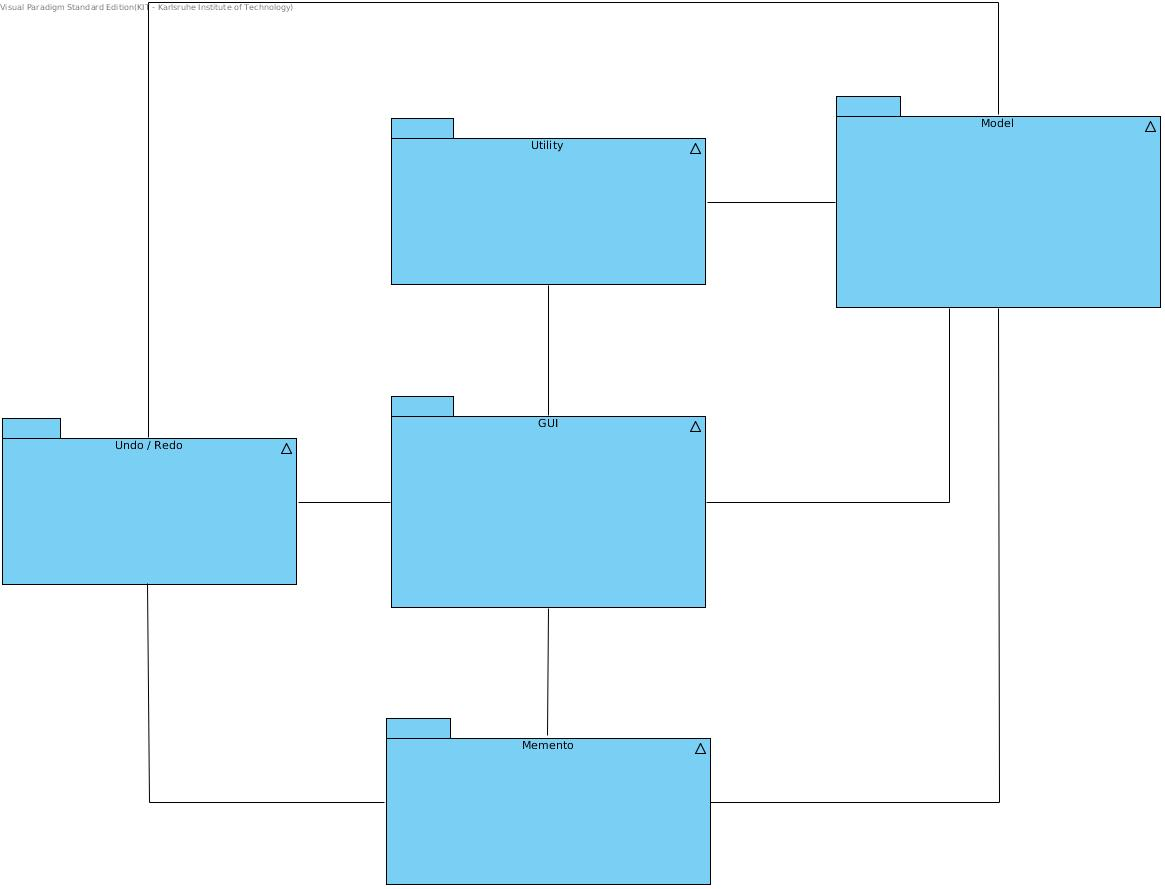
\includegraphics[width=1\textwidth]{Grobuebersicht.jpg}}\\
\newpage
Utility Package\\\\
{\centering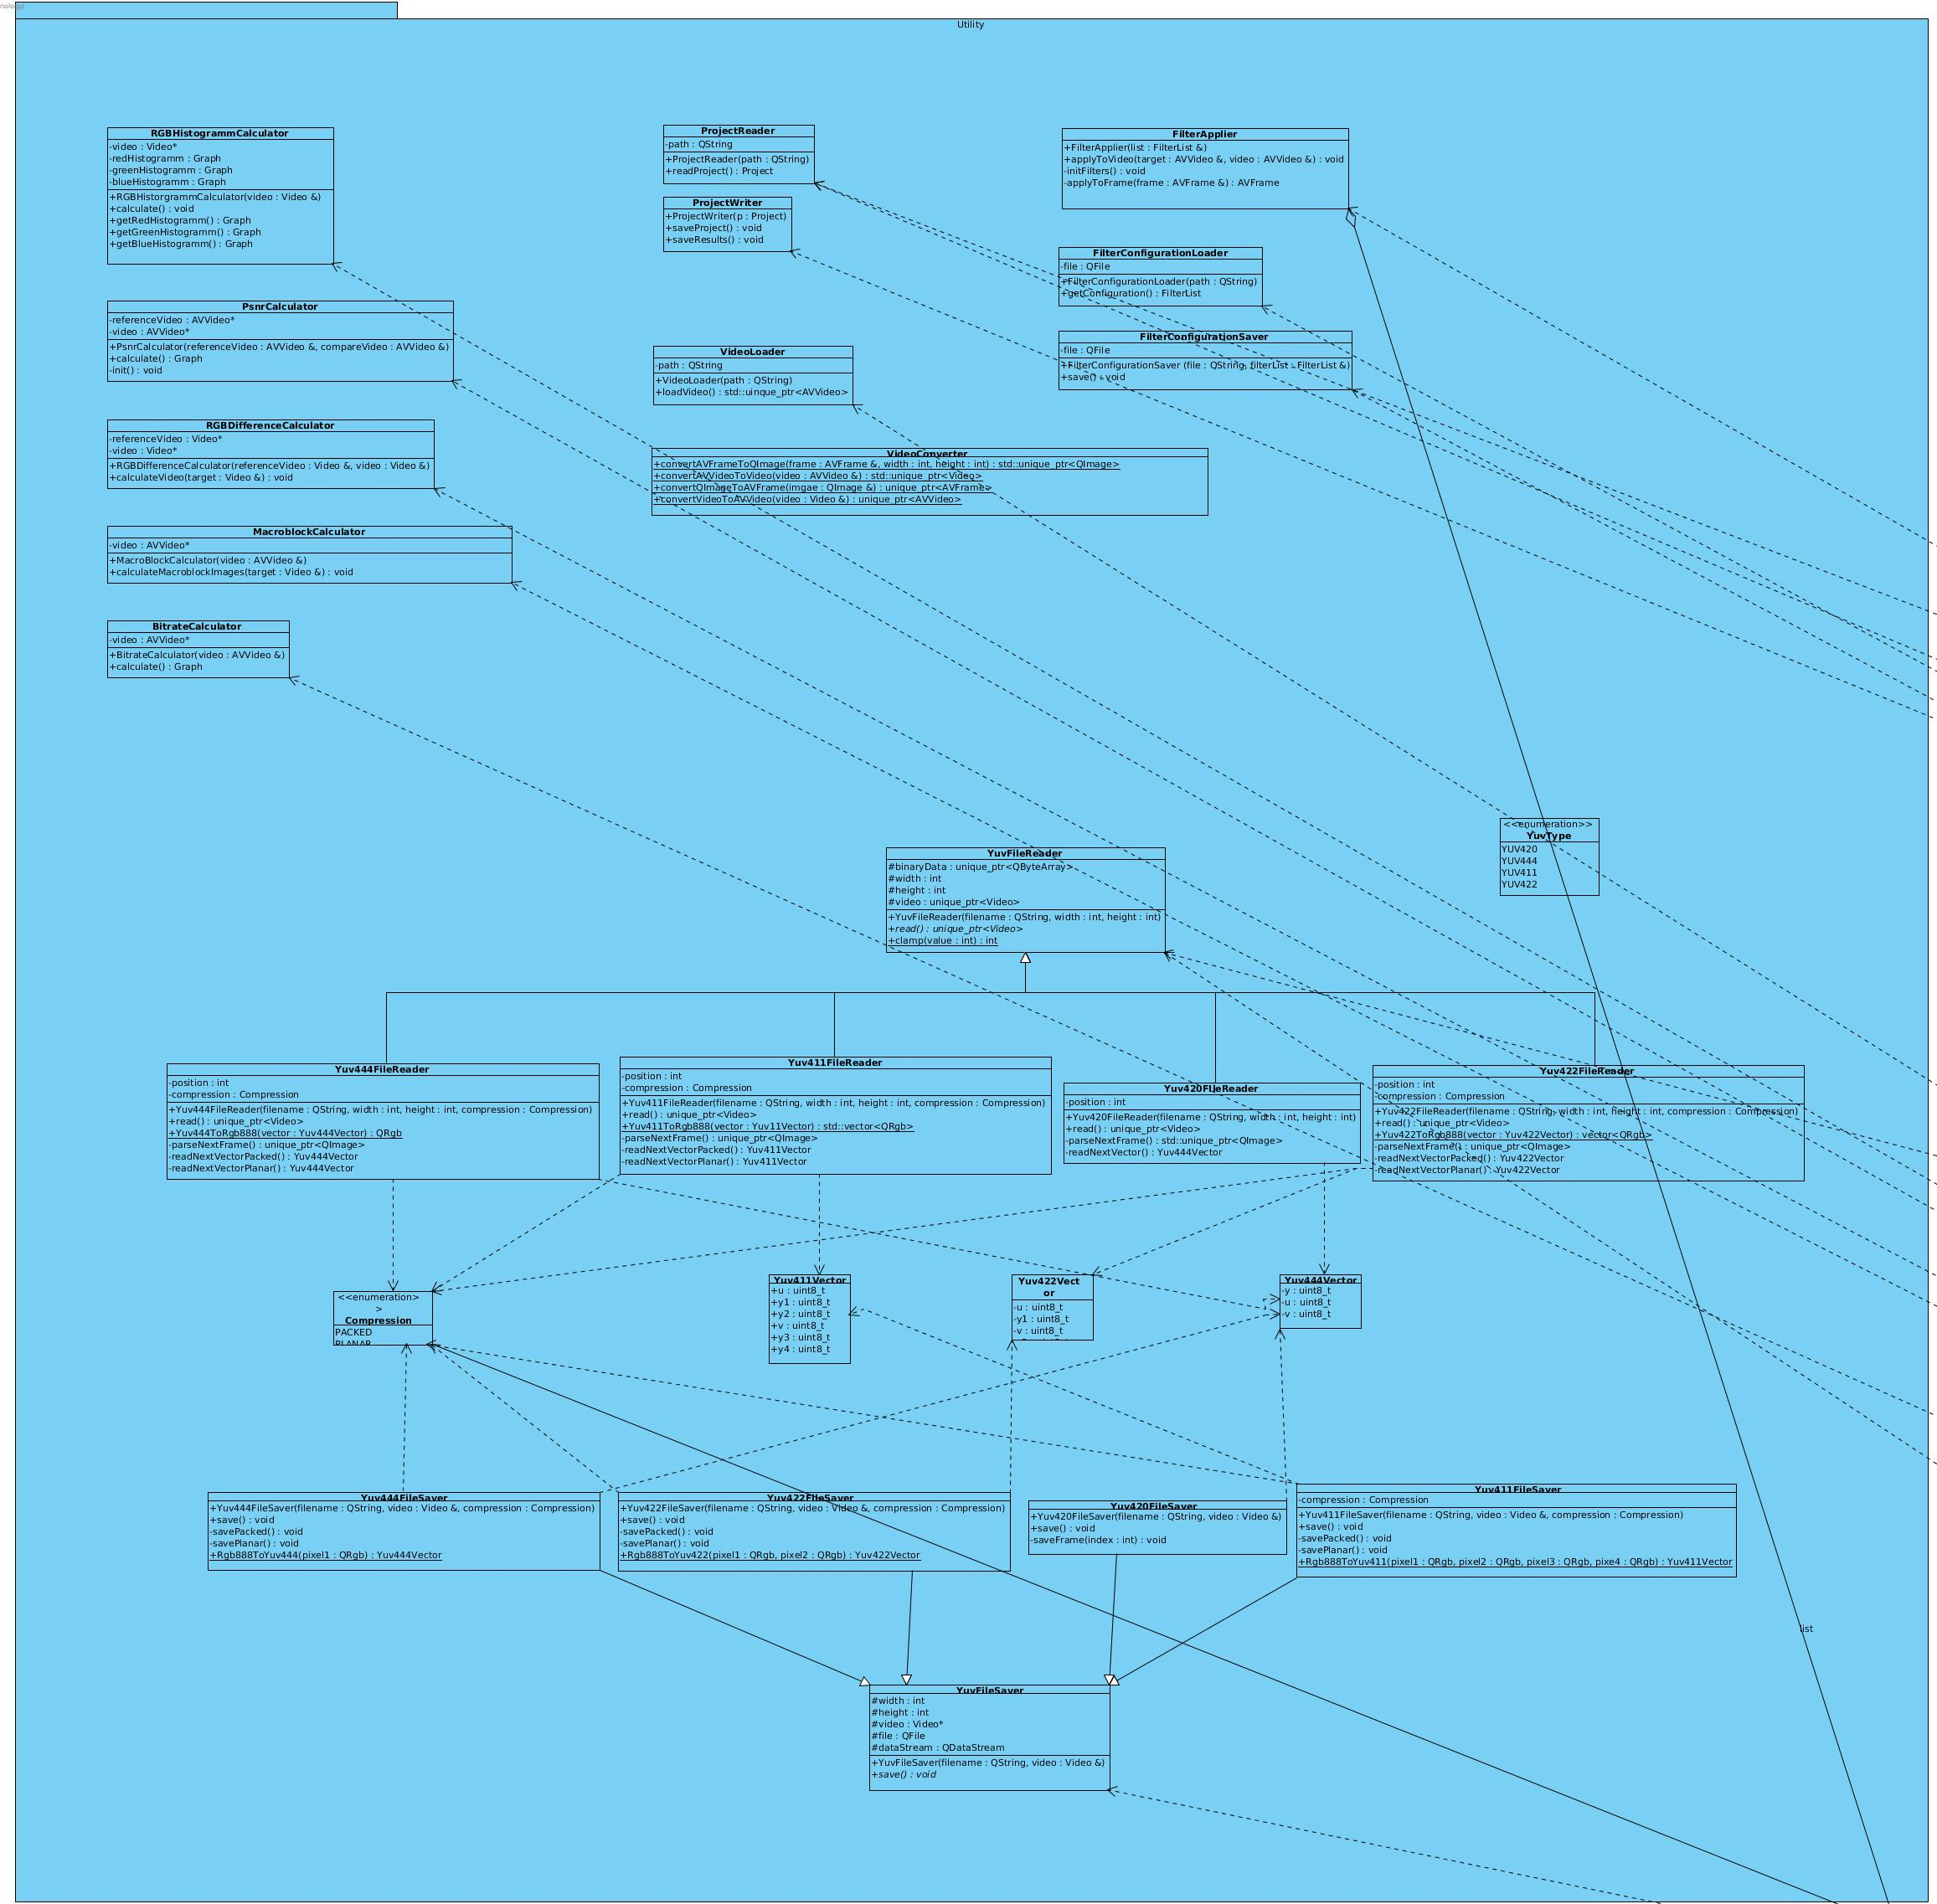
\includegraphics[width=1\textwidth]{Utility.jpg}}\\
\newpage
Model without the filters\\\\
{\centering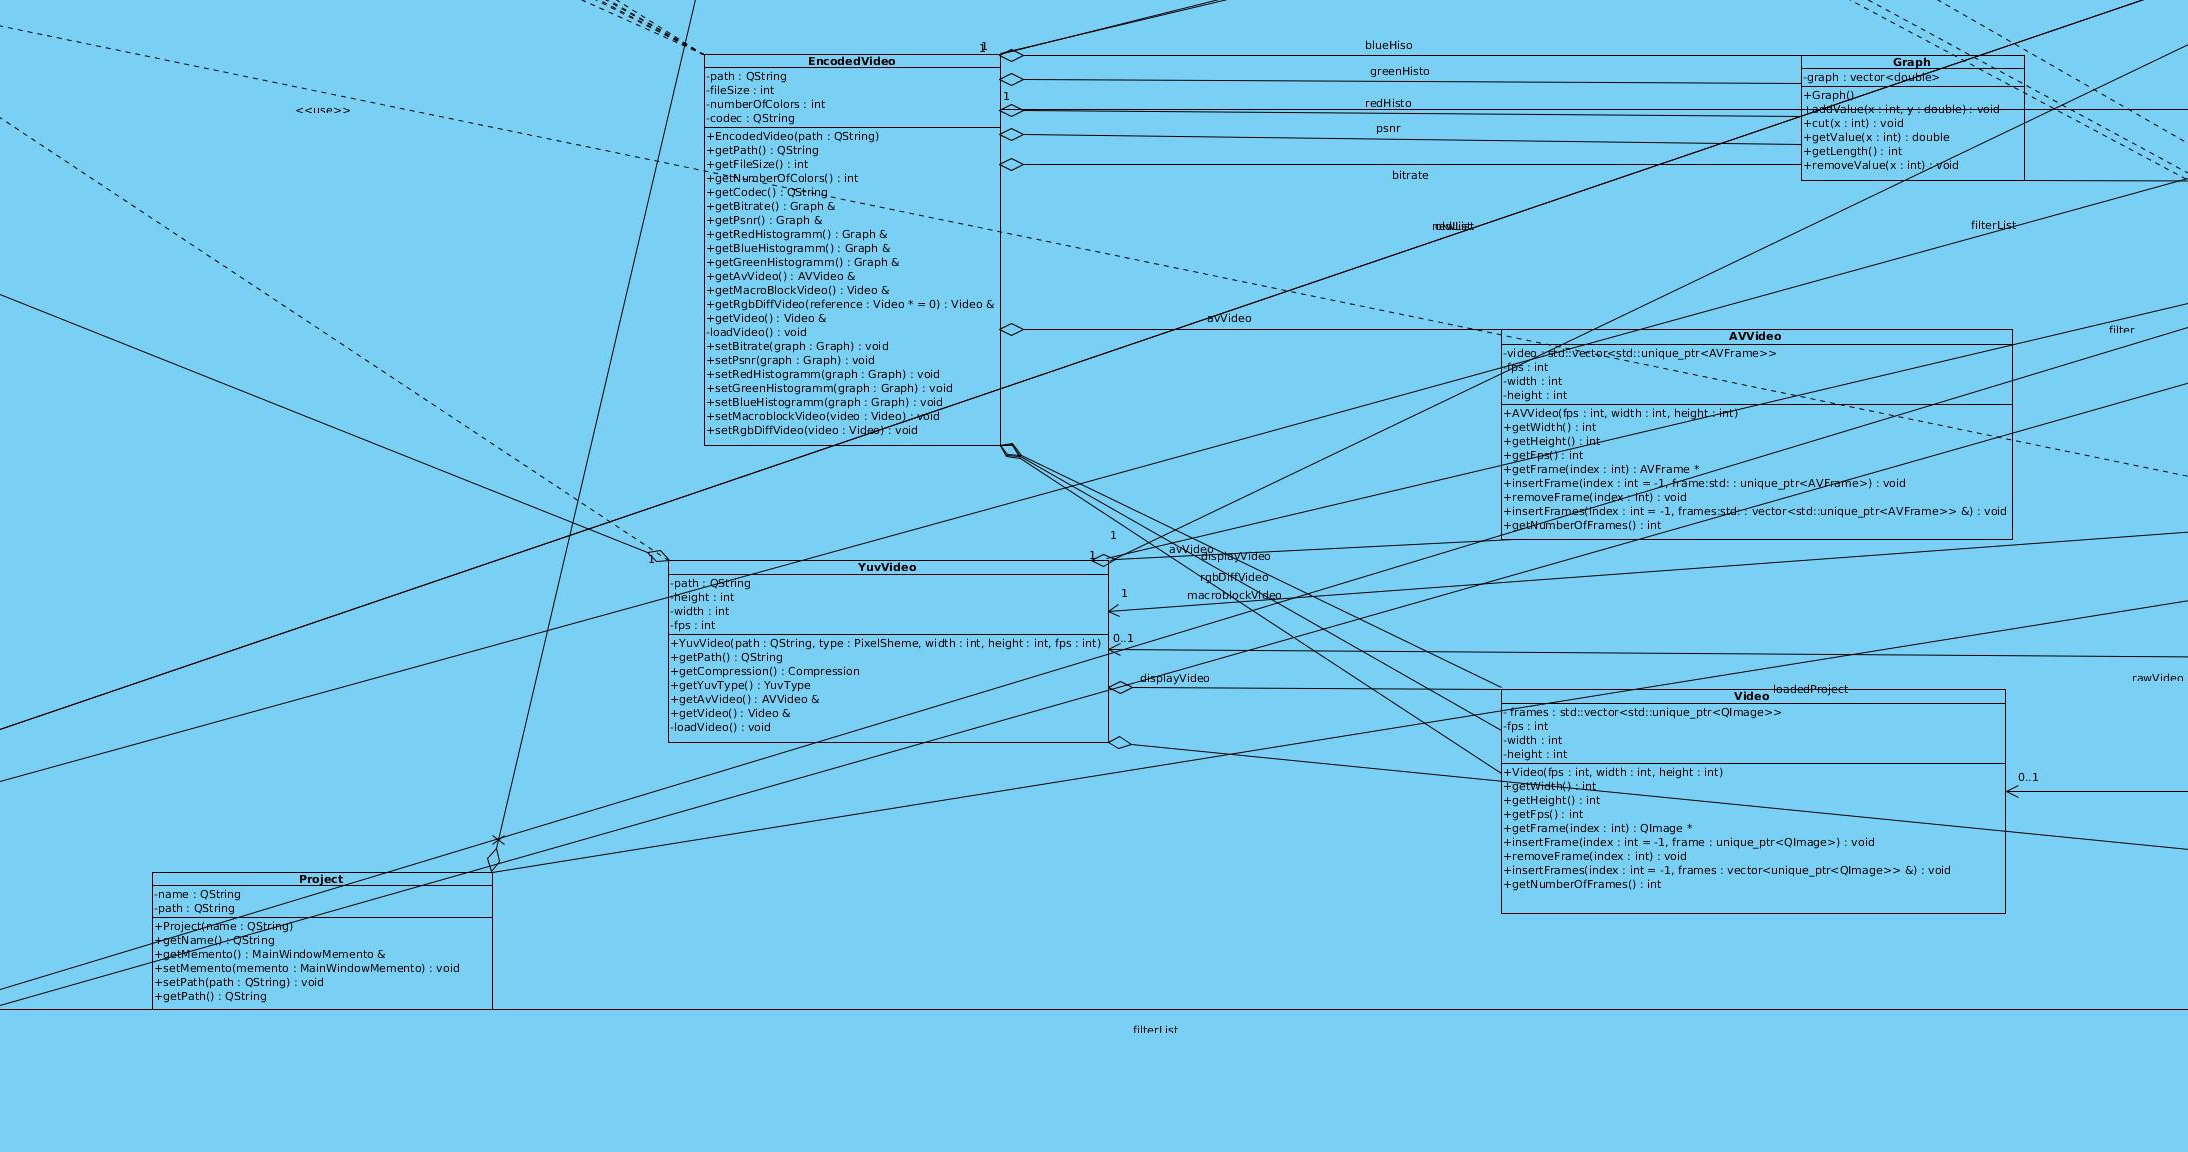
\includegraphics[width=1\textwidth]{Model_noFilter.jpg}}\\
\newpage
GUI without filterboxes\\\\
{\centering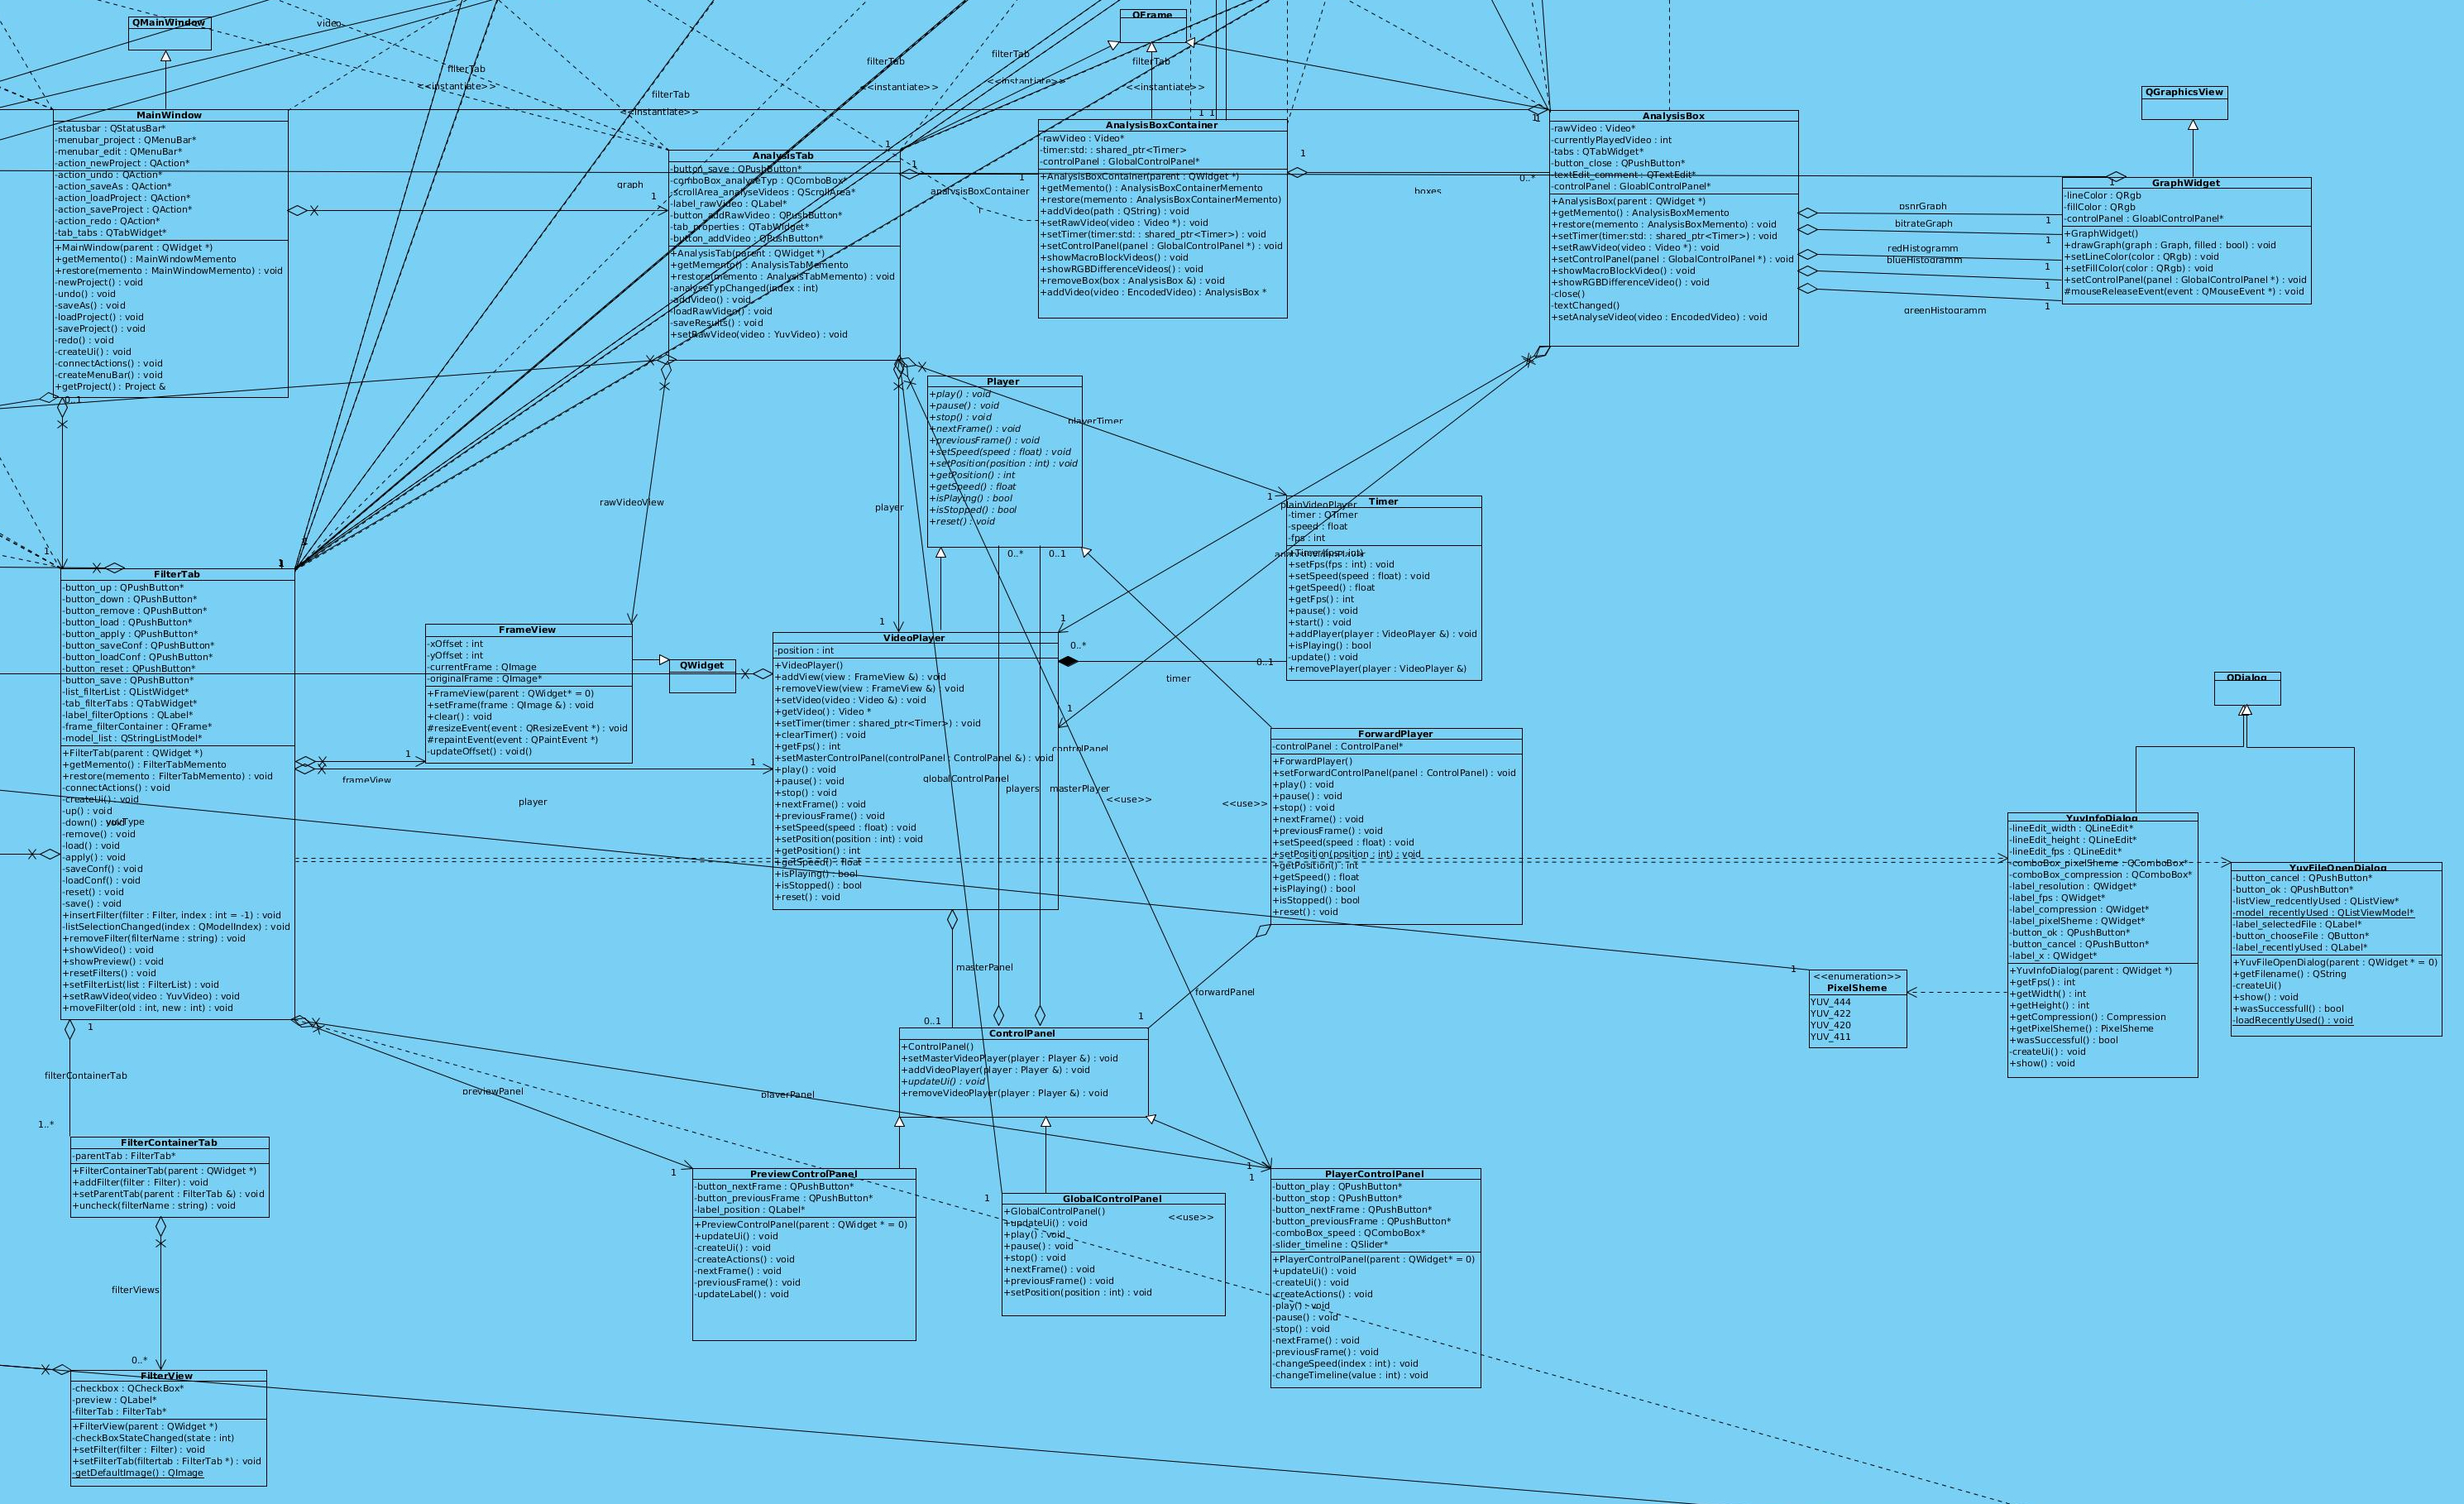
\includegraphics[width=1\textwidth]{GUI_noFilter.jpg}}\\
\newpage
Memento Package\\\\
{\centering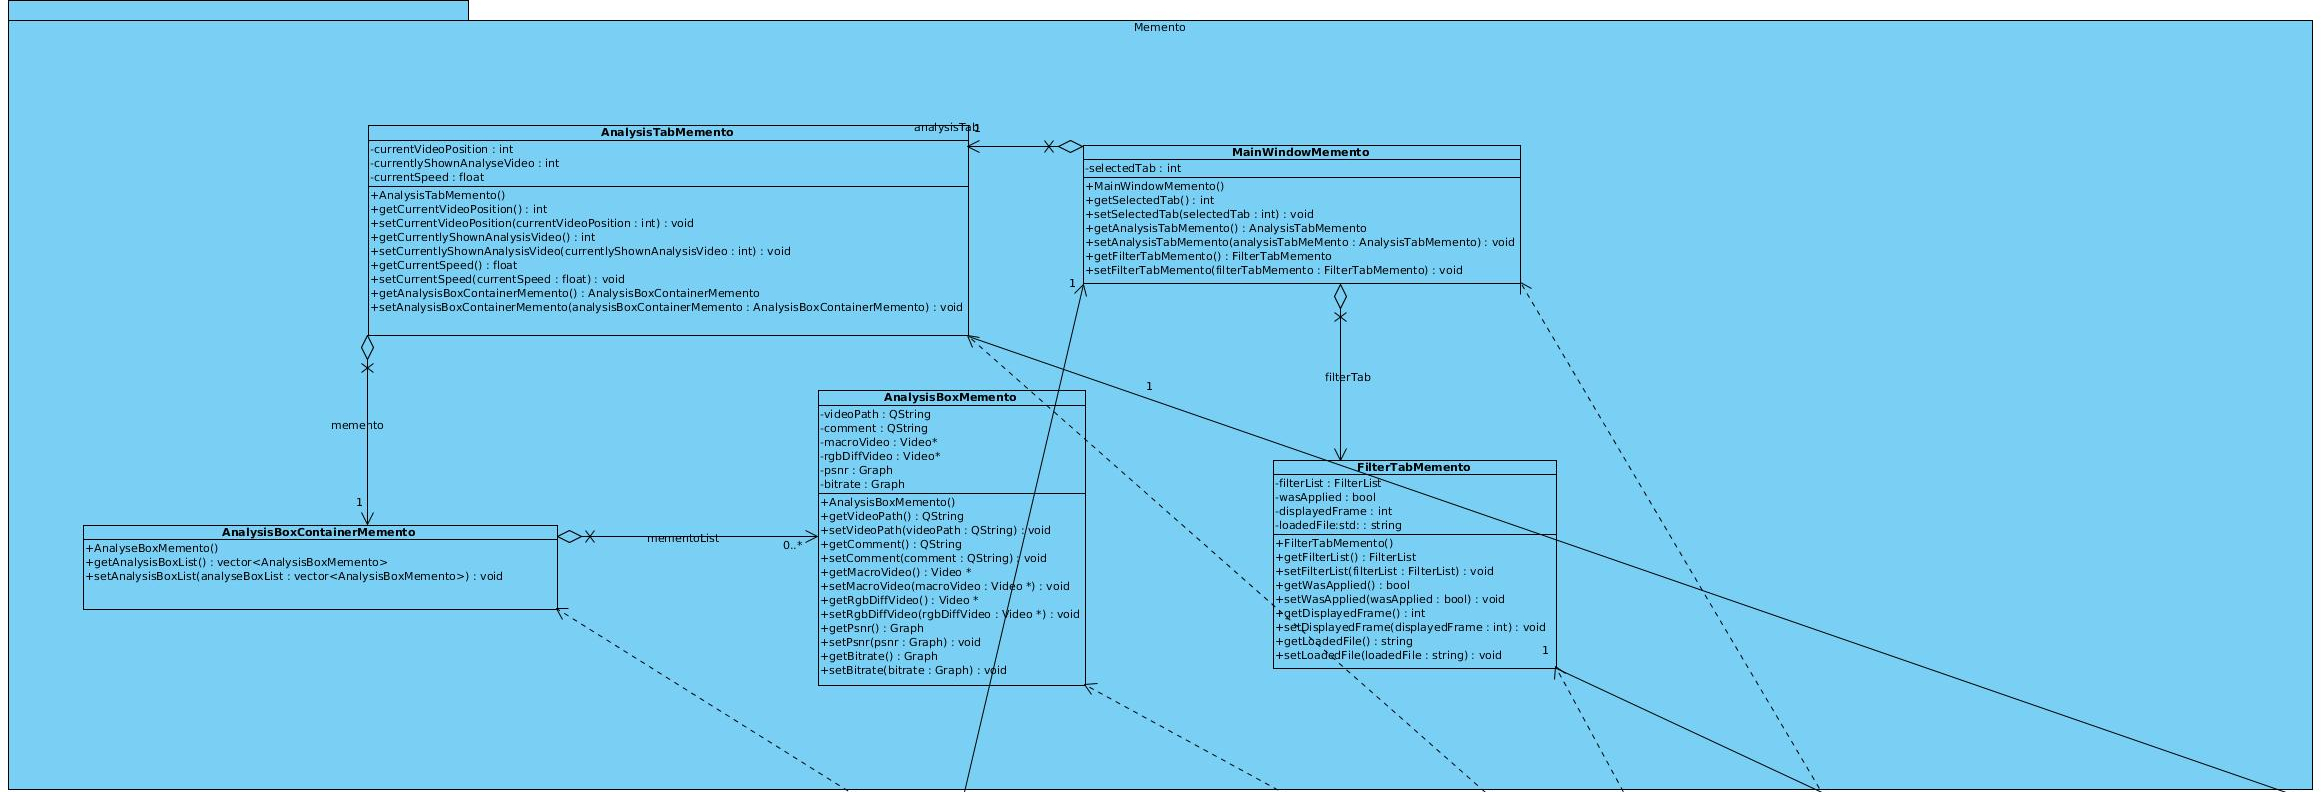
\includegraphics[width=1\textwidth]{Memento.jpg}}\\\\\\
Undo/Redo Package\\\\
{\centering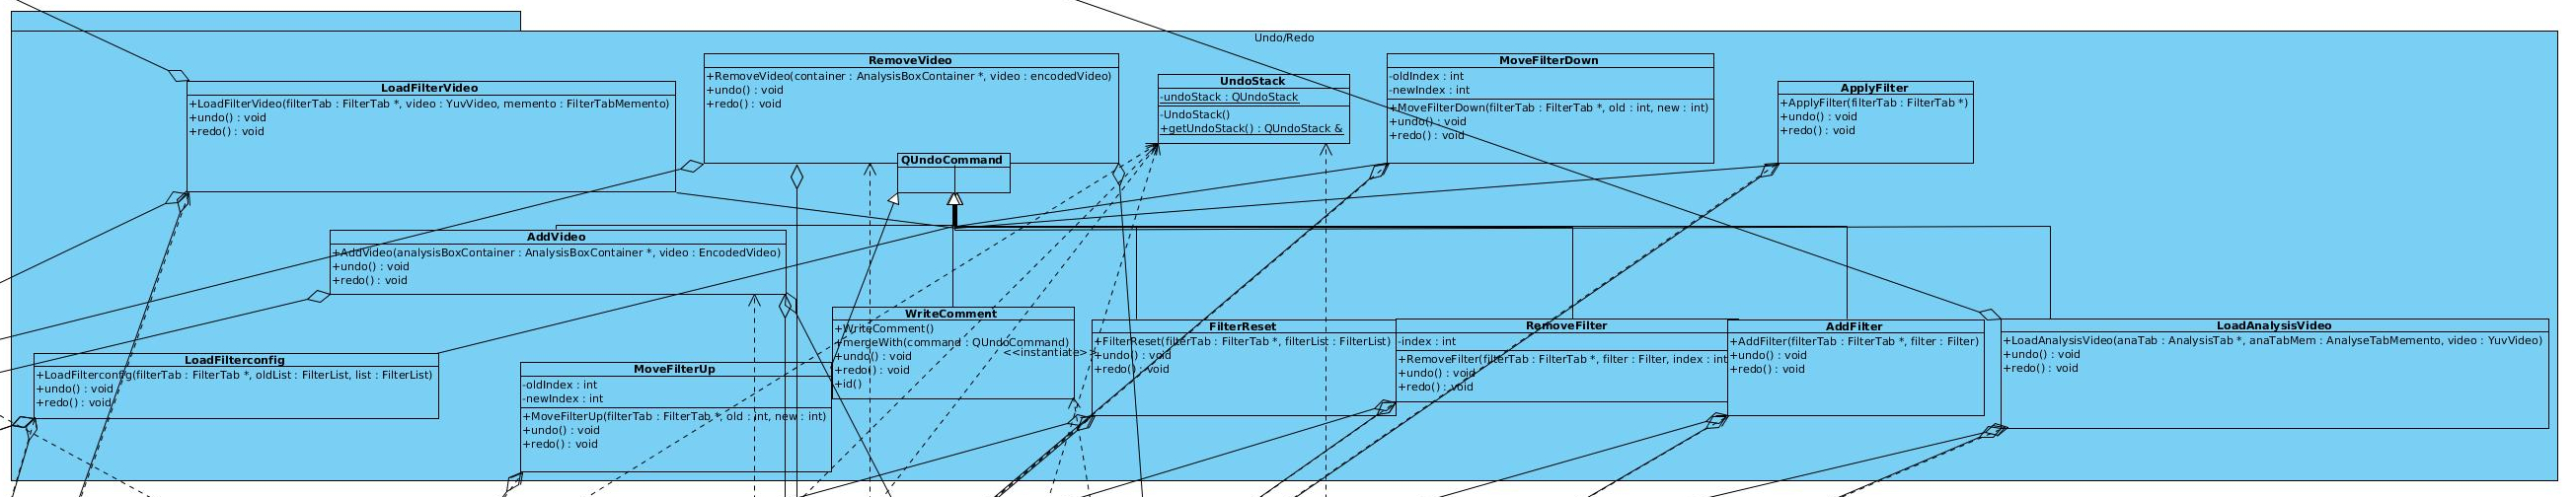
\includegraphics[width=1\textwidth]{UndoRedo.jpg}}\\
\newpage
\section{Sequence Diagrams}
\subsection*{LoadVideo sequence diagram}
{\centering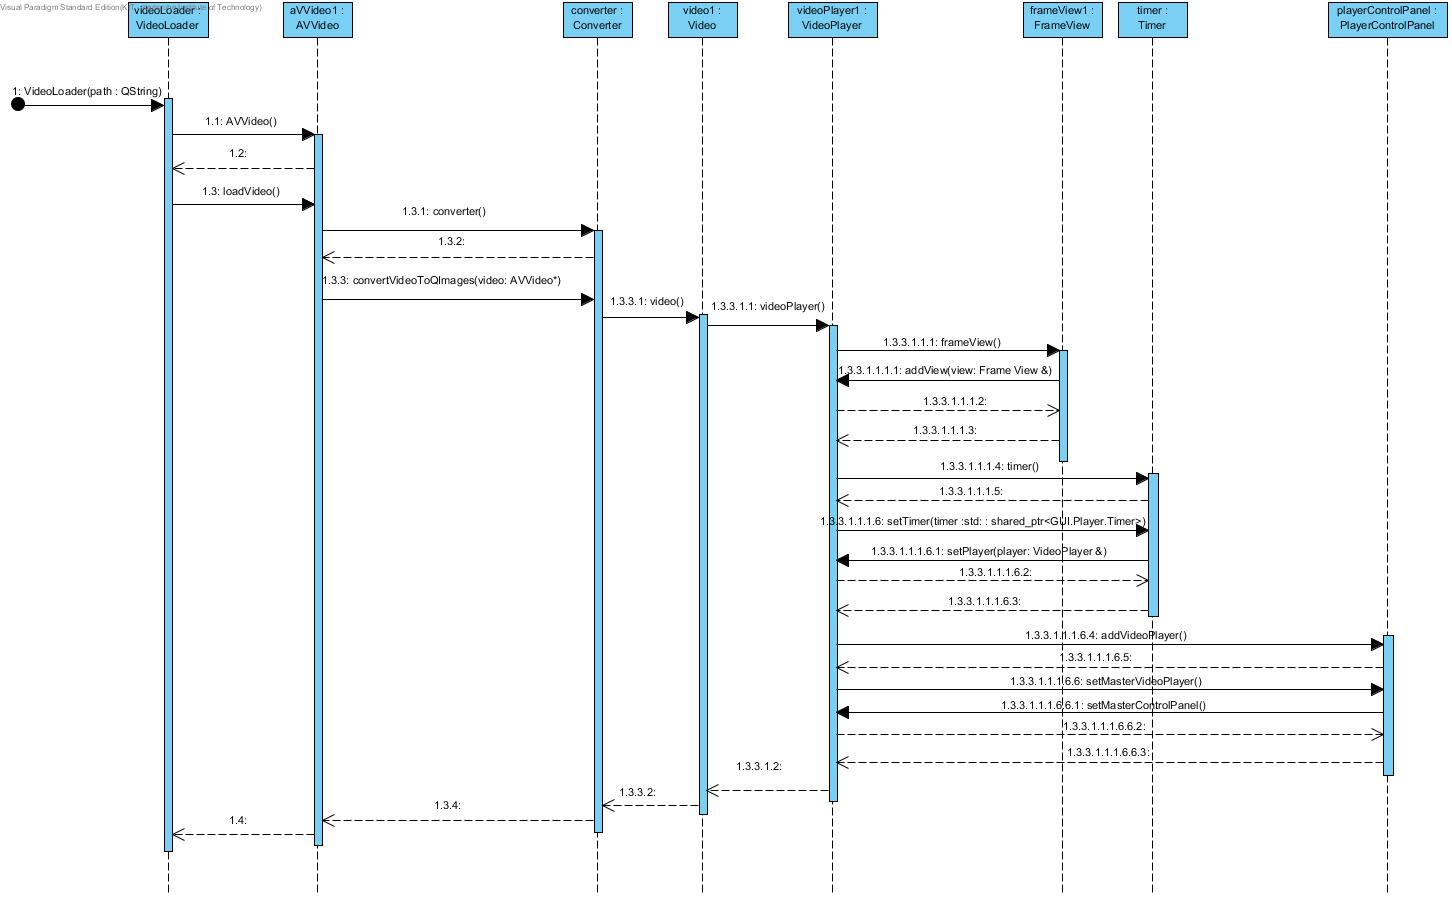
\includegraphics[width=1\textwidth]{SequenceDiagram1.jpg}}\\
When you load a new Video a LoadVideo object is created with the path to the Video as a parameter.Then a AVVideo is created and with the Converter a Video which is then given to a VideoPlayer. This VideoPlayer has a FrameView a Timer and is then given to a ControlPanel
\newpage
\subsection*{Analysis sequence diagram}
{\centering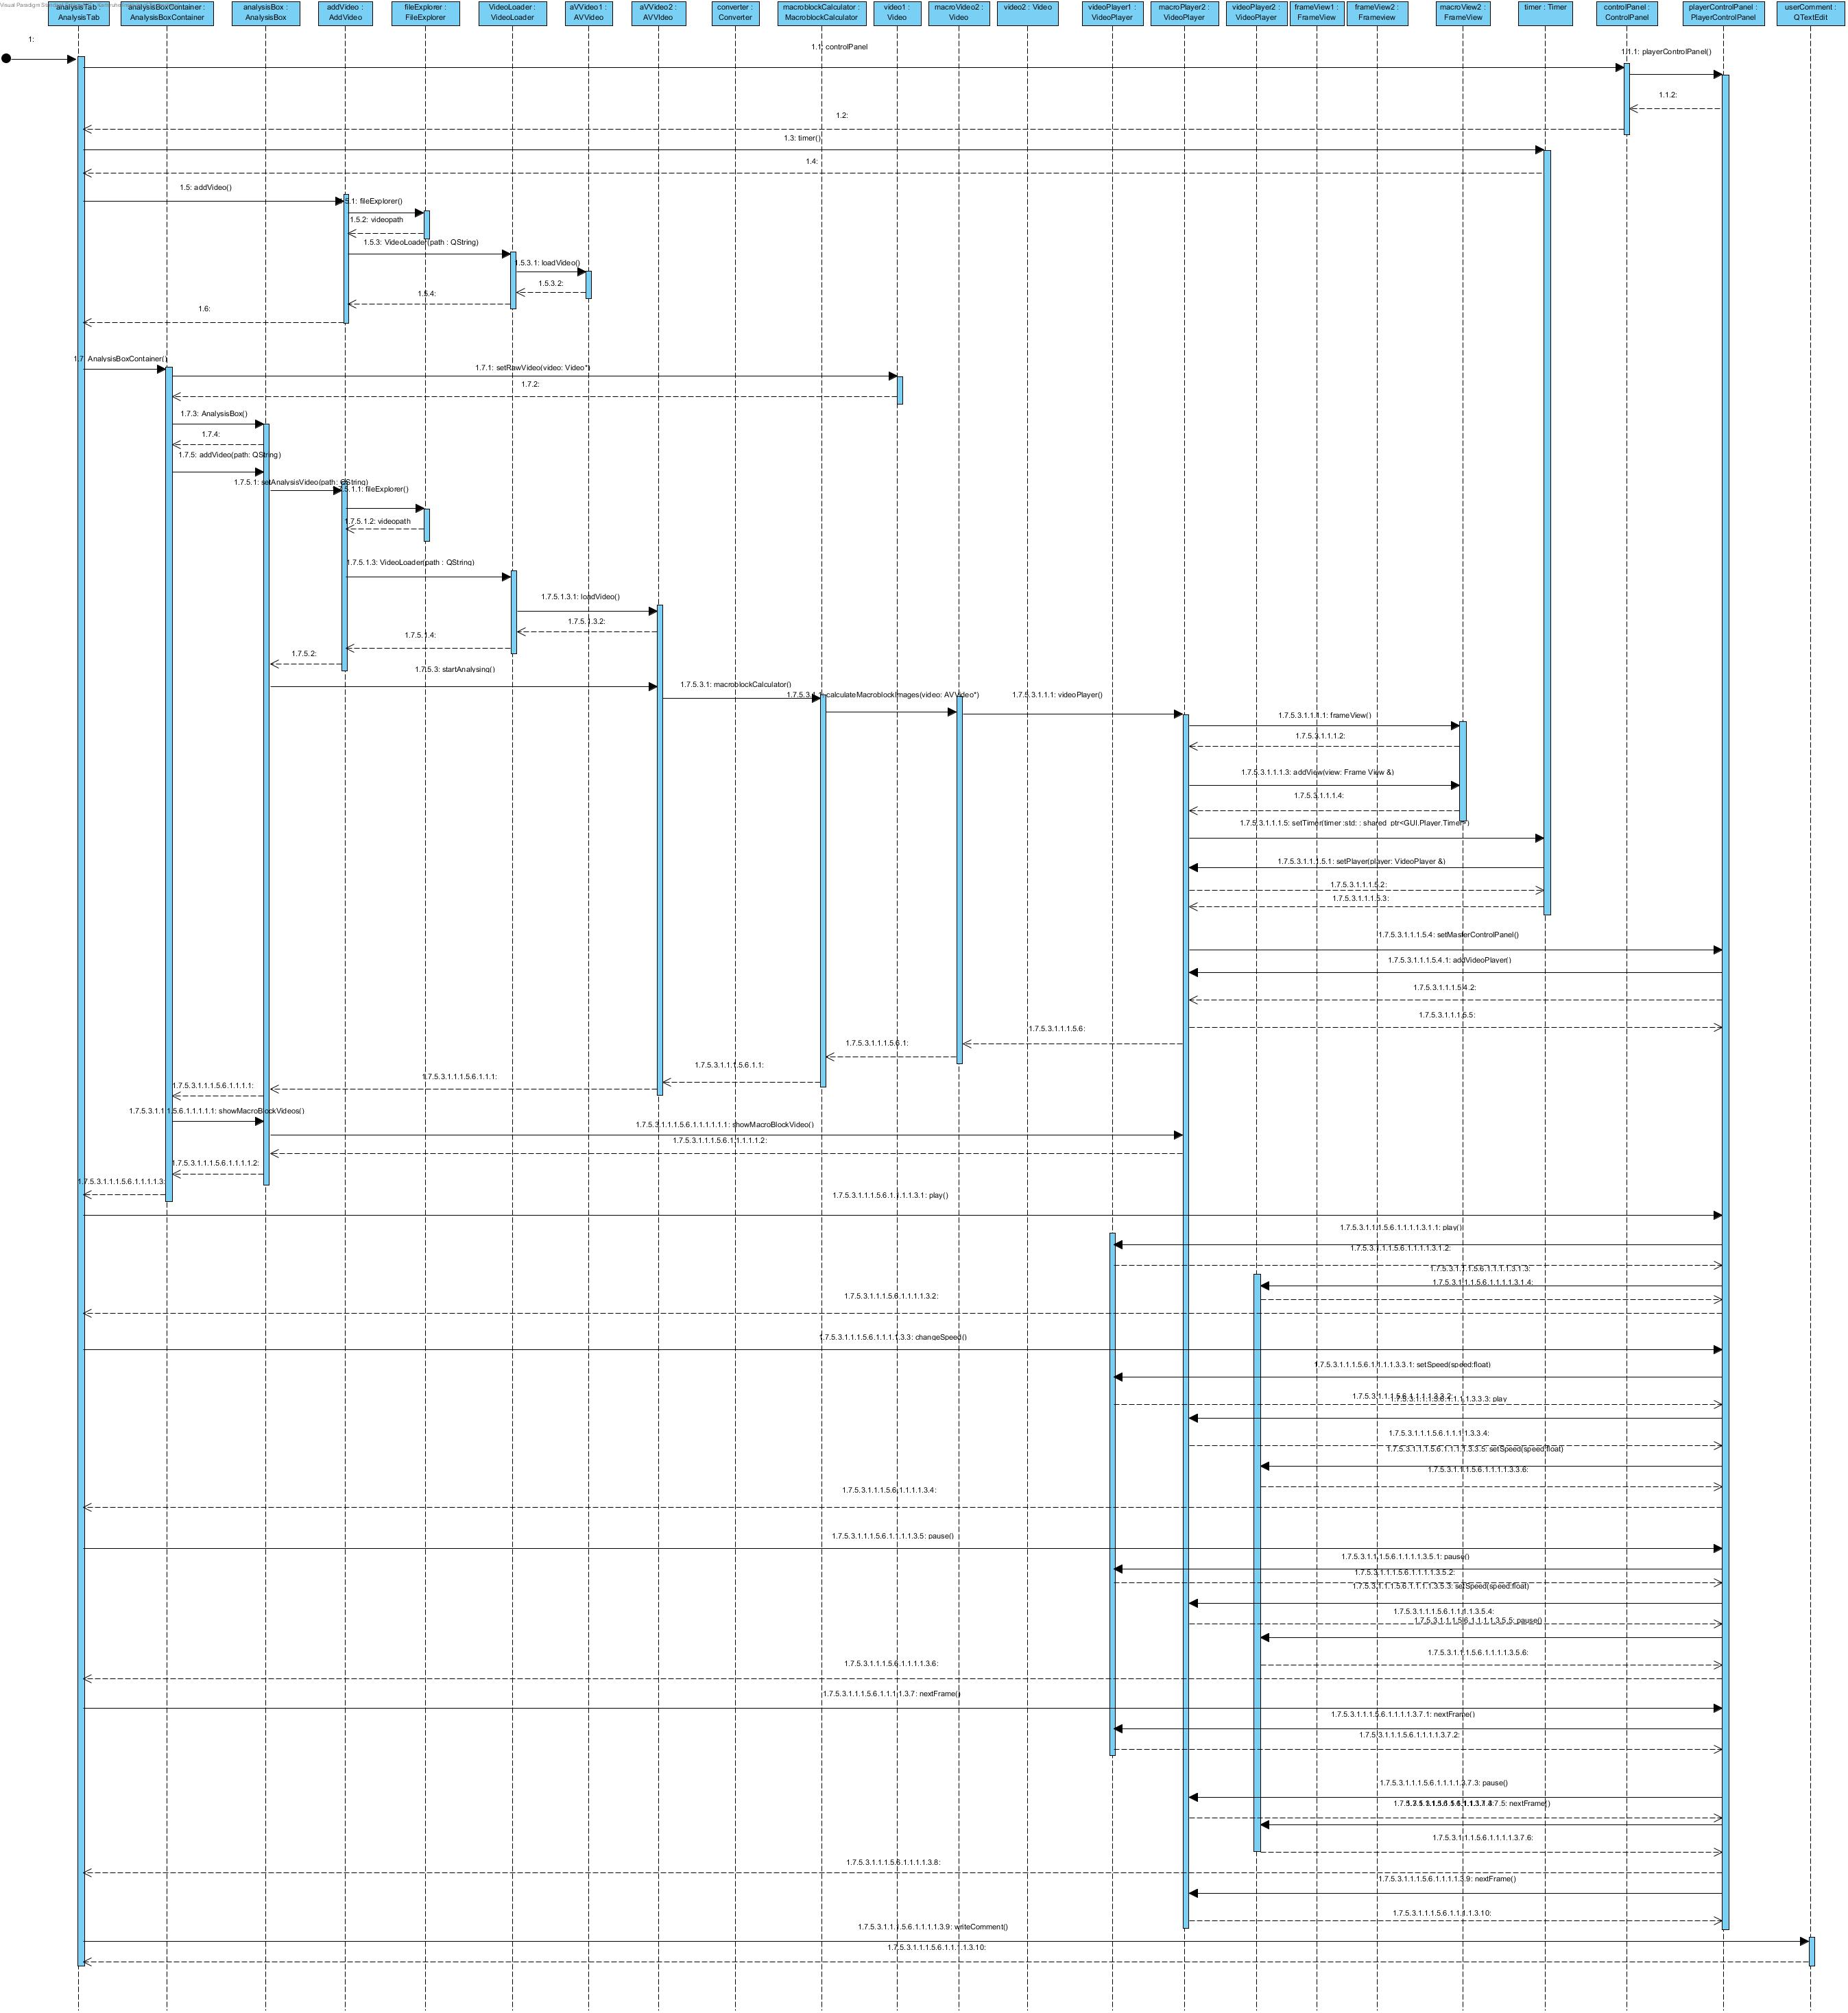
\includegraphics[width=1\textwidth]{SequenceDiagram2.jpg}}\\
First a ControlPanel and a PlayerControlPanel are created. When a Video is added the LoadVideo Sequenz which is descriped above is initiated.  If an additional Video is added  
an AnalysisBox is created in which the added Video is loaded and the Analysis starts in which he MacroblocVideo is calculated and Displayed in a second VideoPlayer.
When play is pressed in the ControlPanel all Videos start to play.
\newpage
\subsection*{Filter sequence diagram}
{\centering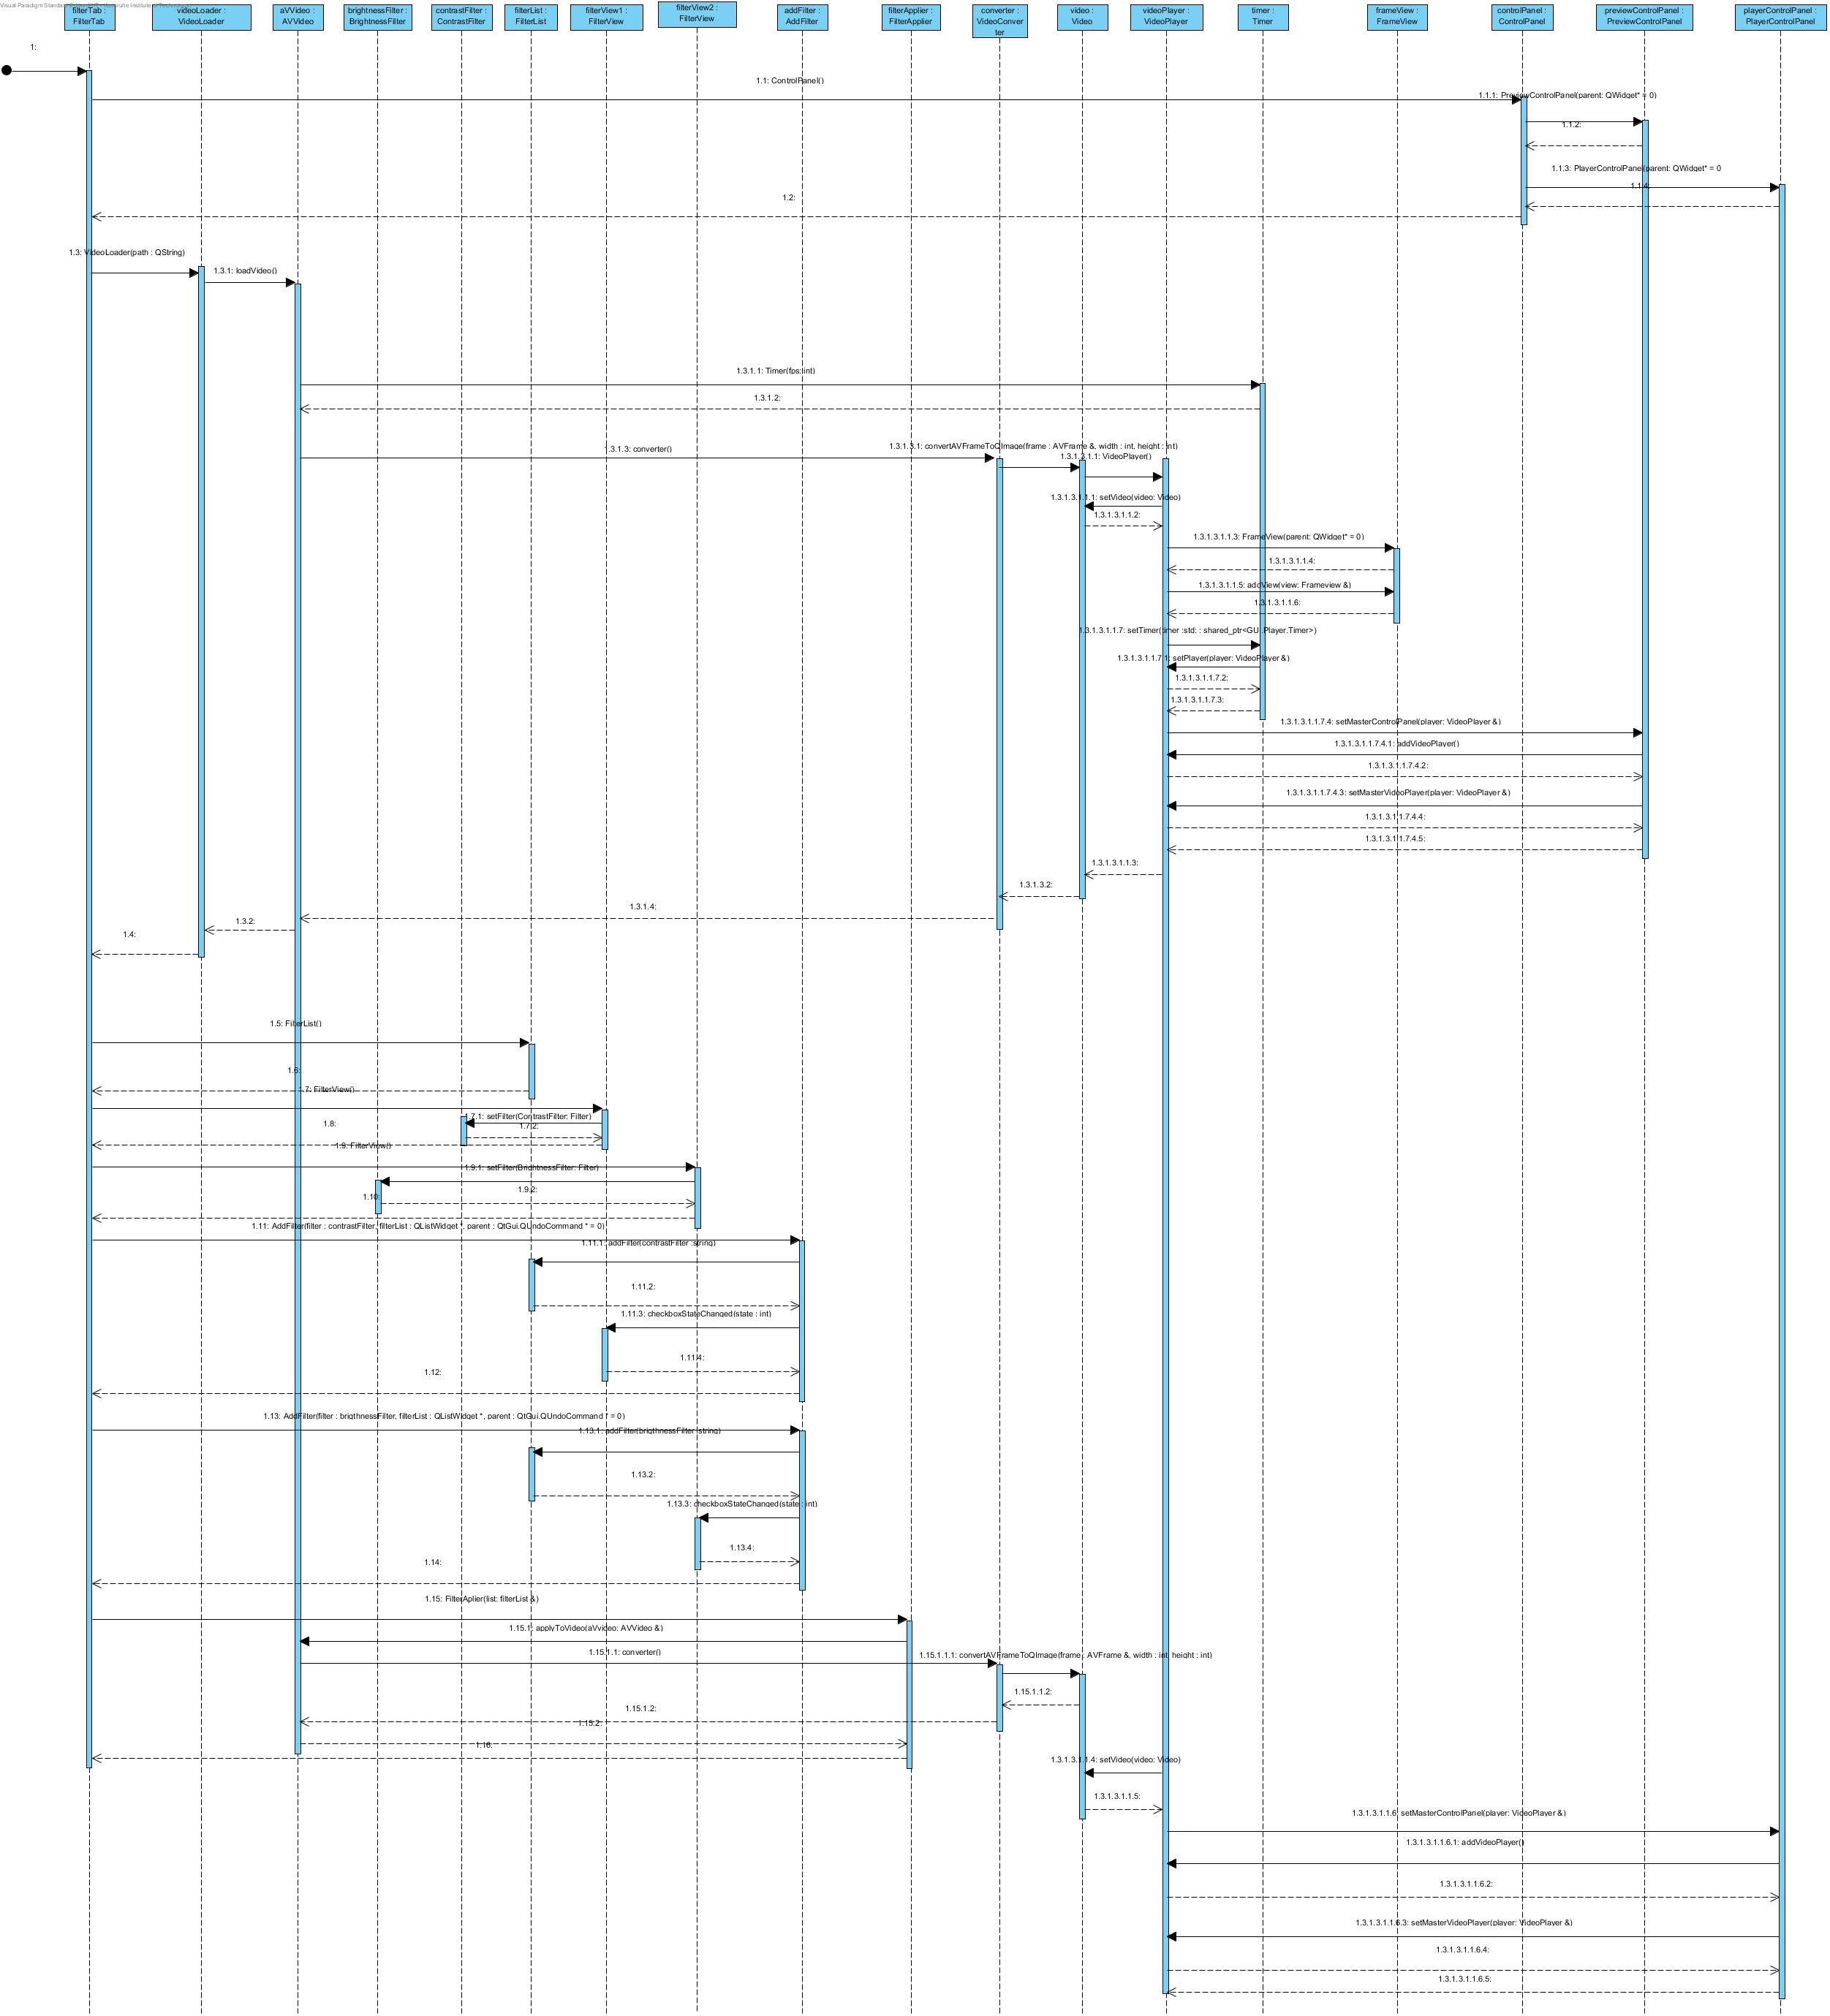
\includegraphics[width=1\textwidth]{SequenceDiagram3.jpg}}\\
First the ControlPanel, PlayerControlPanel and PreviewControlPanel are created.
Then a Video is loaded with the LoadVideo sequenz. Then a Filter are added to the FilterList. This FilterLis is then applied to the AVVideo which is the converted to an Video and Displayed in the VideoPlayer.
\chapter{Namespace Documentation}
\hypertarget{namespaceGUI}{}\section{G\+U\+I Namespace Reference}
\label{namespaceGUI}\index{G\+U\+I@{G\+U\+I}}
\subsection*{Namespaces}
\begin{DoxyCompactItemize}
\item 
 \hyperlink{namespaceGUI_1_1Player}{Player}
\item 
 \hyperlink{namespaceGUI_1_1QtGui}{Qt\+Gui}
\end{DoxyCompactItemize}
\subsection*{Data Structures}
\begin{DoxyCompactItemize}
\item 
class \hyperlink{classGUI_1_1AnalysisBox}{Analysis\+Box}
\item 
class \hyperlink{classGUI_1_1AnalysisBoxContainer}{Analysis\+Box\+Container}
\item 
class \hyperlink{classGUI_1_1AnalysisTab}{Analysis\+Tab}
\item 
class \hyperlink{classGUI_1_1BlendingFilterBox}{Blending\+Filter\+Box}
\item 
class \hyperlink{classGUI_1_1BlurFilterBox}{Blur\+Filter\+Box}
\item 
class \hyperlink{classGUI_1_1BorderFilterBox}{Border\+Filter\+Box}
\item 
class \hyperlink{classGUI_1_1BrightnessFilterBox}{Brightness\+Filter\+Box}
\item 
class \hyperlink{classGUI_1_1ColorbalanceFilterBox}{Colorbalance\+Filter\+Box}
\item 
class \hyperlink{classGUI_1_1ContrastFilterBox}{Contrast\+Filter\+Box}
\item 
class \hyperlink{classGUI_1_1FilterConfigurationBox}{Filter\+Configuration\+Box}
\item 
class \hyperlink{classGUI_1_1FilterContainerTab}{Filter\+Container\+Tab}
\item 
class \hyperlink{classGUI_1_1FilterTab}{Filter\+Tab}
\item 
class \hyperlink{classGUI_1_1FilterView}{Filter\+View}
\item 
class \hyperlink{classGUI_1_1ForwardPlayer}{Forward\+Player}
\item 
class \hyperlink{classGUI_1_1GlobalControlPanel}{Global\+Control\+Panel}
\item 
class \hyperlink{classGUI_1_1GraphWidget}{Graph\+Widget}
\item 
class \hyperlink{classGUI_1_1GridFilterBox}{Grid\+Filter\+Box}
\item 
class \hyperlink{classGUI_1_1MainWindow}{Main\+Window}
\item 
class \hyperlink{classGUI_1_1MirrorFilterBox}{Mirror\+Filter\+Box}
\item 
class \hyperlink{classGUI_1_1NoiseFilterBox}{Noise\+Filter\+Box}
\item 
class \hyperlink{classGUI_1_1PlainFilterBox}{Plain\+Filter\+Box}
\item 
class \hyperlink{classGUI_1_1PosterFilterBox}{Poster\+Filter\+Box}
\item 
class \hyperlink{classGUI_1_1RectangleFilterBox}{Rectangle\+Filter\+Box}
\item 
class \hyperlink{classGUI_1_1RGBFilterBox}{R\+G\+B\+Filter\+Box}
\item 
class \hyperlink{classGUI_1_1RotationFilterBox}{Rotation\+Filter\+Box}
\item 
class \hyperlink{classGUI_1_1SaturationFilterBox}{Saturation\+Filter\+Box}
\item 
class \hyperlink{classGUI_1_1ScaleFilterBox}{Scale\+Filter\+Box}
\item 
class \hyperlink{classGUI_1_1SharpnessFilterBox}{Sharpness\+Filter\+Box}
\item 
class \hyperlink{classGUI_1_1ZoomFilterBox}{Zoom\+Filter\+Box}
\end{DoxyCompactItemize}

\hypertarget{namespaceMemento}{}\section{Memento Namespace Reference}
\label{namespaceMemento}\index{Memento@{Memento}}
\subsection*{Data Structures}
\begin{DoxyCompactItemize}
\item 
class \hyperlink{classMemento_1_1AnalysisBoxContainerMemento}{Analysis\+Box\+Container\+Memento}
\item 
class \hyperlink{classMemento_1_1AnalysisBoxMemento}{Analysis\+Box\+Memento}
\item 
class \hyperlink{classMemento_1_1AnalysisTabMemento}{Analysis\+Tab\+Memento}
\item 
class \hyperlink{classMemento_1_1FilterTabMemento}{Filter\+Tab\+Memento}
\item 
class \hyperlink{classMemento_1_1MainWindowMemento}{Main\+Window\+Memento}
\end{DoxyCompactItemize}

\hypertarget{namespaceModel}{}\section{Model Namespace Reference}
\label{namespaceModel}\index{Model@{Model}}
\subsection*{Data Structures}
\begin{DoxyCompactItemize}
\item 
class \hyperlink{classModel_1_1AVVideo}{A\+V\+Video}
\item 
class \hyperlink{classModel_1_1BlackWhiteFilter}{Black\+White\+Filter}
\item 
class \hyperlink{classModel_1_1BlendingFilter}{Blending\+Filter}
\item 
class \hyperlink{classModel_1_1BlurFilter}{Blur\+Filter}
\item 
class \hyperlink{classModel_1_1BorderFilter}{Border\+Filter}
\item 
class \hyperlink{classModel_1_1BrightnessFilter}{Brightness\+Filter}
\item 
class \hyperlink{classModel_1_1ColorbalanceFilter}{Colorbalance\+Filter}
\item 
class \hyperlink{classModel_1_1ContrastFilter}{Contrast\+Filter}
\item 
class \hyperlink{classModel_1_1EdgeFilter}{Edge\+Filter}
\item 
class \hyperlink{classModel_1_1EncodedVideo}{Encoded\+Video}
\item 
class \hyperlink{classModel_1_1Filter}{Filter}
\item 
class \hyperlink{classModel_1_1FilterApplier}{Filter\+Applier}
\item 
class \hyperlink{classModel_1_1FilterList}{Filter\+List}
\item 
class \hyperlink{classModel_1_1Graph}{Graph}
\item 
class \hyperlink{classModel_1_1GridFilter}{Grid\+Filter}
\item 
class \hyperlink{classModel_1_1MirrorFilter}{Mirror\+Filter}
\item 
class \hyperlink{classModel_1_1NegativeFilter}{Negative\+Filter}
\item 
class \hyperlink{classModel_1_1NoiseFilter}{Noise\+Filter}
\item 
class \hyperlink{classModel_1_1PosterFilter}{Poster\+Filter}
\item 
class \hyperlink{classModel_1_1Project}{Project}
\item 
class \hyperlink{classModel_1_1RectangleFilter}{Rectangle\+Filter}
\item 
class \hyperlink{classModel_1_1RGBFilter}{R\+G\+B\+Filter}
\item 
class \hyperlink{classModel_1_1RotationFilter}{Rotation\+Filter}
\item 
class \hyperlink{classModel_1_1SaturationFilter}{Saturation\+Filter}
\item 
class \hyperlink{classModel_1_1ScaleFilter}{Scale\+Filter}
\item 
class \hyperlink{classModel_1_1SepiaFilter}{Sepia\+Filter}
\item 
class \hyperlink{classModel_1_1SharpnessFilter}{Sharpness\+Filter}
\item 
class \hyperlink{classModel_1_1VintageFilter}{Vintage\+Filter}
\item 
class \hyperlink{classModel_1_1YuvVideo}{Yuv\+Video}
\item 
class \hyperlink{classModel_1_1ZoomFilter}{Zoom\+Filter}
\end{DoxyCompactItemize}
\subsection*{Enumerations}
\begin{DoxyCompactItemize}
\item 
enum \hyperlink{namespaceModel_a54742b2fc8f6a246926cbb87b7fae1a4}{Basic\+Color} \{ \hyperlink{namespaceModel_a54742b2fc8f6a246926cbb87b7fae1a4af80f9a890089d211842d59625e561f88}{R\+E\+D}, 
\hyperlink{namespaceModel_a54742b2fc8f6a246926cbb87b7fae1a4aa60bd322f93178d68184e30e162571ca}{G\+R\+E\+E\+N}, 
\hyperlink{namespaceModel_a54742b2fc8f6a246926cbb87b7fae1a4a35d6719cb4d7577c031b3d79057a1b79}{B\+L\+U\+E}
 \}
\item 
enum \hyperlink{namespaceModel_a8a20195c97d8c704572b5922370c2fbc}{Mirror\+Mode} \{ \hyperlink{namespaceModel_a8a20195c97d8c704572b5922370c2fbca4dd51ad73508d6fc83a502966779e48e}{H\+O\+R\+I\+Z\+O\+N\+T\+A\+L}, 
\hyperlink{namespaceModel_a8a20195c97d8c704572b5922370c2fbca1a88641fcd39f2ed3e58a18526e97138}{V\+E\+R\+T\+I\+C\+A\+L}
 \}
\item 
enum \hyperlink{namespaceModel_a0466e3095e9c21e5864d8964e9d7df59}{Noise\+Mode} \{ \hyperlink{namespaceModel_a0466e3095e9c21e5864d8964e9d7df59ae55a36a850c67d46b3b3325de7fce0b8}{S\+T\+A\+T\+I\+C}, 
\hyperlink{namespaceModel_a0466e3095e9c21e5864d8964e9d7df59aa2b65445a3a16f164c5e811064d75726}{R\+A\+N\+D\+O\+M}, 
\hyperlink{namespaceModel_a0466e3095e9c21e5864d8964e9d7df59abdc738e06735e7d289096acf524331c0}{M\+U\+S\+T\+E\+R}
 \}
\end{DoxyCompactItemize}


\subsection{Enumeration Type Documentation}
\hypertarget{namespaceModel_a54742b2fc8f6a246926cbb87b7fae1a4}{}\index{Model@{Model}!Basic\+Color@{Basic\+Color}}
\index{Basic\+Color@{Basic\+Color}!Model@{Model}}
\subsubsection[{Basic\+Color}]{\setlength{\rightskip}{0pt plus 5cm}enum {\bf Basic\+Color}}\label{namespaceModel_a54742b2fc8f6a246926cbb87b7fae1a4}
\begin{Desc}
\item[Enumerator]\par
\begin{description}
\index{R\+E\+D@{R\+E\+D}!Model@{Model}}\index{Model@{Model}!R\+E\+D@{R\+E\+D}}\item[{\em 
\hypertarget{namespaceModel_a54742b2fc8f6a246926cbb87b7fae1a4af80f9a890089d211842d59625e561f88}{}R\+E\+D\label{namespaceModel_a54742b2fc8f6a246926cbb87b7fae1a4af80f9a890089d211842d59625e561f88}
}]\index{G\+R\+E\+E\+N@{G\+R\+E\+E\+N}!Model@{Model}}\index{Model@{Model}!G\+R\+E\+E\+N@{G\+R\+E\+E\+N}}\item[{\em 
\hypertarget{namespaceModel_a54742b2fc8f6a246926cbb87b7fae1a4aa60bd322f93178d68184e30e162571ca}{}G\+R\+E\+E\+N\label{namespaceModel_a54742b2fc8f6a246926cbb87b7fae1a4aa60bd322f93178d68184e30e162571ca}
}]\index{B\+L\+U\+E@{B\+L\+U\+E}!Model@{Model}}\index{Model@{Model}!B\+L\+U\+E@{B\+L\+U\+E}}\item[{\em 
\hypertarget{namespaceModel_a54742b2fc8f6a246926cbb87b7fae1a4a35d6719cb4d7577c031b3d79057a1b79}{}B\+L\+U\+E\label{namespaceModel_a54742b2fc8f6a246926cbb87b7fae1a4a35d6719cb4d7577c031b3d79057a1b79}
}]\end{description}
\end{Desc}
\hypertarget{namespaceModel_a8a20195c97d8c704572b5922370c2fbc}{}\index{Model@{Model}!Mirror\+Mode@{Mirror\+Mode}}
\index{Mirror\+Mode@{Mirror\+Mode}!Model@{Model}}
\subsubsection[{Mirror\+Mode}]{\setlength{\rightskip}{0pt plus 5cm}enum {\bf Mirror\+Mode}}\label{namespaceModel_a8a20195c97d8c704572b5922370c2fbc}
\begin{Desc}
\item[Enumerator]\par
\begin{description}
\index{H\+O\+R\+I\+Z\+O\+N\+T\+A\+L@{H\+O\+R\+I\+Z\+O\+N\+T\+A\+L}!Model@{Model}}\index{Model@{Model}!H\+O\+R\+I\+Z\+O\+N\+T\+A\+L@{H\+O\+R\+I\+Z\+O\+N\+T\+A\+L}}\item[{\em 
\hypertarget{namespaceModel_a8a20195c97d8c704572b5922370c2fbca4dd51ad73508d6fc83a502966779e48e}{}H\+O\+R\+I\+Z\+O\+N\+T\+A\+L\label{namespaceModel_a8a20195c97d8c704572b5922370c2fbca4dd51ad73508d6fc83a502966779e48e}
}]\index{V\+E\+R\+T\+I\+C\+A\+L@{V\+E\+R\+T\+I\+C\+A\+L}!Model@{Model}}\index{Model@{Model}!V\+E\+R\+T\+I\+C\+A\+L@{V\+E\+R\+T\+I\+C\+A\+L}}\item[{\em 
\hypertarget{namespaceModel_a8a20195c97d8c704572b5922370c2fbca1a88641fcd39f2ed3e58a18526e97138}{}V\+E\+R\+T\+I\+C\+A\+L\label{namespaceModel_a8a20195c97d8c704572b5922370c2fbca1a88641fcd39f2ed3e58a18526e97138}
}]\end{description}
\end{Desc}
\hypertarget{namespaceModel_a0466e3095e9c21e5864d8964e9d7df59}{}\index{Model@{Model}!Noise\+Mode@{Noise\+Mode}}
\index{Noise\+Mode@{Noise\+Mode}!Model@{Model}}
\subsubsection[{Noise\+Mode}]{\setlength{\rightskip}{0pt plus 5cm}enum {\bf Noise\+Mode}}\label{namespaceModel_a0466e3095e9c21e5864d8964e9d7df59}
\begin{Desc}
\item[Enumerator]\par
\begin{description}
\index{S\+T\+A\+T\+I\+C@{S\+T\+A\+T\+I\+C}!Model@{Model}}\index{Model@{Model}!S\+T\+A\+T\+I\+C@{S\+T\+A\+T\+I\+C}}\item[{\em 
\hypertarget{namespaceModel_a0466e3095e9c21e5864d8964e9d7df59ae55a36a850c67d46b3b3325de7fce0b8}{}S\+T\+A\+T\+I\+C\label{namespaceModel_a0466e3095e9c21e5864d8964e9d7df59ae55a36a850c67d46b3b3325de7fce0b8}
}]\index{R\+A\+N\+D\+O\+M@{R\+A\+N\+D\+O\+M}!Model@{Model}}\index{Model@{Model}!R\+A\+N\+D\+O\+M@{R\+A\+N\+D\+O\+M}}\item[{\em 
\hypertarget{namespaceModel_a0466e3095e9c21e5864d8964e9d7df59aa2b65445a3a16f164c5e811064d75726}{}R\+A\+N\+D\+O\+M\label{namespaceModel_a0466e3095e9c21e5864d8964e9d7df59aa2b65445a3a16f164c5e811064d75726}
}]\index{M\+U\+S\+T\+E\+R@{M\+U\+S\+T\+E\+R}!Model@{Model}}\index{Model@{Model}!M\+U\+S\+T\+E\+R@{M\+U\+S\+T\+E\+R}}\item[{\em 
\hypertarget{namespaceModel_a0466e3095e9c21e5864d8964e9d7df59abdc738e06735e7d289096acf524331c0}{}M\+U\+S\+T\+E\+R\label{namespaceModel_a0466e3095e9c21e5864d8964e9d7df59abdc738e06735e7d289096acf524331c0}
}]\end{description}
\end{Desc}

\hypertarget{namespaceUndoRedo}{}\section{Undo\+Redo Namespace Reference}
\label{namespaceUndoRedo}\index{Undo\+Redo@{Undo\+Redo}}
\subsection*{Data Structures}
\begin{DoxyCompactItemize}
\item 
class \hyperlink{classUndoRedo_1_1AddFilter}{Add\+Filter}
\item 
class \hyperlink{classUndoRedo_1_1AddVideo}{Add\+Video}
\item 
class \hyperlink{classUndoRedo_1_1ApplyFilter}{Apply\+Filter}
\item 
class \hyperlink{classUndoRedo_1_1FilterReset}{Filter\+Reset}
\item 
class \hyperlink{classUndoRedo_1_1LoadAnalysisVideo}{Load\+Analysis\+Video}
\item 
class \hyperlink{classUndoRedo_1_1LoadFilterconfig}{Load\+Filterconfig}
\item 
class \hyperlink{classUndoRedo_1_1LoadFilterVideo}{Load\+Filter\+Video}
\item 
class \hyperlink{classUndoRedo_1_1MoveFilterDown}{Move\+Filter\+Down}
\item 
class \hyperlink{classUndoRedo_1_1MoveFilterUp}{Move\+Filter\+Up}
\item 
class \hyperlink{classUndoRedo_1_1QUndoCommand}{Q\+Undo\+Command}
\item 
class \hyperlink{classUndoRedo_1_1RemoveFilter}{Remove\+Filter}
\item 
class \hyperlink{classUndoRedo_1_1RemoveVideo}{Remove\+Video}
\item 
class \hyperlink{classUndoRedo_1_1UndoStack}{Undo\+Stack}
\item 
class \hyperlink{classUndoRedo_1_1WriteComment}{Write\+Comment}
\end{DoxyCompactItemize}

\hypertarget{namespaceUtility}{}\section{Utility Namespace Reference}
\label{namespaceUtility}\index{Utility@{Utility}}
\subsection*{Data Structures}
\begin{DoxyCompactItemize}
\item 
class \hyperlink{classUtility_1_1BitrateCalculator}{Bitrate\+Calculator}
\item 
class \hyperlink{classUtility_1_1FilterConfigurationLoader}{Filter\+Configuration\+Loader}
\item 
class \hyperlink{classUtility_1_1FilterConfigurationSaver}{Filter\+Configuration\+Saver}
\item 
class \hyperlink{classUtility_1_1MacroblockCalculator}{Macroblock\+Calculator}
\item 
class \hyperlink{classUtility_1_1ProjectReader}{Project\+Reader}
\item 
class \hyperlink{classUtility_1_1ProjectWriter}{Project\+Writer}
\item 
class \hyperlink{classUtility_1_1PsnrCalculator}{Psnr\+Calculator}
\item 
class \hyperlink{classUtility_1_1RGBDifferenceCalculator}{R\+G\+B\+Difference\+Calculator}
\item 
class \hyperlink{classUtility_1_1RGBHistogrammCalculator}{R\+G\+B\+Histogramm\+Calculator}
\item 
class \hyperlink{classUtility_1_1VideoConverter}{Video\+Converter}
\item 
class \hyperlink{classUtility_1_1VideoLoader}{Video\+Loader}
\item 
class \hyperlink{classUtility_1_1Yuv411FileReader}{Yuv411\+File\+Reader}
\item 
class \hyperlink{classUtility_1_1Yuv411FileSaver}{Yuv411\+File\+Saver}
\item 
class \hyperlink{classUtility_1_1Yuv411Vector}{Yuv411\+Vector}
\item 
class \hyperlink{classUtility_1_1Yuv420FIleReader}{Yuv420\+F\+Ile\+Reader}
\item 
class \hyperlink{classUtility_1_1Yuv420FileSaver}{Yuv420\+File\+Saver}
\item 
class \hyperlink{classUtility_1_1Yuv422FileReader}{Yuv422\+File\+Reader}
\item 
class \hyperlink{classUtility_1_1Yuv422FileSaver}{Yuv422\+File\+Saver}
\item 
class \hyperlink{classUtility_1_1Yuv422Vector}{Yuv422\+Vector}
\item 
class \hyperlink{classUtility_1_1Yuv444FileReader}{Yuv444\+File\+Reader}
\item 
class \hyperlink{classUtility_1_1Yuv444FileSaver}{Yuv444\+File\+Saver}
\item 
class \hyperlink{classUtility_1_1Yuv444Vector}{Yuv444\+Vector}
\item 
class \hyperlink{classUtility_1_1YuvFileReader}{Yuv\+File\+Reader}
\item 
class \hyperlink{classUtility_1_1YuvFileSaver}{Yuv\+File\+Saver}
\end{DoxyCompactItemize}
\subsection*{Enumerations}
\begin{DoxyCompactItemize}
\item 
enum \hyperlink{namespaceUtility_a56a83bf6847f4801f4205eb4be237ccf}{Compression} \{ \hyperlink{namespaceUtility_a56a83bf6847f4801f4205eb4be237ccfa8f626cb9c789e0dd4b7c9dad49465938}{P\+A\+C\+K\+E\+D}, 
\hyperlink{namespaceUtility_a56a83bf6847f4801f4205eb4be237ccfa50babda0470ecef96fd4d586825f0c7c}{P\+L\+A\+N\+A\+R}
 \}
\item 
enum \hyperlink{namespaceUtility_a520f1ae4d0d357b9451581813f645921}{Yuv\+Tupe} \{ \hyperlink{namespaceUtility_a520f1ae4d0d357b9451581813f645921acb52b4d8e199d901af27ee1f2d6bcb04}{Y\+U\+V420}, 
\hyperlink{namespaceUtility_a520f1ae4d0d357b9451581813f645921a523b094e008f914e9e01af828090df0c}{Y\+U\+V444}, 
\hyperlink{namespaceUtility_a520f1ae4d0d357b9451581813f645921a74f2a458ec2ec843a0ce367142039045}{Y\+U\+V411}, 
\hyperlink{namespaceUtility_a520f1ae4d0d357b9451581813f645921af95cc5446c6345daadf349ccd299a2f5}{Y\+U\+V422}
 \}
\end{DoxyCompactItemize}


\subsection{Enumeration Type Documentation}
\hypertarget{namespaceUtility_a56a83bf6847f4801f4205eb4be237ccf}{}\index{Utility@{Utility}!Compression@{Compression}}
\index{Compression@{Compression}!Utility@{Utility}}
\subsubsection[{Compression}]{\setlength{\rightskip}{0pt plus 5cm}enum {\bf Compression}}\label{namespaceUtility_a56a83bf6847f4801f4205eb4be237ccf}
\begin{Desc}
\item[Enumerator]\par
\begin{description}
\index{P\+A\+C\+K\+E\+D@{P\+A\+C\+K\+E\+D}!Utility@{Utility}}\index{Utility@{Utility}!P\+A\+C\+K\+E\+D@{P\+A\+C\+K\+E\+D}}\item[{\em 
\hypertarget{namespaceUtility_a56a83bf6847f4801f4205eb4be237ccfa8f626cb9c789e0dd4b7c9dad49465938}{}P\+A\+C\+K\+E\+D\label{namespaceUtility_a56a83bf6847f4801f4205eb4be237ccfa8f626cb9c789e0dd4b7c9dad49465938}
}]\index{P\+L\+A\+N\+A\+R@{P\+L\+A\+N\+A\+R}!Utility@{Utility}}\index{Utility@{Utility}!P\+L\+A\+N\+A\+R@{P\+L\+A\+N\+A\+R}}\item[{\em 
\hypertarget{namespaceUtility_a56a83bf6847f4801f4205eb4be237ccfa50babda0470ecef96fd4d586825f0c7c}{}P\+L\+A\+N\+A\+R\label{namespaceUtility_a56a83bf6847f4801f4205eb4be237ccfa50babda0470ecef96fd4d586825f0c7c}
}]\end{description}
\end{Desc}
\hypertarget{namespaceUtility_a520f1ae4d0d357b9451581813f645921}{}\index{Utility@{Utility}!Yuv\+Tupe@{Yuv\+Tupe}}
\index{Yuv\+Tupe@{Yuv\+Tupe}!Utility@{Utility}}
\subsubsection[{Yuv\+Tupe}]{\setlength{\rightskip}{0pt plus 5cm}enum {\bf Yuv\+Tupe}}\label{namespaceUtility_a520f1ae4d0d357b9451581813f645921}
\begin{Desc}
\item[Enumerator]\par
\begin{description}
\index{Y\+U\+V420@{Y\+U\+V420}!Utility@{Utility}}\index{Utility@{Utility}!Y\+U\+V420@{Y\+U\+V420}}\item[{\em 
\hypertarget{namespaceUtility_a520f1ae4d0d357b9451581813f645921acb52b4d8e199d901af27ee1f2d6bcb04}{}Y\+U\+V420\label{namespaceUtility_a520f1ae4d0d357b9451581813f645921acb52b4d8e199d901af27ee1f2d6bcb04}
}]\index{Y\+U\+V444@{Y\+U\+V444}!Utility@{Utility}}\index{Utility@{Utility}!Y\+U\+V444@{Y\+U\+V444}}\item[{\em 
\hypertarget{namespaceUtility_a520f1ae4d0d357b9451581813f645921a523b094e008f914e9e01af828090df0c}{}Y\+U\+V444\label{namespaceUtility_a520f1ae4d0d357b9451581813f645921a523b094e008f914e9e01af828090df0c}
}]\index{Y\+U\+V411@{Y\+U\+V411}!Utility@{Utility}}\index{Utility@{Utility}!Y\+U\+V411@{Y\+U\+V411}}\item[{\em 
\hypertarget{namespaceUtility_a520f1ae4d0d357b9451581813f645921a74f2a458ec2ec843a0ce367142039045}{}Y\+U\+V411\label{namespaceUtility_a520f1ae4d0d357b9451581813f645921a74f2a458ec2ec843a0ce367142039045}
}]\index{Y\+U\+V422@{Y\+U\+V422}!Utility@{Utility}}\index{Utility@{Utility}!Y\+U\+V422@{Y\+U\+V422}}\item[{\em 
\hypertarget{namespaceUtility_a520f1ae4d0d357b9451581813f645921af95cc5446c6345daadf349ccd299a2f5}{}Y\+U\+V422\label{namespaceUtility_a520f1ae4d0d357b9451581813f645921af95cc5446c6345daadf349ccd299a2f5}
}]\end{description}
\end{Desc}

\chapter{Data Structure Documentation}
\newpage\hypertarget{classUndoRedo_1_1AddFilter}{}\section{Add\+Filter Class Reference}
\label{classUndoRedo_1_1AddFilter}\index{Add\+Filter@{Add\+Filter}}


Inheritance diagram for Add\+Filter\+:
\nopagebreak
\begin{figure}[H]
\begin{center}
\leavevmode
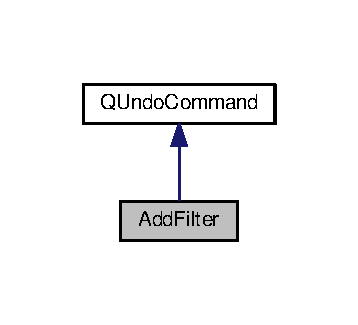
\includegraphics[width=172pt]{classUndoRedo_1_1AddFilter__inherit__graph}
\end{center}
\end{figure}
\subsection*{Public Member Functions}
\begin{DoxyCompactItemize}
\item 
\hyperlink{classUndoRedo_1_1AddFilter_a5a59ac8760928a47325c5d9722ca88cd}{Add\+Filter} (Model\+::\+Filter\+::\+Filter\+Tab $\ast$\hyperlink{classUndoRedo_1_1AddFilter_a47ca82534a740774d79998759818d9f4}{filter\+Tab}, \hyperlink{classModel_1_1Filter}{Model\+::\+Filter} \hyperlink{classUndoRedo_1_1AddFilter_a573678d67a3af0d81b06a4bb3a88957e}{filter})
\item 
void \hyperlink{classUndoRedo_1_1AddFilter_a0e1e7804a53f6d62efc72c9bdbec8571}{undo} ()
\item 
void \hyperlink{classUndoRedo_1_1AddFilter_a93c48d6ed036e1a381be53ac67643284}{redo} ()
\end{DoxyCompactItemize}
\subsection*{Private Attributes}
\begin{DoxyCompactItemize}
\item 
\hyperlink{classGUI_1_1FilterTab}{G\+U\+I\+::\+Filter\+Tab} $\ast$ \hyperlink{classUndoRedo_1_1AddFilter_a47ca82534a740774d79998759818d9f4}{filter\+Tab}
\item 
\hyperlink{classModel_1_1Filter}{Model\+::\+Filter} $\ast$ \hyperlink{classUndoRedo_1_1AddFilter_a573678d67a3af0d81b06a4bb3a88957e}{filter}
\end{DoxyCompactItemize}


\subsection{Detailed Description}
This is the undo command for adding a filter to the filterlist on the filtertab. 

\subsection{Constructor \& Destructor Documentation}
\hypertarget{classUndoRedo_1_1AddFilter_a5a59ac8760928a47325c5d9722ca88cd}{}\index{Undo\+Redo\+::\+Add\+Filter@{Undo\+Redo\+::\+Add\+Filter}!Add\+Filter@{Add\+Filter}}
\index{Add\+Filter@{Add\+Filter}!Undo\+Redo\+::\+Add\+Filter@{Undo\+Redo\+::\+Add\+Filter}}
\subsubsection[{Add\+Filter}]{\setlength{\rightskip}{0pt plus 5cm}{\bf Add\+Filter} (
\begin{DoxyParamCaption}
\item[{Model\+::\+Filter\+::\+Filter\+Tab $\ast$}]{filter\+Tab, }
\item[{{\bf Model\+::\+Filter}}]{filter}
\end{DoxyParamCaption}
)}\label{classUndoRedo_1_1AddFilter_a5a59ac8760928a47325c5d9722ca88cd}


Constructor. 


\begin{DoxyParams}{Parameters}
{\em filter\+Tab} & The filtertab to operate on.\\
\hline
{\em filter} & The filter on which the operation is performed on.\\
\hline
\end{DoxyParams}


\subsection{Member Function Documentation}
\hypertarget{classUndoRedo_1_1AddFilter_a93c48d6ed036e1a381be53ac67643284}{}\index{Undo\+Redo\+::\+Add\+Filter@{Undo\+Redo\+::\+Add\+Filter}!redo@{redo}}
\index{redo@{redo}!Undo\+Redo\+::\+Add\+Filter@{Undo\+Redo\+::\+Add\+Filter}}
\subsubsection[{redo}]{\setlength{\rightskip}{0pt plus 5cm}void redo (
\begin{DoxyParamCaption}
{}
\end{DoxyParamCaption}
)}\label{classUndoRedo_1_1AddFilter_a93c48d6ed036e1a381be53ac67643284}


Adds a filter to the filterlist. 

\hypertarget{classUndoRedo_1_1AddFilter_a0e1e7804a53f6d62efc72c9bdbec8571}{}\index{Undo\+Redo\+::\+Add\+Filter@{Undo\+Redo\+::\+Add\+Filter}!undo@{undo}}
\index{undo@{undo}!Undo\+Redo\+::\+Add\+Filter@{Undo\+Redo\+::\+Add\+Filter}}
\subsubsection[{undo}]{\setlength{\rightskip}{0pt plus 5cm}void undo (
\begin{DoxyParamCaption}
{}
\end{DoxyParamCaption}
)}\label{classUndoRedo_1_1AddFilter_a0e1e7804a53f6d62efc72c9bdbec8571}


Removes the added filter from the filterlist. 



\subsection{Field Documentation}
\hypertarget{classUndoRedo_1_1AddFilter_a573678d67a3af0d81b06a4bb3a88957e}{}\index{Undo\+Redo\+::\+Add\+Filter@{Undo\+Redo\+::\+Add\+Filter}!filter@{filter}}
\index{filter@{filter}!Undo\+Redo\+::\+Add\+Filter@{Undo\+Redo\+::\+Add\+Filter}}
\subsubsection[{filter}]{\setlength{\rightskip}{0pt plus 5cm}{\bf Model\+::\+Filter}$\ast$ filter\hspace{0.3cm}{\ttfamily [private]}}\label{classUndoRedo_1_1AddFilter_a573678d67a3af0d81b06a4bb3a88957e}
\hypertarget{classUndoRedo_1_1AddFilter_a47ca82534a740774d79998759818d9f4}{}\index{Undo\+Redo\+::\+Add\+Filter@{Undo\+Redo\+::\+Add\+Filter}!filter\+Tab@{filter\+Tab}}
\index{filter\+Tab@{filter\+Tab}!Undo\+Redo\+::\+Add\+Filter@{Undo\+Redo\+::\+Add\+Filter}}
\subsubsection[{filter\+Tab}]{\setlength{\rightskip}{0pt plus 5cm}{\bf G\+U\+I\+::\+Filter\+Tab}$\ast$ filter\+Tab\hspace{0.3cm}{\ttfamily [private]}}\label{classUndoRedo_1_1AddFilter_a47ca82534a740774d79998759818d9f4}

\newpage\hypertarget{classUndoRedo_1_1AddVideo}{}\section{Add\+Video Class Reference}
\label{classUndoRedo_1_1AddVideo}\index{Add\+Video@{Add\+Video}}


Inheritance diagram for Add\+Video\+:
\nopagebreak
\begin{figure}[H]
\begin{center}
\leavevmode
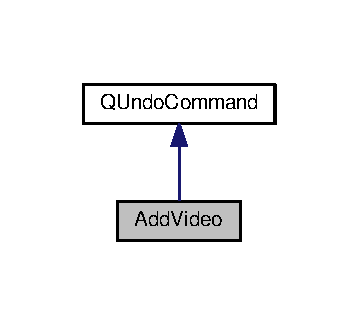
\includegraphics[width=172pt]{classUndoRedo_1_1AddVideo__inherit__graph}
\end{center}
\end{figure}
\subsection*{Public Member Functions}
\begin{DoxyCompactItemize}
\item 
\hyperlink{classUndoRedo_1_1AddVideo_a3725967509af3a267046289fec1c8ad2}{Add\+Video} (\hyperlink{classGUI_1_1AnalysisBoxContainer}{G\+U\+I\+::\+Analysis\+Box\+Container} $\ast$analysis\+Box\+Container, \hyperlink{classModel_1_1EncodedVideo}{Model\+::\+Encoded\+Video} \hyperlink{classUndoRedo_1_1AddVideo_a226620d1252c162814ca98d3e522255c}{video})
\item 
void \hyperlink{classUndoRedo_1_1AddVideo_a0e1e7804a53f6d62efc72c9bdbec8571}{undo} ()
\item 
void \hyperlink{classUndoRedo_1_1AddVideo_a93c48d6ed036e1a381be53ac67643284}{redo} ()
\end{DoxyCompactItemize}
\subsection*{Private Attributes}
\begin{DoxyCompactItemize}
\item 
\hyperlink{classGUI_1_1AnalysisBox}{G\+U\+I\+::\+Analysis\+Box} $\ast$ \hyperlink{classUndoRedo_1_1AddVideo_a574e9e2f540b9068b64a7f26cb40b20a}{ana\+Box}
\item 
\hyperlink{classGUI_1_1AnalysisBoxContainer}{G\+U\+I\+::\+Analysis\+Box\+Container} $\ast$ \hyperlink{classUndoRedo_1_1AddVideo_a69c99d1253a1b743455a030de5a733cb}{ana\+Box\+Container}
\item 
\hyperlink{classModel_1_1EncodedVideo}{Model\+::\+Encoded\+Video} $\ast$ \hyperlink{classUndoRedo_1_1AddVideo_a226620d1252c162814ca98d3e522255c}{video}
\end{DoxyCompactItemize}


\subsection{Detailed Description}
This class is the undo command for adding a encoded video on the analysis tab. 

\subsection{Constructor \& Destructor Documentation}
\hypertarget{classUndoRedo_1_1AddVideo_a3725967509af3a267046289fec1c8ad2}{}\index{Undo\+Redo\+::\+Add\+Video@{Undo\+Redo\+::\+Add\+Video}!Add\+Video@{Add\+Video}}
\index{Add\+Video@{Add\+Video}!Undo\+Redo\+::\+Add\+Video@{Undo\+Redo\+::\+Add\+Video}}
\subsubsection[{Add\+Video}]{\setlength{\rightskip}{0pt plus 5cm}{\bf Add\+Video} (
\begin{DoxyParamCaption}
\item[{{\bf G\+U\+I\+::\+Analysis\+Box\+Container} $\ast$}]{analysis\+Box\+Container, }
\item[{{\bf Model\+::\+Encoded\+Video}}]{video}
\end{DoxyParamCaption}
)}\label{classUndoRedo_1_1AddVideo_a3725967509af3a267046289fec1c8ad2}


Constuctor. 


\begin{DoxyParams}{Parameters}
{\em analysis\+Box\+Container} & The Analysis\+Box\+Container to operate on.\\
\hline
{\em video} & The video on which the action is performed.\\
\hline
\end{DoxyParams}


\subsection{Member Function Documentation}
\hypertarget{classUndoRedo_1_1AddVideo_a93c48d6ed036e1a381be53ac67643284}{}\index{Undo\+Redo\+::\+Add\+Video@{Undo\+Redo\+::\+Add\+Video}!redo@{redo}}
\index{redo@{redo}!Undo\+Redo\+::\+Add\+Video@{Undo\+Redo\+::\+Add\+Video}}
\subsubsection[{redo}]{\setlength{\rightskip}{0pt plus 5cm}void redo (
\begin{DoxyParamCaption}
{}
\end{DoxyParamCaption}
)}\label{classUndoRedo_1_1AddVideo_a93c48d6ed036e1a381be53ac67643284}


Adds a video to the Analysis tab. 

\hypertarget{classUndoRedo_1_1AddVideo_a0e1e7804a53f6d62efc72c9bdbec8571}{}\index{Undo\+Redo\+::\+Add\+Video@{Undo\+Redo\+::\+Add\+Video}!undo@{undo}}
\index{undo@{undo}!Undo\+Redo\+::\+Add\+Video@{Undo\+Redo\+::\+Add\+Video}}
\subsubsection[{undo}]{\setlength{\rightskip}{0pt plus 5cm}void undo (
\begin{DoxyParamCaption}
{}
\end{DoxyParamCaption}
)}\label{classUndoRedo_1_1AddVideo_a0e1e7804a53f6d62efc72c9bdbec8571}


Removes the added video from the analysis tab. 



\subsection{Field Documentation}
\hypertarget{classUndoRedo_1_1AddVideo_a574e9e2f540b9068b64a7f26cb40b20a}{}\index{Undo\+Redo\+::\+Add\+Video@{Undo\+Redo\+::\+Add\+Video}!ana\+Box@{ana\+Box}}
\index{ana\+Box@{ana\+Box}!Undo\+Redo\+::\+Add\+Video@{Undo\+Redo\+::\+Add\+Video}}
\subsubsection[{ana\+Box}]{\setlength{\rightskip}{0pt plus 5cm}{\bf G\+U\+I\+::\+Analysis\+Box}$\ast$ ana\+Box\hspace{0.3cm}{\ttfamily [private]}}\label{classUndoRedo_1_1AddVideo_a574e9e2f540b9068b64a7f26cb40b20a}
\hypertarget{classUndoRedo_1_1AddVideo_a69c99d1253a1b743455a030de5a733cb}{}\index{Undo\+Redo\+::\+Add\+Video@{Undo\+Redo\+::\+Add\+Video}!ana\+Box\+Container@{ana\+Box\+Container}}
\index{ana\+Box\+Container@{ana\+Box\+Container}!Undo\+Redo\+::\+Add\+Video@{Undo\+Redo\+::\+Add\+Video}}
\subsubsection[{ana\+Box\+Container}]{\setlength{\rightskip}{0pt plus 5cm}{\bf G\+U\+I\+::\+Analysis\+Box\+Container}$\ast$ ana\+Box\+Container\hspace{0.3cm}{\ttfamily [private]}}\label{classUndoRedo_1_1AddVideo_a69c99d1253a1b743455a030de5a733cb}
\hypertarget{classUndoRedo_1_1AddVideo_a226620d1252c162814ca98d3e522255c}{}\index{Undo\+Redo\+::\+Add\+Video@{Undo\+Redo\+::\+Add\+Video}!video@{video}}
\index{video@{video}!Undo\+Redo\+::\+Add\+Video@{Undo\+Redo\+::\+Add\+Video}}
\subsubsection[{video}]{\setlength{\rightskip}{0pt plus 5cm}{\bf Model\+::\+Encoded\+Video}$\ast$ video\hspace{0.3cm}{\ttfamily [private]}}\label{classUndoRedo_1_1AddVideo_a226620d1252c162814ca98d3e522255c}

\newpage\hypertarget{classGUI_1_1AnalysisBox}{}\section{Analysis\+Box Class Reference}
\label{classGUI_1_1AnalysisBox}\index{Analysis\+Box@{Analysis\+Box}}
\subsection*{Public Member Functions}
\begin{DoxyCompactItemize}
\item 
\hypertarget{classGUI_1_1AnalysisBox_ae7931451461ed8e1f03a02e7848078c0}{}{\bfseries Analysis\+Box} (\hyperlink{classGUI_1_1QtGui_1_1QWidget____10}{G\+U\+I\+::\+Qt\+Gui\+::\+Q\+Widget\+\_\+\+\_\+10} $\ast$parent)\label{classGUI_1_1AnalysisBox_ae7931451461ed8e1f03a02e7848078c0}

\item 
\hypertarget{classGUI_1_1AnalysisBox_a73fa952c3fb3509d83ca1dadc7cefb33}{}\hyperlink{classMemento_1_1AnalysisBoxMemento}{Memento\+::\+Analysis\+Box\+Memento} {\bfseries get\+Memento} ()\label{classGUI_1_1AnalysisBox_a73fa952c3fb3509d83ca1dadc7cefb33}

\item 
void \hyperlink{classGUI_1_1AnalysisBox_a70c1d51815b73ad12b08cbf0636e77eb}{restore} (\hyperlink{classMemento_1_1AnalysisBoxMemento}{Memento\+::\+Analysis\+Box\+Memento} memento)
\item 
\hypertarget{classGUI_1_1AnalysisBox_a0a63304dda40cabeda44acd79bb08b59}{}void {\bfseries set\+Timer} (shared\+\_\+ptr$<$ \hyperlink{classGUI_1_1Player_1_1Timer}{G\+U\+I\+::\+Player\+::\+Timer} $>$ timer\+:std\+:)\label{classGUI_1_1AnalysisBox_a0a63304dda40cabeda44acd79bb08b59}

\item 
\hypertarget{classGUI_1_1AnalysisBox_ae45e621cb87a85ffb069ac765a306711}{}void {\bfseries set\+Raw\+Video} (\hyperlink{classGUI_1_1Player_1_1Video}{G\+U\+I\+::\+Player\+::\+Video} $\ast$video)\label{classGUI_1_1AnalysisBox_ae45e621cb87a85ffb069ac765a306711}

\item 
\hypertarget{classGUI_1_1AnalysisBox_a9c1b482d1dcd6a733b84a9cdcc960263}{}void {\bfseries set\+Control\+Panel} (Player\+::\+Global\+Control\+Panel $\ast$panel)\label{classGUI_1_1AnalysisBox_a9c1b482d1dcd6a733b84a9cdcc960263}

\item 
\hypertarget{classGUI_1_1AnalysisBox_a9484911b10192b865138995df1158d7e}{}void {\bfseries show\+Macro\+Block\+Video} ()\label{classGUI_1_1AnalysisBox_a9484911b10192b865138995df1158d7e}

\item 
\hypertarget{classGUI_1_1AnalysisBox_a17b13bec505d0e1f579bdfa7f691f085}{}void {\bfseries show\+R\+G\+B\+Difference\+Video} ()\label{classGUI_1_1AnalysisBox_a17b13bec505d0e1f579bdfa7f691f085}

\item 
\hypertarget{classGUI_1_1AnalysisBox_af47ec5ca4337db4deb0b9eefed348e25}{}void {\bfseries set\+Analyse\+Video} (Q\+String path)\label{classGUI_1_1AnalysisBox_af47ec5ca4337db4deb0b9eefed348e25}

\end{DoxyCompactItemize}


\subsection{Detailed Description}
Shows the Analysis of a single video 

\subsection{Member Function Documentation}
\hypertarget{classGUI_1_1AnalysisBox_a70c1d51815b73ad12b08cbf0636e77eb}{}\index{G\+U\+I\+::\+Analysis\+Box@{G\+U\+I\+::\+Analysis\+Box}!restore@{restore}}
\index{restore@{restore}!G\+U\+I\+::\+Analysis\+Box@{G\+U\+I\+::\+Analysis\+Box}}
\subsubsection[{restore}]{\setlength{\rightskip}{0pt plus 5cm}void restore (
\begin{DoxyParamCaption}
\item[{{\bf Memento\+::\+Analysis\+Box\+Memento}}]{memento}
\end{DoxyParamCaption}
)}\label{classGUI_1_1AnalysisBox_a70c1d51815b73ad12b08cbf0636e77eb}


Shows the Analysis of a single video 


\newpage\hypertarget{classGUI_1_1AnalysisBoxContainer}{}\section{Analysis\+Box\+Container Class Reference}
\label{classGUI_1_1AnalysisBoxContainer}\index{Analysis\+Box\+Container@{Analysis\+Box\+Container}}


Inheritance diagram for Analysis\+Box\+Container\+:
\nopagebreak
\begin{figure}[H]
\begin{center}
\leavevmode
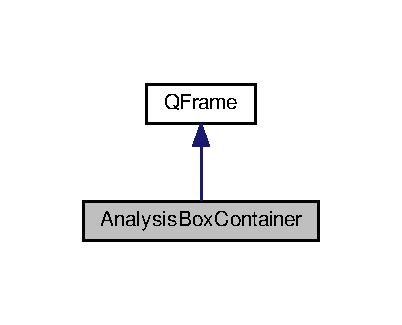
\includegraphics[width=193pt]{classGUI_1_1AnalysisBoxContainer__inherit__graph}
\end{center}
\end{figure}
\subsection*{Public Member Functions}
\begin{DoxyCompactItemize}
\item 
\hyperlink{classGUI_1_1AnalysisBoxContainer_ae603e523cc42100eccf571ff85ca39e8}{Analysis\+Box\+Container} (\hyperlink{classGUI_1_1QWidget}{G\+U\+I\+::\+Q\+Widget} $\ast$parent)
\item 
\hyperlink{classMemento_1_1AnalysisBoxContainerMemento}{Memento\+::\+Analysis\+Box\+Container\+Memento} \hyperlink{classGUI_1_1AnalysisBoxContainer_a0743a7c422123fbd5d22a946af5092ca}{get\+Memento} ()
\item 
void \hyperlink{classGUI_1_1AnalysisBoxContainer_af6d8c35bc3f7000da0579310af42e756}{restore} (\hyperlink{classMemento_1_1AnalysisBoxContainerMemento}{Memento\+::\+Analysis\+Box\+Container\+Memento} memento)
\item 
void \hyperlink{classGUI_1_1AnalysisBoxContainer_af3b761e148d9cb7352c5ffb4bf4c66bd}{add\+Video} (Q\+String path)
\item 
void \hyperlink{classGUI_1_1AnalysisBoxContainer_aa08759618dc05b98d60dc8942d41b556}{set\+Raw\+Video} (\hyperlink{classGUI_1_1Video}{G\+U\+I\+::\+Video} $\ast$video)
\item 
void \hyperlink{classGUI_1_1AnalysisBoxContainer_a678bedcbfc074efd29b5587a753fc341}{set\+Timer} (shared\+\_\+ptr$<$ \hyperlink{classGUI_1_1Timer}{G\+U\+I\+::\+Timer} $>$ timer\+:std\+:)
\item 
void \hyperlink{classGUI_1_1AnalysisBoxContainer_a9c1b482d1dcd6a733b84a9cdcc960263}{set\+Control\+Panel} (Player\+::\+Global\+Control\+Panel $\ast$panel)
\item 
void \hyperlink{classGUI_1_1AnalysisBoxContainer_ab3d9dc42d8e78c5bf6f87c5e93bdf1ce}{show\+Macro\+Block\+Videos} ()
\item 
void \hyperlink{classGUI_1_1AnalysisBoxContainer_a91638333a4b3fe577fd2062f2aa667f3}{show\+R\+G\+B\+Difference\+Videos} ()
\item 
void \hyperlink{classGUI_1_1AnalysisBoxContainer_a181a2114e38722fcae5a9c1d5b1d0ff7}{remove\+Box} (\hyperlink{classGUI_1_1AnalysisBox}{G\+U\+I\+::\+Analysis\+Box} \&box)
\item 
\hyperlink{classGUI_1_1AnalysisBox}{G\+U\+I\+::\+Analysis\+Box} $\ast$ \hyperlink{classGUI_1_1AnalysisBoxContainer_a483776769a5f7b2913128aa76251026b}{add\+Video} (\hyperlink{classModel_1_1EncodedVideo}{Model\+::\+Encoded\+Video} video)
\end{DoxyCompactItemize}
\subsection*{Data Fields}
\begin{DoxyCompactItemize}
\item 
\hyperlink{classUndoRedo_1_1RemoveVideo}{Undo\+Redo\+::\+Remove\+Video} $\ast$ \hyperlink{classGUI_1_1AnalysisBoxContainer_a14b06011d2f6be0da89f067a1e838b09}{ana\+Box\+Container}
\end{DoxyCompactItemize}
\subsection*{Private Attributes}
\begin{DoxyCompactItemize}
\item 
\hyperlink{classGUI_1_1Video}{G\+U\+I\+::\+Video} $\ast$ \hyperlink{classGUI_1_1AnalysisBoxContainer_a36ae288eba0c53b885d93498c8c68469}{raw\+Video}
\item 
shared\+\_\+ptr$<$ \hyperlink{classGUI_1_1Timer}{G\+U\+I\+::\+Timer} $>$ \hyperlink{classGUI_1_1AnalysisBoxContainer_a38f007cbe577c8cecfadf2358a3049fc}{timer}\+:std\+:
\item 
Player\+::\+Global\+Control\+Panel $\ast$ \hyperlink{classGUI_1_1AnalysisBoxContainer_aa7d83e3ba62ee643206acd2a48e058e3}{control\+Panel}
\item 
\hyperlink{classGUI_1_1AnalysisTab}{G\+U\+I\+::\+Analysis\+Tab} $\ast$ \hyperlink{classGUI_1_1AnalysisBoxContainer_a6754830af7090fa0a2bf7c94fbb188cc}{analysis\+Box\+Container}
\item 
std\+::vector$<$ \hyperlink{classGUI_1_1AnalysisBox}{G\+U\+I\+::\+Analysis\+Box} $\ast$ $>$ \hyperlink{classGUI_1_1AnalysisBoxContainer_a5083484e3ec5273e8a150e11fea5108b}{boxes}
\end{DoxyCompactItemize}


\subsection{Detailed Description}
Contains and manages the Analysis\+Boxes. 

\subsection{Constructor \& Destructor Documentation}
\hypertarget{classGUI_1_1AnalysisBoxContainer_ae603e523cc42100eccf571ff85ca39e8}{}\index{G\+U\+I\+::\+Analysis\+Box\+Container@{G\+U\+I\+::\+Analysis\+Box\+Container}!Analysis\+Box\+Container@{Analysis\+Box\+Container}}
\index{Analysis\+Box\+Container@{Analysis\+Box\+Container}!G\+U\+I\+::\+Analysis\+Box\+Container@{G\+U\+I\+::\+Analysis\+Box\+Container}}
\subsubsection[{Analysis\+Box\+Container}]{\setlength{\rightskip}{0pt plus 5cm}{\bf Analysis\+Box\+Container} (
\begin{DoxyParamCaption}
\item[{{\bf G\+U\+I\+::\+Q\+Widget} $\ast$}]{parent}
\end{DoxyParamCaption}
)}\label{classGUI_1_1AnalysisBoxContainer_ae603e523cc42100eccf571ff85ca39e8}


Constructor. 



\subsection{Member Function Documentation}
\hypertarget{classGUI_1_1AnalysisBoxContainer_af3b761e148d9cb7352c5ffb4bf4c66bd}{}\index{G\+U\+I\+::\+Analysis\+Box\+Container@{G\+U\+I\+::\+Analysis\+Box\+Container}!add\+Video@{add\+Video}}
\index{add\+Video@{add\+Video}!G\+U\+I\+::\+Analysis\+Box\+Container@{G\+U\+I\+::\+Analysis\+Box\+Container}}
\subsubsection[{add\+Video}]{\setlength{\rightskip}{0pt plus 5cm}void add\+Video (
\begin{DoxyParamCaption}
\item[{Q\+String}]{path}
\end{DoxyParamCaption}
)}\label{classGUI_1_1AnalysisBoxContainer_af3b761e148d9cb7352c5ffb4bf4c66bd}


Creates a Analysis box and shows it. 


\begin{DoxyParams}{Parameters}
{\em path} & The path of the video to analyse.\\
\hline
\end{DoxyParams}
\hypertarget{classGUI_1_1AnalysisBoxContainer_a483776769a5f7b2913128aa76251026b}{}\index{G\+U\+I\+::\+Analysis\+Box\+Container@{G\+U\+I\+::\+Analysis\+Box\+Container}!add\+Video@{add\+Video}}
\index{add\+Video@{add\+Video}!G\+U\+I\+::\+Analysis\+Box\+Container@{G\+U\+I\+::\+Analysis\+Box\+Container}}
\subsubsection[{add\+Video}]{\setlength{\rightskip}{0pt plus 5cm}{\bf G\+U\+I\+::\+Analysis\+Box}$\ast$ add\+Video (
\begin{DoxyParamCaption}
\item[{{\bf Model\+::\+Encoded\+Video}}]{video}
\end{DoxyParamCaption}
)}\label{classGUI_1_1AnalysisBoxContainer_a483776769a5f7b2913128aa76251026b}


Adds the given video to the container. 


\begin{DoxyParams}{Parameters}
{\em video} & The video to add.\\
\hline
\end{DoxyParams}
\begin{DoxyReturn}{Returns}
The box in which the video is presented.
\end{DoxyReturn}
\hypertarget{classGUI_1_1AnalysisBoxContainer_a0743a7c422123fbd5d22a946af5092ca}{}\index{G\+U\+I\+::\+Analysis\+Box\+Container@{G\+U\+I\+::\+Analysis\+Box\+Container}!get\+Memento@{get\+Memento}}
\index{get\+Memento@{get\+Memento}!G\+U\+I\+::\+Analysis\+Box\+Container@{G\+U\+I\+::\+Analysis\+Box\+Container}}
\subsubsection[{get\+Memento}]{\setlength{\rightskip}{0pt plus 5cm}{\bf Memento\+::\+Analysis\+Box\+Container\+Memento} get\+Memento (
\begin{DoxyParamCaption}
{}
\end{DoxyParamCaption}
)}\label{classGUI_1_1AnalysisBoxContainer_a0743a7c422123fbd5d22a946af5092ca}


Creates a memento which contains the state of the container. 

\begin{DoxyReturn}{Returns}
The created memento.
\end{DoxyReturn}
\hypertarget{classGUI_1_1AnalysisBoxContainer_a181a2114e38722fcae5a9c1d5b1d0ff7}{}\index{G\+U\+I\+::\+Analysis\+Box\+Container@{G\+U\+I\+::\+Analysis\+Box\+Container}!remove\+Box@{remove\+Box}}
\index{remove\+Box@{remove\+Box}!G\+U\+I\+::\+Analysis\+Box\+Container@{G\+U\+I\+::\+Analysis\+Box\+Container}}
\subsubsection[{remove\+Box}]{\setlength{\rightskip}{0pt plus 5cm}void remove\+Box (
\begin{DoxyParamCaption}
\item[{{\bf G\+U\+I\+::\+Analysis\+Box} \&}]{box}
\end{DoxyParamCaption}
)}\label{classGUI_1_1AnalysisBoxContainer_a181a2114e38722fcae5a9c1d5b1d0ff7}


Removes a box from the list. 


\begin{DoxyParams}{Parameters}
{\em box} & The box to remove.\\
\hline
\end{DoxyParams}
\hypertarget{classGUI_1_1AnalysisBoxContainer_af6d8c35bc3f7000da0579310af42e756}{}\index{G\+U\+I\+::\+Analysis\+Box\+Container@{G\+U\+I\+::\+Analysis\+Box\+Container}!restore@{restore}}
\index{restore@{restore}!G\+U\+I\+::\+Analysis\+Box\+Container@{G\+U\+I\+::\+Analysis\+Box\+Container}}
\subsubsection[{restore}]{\setlength{\rightskip}{0pt plus 5cm}void restore (
\begin{DoxyParamCaption}
\item[{{\bf Memento\+::\+Analysis\+Box\+Container\+Memento}}]{memento}
\end{DoxyParamCaption}
)}\label{classGUI_1_1AnalysisBoxContainer_af6d8c35bc3f7000da0579310af42e756}


Restores the container based on the memento. 


\begin{DoxyParams}{Parameters}
{\em memento} & The memento which contains the state to restore.\\
\hline
\end{DoxyParams}
\hypertarget{classGUI_1_1AnalysisBoxContainer_a9c1b482d1dcd6a733b84a9cdcc960263}{}\index{G\+U\+I\+::\+Analysis\+Box\+Container@{G\+U\+I\+::\+Analysis\+Box\+Container}!set\+Control\+Panel@{set\+Control\+Panel}}
\index{set\+Control\+Panel@{set\+Control\+Panel}!G\+U\+I\+::\+Analysis\+Box\+Container@{G\+U\+I\+::\+Analysis\+Box\+Container}}
\subsubsection[{set\+Control\+Panel}]{\setlength{\rightskip}{0pt plus 5cm}void set\+Control\+Panel (
\begin{DoxyParamCaption}
\item[{Player\+::\+Global\+Control\+Panel $\ast$}]{panel}
\end{DoxyParamCaption}
)}\label{classGUI_1_1AnalysisBoxContainer_a9c1b482d1dcd6a733b84a9cdcc960263}


Sets the \hyperlink{classGUI_1_1GlobalControlPanel}{Global\+Control\+Panel}. 


\begin{DoxyParams}{Parameters}
{\em panel} & The panel.\\
\hline
\end{DoxyParams}
\hypertarget{classGUI_1_1AnalysisBoxContainer_aa08759618dc05b98d60dc8942d41b556}{}\index{G\+U\+I\+::\+Analysis\+Box\+Container@{G\+U\+I\+::\+Analysis\+Box\+Container}!set\+Raw\+Video@{set\+Raw\+Video}}
\index{set\+Raw\+Video@{set\+Raw\+Video}!G\+U\+I\+::\+Analysis\+Box\+Container@{G\+U\+I\+::\+Analysis\+Box\+Container}}
\subsubsection[{set\+Raw\+Video}]{\setlength{\rightskip}{0pt plus 5cm}void set\+Raw\+Video (
\begin{DoxyParamCaption}
\item[{{\bf G\+U\+I\+::\+Video} $\ast$}]{video}
\end{DoxyParamCaption}
)}\label{classGUI_1_1AnalysisBoxContainer_aa08759618dc05b98d60dc8942d41b556}


Sets the raw\+Video the encoded videos are compared to. 


\begin{DoxyParams}{Parameters}
{\em video} & The raw video.\\
\hline
\end{DoxyParams}
\hypertarget{classGUI_1_1AnalysisBoxContainer_a678bedcbfc074efd29b5587a753fc341}{}\index{G\+U\+I\+::\+Analysis\+Box\+Container@{G\+U\+I\+::\+Analysis\+Box\+Container}!set\+Timer@{set\+Timer}}
\index{set\+Timer@{set\+Timer}!G\+U\+I\+::\+Analysis\+Box\+Container@{G\+U\+I\+::\+Analysis\+Box\+Container}}
\subsubsection[{set\+Timer}]{\setlength{\rightskip}{0pt plus 5cm}void set\+Timer (
\begin{DoxyParamCaption}
\item[{shared\+\_\+ptr$<$ {\bf G\+U\+I\+::\+Timer} $>$ timer\+:std\+:}]{}
\end{DoxyParamCaption}
)}\label{classGUI_1_1AnalysisBoxContainer_a678bedcbfc074efd29b5587a753fc341}


Sets the timer for the videoplayers. 


\begin{DoxyParams}{Parameters}
{\em timer\+:std,\+:} & The timer for the videoplayers.\\
\hline
\end{DoxyParams}
\hypertarget{classGUI_1_1AnalysisBoxContainer_ab3d9dc42d8e78c5bf6f87c5e93bdf1ce}{}\index{G\+U\+I\+::\+Analysis\+Box\+Container@{G\+U\+I\+::\+Analysis\+Box\+Container}!show\+Macro\+Block\+Videos@{show\+Macro\+Block\+Videos}}
\index{show\+Macro\+Block\+Videos@{show\+Macro\+Block\+Videos}!G\+U\+I\+::\+Analysis\+Box\+Container@{G\+U\+I\+::\+Analysis\+Box\+Container}}
\subsubsection[{show\+Macro\+Block\+Videos}]{\setlength{\rightskip}{0pt plus 5cm}void show\+Macro\+Block\+Videos (
\begin{DoxyParamCaption}
{}
\end{DoxyParamCaption}
)}\label{classGUI_1_1AnalysisBoxContainer_ab3d9dc42d8e78c5bf6f87c5e93bdf1ce}


Tells all Analysis\+Boxes to show the macro block video. 

\hypertarget{classGUI_1_1AnalysisBoxContainer_a91638333a4b3fe577fd2062f2aa667f3}{}\index{G\+U\+I\+::\+Analysis\+Box\+Container@{G\+U\+I\+::\+Analysis\+Box\+Container}!show\+R\+G\+B\+Difference\+Videos@{show\+R\+G\+B\+Difference\+Videos}}
\index{show\+R\+G\+B\+Difference\+Videos@{show\+R\+G\+B\+Difference\+Videos}!G\+U\+I\+::\+Analysis\+Box\+Container@{G\+U\+I\+::\+Analysis\+Box\+Container}}
\subsubsection[{show\+R\+G\+B\+Difference\+Videos}]{\setlength{\rightskip}{0pt plus 5cm}void show\+R\+G\+B\+Difference\+Videos (
\begin{DoxyParamCaption}
{}
\end{DoxyParamCaption}
)}\label{classGUI_1_1AnalysisBoxContainer_a91638333a4b3fe577fd2062f2aa667f3}


Tells all Analysis\+Boxes to show the R\+G\+B\+Diff video. 



\subsection{Field Documentation}
\hypertarget{classGUI_1_1AnalysisBoxContainer_a14b06011d2f6be0da89f067a1e838b09}{}\index{G\+U\+I\+::\+Analysis\+Box\+Container@{G\+U\+I\+::\+Analysis\+Box\+Container}!ana\+Box\+Container@{ana\+Box\+Container}}
\index{ana\+Box\+Container@{ana\+Box\+Container}!G\+U\+I\+::\+Analysis\+Box\+Container@{G\+U\+I\+::\+Analysis\+Box\+Container}}
\subsubsection[{ana\+Box\+Container}]{\setlength{\rightskip}{0pt plus 5cm}{\bf Undo\+Redo\+::\+Remove\+Video}$\ast$ ana\+Box\+Container}\label{classGUI_1_1AnalysisBoxContainer_a14b06011d2f6be0da89f067a1e838b09}
\hypertarget{classGUI_1_1AnalysisBoxContainer_a6754830af7090fa0a2bf7c94fbb188cc}{}\index{G\+U\+I\+::\+Analysis\+Box\+Container@{G\+U\+I\+::\+Analysis\+Box\+Container}!analysis\+Box\+Container@{analysis\+Box\+Container}}
\index{analysis\+Box\+Container@{analysis\+Box\+Container}!G\+U\+I\+::\+Analysis\+Box\+Container@{G\+U\+I\+::\+Analysis\+Box\+Container}}
\subsubsection[{analysis\+Box\+Container}]{\setlength{\rightskip}{0pt plus 5cm}{\bf G\+U\+I\+::\+Analysis\+Tab}$\ast$ analysis\+Box\+Container\hspace{0.3cm}{\ttfamily [private]}}\label{classGUI_1_1AnalysisBoxContainer_a6754830af7090fa0a2bf7c94fbb188cc}
\hypertarget{classGUI_1_1AnalysisBoxContainer_a5083484e3ec5273e8a150e11fea5108b}{}\index{G\+U\+I\+::\+Analysis\+Box\+Container@{G\+U\+I\+::\+Analysis\+Box\+Container}!boxes@{boxes}}
\index{boxes@{boxes}!G\+U\+I\+::\+Analysis\+Box\+Container@{G\+U\+I\+::\+Analysis\+Box\+Container}}
\subsubsection[{boxes}]{\setlength{\rightskip}{0pt plus 5cm}std\+::vector$<${\bf G\+U\+I\+::\+Analysis\+Box}$\ast$$>$ boxes\hspace{0.3cm}{\ttfamily [private]}}\label{classGUI_1_1AnalysisBoxContainer_a5083484e3ec5273e8a150e11fea5108b}
\hypertarget{classGUI_1_1AnalysisBoxContainer_aa7d83e3ba62ee643206acd2a48e058e3}{}\index{G\+U\+I\+::\+Analysis\+Box\+Container@{G\+U\+I\+::\+Analysis\+Box\+Container}!control\+Panel@{control\+Panel}}
\index{control\+Panel@{control\+Panel}!G\+U\+I\+::\+Analysis\+Box\+Container@{G\+U\+I\+::\+Analysis\+Box\+Container}}
\subsubsection[{control\+Panel}]{\setlength{\rightskip}{0pt plus 5cm}Player\+::\+Global\+Control\+Panel$\ast$ control\+Panel\hspace{0.3cm}{\ttfamily [private]}}\label{classGUI_1_1AnalysisBoxContainer_aa7d83e3ba62ee643206acd2a48e058e3}
\hypertarget{classGUI_1_1AnalysisBoxContainer_a36ae288eba0c53b885d93498c8c68469}{}\index{G\+U\+I\+::\+Analysis\+Box\+Container@{G\+U\+I\+::\+Analysis\+Box\+Container}!raw\+Video@{raw\+Video}}
\index{raw\+Video@{raw\+Video}!G\+U\+I\+::\+Analysis\+Box\+Container@{G\+U\+I\+::\+Analysis\+Box\+Container}}
\subsubsection[{raw\+Video}]{\setlength{\rightskip}{0pt plus 5cm}{\bf G\+U\+I\+::\+Video}$\ast$ raw\+Video\hspace{0.3cm}{\ttfamily [private]}}\label{classGUI_1_1AnalysisBoxContainer_a36ae288eba0c53b885d93498c8c68469}
\hypertarget{classGUI_1_1AnalysisBoxContainer_a38f007cbe577c8cecfadf2358a3049fc}{}\index{G\+U\+I\+::\+Analysis\+Box\+Container@{G\+U\+I\+::\+Analysis\+Box\+Container}!timer@{timer}}
\index{timer@{timer}!G\+U\+I\+::\+Analysis\+Box\+Container@{G\+U\+I\+::\+Analysis\+Box\+Container}}
\subsubsection[{timer}]{\setlength{\rightskip}{0pt plus 5cm}shared\+\_\+ptr$<${\bf G\+U\+I\+::\+Timer}$>$ timer\hspace{0.3cm}{\ttfamily [private]}}\label{classGUI_1_1AnalysisBoxContainer_a38f007cbe577c8cecfadf2358a3049fc}

\newpage\hypertarget{classMemento_1_1AnalysisBoxContainerMemento}{}\section{Analysis\+Box\+Container\+Memento Class Reference}
\label{classMemento_1_1AnalysisBoxContainerMemento}\index{Analysis\+Box\+Container\+Memento@{Analysis\+Box\+Container\+Memento}}
\subsection*{Public Member Functions}
\begin{DoxyCompactItemize}
\item 
void \hyperlink{classMemento_1_1AnalysisBoxContainerMemento_a93c3e248eed6b6359984e54bdc3a560d}{analyse\+Box\+Memento} ()
\item 
vector$<$ \hyperlink{classMemento_1_1AnalysisBoxMemento}{Memento\+::\+Analysis\+Box\+Memento} $>$ \hyperlink{classMemento_1_1AnalysisBoxContainerMemento_a8b5776381bcb34875736a6436e848112}{get\+Analysis\+Box\+List} ()
\item 
void \hyperlink{classMemento_1_1AnalysisBoxContainerMemento_a1584f5be1afbee957c6a9a33dc4a6317}{set\+Analysis\+Box\+List} (vector$<$ \hyperlink{classMemento_1_1AnalysisBoxMemento}{Memento\+::\+Analysis\+Box\+Memento} $>$ analyse\+Box\+List\+:std\+:)
\end{DoxyCompactItemize}


\subsection{Detailed Description}
This class is the memento for the Analysis\+Box\+Container. 

\subsection{Member Function Documentation}
\hypertarget{classMemento_1_1AnalysisBoxContainerMemento_a93c3e248eed6b6359984e54bdc3a560d}{}\index{Memento\+::\+Analysis\+Box\+Container\+Memento@{Memento\+::\+Analysis\+Box\+Container\+Memento}!analyse\+Box\+Memento@{analyse\+Box\+Memento}}
\index{analyse\+Box\+Memento@{analyse\+Box\+Memento}!Memento\+::\+Analysis\+Box\+Container\+Memento@{Memento\+::\+Analysis\+Box\+Container\+Memento}}
\subsubsection[{analyse\+Box\+Memento}]{\setlength{\rightskip}{0pt plus 5cm}void analyse\+Box\+Memento (
\begin{DoxyParamCaption}
{}
\end{DoxyParamCaption}
)}\label{classMemento_1_1AnalysisBoxContainerMemento_a93c3e248eed6b6359984e54bdc3a560d}


Constructor. 

\hypertarget{classMemento_1_1AnalysisBoxContainerMemento_a8b5776381bcb34875736a6436e848112}{}\index{Memento\+::\+Analysis\+Box\+Container\+Memento@{Memento\+::\+Analysis\+Box\+Container\+Memento}!get\+Analysis\+Box\+List@{get\+Analysis\+Box\+List}}
\index{get\+Analysis\+Box\+List@{get\+Analysis\+Box\+List}!Memento\+::\+Analysis\+Box\+Container\+Memento@{Memento\+::\+Analysis\+Box\+Container\+Memento}}
\subsubsection[{get\+Analysis\+Box\+List}]{\setlength{\rightskip}{0pt plus 5cm}vector$<$ {\bf Memento\+::\+Analysis\+Box\+Memento} $>$ get\+Analysis\+Box\+List (
\begin{DoxyParamCaption}
{}
\end{DoxyParamCaption}
)}\label{classMemento_1_1AnalysisBoxContainerMemento_a8b5776381bcb34875736a6436e848112}


Returns a list of Analysis\+Box mementos. 

\begin{DoxyReturn}{Returns}
a lists of \hyperlink{classMemento_1_1AnalysisBoxMemento}{Analysis\+Box\+Memento}
\end{DoxyReturn}
\hypertarget{classMemento_1_1AnalysisBoxContainerMemento_a1584f5be1afbee957c6a9a33dc4a6317}{}\index{Memento\+::\+Analysis\+Box\+Container\+Memento@{Memento\+::\+Analysis\+Box\+Container\+Memento}!set\+Analysis\+Box\+List@{set\+Analysis\+Box\+List}}
\index{set\+Analysis\+Box\+List@{set\+Analysis\+Box\+List}!Memento\+::\+Analysis\+Box\+Container\+Memento@{Memento\+::\+Analysis\+Box\+Container\+Memento}}
\subsubsection[{set\+Analysis\+Box\+List}]{\setlength{\rightskip}{0pt plus 5cm}void set\+Analysis\+Box\+List (
\begin{DoxyParamCaption}
\item[{vector$<$ {\bf Memento\+::\+Analysis\+Box\+Memento} $>$ analyse\+Box\+List\+:std\+:}]{}
\end{DoxyParamCaption}
)}\label{classMemento_1_1AnalysisBoxContainerMemento_a1584f5be1afbee957c6a9a33dc4a6317}


Sets the list of \hyperlink{classMemento_1_1AnalysisBoxMemento}{Analysis\+Box\+Memento} 


\begin{DoxyParams}{Parameters}
{\em analyse\+Box\+List\+:std,\+:} & the list of the mementos\\
\hline
\end{DoxyParams}

\newpage\hypertarget{classMemento_1_1AnalysisBoxMemento}{}\section{Analysis\+Box\+Memento Class Reference}
\label{classMemento_1_1AnalysisBoxMemento}\index{Analysis\+Box\+Memento@{Analysis\+Box\+Memento}}
\subsection*{Public Member Functions}
\begin{DoxyCompactItemize}
\item 
\hyperlink{classMemento_1_1AnalysisBoxMemento_a2891757dd897d8d7e04f6ac721863e30}{Analysis\+Box\+Memento} ()
\item 
Q\+String \hyperlink{classMemento_1_1AnalysisBoxMemento_a0aee21e65efbd5059679492dcb847281}{get\+Video\+Path} ()
\item 
void \hyperlink{classMemento_1_1AnalysisBoxMemento_a3db0ccff589bc23a3226a0ac59857437}{set\+Video\+Path} (Q\+String video\+Path)
\item 
Q\+String \hyperlink{classMemento_1_1AnalysisBoxMemento_a8475ee6c96bf1157aa07530f9100416c}{get\+Comment} ()
\item 
void \hyperlink{classMemento_1_1AnalysisBoxMemento_ab3a897eff60f58840c8d1b40292cf047}{set\+Comment} (Q\+String comment)
\item 
\hyperlink{classGUI_1_1Player_1_1Video}{G\+U\+I\+::\+Player\+::\+Video} $\ast$ \hyperlink{classMemento_1_1AnalysisBoxMemento_a4766ee11b86f10503824b3dc18ec3a6d}{get\+Macro\+Video} ()
\item 
void \hyperlink{classMemento_1_1AnalysisBoxMemento_ab43a2220425e3311fa978cebe61db3e4}{set\+Macro\+Video} (\hyperlink{classGUI_1_1Player_1_1Video}{G\+U\+I\+::\+Player\+::\+Video} $\ast$macro\+Video)
\item 
\hyperlink{classGUI_1_1Player_1_1Video}{G\+U\+I\+::\+Player\+::\+Video} $\ast$ \hyperlink{classMemento_1_1AnalysisBoxMemento_aeafaf51d6b8da8f5015d7887cf00c474}{get\+Rgb\+Diff\+Video} ()
\item 
void \hyperlink{classMemento_1_1AnalysisBoxMemento_a15413d63ffb3c5f97f39d3c2f11b5c0e}{set\+Rgb\+Diff\+Video} (\hyperlink{classGUI_1_1Player_1_1Video}{G\+U\+I\+::\+Player\+::\+Video} $\ast$rgb\+Diff\+Video)
\item 
Q\+Image \hyperlink{classMemento_1_1AnalysisBoxMemento_a581aa3ebb51a9ce69dcbe21d6f949e99}{get\+Psnr} ()
\item 
void \hyperlink{classMemento_1_1AnalysisBoxMemento_a5613ac52b106bb5859856712c3a3279f}{set\+Psnr} (Q\+Image psnr)
\item 
Q\+Image \hyperlink{classMemento_1_1AnalysisBoxMemento_a0b8e4c45925b9a6f85c327561d7a4369}{get\+Bitrate} ()
\item 
void \hyperlink{classMemento_1_1AnalysisBoxMemento_ad755ae317fc096de20872b5daf21d69d}{set\+Bitrate} (Q\+Image bitrate)
\end{DoxyCompactItemize}


\subsection{Detailed Description}
This class is the memento for the Analysis\+Box. 

\subsection{Constructor \& Destructor Documentation}
\hypertarget{classMemento_1_1AnalysisBoxMemento_a2891757dd897d8d7e04f6ac721863e30}{}\index{Memento\+::\+Analysis\+Box\+Memento@{Memento\+::\+Analysis\+Box\+Memento}!Analysis\+Box\+Memento@{Analysis\+Box\+Memento}}
\index{Analysis\+Box\+Memento@{Analysis\+Box\+Memento}!Memento\+::\+Analysis\+Box\+Memento@{Memento\+::\+Analysis\+Box\+Memento}}
\subsubsection[{Analysis\+Box\+Memento}]{\setlength{\rightskip}{0pt plus 5cm}{\bf Analysis\+Box\+Memento} (
\begin{DoxyParamCaption}
{}
\end{DoxyParamCaption}
)}\label{classMemento_1_1AnalysisBoxMemento_a2891757dd897d8d7e04f6ac721863e30}


Constrictor. 



\subsection{Member Function Documentation}
\hypertarget{classMemento_1_1AnalysisBoxMemento_a0b8e4c45925b9a6f85c327561d7a4369}{}\index{Memento\+::\+Analysis\+Box\+Memento@{Memento\+::\+Analysis\+Box\+Memento}!get\+Bitrate@{get\+Bitrate}}
\index{get\+Bitrate@{get\+Bitrate}!Memento\+::\+Analysis\+Box\+Memento@{Memento\+::\+Analysis\+Box\+Memento}}
\subsubsection[{get\+Bitrate}]{\setlength{\rightskip}{0pt plus 5cm}Q\+Image get\+Bitrate (
\begin{DoxyParamCaption}
{}
\end{DoxyParamCaption}
)}\label{classMemento_1_1AnalysisBoxMemento_a0b8e4c45925b9a6f85c327561d7a4369}


Returns an image of the bitrate graph. 

\begin{DoxyReturn}{Returns}
an image of the bitrate graph
\end{DoxyReturn}
\hypertarget{classMemento_1_1AnalysisBoxMemento_a8475ee6c96bf1157aa07530f9100416c}{}\index{Memento\+::\+Analysis\+Box\+Memento@{Memento\+::\+Analysis\+Box\+Memento}!get\+Comment@{get\+Comment}}
\index{get\+Comment@{get\+Comment}!Memento\+::\+Analysis\+Box\+Memento@{Memento\+::\+Analysis\+Box\+Memento}}
\subsubsection[{get\+Comment}]{\setlength{\rightskip}{0pt plus 5cm}Q\+String get\+Comment (
\begin{DoxyParamCaption}
{}
\end{DoxyParamCaption}
)}\label{classMemento_1_1AnalysisBoxMemento_a8475ee6c96bf1157aa07530f9100416c}


Returns the user comment. 

\begin{DoxyReturn}{Returns}
the user comment
\end{DoxyReturn}
\hypertarget{classMemento_1_1AnalysisBoxMemento_a4766ee11b86f10503824b3dc18ec3a6d}{}\index{Memento\+::\+Analysis\+Box\+Memento@{Memento\+::\+Analysis\+Box\+Memento}!get\+Macro\+Video@{get\+Macro\+Video}}
\index{get\+Macro\+Video@{get\+Macro\+Video}!Memento\+::\+Analysis\+Box\+Memento@{Memento\+::\+Analysis\+Box\+Memento}}
\subsubsection[{get\+Macro\+Video}]{\setlength{\rightskip}{0pt plus 5cm}{\bf G\+U\+I\+::\+Player\+::\+Video} $\ast$ get\+Macro\+Video (
\begin{DoxyParamCaption}
{}
\end{DoxyParamCaption}
)}\label{classMemento_1_1AnalysisBoxMemento_a4766ee11b86f10503824b3dc18ec3a6d}


Returns the macroblock video. 

\begin{DoxyReturn}{Returns}
the macroblock video
\end{DoxyReturn}
\hypertarget{classMemento_1_1AnalysisBoxMemento_a581aa3ebb51a9ce69dcbe21d6f949e99}{}\index{Memento\+::\+Analysis\+Box\+Memento@{Memento\+::\+Analysis\+Box\+Memento}!get\+Psnr@{get\+Psnr}}
\index{get\+Psnr@{get\+Psnr}!Memento\+::\+Analysis\+Box\+Memento@{Memento\+::\+Analysis\+Box\+Memento}}
\subsubsection[{get\+Psnr}]{\setlength{\rightskip}{0pt plus 5cm}Q\+Image get\+Psnr (
\begin{DoxyParamCaption}
{}
\end{DoxyParamCaption}
)}\label{classMemento_1_1AnalysisBoxMemento_a581aa3ebb51a9ce69dcbe21d6f949e99}


Returns an image of the psnr graph. 

\begin{DoxyReturn}{Returns}
an image of the psnr graph
\end{DoxyReturn}
\hypertarget{classMemento_1_1AnalysisBoxMemento_aeafaf51d6b8da8f5015d7887cf00c474}{}\index{Memento\+::\+Analysis\+Box\+Memento@{Memento\+::\+Analysis\+Box\+Memento}!get\+Rgb\+Diff\+Video@{get\+Rgb\+Diff\+Video}}
\index{get\+Rgb\+Diff\+Video@{get\+Rgb\+Diff\+Video}!Memento\+::\+Analysis\+Box\+Memento@{Memento\+::\+Analysis\+Box\+Memento}}
\subsubsection[{get\+Rgb\+Diff\+Video}]{\setlength{\rightskip}{0pt plus 5cm}{\bf G\+U\+I\+::\+Player\+::\+Video} $\ast$ get\+Rgb\+Diff\+Video (
\begin{DoxyParamCaption}
{}
\end{DoxyParamCaption}
)}\label{classMemento_1_1AnalysisBoxMemento_aeafaf51d6b8da8f5015d7887cf00c474}


Returns the rgb difference video. 

\begin{DoxyReturn}{Returns}
the rgb difference video
\end{DoxyReturn}
\hypertarget{classMemento_1_1AnalysisBoxMemento_a0aee21e65efbd5059679492dcb847281}{}\index{Memento\+::\+Analysis\+Box\+Memento@{Memento\+::\+Analysis\+Box\+Memento}!get\+Video\+Path@{get\+Video\+Path}}
\index{get\+Video\+Path@{get\+Video\+Path}!Memento\+::\+Analysis\+Box\+Memento@{Memento\+::\+Analysis\+Box\+Memento}}
\subsubsection[{get\+Video\+Path}]{\setlength{\rightskip}{0pt plus 5cm}Q\+String get\+Video\+Path (
\begin{DoxyParamCaption}
{}
\end{DoxyParamCaption}
)}\label{classMemento_1_1AnalysisBoxMemento_a0aee21e65efbd5059679492dcb847281}


Returns the path to the video. 

\begin{DoxyReturn}{Returns}
absolute path to the video
\end{DoxyReturn}
\hypertarget{classMemento_1_1AnalysisBoxMemento_ad755ae317fc096de20872b5daf21d69d}{}\index{Memento\+::\+Analysis\+Box\+Memento@{Memento\+::\+Analysis\+Box\+Memento}!set\+Bitrate@{set\+Bitrate}}
\index{set\+Bitrate@{set\+Bitrate}!Memento\+::\+Analysis\+Box\+Memento@{Memento\+::\+Analysis\+Box\+Memento}}
\subsubsection[{set\+Bitrate}]{\setlength{\rightskip}{0pt plus 5cm}void set\+Bitrate (
\begin{DoxyParamCaption}
\item[{Q\+Image}]{bitrate}
\end{DoxyParamCaption}
)}\label{classMemento_1_1AnalysisBoxMemento_ad755ae317fc096de20872b5daf21d69d}


Sets the image for the bitrate graph. 


\begin{DoxyParams}{Parameters}
{\em bitrate} & the image of the bitrate gaph\\
\hline
\end{DoxyParams}
\hypertarget{classMemento_1_1AnalysisBoxMemento_ab3a897eff60f58840c8d1b40292cf047}{}\index{Memento\+::\+Analysis\+Box\+Memento@{Memento\+::\+Analysis\+Box\+Memento}!set\+Comment@{set\+Comment}}
\index{set\+Comment@{set\+Comment}!Memento\+::\+Analysis\+Box\+Memento@{Memento\+::\+Analysis\+Box\+Memento}}
\subsubsection[{set\+Comment}]{\setlength{\rightskip}{0pt plus 5cm}void set\+Comment (
\begin{DoxyParamCaption}
\item[{Q\+String}]{comment}
\end{DoxyParamCaption}
)}\label{classMemento_1_1AnalysisBoxMemento_ab3a897eff60f58840c8d1b40292cf047}


Sets the user comment. 


\begin{DoxyParams}{Parameters}
{\em comment} & the user comment\\
\hline
\end{DoxyParams}
\hypertarget{classMemento_1_1AnalysisBoxMemento_ab43a2220425e3311fa978cebe61db3e4}{}\index{Memento\+::\+Analysis\+Box\+Memento@{Memento\+::\+Analysis\+Box\+Memento}!set\+Macro\+Video@{set\+Macro\+Video}}
\index{set\+Macro\+Video@{set\+Macro\+Video}!Memento\+::\+Analysis\+Box\+Memento@{Memento\+::\+Analysis\+Box\+Memento}}
\subsubsection[{set\+Macro\+Video}]{\setlength{\rightskip}{0pt plus 5cm}void set\+Macro\+Video (
\begin{DoxyParamCaption}
\item[{{\bf G\+U\+I\+::\+Player\+::\+Video} $\ast$}]{macro\+Video}
\end{DoxyParamCaption}
)}\label{classMemento_1_1AnalysisBoxMemento_ab43a2220425e3311fa978cebe61db3e4}


Sets the macroblock video. 


\begin{DoxyParams}{Parameters}
{\em macro\+Video} & the macroblock video\\
\hline
\end{DoxyParams}
\hypertarget{classMemento_1_1AnalysisBoxMemento_a5613ac52b106bb5859856712c3a3279f}{}\index{Memento\+::\+Analysis\+Box\+Memento@{Memento\+::\+Analysis\+Box\+Memento}!set\+Psnr@{set\+Psnr}}
\index{set\+Psnr@{set\+Psnr}!Memento\+::\+Analysis\+Box\+Memento@{Memento\+::\+Analysis\+Box\+Memento}}
\subsubsection[{set\+Psnr}]{\setlength{\rightskip}{0pt plus 5cm}void set\+Psnr (
\begin{DoxyParamCaption}
\item[{Q\+Image}]{psnr}
\end{DoxyParamCaption}
)}\label{classMemento_1_1AnalysisBoxMemento_a5613ac52b106bb5859856712c3a3279f}


Sets the image of the psnr graph. 


\begin{DoxyParams}{Parameters}
{\em psnr} & the image of the psnr graph\\
\hline
\end{DoxyParams}
\hypertarget{classMemento_1_1AnalysisBoxMemento_a15413d63ffb3c5f97f39d3c2f11b5c0e}{}\index{Memento\+::\+Analysis\+Box\+Memento@{Memento\+::\+Analysis\+Box\+Memento}!set\+Rgb\+Diff\+Video@{set\+Rgb\+Diff\+Video}}
\index{set\+Rgb\+Diff\+Video@{set\+Rgb\+Diff\+Video}!Memento\+::\+Analysis\+Box\+Memento@{Memento\+::\+Analysis\+Box\+Memento}}
\subsubsection[{set\+Rgb\+Diff\+Video}]{\setlength{\rightskip}{0pt plus 5cm}void set\+Rgb\+Diff\+Video (
\begin{DoxyParamCaption}
\item[{{\bf G\+U\+I\+::\+Player\+::\+Video} $\ast$}]{rgb\+Diff\+Video}
\end{DoxyParamCaption}
)}\label{classMemento_1_1AnalysisBoxMemento_a15413d63ffb3c5f97f39d3c2f11b5c0e}


Sets the rgb difference video. 


\begin{DoxyParams}{Parameters}
{\em rgb\+Diff\+Video} & the rgb difference video\\
\hline
\end{DoxyParams}
\hypertarget{classMemento_1_1AnalysisBoxMemento_a3db0ccff589bc23a3226a0ac59857437}{}\index{Memento\+::\+Analysis\+Box\+Memento@{Memento\+::\+Analysis\+Box\+Memento}!set\+Video\+Path@{set\+Video\+Path}}
\index{set\+Video\+Path@{set\+Video\+Path}!Memento\+::\+Analysis\+Box\+Memento@{Memento\+::\+Analysis\+Box\+Memento}}
\subsubsection[{set\+Video\+Path}]{\setlength{\rightskip}{0pt plus 5cm}void set\+Video\+Path (
\begin{DoxyParamCaption}
\item[{Q\+String}]{video\+Path}
\end{DoxyParamCaption}
)}\label{classMemento_1_1AnalysisBoxMemento_a3db0ccff589bc23a3226a0ac59857437}


Sets the path to the video. 


\begin{DoxyParams}{Parameters}
{\em video\+Path} & absolute path to the video\\
\hline
\end{DoxyParams}

\newpage\hypertarget{classGUI_1_1AnalysisTab}{}\section{Analysis\+Tab Class Reference}
\label{classGUI_1_1AnalysisTab}\index{Analysis\+Tab@{Analysis\+Tab}}
\subsection*{Public Member Functions}
\begin{DoxyCompactItemize}
\item 
\hypertarget{classGUI_1_1AnalysisTab_a544106f19b9119dd044e0b351af6b8a0}{}{\bfseries Analysis\+Tab} (\hyperlink{classGUI_1_1QtGui_1_1QWidget____10}{G\+U\+I\+::\+Qt\+Gui\+::\+Q\+Widget\+\_\+\+\_\+10} $\ast$parent)\label{classGUI_1_1AnalysisTab_a544106f19b9119dd044e0b351af6b8a0}

\item 
\hypertarget{classGUI_1_1AnalysisTab_ad452524ed628a2eba1f167f79469b829}{}\hyperlink{classMemento_1_1AnalysisTabMemento}{Memento\+::\+Analysis\+Tab\+Memento} {\bfseries get\+Memento} ()\label{classGUI_1_1AnalysisTab_ad452524ed628a2eba1f167f79469b829}

\item 
\hypertarget{classGUI_1_1AnalysisTab_a37a387e0b6f67a340ff7e60b2f8f7f24}{}void {\bfseries restore} (\hyperlink{classMemento_1_1AnalysisTabMemento}{Memento\+::\+Analysis\+Tab\+Memento} memento)\label{classGUI_1_1AnalysisTab_a37a387e0b6f67a340ff7e60b2f8f7f24}

\end{DoxyCompactItemize}
\subsection*{Data Fields}
\begin{DoxyCompactItemize}
\item 
\hypertarget{classGUI_1_1AnalysisTab_ad1a5ead95d905d9ec387ee6c95665c38}{}\hyperlink{classGUI_1_1Player_1_1FrameView}{G\+U\+I\+::\+Player\+::\+Frame\+View} $\ast$ {\bfseries raw\+Video\+View}\label{classGUI_1_1AnalysisTab_ad1a5ead95d905d9ec387ee6c95665c38}

\end{DoxyCompactItemize}


\subsection{Detailed Description}
the tab that shows videos and analyses them 
\newpage\hypertarget{classMemento_1_1AnalysisTabMemento}{}\section{Analysis\+Tab\+Memento Class Reference}
\label{classMemento_1_1AnalysisTabMemento}\index{Analysis\+Tab\+Memento@{Analysis\+Tab\+Memento}}
\subsection*{Public Member Functions}
\begin{DoxyCompactItemize}
\item 
\hyperlink{classMemento_1_1AnalysisTabMemento_a035f84d6066cdb7d8a475da4710d2e67}{Analysis\+Tab\+Memento} ()
\item 
int \hyperlink{classMemento_1_1AnalysisTabMemento_af7babc742dcea9250c73c408b2cfacf2}{get\+Current\+Video\+Position} ()
\item 
void \hyperlink{classMemento_1_1AnalysisTabMemento_a66ff926aa567b15381b5906cd65c6b7d}{set\+Current\+Video\+Position} (int current\+Video\+Position)
\item 
int \hyperlink{classMemento_1_1AnalysisTabMemento_a687a0fc92408cf713058eaf23abc22f3}{get\+Currently\+Shown\+Analysis\+Video} ()
\item 
void \hyperlink{classMemento_1_1AnalysisTabMemento_a1d76537f6e47c09e47bf15eefd26feff}{set\+Currently\+Shown\+Analysis\+Video} (int currently\+Shown\+Analysis\+Video)
\item 
float \hyperlink{classMemento_1_1AnalysisTabMemento_a4c7df241ee5989199664bfc3b336d228}{get\+Current\+Speed} ()
\item 
void \hyperlink{classMemento_1_1AnalysisTabMemento_aa99f3e18fe8363d1333c1ddedfa12084}{set\+Current\+Speed} (float current\+Speed)
\item 
\hyperlink{classMemento_1_1AnalysisBoxContainerMemento}{Memento\+::\+Analysis\+Box\+Container\+Memento} \hyperlink{classMemento_1_1AnalysisTabMemento_a1882d53a845bc483ee4974f633026043}{get\+Analysis\+Box\+Container\+Memento} ()
\item 
void \hyperlink{classMemento_1_1AnalysisTabMemento_aca56db151b2ff66e743215ac8bc5b942}{set\+Analysis\+Box\+Container\+Memento} (\hyperlink{classMemento_1_1AnalysisBoxContainerMemento}{Memento\+::\+Analysis\+Box\+Container\+Memento} analysis\+Box\+Container\+Memento)
\end{DoxyCompactItemize}


\subsection{Detailed Description}
This class is the memento for the analysis tab. 

\subsection{Constructor \& Destructor Documentation}
\hypertarget{classMemento_1_1AnalysisTabMemento_a035f84d6066cdb7d8a475da4710d2e67}{}\index{Memento\+::\+Analysis\+Tab\+Memento@{Memento\+::\+Analysis\+Tab\+Memento}!Analysis\+Tab\+Memento@{Analysis\+Tab\+Memento}}
\index{Analysis\+Tab\+Memento@{Analysis\+Tab\+Memento}!Memento\+::\+Analysis\+Tab\+Memento@{Memento\+::\+Analysis\+Tab\+Memento}}
\subsubsection[{Analysis\+Tab\+Memento}]{\setlength{\rightskip}{0pt plus 5cm}{\bf Analysis\+Tab\+Memento} (
\begin{DoxyParamCaption}
{}
\end{DoxyParamCaption}
)}\label{classMemento_1_1AnalysisTabMemento_a035f84d6066cdb7d8a475da4710d2e67}


Constructor. 



\subsection{Member Function Documentation}
\hypertarget{classMemento_1_1AnalysisTabMemento_a1882d53a845bc483ee4974f633026043}{}\index{Memento\+::\+Analysis\+Tab\+Memento@{Memento\+::\+Analysis\+Tab\+Memento}!get\+Analysis\+Box\+Container\+Memento@{get\+Analysis\+Box\+Container\+Memento}}
\index{get\+Analysis\+Box\+Container\+Memento@{get\+Analysis\+Box\+Container\+Memento}!Memento\+::\+Analysis\+Tab\+Memento@{Memento\+::\+Analysis\+Tab\+Memento}}
\subsubsection[{get\+Analysis\+Box\+Container\+Memento}]{\setlength{\rightskip}{0pt plus 5cm}{\bf Memento\+::\+Analysis\+Box\+Container\+Memento} get\+Analysis\+Box\+Container\+Memento (
\begin{DoxyParamCaption}
{}
\end{DoxyParamCaption}
)}\label{classMemento_1_1AnalysisTabMemento_a1882d53a845bc483ee4974f633026043}


Returns the memento of the Analysis\+Box\+Container. 

\begin{DoxyReturn}{Returns}
the memento of the Analysis\+Box\+Container
\end{DoxyReturn}
\hypertarget{classMemento_1_1AnalysisTabMemento_a687a0fc92408cf713058eaf23abc22f3}{}\index{Memento\+::\+Analysis\+Tab\+Memento@{Memento\+::\+Analysis\+Tab\+Memento}!get\+Currently\+Shown\+Analysis\+Video@{get\+Currently\+Shown\+Analysis\+Video}}
\index{get\+Currently\+Shown\+Analysis\+Video@{get\+Currently\+Shown\+Analysis\+Video}!Memento\+::\+Analysis\+Tab\+Memento@{Memento\+::\+Analysis\+Tab\+Memento}}
\subsubsection[{get\+Currently\+Shown\+Analysis\+Video}]{\setlength{\rightskip}{0pt plus 5cm}int get\+Currently\+Shown\+Analysis\+Video (
\begin{DoxyParamCaption}
{}
\end{DoxyParamCaption}
)}\label{classMemento_1_1AnalysisTabMemento_a687a0fc92408cf713058eaf23abc22f3}


Returns what analysis video is currently shown. 0 means rgb difference. non zero means macroblocks. 

\begin{DoxyReturn}{Returns}
the currently shown analysis video
\end{DoxyReturn}
\hypertarget{classMemento_1_1AnalysisTabMemento_a4c7df241ee5989199664bfc3b336d228}{}\index{Memento\+::\+Analysis\+Tab\+Memento@{Memento\+::\+Analysis\+Tab\+Memento}!get\+Current\+Speed@{get\+Current\+Speed}}
\index{get\+Current\+Speed@{get\+Current\+Speed}!Memento\+::\+Analysis\+Tab\+Memento@{Memento\+::\+Analysis\+Tab\+Memento}}
\subsubsection[{get\+Current\+Speed}]{\setlength{\rightskip}{0pt plus 5cm}float get\+Current\+Speed (
\begin{DoxyParamCaption}
{}
\end{DoxyParamCaption}
)}\label{classMemento_1_1AnalysisTabMemento_a4c7df241ee5989199664bfc3b336d228}


Returns the current speed of the player. 

\begin{DoxyReturn}{Returns}
the current speed of the player
\end{DoxyReturn}
\hypertarget{classMemento_1_1AnalysisTabMemento_af7babc742dcea9250c73c408b2cfacf2}{}\index{Memento\+::\+Analysis\+Tab\+Memento@{Memento\+::\+Analysis\+Tab\+Memento}!get\+Current\+Video\+Position@{get\+Current\+Video\+Position}}
\index{get\+Current\+Video\+Position@{get\+Current\+Video\+Position}!Memento\+::\+Analysis\+Tab\+Memento@{Memento\+::\+Analysis\+Tab\+Memento}}
\subsubsection[{get\+Current\+Video\+Position}]{\setlength{\rightskip}{0pt plus 5cm}int get\+Current\+Video\+Position (
\begin{DoxyParamCaption}
{}
\end{DoxyParamCaption}
)}\label{classMemento_1_1AnalysisTabMemento_af7babc742dcea9250c73c408b2cfacf2}


Returns the current position the player is at. 

\begin{DoxyReturn}{Returns}
the current position of the player
\end{DoxyReturn}
\hypertarget{classMemento_1_1AnalysisTabMemento_aca56db151b2ff66e743215ac8bc5b942}{}\index{Memento\+::\+Analysis\+Tab\+Memento@{Memento\+::\+Analysis\+Tab\+Memento}!set\+Analysis\+Box\+Container\+Memento@{set\+Analysis\+Box\+Container\+Memento}}
\index{set\+Analysis\+Box\+Container\+Memento@{set\+Analysis\+Box\+Container\+Memento}!Memento\+::\+Analysis\+Tab\+Memento@{Memento\+::\+Analysis\+Tab\+Memento}}
\subsubsection[{set\+Analysis\+Box\+Container\+Memento}]{\setlength{\rightskip}{0pt plus 5cm}void set\+Analysis\+Box\+Container\+Memento (
\begin{DoxyParamCaption}
\item[{{\bf Memento\+::\+Analysis\+Box\+Container\+Memento}}]{analysis\+Box\+Container\+Memento}
\end{DoxyParamCaption}
)}\label{classMemento_1_1AnalysisTabMemento_aca56db151b2ff66e743215ac8bc5b942}


Sets the memento of the Analysis\+Box\+Container. 


\begin{DoxyParams}{Parameters}
{\em analysis\+Box\+Container\+Memento} & the memento of the Analysis\+Box\+Container\\
\hline
\end{DoxyParams}
\hypertarget{classMemento_1_1AnalysisTabMemento_a1d76537f6e47c09e47bf15eefd26feff}{}\index{Memento\+::\+Analysis\+Tab\+Memento@{Memento\+::\+Analysis\+Tab\+Memento}!set\+Currently\+Shown\+Analysis\+Video@{set\+Currently\+Shown\+Analysis\+Video}}
\index{set\+Currently\+Shown\+Analysis\+Video@{set\+Currently\+Shown\+Analysis\+Video}!Memento\+::\+Analysis\+Tab\+Memento@{Memento\+::\+Analysis\+Tab\+Memento}}
\subsubsection[{set\+Currently\+Shown\+Analysis\+Video}]{\setlength{\rightskip}{0pt plus 5cm}void set\+Currently\+Shown\+Analysis\+Video (
\begin{DoxyParamCaption}
\item[{int}]{currently\+Shown\+Analysis\+Video}
\end{DoxyParamCaption}
)}\label{classMemento_1_1AnalysisTabMemento_a1d76537f6e47c09e47bf15eefd26feff}


Sets the currently shown analysis video. 0 means rgb difference. non 0 means macroblocks. 


\begin{DoxyParams}{Parameters}
{\em currently\+Shown\+Analysis\+Video} & the currrently shown analysis video\\
\hline
\end{DoxyParams}
\hypertarget{classMemento_1_1AnalysisTabMemento_aa99f3e18fe8363d1333c1ddedfa12084}{}\index{Memento\+::\+Analysis\+Tab\+Memento@{Memento\+::\+Analysis\+Tab\+Memento}!set\+Current\+Speed@{set\+Current\+Speed}}
\index{set\+Current\+Speed@{set\+Current\+Speed}!Memento\+::\+Analysis\+Tab\+Memento@{Memento\+::\+Analysis\+Tab\+Memento}}
\subsubsection[{set\+Current\+Speed}]{\setlength{\rightskip}{0pt plus 5cm}void set\+Current\+Speed (
\begin{DoxyParamCaption}
\item[{float}]{current\+Speed}
\end{DoxyParamCaption}
)}\label{classMemento_1_1AnalysisTabMemento_aa99f3e18fe8363d1333c1ddedfa12084}


Sets the current speed of the player. 


\begin{DoxyParams}{Parameters}
{\em current\+Speed} & the current speed of the player\\
\hline
\end{DoxyParams}
\hypertarget{classMemento_1_1AnalysisTabMemento_a66ff926aa567b15381b5906cd65c6b7d}{}\index{Memento\+::\+Analysis\+Tab\+Memento@{Memento\+::\+Analysis\+Tab\+Memento}!set\+Current\+Video\+Position@{set\+Current\+Video\+Position}}
\index{set\+Current\+Video\+Position@{set\+Current\+Video\+Position}!Memento\+::\+Analysis\+Tab\+Memento@{Memento\+::\+Analysis\+Tab\+Memento}}
\subsubsection[{set\+Current\+Video\+Position}]{\setlength{\rightskip}{0pt plus 5cm}void set\+Current\+Video\+Position (
\begin{DoxyParamCaption}
\item[{int}]{current\+Video\+Position}
\end{DoxyParamCaption}
)}\label{classMemento_1_1AnalysisTabMemento_a66ff926aa567b15381b5906cd65c6b7d}


Sets the current position of the player. 


\begin{DoxyParams}{Parameters}
{\em current\+Video\+Position} & the current position of the player\\
\hline
\end{DoxyParams}

\newpage\hypertarget{classUndoRedo_1_1ApplyFilter}{}\section{Apply\+Filter Class Reference}
\label{classUndoRedo_1_1ApplyFilter}\index{Apply\+Filter@{Apply\+Filter}}
\subsection*{Public Member Functions}
\begin{DoxyCompactItemize}
\item 
\hyperlink{classUndoRedo_1_1ApplyFilter_a6ca759bf9a36b367359507b28e0b2459}{Apply\+Filter} (\hyperlink{classGUI_1_1FilterTab}{G\+U\+I\+::\+Filter\+Tab} $\ast$filter\+Tab)
\item 
void \hyperlink{classUndoRedo_1_1ApplyFilter_a0e1e7804a53f6d62efc72c9bdbec8571}{undo} ()
\item 
void \hyperlink{classUndoRedo_1_1ApplyFilter_a93c48d6ed036e1a381be53ac67643284}{redo} ()
\end{DoxyCompactItemize}


\subsection{Detailed Description}
This class is the undo command for applying filters on the filtertab. 

\subsection{Constructor \& Destructor Documentation}
\hypertarget{classUndoRedo_1_1ApplyFilter_a6ca759bf9a36b367359507b28e0b2459}{}\index{Undo\+Redo\+::\+Apply\+Filter@{Undo\+Redo\+::\+Apply\+Filter}!Apply\+Filter@{Apply\+Filter}}
\index{Apply\+Filter@{Apply\+Filter}!Undo\+Redo\+::\+Apply\+Filter@{Undo\+Redo\+::\+Apply\+Filter}}
\subsubsection[{Apply\+Filter}]{\setlength{\rightskip}{0pt plus 5cm}{\bf Apply\+Filter} (
\begin{DoxyParamCaption}
\item[{{\bf G\+U\+I\+::\+Filter\+Tab} $\ast$}]{filter\+Tab}
\end{DoxyParamCaption}
)}\label{classUndoRedo_1_1ApplyFilter_a6ca759bf9a36b367359507b28e0b2459}


Constuctor 



\subsection{Member Function Documentation}
\hypertarget{classUndoRedo_1_1ApplyFilter_a93c48d6ed036e1a381be53ac67643284}{}\index{Undo\+Redo\+::\+Apply\+Filter@{Undo\+Redo\+::\+Apply\+Filter}!redo@{redo}}
\index{redo@{redo}!Undo\+Redo\+::\+Apply\+Filter@{Undo\+Redo\+::\+Apply\+Filter}}
\subsubsection[{redo}]{\setlength{\rightskip}{0pt plus 5cm}void redo (
\begin{DoxyParamCaption}
{}
\end{DoxyParamCaption}
)}\label{classUndoRedo_1_1ApplyFilter_a93c48d6ed036e1a381be53ac67643284}


Shows the complete video with applied filters. 

\hypertarget{classUndoRedo_1_1ApplyFilter_a0e1e7804a53f6d62efc72c9bdbec8571}{}\index{Undo\+Redo\+::\+Apply\+Filter@{Undo\+Redo\+::\+Apply\+Filter}!undo@{undo}}
\index{undo@{undo}!Undo\+Redo\+::\+Apply\+Filter@{Undo\+Redo\+::\+Apply\+Filter}}
\subsubsection[{undo}]{\setlength{\rightskip}{0pt plus 5cm}void undo (
\begin{DoxyParamCaption}
{}
\end{DoxyParamCaption}
)}\label{classUndoRedo_1_1ApplyFilter_a0e1e7804a53f6d62efc72c9bdbec8571}


Shows the 5 frame preview. 


\newpage\hypertarget{classModel_1_1AVVideo}{}\section{A\+V\+Video Class Reference}
\label{classModel_1_1AVVideo}\index{A\+V\+Video@{A\+V\+Video}}
\subsection*{Public Member Functions}
\begin{DoxyCompactItemize}
\item 
\hyperlink{classModel_1_1AVVideo_af6a4a9766b45d8b9a6c10f0b6c5d8998}{A\+V\+Video} (int fps, int width, int height)
\item 
int \hyperlink{classModel_1_1AVVideo_a67a0997183f24da19b776d96c1052998}{get\+Width} ()
\item 
int \hyperlink{classModel_1_1AVVideo_a07efb2a4e9a982688c8bb3c3f21d1092}{get\+Height} ()
\item 
int \hyperlink{classModel_1_1AVVideo_a519ad5c0664b9de28c1a6d9dc77f959d}{get\+Fps} ()
\item 
A\+V\+Frame $\ast$ \hyperlink{classModel_1_1AVVideo_a5ae52bc55f8cdfa021eb1107beba5f61}{get\+Frame} (int index)
\item 
void \hyperlink{classModel_1_1AVVideo_ace104c676dbfe0dc570e75b8ed79c283}{insert\+Frame} (int index=-\/1, unique\+\_\+ptr$<$ A\+V\+Frame $>$ frame\+:std\+:)
\item 
void \hyperlink{classModel_1_1AVVideo_a2467a8d0c175fdcbacea59e9955d88a9}{remove\+Frame} (int index)
\item 
void \hyperlink{classModel_1_1AVVideo_af7a4bb4befc8330296b9765b4b23a7db}{insert\+Frames} (int index=-\/1, vector$<$ std\+::unique\+\_\+ptr$<$ A\+V\+Frame $>$ $>$ \&frames\+:std\+:)
\item 
int \hyperlink{classModel_1_1AVVideo_a038091d64aa83552571228512789d5ee}{get\+Number\+Of\+Frames} ()
\end{DoxyCompactItemize}
\subsection*{Data Fields}
\begin{DoxyCompactItemize}
\item 
\hyperlink{classModel_1_1EncodedVideo}{Model\+::\+Encoded\+Video} $\ast$ \hyperlink{classModel_1_1AVVideo_a2ee559c7a937231b8bdc36ed5a15d865}{av\+Video}
\end{DoxyCompactItemize}


\subsection{Detailed Description}
This class contains A\+V\+Frames from the ffmpeg library and manages them. 

\subsection{Constructor \& Destructor Documentation}
\hypertarget{classModel_1_1AVVideo_af6a4a9766b45d8b9a6c10f0b6c5d8998}{}\index{Model\+::\+A\+V\+Video@{Model\+::\+A\+V\+Video}!A\+V\+Video@{A\+V\+Video}}
\index{A\+V\+Video@{A\+V\+Video}!Model\+::\+A\+V\+Video@{Model\+::\+A\+V\+Video}}
\subsubsection[{A\+V\+Video}]{\setlength{\rightskip}{0pt plus 5cm}{\bf A\+V\+Video} (
\begin{DoxyParamCaption}
\item[{int}]{fps, }
\item[{int}]{width, }
\item[{int}]{height}
\end{DoxyParamCaption}
)}\label{classModel_1_1AVVideo_af6a4a9766b45d8b9a6c10f0b6c5d8998}


Constructor. 


\begin{DoxyParams}{Parameters}
{\em fps} & The fps the video should be played at.\\
\hline
{\em width} & The width of the video.\\
\hline
{\em height} & The height of the video.\\
\hline
\end{DoxyParams}


\subsection{Member Function Documentation}
\hypertarget{classModel_1_1AVVideo_a519ad5c0664b9de28c1a6d9dc77f959d}{}\index{Model\+::\+A\+V\+Video@{Model\+::\+A\+V\+Video}!get\+Fps@{get\+Fps}}
\index{get\+Fps@{get\+Fps}!Model\+::\+A\+V\+Video@{Model\+::\+A\+V\+Video}}
\subsubsection[{get\+Fps}]{\setlength{\rightskip}{0pt plus 5cm}int get\+Fps (
\begin{DoxyParamCaption}
{}
\end{DoxyParamCaption}
)}\label{classModel_1_1AVVideo_a519ad5c0664b9de28c1a6d9dc77f959d}


Returns the fps of the video. 

\begin{DoxyReturn}{Returns}
Fps of the video.
\end{DoxyReturn}
\hypertarget{classModel_1_1AVVideo_a5ae52bc55f8cdfa021eb1107beba5f61}{}\index{Model\+::\+A\+V\+Video@{Model\+::\+A\+V\+Video}!get\+Frame@{get\+Frame}}
\index{get\+Frame@{get\+Frame}!Model\+::\+A\+V\+Video@{Model\+::\+A\+V\+Video}}
\subsubsection[{get\+Frame}]{\setlength{\rightskip}{0pt plus 5cm}A\+V\+Frame $\ast$ get\+Frame (
\begin{DoxyParamCaption}
\item[{int}]{index}
\end{DoxyParamCaption}
)}\label{classModel_1_1AVVideo_a5ae52bc55f8cdfa021eb1107beba5f61}


Returns the frame at the given index. If the index is invalid nullptr is returned. 


\begin{DoxyParams}{Parameters}
{\em index} & the index of the frame to return\\
\hline
\end{DoxyParams}
\begin{DoxyReturn}{Returns}
The frame at the given index.
\end{DoxyReturn}
\hypertarget{classModel_1_1AVVideo_a07efb2a4e9a982688c8bb3c3f21d1092}{}\index{Model\+::\+A\+V\+Video@{Model\+::\+A\+V\+Video}!get\+Height@{get\+Height}}
\index{get\+Height@{get\+Height}!Model\+::\+A\+V\+Video@{Model\+::\+A\+V\+Video}}
\subsubsection[{get\+Height}]{\setlength{\rightskip}{0pt plus 5cm}int get\+Height (
\begin{DoxyParamCaption}
{}
\end{DoxyParamCaption}
)}\label{classModel_1_1AVVideo_a07efb2a4e9a982688c8bb3c3f21d1092}


Returns the height of the video. 

\begin{DoxyReturn}{Returns}
The height of the video.
\end{DoxyReturn}
\hypertarget{classModel_1_1AVVideo_a038091d64aa83552571228512789d5ee}{}\index{Model\+::\+A\+V\+Video@{Model\+::\+A\+V\+Video}!get\+Number\+Of\+Frames@{get\+Number\+Of\+Frames}}
\index{get\+Number\+Of\+Frames@{get\+Number\+Of\+Frames}!Model\+::\+A\+V\+Video@{Model\+::\+A\+V\+Video}}
\subsubsection[{get\+Number\+Of\+Frames}]{\setlength{\rightskip}{0pt plus 5cm}int get\+Number\+Of\+Frames (
\begin{DoxyParamCaption}
{}
\end{DoxyParamCaption}
)}\label{classModel_1_1AVVideo_a038091d64aa83552571228512789d5ee}


Returns the number of frames in the video. 

\begin{DoxyReturn}{Returns}
The number of frames in the video.
\end{DoxyReturn}
\hypertarget{classModel_1_1AVVideo_a67a0997183f24da19b776d96c1052998}{}\index{Model\+::\+A\+V\+Video@{Model\+::\+A\+V\+Video}!get\+Width@{get\+Width}}
\index{get\+Width@{get\+Width}!Model\+::\+A\+V\+Video@{Model\+::\+A\+V\+Video}}
\subsubsection[{get\+Width}]{\setlength{\rightskip}{0pt plus 5cm}int get\+Width (
\begin{DoxyParamCaption}
{}
\end{DoxyParamCaption}
)}\label{classModel_1_1AVVideo_a67a0997183f24da19b776d96c1052998}


Returns the width of the video. 

\begin{DoxyReturn}{Returns}
The width of the video.
\end{DoxyReturn}
\hypertarget{classModel_1_1AVVideo_ace104c676dbfe0dc570e75b8ed79c283}{}\index{Model\+::\+A\+V\+Video@{Model\+::\+A\+V\+Video}!insert\+Frame@{insert\+Frame}}
\index{insert\+Frame@{insert\+Frame}!Model\+::\+A\+V\+Video@{Model\+::\+A\+V\+Video}}
\subsubsection[{insert\+Frame}]{\setlength{\rightskip}{0pt plus 5cm}void insert\+Frame (
\begin{DoxyParamCaption}
\item[{int}]{index = {\ttfamily -\/1}, }
\item[{unique\+\_\+ptr$<$ A\+V\+Frame $>$ frame\+:std\+:}]{}
\end{DoxyParamCaption}
)}\label{classModel_1_1AVVideo_ace104c676dbfe0dc570e75b8ed79c283}


Inserts a frame at the given index. If index $<$ 0 then the frame gets pushed to the back. If the index is greater than \hyperlink{classModel_1_1AVVideo_a038091d64aa83552571228512789d5ee}{get\+Number\+Of\+Frames()} the frames gets pushed to the back. 


\begin{DoxyParams}{Parameters}
{\em index} & The index to insert the frame at.\\
\hline
{\em frame\+:std,\+:} & The frame to insert.\\
\hline
\end{DoxyParams}
\hypertarget{classModel_1_1AVVideo_af7a4bb4befc8330296b9765b4b23a7db}{}\index{Model\+::\+A\+V\+Video@{Model\+::\+A\+V\+Video}!insert\+Frames@{insert\+Frames}}
\index{insert\+Frames@{insert\+Frames}!Model\+::\+A\+V\+Video@{Model\+::\+A\+V\+Video}}
\subsubsection[{insert\+Frames}]{\setlength{\rightskip}{0pt plus 5cm}void insert\+Frames (
\begin{DoxyParamCaption}
\item[{int}]{index = {\ttfamily -\/1}, }
\item[{vector$<$ std\+::unique\+\_\+ptr$<$ A\+V\+Frame $>$ $>$ \&frames\+:std\+:}]{}
\end{DoxyParamCaption}
)}\label{classModel_1_1AVVideo_af7a4bb4befc8330296b9765b4b23a7db}


Inserts a vector of frames at the given index. If the index$<$0 or index is greater than \hyperlink{classModel_1_1AVVideo_a038091d64aa83552571228512789d5ee}{get\+Number\+Of\+Frames()} then the frames are pushed to the back. 


\begin{DoxyParams}{Parameters}
{\em index} & The index to insert the frames at.\\
\hline
{\em frames\+:std,\+:} & The frames to insert.\\
\hline
\end{DoxyParams}
\hypertarget{classModel_1_1AVVideo_a2467a8d0c175fdcbacea59e9955d88a9}{}\index{Model\+::\+A\+V\+Video@{Model\+::\+A\+V\+Video}!remove\+Frame@{remove\+Frame}}
\index{remove\+Frame@{remove\+Frame}!Model\+::\+A\+V\+Video@{Model\+::\+A\+V\+Video}}
\subsubsection[{remove\+Frame}]{\setlength{\rightskip}{0pt plus 5cm}void remove\+Frame (
\begin{DoxyParamCaption}
\item[{int}]{index}
\end{DoxyParamCaption}
)}\label{classModel_1_1AVVideo_a2467a8d0c175fdcbacea59e9955d88a9}


Removes the frame at the given index. If the index is invalid nothing happens. 


\begin{DoxyParams}{Parameters}
{\em index} & The index of the frame to remove.\\
\hline
\end{DoxyParams}


\subsection{Field Documentation}
\hypertarget{classModel_1_1AVVideo_a2ee559c7a937231b8bdc36ed5a15d865}{}\index{Model\+::\+A\+V\+Video@{Model\+::\+A\+V\+Video}!av\+Video@{av\+Video}}
\index{av\+Video@{av\+Video}!Model\+::\+A\+V\+Video@{Model\+::\+A\+V\+Video}}
\subsubsection[{av\+Video}]{\setlength{\rightskip}{0pt plus 5cm}{\bf Model\+::\+Encoded\+Video}$\ast$ av\+Video}\label{classModel_1_1AVVideo_a2ee559c7a937231b8bdc36ed5a15d865}

\newpage\hypertarget{classUtility_1_1BitrateCalculator}{}\section{Bitrate\+Calculator Class Reference}
\label{classUtility_1_1BitrateCalculator}\index{Bitrate\+Calculator@{Bitrate\+Calculator}}
\subsection*{Public Member Functions}
\begin{DoxyCompactItemize}
\item 
\hyperlink{classUtility_1_1BitrateCalculator_a2571ef095ffdb9c3500da44adbccc060}{Bitrate\+Calculator} (\hyperlink{classModel_1_1AVVideo}{Model\+::\+A\+V\+Video} \&video)
\item 
\hyperlink{classModel_1_1Graph}{Model\+::\+Graph} \hyperlink{classUtility_1_1BitrateCalculator_add29b5117d03aca3e7bb3199edc95cd5}{calculate} ()
\end{DoxyCompactItemize}


\subsection{Detailed Description}
This class calculates the bitrate of a video. 

\subsection{Constructor \& Destructor Documentation}
\hypertarget{classUtility_1_1BitrateCalculator_a2571ef095ffdb9c3500da44adbccc060}{}\index{Utility\+::\+Bitrate\+Calculator@{Utility\+::\+Bitrate\+Calculator}!Bitrate\+Calculator@{Bitrate\+Calculator}}
\index{Bitrate\+Calculator@{Bitrate\+Calculator}!Utility\+::\+Bitrate\+Calculator@{Utility\+::\+Bitrate\+Calculator}}
\subsubsection[{Bitrate\+Calculator}]{\setlength{\rightskip}{0pt plus 5cm}{\bf Bitrate\+Calculator} (
\begin{DoxyParamCaption}
\item[{{\bf Model\+::\+A\+V\+Video} \&}]{video}
\end{DoxyParamCaption}
)}\label{classUtility_1_1BitrateCalculator_a2571ef095ffdb9c3500da44adbccc060}


Constructor. 


\begin{DoxyParams}{Parameters}
{\em video} & The video of which the bitrate is calculated.\\
\hline
\end{DoxyParams}


\subsection{Member Function Documentation}
\hypertarget{classUtility_1_1BitrateCalculator_add29b5117d03aca3e7bb3199edc95cd5}{}\index{Utility\+::\+Bitrate\+Calculator@{Utility\+::\+Bitrate\+Calculator}!calculate@{calculate}}
\index{calculate@{calculate}!Utility\+::\+Bitrate\+Calculator@{Utility\+::\+Bitrate\+Calculator}}
\subsubsection[{calculate}]{\setlength{\rightskip}{0pt plus 5cm}{\bf Model\+::\+Graph} calculate (
\begin{DoxyParamCaption}
{}
\end{DoxyParamCaption}
)}\label{classUtility_1_1BitrateCalculator_add29b5117d03aca3e7bb3199edc95cd5}


Calculates the bitrate graph. 

\begin{DoxyReturn}{Returns}
The calculated bitrate graph.
\end{DoxyReturn}

\newpage\hypertarget{classModel_1_1BlackWhiteFilter}{}\section{Black\+White\+Filter Class Reference}
\label{classModel_1_1BlackWhiteFilter}\index{Black\+White\+Filter@{Black\+White\+Filter}}


Inheritance diagram for Black\+White\+Filter\+:
\nopagebreak
\begin{figure}[H]
\begin{center}
\leavevmode
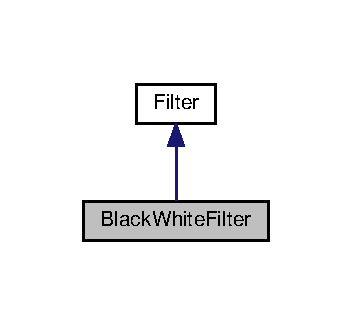
\includegraphics[width=169pt]{classModel_1_1BlackWhiteFilter__inherit__graph}
\end{center}
\end{figure}
\subsection*{Public Member Functions}
\begin{DoxyCompactItemize}
\item 
\hyperlink{classModel_1_1BlackWhiteFilter_a9a1028cd3e4eac0ac0891811507dfd2e}{Black\+White\+Filter} ()
\item 
string \hyperlink{classModel_1_1BlackWhiteFilter_a11335e13e50af74108bf926dc1340b4b}{get\+Name} ()
\item 
string \hyperlink{classModel_1_1BlackWhiteFilter_a62b7b60e24f92234393b840b35808e06}{get\+Filter\+Description} ()
\end{DoxyCompactItemize}
\subsection*{Additional Inherited Members}


\subsection{Detailed Description}
Converts the video to a black and white video. 

\subsection{Constructor \& Destructor Documentation}
\hypertarget{classModel_1_1BlackWhiteFilter_a9a1028cd3e4eac0ac0891811507dfd2e}{}\index{Model\+::\+Black\+White\+Filter@{Model\+::\+Black\+White\+Filter}!Black\+White\+Filter@{Black\+White\+Filter}}
\index{Black\+White\+Filter@{Black\+White\+Filter}!Model\+::\+Black\+White\+Filter@{Model\+::\+Black\+White\+Filter}}
\subsubsection[{Black\+White\+Filter}]{\setlength{\rightskip}{0pt plus 5cm}{\bf Black\+White\+Filter} (
\begin{DoxyParamCaption}
{}
\end{DoxyParamCaption}
)}\label{classModel_1_1BlackWhiteFilter_a9a1028cd3e4eac0ac0891811507dfd2e}


Constructor. 



\subsection{Member Function Documentation}
\hypertarget{classModel_1_1BlackWhiteFilter_a62b7b60e24f92234393b840b35808e06}{}\index{Model\+::\+Black\+White\+Filter@{Model\+::\+Black\+White\+Filter}!get\+Filter\+Description@{get\+Filter\+Description}}
\index{get\+Filter\+Description@{get\+Filter\+Description}!Model\+::\+Black\+White\+Filter@{Model\+::\+Black\+White\+Filter}}
\subsubsection[{get\+Filter\+Description}]{\setlength{\rightskip}{0pt plus 5cm}string get\+Filter\+Description (
\begin{DoxyParamCaption}
{}
\end{DoxyParamCaption}
)\hspace{0.3cm}{\ttfamily [virtual]}}\label{classModel_1_1BlackWhiteFilter_a62b7b60e24f92234393b840b35808e06}


Returns the string that the ffmpeg library needs to apply the filter to a video. 

\begin{DoxyReturn}{Returns}
The string for the ffmpeg library.
\end{DoxyReturn}


Implements \hyperlink{classModel_1_1Filter_a453fcafa809afa1ce58d9ef95d5f26c0}{Filter}.

\hypertarget{classModel_1_1BlackWhiteFilter_a11335e13e50af74108bf926dc1340b4b}{}\index{Model\+::\+Black\+White\+Filter@{Model\+::\+Black\+White\+Filter}!get\+Name@{get\+Name}}
\index{get\+Name@{get\+Name}!Model\+::\+Black\+White\+Filter@{Model\+::\+Black\+White\+Filter}}
\subsubsection[{get\+Name}]{\setlength{\rightskip}{0pt plus 5cm}string get\+Name (
\begin{DoxyParamCaption}
{}
\end{DoxyParamCaption}
)\hspace{0.3cm}{\ttfamily [virtual]}}\label{classModel_1_1BlackWhiteFilter_a11335e13e50af74108bf926dc1340b4b}


Returns the name of the filter. 

\begin{DoxyReturn}{Returns}
The filtername.
\end{DoxyReturn}


Implements \hyperlink{classModel_1_1Filter_ade93aa98c68d185a9c03784d36140225}{Filter}.


\newpage\hypertarget{classModel_1_1BlendingFilter}{}\section{Blending\+Filter Class Reference}
\label{classModel_1_1BlendingFilter}\index{Blending\+Filter@{Blending\+Filter}}


Inheritance diagram for Blending\+Filter\+:
\nopagebreak
\begin{figure}[H]
\begin{center}
\leavevmode
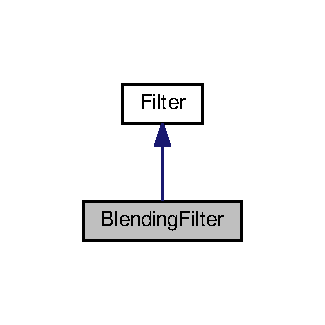
\includegraphics[width=156pt]{classModel_1_1BlendingFilter__inherit__graph}
\end{center}
\end{figure}
\subsection*{Public Member Functions}
\begin{DoxyCompactItemize}
\item 
\hyperlink{classModel_1_1BlendingFilter_aef4d8116cdf1f472bfc3f294a324a68d}{Blending\+Filter} ()
\item 
bool \hyperlink{classModel_1_1BlendingFilter_a323aa2fded0187976205e9bd41455108}{get\+In\+Blend} ()
\item 
void \hyperlink{classModel_1_1BlendingFilter_a4b3c5d143c333646fc19059b52d91f98}{set\+In\+Blend} (bool \hyperlink{classModel_1_1BlendingFilter_a5236a1acd21870beccb3622a0d868f64}{in\+Blend})
\item 
int \hyperlink{classModel_1_1BlendingFilter_ab75960aceca9106a2d1e4ac528e5c00f}{get\+Start\+Frame} ()
\item 
void \hyperlink{classModel_1_1BlendingFilter_aef2a28543fc8ddf9225491e032590c9c}{set\+Start\+Frame} (int \hyperlink{classModel_1_1BlendingFilter_a2c832c53905dc1fcfff946674d89f01d}{start\+Frame})
\item 
int \hyperlink{classModel_1_1BlendingFilter_a46a1b77243525a05a4c5594b00c7be28}{get\+End\+Frame} ()
\item 
void \hyperlink{classModel_1_1BlendingFilter_a87b980b1874e8518ddb597d74bd3c832}{set\+End\+Frame} (int \hyperlink{classModel_1_1BlendingFilter_ae86f112663a85130f9a8de28ca0070cb}{end\+Frame})
\item 
string \hyperlink{classModel_1_1BlendingFilter_a11335e13e50af74108bf926dc1340b4b}{get\+Name} ()
\item 
string \hyperlink{classModel_1_1BlendingFilter_a62b7b60e24f92234393b840b35808e06}{get\+Filter\+Description} ()
\end{DoxyCompactItemize}
\subsection*{Private Attributes}
\begin{DoxyCompactItemize}
\item 
bool \hyperlink{classModel_1_1BlendingFilter_a5236a1acd21870beccb3622a0d868f64}{in\+Blend}
\item 
int \hyperlink{classModel_1_1BlendingFilter_a2c832c53905dc1fcfff946674d89f01d}{start\+Frame}
\item 
int \hyperlink{classModel_1_1BlendingFilter_ae86f112663a85130f9a8de28ca0070cb}{end\+Frame}
\end{DoxyCompactItemize}
\subsection*{Additional Inherited Members}


\subsection{Detailed Description}
Inserts black blending into the video 

\subsection{Constructor \& Destructor Documentation}
\hypertarget{classModel_1_1BlendingFilter_aef4d8116cdf1f472bfc3f294a324a68d}{}\index{Model\+::\+Blending\+Filter@{Model\+::\+Blending\+Filter}!Blending\+Filter@{Blending\+Filter}}
\index{Blending\+Filter@{Blending\+Filter}!Model\+::\+Blending\+Filter@{Model\+::\+Blending\+Filter}}
\subsubsection[{Blending\+Filter}]{\setlength{\rightskip}{0pt plus 5cm}{\bf Blending\+Filter} (
\begin{DoxyParamCaption}
{}
\end{DoxyParamCaption}
)}\label{classModel_1_1BlendingFilter_aef4d8116cdf1f472bfc3f294a324a68d}


Constructor. 



\subsection{Member Function Documentation}
\hypertarget{classModel_1_1BlendingFilter_a46a1b77243525a05a4c5594b00c7be28}{}\index{Model\+::\+Blending\+Filter@{Model\+::\+Blending\+Filter}!get\+End\+Frame@{get\+End\+Frame}}
\index{get\+End\+Frame@{get\+End\+Frame}!Model\+::\+Blending\+Filter@{Model\+::\+Blending\+Filter}}
\subsubsection[{get\+End\+Frame}]{\setlength{\rightskip}{0pt plus 5cm}int get\+End\+Frame (
\begin{DoxyParamCaption}
{}
\end{DoxyParamCaption}
)}\label{classModel_1_1BlendingFilter_a46a1b77243525a05a4c5594b00c7be28}


Returns the end frame of the blending. 

\begin{DoxyReturn}{Returns}
The end frame.
\end{DoxyReturn}
\hypertarget{classModel_1_1BlendingFilter_a62b7b60e24f92234393b840b35808e06}{}\index{Model\+::\+Blending\+Filter@{Model\+::\+Blending\+Filter}!get\+Filter\+Description@{get\+Filter\+Description}}
\index{get\+Filter\+Description@{get\+Filter\+Description}!Model\+::\+Blending\+Filter@{Model\+::\+Blending\+Filter}}
\subsubsection[{get\+Filter\+Description}]{\setlength{\rightskip}{0pt plus 5cm}string get\+Filter\+Description (
\begin{DoxyParamCaption}
{}
\end{DoxyParamCaption}
)\hspace{0.3cm}{\ttfamily [virtual]}}\label{classModel_1_1BlendingFilter_a62b7b60e24f92234393b840b35808e06}


Returns the string that the ffmpeg library needs to apply the filter to a video. 

\begin{DoxyReturn}{Returns}
The string for the ffmpeg library.
\end{DoxyReturn}


Implements \hyperlink{classModel_1_1Filter_a453fcafa809afa1ce58d9ef95d5f26c0}{Filter}.

\hypertarget{classModel_1_1BlendingFilter_a323aa2fded0187976205e9bd41455108}{}\index{Model\+::\+Blending\+Filter@{Model\+::\+Blending\+Filter}!get\+In\+Blend@{get\+In\+Blend}}
\index{get\+In\+Blend@{get\+In\+Blend}!Model\+::\+Blending\+Filter@{Model\+::\+Blending\+Filter}}
\subsubsection[{get\+In\+Blend}]{\setlength{\rightskip}{0pt plus 5cm}bool get\+In\+Blend (
\begin{DoxyParamCaption}
{}
\end{DoxyParamCaption}
)}\label{classModel_1_1BlendingFilter_a323aa2fded0187976205e9bd41455108}


Whether it is an in blending. 

\begin{DoxyReturn}{Returns}
true if it is an in blending.
\end{DoxyReturn}
\hypertarget{classModel_1_1BlendingFilter_a11335e13e50af74108bf926dc1340b4b}{}\index{Model\+::\+Blending\+Filter@{Model\+::\+Blending\+Filter}!get\+Name@{get\+Name}}
\index{get\+Name@{get\+Name}!Model\+::\+Blending\+Filter@{Model\+::\+Blending\+Filter}}
\subsubsection[{get\+Name}]{\setlength{\rightskip}{0pt plus 5cm}string get\+Name (
\begin{DoxyParamCaption}
{}
\end{DoxyParamCaption}
)\hspace{0.3cm}{\ttfamily [virtual]}}\label{classModel_1_1BlendingFilter_a11335e13e50af74108bf926dc1340b4b}


Returns the name of the filter. 

\begin{DoxyReturn}{Returns}
The filtername.
\end{DoxyReturn}


Implements \hyperlink{classModel_1_1Filter_ade93aa98c68d185a9c03784d36140225}{Filter}.

\hypertarget{classModel_1_1BlendingFilter_ab75960aceca9106a2d1e4ac528e5c00f}{}\index{Model\+::\+Blending\+Filter@{Model\+::\+Blending\+Filter}!get\+Start\+Frame@{get\+Start\+Frame}}
\index{get\+Start\+Frame@{get\+Start\+Frame}!Model\+::\+Blending\+Filter@{Model\+::\+Blending\+Filter}}
\subsubsection[{get\+Start\+Frame}]{\setlength{\rightskip}{0pt plus 5cm}int get\+Start\+Frame (
\begin{DoxyParamCaption}
{}
\end{DoxyParamCaption}
)}\label{classModel_1_1BlendingFilter_ab75960aceca9106a2d1e4ac528e5c00f}


Returns the start frame of the blending. 

\begin{DoxyReturn}{Returns}
The start frame of the blending.
\end{DoxyReturn}
\hypertarget{classModel_1_1BlendingFilter_a87b980b1874e8518ddb597d74bd3c832}{}\index{Model\+::\+Blending\+Filter@{Model\+::\+Blending\+Filter}!set\+End\+Frame@{set\+End\+Frame}}
\index{set\+End\+Frame@{set\+End\+Frame}!Model\+::\+Blending\+Filter@{Model\+::\+Blending\+Filter}}
\subsubsection[{set\+End\+Frame}]{\setlength{\rightskip}{0pt plus 5cm}void set\+End\+Frame (
\begin{DoxyParamCaption}
\item[{int}]{end\+Frame}
\end{DoxyParamCaption}
)}\label{classModel_1_1BlendingFilter_a87b980b1874e8518ddb597d74bd3c832}


Sets the end frame of the blending. 


\begin{DoxyParams}{Parameters}
{\em end\+Frame} & The end frame.\\
\hline
\end{DoxyParams}
\hypertarget{classModel_1_1BlendingFilter_a4b3c5d143c333646fc19059b52d91f98}{}\index{Model\+::\+Blending\+Filter@{Model\+::\+Blending\+Filter}!set\+In\+Blend@{set\+In\+Blend}}
\index{set\+In\+Blend@{set\+In\+Blend}!Model\+::\+Blending\+Filter@{Model\+::\+Blending\+Filter}}
\subsubsection[{set\+In\+Blend}]{\setlength{\rightskip}{0pt plus 5cm}void set\+In\+Blend (
\begin{DoxyParamCaption}
\item[{bool}]{in\+Blend}
\end{DoxyParamCaption}
)}\label{classModel_1_1BlendingFilter_a4b3c5d143c333646fc19059b52d91f98}


Sets whether it is an in blending. 


\begin{DoxyParams}{Parameters}
{\em in\+Blend} & True if it is an in blending.\\
\hline
\end{DoxyParams}
\hypertarget{classModel_1_1BlendingFilter_aef2a28543fc8ddf9225491e032590c9c}{}\index{Model\+::\+Blending\+Filter@{Model\+::\+Blending\+Filter}!set\+Start\+Frame@{set\+Start\+Frame}}
\index{set\+Start\+Frame@{set\+Start\+Frame}!Model\+::\+Blending\+Filter@{Model\+::\+Blending\+Filter}}
\subsubsection[{set\+Start\+Frame}]{\setlength{\rightskip}{0pt plus 5cm}void set\+Start\+Frame (
\begin{DoxyParamCaption}
\item[{int}]{start\+Frame}
\end{DoxyParamCaption}
)}\label{classModel_1_1BlendingFilter_aef2a28543fc8ddf9225491e032590c9c}


Sets the start frame of the blending. 


\begin{DoxyParams}{Parameters}
{\em start\+Frame} & The start frame.\\
\hline
\end{DoxyParams}


\subsection{Field Documentation}
\hypertarget{classModel_1_1BlendingFilter_ae86f112663a85130f9a8de28ca0070cb}{}\index{Model\+::\+Blending\+Filter@{Model\+::\+Blending\+Filter}!end\+Frame@{end\+Frame}}
\index{end\+Frame@{end\+Frame}!Model\+::\+Blending\+Filter@{Model\+::\+Blending\+Filter}}
\subsubsection[{end\+Frame}]{\setlength{\rightskip}{0pt plus 5cm}int end\+Frame\hspace{0.3cm}{\ttfamily [private]}}\label{classModel_1_1BlendingFilter_ae86f112663a85130f9a8de28ca0070cb}
\hypertarget{classModel_1_1BlendingFilter_a5236a1acd21870beccb3622a0d868f64}{}\index{Model\+::\+Blending\+Filter@{Model\+::\+Blending\+Filter}!in\+Blend@{in\+Blend}}
\index{in\+Blend@{in\+Blend}!Model\+::\+Blending\+Filter@{Model\+::\+Blending\+Filter}}
\subsubsection[{in\+Blend}]{\setlength{\rightskip}{0pt plus 5cm}bool in\+Blend\hspace{0.3cm}{\ttfamily [private]}}\label{classModel_1_1BlendingFilter_a5236a1acd21870beccb3622a0d868f64}
\hypertarget{classModel_1_1BlendingFilter_a2c832c53905dc1fcfff946674d89f01d}{}\index{Model\+::\+Blending\+Filter@{Model\+::\+Blending\+Filter}!start\+Frame@{start\+Frame}}
\index{start\+Frame@{start\+Frame}!Model\+::\+Blending\+Filter@{Model\+::\+Blending\+Filter}}
\subsubsection[{start\+Frame}]{\setlength{\rightskip}{0pt plus 5cm}int start\+Frame\hspace{0.3cm}{\ttfamily [private]}}\label{classModel_1_1BlendingFilter_a2c832c53905dc1fcfff946674d89f01d}

\newpage\hypertarget{classGUI_1_1BlendingFilterBox}{}\section{Blending\+Filter\+Box Class Reference}
\label{classGUI_1_1BlendingFilterBox}\index{Blending\+Filter\+Box@{Blending\+Filter\+Box}}


Inheritance diagram for Blending\+Filter\+Box\+:
\nopagebreak
\begin{figure}[H]
\begin{center}
\leavevmode
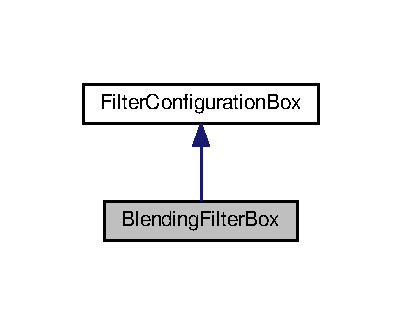
\includegraphics[width=193pt]{classGUI_1_1BlendingFilterBox__inherit__graph}
\end{center}
\end{figure}
\subsection*{Public Member Functions}
\begin{DoxyCompactItemize}
\item 
\hyperlink{classGUI_1_1BlendingFilterBox_a0aa76c7477d619b7738af743e0e5bb18}{Blending\+Filter\+Box} (\hyperlink{classGUI_1_1QWidget}{G\+U\+I\+::\+Q\+Widget} $\ast$parent)
\end{DoxyCompactItemize}
\subsection*{Additional Inherited Members}


\subsection{Detailed Description}
This class contains the gui elements for changing the options of a blending filter. 

\subsection{Constructor \& Destructor Documentation}
\hypertarget{classGUI_1_1BlendingFilterBox_a0aa76c7477d619b7738af743e0e5bb18}{}\index{G\+U\+I\+::\+Blending\+Filter\+Box@{G\+U\+I\+::\+Blending\+Filter\+Box}!Blending\+Filter\+Box@{Blending\+Filter\+Box}}
\index{Blending\+Filter\+Box@{Blending\+Filter\+Box}!G\+U\+I\+::\+Blending\+Filter\+Box@{G\+U\+I\+::\+Blending\+Filter\+Box}}
\subsubsection[{Blending\+Filter\+Box}]{\setlength{\rightskip}{0pt plus 5cm}{\bf Blending\+Filter\+Box} (
\begin{DoxyParamCaption}
\item[{{\bf G\+U\+I\+::\+Q\+Widget} $\ast$}]{parent}
\end{DoxyParamCaption}
)}\label{classGUI_1_1BlendingFilterBox_a0aa76c7477d619b7738af743e0e5bb18}


Constructor. 


\newpage\hypertarget{classModel_1_1BlurFilter}{}\section{Blur\+Filter Class Reference}
\label{classModel_1_1BlurFilter}\index{Blur\+Filter@{Blur\+Filter}}


Inheritance diagram for Blur\+Filter\+:
\nopagebreak
\begin{figure}[H]
\begin{center}
\leavevmode
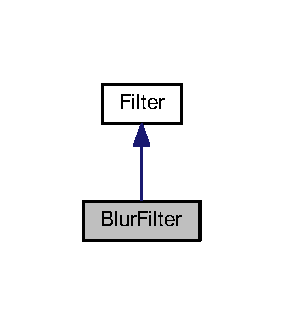
\includegraphics[width=136pt]{classModel_1_1BlurFilter__inherit__graph}
\end{center}
\end{figure}
\subsection*{Public Member Functions}
\begin{DoxyCompactItemize}
\item 
\hyperlink{classModel_1_1BlurFilter_afe4d07071313db8ac2e61b2641051b21}{Blur\+Filter} ()
\item 
bool \hyperlink{classModel_1_1BlurFilter_a0f68baff76107f2b3982df5cca754340}{get\+Preserve\+Edges} ()
\item 
void \hyperlink{classModel_1_1BlurFilter_a87c0326c6cec136fccffeca502d20ede}{set\+Preserve\+Edges} (bool \hyperlink{classModel_1_1BlurFilter_a063a2e7e7a9dbc091f483eeaec61d5e3}{preserve\+Edges})
\item 
int \hyperlink{classModel_1_1BlurFilter_a708995fb1b6acb31ee0dfb0f4881e5b5}{get\+Intensity} ()
\item 
void \hyperlink{classModel_1_1BlurFilter_ac8255ffbc46bb61acaa8fd23d0d260eb}{set\+Intensity} (int \hyperlink{classModel_1_1BlurFilter_a299ec0c42ccc5a2d79d1739428ac3210}{intensity})
\item 
string \hyperlink{classModel_1_1BlurFilter_a62b7b60e24f92234393b840b35808e06}{get\+Filter\+Description} ()
\item 
string \hyperlink{classModel_1_1BlurFilter_a11335e13e50af74108bf926dc1340b4b}{get\+Name} ()
\end{DoxyCompactItemize}
\subsection*{Private Attributes}
\begin{DoxyCompactItemize}
\item 
bool \hyperlink{classModel_1_1BlurFilter_a063a2e7e7a9dbc091f483eeaec61d5e3}{preserve\+Edges}
\item 
int \hyperlink{classModel_1_1BlurFilter_a299ec0c42ccc5a2d79d1739428ac3210}{intensity}
\end{DoxyCompactItemize}
\subsection*{Additional Inherited Members}


\subsection{Detailed Description}
Blurs the video. 

\subsection{Constructor \& Destructor Documentation}
\hypertarget{classModel_1_1BlurFilter_afe4d07071313db8ac2e61b2641051b21}{}\index{Model\+::\+Blur\+Filter@{Model\+::\+Blur\+Filter}!Blur\+Filter@{Blur\+Filter}}
\index{Blur\+Filter@{Blur\+Filter}!Model\+::\+Blur\+Filter@{Model\+::\+Blur\+Filter}}
\subsubsection[{Blur\+Filter}]{\setlength{\rightskip}{0pt plus 5cm}{\bf Blur\+Filter} (
\begin{DoxyParamCaption}
{}
\end{DoxyParamCaption}
)}\label{classModel_1_1BlurFilter_afe4d07071313db8ac2e61b2641051b21}


Constructor. 



\subsection{Member Function Documentation}
\hypertarget{classModel_1_1BlurFilter_a62b7b60e24f92234393b840b35808e06}{}\index{Model\+::\+Blur\+Filter@{Model\+::\+Blur\+Filter}!get\+Filter\+Description@{get\+Filter\+Description}}
\index{get\+Filter\+Description@{get\+Filter\+Description}!Model\+::\+Blur\+Filter@{Model\+::\+Blur\+Filter}}
\subsubsection[{get\+Filter\+Description}]{\setlength{\rightskip}{0pt plus 5cm}string get\+Filter\+Description (
\begin{DoxyParamCaption}
{}
\end{DoxyParamCaption}
)\hspace{0.3cm}{\ttfamily [virtual]}}\label{classModel_1_1BlurFilter_a62b7b60e24f92234393b840b35808e06}


Returns the string that the ffmpeg library needs to apply the filter to a video. 

\begin{DoxyReturn}{Returns}
The string for the ffmpeg library.
\end{DoxyReturn}


Implements \hyperlink{classModel_1_1Filter_a453fcafa809afa1ce58d9ef95d5f26c0}{Filter}.

\hypertarget{classModel_1_1BlurFilter_a708995fb1b6acb31ee0dfb0f4881e5b5}{}\index{Model\+::\+Blur\+Filter@{Model\+::\+Blur\+Filter}!get\+Intensity@{get\+Intensity}}
\index{get\+Intensity@{get\+Intensity}!Model\+::\+Blur\+Filter@{Model\+::\+Blur\+Filter}}
\subsubsection[{get\+Intensity}]{\setlength{\rightskip}{0pt plus 5cm}int get\+Intensity (
\begin{DoxyParamCaption}
{}
\end{DoxyParamCaption}
)}\label{classModel_1_1BlurFilter_a708995fb1b6acb31ee0dfb0f4881e5b5}


Returns the intensity of the blurring. 

\begin{DoxyReturn}{Returns}
The intensity of the blurring.
\end{DoxyReturn}
\hypertarget{classModel_1_1BlurFilter_a11335e13e50af74108bf926dc1340b4b}{}\index{Model\+::\+Blur\+Filter@{Model\+::\+Blur\+Filter}!get\+Name@{get\+Name}}
\index{get\+Name@{get\+Name}!Model\+::\+Blur\+Filter@{Model\+::\+Blur\+Filter}}
\subsubsection[{get\+Name}]{\setlength{\rightskip}{0pt plus 5cm}string get\+Name (
\begin{DoxyParamCaption}
{}
\end{DoxyParamCaption}
)\hspace{0.3cm}{\ttfamily [virtual]}}\label{classModel_1_1BlurFilter_a11335e13e50af74108bf926dc1340b4b}


Returns the name of the filter. 

\begin{DoxyReturn}{Returns}
The filtername.
\end{DoxyReturn}


Implements \hyperlink{classModel_1_1Filter_ade93aa98c68d185a9c03784d36140225}{Filter}.

\hypertarget{classModel_1_1BlurFilter_a0f68baff76107f2b3982df5cca754340}{}\index{Model\+::\+Blur\+Filter@{Model\+::\+Blur\+Filter}!get\+Preserve\+Edges@{get\+Preserve\+Edges}}
\index{get\+Preserve\+Edges@{get\+Preserve\+Edges}!Model\+::\+Blur\+Filter@{Model\+::\+Blur\+Filter}}
\subsubsection[{get\+Preserve\+Edges}]{\setlength{\rightskip}{0pt plus 5cm}bool get\+Preserve\+Edges (
\begin{DoxyParamCaption}
{}
\end{DoxyParamCaption}
)}\label{classModel_1_1BlurFilter_a0f68baff76107f2b3982df5cca754340}


Whether edges shall be preserved when blurring. 

\begin{DoxyReturn}{Returns}
true if the edges are preserved.
\end{DoxyReturn}
\hypertarget{classModel_1_1BlurFilter_ac8255ffbc46bb61acaa8fd23d0d260eb}{}\index{Model\+::\+Blur\+Filter@{Model\+::\+Blur\+Filter}!set\+Intensity@{set\+Intensity}}
\index{set\+Intensity@{set\+Intensity}!Model\+::\+Blur\+Filter@{Model\+::\+Blur\+Filter}}
\subsubsection[{set\+Intensity}]{\setlength{\rightskip}{0pt plus 5cm}void set\+Intensity (
\begin{DoxyParamCaption}
\item[{int}]{intensity}
\end{DoxyParamCaption}
)}\label{classModel_1_1BlurFilter_ac8255ffbc46bb61acaa8fd23d0d260eb}


Sets the intensity of the blurring. 


\begin{DoxyParams}{Parameters}
{\em intensity} & The intensity of the blurring.\\
\hline
\end{DoxyParams}
\hypertarget{classModel_1_1BlurFilter_a87c0326c6cec136fccffeca502d20ede}{}\index{Model\+::\+Blur\+Filter@{Model\+::\+Blur\+Filter}!set\+Preserve\+Edges@{set\+Preserve\+Edges}}
\index{set\+Preserve\+Edges@{set\+Preserve\+Edges}!Model\+::\+Blur\+Filter@{Model\+::\+Blur\+Filter}}
\subsubsection[{set\+Preserve\+Edges}]{\setlength{\rightskip}{0pt plus 5cm}void set\+Preserve\+Edges (
\begin{DoxyParamCaption}
\item[{bool}]{preserve\+Edges}
\end{DoxyParamCaption}
)}\label{classModel_1_1BlurFilter_a87c0326c6cec136fccffeca502d20ede}


Sets whether the edges shall be preserved when blurring. 


\begin{DoxyParams}{Parameters}
{\em preserve\+Edges} & True if the edges shall be preserved.\\
\hline
\end{DoxyParams}


\subsection{Field Documentation}
\hypertarget{classModel_1_1BlurFilter_a299ec0c42ccc5a2d79d1739428ac3210}{}\index{Model\+::\+Blur\+Filter@{Model\+::\+Blur\+Filter}!intensity@{intensity}}
\index{intensity@{intensity}!Model\+::\+Blur\+Filter@{Model\+::\+Blur\+Filter}}
\subsubsection[{intensity}]{\setlength{\rightskip}{0pt plus 5cm}int intensity\hspace{0.3cm}{\ttfamily [private]}}\label{classModel_1_1BlurFilter_a299ec0c42ccc5a2d79d1739428ac3210}
\hypertarget{classModel_1_1BlurFilter_a063a2e7e7a9dbc091f483eeaec61d5e3}{}\index{Model\+::\+Blur\+Filter@{Model\+::\+Blur\+Filter}!preserve\+Edges@{preserve\+Edges}}
\index{preserve\+Edges@{preserve\+Edges}!Model\+::\+Blur\+Filter@{Model\+::\+Blur\+Filter}}
\subsubsection[{preserve\+Edges}]{\setlength{\rightskip}{0pt plus 5cm}bool preserve\+Edges\hspace{0.3cm}{\ttfamily [private]}}\label{classModel_1_1BlurFilter_a063a2e7e7a9dbc091f483eeaec61d5e3}

\newpage\hypertarget{classGUI_1_1BlurFilterBox}{}\section{Blur\+Filter\+Box Class Reference}
\label{classGUI_1_1BlurFilterBox}\index{Blur\+Filter\+Box@{Blur\+Filter\+Box}}
\subsection*{Public Member Functions}
\begin{DoxyCompactItemize}
\item 
\hyperlink{classGUI_1_1BlurFilterBox_aa337b8816e06853cd7d6e64c3e4dd76b}{Blur\+Filter\+Box} (\hyperlink{classGUI_1_1Player_1_1QWidget}{G\+U\+I\+::\+Player\+::\+Q\+Widget} $\ast$parent)
\end{DoxyCompactItemize}
\subsection*{Additional Inherited Members}


\subsection{Detailed Description}
This class contains the gui elements for changing the options of a blurring filter. 

\subsection{Constructor \& Destructor Documentation}
\hypertarget{classGUI_1_1BlurFilterBox_aa337b8816e06853cd7d6e64c3e4dd76b}{}\index{G\+U\+I\+::\+Blur\+Filter\+Box@{G\+U\+I\+::\+Blur\+Filter\+Box}!Blur\+Filter\+Box@{Blur\+Filter\+Box}}
\index{Blur\+Filter\+Box@{Blur\+Filter\+Box}!G\+U\+I\+::\+Blur\+Filter\+Box@{G\+U\+I\+::\+Blur\+Filter\+Box}}
\subsubsection[{Blur\+Filter\+Box}]{\setlength{\rightskip}{0pt plus 5cm}{\bf Blur\+Filter\+Box} (
\begin{DoxyParamCaption}
\item[{{\bf G\+U\+I\+::\+Player\+::\+Q\+Widget} $\ast$}]{parent}
\end{DoxyParamCaption}
)}\label{classGUI_1_1BlurFilterBox_aa337b8816e06853cd7d6e64c3e4dd76b}


Constructor. 


\newpage\hypertarget{classModel_1_1BorderFilter}{}\section{Border\+Filter Class Reference}
\label{classModel_1_1BorderFilter}\index{Border\+Filter@{Border\+Filter}}


Inheritance diagram for Border\+Filter\+:
\nopagebreak
\begin{figure}[H]
\begin{center}
\leavevmode
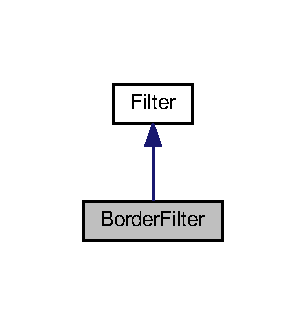
\includegraphics[width=147pt]{classModel_1_1BorderFilter__inherit__graph}
\end{center}
\end{figure}
\subsection*{Public Member Functions}
\begin{DoxyCompactItemize}
\item 
\hyperlink{classModel_1_1BorderFilter_a293d30704fa72a0dad9ea5ef7e473c38}{Border\+Filter} ()
\item 
bool \hyperlink{classModel_1_1BorderFilter_a7f662ce666098754b0916a828633f842}{get\+Top} ()
\item 
void \hyperlink{classModel_1_1BorderFilter_a41a3d0253d877ec681fc30f85ae21aed}{set\+Top} (bool \hyperlink{classModel_1_1BorderFilter_a5c6956f4ef8974f2548e3189232cf019}{top})
\item 
bool \hyperlink{classModel_1_1BorderFilter_ac96fcca335b0daaa5e216993666a7af2}{get\+Bottom} ()
\item 
void \hyperlink{classModel_1_1BorderFilter_ae60a4cf24fcd4cc34ca831917a609e79}{set\+Bottom} (bool \hyperlink{classModel_1_1BorderFilter_abb167350350ffbc934382b6d3ecafead}{bottom})
\item 
bool \hyperlink{classModel_1_1BorderFilter_a09836b29d544b94e145dd6a725887dd2}{get\+Right} ()
\item 
void \hyperlink{classModel_1_1BorderFilter_a18165f5951ddba8f3b25b2a199f90bc1}{set\+Right} (bool \hyperlink{classModel_1_1BorderFilter_acd047173db926d54ee91589f7ab53492}{right})
\item 
bool \hyperlink{classModel_1_1BorderFilter_afb561071d09e3b031b1d951c51e94f24}{get\+Left} ()
\item 
void \hyperlink{classModel_1_1BorderFilter_a07821fa96843dccb8ee4c9a711f1f43b}{set\+Left} (bool \hyperlink{classModel_1_1BorderFilter_aef0ceba738a4b7216ac568b5a5c137d3}{left})
\item 
int \hyperlink{classModel_1_1BorderFilter_ab6b7bfb33162f992d1bb4e8d6699abef}{get\+Thickness} ()
\item 
void \hyperlink{classModel_1_1BorderFilter_ae2faef96ee1277d229d6b6988c66e6d3}{set\+Thickness} (int \hyperlink{classModel_1_1BorderFilter_a4ae4bed5e7efe23b97dad176fe6524c3}{thickness})
\item 
Q\+Rgb \hyperlink{classModel_1_1BorderFilter_ae697defefbdf5f895406269b15758d91}{get\+Color} ()
\item 
void \hyperlink{classModel_1_1BorderFilter_ad858846447f303e473dc8004ef607666}{set\+Color} (Q\+Rgb \hyperlink{classModel_1_1BorderFilter_a6e0c08bd2043c82b2e837117d811db91}{color})
\item 
string \hyperlink{classModel_1_1BorderFilter_a11335e13e50af74108bf926dc1340b4b}{get\+Name} ()
\item 
string \hyperlink{classModel_1_1BorderFilter_a62b7b60e24f92234393b840b35808e06}{get\+Filter\+Description} ()
\end{DoxyCompactItemize}
\subsection*{Private Attributes}
\begin{DoxyCompactItemize}
\item 
bool \hyperlink{classModel_1_1BorderFilter_a5c6956f4ef8974f2548e3189232cf019}{top}
\item 
bool \hyperlink{classModel_1_1BorderFilter_abb167350350ffbc934382b6d3ecafead}{bottom}
\item 
bool \hyperlink{classModel_1_1BorderFilter_acd047173db926d54ee91589f7ab53492}{right}
\item 
bool \hyperlink{classModel_1_1BorderFilter_aef0ceba738a4b7216ac568b5a5c137d3}{left}
\item 
int \hyperlink{classModel_1_1BorderFilter_a4ae4bed5e7efe23b97dad176fe6524c3}{thickness}
\item 
Q\+Rgb \hyperlink{classModel_1_1BorderFilter_a6e0c08bd2043c82b2e837117d811db91}{color}
\end{DoxyCompactItemize}
\subsection*{Additional Inherited Members}


\subsection{Detailed Description}
Inserts border into the video 

\subsection{Constructor \& Destructor Documentation}
\hypertarget{classModel_1_1BorderFilter_a293d30704fa72a0dad9ea5ef7e473c38}{}\index{Model\+::\+Border\+Filter@{Model\+::\+Border\+Filter}!Border\+Filter@{Border\+Filter}}
\index{Border\+Filter@{Border\+Filter}!Model\+::\+Border\+Filter@{Model\+::\+Border\+Filter}}
\subsubsection[{Border\+Filter}]{\setlength{\rightskip}{0pt plus 5cm}{\bf Border\+Filter} (
\begin{DoxyParamCaption}
{}
\end{DoxyParamCaption}
)}\label{classModel_1_1BorderFilter_a293d30704fa72a0dad9ea5ef7e473c38}


Constructor. 



\subsection{Member Function Documentation}
\hypertarget{classModel_1_1BorderFilter_ac96fcca335b0daaa5e216993666a7af2}{}\index{Model\+::\+Border\+Filter@{Model\+::\+Border\+Filter}!get\+Bottom@{get\+Bottom}}
\index{get\+Bottom@{get\+Bottom}!Model\+::\+Border\+Filter@{Model\+::\+Border\+Filter}}
\subsubsection[{get\+Bottom}]{\setlength{\rightskip}{0pt plus 5cm}bool get\+Bottom (
\begin{DoxyParamCaption}
{}
\end{DoxyParamCaption}
)}\label{classModel_1_1BorderFilter_ac96fcca335b0daaa5e216993666a7af2}


Whether a border is inserted at the bottom. 

\begin{DoxyReturn}{Returns}
True if a border is inserted at the bottom.
\end{DoxyReturn}
\hypertarget{classModel_1_1BorderFilter_ae697defefbdf5f895406269b15758d91}{}\index{Model\+::\+Border\+Filter@{Model\+::\+Border\+Filter}!get\+Color@{get\+Color}}
\index{get\+Color@{get\+Color}!Model\+::\+Border\+Filter@{Model\+::\+Border\+Filter}}
\subsubsection[{get\+Color}]{\setlength{\rightskip}{0pt plus 5cm}Q\+Rgb get\+Color (
\begin{DoxyParamCaption}
{}
\end{DoxyParamCaption}
)}\label{classModel_1_1BorderFilter_ae697defefbdf5f895406269b15758d91}


Returns the color of the border, 

\begin{DoxyReturn}{Returns}
The border color.
\end{DoxyReturn}
\hypertarget{classModel_1_1BorderFilter_a62b7b60e24f92234393b840b35808e06}{}\index{Model\+::\+Border\+Filter@{Model\+::\+Border\+Filter}!get\+Filter\+Description@{get\+Filter\+Description}}
\index{get\+Filter\+Description@{get\+Filter\+Description}!Model\+::\+Border\+Filter@{Model\+::\+Border\+Filter}}
\subsubsection[{get\+Filter\+Description}]{\setlength{\rightskip}{0pt plus 5cm}string get\+Filter\+Description (
\begin{DoxyParamCaption}
{}
\end{DoxyParamCaption}
)\hspace{0.3cm}{\ttfamily [virtual]}}\label{classModel_1_1BorderFilter_a62b7b60e24f92234393b840b35808e06}


Returns the string that the ffmpeg library needs to apply the filter to a video. 

\begin{DoxyReturn}{Returns}
The string for the ffmpeg library.
\end{DoxyReturn}


Implements \hyperlink{classModel_1_1Filter_a453fcafa809afa1ce58d9ef95d5f26c0}{Filter}.

\hypertarget{classModel_1_1BorderFilter_afb561071d09e3b031b1d951c51e94f24}{}\index{Model\+::\+Border\+Filter@{Model\+::\+Border\+Filter}!get\+Left@{get\+Left}}
\index{get\+Left@{get\+Left}!Model\+::\+Border\+Filter@{Model\+::\+Border\+Filter}}
\subsubsection[{get\+Left}]{\setlength{\rightskip}{0pt plus 5cm}bool get\+Left (
\begin{DoxyParamCaption}
{}
\end{DoxyParamCaption}
)}\label{classModel_1_1BorderFilter_afb561071d09e3b031b1d951c51e94f24}


Whether a border is inserted at the left. 

\begin{DoxyReturn}{Returns}
True if a border is inserted at the left.
\end{DoxyReturn}
\hypertarget{classModel_1_1BorderFilter_a11335e13e50af74108bf926dc1340b4b}{}\index{Model\+::\+Border\+Filter@{Model\+::\+Border\+Filter}!get\+Name@{get\+Name}}
\index{get\+Name@{get\+Name}!Model\+::\+Border\+Filter@{Model\+::\+Border\+Filter}}
\subsubsection[{get\+Name}]{\setlength{\rightskip}{0pt plus 5cm}string get\+Name (
\begin{DoxyParamCaption}
{}
\end{DoxyParamCaption}
)\hspace{0.3cm}{\ttfamily [virtual]}}\label{classModel_1_1BorderFilter_a11335e13e50af74108bf926dc1340b4b}


Returns the name of the filter. 

\begin{DoxyReturn}{Returns}
The filtername.
\end{DoxyReturn}


Implements \hyperlink{classModel_1_1Filter_ade93aa98c68d185a9c03784d36140225}{Filter}.

\hypertarget{classModel_1_1BorderFilter_a09836b29d544b94e145dd6a725887dd2}{}\index{Model\+::\+Border\+Filter@{Model\+::\+Border\+Filter}!get\+Right@{get\+Right}}
\index{get\+Right@{get\+Right}!Model\+::\+Border\+Filter@{Model\+::\+Border\+Filter}}
\subsubsection[{get\+Right}]{\setlength{\rightskip}{0pt plus 5cm}bool get\+Right (
\begin{DoxyParamCaption}
{}
\end{DoxyParamCaption}
)}\label{classModel_1_1BorderFilter_a09836b29d544b94e145dd6a725887dd2}


Whether a border is inserted at the right. 

\begin{DoxyReturn}{Returns}
True if a border is inserted at the right.
\end{DoxyReturn}
\hypertarget{classModel_1_1BorderFilter_ab6b7bfb33162f992d1bb4e8d6699abef}{}\index{Model\+::\+Border\+Filter@{Model\+::\+Border\+Filter}!get\+Thickness@{get\+Thickness}}
\index{get\+Thickness@{get\+Thickness}!Model\+::\+Border\+Filter@{Model\+::\+Border\+Filter}}
\subsubsection[{get\+Thickness}]{\setlength{\rightskip}{0pt plus 5cm}int get\+Thickness (
\begin{DoxyParamCaption}
{}
\end{DoxyParamCaption}
)}\label{classModel_1_1BorderFilter_ab6b7bfb33162f992d1bb4e8d6699abef}


Returns the thickness of the border. 

\begin{DoxyReturn}{Returns}
The thickness of the border.
\end{DoxyReturn}
\hypertarget{classModel_1_1BorderFilter_a7f662ce666098754b0916a828633f842}{}\index{Model\+::\+Border\+Filter@{Model\+::\+Border\+Filter}!get\+Top@{get\+Top}}
\index{get\+Top@{get\+Top}!Model\+::\+Border\+Filter@{Model\+::\+Border\+Filter}}
\subsubsection[{get\+Top}]{\setlength{\rightskip}{0pt plus 5cm}bool get\+Top (
\begin{DoxyParamCaption}
{}
\end{DoxyParamCaption}
)}\label{classModel_1_1BorderFilter_a7f662ce666098754b0916a828633f842}


Whether a border is inserted at the top. 

\begin{DoxyReturn}{Returns}
True if a border is inserted at the top.
\end{DoxyReturn}
\hypertarget{classModel_1_1BorderFilter_ae60a4cf24fcd4cc34ca831917a609e79}{}\index{Model\+::\+Border\+Filter@{Model\+::\+Border\+Filter}!set\+Bottom@{set\+Bottom}}
\index{set\+Bottom@{set\+Bottom}!Model\+::\+Border\+Filter@{Model\+::\+Border\+Filter}}
\subsubsection[{set\+Bottom}]{\setlength{\rightskip}{0pt plus 5cm}void set\+Bottom (
\begin{DoxyParamCaption}
\item[{bool}]{bottom}
\end{DoxyParamCaption}
)}\label{classModel_1_1BorderFilter_ae60a4cf24fcd4cc34ca831917a609e79}


Sets whether a border is inserted at the bottom. 


\begin{DoxyParams}{Parameters}
{\em bottom} & True if a border is inserted at the bottom.\\
\hline
\end{DoxyParams}
\hypertarget{classModel_1_1BorderFilter_ad858846447f303e473dc8004ef607666}{}\index{Model\+::\+Border\+Filter@{Model\+::\+Border\+Filter}!set\+Color@{set\+Color}}
\index{set\+Color@{set\+Color}!Model\+::\+Border\+Filter@{Model\+::\+Border\+Filter}}
\subsubsection[{set\+Color}]{\setlength{\rightskip}{0pt plus 5cm}void set\+Color (
\begin{DoxyParamCaption}
\item[{Q\+Rgb}]{color}
\end{DoxyParamCaption}
)}\label{classModel_1_1BorderFilter_ad858846447f303e473dc8004ef607666}


Sets the color of the border, 


\begin{DoxyParams}{Parameters}
{\em color} & The new border color.\\
\hline
\end{DoxyParams}
\hypertarget{classModel_1_1BorderFilter_a07821fa96843dccb8ee4c9a711f1f43b}{}\index{Model\+::\+Border\+Filter@{Model\+::\+Border\+Filter}!set\+Left@{set\+Left}}
\index{set\+Left@{set\+Left}!Model\+::\+Border\+Filter@{Model\+::\+Border\+Filter}}
\subsubsection[{set\+Left}]{\setlength{\rightskip}{0pt plus 5cm}void set\+Left (
\begin{DoxyParamCaption}
\item[{bool}]{left}
\end{DoxyParamCaption}
)}\label{classModel_1_1BorderFilter_a07821fa96843dccb8ee4c9a711f1f43b}


Sets whether a border is inserted at the left. 


\begin{DoxyParams}{Parameters}
{\em left} & True if a border is inserted at the left.\\
\hline
\end{DoxyParams}
\hypertarget{classModel_1_1BorderFilter_a18165f5951ddba8f3b25b2a199f90bc1}{}\index{Model\+::\+Border\+Filter@{Model\+::\+Border\+Filter}!set\+Right@{set\+Right}}
\index{set\+Right@{set\+Right}!Model\+::\+Border\+Filter@{Model\+::\+Border\+Filter}}
\subsubsection[{set\+Right}]{\setlength{\rightskip}{0pt plus 5cm}void set\+Right (
\begin{DoxyParamCaption}
\item[{bool}]{right}
\end{DoxyParamCaption}
)}\label{classModel_1_1BorderFilter_a18165f5951ddba8f3b25b2a199f90bc1}


Sets whether a border is inserted at the right. 


\begin{DoxyParams}{Parameters}
{\em right} & True if a border is inserted at the right.\\
\hline
\end{DoxyParams}
\hypertarget{classModel_1_1BorderFilter_ae2faef96ee1277d229d6b6988c66e6d3}{}\index{Model\+::\+Border\+Filter@{Model\+::\+Border\+Filter}!set\+Thickness@{set\+Thickness}}
\index{set\+Thickness@{set\+Thickness}!Model\+::\+Border\+Filter@{Model\+::\+Border\+Filter}}
\subsubsection[{set\+Thickness}]{\setlength{\rightskip}{0pt plus 5cm}void set\+Thickness (
\begin{DoxyParamCaption}
\item[{int}]{thickness}
\end{DoxyParamCaption}
)}\label{classModel_1_1BorderFilter_ae2faef96ee1277d229d6b6988c66e6d3}


Sets the thickness of the border. 


\begin{DoxyParams}{Parameters}
{\em thickness} & The thickness.\\
\hline
\end{DoxyParams}
\hypertarget{classModel_1_1BorderFilter_a41a3d0253d877ec681fc30f85ae21aed}{}\index{Model\+::\+Border\+Filter@{Model\+::\+Border\+Filter}!set\+Top@{set\+Top}}
\index{set\+Top@{set\+Top}!Model\+::\+Border\+Filter@{Model\+::\+Border\+Filter}}
\subsubsection[{set\+Top}]{\setlength{\rightskip}{0pt plus 5cm}void set\+Top (
\begin{DoxyParamCaption}
\item[{bool}]{top}
\end{DoxyParamCaption}
)}\label{classModel_1_1BorderFilter_a41a3d0253d877ec681fc30f85ae21aed}


Sets whether a border is inserted at the top. 


\begin{DoxyParams}{Parameters}
{\em top} & True if a border is inserted at the top.\\
\hline
\end{DoxyParams}


\subsection{Field Documentation}
\hypertarget{classModel_1_1BorderFilter_abb167350350ffbc934382b6d3ecafead}{}\index{Model\+::\+Border\+Filter@{Model\+::\+Border\+Filter}!bottom@{bottom}}
\index{bottom@{bottom}!Model\+::\+Border\+Filter@{Model\+::\+Border\+Filter}}
\subsubsection[{bottom}]{\setlength{\rightskip}{0pt plus 5cm}bool bottom\hspace{0.3cm}{\ttfamily [private]}}\label{classModel_1_1BorderFilter_abb167350350ffbc934382b6d3ecafead}
\hypertarget{classModel_1_1BorderFilter_a6e0c08bd2043c82b2e837117d811db91}{}\index{Model\+::\+Border\+Filter@{Model\+::\+Border\+Filter}!color@{color}}
\index{color@{color}!Model\+::\+Border\+Filter@{Model\+::\+Border\+Filter}}
\subsubsection[{color}]{\setlength{\rightskip}{0pt plus 5cm}Q\+Rgb color\hspace{0.3cm}{\ttfamily [private]}}\label{classModel_1_1BorderFilter_a6e0c08bd2043c82b2e837117d811db91}
\hypertarget{classModel_1_1BorderFilter_aef0ceba738a4b7216ac568b5a5c137d3}{}\index{Model\+::\+Border\+Filter@{Model\+::\+Border\+Filter}!left@{left}}
\index{left@{left}!Model\+::\+Border\+Filter@{Model\+::\+Border\+Filter}}
\subsubsection[{left}]{\setlength{\rightskip}{0pt plus 5cm}bool left\hspace{0.3cm}{\ttfamily [private]}}\label{classModel_1_1BorderFilter_aef0ceba738a4b7216ac568b5a5c137d3}
\hypertarget{classModel_1_1BorderFilter_acd047173db926d54ee91589f7ab53492}{}\index{Model\+::\+Border\+Filter@{Model\+::\+Border\+Filter}!right@{right}}
\index{right@{right}!Model\+::\+Border\+Filter@{Model\+::\+Border\+Filter}}
\subsubsection[{right}]{\setlength{\rightskip}{0pt plus 5cm}bool right\hspace{0.3cm}{\ttfamily [private]}}\label{classModel_1_1BorderFilter_acd047173db926d54ee91589f7ab53492}
\hypertarget{classModel_1_1BorderFilter_a4ae4bed5e7efe23b97dad176fe6524c3}{}\index{Model\+::\+Border\+Filter@{Model\+::\+Border\+Filter}!thickness@{thickness}}
\index{thickness@{thickness}!Model\+::\+Border\+Filter@{Model\+::\+Border\+Filter}}
\subsubsection[{thickness}]{\setlength{\rightskip}{0pt plus 5cm}int thickness\hspace{0.3cm}{\ttfamily [private]}}\label{classModel_1_1BorderFilter_a4ae4bed5e7efe23b97dad176fe6524c3}
\hypertarget{classModel_1_1BorderFilter_a5c6956f4ef8974f2548e3189232cf019}{}\index{Model\+::\+Border\+Filter@{Model\+::\+Border\+Filter}!top@{top}}
\index{top@{top}!Model\+::\+Border\+Filter@{Model\+::\+Border\+Filter}}
\subsubsection[{top}]{\setlength{\rightskip}{0pt plus 5cm}bool top\hspace{0.3cm}{\ttfamily [private]}}\label{classModel_1_1BorderFilter_a5c6956f4ef8974f2548e3189232cf019}

\newpage\hypertarget{classGUI_1_1BorderFilterBox}{}\section{Border\+Filter\+Box Class Reference}
\label{classGUI_1_1BorderFilterBox}\index{Border\+Filter\+Box@{Border\+Filter\+Box}}


Inheritance diagram for Border\+Filter\+Box\+:
\nopagebreak
\begin{figure}[H]
\begin{center}
\leavevmode
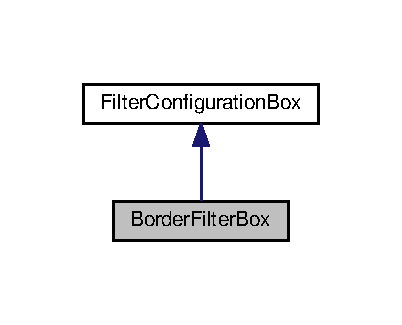
\includegraphics[width=193pt]{classGUI_1_1BorderFilterBox__inherit__graph}
\end{center}
\end{figure}
\subsection*{Public Member Functions}
\begin{DoxyCompactItemize}
\item 
\hyperlink{classGUI_1_1BorderFilterBox_a4b514b5fda573768947c8a82d79fa7b7}{Border\+Filter\+Box} (\hyperlink{classGUI_1_1QWidget}{G\+U\+I\+::\+Q\+Widget} $\ast$parent)
\end{DoxyCompactItemize}
\subsection*{Additional Inherited Members}


\subsection{Detailed Description}
This class contains the gui elements for changing the options of a border filter. 

\subsection{Constructor \& Destructor Documentation}
\hypertarget{classGUI_1_1BorderFilterBox_a4b514b5fda573768947c8a82d79fa7b7}{}\index{G\+U\+I\+::\+Border\+Filter\+Box@{G\+U\+I\+::\+Border\+Filter\+Box}!Border\+Filter\+Box@{Border\+Filter\+Box}}
\index{Border\+Filter\+Box@{Border\+Filter\+Box}!G\+U\+I\+::\+Border\+Filter\+Box@{G\+U\+I\+::\+Border\+Filter\+Box}}
\subsubsection[{Border\+Filter\+Box}]{\setlength{\rightskip}{0pt plus 5cm}{\bf Border\+Filter\+Box} (
\begin{DoxyParamCaption}
\item[{{\bf G\+U\+I\+::\+Q\+Widget} $\ast$}]{parent}
\end{DoxyParamCaption}
)}\label{classGUI_1_1BorderFilterBox_a4b514b5fda573768947c8a82d79fa7b7}


Constructor. 


\newpage\hypertarget{classModel_1_1BrightnessFilter}{}\section{Brightness\+Filter Class Reference}
\label{classModel_1_1BrightnessFilter}\index{Brightness\+Filter@{Brightness\+Filter}}


Inheritance diagram for Brightness\+Filter\+:
\nopagebreak
\begin{figure}[H]
\begin{center}
\leavevmode
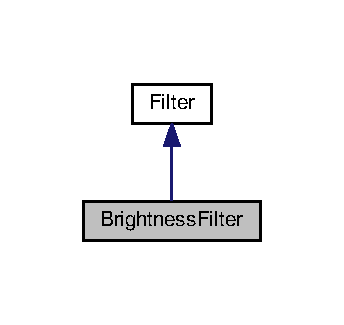
\includegraphics[width=165pt]{classModel_1_1BrightnessFilter__inherit__graph}
\end{center}
\end{figure}
\subsection*{Public Member Functions}
\begin{DoxyCompactItemize}
\item 
\hyperlink{classModel_1_1BrightnessFilter_a7be0e74d76ab6670dc2648d6833b9021}{Brightness\+Filter} ()
\item 
int \hyperlink{classModel_1_1BrightnessFilter_a708995fb1b6acb31ee0dfb0f4881e5b5}{get\+Intensity} ()
\item 
void \hyperlink{classModel_1_1BrightnessFilter_ac8255ffbc46bb61acaa8fd23d0d260eb}{set\+Intensity} (int \hyperlink{classModel_1_1BrightnessFilter_a299ec0c42ccc5a2d79d1739428ac3210}{intensity})
\item 
string \hyperlink{classModel_1_1BrightnessFilter_a11335e13e50af74108bf926dc1340b4b}{get\+Name} ()
\item 
string \hyperlink{classModel_1_1BrightnessFilter_a62b7b60e24f92234393b840b35808e06}{get\+Filter\+Description} ()
\end{DoxyCompactItemize}
\subsection*{Private Attributes}
\begin{DoxyCompactItemize}
\item 
int \hyperlink{classModel_1_1BrightnessFilter_a299ec0c42ccc5a2d79d1739428ac3210}{intensity}
\end{DoxyCompactItemize}
\subsection*{Additional Inherited Members}


\subsection{Detailed Description}
Adjusts the video brightness. 

\subsection{Constructor \& Destructor Documentation}
\hypertarget{classModel_1_1BrightnessFilter_a7be0e74d76ab6670dc2648d6833b9021}{}\index{Model\+::\+Brightness\+Filter@{Model\+::\+Brightness\+Filter}!Brightness\+Filter@{Brightness\+Filter}}
\index{Brightness\+Filter@{Brightness\+Filter}!Model\+::\+Brightness\+Filter@{Model\+::\+Brightness\+Filter}}
\subsubsection[{Brightness\+Filter}]{\setlength{\rightskip}{0pt plus 5cm}{\bf Brightness\+Filter} (
\begin{DoxyParamCaption}
{}
\end{DoxyParamCaption}
)}\label{classModel_1_1BrightnessFilter_a7be0e74d76ab6670dc2648d6833b9021}


Constructor. 



\subsection{Member Function Documentation}
\hypertarget{classModel_1_1BrightnessFilter_a62b7b60e24f92234393b840b35808e06}{}\index{Model\+::\+Brightness\+Filter@{Model\+::\+Brightness\+Filter}!get\+Filter\+Description@{get\+Filter\+Description}}
\index{get\+Filter\+Description@{get\+Filter\+Description}!Model\+::\+Brightness\+Filter@{Model\+::\+Brightness\+Filter}}
\subsubsection[{get\+Filter\+Description}]{\setlength{\rightskip}{0pt plus 5cm}string get\+Filter\+Description (
\begin{DoxyParamCaption}
{}
\end{DoxyParamCaption}
)\hspace{0.3cm}{\ttfamily [virtual]}}\label{classModel_1_1BrightnessFilter_a62b7b60e24f92234393b840b35808e06}


Returns the string that the ffmpeg library needs to apply the filter to a video. 

\begin{DoxyReturn}{Returns}
The string for the ffmpeg library.
\end{DoxyReturn}


Implements \hyperlink{classModel_1_1Filter_a453fcafa809afa1ce58d9ef95d5f26c0}{Filter}.

\hypertarget{classModel_1_1BrightnessFilter_a708995fb1b6acb31ee0dfb0f4881e5b5}{}\index{Model\+::\+Brightness\+Filter@{Model\+::\+Brightness\+Filter}!get\+Intensity@{get\+Intensity}}
\index{get\+Intensity@{get\+Intensity}!Model\+::\+Brightness\+Filter@{Model\+::\+Brightness\+Filter}}
\subsubsection[{get\+Intensity}]{\setlength{\rightskip}{0pt plus 5cm}int get\+Intensity (
\begin{DoxyParamCaption}
{}
\end{DoxyParamCaption}
)}\label{classModel_1_1BrightnessFilter_a708995fb1b6acb31ee0dfb0f4881e5b5}


Returns the intensity of the brightness. 

\begin{DoxyReturn}{Returns}
The intensity.
\end{DoxyReturn}
\hypertarget{classModel_1_1BrightnessFilter_a11335e13e50af74108bf926dc1340b4b}{}\index{Model\+::\+Brightness\+Filter@{Model\+::\+Brightness\+Filter}!get\+Name@{get\+Name}}
\index{get\+Name@{get\+Name}!Model\+::\+Brightness\+Filter@{Model\+::\+Brightness\+Filter}}
\subsubsection[{get\+Name}]{\setlength{\rightskip}{0pt plus 5cm}string get\+Name (
\begin{DoxyParamCaption}
{}
\end{DoxyParamCaption}
)\hspace{0.3cm}{\ttfamily [virtual]}}\label{classModel_1_1BrightnessFilter_a11335e13e50af74108bf926dc1340b4b}


Returns the name of the filter. 

\begin{DoxyReturn}{Returns}
The filtername.
\end{DoxyReturn}


Implements \hyperlink{classModel_1_1Filter_ade93aa98c68d185a9c03784d36140225}{Filter}.

\hypertarget{classModel_1_1BrightnessFilter_ac8255ffbc46bb61acaa8fd23d0d260eb}{}\index{Model\+::\+Brightness\+Filter@{Model\+::\+Brightness\+Filter}!set\+Intensity@{set\+Intensity}}
\index{set\+Intensity@{set\+Intensity}!Model\+::\+Brightness\+Filter@{Model\+::\+Brightness\+Filter}}
\subsubsection[{set\+Intensity}]{\setlength{\rightskip}{0pt plus 5cm}void set\+Intensity (
\begin{DoxyParamCaption}
\item[{int}]{intensity}
\end{DoxyParamCaption}
)}\label{classModel_1_1BrightnessFilter_ac8255ffbc46bb61acaa8fd23d0d260eb}


Sets the intensity of the brightness. 


\begin{DoxyParams}{Parameters}
{\em intensity} & The new intensity.\\
\hline
\end{DoxyParams}


\subsection{Field Documentation}
\hypertarget{classModel_1_1BrightnessFilter_a299ec0c42ccc5a2d79d1739428ac3210}{}\index{Model\+::\+Brightness\+Filter@{Model\+::\+Brightness\+Filter}!intensity@{intensity}}
\index{intensity@{intensity}!Model\+::\+Brightness\+Filter@{Model\+::\+Brightness\+Filter}}
\subsubsection[{intensity}]{\setlength{\rightskip}{0pt plus 5cm}int intensity\hspace{0.3cm}{\ttfamily [private]}}\label{classModel_1_1BrightnessFilter_a299ec0c42ccc5a2d79d1739428ac3210}

\newpage\hypertarget{classGUI_1_1BrightnessFilterBox}{}\section{Brightness\+Filter\+Box Class Reference}
\label{classGUI_1_1BrightnessFilterBox}\index{Brightness\+Filter\+Box@{Brightness\+Filter\+Box}}
\subsection*{Public Member Functions}
\begin{DoxyCompactItemize}
\item 
\hypertarget{classGUI_1_1BrightnessFilterBox_a37ebb44fb61750578debb2a51d2c00ce}{}{\bfseries Brightness\+Filter\+Box} (\hyperlink{classGUI_1_1QtGui_1_1QWidget____10}{G\+U\+I\+::\+Qt\+Gui\+::\+Q\+Widget\+\_\+\+\_\+10} $\ast$parent)\label{classGUI_1_1BrightnessFilterBox_a37ebb44fb61750578debb2a51d2c00ce}

\item 
\hypertarget{classGUI_1_1BrightnessFilterBox_ad7c0ee00fe3faac7942d75eec2a5342b}{}virtual void {\bfseries set\+Filter} (\hyperlink{classModel_1_1Filter_1_1Filter}{Model\+::\+Filter\+::\+Filter} \&filter)\label{classGUI_1_1BrightnessFilterBox_ad7c0ee00fe3faac7942d75eec2a5342b}

\item 
\hypertarget{classGUI_1_1BrightnessFilterBox_acef2029a93f4ab3a538cdb643b9c2613}{}virtual \hyperlink{classModel_1_1Filter_1_1Filter}{Model\+::\+Filter\+::\+Filter} $\ast$ {\bfseries get\+Filter} ()\label{classGUI_1_1BrightnessFilterBox_acef2029a93f4ab3a538cdb643b9c2613}

\end{DoxyCompactItemize}

\newpage\hypertarget{classModel_1_1ColorbalanceFilter}{}\section{Colorbalance\+Filter Class Reference}
\label{classModel_1_1ColorbalanceFilter}\index{Colorbalance\+Filter@{Colorbalance\+Filter}}


Inheritance diagram for Colorbalance\+Filter\+:
\nopagebreak
\begin{figure}[H]
\begin{center}
\leavevmode
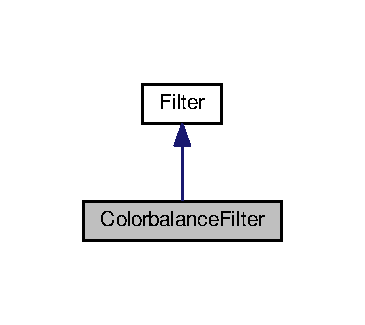
\includegraphics[width=175pt]{classModel_1_1ColorbalanceFilter__inherit__graph}
\end{center}
\end{figure}
\subsection*{Public Member Functions}
\begin{DoxyCompactItemize}
\item 
\hyperlink{classModel_1_1ColorbalanceFilter_a3ce5da414de521fd6406561b4b0c008b}{Colorbalance\+Filter} ()
\item 
\hyperlink{namespaceModel_a54742b2fc8f6a246926cbb87b7fae1a4}{Model\+::\+Basic\+Color} \hyperlink{classModel_1_1ColorbalanceFilter_a82ac188d01a7ce771cdb254e9eb70ba6}{get\+Color} ()
\item 
void \hyperlink{classModel_1_1ColorbalanceFilter_a707221b518c3ae5bf8ce16cc9b0d0054}{set\+Color} (\hyperlink{namespaceModel_a54742b2fc8f6a246926cbb87b7fae1a4}{Model\+::\+Basic\+Color} \hyperlink{classModel_1_1ColorbalanceFilter_af9c4a828f1030ef2b7d7ab814dd37cb9}{color})
\item 
int \hyperlink{classModel_1_1ColorbalanceFilter_a708995fb1b6acb31ee0dfb0f4881e5b5}{get\+Intensity} ()
\item 
void \hyperlink{classModel_1_1ColorbalanceFilter_ac8255ffbc46bb61acaa8fd23d0d260eb}{set\+Intensity} (int \hyperlink{classModel_1_1ColorbalanceFilter_a299ec0c42ccc5a2d79d1739428ac3210}{intensity})
\item 
bool \hyperlink{classModel_1_1ColorbalanceFilter_a1be0d343ed58d5d5bf7b816da375f190}{get\+Bright\+Pixels} ()
\item 
void \hyperlink{classModel_1_1ColorbalanceFilter_af0f286aa4c54fb1fd5813d02799da1cb}{set\+Bright\+Pixels} (bool \hyperlink{classModel_1_1ColorbalanceFilter_aae8fdd57ebeb891ebec4430ef4f71748}{bright\+Pixels})
\item 
bool \hyperlink{classModel_1_1ColorbalanceFilter_a71d3e0e416aa251b66678a14b4bfa1a1}{get\+Medium\+Pixels} ()
\item 
void \hyperlink{classModel_1_1ColorbalanceFilter_ab52d8f4be21efb3dbc9ef49adf755ace}{set\+Medium\+Pixels} (bool \hyperlink{classModel_1_1ColorbalanceFilter_a5d9db79c230cb372011e99b7a1799bc5}{medium\+Pixels})
\item 
string \hyperlink{classModel_1_1ColorbalanceFilter_a62b7b60e24f92234393b840b35808e06}{get\+Filter\+Description} ()
\item 
string \hyperlink{classModel_1_1ColorbalanceFilter_a11335e13e50af74108bf926dc1340b4b}{get\+Name} ()
\item 
bool \hyperlink{classModel_1_1ColorbalanceFilter_a81c4e5653e8217b741b4b183fe78abca}{get\+Dark\+Pixels} ()
\item 
void \hyperlink{classModel_1_1ColorbalanceFilter_a0215d6818f471e2d3ba48b52c2c3da5d}{set\+Dark\+Pixels} (bool \hyperlink{classModel_1_1ColorbalanceFilter_ab419b3e6552ab875fd167020998e8d45}{dark\+Pixels})
\end{DoxyCompactItemize}
\subsection*{Private Attributes}
\begin{DoxyCompactItemize}
\item 
int \hyperlink{classModel_1_1ColorbalanceFilter_a299ec0c42ccc5a2d79d1739428ac3210}{intensity}
\item 
bool \hyperlink{classModel_1_1ColorbalanceFilter_aae8fdd57ebeb891ebec4430ef4f71748}{bright\+Pixels}
\item 
bool \hyperlink{classModel_1_1ColorbalanceFilter_a5d9db79c230cb372011e99b7a1799bc5}{medium\+Pixels}
\item 
bool \hyperlink{classModel_1_1ColorbalanceFilter_ab419b3e6552ab875fd167020998e8d45}{dark\+Pixels}
\item 
\hyperlink{namespaceModel_a54742b2fc8f6a246926cbb87b7fae1a4}{Model\+::\+Basic\+Color} $\ast$ \hyperlink{classModel_1_1ColorbalanceFilter_af9c4a828f1030ef2b7d7ab814dd37cb9}{color}
\end{DoxyCompactItemize}
\subsection*{Additional Inherited Members}


\subsection{Detailed Description}
Adjusts the colorbalance of the video for the 3 basic colors. 

\subsection{Constructor \& Destructor Documentation}
\hypertarget{classModel_1_1ColorbalanceFilter_a3ce5da414de521fd6406561b4b0c008b}{}\index{Model\+::\+Colorbalance\+Filter@{Model\+::\+Colorbalance\+Filter}!Colorbalance\+Filter@{Colorbalance\+Filter}}
\index{Colorbalance\+Filter@{Colorbalance\+Filter}!Model\+::\+Colorbalance\+Filter@{Model\+::\+Colorbalance\+Filter}}
\subsubsection[{Colorbalance\+Filter}]{\setlength{\rightskip}{0pt plus 5cm}{\bf Colorbalance\+Filter} (
\begin{DoxyParamCaption}
{}
\end{DoxyParamCaption}
)}\label{classModel_1_1ColorbalanceFilter_a3ce5da414de521fd6406561b4b0c008b}


Constructor. 



\subsection{Member Function Documentation}
\hypertarget{classModel_1_1ColorbalanceFilter_a1be0d343ed58d5d5bf7b816da375f190}{}\index{Model\+::\+Colorbalance\+Filter@{Model\+::\+Colorbalance\+Filter}!get\+Bright\+Pixels@{get\+Bright\+Pixels}}
\index{get\+Bright\+Pixels@{get\+Bright\+Pixels}!Model\+::\+Colorbalance\+Filter@{Model\+::\+Colorbalance\+Filter}}
\subsubsection[{get\+Bright\+Pixels}]{\setlength{\rightskip}{0pt plus 5cm}bool get\+Bright\+Pixels (
\begin{DoxyParamCaption}
{}
\end{DoxyParamCaption}
)}\label{classModel_1_1ColorbalanceFilter_a1be0d343ed58d5d5bf7b816da375f190}


Whether the bright pixels shall be changed. 

\begin{DoxyReturn}{Returns}
True if the bright pixels are changed.
\end{DoxyReturn}
\hypertarget{classModel_1_1ColorbalanceFilter_a82ac188d01a7ce771cdb254e9eb70ba6}{}\index{Model\+::\+Colorbalance\+Filter@{Model\+::\+Colorbalance\+Filter}!get\+Color@{get\+Color}}
\index{get\+Color@{get\+Color}!Model\+::\+Colorbalance\+Filter@{Model\+::\+Colorbalance\+Filter}}
\subsubsection[{get\+Color}]{\setlength{\rightskip}{0pt plus 5cm}{\bf Model\+::\+Basic\+Color} get\+Color (
\begin{DoxyParamCaption}
{}
\end{DoxyParamCaption}
)}\label{classModel_1_1ColorbalanceFilter_a82ac188d01a7ce771cdb254e9eb70ba6}


Returns the color whose balance is to be changed. 

\begin{DoxyReturn}{Returns}
The color to change.
\end{DoxyReturn}
\hypertarget{classModel_1_1ColorbalanceFilter_a81c4e5653e8217b741b4b183fe78abca}{}\index{Model\+::\+Colorbalance\+Filter@{Model\+::\+Colorbalance\+Filter}!get\+Dark\+Pixels@{get\+Dark\+Pixels}}
\index{get\+Dark\+Pixels@{get\+Dark\+Pixels}!Model\+::\+Colorbalance\+Filter@{Model\+::\+Colorbalance\+Filter}}
\subsubsection[{get\+Dark\+Pixels}]{\setlength{\rightskip}{0pt plus 5cm}bool get\+Dark\+Pixels (
\begin{DoxyParamCaption}
{}
\end{DoxyParamCaption}
)}\label{classModel_1_1ColorbalanceFilter_a81c4e5653e8217b741b4b183fe78abca}


Whether the drak pixels shall be changed. 

\begin{DoxyReturn}{Returns}
True if the dark pixels are changed.
\end{DoxyReturn}
\hypertarget{classModel_1_1ColorbalanceFilter_a62b7b60e24f92234393b840b35808e06}{}\index{Model\+::\+Colorbalance\+Filter@{Model\+::\+Colorbalance\+Filter}!get\+Filter\+Description@{get\+Filter\+Description}}
\index{get\+Filter\+Description@{get\+Filter\+Description}!Model\+::\+Colorbalance\+Filter@{Model\+::\+Colorbalance\+Filter}}
\subsubsection[{get\+Filter\+Description}]{\setlength{\rightskip}{0pt plus 5cm}string get\+Filter\+Description (
\begin{DoxyParamCaption}
{}
\end{DoxyParamCaption}
)\hspace{0.3cm}{\ttfamily [virtual]}}\label{classModel_1_1ColorbalanceFilter_a62b7b60e24f92234393b840b35808e06}


Returns the string that the ffmpeg library needs to apply the filter to a video. 

\begin{DoxyReturn}{Returns}
The string for the ffmpeg library.
\end{DoxyReturn}


Implements \hyperlink{classModel_1_1Filter_a453fcafa809afa1ce58d9ef95d5f26c0}{Filter}.

\hypertarget{classModel_1_1ColorbalanceFilter_a708995fb1b6acb31ee0dfb0f4881e5b5}{}\index{Model\+::\+Colorbalance\+Filter@{Model\+::\+Colorbalance\+Filter}!get\+Intensity@{get\+Intensity}}
\index{get\+Intensity@{get\+Intensity}!Model\+::\+Colorbalance\+Filter@{Model\+::\+Colorbalance\+Filter}}
\subsubsection[{get\+Intensity}]{\setlength{\rightskip}{0pt plus 5cm}int get\+Intensity (
\begin{DoxyParamCaption}
{}
\end{DoxyParamCaption}
)}\label{classModel_1_1ColorbalanceFilter_a708995fb1b6acb31ee0dfb0f4881e5b5}


Returns the intensity of the change, 

\begin{DoxyReturn}{Returns}
The intensity.
\end{DoxyReturn}
\hypertarget{classModel_1_1ColorbalanceFilter_a71d3e0e416aa251b66678a14b4bfa1a1}{}\index{Model\+::\+Colorbalance\+Filter@{Model\+::\+Colorbalance\+Filter}!get\+Medium\+Pixels@{get\+Medium\+Pixels}}
\index{get\+Medium\+Pixels@{get\+Medium\+Pixels}!Model\+::\+Colorbalance\+Filter@{Model\+::\+Colorbalance\+Filter}}
\subsubsection[{get\+Medium\+Pixels}]{\setlength{\rightskip}{0pt plus 5cm}bool get\+Medium\+Pixels (
\begin{DoxyParamCaption}
{}
\end{DoxyParamCaption}
)}\label{classModel_1_1ColorbalanceFilter_a71d3e0e416aa251b66678a14b4bfa1a1}


Whether the medium pixels shall be changed. 

\begin{DoxyReturn}{Returns}
True if the medium pixels are changed.
\end{DoxyReturn}
\hypertarget{classModel_1_1ColorbalanceFilter_a11335e13e50af74108bf926dc1340b4b}{}\index{Model\+::\+Colorbalance\+Filter@{Model\+::\+Colorbalance\+Filter}!get\+Name@{get\+Name}}
\index{get\+Name@{get\+Name}!Model\+::\+Colorbalance\+Filter@{Model\+::\+Colorbalance\+Filter}}
\subsubsection[{get\+Name}]{\setlength{\rightskip}{0pt plus 5cm}string get\+Name (
\begin{DoxyParamCaption}
{}
\end{DoxyParamCaption}
)\hspace{0.3cm}{\ttfamily [virtual]}}\label{classModel_1_1ColorbalanceFilter_a11335e13e50af74108bf926dc1340b4b}


Returns the name of the filter. 

\begin{DoxyReturn}{Returns}
The filtername.
\end{DoxyReturn}


Implements \hyperlink{classModel_1_1Filter_ade93aa98c68d185a9c03784d36140225}{Filter}.

\hypertarget{classModel_1_1ColorbalanceFilter_af0f286aa4c54fb1fd5813d02799da1cb}{}\index{Model\+::\+Colorbalance\+Filter@{Model\+::\+Colorbalance\+Filter}!set\+Bright\+Pixels@{set\+Bright\+Pixels}}
\index{set\+Bright\+Pixels@{set\+Bright\+Pixels}!Model\+::\+Colorbalance\+Filter@{Model\+::\+Colorbalance\+Filter}}
\subsubsection[{set\+Bright\+Pixels}]{\setlength{\rightskip}{0pt plus 5cm}void set\+Bright\+Pixels (
\begin{DoxyParamCaption}
\item[{bool}]{bright\+Pixels}
\end{DoxyParamCaption}
)}\label{classModel_1_1ColorbalanceFilter_af0f286aa4c54fb1fd5813d02799da1cb}


Sets whether the bright pixels shall be changed. 


\begin{DoxyParams}{Parameters}
{\em bright\+Pixels} & True if the bright pixels shall be changed.\\
\hline
\end{DoxyParams}
\hypertarget{classModel_1_1ColorbalanceFilter_a707221b518c3ae5bf8ce16cc9b0d0054}{}\index{Model\+::\+Colorbalance\+Filter@{Model\+::\+Colorbalance\+Filter}!set\+Color@{set\+Color}}
\index{set\+Color@{set\+Color}!Model\+::\+Colorbalance\+Filter@{Model\+::\+Colorbalance\+Filter}}
\subsubsection[{set\+Color}]{\setlength{\rightskip}{0pt plus 5cm}void set\+Color (
\begin{DoxyParamCaption}
\item[{{\bf Model\+::\+Basic\+Color}}]{color}
\end{DoxyParamCaption}
)}\label{classModel_1_1ColorbalanceFilter_a707221b518c3ae5bf8ce16cc9b0d0054}


Sets the color whose balance shall be changed. 


\begin{DoxyParams}{Parameters}
{\em color} & The color to change.\\
\hline
\end{DoxyParams}
\hypertarget{classModel_1_1ColorbalanceFilter_a0215d6818f471e2d3ba48b52c2c3da5d}{}\index{Model\+::\+Colorbalance\+Filter@{Model\+::\+Colorbalance\+Filter}!set\+Dark\+Pixels@{set\+Dark\+Pixels}}
\index{set\+Dark\+Pixels@{set\+Dark\+Pixels}!Model\+::\+Colorbalance\+Filter@{Model\+::\+Colorbalance\+Filter}}
\subsubsection[{set\+Dark\+Pixels}]{\setlength{\rightskip}{0pt plus 5cm}void set\+Dark\+Pixels (
\begin{DoxyParamCaption}
\item[{bool}]{dark\+Pixels}
\end{DoxyParamCaption}
)}\label{classModel_1_1ColorbalanceFilter_a0215d6818f471e2d3ba48b52c2c3da5d}


Sets whether the dark pixels shall be changed. 


\begin{DoxyParams}{Parameters}
{\em dark\+Pixels} & True if the dark pixels are changed.\\
\hline
\end{DoxyParams}
\hypertarget{classModel_1_1ColorbalanceFilter_ac8255ffbc46bb61acaa8fd23d0d260eb}{}\index{Model\+::\+Colorbalance\+Filter@{Model\+::\+Colorbalance\+Filter}!set\+Intensity@{set\+Intensity}}
\index{set\+Intensity@{set\+Intensity}!Model\+::\+Colorbalance\+Filter@{Model\+::\+Colorbalance\+Filter}}
\subsubsection[{set\+Intensity}]{\setlength{\rightskip}{0pt plus 5cm}void set\+Intensity (
\begin{DoxyParamCaption}
\item[{int}]{intensity}
\end{DoxyParamCaption}
)}\label{classModel_1_1ColorbalanceFilter_ac8255ffbc46bb61acaa8fd23d0d260eb}


Sets the intensity of the change. 


\begin{DoxyParams}{Parameters}
{\em intensity} & The intensity.\\
\hline
\end{DoxyParams}
\hypertarget{classModel_1_1ColorbalanceFilter_ab52d8f4be21efb3dbc9ef49adf755ace}{}\index{Model\+::\+Colorbalance\+Filter@{Model\+::\+Colorbalance\+Filter}!set\+Medium\+Pixels@{set\+Medium\+Pixels}}
\index{set\+Medium\+Pixels@{set\+Medium\+Pixels}!Model\+::\+Colorbalance\+Filter@{Model\+::\+Colorbalance\+Filter}}
\subsubsection[{set\+Medium\+Pixels}]{\setlength{\rightskip}{0pt plus 5cm}void set\+Medium\+Pixels (
\begin{DoxyParamCaption}
\item[{bool}]{medium\+Pixels}
\end{DoxyParamCaption}
)}\label{classModel_1_1ColorbalanceFilter_ab52d8f4be21efb3dbc9ef49adf755ace}


Sets whether the medium pixels shall be changed. 


\begin{DoxyParams}{Parameters}
{\em medium\+Pixels} & True if the medium pixels are changed.\\
\hline
\end{DoxyParams}


\subsection{Field Documentation}
\hypertarget{classModel_1_1ColorbalanceFilter_aae8fdd57ebeb891ebec4430ef4f71748}{}\index{Model\+::\+Colorbalance\+Filter@{Model\+::\+Colorbalance\+Filter}!bright\+Pixels@{bright\+Pixels}}
\index{bright\+Pixels@{bright\+Pixels}!Model\+::\+Colorbalance\+Filter@{Model\+::\+Colorbalance\+Filter}}
\subsubsection[{bright\+Pixels}]{\setlength{\rightskip}{0pt plus 5cm}bool bright\+Pixels\hspace{0.3cm}{\ttfamily [private]}}\label{classModel_1_1ColorbalanceFilter_aae8fdd57ebeb891ebec4430ef4f71748}
\hypertarget{classModel_1_1ColorbalanceFilter_af9c4a828f1030ef2b7d7ab814dd37cb9}{}\index{Model\+::\+Colorbalance\+Filter@{Model\+::\+Colorbalance\+Filter}!color@{color}}
\index{color@{color}!Model\+::\+Colorbalance\+Filter@{Model\+::\+Colorbalance\+Filter}}
\subsubsection[{color}]{\setlength{\rightskip}{0pt plus 5cm}{\bf Model\+::\+Basic\+Color}$\ast$ color\hspace{0.3cm}{\ttfamily [private]}}\label{classModel_1_1ColorbalanceFilter_af9c4a828f1030ef2b7d7ab814dd37cb9}
\hypertarget{classModel_1_1ColorbalanceFilter_ab419b3e6552ab875fd167020998e8d45}{}\index{Model\+::\+Colorbalance\+Filter@{Model\+::\+Colorbalance\+Filter}!dark\+Pixels@{dark\+Pixels}}
\index{dark\+Pixels@{dark\+Pixels}!Model\+::\+Colorbalance\+Filter@{Model\+::\+Colorbalance\+Filter}}
\subsubsection[{dark\+Pixels}]{\setlength{\rightskip}{0pt plus 5cm}bool dark\+Pixels\hspace{0.3cm}{\ttfamily [private]}}\label{classModel_1_1ColorbalanceFilter_ab419b3e6552ab875fd167020998e8d45}
\hypertarget{classModel_1_1ColorbalanceFilter_a299ec0c42ccc5a2d79d1739428ac3210}{}\index{Model\+::\+Colorbalance\+Filter@{Model\+::\+Colorbalance\+Filter}!intensity@{intensity}}
\index{intensity@{intensity}!Model\+::\+Colorbalance\+Filter@{Model\+::\+Colorbalance\+Filter}}
\subsubsection[{intensity}]{\setlength{\rightskip}{0pt plus 5cm}int intensity\hspace{0.3cm}{\ttfamily [private]}}\label{classModel_1_1ColorbalanceFilter_a299ec0c42ccc5a2d79d1739428ac3210}
\hypertarget{classModel_1_1ColorbalanceFilter_a5d9db79c230cb372011e99b7a1799bc5}{}\index{Model\+::\+Colorbalance\+Filter@{Model\+::\+Colorbalance\+Filter}!medium\+Pixels@{medium\+Pixels}}
\index{medium\+Pixels@{medium\+Pixels}!Model\+::\+Colorbalance\+Filter@{Model\+::\+Colorbalance\+Filter}}
\subsubsection[{medium\+Pixels}]{\setlength{\rightskip}{0pt plus 5cm}bool medium\+Pixels\hspace{0.3cm}{\ttfamily [private]}}\label{classModel_1_1ColorbalanceFilter_a5d9db79c230cb372011e99b7a1799bc5}

\newpage\hypertarget{classGUI_1_1ColorbalanceFilterBox}{}\section{Colorbalance\+Filter\+Box Class Reference}
\label{classGUI_1_1ColorbalanceFilterBox}\index{Colorbalance\+Filter\+Box@{Colorbalance\+Filter\+Box}}
\subsection*{Public Member Functions}
\begin{DoxyCompactItemize}
\item 
\hyperlink{classGUI_1_1ColorbalanceFilterBox_ad9c200ecc17e1eec83f802fcb955d8b2}{Colorbalance\+Filter\+Box} (\hyperlink{classGUI_1_1Player_1_1QWidget}{G\+U\+I\+::\+Player\+::\+Q\+Widget} $\ast$parent)
\end{DoxyCompactItemize}
\subsection*{Additional Inherited Members}


\subsection{Detailed Description}
This class contains the gui elements for changing the options of a color balance filter. 

\subsection{Constructor \& Destructor Documentation}
\hypertarget{classGUI_1_1ColorbalanceFilterBox_ad9c200ecc17e1eec83f802fcb955d8b2}{}\index{G\+U\+I\+::\+Colorbalance\+Filter\+Box@{G\+U\+I\+::\+Colorbalance\+Filter\+Box}!Colorbalance\+Filter\+Box@{Colorbalance\+Filter\+Box}}
\index{Colorbalance\+Filter\+Box@{Colorbalance\+Filter\+Box}!G\+U\+I\+::\+Colorbalance\+Filter\+Box@{G\+U\+I\+::\+Colorbalance\+Filter\+Box}}
\subsubsection[{Colorbalance\+Filter\+Box}]{\setlength{\rightskip}{0pt plus 5cm}{\bf Colorbalance\+Filter\+Box} (
\begin{DoxyParamCaption}
\item[{{\bf G\+U\+I\+::\+Player\+::\+Q\+Widget} $\ast$}]{parent}
\end{DoxyParamCaption}
)}\label{classGUI_1_1ColorbalanceFilterBox_ad9c200ecc17e1eec83f802fcb955d8b2}


Constructor. 


\newpage\hypertarget{classModel_1_1ContrastFilter}{}\section{Contrast\+Filter Class Reference}
\label{classModel_1_1ContrastFilter}\index{Contrast\+Filter@{Contrast\+Filter}}


Inheritance diagram for Contrast\+Filter\+:
\nopagebreak
\begin{figure}[H]
\begin{center}
\leavevmode
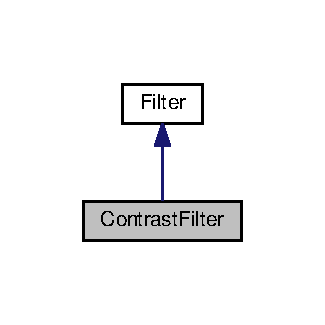
\includegraphics[width=156pt]{classModel_1_1ContrastFilter__inherit__graph}
\end{center}
\end{figure}
\subsection*{Public Member Functions}
\begin{DoxyCompactItemize}
\item 
\hyperlink{classModel_1_1ContrastFilter_abc944002d3dce00b176a4133c05f7c9c}{Contrast\+Filter} ()
\item 
void \hyperlink{classModel_1_1ContrastFilter_ac8255ffbc46bb61acaa8fd23d0d260eb}{set\+Intensity} (int \hyperlink{classModel_1_1ContrastFilter_a299ec0c42ccc5a2d79d1739428ac3210}{intensity})
\item 
int \hyperlink{classModel_1_1ContrastFilter_a708995fb1b6acb31ee0dfb0f4881e5b5}{get\+Intensity} ()
\item 
string \hyperlink{classModel_1_1ContrastFilter_a11335e13e50af74108bf926dc1340b4b}{get\+Name} ()
\item 
string \hyperlink{classModel_1_1ContrastFilter_a62b7b60e24f92234393b840b35808e06}{get\+Filter\+Description} ()
\end{DoxyCompactItemize}
\subsection*{Private Attributes}
\begin{DoxyCompactItemize}
\item 
int \hyperlink{classModel_1_1ContrastFilter_a299ec0c42ccc5a2d79d1739428ac3210}{intensity}
\end{DoxyCompactItemize}
\subsection*{Additional Inherited Members}


\subsection{Detailed Description}
Adjusts the contrast of the video. 

\subsection{Constructor \& Destructor Documentation}
\hypertarget{classModel_1_1ContrastFilter_abc944002d3dce00b176a4133c05f7c9c}{}\index{Model\+::\+Contrast\+Filter@{Model\+::\+Contrast\+Filter}!Contrast\+Filter@{Contrast\+Filter}}
\index{Contrast\+Filter@{Contrast\+Filter}!Model\+::\+Contrast\+Filter@{Model\+::\+Contrast\+Filter}}
\subsubsection[{Contrast\+Filter}]{\setlength{\rightskip}{0pt plus 5cm}{\bf Contrast\+Filter} (
\begin{DoxyParamCaption}
{}
\end{DoxyParamCaption}
)}\label{classModel_1_1ContrastFilter_abc944002d3dce00b176a4133c05f7c9c}


Constructor. 



\subsection{Member Function Documentation}
\hypertarget{classModel_1_1ContrastFilter_a62b7b60e24f92234393b840b35808e06}{}\index{Model\+::\+Contrast\+Filter@{Model\+::\+Contrast\+Filter}!get\+Filter\+Description@{get\+Filter\+Description}}
\index{get\+Filter\+Description@{get\+Filter\+Description}!Model\+::\+Contrast\+Filter@{Model\+::\+Contrast\+Filter}}
\subsubsection[{get\+Filter\+Description}]{\setlength{\rightskip}{0pt plus 5cm}string get\+Filter\+Description (
\begin{DoxyParamCaption}
{}
\end{DoxyParamCaption}
)\hspace{0.3cm}{\ttfamily [virtual]}}\label{classModel_1_1ContrastFilter_a62b7b60e24f92234393b840b35808e06}


Returns the string that the ffmpeg library needs to apply the filter to a video. 

\begin{DoxyReturn}{Returns}
The string for the ffmpeg library.
\end{DoxyReturn}


Implements \hyperlink{classModel_1_1Filter_a453fcafa809afa1ce58d9ef95d5f26c0}{Filter}.

\hypertarget{classModel_1_1ContrastFilter_a708995fb1b6acb31ee0dfb0f4881e5b5}{}\index{Model\+::\+Contrast\+Filter@{Model\+::\+Contrast\+Filter}!get\+Intensity@{get\+Intensity}}
\index{get\+Intensity@{get\+Intensity}!Model\+::\+Contrast\+Filter@{Model\+::\+Contrast\+Filter}}
\subsubsection[{get\+Intensity}]{\setlength{\rightskip}{0pt plus 5cm}int get\+Intensity (
\begin{DoxyParamCaption}
{}
\end{DoxyParamCaption}
)}\label{classModel_1_1ContrastFilter_a708995fb1b6acb31ee0dfb0f4881e5b5}


Returns the intensity of the contrast. 

\begin{DoxyReturn}{Returns}
The intensity.
\end{DoxyReturn}
\hypertarget{classModel_1_1ContrastFilter_a11335e13e50af74108bf926dc1340b4b}{}\index{Model\+::\+Contrast\+Filter@{Model\+::\+Contrast\+Filter}!get\+Name@{get\+Name}}
\index{get\+Name@{get\+Name}!Model\+::\+Contrast\+Filter@{Model\+::\+Contrast\+Filter}}
\subsubsection[{get\+Name}]{\setlength{\rightskip}{0pt plus 5cm}string get\+Name (
\begin{DoxyParamCaption}
{}
\end{DoxyParamCaption}
)\hspace{0.3cm}{\ttfamily [virtual]}}\label{classModel_1_1ContrastFilter_a11335e13e50af74108bf926dc1340b4b}


Returns the name of the filter. 

\begin{DoxyReturn}{Returns}
The filtername.
\end{DoxyReturn}


Implements \hyperlink{classModel_1_1Filter_ade93aa98c68d185a9c03784d36140225}{Filter}.

\hypertarget{classModel_1_1ContrastFilter_ac8255ffbc46bb61acaa8fd23d0d260eb}{}\index{Model\+::\+Contrast\+Filter@{Model\+::\+Contrast\+Filter}!set\+Intensity@{set\+Intensity}}
\index{set\+Intensity@{set\+Intensity}!Model\+::\+Contrast\+Filter@{Model\+::\+Contrast\+Filter}}
\subsubsection[{set\+Intensity}]{\setlength{\rightskip}{0pt plus 5cm}void set\+Intensity (
\begin{DoxyParamCaption}
\item[{int}]{intensity}
\end{DoxyParamCaption}
)}\label{classModel_1_1ContrastFilter_ac8255ffbc46bb61acaa8fd23d0d260eb}


Sets the intensity of the contrast. 


\begin{DoxyParams}{Parameters}
{\em intensity} & The new intensity.\\
\hline
\end{DoxyParams}


\subsection{Field Documentation}
\hypertarget{classModel_1_1ContrastFilter_a299ec0c42ccc5a2d79d1739428ac3210}{}\index{Model\+::\+Contrast\+Filter@{Model\+::\+Contrast\+Filter}!intensity@{intensity}}
\index{intensity@{intensity}!Model\+::\+Contrast\+Filter@{Model\+::\+Contrast\+Filter}}
\subsubsection[{intensity}]{\setlength{\rightskip}{0pt plus 5cm}int intensity\hspace{0.3cm}{\ttfamily [private]}}\label{classModel_1_1ContrastFilter_a299ec0c42ccc5a2d79d1739428ac3210}

\newpage\hypertarget{classGUI_1_1ContrastFilterBox}{}\section{Contrast\+Filter\+Box Class Reference}
\label{classGUI_1_1ContrastFilterBox}\index{Contrast\+Filter\+Box@{Contrast\+Filter\+Box}}


Inheritance diagram for Contrast\+Filter\+Box\+:
\nopagebreak
\begin{figure}[H]
\begin{center}
\leavevmode
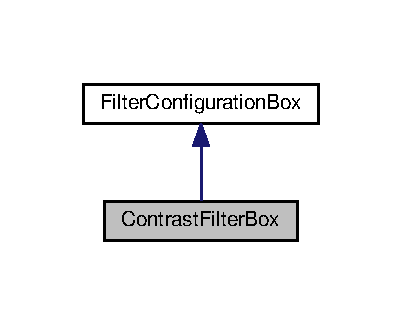
\includegraphics[width=193pt]{classGUI_1_1ContrastFilterBox__inherit__graph}
\end{center}
\end{figure}
\subsection*{Public Member Functions}
\begin{DoxyCompactItemize}
\item 
\hyperlink{classGUI_1_1ContrastFilterBox_a45a3637c1d2008b5631ae24e2419be1d}{Contrast\+Filter\+Box} (\hyperlink{classGUI_1_1QWidget}{G\+U\+I\+::\+Q\+Widget} $\ast$parent)
\end{DoxyCompactItemize}
\subsection*{Additional Inherited Members}


\subsection{Detailed Description}
This class contains the gui elements for changing the options of a contrast filter. 

\subsection{Constructor \& Destructor Documentation}
\hypertarget{classGUI_1_1ContrastFilterBox_a45a3637c1d2008b5631ae24e2419be1d}{}\index{G\+U\+I\+::\+Contrast\+Filter\+Box@{G\+U\+I\+::\+Contrast\+Filter\+Box}!Contrast\+Filter\+Box@{Contrast\+Filter\+Box}}
\index{Contrast\+Filter\+Box@{Contrast\+Filter\+Box}!G\+U\+I\+::\+Contrast\+Filter\+Box@{G\+U\+I\+::\+Contrast\+Filter\+Box}}
\subsubsection[{Contrast\+Filter\+Box}]{\setlength{\rightskip}{0pt plus 5cm}{\bf Contrast\+Filter\+Box} (
\begin{DoxyParamCaption}
\item[{{\bf G\+U\+I\+::\+Q\+Widget} $\ast$}]{parent}
\end{DoxyParamCaption}
)}\label{classGUI_1_1ContrastFilterBox_a45a3637c1d2008b5631ae24e2419be1d}


Constructor. 


\newpage\hypertarget{classGUI_1_1ControlPanel}{}\section{Control\+Panel Class Reference}
\label{classGUI_1_1ControlPanel}\index{Control\+Panel@{Control\+Panel}}


Inheritance diagram for Control\+Panel\+:
\nopagebreak
\begin{figure}[H]
\begin{center}
\leavevmode
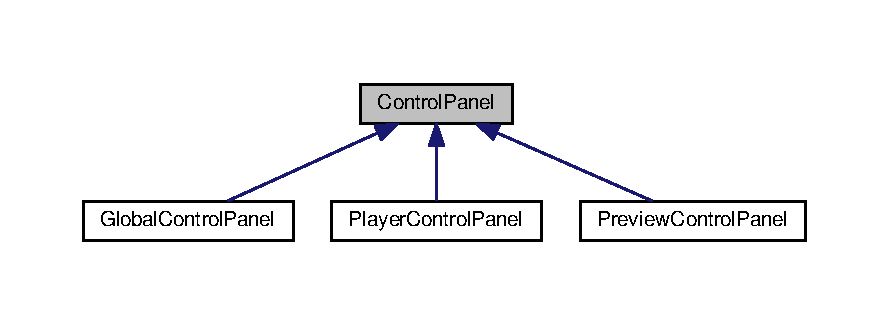
\includegraphics[width=350pt]{classGUI_1_1ControlPanel__inherit__graph}
\end{center}
\end{figure}
\subsection*{Public Member Functions}
\begin{DoxyCompactItemize}
\item 
\hyperlink{classGUI_1_1ControlPanel_a0efa607fe77b973e1128eae3bb33a9a1}{Control\+Panel} ()
\item 
void \hyperlink{classGUI_1_1ControlPanel_a798f5ffd7fe32e3fe8f67feed1e555c4}{set\+Master\+Video\+Player} (Player\+::\+Player \&player)
\item 
void \hyperlink{classGUI_1_1ControlPanel_a1a372b46dee9c1f2b2696337231b3add}{add\+Video\+Player} (\hyperlink{classGUI_1_1Player}{G\+U\+I\+::\+Player} \&player)
\item 
virtual void \hyperlink{classGUI_1_1ControlPanel_aa9963358cf9cff5ea2531d73efa78f73}{update\+Ui} ()=0
\item 
void \hyperlink{classGUI_1_1ControlPanel_aa24579c43e90697b0b05662270dfca3f}{remove\+Video\+Player} (Player\+::\+Player \&player)
\end{DoxyCompactItemize}
\subsection*{Data Fields}
\begin{DoxyCompactItemize}
\item 
\hyperlink{classGUI_1_1ForwardPlayer}{G\+U\+I\+::\+Forward\+Player} $\ast$ \hyperlink{classGUI_1_1ControlPanel_a15dc5e66f941f96f5b10d4da627f7f4e}{forward\+Panel}
\item 
\hyperlink{classGUI_1_1VideoPlayer}{G\+U\+I\+::\+Video\+Player} $\ast$ \hyperlink{classGUI_1_1ControlPanel_a5e72764e084c40951f89250eea333664}{master\+Panel}
\end{DoxyCompactItemize}
\subsection*{Protected Attributes}
\begin{DoxyCompactItemize}
\item 
std\+::vector$<$ \hyperlink{classGUI_1_1VideoPlayer}{G\+U\+I\+::\+Video\+Player} $\ast$ $>$ \hyperlink{classGUI_1_1ControlPanel_a5a284ea6859626e5d7ffb80231e5d319}{players}
\end{DoxyCompactItemize}
\subsection*{Private Attributes}
\begin{DoxyCompactItemize}
\item 
\hyperlink{classGUI_1_1Player}{G\+U\+I\+::\+Player} $\ast$ \hyperlink{classGUI_1_1ControlPanel_a32f716e694e82571b2bcf3159a1f2876}{master\+Player}
\end{DoxyCompactItemize}


\subsection{Detailed Description}
This class is the base class for control panels. Control panels control videoplayers, 

\subsection{Constructor \& Destructor Documentation}
\hypertarget{classGUI_1_1ControlPanel_a0efa607fe77b973e1128eae3bb33a9a1}{}\index{G\+U\+I\+::\+Control\+Panel@{G\+U\+I\+::\+Control\+Panel}!Control\+Panel@{Control\+Panel}}
\index{Control\+Panel@{Control\+Panel}!G\+U\+I\+::\+Control\+Panel@{G\+U\+I\+::\+Control\+Panel}}
\subsubsection[{Control\+Panel}]{\setlength{\rightskip}{0pt plus 5cm}{\bf Control\+Panel} (
\begin{DoxyParamCaption}
{}
\end{DoxyParamCaption}
)}\label{classGUI_1_1ControlPanel_a0efa607fe77b973e1128eae3bb33a9a1}


Constructor. 



\subsection{Member Function Documentation}
\hypertarget{classGUI_1_1ControlPanel_a1a372b46dee9c1f2b2696337231b3add}{}\index{G\+U\+I\+::\+Control\+Panel@{G\+U\+I\+::\+Control\+Panel}!add\+Video\+Player@{add\+Video\+Player}}
\index{add\+Video\+Player@{add\+Video\+Player}!G\+U\+I\+::\+Control\+Panel@{G\+U\+I\+::\+Control\+Panel}}
\subsubsection[{add\+Video\+Player}]{\setlength{\rightskip}{0pt plus 5cm}void add\+Video\+Player (
\begin{DoxyParamCaption}
\item[{{\bf G\+U\+I\+::\+Player} \&}]{player}
\end{DoxyParamCaption}
)}\label{classGUI_1_1ControlPanel_a1a372b46dee9c1f2b2696337231b3add}


Adds the video player the list of players to notify. 


\begin{DoxyParams}{Parameters}
{\em player} & The player to add to the list.\\
\hline
\end{DoxyParams}
\hypertarget{classGUI_1_1ControlPanel_aa24579c43e90697b0b05662270dfca3f}{}\index{G\+U\+I\+::\+Control\+Panel@{G\+U\+I\+::\+Control\+Panel}!remove\+Video\+Player@{remove\+Video\+Player}}
\index{remove\+Video\+Player@{remove\+Video\+Player}!G\+U\+I\+::\+Control\+Panel@{G\+U\+I\+::\+Control\+Panel}}
\subsubsection[{remove\+Video\+Player}]{\setlength{\rightskip}{0pt plus 5cm}void remove\+Video\+Player (
\begin{DoxyParamCaption}
\item[{Player\+::\+Player \&}]{player}
\end{DoxyParamCaption}
)}\label{classGUI_1_1ControlPanel_aa24579c43e90697b0b05662270dfca3f}


Removes the video player from the list of the players to notify. 


\begin{DoxyParams}{Parameters}
{\em player} & The player to remove.\\
\hline
\end{DoxyParams}
\hypertarget{classGUI_1_1ControlPanel_a798f5ffd7fe32e3fe8f67feed1e555c4}{}\index{G\+U\+I\+::\+Control\+Panel@{G\+U\+I\+::\+Control\+Panel}!set\+Master\+Video\+Player@{set\+Master\+Video\+Player}}
\index{set\+Master\+Video\+Player@{set\+Master\+Video\+Player}!G\+U\+I\+::\+Control\+Panel@{G\+U\+I\+::\+Control\+Panel}}
\subsubsection[{set\+Master\+Video\+Player}]{\setlength{\rightskip}{0pt plus 5cm}void set\+Master\+Video\+Player (
\begin{DoxyParamCaption}
\item[{Player\+::\+Player \&}]{player}
\end{DoxyParamCaption}
)}\label{classGUI_1_1ControlPanel_a798f5ffd7fe32e3fe8f67feed1e555c4}


Sets the master video player. The master video player is the reference to where to set the position of the slider, if the video is played paused or stopped. 


\begin{DoxyParams}{Parameters}
{\em player} & The master video player.\\
\hline
\end{DoxyParams}
\hypertarget{classGUI_1_1ControlPanel_aa9963358cf9cff5ea2531d73efa78f73}{}\index{G\+U\+I\+::\+Control\+Panel@{G\+U\+I\+::\+Control\+Panel}!update\+Ui@{update\+Ui}}
\index{update\+Ui@{update\+Ui}!G\+U\+I\+::\+Control\+Panel@{G\+U\+I\+::\+Control\+Panel}}
\subsubsection[{update\+Ui}]{\setlength{\rightskip}{0pt plus 5cm}virtual void update\+Ui (
\begin{DoxyParamCaption}
{}
\end{DoxyParamCaption}
)\hspace{0.3cm}{\ttfamily [pure virtual]}}\label{classGUI_1_1ControlPanel_aa9963358cf9cff5ea2531d73efa78f73}


Updates the ui of the control panel. 



Implemented in \hyperlink{classGUI_1_1PlayerControlPanel_ae13c7f95f1ceda0fec18d18c3d7619f6}{Player\+Control\+Panel}, \hyperlink{classGUI_1_1PreviewControlPanel_ae13c7f95f1ceda0fec18d18c3d7619f6}{Preview\+Control\+Panel}, and \hyperlink{classGUI_1_1GlobalControlPanel_ae13c7f95f1ceda0fec18d18c3d7619f6}{Global\+Control\+Panel}.



\subsection{Field Documentation}
\hypertarget{classGUI_1_1ControlPanel_a15dc5e66f941f96f5b10d4da627f7f4e}{}\index{G\+U\+I\+::\+Control\+Panel@{G\+U\+I\+::\+Control\+Panel}!forward\+Panel@{forward\+Panel}}
\index{forward\+Panel@{forward\+Panel}!G\+U\+I\+::\+Control\+Panel@{G\+U\+I\+::\+Control\+Panel}}
\subsubsection[{forward\+Panel}]{\setlength{\rightskip}{0pt plus 5cm}{\bf G\+U\+I\+::\+Forward\+Player}$\ast$ forward\+Panel}\label{classGUI_1_1ControlPanel_a15dc5e66f941f96f5b10d4da627f7f4e}
\hypertarget{classGUI_1_1ControlPanel_a5e72764e084c40951f89250eea333664}{}\index{G\+U\+I\+::\+Control\+Panel@{G\+U\+I\+::\+Control\+Panel}!master\+Panel@{master\+Panel}}
\index{master\+Panel@{master\+Panel}!G\+U\+I\+::\+Control\+Panel@{G\+U\+I\+::\+Control\+Panel}}
\subsubsection[{master\+Panel}]{\setlength{\rightskip}{0pt plus 5cm}{\bf G\+U\+I\+::\+Video\+Player}$\ast$ master\+Panel}\label{classGUI_1_1ControlPanel_a5e72764e084c40951f89250eea333664}
\hypertarget{classGUI_1_1ControlPanel_a32f716e694e82571b2bcf3159a1f2876}{}\index{G\+U\+I\+::\+Control\+Panel@{G\+U\+I\+::\+Control\+Panel}!master\+Player@{master\+Player}}
\index{master\+Player@{master\+Player}!G\+U\+I\+::\+Control\+Panel@{G\+U\+I\+::\+Control\+Panel}}
\subsubsection[{master\+Player}]{\setlength{\rightskip}{0pt plus 5cm}{\bf G\+U\+I\+::\+Player}$\ast$ master\+Player\hspace{0.3cm}{\ttfamily [private]}}\label{classGUI_1_1ControlPanel_a32f716e694e82571b2bcf3159a1f2876}
\hypertarget{classGUI_1_1ControlPanel_a5a284ea6859626e5d7ffb80231e5d319}{}\index{G\+U\+I\+::\+Control\+Panel@{G\+U\+I\+::\+Control\+Panel}!players@{players}}
\index{players@{players}!G\+U\+I\+::\+Control\+Panel@{G\+U\+I\+::\+Control\+Panel}}
\subsubsection[{players}]{\setlength{\rightskip}{0pt plus 5cm}std\+::vector$<${\bf G\+U\+I\+::\+Video\+Player}$\ast$$>$ players\hspace{0.3cm}{\ttfamily [protected]}}\label{classGUI_1_1ControlPanel_a5a284ea6859626e5d7ffb80231e5d319}

\newpage\hypertarget{classModel_1_1EdgeFilter}{}\section{Edge\+Filter Class Reference}
\label{classModel_1_1EdgeFilter}\index{Edge\+Filter@{Edge\+Filter}}


Inheritance diagram for Edge\+Filter\+:
\nopagebreak
\begin{figure}[H]
\begin{center}
\leavevmode
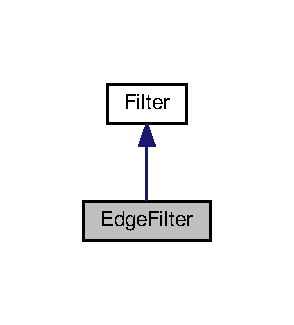
\includegraphics[width=141pt]{classModel_1_1EdgeFilter__inherit__graph}
\end{center}
\end{figure}
\subsection*{Public Member Functions}
\begin{DoxyCompactItemize}
\item 
\hyperlink{classModel_1_1EdgeFilter_a955edf58021ca1056d7b149c35bb829b}{Edge\+Filter} ()
\item 
string \hyperlink{classModel_1_1EdgeFilter_a62b7b60e24f92234393b840b35808e06}{get\+Filter\+Description} ()
\item 
string \hyperlink{classModel_1_1EdgeFilter_a11335e13e50af74108bf926dc1340b4b}{get\+Name} ()
\end{DoxyCompactItemize}
\subsection*{Additional Inherited Members}


\subsection{Detailed Description}
Filters everything but the edges out of the video. 

\subsection{Constructor \& Destructor Documentation}
\hypertarget{classModel_1_1EdgeFilter_a955edf58021ca1056d7b149c35bb829b}{}\index{Model\+::\+Edge\+Filter@{Model\+::\+Edge\+Filter}!Edge\+Filter@{Edge\+Filter}}
\index{Edge\+Filter@{Edge\+Filter}!Model\+::\+Edge\+Filter@{Model\+::\+Edge\+Filter}}
\subsubsection[{Edge\+Filter}]{\setlength{\rightskip}{0pt plus 5cm}{\bf Edge\+Filter} (
\begin{DoxyParamCaption}
{}
\end{DoxyParamCaption}
)}\label{classModel_1_1EdgeFilter_a955edf58021ca1056d7b149c35bb829b}


\subsection{Member Function Documentation}
\hypertarget{classModel_1_1EdgeFilter_a62b7b60e24f92234393b840b35808e06}{}\index{Model\+::\+Edge\+Filter@{Model\+::\+Edge\+Filter}!get\+Filter\+Description@{get\+Filter\+Description}}
\index{get\+Filter\+Description@{get\+Filter\+Description}!Model\+::\+Edge\+Filter@{Model\+::\+Edge\+Filter}}
\subsubsection[{get\+Filter\+Description}]{\setlength{\rightskip}{0pt plus 5cm}string get\+Filter\+Description (
\begin{DoxyParamCaption}
{}
\end{DoxyParamCaption}
)\hspace{0.3cm}{\ttfamily [virtual]}}\label{classModel_1_1EdgeFilter_a62b7b60e24f92234393b840b35808e06}


Returns the string that the ffmpeg library needs to apply the filter to a video. 

\begin{DoxyReturn}{Returns}
The string for the ffmpeg library.
\end{DoxyReturn}


Implements \hyperlink{classModel_1_1Filter_a453fcafa809afa1ce58d9ef95d5f26c0}{Filter}.

\hypertarget{classModel_1_1EdgeFilter_a11335e13e50af74108bf926dc1340b4b}{}\index{Model\+::\+Edge\+Filter@{Model\+::\+Edge\+Filter}!get\+Name@{get\+Name}}
\index{get\+Name@{get\+Name}!Model\+::\+Edge\+Filter@{Model\+::\+Edge\+Filter}}
\subsubsection[{get\+Name}]{\setlength{\rightskip}{0pt plus 5cm}string get\+Name (
\begin{DoxyParamCaption}
{}
\end{DoxyParamCaption}
)\hspace{0.3cm}{\ttfamily [virtual]}}\label{classModel_1_1EdgeFilter_a11335e13e50af74108bf926dc1340b4b}


Returns the name of the filter. 

\begin{DoxyReturn}{Returns}
The filtername.
\end{DoxyReturn}


Implements \hyperlink{classModel_1_1Filter_ade93aa98c68d185a9c03784d36140225}{Filter}.


\newpage\hypertarget{classModel_1_1EncodedVideo}{}\section{Encoded\+Video Class Reference}
\label{classModel_1_1EncodedVideo}\index{Encoded\+Video@{Encoded\+Video}}
\subsection*{Public Member Functions}
\begin{DoxyCompactItemize}
\item 
\hyperlink{classModel_1_1EncodedVideo_a436d811c3c2420e132a2b4e04959c5de}{Encoded\+Video} (Q\+String path)
\item 
Q\+String \hyperlink{classModel_1_1EncodedVideo_a1a94d0c9bf9dd725556721ac914025e3}{get\+Path} ()
\item 
int \hyperlink{classModel_1_1EncodedVideo_ac4465cfb146410e557acc4892afd9e7c}{get\+File\+Size} ()
\item 
int \hyperlink{classModel_1_1EncodedVideo_ab9202ba7e871cc8488f73a14e4e6abef}{get\+Number\+Of\+Colors} ()
\item 
Q\+String \hyperlink{classModel_1_1EncodedVideo_ad0b9ca84489c31d0155646495380ac0b}{get\+Codec} ()
\item 
\hyperlink{classModel_1_1Graph}{Model\+::\+Graph} \& \hyperlink{classModel_1_1EncodedVideo_afe6efbe8e2d7312d31f9df848685c2a1}{get\+Bitrate} ()
\item 
\hyperlink{classModel_1_1Graph}{Model\+::\+Graph} \& \hyperlink{classModel_1_1EncodedVideo_a4c4816fa0fc4d120b7ca4727f92b8434}{get\+Psnr} ()
\item 
\hyperlink{classModel_1_1Graph}{Model\+::\+Graph} \& \hyperlink{classModel_1_1EncodedVideo_a2e964007d3803c23555685e582f1f8f8}{get\+Red\+Histogramm} ()
\item 
\hyperlink{classModel_1_1Graph}{Model\+::\+Graph} \& \hyperlink{classModel_1_1EncodedVideo_a665006efad68684718c78c213e081f16}{get\+Blue\+Histogramm} ()
\item 
\hyperlink{classModel_1_1Graph}{Model\+::\+Graph} \& \hyperlink{classModel_1_1EncodedVideo_a85d21a1922c274ff928b8794627fc3f0}{get\+Green\+Histogramm} ()
\item 
\hyperlink{classModel_1_1AVVideo}{Model\+::\+A\+V\+Video} \& \hyperlink{classModel_1_1EncodedVideo_a58bd43e5cbaa711bf19b0c71efbc9834}{get\+Av\+Video} ()
\item 
\hyperlink{classGUI_1_1Player_1_1Video}{G\+U\+I\+::\+Player\+::\+Video} \& \hyperlink{classModel_1_1EncodedVideo_a8efa1486dd7b968e9b0f1cb5be919381}{get\+Macro\+Block\+Video} ()
\item 
\hyperlink{classGUI_1_1Player_1_1Video}{G\+U\+I\+::\+Player\+::\+Video} \& \hyperlink{classModel_1_1EncodedVideo_a85eb47f3e866632f0e48c89becc72d1a}{get\+Rgb\+Diff\+Video} (\hyperlink{classGUI_1_1Player_1_1Video}{G\+U\+I\+::\+Player\+::\+Video} $\ast$reference=0)
\item 
\hyperlink{classGUI_1_1Player_1_1Video}{G\+U\+I\+::\+Player\+::\+Video} \& \hyperlink{classModel_1_1EncodedVideo_a56ebcfcff7dfad1f4b9e302794451afe}{get\+Video} ()
\item 
void \hyperlink{classModel_1_1EncodedVideo_a60a6dd2db95a7b5512b119592154c542}{set\+Bitrate} (\hyperlink{classModel_1_1Graph}{Model\+::\+Graph} graph)
\item 
void \hyperlink{classModel_1_1EncodedVideo_a1ab9a88bf6af5d5c764512703becc453}{set\+Psnr} (\hyperlink{classModel_1_1Graph}{Model\+::\+Graph} graph)
\item 
void \hyperlink{classModel_1_1EncodedVideo_a50a774bf6d0a0445ad71fce4030f923b}{set\+Red\+Histogramm} (\hyperlink{classModel_1_1Graph}{Model\+::\+Graph} graph)
\item 
void \hyperlink{classModel_1_1EncodedVideo_a566ac8c5c38d5e9ff92033d425ad1af5}{set\+Green\+Histogramm} (\hyperlink{classModel_1_1Graph}{Model\+::\+Graph} graph)
\item 
void \hyperlink{classModel_1_1EncodedVideo_a73e0e302836a23164bc5fafc2efcb412}{set\+Blue\+Histogramm} (\hyperlink{classModel_1_1Graph}{Model\+::\+Graph} graph)
\item 
void \hyperlink{classModel_1_1EncodedVideo_aa7f8f6cccdf2b783931981c42c093fe5}{set\+Macroblock\+Video} (\hyperlink{classGUI_1_1Player_1_1Video}{G\+U\+I\+::\+Player\+::\+Video} \hyperlink{classModel_1_1EncodedVideo_a03e0f42a43f7a856dd9881df4024fb4c}{video})
\item 
void \hyperlink{classModel_1_1EncodedVideo_a9f858252aac3af726c1ba68f580321f9}{set\+Rgb\+Diff\+Video} (\hyperlink{classGUI_1_1Player_1_1Video}{G\+U\+I\+::\+Player\+::\+Video} \hyperlink{classModel_1_1EncodedVideo_a03e0f42a43f7a856dd9881df4024fb4c}{video})
\end{DoxyCompactItemize}
\subsection*{Data Fields}
\begin{DoxyCompactItemize}
\item 
\hyperlink{classGUI_1_1AnalysisBox}{G\+U\+I\+::\+Analysis\+Box} $\ast$ \hyperlink{classModel_1_1EncodedVideo_a03e0f42a43f7a856dd9881df4024fb4c}{video}
\item 
\hyperlink{classModel_1_1AVVideo}{Model\+::\+A\+V\+Video} $\ast$ \hyperlink{classModel_1_1EncodedVideo_a270efc836b2d2c70aec72106128ff89f}{av\+Video}
\item 
\hyperlink{classGUI_1_1Player_1_1Video}{G\+U\+I\+::\+Player\+::\+Video} $\ast$ \hyperlink{classModel_1_1EncodedVideo_a17f257b55491782940deb4e086adecbb}{display\+Video}
\item 
\hyperlink{classGUI_1_1Player_1_1Video}{G\+U\+I\+::\+Player\+::\+Video} $\ast$ \hyperlink{classModel_1_1EncodedVideo_afb2db9bff47ddb8b0d279068e7b24444}{macroblock\+Video}
\item 
\hyperlink{classGUI_1_1Player_1_1Video}{G\+U\+I\+::\+Player\+::\+Video} $\ast$ \hyperlink{classModel_1_1EncodedVideo_a0a3659e25658447f14c6c00399888369}{rgb\+Diff\+Video}
\item 
\hyperlink{classModel_1_1Graph}{Model\+::\+Graph} $\ast$ \hyperlink{classModel_1_1EncodedVideo_aec2e020f785ceb00064fb8033826603e}{bitrate}
\item 
\hyperlink{classModel_1_1Graph}{Model\+::\+Graph} $\ast$ \hyperlink{classModel_1_1EncodedVideo_a9bac82e3934ef7816be95e35cd18c852}{psnr}
\item 
\hyperlink{classModel_1_1Graph}{Model\+::\+Graph} $\ast$ \hyperlink{classModel_1_1EncodedVideo_a687c8a2518054613e946c48f33520458}{red\+Histo}
\item 
\hyperlink{classModel_1_1Graph}{Model\+::\+Graph} $\ast$ \hyperlink{classModel_1_1EncodedVideo_af09ff3f1ad12186cc33f3ab4cb146cdb}{green\+Histo}
\item 
\hyperlink{classModel_1_1Graph}{Model\+::\+Graph} $\ast$ \hyperlink{classModel_1_1EncodedVideo_a53ce36c444026a777d53d7c2d872b059}{blue\+Hiso}
\end{DoxyCompactItemize}


\subsection{Detailed Description}
This class contains all analysis info of a encoded video. 

\subsection{Constructor \& Destructor Documentation}
\hypertarget{classModel_1_1EncodedVideo_a436d811c3c2420e132a2b4e04959c5de}{}\index{Model\+::\+Encoded\+Video@{Model\+::\+Encoded\+Video}!Encoded\+Video@{Encoded\+Video}}
\index{Encoded\+Video@{Encoded\+Video}!Model\+::\+Encoded\+Video@{Model\+::\+Encoded\+Video}}
\subsubsection[{Encoded\+Video}]{\setlength{\rightskip}{0pt plus 5cm}{\bf Encoded\+Video} (
\begin{DoxyParamCaption}
\item[{Q\+String}]{path}
\end{DoxyParamCaption}
)}\label{classModel_1_1EncodedVideo_a436d811c3c2420e132a2b4e04959c5de}


Constructor. 


\begin{DoxyParams}{Parameters}
{\em path} & Path to the video.\\
\hline
\end{DoxyParams}


\subsection{Member Function Documentation}
\hypertarget{classModel_1_1EncodedVideo_a58bd43e5cbaa711bf19b0c71efbc9834}{}\index{Model\+::\+Encoded\+Video@{Model\+::\+Encoded\+Video}!get\+Av\+Video@{get\+Av\+Video}}
\index{get\+Av\+Video@{get\+Av\+Video}!Model\+::\+Encoded\+Video@{Model\+::\+Encoded\+Video}}
\subsubsection[{get\+Av\+Video}]{\setlength{\rightskip}{0pt plus 5cm}{\bf Model\+::\+A\+V\+Video} \& get\+Av\+Video (
\begin{DoxyParamCaption}
{}
\end{DoxyParamCaption}
)}\label{classModel_1_1EncodedVideo_a58bd43e5cbaa711bf19b0c71efbc9834}


Returns the \hyperlink{classModel_1_1AVVideo}{A\+V\+Video}. 

\begin{DoxyReturn}{Returns}
The \hyperlink{classModel_1_1AVVideo}{A\+V\+Video}.
\end{DoxyReturn}
\hypertarget{classModel_1_1EncodedVideo_afe6efbe8e2d7312d31f9df848685c2a1}{}\index{Model\+::\+Encoded\+Video@{Model\+::\+Encoded\+Video}!get\+Bitrate@{get\+Bitrate}}
\index{get\+Bitrate@{get\+Bitrate}!Model\+::\+Encoded\+Video@{Model\+::\+Encoded\+Video}}
\subsubsection[{get\+Bitrate}]{\setlength{\rightskip}{0pt plus 5cm}{\bf Model\+::\+Graph} \& get\+Bitrate (
\begin{DoxyParamCaption}
{}
\end{DoxyParamCaption}
)}\label{classModel_1_1EncodedVideo_afe6efbe8e2d7312d31f9df848685c2a1}


Returns the bitrate graph. 

\begin{DoxyReturn}{Returns}
The bitrate graph.
\end{DoxyReturn}
\hypertarget{classModel_1_1EncodedVideo_a665006efad68684718c78c213e081f16}{}\index{Model\+::\+Encoded\+Video@{Model\+::\+Encoded\+Video}!get\+Blue\+Histogramm@{get\+Blue\+Histogramm}}
\index{get\+Blue\+Histogramm@{get\+Blue\+Histogramm}!Model\+::\+Encoded\+Video@{Model\+::\+Encoded\+Video}}
\subsubsection[{get\+Blue\+Histogramm}]{\setlength{\rightskip}{0pt plus 5cm}{\bf Model\+::\+Graph} \& get\+Blue\+Histogramm (
\begin{DoxyParamCaption}
{}
\end{DoxyParamCaption}
)}\label{classModel_1_1EncodedVideo_a665006efad68684718c78c213e081f16}


Returns the blue histogramm graph. 

\begin{DoxyReturn}{Returns}
The blue histogramm.
\end{DoxyReturn}
\hypertarget{classModel_1_1EncodedVideo_ad0b9ca84489c31d0155646495380ac0b}{}\index{Model\+::\+Encoded\+Video@{Model\+::\+Encoded\+Video}!get\+Codec@{get\+Codec}}
\index{get\+Codec@{get\+Codec}!Model\+::\+Encoded\+Video@{Model\+::\+Encoded\+Video}}
\subsubsection[{get\+Codec}]{\setlength{\rightskip}{0pt plus 5cm}Q\+String get\+Codec (
\begin{DoxyParamCaption}
{}
\end{DoxyParamCaption}
)}\label{classModel_1_1EncodedVideo_ad0b9ca84489c31d0155646495380ac0b}


Returns the codec used in the video file. 

\begin{DoxyReturn}{Returns}
The used codec.
\end{DoxyReturn}
\hypertarget{classModel_1_1EncodedVideo_ac4465cfb146410e557acc4892afd9e7c}{}\index{Model\+::\+Encoded\+Video@{Model\+::\+Encoded\+Video}!get\+File\+Size@{get\+File\+Size}}
\index{get\+File\+Size@{get\+File\+Size}!Model\+::\+Encoded\+Video@{Model\+::\+Encoded\+Video}}
\subsubsection[{get\+File\+Size}]{\setlength{\rightskip}{0pt plus 5cm}int get\+File\+Size (
\begin{DoxyParamCaption}
{}
\end{DoxyParamCaption}
)}\label{classModel_1_1EncodedVideo_ac4465cfb146410e557acc4892afd9e7c}


Returns the size of the video file. 

\begin{DoxyReturn}{Returns}
the file size.
\end{DoxyReturn}
\hypertarget{classModel_1_1EncodedVideo_a85d21a1922c274ff928b8794627fc3f0}{}\index{Model\+::\+Encoded\+Video@{Model\+::\+Encoded\+Video}!get\+Green\+Histogramm@{get\+Green\+Histogramm}}
\index{get\+Green\+Histogramm@{get\+Green\+Histogramm}!Model\+::\+Encoded\+Video@{Model\+::\+Encoded\+Video}}
\subsubsection[{get\+Green\+Histogramm}]{\setlength{\rightskip}{0pt plus 5cm}{\bf Model\+::\+Graph} \& get\+Green\+Histogramm (
\begin{DoxyParamCaption}
{}
\end{DoxyParamCaption}
)}\label{classModel_1_1EncodedVideo_a85d21a1922c274ff928b8794627fc3f0}


Returns the green histogramm graph. 

\begin{DoxyReturn}{Returns}
The green histogramm.
\end{DoxyReturn}
\hypertarget{classModel_1_1EncodedVideo_a8efa1486dd7b968e9b0f1cb5be919381}{}\index{Model\+::\+Encoded\+Video@{Model\+::\+Encoded\+Video}!get\+Macro\+Block\+Video@{get\+Macro\+Block\+Video}}
\index{get\+Macro\+Block\+Video@{get\+Macro\+Block\+Video}!Model\+::\+Encoded\+Video@{Model\+::\+Encoded\+Video}}
\subsubsection[{get\+Macro\+Block\+Video}]{\setlength{\rightskip}{0pt plus 5cm}{\bf G\+U\+I\+::\+Player\+::\+Video} \& get\+Macro\+Block\+Video (
\begin{DoxyParamCaption}
{}
\end{DoxyParamCaption}
)}\label{classModel_1_1EncodedVideo_a8efa1486dd7b968e9b0f1cb5be919381}


Returns the video which shows the macroblocks. 

\begin{DoxyReturn}{Returns}
The macroblock video.
\end{DoxyReturn}
\hypertarget{classModel_1_1EncodedVideo_ab9202ba7e871cc8488f73a14e4e6abef}{}\index{Model\+::\+Encoded\+Video@{Model\+::\+Encoded\+Video}!get\+Number\+Of\+Colors@{get\+Number\+Of\+Colors}}
\index{get\+Number\+Of\+Colors@{get\+Number\+Of\+Colors}!Model\+::\+Encoded\+Video@{Model\+::\+Encoded\+Video}}
\subsubsection[{get\+Number\+Of\+Colors}]{\setlength{\rightskip}{0pt plus 5cm}int get\+Number\+Of\+Colors (
\begin{DoxyParamCaption}
{}
\end{DoxyParamCaption}
)}\label{classModel_1_1EncodedVideo_ab9202ba7e871cc8488f73a14e4e6abef}


Returns the number of colors that appear in the whole video. 

\begin{DoxyReturn}{Returns}
The number of colors in the video.
\end{DoxyReturn}
\hypertarget{classModel_1_1EncodedVideo_a1a94d0c9bf9dd725556721ac914025e3}{}\index{Model\+::\+Encoded\+Video@{Model\+::\+Encoded\+Video}!get\+Path@{get\+Path}}
\index{get\+Path@{get\+Path}!Model\+::\+Encoded\+Video@{Model\+::\+Encoded\+Video}}
\subsubsection[{get\+Path}]{\setlength{\rightskip}{0pt plus 5cm}Q\+String get\+Path (
\begin{DoxyParamCaption}
{}
\end{DoxyParamCaption}
)}\label{classModel_1_1EncodedVideo_a1a94d0c9bf9dd725556721ac914025e3}


Returns the path to the video. 

\begin{DoxyReturn}{Returns}
The path to the video.
\end{DoxyReturn}
\hypertarget{classModel_1_1EncodedVideo_a4c4816fa0fc4d120b7ca4727f92b8434}{}\index{Model\+::\+Encoded\+Video@{Model\+::\+Encoded\+Video}!get\+Psnr@{get\+Psnr}}
\index{get\+Psnr@{get\+Psnr}!Model\+::\+Encoded\+Video@{Model\+::\+Encoded\+Video}}
\subsubsection[{get\+Psnr}]{\setlength{\rightskip}{0pt plus 5cm}{\bf Model\+::\+Graph} \& get\+Psnr (
\begin{DoxyParamCaption}
{}
\end{DoxyParamCaption}
)}\label{classModel_1_1EncodedVideo_a4c4816fa0fc4d120b7ca4727f92b8434}


Returns the psnr graph. 

\begin{DoxyReturn}{Returns}
The psnr graph.
\end{DoxyReturn}
\hypertarget{classModel_1_1EncodedVideo_a2e964007d3803c23555685e582f1f8f8}{}\index{Model\+::\+Encoded\+Video@{Model\+::\+Encoded\+Video}!get\+Red\+Histogramm@{get\+Red\+Histogramm}}
\index{get\+Red\+Histogramm@{get\+Red\+Histogramm}!Model\+::\+Encoded\+Video@{Model\+::\+Encoded\+Video}}
\subsubsection[{get\+Red\+Histogramm}]{\setlength{\rightskip}{0pt plus 5cm}{\bf Model\+::\+Graph} \& get\+Red\+Histogramm (
\begin{DoxyParamCaption}
{}
\end{DoxyParamCaption}
)}\label{classModel_1_1EncodedVideo_a2e964007d3803c23555685e582f1f8f8}


Returns the red histogramm graph. 

\begin{DoxyReturn}{Returns}
The red histogramm.
\end{DoxyReturn}
\hypertarget{classModel_1_1EncodedVideo_a85eb47f3e866632f0e48c89becc72d1a}{}\index{Model\+::\+Encoded\+Video@{Model\+::\+Encoded\+Video}!get\+Rgb\+Diff\+Video@{get\+Rgb\+Diff\+Video}}
\index{get\+Rgb\+Diff\+Video@{get\+Rgb\+Diff\+Video}!Model\+::\+Encoded\+Video@{Model\+::\+Encoded\+Video}}
\subsubsection[{get\+Rgb\+Diff\+Video}]{\setlength{\rightskip}{0pt plus 5cm}{\bf G\+U\+I\+::\+Player\+::\+Video} \& get\+Rgb\+Diff\+Video (
\begin{DoxyParamCaption}
\item[{{\bf G\+U\+I\+::\+Player\+::\+Video} $\ast$}]{reference = {\ttfamily 0}}
\end{DoxyParamCaption}
)}\label{classModel_1_1EncodedVideo_a85eb47f3e866632f0e48c89becc72d1a}


Returns the video which shows the rgb difference to another video. 


\begin{DoxyParams}{Parameters}
{\em reference} & The video to compare to.\\
\hline
\end{DoxyParams}
\begin{DoxyReturn}{Returns}
The rgb diff video.
\end{DoxyReturn}
\hypertarget{classModel_1_1EncodedVideo_a56ebcfcff7dfad1f4b9e302794451afe}{}\index{Model\+::\+Encoded\+Video@{Model\+::\+Encoded\+Video}!get\+Video@{get\+Video}}
\index{get\+Video@{get\+Video}!Model\+::\+Encoded\+Video@{Model\+::\+Encoded\+Video}}
\subsubsection[{get\+Video}]{\setlength{\rightskip}{0pt plus 5cm}{\bf G\+U\+I\+::\+Player\+::\+Video} \& get\+Video (
\begin{DoxyParamCaption}
{}
\end{DoxyParamCaption}
)}\label{classModel_1_1EncodedVideo_a56ebcfcff7dfad1f4b9e302794451afe}


Returns the Video. 

\begin{DoxyReturn}{Returns}
The Video.
\end{DoxyReturn}
\hypertarget{classModel_1_1EncodedVideo_a60a6dd2db95a7b5512b119592154c542}{}\index{Model\+::\+Encoded\+Video@{Model\+::\+Encoded\+Video}!set\+Bitrate@{set\+Bitrate}}
\index{set\+Bitrate@{set\+Bitrate}!Model\+::\+Encoded\+Video@{Model\+::\+Encoded\+Video}}
\subsubsection[{set\+Bitrate}]{\setlength{\rightskip}{0pt plus 5cm}void set\+Bitrate (
\begin{DoxyParamCaption}
\item[{{\bf Model\+::\+Graph}}]{graph}
\end{DoxyParamCaption}
)}\label{classModel_1_1EncodedVideo_a60a6dd2db95a7b5512b119592154c542}


Sets the bitrate graph. 


\begin{DoxyParams}{Parameters}
{\em graph} & The bitrate graph.\\
\hline
\end{DoxyParams}
\hypertarget{classModel_1_1EncodedVideo_a73e0e302836a23164bc5fafc2efcb412}{}\index{Model\+::\+Encoded\+Video@{Model\+::\+Encoded\+Video}!set\+Blue\+Histogramm@{set\+Blue\+Histogramm}}
\index{set\+Blue\+Histogramm@{set\+Blue\+Histogramm}!Model\+::\+Encoded\+Video@{Model\+::\+Encoded\+Video}}
\subsubsection[{set\+Blue\+Histogramm}]{\setlength{\rightskip}{0pt plus 5cm}void set\+Blue\+Histogramm (
\begin{DoxyParamCaption}
\item[{{\bf Model\+::\+Graph}}]{graph}
\end{DoxyParamCaption}
)}\label{classModel_1_1EncodedVideo_a73e0e302836a23164bc5fafc2efcb412}


Sets the blue histogramm graph. 


\begin{DoxyParams}{Parameters}
{\em graph} & The blue histogramm.\\
\hline
\end{DoxyParams}
\hypertarget{classModel_1_1EncodedVideo_a566ac8c5c38d5e9ff92033d425ad1af5}{}\index{Model\+::\+Encoded\+Video@{Model\+::\+Encoded\+Video}!set\+Green\+Histogramm@{set\+Green\+Histogramm}}
\index{set\+Green\+Histogramm@{set\+Green\+Histogramm}!Model\+::\+Encoded\+Video@{Model\+::\+Encoded\+Video}}
\subsubsection[{set\+Green\+Histogramm}]{\setlength{\rightskip}{0pt plus 5cm}void set\+Green\+Histogramm (
\begin{DoxyParamCaption}
\item[{{\bf Model\+::\+Graph}}]{graph}
\end{DoxyParamCaption}
)}\label{classModel_1_1EncodedVideo_a566ac8c5c38d5e9ff92033d425ad1af5}


Sets the green histogramm graph. 


\begin{DoxyParams}{Parameters}
{\em graph} & The green histogramm.\\
\hline
\end{DoxyParams}
\hypertarget{classModel_1_1EncodedVideo_aa7f8f6cccdf2b783931981c42c093fe5}{}\index{Model\+::\+Encoded\+Video@{Model\+::\+Encoded\+Video}!set\+Macroblock\+Video@{set\+Macroblock\+Video}}
\index{set\+Macroblock\+Video@{set\+Macroblock\+Video}!Model\+::\+Encoded\+Video@{Model\+::\+Encoded\+Video}}
\subsubsection[{set\+Macroblock\+Video}]{\setlength{\rightskip}{0pt plus 5cm}void set\+Macroblock\+Video (
\begin{DoxyParamCaption}
\item[{{\bf G\+U\+I\+::\+Player\+::\+Video}}]{video}
\end{DoxyParamCaption}
)}\label{classModel_1_1EncodedVideo_aa7f8f6cccdf2b783931981c42c093fe5}


Sets the video that shows the macroblocks. 


\begin{DoxyParams}{Parameters}
{\em video} & The macroblcok video.\\
\hline
\end{DoxyParams}
\hypertarget{classModel_1_1EncodedVideo_a1ab9a88bf6af5d5c764512703becc453}{}\index{Model\+::\+Encoded\+Video@{Model\+::\+Encoded\+Video}!set\+Psnr@{set\+Psnr}}
\index{set\+Psnr@{set\+Psnr}!Model\+::\+Encoded\+Video@{Model\+::\+Encoded\+Video}}
\subsubsection[{set\+Psnr}]{\setlength{\rightskip}{0pt plus 5cm}void set\+Psnr (
\begin{DoxyParamCaption}
\item[{{\bf Model\+::\+Graph}}]{graph}
\end{DoxyParamCaption}
)}\label{classModel_1_1EncodedVideo_a1ab9a88bf6af5d5c764512703becc453}


Sets the psnr graph. 


\begin{DoxyParams}{Parameters}
{\em graph} & The psnr graph.\\
\hline
\end{DoxyParams}
\hypertarget{classModel_1_1EncodedVideo_a50a774bf6d0a0445ad71fce4030f923b}{}\index{Model\+::\+Encoded\+Video@{Model\+::\+Encoded\+Video}!set\+Red\+Histogramm@{set\+Red\+Histogramm}}
\index{set\+Red\+Histogramm@{set\+Red\+Histogramm}!Model\+::\+Encoded\+Video@{Model\+::\+Encoded\+Video}}
\subsubsection[{set\+Red\+Histogramm}]{\setlength{\rightskip}{0pt plus 5cm}void set\+Red\+Histogramm (
\begin{DoxyParamCaption}
\item[{{\bf Model\+::\+Graph}}]{graph}
\end{DoxyParamCaption}
)}\label{classModel_1_1EncodedVideo_a50a774bf6d0a0445ad71fce4030f923b}


Sets the red histogramm graph. 


\begin{DoxyParams}{Parameters}
{\em graph} & The red histogramm.\\
\hline
\end{DoxyParams}
\hypertarget{classModel_1_1EncodedVideo_a9f858252aac3af726c1ba68f580321f9}{}\index{Model\+::\+Encoded\+Video@{Model\+::\+Encoded\+Video}!set\+Rgb\+Diff\+Video@{set\+Rgb\+Diff\+Video}}
\index{set\+Rgb\+Diff\+Video@{set\+Rgb\+Diff\+Video}!Model\+::\+Encoded\+Video@{Model\+::\+Encoded\+Video}}
\subsubsection[{set\+Rgb\+Diff\+Video}]{\setlength{\rightskip}{0pt plus 5cm}void set\+Rgb\+Diff\+Video (
\begin{DoxyParamCaption}
\item[{{\bf G\+U\+I\+::\+Player\+::\+Video}}]{video}
\end{DoxyParamCaption}
)}\label{classModel_1_1EncodedVideo_a9f858252aac3af726c1ba68f580321f9}


Sets the video that shows a rgb differenece to another video. 


\begin{DoxyParams}{Parameters}
{\em video} & The rgb diff video.\\
\hline
\end{DoxyParams}


\subsection{Field Documentation}
\hypertarget{classModel_1_1EncodedVideo_a270efc836b2d2c70aec72106128ff89f}{}\index{Model\+::\+Encoded\+Video@{Model\+::\+Encoded\+Video}!av\+Video@{av\+Video}}
\index{av\+Video@{av\+Video}!Model\+::\+Encoded\+Video@{Model\+::\+Encoded\+Video}}
\subsubsection[{av\+Video}]{\setlength{\rightskip}{0pt plus 5cm}{\bf Model\+::\+A\+V\+Video}$\ast$ av\+Video}\label{classModel_1_1EncodedVideo_a270efc836b2d2c70aec72106128ff89f}
\hypertarget{classModel_1_1EncodedVideo_aec2e020f785ceb00064fb8033826603e}{}\index{Model\+::\+Encoded\+Video@{Model\+::\+Encoded\+Video}!bitrate@{bitrate}}
\index{bitrate@{bitrate}!Model\+::\+Encoded\+Video@{Model\+::\+Encoded\+Video}}
\subsubsection[{bitrate}]{\setlength{\rightskip}{0pt plus 5cm}{\bf Model\+::\+Graph}$\ast$ bitrate}\label{classModel_1_1EncodedVideo_aec2e020f785ceb00064fb8033826603e}
\hypertarget{classModel_1_1EncodedVideo_a53ce36c444026a777d53d7c2d872b059}{}\index{Model\+::\+Encoded\+Video@{Model\+::\+Encoded\+Video}!blue\+Hiso@{blue\+Hiso}}
\index{blue\+Hiso@{blue\+Hiso}!Model\+::\+Encoded\+Video@{Model\+::\+Encoded\+Video}}
\subsubsection[{blue\+Hiso}]{\setlength{\rightskip}{0pt plus 5cm}{\bf Model\+::\+Graph}$\ast$ blue\+Hiso}\label{classModel_1_1EncodedVideo_a53ce36c444026a777d53d7c2d872b059}
\hypertarget{classModel_1_1EncodedVideo_a17f257b55491782940deb4e086adecbb}{}\index{Model\+::\+Encoded\+Video@{Model\+::\+Encoded\+Video}!display\+Video@{display\+Video}}
\index{display\+Video@{display\+Video}!Model\+::\+Encoded\+Video@{Model\+::\+Encoded\+Video}}
\subsubsection[{display\+Video}]{\setlength{\rightskip}{0pt plus 5cm}{\bf G\+U\+I\+::\+Player\+::\+Video}$\ast$ display\+Video}\label{classModel_1_1EncodedVideo_a17f257b55491782940deb4e086adecbb}
\hypertarget{classModel_1_1EncodedVideo_af09ff3f1ad12186cc33f3ab4cb146cdb}{}\index{Model\+::\+Encoded\+Video@{Model\+::\+Encoded\+Video}!green\+Histo@{green\+Histo}}
\index{green\+Histo@{green\+Histo}!Model\+::\+Encoded\+Video@{Model\+::\+Encoded\+Video}}
\subsubsection[{green\+Histo}]{\setlength{\rightskip}{0pt plus 5cm}{\bf Model\+::\+Graph}$\ast$ green\+Histo}\label{classModel_1_1EncodedVideo_af09ff3f1ad12186cc33f3ab4cb146cdb}
\hypertarget{classModel_1_1EncodedVideo_afb2db9bff47ddb8b0d279068e7b24444}{}\index{Model\+::\+Encoded\+Video@{Model\+::\+Encoded\+Video}!macroblock\+Video@{macroblock\+Video}}
\index{macroblock\+Video@{macroblock\+Video}!Model\+::\+Encoded\+Video@{Model\+::\+Encoded\+Video}}
\subsubsection[{macroblock\+Video}]{\setlength{\rightskip}{0pt plus 5cm}{\bf G\+U\+I\+::\+Player\+::\+Video}$\ast$ macroblock\+Video}\label{classModel_1_1EncodedVideo_afb2db9bff47ddb8b0d279068e7b24444}
\hypertarget{classModel_1_1EncodedVideo_a9bac82e3934ef7816be95e35cd18c852}{}\index{Model\+::\+Encoded\+Video@{Model\+::\+Encoded\+Video}!psnr@{psnr}}
\index{psnr@{psnr}!Model\+::\+Encoded\+Video@{Model\+::\+Encoded\+Video}}
\subsubsection[{psnr}]{\setlength{\rightskip}{0pt plus 5cm}{\bf Model\+::\+Graph}$\ast$ psnr}\label{classModel_1_1EncodedVideo_a9bac82e3934ef7816be95e35cd18c852}
\hypertarget{classModel_1_1EncodedVideo_a687c8a2518054613e946c48f33520458}{}\index{Model\+::\+Encoded\+Video@{Model\+::\+Encoded\+Video}!red\+Histo@{red\+Histo}}
\index{red\+Histo@{red\+Histo}!Model\+::\+Encoded\+Video@{Model\+::\+Encoded\+Video}}
\subsubsection[{red\+Histo}]{\setlength{\rightskip}{0pt plus 5cm}{\bf Model\+::\+Graph}$\ast$ red\+Histo}\label{classModel_1_1EncodedVideo_a687c8a2518054613e946c48f33520458}
\hypertarget{classModel_1_1EncodedVideo_a0a3659e25658447f14c6c00399888369}{}\index{Model\+::\+Encoded\+Video@{Model\+::\+Encoded\+Video}!rgb\+Diff\+Video@{rgb\+Diff\+Video}}
\index{rgb\+Diff\+Video@{rgb\+Diff\+Video}!Model\+::\+Encoded\+Video@{Model\+::\+Encoded\+Video}}
\subsubsection[{rgb\+Diff\+Video}]{\setlength{\rightskip}{0pt plus 5cm}{\bf G\+U\+I\+::\+Player\+::\+Video}$\ast$ rgb\+Diff\+Video}\label{classModel_1_1EncodedVideo_a0a3659e25658447f14c6c00399888369}
\hypertarget{classModel_1_1EncodedVideo_a03e0f42a43f7a856dd9881df4024fb4c}{}\index{Model\+::\+Encoded\+Video@{Model\+::\+Encoded\+Video}!video@{video}}
\index{video@{video}!Model\+::\+Encoded\+Video@{Model\+::\+Encoded\+Video}}
\subsubsection[{video}]{\setlength{\rightskip}{0pt plus 5cm}{\bf G\+U\+I\+::\+Analysis\+Box}$\ast$ video}\label{classModel_1_1EncodedVideo_a03e0f42a43f7a856dd9881df4024fb4c}

\newpage\hypertarget{classModel_1_1Filter}{}\section{Filter Class Reference}
\label{classModel_1_1Filter}\index{Filter@{Filter}}


Inheritance diagram for Filter\+:
\nopagebreak
\begin{figure}[H]
\begin{center}
\leavevmode
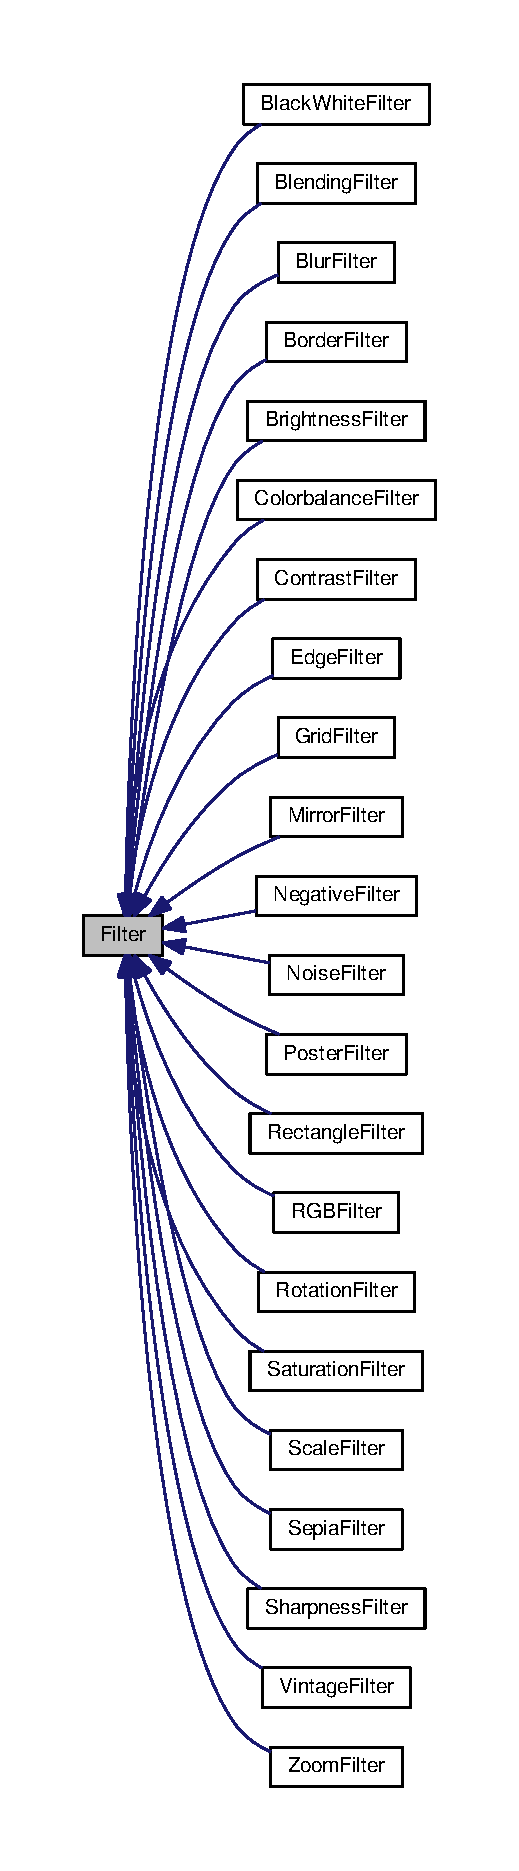
\includegraphics[height=550pt]{classModel_1_1Filter__inherit__graph}
\end{center}
\end{figure}
\subsection*{Public Member Functions}
\begin{DoxyCompactItemize}
\item 
virtual string \hyperlink{classModel_1_1Filter_a453fcafa809afa1ce58d9ef95d5f26c0}{get\+Filter\+Description} ()=0
\item 
virtual string \hyperlink{classModel_1_1Filter_ade93aa98c68d185a9c03784d36140225}{get\+Name} ()=0
\end{DoxyCompactItemize}
\subsection*{Data Fields}
\begin{DoxyCompactItemize}
\item 
\hyperlink{classUndoRedo_1_1RemoveFilter}{Undo\+Redo\+::\+Remove\+Filter} $\ast$ \hyperlink{classModel_1_1Filter_a380b5b271af99af20b25c1419b390130}{filter}
\end{DoxyCompactItemize}


\subsection{Detailed Description}
Baseclass for Filters. 

\subsection{Member Function Documentation}
\hypertarget{classModel_1_1Filter_a453fcafa809afa1ce58d9ef95d5f26c0}{}\index{Model\+::\+Filter@{Model\+::\+Filter}!get\+Filter\+Description@{get\+Filter\+Description}}
\index{get\+Filter\+Description@{get\+Filter\+Description}!Model\+::\+Filter@{Model\+::\+Filter}}
\subsubsection[{get\+Filter\+Description}]{\setlength{\rightskip}{0pt plus 5cm}virtual string get\+Filter\+Description (
\begin{DoxyParamCaption}
{}
\end{DoxyParamCaption}
)\hspace{0.3cm}{\ttfamily [pure virtual]}}\label{classModel_1_1Filter_a453fcafa809afa1ce58d9ef95d5f26c0}


Returns the string that the ffmpeg library needs to apply the filter to a video. 

\begin{DoxyReturn}{Returns}
The string for the ffmpeg library.
\end{DoxyReturn}


Implemented in \hyperlink{classModel_1_1BorderFilter_a62b7b60e24f92234393b840b35808e06}{Border\+Filter}, \hyperlink{classModel_1_1ColorbalanceFilter_a62b7b60e24f92234393b840b35808e06}{Colorbalance\+Filter}, \hyperlink{classModel_1_1BlendingFilter_a62b7b60e24f92234393b840b35808e06}{Blending\+Filter}, \hyperlink{classModel_1_1BlurFilter_a62b7b60e24f92234393b840b35808e06}{Blur\+Filter}, \hyperlink{classModel_1_1BrightnessFilter_a62b7b60e24f92234393b840b35808e06}{Brightness\+Filter}, \hyperlink{classModel_1_1ContrastFilter_a62b7b60e24f92234393b840b35808e06}{Contrast\+Filter}, \hyperlink{classModel_1_1RectangleFilter_a62b7b60e24f92234393b840b35808e06}{Rectangle\+Filter}, \hyperlink{classModel_1_1GridFilter_a62b7b60e24f92234393b840b35808e06}{Grid\+Filter}, \hyperlink{classModel_1_1NoiseFilter_a62b7b60e24f92234393b840b35808e06}{Noise\+Filter}, \hyperlink{classModel_1_1ScaleFilter_a62b7b60e24f92234393b840b35808e06}{Scale\+Filter}, \hyperlink{classModel_1_1MirrorFilter_a62b7b60e24f92234393b840b35808e06}{Mirror\+Filter}, \hyperlink{classModel_1_1RGBFilter_a62b7b60e24f92234393b840b35808e06}{R\+G\+B\+Filter}, \hyperlink{classModel_1_1ZoomFilter_a62b7b60e24f92234393b840b35808e06}{Zoom\+Filter}, \hyperlink{classModel_1_1BlackWhiteFilter_a62b7b60e24f92234393b840b35808e06}{Black\+White\+Filter}, \hyperlink{classModel_1_1PosterFilter_a62b7b60e24f92234393b840b35808e06}{Poster\+Filter}, \hyperlink{classModel_1_1RotationFilter_a62b7b60e24f92234393b840b35808e06}{Rotation\+Filter}, \hyperlink{classModel_1_1SaturationFilter_a62b7b60e24f92234393b840b35808e06}{Saturation\+Filter}, \hyperlink{classModel_1_1SharpnessFilter_a62b7b60e24f92234393b840b35808e06}{Sharpness\+Filter}, \hyperlink{classModel_1_1NegativeFilter_a62b7b60e24f92234393b840b35808e06}{Negative\+Filter}, \hyperlink{classModel_1_1SepiaFilter_a62b7b60e24f92234393b840b35808e06}{Sepia\+Filter}, \hyperlink{classModel_1_1VintageFilter_a62b7b60e24f92234393b840b35808e06}{Vintage\+Filter}, and \hyperlink{classModel_1_1EdgeFilter_a62b7b60e24f92234393b840b35808e06}{Edge\+Filter}.

\hypertarget{classModel_1_1Filter_ade93aa98c68d185a9c03784d36140225}{}\index{Model\+::\+Filter@{Model\+::\+Filter}!get\+Name@{get\+Name}}
\index{get\+Name@{get\+Name}!Model\+::\+Filter@{Model\+::\+Filter}}
\subsubsection[{get\+Name}]{\setlength{\rightskip}{0pt plus 5cm}string get\+Name (
\begin{DoxyParamCaption}
{}
\end{DoxyParamCaption}
)\hspace{0.3cm}{\ttfamily [pure virtual]}}\label{classModel_1_1Filter_ade93aa98c68d185a9c03784d36140225}


Returns the name of the filter. 

\begin{DoxyReturn}{Returns}
The filtername.
\end{DoxyReturn}


Implemented in \hyperlink{classModel_1_1BorderFilter_a11335e13e50af74108bf926dc1340b4b}{Border\+Filter}, \hyperlink{classModel_1_1GridFilter_a11335e13e50af74108bf926dc1340b4b}{Grid\+Filter}, \hyperlink{classModel_1_1ColorbalanceFilter_a11335e13e50af74108bf926dc1340b4b}{Colorbalance\+Filter}, \hyperlink{classModel_1_1RectangleFilter_a11335e13e50af74108bf926dc1340b4b}{Rectangle\+Filter}, \hyperlink{classModel_1_1BlendingFilter_a11335e13e50af74108bf926dc1340b4b}{Blending\+Filter}, \hyperlink{classModel_1_1BlurFilter_a11335e13e50af74108bf926dc1340b4b}{Blur\+Filter}, \hyperlink{classModel_1_1NoiseFilter_a11335e13e50af74108bf926dc1340b4b}{Noise\+Filter}, \hyperlink{classModel_1_1ScaleFilter_a11335e13e50af74108bf926dc1340b4b}{Scale\+Filter}, \hyperlink{classModel_1_1RGBFilter_a11335e13e50af74108bf926dc1340b4b}{R\+G\+B\+Filter}, \hyperlink{classModel_1_1BrightnessFilter_a11335e13e50af74108bf926dc1340b4b}{Brightness\+Filter}, \hyperlink{classModel_1_1ContrastFilter_a11335e13e50af74108bf926dc1340b4b}{Contrast\+Filter}, \hyperlink{classModel_1_1PosterFilter_a11335e13e50af74108bf926dc1340b4b}{Poster\+Filter}, \hyperlink{classModel_1_1RotationFilter_a11335e13e50af74108bf926dc1340b4b}{Rotation\+Filter}, \hyperlink{classModel_1_1SaturationFilter_a11335e13e50af74108bf926dc1340b4b}{Saturation\+Filter}, \hyperlink{classModel_1_1SharpnessFilter_a11335e13e50af74108bf926dc1340b4b}{Sharpness\+Filter}, \hyperlink{classModel_1_1MirrorFilter_a11335e13e50af74108bf926dc1340b4b}{Mirror\+Filter}, \hyperlink{classModel_1_1NegativeFilter_a11335e13e50af74108bf926dc1340b4b}{Negative\+Filter}, \hyperlink{classModel_1_1ZoomFilter_a11335e13e50af74108bf926dc1340b4b}{Zoom\+Filter}, \hyperlink{classModel_1_1BlackWhiteFilter_a11335e13e50af74108bf926dc1340b4b}{Black\+White\+Filter}, \hyperlink{classModel_1_1EdgeFilter_a11335e13e50af74108bf926dc1340b4b}{Edge\+Filter}, \hyperlink{classModel_1_1SepiaFilter_a11335e13e50af74108bf926dc1340b4b}{Sepia\+Filter}, and \hyperlink{classModel_1_1VintageFilter_a11335e13e50af74108bf926dc1340b4b}{Vintage\+Filter}.



\subsection{Field Documentation}
\hypertarget{classModel_1_1Filter_a380b5b271af99af20b25c1419b390130}{}\index{Model\+::\+Filter@{Model\+::\+Filter}!filter@{filter}}
\index{filter@{filter}!Model\+::\+Filter@{Model\+::\+Filter}}
\subsubsection[{filter}]{\setlength{\rightskip}{0pt plus 5cm}{\bf Undo\+Redo\+::\+Remove\+Filter}$\ast$ filter}\label{classModel_1_1Filter_a380b5b271af99af20b25c1419b390130}

\newpage\hypertarget{classModel_1_1FilterApplier}{}\section{Filter\+Applier Class Reference}
\label{classModel_1_1FilterApplier}\index{Filter\+Applier@{Filter\+Applier}}
\subsection*{Public Member Functions}
\begin{DoxyCompactItemize}
\item 
\hyperlink{classModel_1_1FilterApplier_ac17d08b323fb1e56dc2fb0a08eda926d}{Filter\+Applier} (\hyperlink{classModel_1_1FilterList}{Model\+::\+Filter\+List} \&\hyperlink{classModel_1_1FilterApplier_a80412703a258894c4e17f84bfccc08b9}{list})
\item 
void \hyperlink{classModel_1_1FilterApplier_a5931fdefc866a4f03123e9fc4e797601}{apply\+To\+Video} (\hyperlink{classModel_1_1AVVideo}{Model\+::\+A\+V\+Video} \&target, \hyperlink{classModel_1_1AVVideo}{Model\+::\+A\+V\+Video} \&video)
\end{DoxyCompactItemize}
\subsection*{Private Member Functions}
\begin{DoxyCompactItemize}
\item 
void \hyperlink{classModel_1_1FilterApplier_a2deffc5b57ae773bc38edb096be31bd6}{init\+Filters} ()
\item 
A\+V\+Frame \hyperlink{classModel_1_1FilterApplier_a32cfe2ae1bcfded94c8f52322719b3be}{apply\+To\+Frame} (A\+V\+Frame \&frame)
\end{DoxyCompactItemize}
\subsection*{Private Attributes}
\begin{DoxyCompactItemize}
\item 
\hyperlink{classModel_1_1FilterList}{Model\+::\+Filter\+List} $\ast$ \hyperlink{classModel_1_1FilterApplier_a80412703a258894c4e17f84bfccc08b9}{list}
\end{DoxyCompactItemize}


\subsection{Detailed Description}
Applies filters of a given \hyperlink{classModel_1_1FilterList}{Filter\+List} to a video. 

\subsection{Constructor \& Destructor Documentation}
\hypertarget{classModel_1_1FilterApplier_ac17d08b323fb1e56dc2fb0a08eda926d}{}\index{Model\+::\+Filter\+Applier@{Model\+::\+Filter\+Applier}!Filter\+Applier@{Filter\+Applier}}
\index{Filter\+Applier@{Filter\+Applier}!Model\+::\+Filter\+Applier@{Model\+::\+Filter\+Applier}}
\subsubsection[{Filter\+Applier}]{\setlength{\rightskip}{0pt plus 5cm}{\bf Filter\+Applier} (
\begin{DoxyParamCaption}
\item[{{\bf Model\+::\+Filter\+List} \&}]{list}
\end{DoxyParamCaption}
)}\label{classModel_1_1FilterApplier_ac17d08b323fb1e56dc2fb0a08eda926d}


Constructor. 


\begin{DoxyParams}{Parameters}
{\em list} & The list with the filters to apply.\\
\hline
\end{DoxyParams}


\subsection{Member Function Documentation}
\hypertarget{classModel_1_1FilterApplier_a32cfe2ae1bcfded94c8f52322719b3be}{}\index{Model\+::\+Filter\+Applier@{Model\+::\+Filter\+Applier}!apply\+To\+Frame@{apply\+To\+Frame}}
\index{apply\+To\+Frame@{apply\+To\+Frame}!Model\+::\+Filter\+Applier@{Model\+::\+Filter\+Applier}}
\subsubsection[{apply\+To\+Frame}]{\setlength{\rightskip}{0pt plus 5cm}A\+V\+Frame apply\+To\+Frame (
\begin{DoxyParamCaption}
\item[{A\+V\+Frame \&}]{frame}
\end{DoxyParamCaption}
)\hspace{0.3cm}{\ttfamily [private]}}\label{classModel_1_1FilterApplier_a32cfe2ae1bcfded94c8f52322719b3be}


Applies the filters to one frame. 


\begin{DoxyParams}{Parameters}
{\em frame} & The frame to apply the filters on.\\
\hline
\end{DoxyParams}
\begin{DoxyReturn}{Returns}
The filtered frame.
\end{DoxyReturn}
\hypertarget{classModel_1_1FilterApplier_a5931fdefc866a4f03123e9fc4e797601}{}\index{Model\+::\+Filter\+Applier@{Model\+::\+Filter\+Applier}!apply\+To\+Video@{apply\+To\+Video}}
\index{apply\+To\+Video@{apply\+To\+Video}!Model\+::\+Filter\+Applier@{Model\+::\+Filter\+Applier}}
\subsubsection[{apply\+To\+Video}]{\setlength{\rightskip}{0pt plus 5cm}void apply\+To\+Video (
\begin{DoxyParamCaption}
\item[{{\bf Model\+::\+A\+V\+Video} \&}]{target, }
\item[{{\bf Model\+::\+A\+V\+Video} \&}]{video}
\end{DoxyParamCaption}
)}\label{classModel_1_1FilterApplier_a5931fdefc866a4f03123e9fc4e797601}


Applies the given filters to the video. 


\begin{DoxyParams}{Parameters}
{\em target} & The video to which the new frames are added to.\\
\hline
{\em video} & The video to apply the filters on.\\
\hline
\end{DoxyParams}
\hypertarget{classModel_1_1FilterApplier_a2deffc5b57ae773bc38edb096be31bd6}{}\index{Model\+::\+Filter\+Applier@{Model\+::\+Filter\+Applier}!init\+Filters@{init\+Filters}}
\index{init\+Filters@{init\+Filters}!Model\+::\+Filter\+Applier@{Model\+::\+Filter\+Applier}}
\subsubsection[{init\+Filters}]{\setlength{\rightskip}{0pt plus 5cm}void init\+Filters (
\begin{DoxyParamCaption}
{}
\end{DoxyParamCaption}
)\hspace{0.3cm}{\ttfamily [private]}}\label{classModel_1_1FilterApplier_a2deffc5b57ae773bc38edb096be31bd6}


Initializes the filters. 



\subsection{Field Documentation}
\hypertarget{classModel_1_1FilterApplier_a80412703a258894c4e17f84bfccc08b9}{}\index{Model\+::\+Filter\+Applier@{Model\+::\+Filter\+Applier}!list@{list}}
\index{list@{list}!Model\+::\+Filter\+Applier@{Model\+::\+Filter\+Applier}}
\subsubsection[{list}]{\setlength{\rightskip}{0pt plus 5cm}{\bf Model\+::\+Filter\+List}$\ast$ list\hspace{0.3cm}{\ttfamily [private]}}\label{classModel_1_1FilterApplier_a80412703a258894c4e17f84bfccc08b9}

\newpage\hypertarget{classGUI_1_1FilterConfigurationBox}{}\section{Filter\+Configuration\+Box Class Reference}
\label{classGUI_1_1FilterConfigurationBox}\index{Filter\+Configuration\+Box@{Filter\+Configuration\+Box}}
\subsection*{Public Member Functions}
\begin{DoxyCompactItemize}
\item 
\hyperlink{classGUI_1_1FilterConfigurationBox_a8ce61fe43af93f63405d11878fb3b877}{Filter\+Configuration\+Box} (\hyperlink{classGUI_1_1Player_1_1QWidget}{G\+U\+I\+::\+Player\+::\+Q\+Widget} $\ast$parent)
\item 
void \hyperlink{classGUI_1_1FilterConfigurationBox_ad7c0ee00fe3faac7942d75eec2a5342b}{set\+Filter} (\hyperlink{classModel_1_1Filter_1_1Filter}{Model\+::\+Filter\+::\+Filter} \&\hyperlink{classGUI_1_1FilterConfigurationBox_ae919e8286e640d26bcfff7f66cc77ef4}{filter})
\item 
\hyperlink{classModel_1_1Filter_1_1Filter}{Model\+::\+Filter\+::\+Filter} $\ast$ \hyperlink{classGUI_1_1FilterConfigurationBox_acef2029a93f4ab3a538cdb643b9c2613}{get\+Filter} ()
\end{DoxyCompactItemize}
\subsection*{Protected Attributes}
\begin{DoxyCompactItemize}
\item 
\hyperlink{classModel_1_1Filter_1_1Filter}{Model\+::\+Filter\+::\+Filter} $\ast$ \hyperlink{classGUI_1_1FilterConfigurationBox_ae919e8286e640d26bcfff7f66cc77ef4}{filter}
\end{DoxyCompactItemize}


\subsection{Detailed Description}
This class is the base class for the configuration boxes for the filters. 

\subsection{Constructor \& Destructor Documentation}
\hypertarget{classGUI_1_1FilterConfigurationBox_a8ce61fe43af93f63405d11878fb3b877}{}\index{G\+U\+I\+::\+Filter\+Configuration\+Box@{G\+U\+I\+::\+Filter\+Configuration\+Box}!Filter\+Configuration\+Box@{Filter\+Configuration\+Box}}
\index{Filter\+Configuration\+Box@{Filter\+Configuration\+Box}!G\+U\+I\+::\+Filter\+Configuration\+Box@{G\+U\+I\+::\+Filter\+Configuration\+Box}}
\subsubsection[{Filter\+Configuration\+Box}]{\setlength{\rightskip}{0pt plus 5cm}{\bf Filter\+Configuration\+Box} (
\begin{DoxyParamCaption}
\item[{{\bf G\+U\+I\+::\+Player\+::\+Q\+Widget} $\ast$}]{parent}
\end{DoxyParamCaption}
)}\label{classGUI_1_1FilterConfigurationBox_a8ce61fe43af93f63405d11878fb3b877}


Constructor. 



\subsection{Member Function Documentation}
\hypertarget{classGUI_1_1FilterConfigurationBox_acef2029a93f4ab3a538cdb643b9c2613}{}\index{G\+U\+I\+::\+Filter\+Configuration\+Box@{G\+U\+I\+::\+Filter\+Configuration\+Box}!get\+Filter@{get\+Filter}}
\index{get\+Filter@{get\+Filter}!G\+U\+I\+::\+Filter\+Configuration\+Box@{G\+U\+I\+::\+Filter\+Configuration\+Box}}
\subsubsection[{get\+Filter}]{\setlength{\rightskip}{0pt plus 5cm}{\bf Model\+::\+Filter\+::\+Filter} $\ast$ get\+Filter (
\begin{DoxyParamCaption}
{}
\end{DoxyParamCaption}
)}\label{classGUI_1_1FilterConfigurationBox_acef2029a93f4ab3a538cdb643b9c2613}


Returns the filter the filterbox is responsible for. 

\begin{DoxyReturn}{Returns}
The filter the filterbox shows the options for.
\end{DoxyReturn}
\hypertarget{classGUI_1_1FilterConfigurationBox_ad7c0ee00fe3faac7942d75eec2a5342b}{}\index{G\+U\+I\+::\+Filter\+Configuration\+Box@{G\+U\+I\+::\+Filter\+Configuration\+Box}!set\+Filter@{set\+Filter}}
\index{set\+Filter@{set\+Filter}!G\+U\+I\+::\+Filter\+Configuration\+Box@{G\+U\+I\+::\+Filter\+Configuration\+Box}}
\subsubsection[{set\+Filter}]{\setlength{\rightskip}{0pt plus 5cm}void set\+Filter (
\begin{DoxyParamCaption}
\item[{{\bf Model\+::\+Filter\+::\+Filter} \&}]{filter}
\end{DoxyParamCaption}
)}\label{classGUI_1_1FilterConfigurationBox_ad7c0ee00fe3faac7942d75eec2a5342b}


Sets the filter the filterbox is responsible for. 


\begin{DoxyParams}{Parameters}
{\em filter} & The filter to show the options for.\\
\hline
\end{DoxyParams}


\subsection{Field Documentation}
\hypertarget{classGUI_1_1FilterConfigurationBox_ae919e8286e640d26bcfff7f66cc77ef4}{}\index{G\+U\+I\+::\+Filter\+Configuration\+Box@{G\+U\+I\+::\+Filter\+Configuration\+Box}!filter@{filter}}
\index{filter@{filter}!G\+U\+I\+::\+Filter\+Configuration\+Box@{G\+U\+I\+::\+Filter\+Configuration\+Box}}
\subsubsection[{filter}]{\setlength{\rightskip}{0pt plus 5cm}{\bf Model\+::\+Filter\+::\+Filter}$\ast$ filter\hspace{0.3cm}{\ttfamily [protected]}}\label{classGUI_1_1FilterConfigurationBox_ae919e8286e640d26bcfff7f66cc77ef4}

\newpage\hypertarget{classUtility_1_1FilterConfigurationLoader}{}\section{Filter\+Configuration\+Loader Class Reference}
\label{classUtility_1_1FilterConfigurationLoader}\index{Filter\+Configuration\+Loader@{Filter\+Configuration\+Loader}}
\subsection*{Public Member Functions}
\begin{DoxyCompactItemize}
\item 
\hyperlink{classUtility_1_1FilterConfigurationLoader_a0eb09a9b3c709569cf7f07bebbdc6986}{Filter\+Configuration\+Loader} (Q\+String path)
\item 
\hyperlink{classModel_1_1FilterList}{Model\+::\+Filter\+List} \hyperlink{classUtility_1_1FilterConfigurationLoader_a8c37149a4f2d8e3ebc9df86a36fdfd15}{get\+Configuration} ()
\end{DoxyCompactItemize}
\subsection*{Private Attributes}
\begin{DoxyCompactItemize}
\item 
Q\+File \hyperlink{classUtility_1_1FilterConfigurationLoader_a74a949f8555712ca2e528cf69d0d7f68}{file}
\end{DoxyCompactItemize}


\subsection{Detailed Description}
This class can load a Filterlist from a file. 

\subsection{Constructor \& Destructor Documentation}
\hypertarget{classUtility_1_1FilterConfigurationLoader_a0eb09a9b3c709569cf7f07bebbdc6986}{}\index{Utility\+::\+Filter\+Configuration\+Loader@{Utility\+::\+Filter\+Configuration\+Loader}!Filter\+Configuration\+Loader@{Filter\+Configuration\+Loader}}
\index{Filter\+Configuration\+Loader@{Filter\+Configuration\+Loader}!Utility\+::\+Filter\+Configuration\+Loader@{Utility\+::\+Filter\+Configuration\+Loader}}
\subsubsection[{Filter\+Configuration\+Loader}]{\setlength{\rightskip}{0pt plus 5cm}{\bf Filter\+Configuration\+Loader} (
\begin{DoxyParamCaption}
\item[{Q\+String}]{path}
\end{DoxyParamCaption}
)}\label{classUtility_1_1FilterConfigurationLoader_a0eb09a9b3c709569cf7f07bebbdc6986}


Constructor. 


\begin{DoxyParams}{Parameters}
{\em path} & The path to the filerlist to load.\\
\hline
\end{DoxyParams}


\subsection{Member Function Documentation}
\hypertarget{classUtility_1_1FilterConfigurationLoader_a8c37149a4f2d8e3ebc9df86a36fdfd15}{}\index{Utility\+::\+Filter\+Configuration\+Loader@{Utility\+::\+Filter\+Configuration\+Loader}!get\+Configuration@{get\+Configuration}}
\index{get\+Configuration@{get\+Configuration}!Utility\+::\+Filter\+Configuration\+Loader@{Utility\+::\+Filter\+Configuration\+Loader}}
\subsubsection[{get\+Configuration}]{\setlength{\rightskip}{0pt plus 5cm}{\bf Model\+::\+Filter\+List} get\+Configuration (
\begin{DoxyParamCaption}
{}
\end{DoxyParamCaption}
)}\label{classUtility_1_1FilterConfigurationLoader_a8c37149a4f2d8e3ebc9df86a36fdfd15}


Loads the filterlist. 

\begin{DoxyReturn}{Returns}
The loaded filterlist.
\end{DoxyReturn}


\subsection{Field Documentation}
\hypertarget{classUtility_1_1FilterConfigurationLoader_a74a949f8555712ca2e528cf69d0d7f68}{}\index{Utility\+::\+Filter\+Configuration\+Loader@{Utility\+::\+Filter\+Configuration\+Loader}!file@{file}}
\index{file@{file}!Utility\+::\+Filter\+Configuration\+Loader@{Utility\+::\+Filter\+Configuration\+Loader}}
\subsubsection[{file}]{\setlength{\rightskip}{0pt plus 5cm}Q\+File file\hspace{0.3cm}{\ttfamily [private]}}\label{classUtility_1_1FilterConfigurationLoader_a74a949f8555712ca2e528cf69d0d7f68}

\newpage\hypertarget{classUtility_1_1FilterConfigurationSaver}{}\section{Filter\+Configuration\+Saver Class Reference}
\label{classUtility_1_1FilterConfigurationSaver}\index{Filter\+Configuration\+Saver@{Filter\+Configuration\+Saver}}

\newpage\hypertarget{classGUI_1_1FilterContainerTab}{}\section{Filter\+Container\+Tab Class Reference}
\label{classGUI_1_1FilterContainerTab}\index{Filter\+Container\+Tab@{Filter\+Container\+Tab}}
\subsection*{Public Member Functions}
\begin{DoxyCompactItemize}
\item 
\hypertarget{classGUI_1_1FilterContainerTab_ae9d5051b4873be959b9d45d5f87e5266}{}{\bfseries Filter\+Container\+Tab} (\hyperlink{classGUI_1_1QtGui_1_1QWidget____10}{G\+U\+I\+::\+Qt\+Gui\+::\+Q\+Widget\+\_\+\+\_\+10} $\ast$parent)\label{classGUI_1_1FilterContainerTab_ae9d5051b4873be959b9d45d5f87e5266}

\item 
void \hyperlink{classGUI_1_1FilterContainerTab_a42f70ee69ef83ea68dcdbf29c1e8a908}{add\+Filter} (\hyperlink{classModel_1_1Filter_1_1Filter}{Model\+::\+Filter\+::\+Filter} filter)
\item 
\hypertarget{classGUI_1_1FilterContainerTab_aeca76c1062e211338acc4d20093ac1a5}{}void {\bfseries set\+Parent\+Tab} (\hyperlink{classGUI_1_1FilterTab}{G\+U\+I\+::\+Filter\+Tab} \&parent)\label{classGUI_1_1FilterContainerTab_aeca76c1062e211338acc4d20093ac1a5}

\item 
void \hyperlink{classGUI_1_1FilterContainerTab_afb7423e6c05af77b30334cce349ea4db}{uncheck} (string filter\+Name)
\end{DoxyCompactItemize}


\subsection{Detailed Description}
shows all Filter\+Views 

\subsection{Member Function Documentation}
\hypertarget{classGUI_1_1FilterContainerTab_a42f70ee69ef83ea68dcdbf29c1e8a908}{}\index{G\+U\+I\+::\+Filter\+Container\+Tab@{G\+U\+I\+::\+Filter\+Container\+Tab}!add\+Filter@{add\+Filter}}
\index{add\+Filter@{add\+Filter}!G\+U\+I\+::\+Filter\+Container\+Tab@{G\+U\+I\+::\+Filter\+Container\+Tab}}
\subsubsection[{add\+Filter}]{\setlength{\rightskip}{0pt plus 5cm}void add\+Filter (
\begin{DoxyParamCaption}
\item[{{\bf Model\+::\+Filter\+::\+Filter}}]{filter}
\end{DoxyParamCaption}
)}\label{classGUI_1_1FilterContainerTab_a42f70ee69ef83ea68dcdbf29c1e8a908}


Slot\+: connected to to every Filter\+View.\+checked(filter\+:\+Filter) 

\hypertarget{classGUI_1_1FilterContainerTab_afb7423e6c05af77b30334cce349ea4db}{}\index{G\+U\+I\+::\+Filter\+Container\+Tab@{G\+U\+I\+::\+Filter\+Container\+Tab}!uncheck@{uncheck}}
\index{uncheck@{uncheck}!G\+U\+I\+::\+Filter\+Container\+Tab@{G\+U\+I\+::\+Filter\+Container\+Tab}}
\subsubsection[{uncheck}]{\setlength{\rightskip}{0pt plus 5cm}void uncheck (
\begin{DoxyParamCaption}
\item[{string}]{filter\+Name}
\end{DoxyParamCaption}
)}\label{classGUI_1_1FilterContainerTab_afb7423e6c05af77b30334cce349ea4db}


searches for the filter\+View with the filter filter\+Name and unchecks it 


\newpage\hypertarget{classModel_1_1FilterList}{}\section{Filter\+List Class Reference}
\label{classModel_1_1FilterList}\index{Filter\+List@{Filter\+List}}
\subsection*{Public Member Functions}
\begin{DoxyCompactItemize}
\item 
\hyperlink{classModel_1_1FilterList_a01ca9d807b9f410ea40bd70743337638}{Filter\+List} ()
\item 
\hyperlink{classModel_1_1Filter}{Model\+::\+Filter} $\ast$ \hyperlink{classModel_1_1FilterList_af5c4c134636ff39a8b4f0f0a6a443178}{get\+Filter\+By\+Name} (string name)
\item 
void \hyperlink{classModel_1_1FilterList_acfe5b66a730352a58df782209557ba82}{remove\+Filter} (string name)
\item 
void \hyperlink{classModel_1_1FilterList_a13c4ca4bd21b65ab2e2f01556338d095}{move\+Filter} (int old\+Position, int new\+Position)
\item 
void \hyperlink{classModel_1_1FilterList_a3cd55a8f60d5021235199170937644c5}{remove\+Filter} (int position)
\item 
void \hyperlink{classModel_1_1FilterList_a0977e76495c1328c469f31dac97ef60d}{add\+Filter} (string name, int index=-\/1)
\item 
\hyperlink{classModel_1_1Filter}{Model\+::\+Filter} $\ast$ \hyperlink{classModel_1_1FilterList_a3c39f1ba92d92107a4e389660746c658}{get\+F\+Ilter\+By\+Index} (int index)
\item 
int \hyperlink{classModel_1_1FilterList_afe5620a51c1e0946f79d6c2a4f7ac340}{get\+Index} (string name)
\end{DoxyCompactItemize}
\subsection*{Data Fields}
\begin{DoxyCompactItemize}
\item 
\hyperlink{classModel_1_1FilterApplier}{Model\+::\+Filter\+Applier} $\ast$ \hyperlink{classModel_1_1FilterList_a9112d56886987751ee0f00bedfb0d571}{list}
\item 
\hyperlink{classUndoRedo_1_1FilterReset}{Undo\+Redo\+::\+Filter\+Reset} $\ast$ \hyperlink{classModel_1_1FilterList_a96269287dfd54a6d36242ba5fe3b7da1}{filter\+List}
\item 
\hyperlink{classUndoRedo_1_1LoadFilterconfig}{Undo\+Redo\+::\+Load\+Filterconfig} $\ast$ \hyperlink{classModel_1_1FilterList_ab9b8c3631972f39309b9810f2b58b094}{old\+List}
\item 
\hyperlink{classUndoRedo_1_1LoadFilterconfig}{Undo\+Redo\+::\+Load\+Filterconfig} $\ast$ \hyperlink{classModel_1_1FilterList_a835cb4539ec6d9b4021efc25db09e1ea}{new\+List}
\end{DoxyCompactItemize}
\subsection*{Private Attributes}
\begin{DoxyCompactItemize}
\item 
vector \hyperlink{classModel_1_1FilterList_ae72489e455ca229c6e956a41ea6b5b1c}{filters}\+:std\+:
\item 
std\+::vector$<$ \hyperlink{classModel_1_1Filter}{Model\+::\+Filter} $\ast$ $>$ \hyperlink{classModel_1_1FilterList_a5ba4feb70bf95921adf982eda6207cb4}{filters}
\end{DoxyCompactItemize}


\subsection{Detailed Description}
This class contains a filter configuration. Every filter can only be once in thi slist. 

\subsection{Constructor \& Destructor Documentation}
\hypertarget{classModel_1_1FilterList_a01ca9d807b9f410ea40bd70743337638}{}\index{Model\+::\+Filter\+List@{Model\+::\+Filter\+List}!Filter\+List@{Filter\+List}}
\index{Filter\+List@{Filter\+List}!Model\+::\+Filter\+List@{Model\+::\+Filter\+List}}
\subsubsection[{Filter\+List}]{\setlength{\rightskip}{0pt plus 5cm}{\bf Filter\+List} (
\begin{DoxyParamCaption}
{}
\end{DoxyParamCaption}
)}\label{classModel_1_1FilterList_a01ca9d807b9f410ea40bd70743337638}


Constructor. 



\subsection{Member Function Documentation}
\hypertarget{classModel_1_1FilterList_a0977e76495c1328c469f31dac97ef60d}{}\index{Model\+::\+Filter\+List@{Model\+::\+Filter\+List}!add\+Filter@{add\+Filter}}
\index{add\+Filter@{add\+Filter}!Model\+::\+Filter\+List@{Model\+::\+Filter\+List}}
\subsubsection[{add\+Filter}]{\setlength{\rightskip}{0pt plus 5cm}void add\+Filter (
\begin{DoxyParamCaption}
\item[{string}]{name, }
\item[{int}]{index = {\ttfamily -\/1}}
\end{DoxyParamCaption}
)}\label{classModel_1_1FilterList_a0977e76495c1328c469f31dac97ef60d}


Inserts a filter at the given index. If the index is -\/1 then the filter is added to the end. 


\begin{DoxyParams}{Parameters}
{\em name} & Name of the filter to add.\\
\hline
{\em index} & Index to insert the filter at.\\
\hline
\end{DoxyParams}
\hypertarget{classModel_1_1FilterList_a3c39f1ba92d92107a4e389660746c658}{}\index{Model\+::\+Filter\+List@{Model\+::\+Filter\+List}!get\+F\+Ilter\+By\+Index@{get\+F\+Ilter\+By\+Index}}
\index{get\+F\+Ilter\+By\+Index@{get\+F\+Ilter\+By\+Index}!Model\+::\+Filter\+List@{Model\+::\+Filter\+List}}
\subsubsection[{get\+F\+Ilter\+By\+Index}]{\setlength{\rightskip}{0pt plus 5cm}{\bf Model\+::\+Filter} $\ast$ get\+F\+Ilter\+By\+Index (
\begin{DoxyParamCaption}
\item[{int}]{index}
\end{DoxyParamCaption}
)}\label{classModel_1_1FilterList_a3c39f1ba92d92107a4e389660746c658}


Returns the filter at the given index. 


\begin{DoxyParams}{Parameters}
{\em index} & Index of the filter.\\
\hline
\end{DoxyParams}
\begin{DoxyReturn}{Returns}
The filter at the given index.
\end{DoxyReturn}
\hypertarget{classModel_1_1FilterList_af5c4c134636ff39a8b4f0f0a6a443178}{}\index{Model\+::\+Filter\+List@{Model\+::\+Filter\+List}!get\+Filter\+By\+Name@{get\+Filter\+By\+Name}}
\index{get\+Filter\+By\+Name@{get\+Filter\+By\+Name}!Model\+::\+Filter\+List@{Model\+::\+Filter\+List}}
\subsubsection[{get\+Filter\+By\+Name}]{\setlength{\rightskip}{0pt plus 5cm}{\bf Model\+::\+Filter} $\ast$ get\+Filter\+By\+Name (
\begin{DoxyParamCaption}
\item[{string}]{name}
\end{DoxyParamCaption}
)}\label{classModel_1_1FilterList_af5c4c134636ff39a8b4f0f0a6a443178}


Returns a filter by its name. 


\begin{DoxyParams}{Parameters}
{\em name} & The name of the filter.\\
\hline
\end{DoxyParams}
\begin{DoxyReturn}{Returns}
The filter.
\end{DoxyReturn}
\hypertarget{classModel_1_1FilterList_afe5620a51c1e0946f79d6c2a4f7ac340}{}\index{Model\+::\+Filter\+List@{Model\+::\+Filter\+List}!get\+Index@{get\+Index}}
\index{get\+Index@{get\+Index}!Model\+::\+Filter\+List@{Model\+::\+Filter\+List}}
\subsubsection[{get\+Index}]{\setlength{\rightskip}{0pt plus 5cm}int get\+Index (
\begin{DoxyParamCaption}
\item[{string}]{name}
\end{DoxyParamCaption}
)}\label{classModel_1_1FilterList_afe5620a51c1e0946f79d6c2a4f7ac340}


Returns the index of a filter. 


\begin{DoxyParams}{Parameters}
{\em name} & The name of the filter.\\
\hline
\end{DoxyParams}
\begin{DoxyReturn}{Returns}
The index.
\end{DoxyReturn}
\hypertarget{classModel_1_1FilterList_a13c4ca4bd21b65ab2e2f01556338d095}{}\index{Model\+::\+Filter\+List@{Model\+::\+Filter\+List}!move\+Filter@{move\+Filter}}
\index{move\+Filter@{move\+Filter}!Model\+::\+Filter\+List@{Model\+::\+Filter\+List}}
\subsubsection[{move\+Filter}]{\setlength{\rightskip}{0pt plus 5cm}void move\+Filter (
\begin{DoxyParamCaption}
\item[{int}]{old\+Position, }
\item[{int}]{new\+Position}
\end{DoxyParamCaption}
)}\label{classModel_1_1FilterList_a13c4ca4bd21b65ab2e2f01556338d095}


Moves a filter to another position. 


\begin{DoxyParams}{Parameters}
{\em old\+Position} & The old position.\\
\hline
{\em new\+Position} & The new position.\\
\hline
\end{DoxyParams}
\hypertarget{classModel_1_1FilterList_acfe5b66a730352a58df782209557ba82}{}\index{Model\+::\+Filter\+List@{Model\+::\+Filter\+List}!remove\+Filter@{remove\+Filter}}
\index{remove\+Filter@{remove\+Filter}!Model\+::\+Filter\+List@{Model\+::\+Filter\+List}}
\subsubsection[{remove\+Filter}]{\setlength{\rightskip}{0pt plus 5cm}void remove\+Filter (
\begin{DoxyParamCaption}
\item[{string}]{name}
\end{DoxyParamCaption}
)}\label{classModel_1_1FilterList_acfe5b66a730352a58df782209557ba82}


Removes a filter. 


\begin{DoxyParams}{Parameters}
{\em name} & Name of the filter to remove.\\
\hline
\end{DoxyParams}
\hypertarget{classModel_1_1FilterList_a3cd55a8f60d5021235199170937644c5}{}\index{Model\+::\+Filter\+List@{Model\+::\+Filter\+List}!remove\+Filter@{remove\+Filter}}
\index{remove\+Filter@{remove\+Filter}!Model\+::\+Filter\+List@{Model\+::\+Filter\+List}}
\subsubsection[{remove\+Filter}]{\setlength{\rightskip}{0pt plus 5cm}void remove\+Filter (
\begin{DoxyParamCaption}
\item[{int}]{position}
\end{DoxyParamCaption}
)}\label{classModel_1_1FilterList_a3cd55a8f60d5021235199170937644c5}


Removes a filter. 


\begin{DoxyParams}{Parameters}
{\em position} & Position of the filter to remove.\\
\hline
\end{DoxyParams}


\subsection{Field Documentation}
\hypertarget{classModel_1_1FilterList_a96269287dfd54a6d36242ba5fe3b7da1}{}\index{Model\+::\+Filter\+List@{Model\+::\+Filter\+List}!filter\+List@{filter\+List}}
\index{filter\+List@{filter\+List}!Model\+::\+Filter\+List@{Model\+::\+Filter\+List}}
\subsubsection[{filter\+List}]{\setlength{\rightskip}{0pt plus 5cm}{\bf Undo\+Redo\+::\+Filter\+Reset}$\ast$ filter\+List}\label{classModel_1_1FilterList_a96269287dfd54a6d36242ba5fe3b7da1}
\hypertarget{classModel_1_1FilterList_ae72489e455ca229c6e956a41ea6b5b1c}{}\index{Model\+::\+Filter\+List@{Model\+::\+Filter\+List}!filters@{filters}}
\index{filters@{filters}!Model\+::\+Filter\+List@{Model\+::\+Filter\+List}}
\subsubsection[{filters}]{\setlength{\rightskip}{0pt plus 5cm}vector filters\hspace{0.3cm}{\ttfamily [private]}}\label{classModel_1_1FilterList_ae72489e455ca229c6e956a41ea6b5b1c}
\hypertarget{classModel_1_1FilterList_a5ba4feb70bf95921adf982eda6207cb4}{}\index{Model\+::\+Filter\+List@{Model\+::\+Filter\+List}!filters@{filters}}
\index{filters@{filters}!Model\+::\+Filter\+List@{Model\+::\+Filter\+List}}
\subsubsection[{filters}]{\setlength{\rightskip}{0pt plus 5cm}std\+::vector$<${\bf Model\+::\+Filter}$\ast$$>$ filters\hspace{0.3cm}{\ttfamily [private]}}\label{classModel_1_1FilterList_a5ba4feb70bf95921adf982eda6207cb4}
\hypertarget{classModel_1_1FilterList_a9112d56886987751ee0f00bedfb0d571}{}\index{Model\+::\+Filter\+List@{Model\+::\+Filter\+List}!list@{list}}
\index{list@{list}!Model\+::\+Filter\+List@{Model\+::\+Filter\+List}}
\subsubsection[{list}]{\setlength{\rightskip}{0pt plus 5cm}{\bf Model\+::\+Filter\+Applier}$\ast$ list}\label{classModel_1_1FilterList_a9112d56886987751ee0f00bedfb0d571}
\hypertarget{classModel_1_1FilterList_a835cb4539ec6d9b4021efc25db09e1ea}{}\index{Model\+::\+Filter\+List@{Model\+::\+Filter\+List}!new\+List@{new\+List}}
\index{new\+List@{new\+List}!Model\+::\+Filter\+List@{Model\+::\+Filter\+List}}
\subsubsection[{new\+List}]{\setlength{\rightskip}{0pt plus 5cm}{\bf Undo\+Redo\+::\+Load\+Filterconfig}$\ast$ new\+List}\label{classModel_1_1FilterList_a835cb4539ec6d9b4021efc25db09e1ea}
\hypertarget{classModel_1_1FilterList_ab9b8c3631972f39309b9810f2b58b094}{}\index{Model\+::\+Filter\+List@{Model\+::\+Filter\+List}!old\+List@{old\+List}}
\index{old\+List@{old\+List}!Model\+::\+Filter\+List@{Model\+::\+Filter\+List}}
\subsubsection[{old\+List}]{\setlength{\rightskip}{0pt plus 5cm}{\bf Undo\+Redo\+::\+Load\+Filterconfig}$\ast$ old\+List}\label{classModel_1_1FilterList_ab9b8c3631972f39309b9810f2b58b094}

\newpage\hypertarget{classUndoRedo_1_1FilterReset}{}\section{Filter\+Reset Class Reference}
\label{classUndoRedo_1_1FilterReset}\index{Filter\+Reset@{Filter\+Reset}}


Inheritance diagram for Filter\+Reset\+:
\nopagebreak
\begin{figure}[H]
\begin{center}
\leavevmode
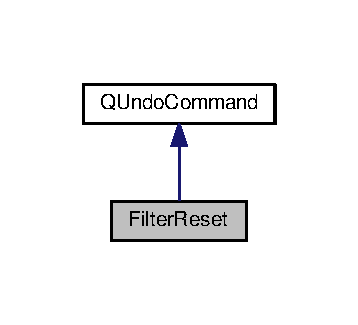
\includegraphics[width=172pt]{classUndoRedo_1_1FilterReset__inherit__graph}
\end{center}
\end{figure}
\subsection*{Public Member Functions}
\begin{DoxyCompactItemize}
\item 
\hyperlink{classUndoRedo_1_1FilterReset_ad3b8cc0805524eea48dae6eb1bddbdeb}{Filter\+Reset} (\hyperlink{classGUI_1_1FilterTab}{G\+U\+I\+::\+Filter\+Tab} $\ast$\hyperlink{classUndoRedo_1_1FilterReset_a47ca82534a740774d79998759818d9f4}{filter\+Tab}, \hyperlink{classModel_1_1FilterList}{Model\+::\+Filter\+List} \hyperlink{classUndoRedo_1_1FilterReset_ae1c4986a96d35566c0c7ebce2eeada53}{filter\+List})
\item 
void \hyperlink{classUndoRedo_1_1FilterReset_a0e1e7804a53f6d62efc72c9bdbec8571}{undo} ()
\item 
void \hyperlink{classUndoRedo_1_1FilterReset_a93c48d6ed036e1a381be53ac67643284}{redo} ()
\end{DoxyCompactItemize}
\subsection*{Private Attributes}
\begin{DoxyCompactItemize}
\item 
\hyperlink{classGUI_1_1FilterTab}{G\+U\+I\+::\+Filter\+Tab} $\ast$ \hyperlink{classUndoRedo_1_1FilterReset_a47ca82534a740774d79998759818d9f4}{filter\+Tab}
\item 
\hyperlink{classModel_1_1FilterList}{Model\+::\+Filter\+List} $\ast$ \hyperlink{classUndoRedo_1_1FilterReset_ae1c4986a96d35566c0c7ebce2eeada53}{filter\+List}
\end{DoxyCompactItemize}


\subsection{Detailed Description}
This class is the undo command for resting the filterlist in the filter tab. 

\subsection{Constructor \& Destructor Documentation}
\hypertarget{classUndoRedo_1_1FilterReset_ad3b8cc0805524eea48dae6eb1bddbdeb}{}\index{Undo\+Redo\+::\+Filter\+Reset@{Undo\+Redo\+::\+Filter\+Reset}!Filter\+Reset@{Filter\+Reset}}
\index{Filter\+Reset@{Filter\+Reset}!Undo\+Redo\+::\+Filter\+Reset@{Undo\+Redo\+::\+Filter\+Reset}}
\subsubsection[{Filter\+Reset}]{\setlength{\rightskip}{0pt plus 5cm}{\bf Filter\+Reset} (
\begin{DoxyParamCaption}
\item[{{\bf G\+U\+I\+::\+Filter\+Tab} $\ast$}]{filter\+Tab, }
\item[{{\bf Model\+::\+Filter\+List}}]{filter\+List}
\end{DoxyParamCaption}
)}\label{classUndoRedo_1_1FilterReset_ad3b8cc0805524eea48dae6eb1bddbdeb}


Constructor. 


\begin{DoxyParams}{Parameters}
{\em filter\+Tab} & The filtertab to operate on.\\
\hline
{\em filter\+List} & The filterlist the action to perform on.\\
\hline
\end{DoxyParams}


\subsection{Member Function Documentation}
\hypertarget{classUndoRedo_1_1FilterReset_a93c48d6ed036e1a381be53ac67643284}{}\index{Undo\+Redo\+::\+Filter\+Reset@{Undo\+Redo\+::\+Filter\+Reset}!redo@{redo}}
\index{redo@{redo}!Undo\+Redo\+::\+Filter\+Reset@{Undo\+Redo\+::\+Filter\+Reset}}
\subsubsection[{redo}]{\setlength{\rightskip}{0pt plus 5cm}void redo (
\begin{DoxyParamCaption}
{}
\end{DoxyParamCaption}
)}\label{classUndoRedo_1_1FilterReset_a93c48d6ed036e1a381be53ac67643284}


Clears the filter configurations and the filter list. 

\hypertarget{classUndoRedo_1_1FilterReset_a0e1e7804a53f6d62efc72c9bdbec8571}{}\index{Undo\+Redo\+::\+Filter\+Reset@{Undo\+Redo\+::\+Filter\+Reset}!undo@{undo}}
\index{undo@{undo}!Undo\+Redo\+::\+Filter\+Reset@{Undo\+Redo\+::\+Filter\+Reset}}
\subsubsection[{undo}]{\setlength{\rightskip}{0pt plus 5cm}void undo (
\begin{DoxyParamCaption}
{}
\end{DoxyParamCaption}
)}\label{classUndoRedo_1_1FilterReset_a0e1e7804a53f6d62efc72c9bdbec8571}


Loads the filterlist and filter configuration to the state it was before the reset. 



\subsection{Field Documentation}
\hypertarget{classUndoRedo_1_1FilterReset_ae1c4986a96d35566c0c7ebce2eeada53}{}\index{Undo\+Redo\+::\+Filter\+Reset@{Undo\+Redo\+::\+Filter\+Reset}!filter\+List@{filter\+List}}
\index{filter\+List@{filter\+List}!Undo\+Redo\+::\+Filter\+Reset@{Undo\+Redo\+::\+Filter\+Reset}}
\subsubsection[{filter\+List}]{\setlength{\rightskip}{0pt plus 5cm}{\bf Model\+::\+Filter\+List}$\ast$ filter\+List\hspace{0.3cm}{\ttfamily [private]}}\label{classUndoRedo_1_1FilterReset_ae1c4986a96d35566c0c7ebce2eeada53}
\hypertarget{classUndoRedo_1_1FilterReset_a47ca82534a740774d79998759818d9f4}{}\index{Undo\+Redo\+::\+Filter\+Reset@{Undo\+Redo\+::\+Filter\+Reset}!filter\+Tab@{filter\+Tab}}
\index{filter\+Tab@{filter\+Tab}!Undo\+Redo\+::\+Filter\+Reset@{Undo\+Redo\+::\+Filter\+Reset}}
\subsubsection[{filter\+Tab}]{\setlength{\rightskip}{0pt plus 5cm}{\bf G\+U\+I\+::\+Filter\+Tab}$\ast$ filter\+Tab\hspace{0.3cm}{\ttfamily [private]}}\label{classUndoRedo_1_1FilterReset_a47ca82534a740774d79998759818d9f4}

\newpage\hypertarget{classGUI_1_1FilterTab}{}\section{Filter\+Tab Class Reference}
\label{classGUI_1_1FilterTab}\index{Filter\+Tab@{Filter\+Tab}}
\subsection*{Public Member Functions}
\begin{DoxyCompactItemize}
\item 
\hyperlink{classGUI_1_1FilterTab_a3b29125d6d490f2cbdd22e453f79f6f9}{Filter\+Tab} (\hyperlink{classGUI_1_1QWidget}{G\+U\+I\+::\+Q\+Widget} $\ast$parent)
\item 
\hyperlink{classMemento_1_1FilterTabMemento}{Memento\+::\+Filter\+Tab\+Memento} \hyperlink{classGUI_1_1FilterTab_a7fc8423cb1fbba94b4f339ce1695312b}{get\+Memento} ()
\item 
void \hyperlink{classGUI_1_1FilterTab_a5ac565cc700848f69b7b30b83f9b7269}{restore} (\hyperlink{classMemento_1_1FilterTabMemento}{Memento\+::\+Filter\+Tab\+Memento} memento)
\item 
void \hyperlink{classGUI_1_1FilterTab_a3f8590a73c5ed6fd39daaa995e4fe04b}{insert\+Filter} (\hyperlink{classModel_1_1Filter}{Model\+::\+Filter} filter, int index=-\/1)
\item 
void \hyperlink{classGUI_1_1FilterTab_afbcb1308b246ae3f3008dd9854e1b276}{remove\+Filter} (string filter\+Name)
\item 
void \hyperlink{classGUI_1_1FilterTab_a8183c3773c11241bede44cedb223555f}{show\+Video} ()
\item 
void \hyperlink{classGUI_1_1FilterTab_a683e97e8ce40844fdccefc091a0e678e}{show\+Preview} ()
\item 
void \hyperlink{classGUI_1_1FilterTab_a4e238a9564770214fb84f0d542e846dc}{reset\+Filters} ()
\item 
void \hyperlink{classGUI_1_1FilterTab_a217572cdf98a98bd908c87600af7eb50}{set\+Filter\+List} (\hyperlink{classModel_1_1FilterList}{Model\+::\+Filter\+List} list)
\item 
void \hyperlink{classGUI_1_1FilterTab_ae01a11c0a081e873c992ebb245295903}{set\+Raw\+Video} (\hyperlink{classModel_1_1YuvVideo}{Model\+::\+Yuv\+Video} video)
\item 
void \hyperlink{classGUI_1_1FilterTab_a97ba0aa0c950aa895489093bbc6264f6}{move\+Filter} (int old, int new\+\_\+3)
\end{DoxyCompactItemize}
\subsection*{Data Fields}
\begin{DoxyCompactItemize}
\item 
\hyperlink{classUndoRedo_1_1LoadFilterVideo}{Undo\+Redo\+::\+Load\+Filter\+Video} $\ast$ \hyperlink{classGUI_1_1FilterTab_a2cf35b3ca5c4cf4888621bb7b2e103a7}{filter\+Tab}
\end{DoxyCompactItemize}
\subsection*{Private Member Functions}
\begin{DoxyCompactItemize}
\item 
void \hyperlink{classGUI_1_1FilterTab_ac3ca31ff0047daecf8bbe393a15e940c}{connect\+Actions} ()
\item 
void \hyperlink{classGUI_1_1FilterTab_aa72182c9a958af0e87b65ab7bdba0035}{create\+Ui} ()
\item 
void \hyperlink{classGUI_1_1FilterTab_a0a1d932d49dd1079cfd0964b11adc7a0}{up} ()
\item 
void \hyperlink{classGUI_1_1FilterTab_a6663cf1e20c2f8162d29d31c8f6324e6}{down} ()
\item 
void \hyperlink{classGUI_1_1FilterTab_a1fcb45e5d2428352eb36b487d1d4eea3}{remove} ()
\item 
void \hyperlink{classGUI_1_1FilterTab_a78f61ac2dd03bcba8e09ca20cd7d68e3}{load} ()
\item 
void \hyperlink{classGUI_1_1FilterTab_a95067243b72a23863ec07c821797455c}{apply} ()
\item 
void \hyperlink{classGUI_1_1FilterTab_aca3e1f51d9d95bb5f353275bda471260}{save\+Conf} ()
\item 
void \hyperlink{classGUI_1_1FilterTab_a6a47b95b078bb5310cd420104f09966f}{load\+Conf} ()
\item 
void \hyperlink{classGUI_1_1FilterTab_ad20897c5c8bd47f5d4005989bead0e55}{reset} ()
\item 
void \hyperlink{classGUI_1_1FilterTab_aae2c382151ef7c9aa913361172b30db6}{save} ()
\item 
void \hyperlink{classGUI_1_1FilterTab_a925c74d61941e57111324aa0d1f4bb85}{list\+Selection\+Changed} (Q\+Model\+Index index)
\end{DoxyCompactItemize}
\subsection*{Private Attributes}
\begin{DoxyCompactItemize}
\item 
Q\+Push\+Button $\ast$ \hyperlink{classGUI_1_1FilterTab_a7ffd636d50e89af94659d9b95f030d3a}{button\+\_\+up}
\item 
Q\+Push\+Button $\ast$ \hyperlink{classGUI_1_1FilterTab_ad858f8cd5d215c28f0f02f34d72cc2de}{button\+\_\+down}
\item 
Q\+Push\+Button $\ast$ \hyperlink{classGUI_1_1FilterTab_a3c9944c21208e29473ffc2a6d313fa84}{button\+\_\+remove}
\item 
Q\+Push\+Button $\ast$ \hyperlink{classGUI_1_1FilterTab_a73290dd82cac023039a9639ed4ee2a64}{button\+\_\+load}
\item 
Q\+Push\+Button $\ast$ \hyperlink{classGUI_1_1FilterTab_a41a7e158eeecc2ce4701674b848fb4ea}{button\+\_\+apply}
\item 
Q\+Push\+Button $\ast$ \hyperlink{classGUI_1_1FilterTab_a7c8a66ac3e3d168efff03a6da9a1ee02}{button\+\_\+save\+Conf}
\item 
Q\+Push\+Button $\ast$ \hyperlink{classGUI_1_1FilterTab_a83339040ed5dffc4a0f5b99b2a1ecf85}{button\+\_\+load\+Conf}
\item 
Q\+Push\+Button $\ast$ \hyperlink{classGUI_1_1FilterTab_a8ade1f6413d2829fcebef87d52e39904}{button\+\_\+reset}
\item 
Q\+Push\+Button $\ast$ \hyperlink{classGUI_1_1FilterTab_ac65ab223be901b07d3fb4ae0acf5f80f}{button\+\_\+save}
\item 
Q\+List\+Widget $\ast$ \hyperlink{classGUI_1_1FilterTab_a5fb61cc6e0821460452c387dab51bba3}{list\+\_\+filter\+List}
\item 
Q\+Tab\+Widget $\ast$ \hyperlink{classGUI_1_1FilterTab_ad0f0964c2d2113a68b9c59f4138e22e3}{tab\+\_\+filter\+Tabs}
\item 
Q\+Label $\ast$ \hyperlink{classGUI_1_1FilterTab_a6e618ac48cc8cd27bb7bbb1ae068dbcf}{label\+\_\+filter\+Options}
\item 
\hyperlink{classGUI_1_1QFrame}{G\+U\+I\+::\+Q\+Frame} $\ast$ \hyperlink{classGUI_1_1FilterTab_a16f45e31aa3e66824942b76aa75b4630}{frame\+\_\+filter\+Container}
\item 
Q\+String\+List\+Model $\ast$ \hyperlink{classGUI_1_1FilterTab_ac7d0d391532c07cc6745e6ef766e6b58}{model\+\_\+list}
\item 
\hyperlink{classGUI_1_1VideoPlayer}{G\+U\+I\+::\+Video\+Player} $\ast$ \hyperlink{classGUI_1_1FilterTab_a649e16c560960a5b48ca2ec6bc1a7232}{player}
\item 
\hyperlink{classGUI_1_1PreviewControlPanel}{G\+U\+I\+::\+Preview\+Control\+Panel} $\ast$ \hyperlink{classGUI_1_1FilterTab_a7ee97b60ba5c365fa8a4cdd3ab26bdb9}{preview\+Panel}
\item 
\hyperlink{classGUI_1_1FrameView}{G\+U\+I\+::\+Frame\+View} $\ast$ \hyperlink{classGUI_1_1FilterTab_a3fb59b508ebe75c20afa2e9e0fc3d862}{frame\+View}
\item 
\hyperlink{classGUI_1_1PlayerControlPanel}{G\+U\+I\+::\+Player\+Control\+Panel} $\ast$ \hyperlink{classGUI_1_1FilterTab_a20f9043c5269fd3d365cf6a6821d616d}{player\+Panel}
\item 
\hyperlink{classModel_1_1FilterList}{Model\+::\+Filter\+List} $\ast$ \hyperlink{classGUI_1_1FilterTab_ae1c4986a96d35566c0c7ebce2eeada53}{filter\+List}
\item 
\hyperlink{classModel_1_1YuvVideo}{Model\+::\+Yuv\+Video} $\ast$ \hyperlink{classGUI_1_1FilterTab_a095285c6e168db68548acccc569736ed}{raw\+Video}
\item 
std\+::vector$<$ \hyperlink{classGUI_1_1FilterContainerTab}{G\+U\+I\+::\+Filter\+Container\+Tab} $\ast$ $>$ \hyperlink{classGUI_1_1FilterTab_a3bfe5331038803533b637314ecf3351b}{filter\+Container\+Tab}
\end{DoxyCompactItemize}


\subsection{Detailed Description}
This class is the tab to filter videos. 

\subsection{Constructor \& Destructor Documentation}
\hypertarget{classGUI_1_1FilterTab_a3b29125d6d490f2cbdd22e453f79f6f9}{}\index{G\+U\+I\+::\+Filter\+Tab@{G\+U\+I\+::\+Filter\+Tab}!Filter\+Tab@{Filter\+Tab}}
\index{Filter\+Tab@{Filter\+Tab}!G\+U\+I\+::\+Filter\+Tab@{G\+U\+I\+::\+Filter\+Tab}}
\subsubsection[{Filter\+Tab}]{\setlength{\rightskip}{0pt plus 5cm}{\bf Filter\+Tab} (
\begin{DoxyParamCaption}
\item[{{\bf G\+U\+I\+::\+Q\+Widget} $\ast$}]{parent}
\end{DoxyParamCaption}
)}\label{classGUI_1_1FilterTab_a3b29125d6d490f2cbdd22e453f79f6f9}


Constructor. 



\subsection{Member Function Documentation}
\hypertarget{classGUI_1_1FilterTab_a95067243b72a23863ec07c821797455c}{}\index{G\+U\+I\+::\+Filter\+Tab@{G\+U\+I\+::\+Filter\+Tab}!apply@{apply}}
\index{apply@{apply}!G\+U\+I\+::\+Filter\+Tab@{G\+U\+I\+::\+Filter\+Tab}}
\subsubsection[{apply}]{\setlength{\rightskip}{0pt plus 5cm}void apply (
\begin{DoxyParamCaption}
{}
\end{DoxyParamCaption}
)\hspace{0.3cm}{\ttfamily [private]}}\label{classGUI_1_1FilterTab_a95067243b72a23863ec07c821797455c}


Slot\+: connected with button\+\_\+apply.\+pressed() applies the filter list on the video and shows it 

\hypertarget{classGUI_1_1FilterTab_ac3ca31ff0047daecf8bbe393a15e940c}{}\index{G\+U\+I\+::\+Filter\+Tab@{G\+U\+I\+::\+Filter\+Tab}!connect\+Actions@{connect\+Actions}}
\index{connect\+Actions@{connect\+Actions}!G\+U\+I\+::\+Filter\+Tab@{G\+U\+I\+::\+Filter\+Tab}}
\subsubsection[{connect\+Actions}]{\setlength{\rightskip}{0pt plus 5cm}void connect\+Actions (
\begin{DoxyParamCaption}
{}
\end{DoxyParamCaption}
)\hspace{0.3cm}{\ttfamily [private]}}\label{classGUI_1_1FilterTab_ac3ca31ff0047daecf8bbe393a15e940c}


Connect the buttons to their slots in this class. 

\hypertarget{classGUI_1_1FilterTab_aa72182c9a958af0e87b65ab7bdba0035}{}\index{G\+U\+I\+::\+Filter\+Tab@{G\+U\+I\+::\+Filter\+Tab}!create\+Ui@{create\+Ui}}
\index{create\+Ui@{create\+Ui}!G\+U\+I\+::\+Filter\+Tab@{G\+U\+I\+::\+Filter\+Tab}}
\subsubsection[{create\+Ui}]{\setlength{\rightskip}{0pt plus 5cm}void create\+Ui (
\begin{DoxyParamCaption}
{}
\end{DoxyParamCaption}
)\hspace{0.3cm}{\ttfamily [private]}}\label{classGUI_1_1FilterTab_aa72182c9a958af0e87b65ab7bdba0035}


Creates the user interface. 

\hypertarget{classGUI_1_1FilterTab_a6663cf1e20c2f8162d29d31c8f6324e6}{}\index{G\+U\+I\+::\+Filter\+Tab@{G\+U\+I\+::\+Filter\+Tab}!down@{down}}
\index{down@{down}!G\+U\+I\+::\+Filter\+Tab@{G\+U\+I\+::\+Filter\+Tab}}
\subsubsection[{down}]{\setlength{\rightskip}{0pt plus 5cm}void down (
\begin{DoxyParamCaption}
{}
\end{DoxyParamCaption}
)\hspace{0.3cm}{\ttfamily [private]}}\label{classGUI_1_1FilterTab_a6663cf1e20c2f8162d29d31c8f6324e6}


Slot\+: connected with button\+\_\+down.\+pressed() increases the index of a filter in the list 

\hypertarget{classGUI_1_1FilterTab_a7fc8423cb1fbba94b4f339ce1695312b}{}\index{G\+U\+I\+::\+Filter\+Tab@{G\+U\+I\+::\+Filter\+Tab}!get\+Memento@{get\+Memento}}
\index{get\+Memento@{get\+Memento}!G\+U\+I\+::\+Filter\+Tab@{G\+U\+I\+::\+Filter\+Tab}}
\subsubsection[{get\+Memento}]{\setlength{\rightskip}{0pt plus 5cm}{\bf Memento\+::\+Filter\+Tab\+Memento} get\+Memento (
\begin{DoxyParamCaption}
{}
\end{DoxyParamCaption}
)}\label{classGUI_1_1FilterTab_a7fc8423cb1fbba94b4f339ce1695312b}


Creates a memento which contains the state of this tab. 

\begin{DoxyReturn}{Returns}
The created memento.
\end{DoxyReturn}
\hypertarget{classGUI_1_1FilterTab_a3f8590a73c5ed6fd39daaa995e4fe04b}{}\index{G\+U\+I\+::\+Filter\+Tab@{G\+U\+I\+::\+Filter\+Tab}!insert\+Filter@{insert\+Filter}}
\index{insert\+Filter@{insert\+Filter}!G\+U\+I\+::\+Filter\+Tab@{G\+U\+I\+::\+Filter\+Tab}}
\subsubsection[{insert\+Filter}]{\setlength{\rightskip}{0pt plus 5cm}void insert\+Filter (
\begin{DoxyParamCaption}
\item[{{\bf Model\+::\+Filter}}]{filter, }
\item[{int}]{index = {\ttfamily -\/1}}
\end{DoxyParamCaption}
)}\label{classGUI_1_1FilterTab_a3f8590a73c5ed6fd39daaa995e4fe04b}


Inserts a filter to the filter\+List. If index is -\/1 the the filter is added to the end. 


\begin{DoxyParams}{Parameters}
{\em filter} & The filter to add.\\
\hline
{\em index} & The index to insert the filter at.\\
\hline
\end{DoxyParams}
\hypertarget{classGUI_1_1FilterTab_a925c74d61941e57111324aa0d1f4bb85}{}\index{G\+U\+I\+::\+Filter\+Tab@{G\+U\+I\+::\+Filter\+Tab}!list\+Selection\+Changed@{list\+Selection\+Changed}}
\index{list\+Selection\+Changed@{list\+Selection\+Changed}!G\+U\+I\+::\+Filter\+Tab@{G\+U\+I\+::\+Filter\+Tab}}
\subsubsection[{list\+Selection\+Changed}]{\setlength{\rightskip}{0pt plus 5cm}void list\+Selection\+Changed (
\begin{DoxyParamCaption}
\item[{Q\+Model\+Index}]{index}
\end{DoxyParamCaption}
)\hspace{0.3cm}{\ttfamily [private]}}\label{classGUI_1_1FilterTab_a925c74d61941e57111324aa0d1f4bb85}


Slot\+: connected with list\+\_\+filter\+List.\+clicked(index \+: Q\+Model\+Index); updates the filter\+Configuration\+Box that is shown 


\begin{DoxyParams}{Parameters}
{\em index} & Index of the selected item.\\
\hline
\end{DoxyParams}
\hypertarget{classGUI_1_1FilterTab_a78f61ac2dd03bcba8e09ca20cd7d68e3}{}\index{G\+U\+I\+::\+Filter\+Tab@{G\+U\+I\+::\+Filter\+Tab}!load@{load}}
\index{load@{load}!G\+U\+I\+::\+Filter\+Tab@{G\+U\+I\+::\+Filter\+Tab}}
\subsubsection[{load}]{\setlength{\rightskip}{0pt plus 5cm}void load (
\begin{DoxyParamCaption}
{}
\end{DoxyParamCaption}
)\hspace{0.3cm}{\ttfamily [private]}}\label{classGUI_1_1FilterTab_a78f61ac2dd03bcba8e09ca20cd7d68e3}


Slot\+: connected with button\+\_\+load.\+pressed() opens Q\+File\+Dialog and opens the video in the selected path 

\hypertarget{classGUI_1_1FilterTab_a6a47b95b078bb5310cd420104f09966f}{}\index{G\+U\+I\+::\+Filter\+Tab@{G\+U\+I\+::\+Filter\+Tab}!load\+Conf@{load\+Conf}}
\index{load\+Conf@{load\+Conf}!G\+U\+I\+::\+Filter\+Tab@{G\+U\+I\+::\+Filter\+Tab}}
\subsubsection[{load\+Conf}]{\setlength{\rightskip}{0pt plus 5cm}void load\+Conf (
\begin{DoxyParamCaption}
{}
\end{DoxyParamCaption}
)\hspace{0.3cm}{\ttfamily [private]}}\label{classGUI_1_1FilterTab_a6a47b95b078bb5310cd420104f09966f}


Slot\+: connected with button\+\_\+load\+Conf.\+pressed() opens Q\+File\+Dialog and loads the filter configuration in the selected path 

\hypertarget{classGUI_1_1FilterTab_a97ba0aa0c950aa895489093bbc6264f6}{}\index{G\+U\+I\+::\+Filter\+Tab@{G\+U\+I\+::\+Filter\+Tab}!move\+Filter@{move\+Filter}}
\index{move\+Filter@{move\+Filter}!G\+U\+I\+::\+Filter\+Tab@{G\+U\+I\+::\+Filter\+Tab}}
\subsubsection[{move\+Filter}]{\setlength{\rightskip}{0pt plus 5cm}void move\+Filter (
\begin{DoxyParamCaption}
\item[{int}]{old, }
\item[{int}]{new\+\_\+3}
\end{DoxyParamCaption}
)}\label{classGUI_1_1FilterTab_a97ba0aa0c950aa895489093bbc6264f6}


Moves a filter in the filterlist. 


\begin{DoxyParams}{Parameters}
{\em old} & Old list index.\\
\hline
{\em new} & New list index.\\
\hline
\end{DoxyParams}
\hypertarget{classGUI_1_1FilterTab_a1fcb45e5d2428352eb36b487d1d4eea3}{}\index{G\+U\+I\+::\+Filter\+Tab@{G\+U\+I\+::\+Filter\+Tab}!remove@{remove}}
\index{remove@{remove}!G\+U\+I\+::\+Filter\+Tab@{G\+U\+I\+::\+Filter\+Tab}}
\subsubsection[{remove}]{\setlength{\rightskip}{0pt plus 5cm}void remove (
\begin{DoxyParamCaption}
{}
\end{DoxyParamCaption}
)\hspace{0.3cm}{\ttfamily [private]}}\label{classGUI_1_1FilterTab_a1fcb45e5d2428352eb36b487d1d4eea3}


Slot\+: connected with button\+\_\+remove.\+pressed() removes a filter from the list 

\hypertarget{classGUI_1_1FilterTab_afbcb1308b246ae3f3008dd9854e1b276}{}\index{G\+U\+I\+::\+Filter\+Tab@{G\+U\+I\+::\+Filter\+Tab}!remove\+Filter@{remove\+Filter}}
\index{remove\+Filter@{remove\+Filter}!G\+U\+I\+::\+Filter\+Tab@{G\+U\+I\+::\+Filter\+Tab}}
\subsubsection[{remove\+Filter}]{\setlength{\rightskip}{0pt plus 5cm}void remove\+Filter (
\begin{DoxyParamCaption}
\item[{string}]{filter\+Name}
\end{DoxyParamCaption}
)}\label{classGUI_1_1FilterTab_afbcb1308b246ae3f3008dd9854e1b276}


Removes the filter with the name filter\+Name in the filterlist. 


\begin{DoxyParams}{Parameters}
{\em filter\+Name} & Name of the filter to remove.\\
\hline
\end{DoxyParams}
\hypertarget{classGUI_1_1FilterTab_ad20897c5c8bd47f5d4005989bead0e55}{}\index{G\+U\+I\+::\+Filter\+Tab@{G\+U\+I\+::\+Filter\+Tab}!reset@{reset}}
\index{reset@{reset}!G\+U\+I\+::\+Filter\+Tab@{G\+U\+I\+::\+Filter\+Tab}}
\subsubsection[{reset}]{\setlength{\rightskip}{0pt plus 5cm}void reset (
\begin{DoxyParamCaption}
{}
\end{DoxyParamCaption}
)\hspace{0.3cm}{\ttfamily [private]}}\label{classGUI_1_1FilterTab_ad20897c5c8bd47f5d4005989bead0e55}


Slot\+: connected with button\+\_\+reset.\+pressed() resets the filter list 

\hypertarget{classGUI_1_1FilterTab_a4e238a9564770214fb84f0d542e846dc}{}\index{G\+U\+I\+::\+Filter\+Tab@{G\+U\+I\+::\+Filter\+Tab}!reset\+Filters@{reset\+Filters}}
\index{reset\+Filters@{reset\+Filters}!G\+U\+I\+::\+Filter\+Tab@{G\+U\+I\+::\+Filter\+Tab}}
\subsubsection[{reset\+Filters}]{\setlength{\rightskip}{0pt plus 5cm}void reset\+Filters (
\begin{DoxyParamCaption}
{}
\end{DoxyParamCaption}
)}\label{classGUI_1_1FilterTab_a4e238a9564770214fb84f0d542e846dc}


Resets the filterlist. 

\hypertarget{classGUI_1_1FilterTab_a5ac565cc700848f69b7b30b83f9b7269}{}\index{G\+U\+I\+::\+Filter\+Tab@{G\+U\+I\+::\+Filter\+Tab}!restore@{restore}}
\index{restore@{restore}!G\+U\+I\+::\+Filter\+Tab@{G\+U\+I\+::\+Filter\+Tab}}
\subsubsection[{restore}]{\setlength{\rightskip}{0pt plus 5cm}void restore (
\begin{DoxyParamCaption}
\item[{{\bf Memento\+::\+Filter\+Tab\+Memento}}]{memento}
\end{DoxyParamCaption}
)}\label{classGUI_1_1FilterTab_a5ac565cc700848f69b7b30b83f9b7269}


Restores the tab based on the memento. 


\begin{DoxyParams}{Parameters}
{\em memento} & The memento which contains the state of the tab.\\
\hline
\end{DoxyParams}
\hypertarget{classGUI_1_1FilterTab_aae2c382151ef7c9aa913361172b30db6}{}\index{G\+U\+I\+::\+Filter\+Tab@{G\+U\+I\+::\+Filter\+Tab}!save@{save}}
\index{save@{save}!G\+U\+I\+::\+Filter\+Tab@{G\+U\+I\+::\+Filter\+Tab}}
\subsubsection[{save}]{\setlength{\rightskip}{0pt plus 5cm}void save (
\begin{DoxyParamCaption}
{}
\end{DoxyParamCaption}
)\hspace{0.3cm}{\ttfamily [private]}}\label{classGUI_1_1FilterTab_aae2c382151ef7c9aa913361172b30db6}


Slot\+: connected with button\+\_\+save.\+pressed() opens Q\+File\+Dialog and saves the video with the filters used on it. 

\hypertarget{classGUI_1_1FilterTab_aca3e1f51d9d95bb5f353275bda471260}{}\index{G\+U\+I\+::\+Filter\+Tab@{G\+U\+I\+::\+Filter\+Tab}!save\+Conf@{save\+Conf}}
\index{save\+Conf@{save\+Conf}!G\+U\+I\+::\+Filter\+Tab@{G\+U\+I\+::\+Filter\+Tab}}
\subsubsection[{save\+Conf}]{\setlength{\rightskip}{0pt plus 5cm}void save\+Conf (
\begin{DoxyParamCaption}
{}
\end{DoxyParamCaption}
)\hspace{0.3cm}{\ttfamily [private]}}\label{classGUI_1_1FilterTab_aca3e1f51d9d95bb5f353275bda471260}


Slot\+: connected with button\+\_\+save\+Conf.\+pressed() opens Q\+File\+Dialog and saves the filter configuration in the selected path 

\hypertarget{classGUI_1_1FilterTab_a217572cdf98a98bd908c87600af7eb50}{}\index{G\+U\+I\+::\+Filter\+Tab@{G\+U\+I\+::\+Filter\+Tab}!set\+Filter\+List@{set\+Filter\+List}}
\index{set\+Filter\+List@{set\+Filter\+List}!G\+U\+I\+::\+Filter\+Tab@{G\+U\+I\+::\+Filter\+Tab}}
\subsubsection[{set\+Filter\+List}]{\setlength{\rightskip}{0pt plus 5cm}void set\+Filter\+List (
\begin{DoxyParamCaption}
\item[{{\bf Model\+::\+Filter\+List}}]{list}
\end{DoxyParamCaption}
)}\label{classGUI_1_1FilterTab_a217572cdf98a98bd908c87600af7eb50}


Sets the filterlist. 


\begin{DoxyParams}{Parameters}
{\em list} & The filterlist to use.\\
\hline
\end{DoxyParams}
\hypertarget{classGUI_1_1FilterTab_ae01a11c0a081e873c992ebb245295903}{}\index{G\+U\+I\+::\+Filter\+Tab@{G\+U\+I\+::\+Filter\+Tab}!set\+Raw\+Video@{set\+Raw\+Video}}
\index{set\+Raw\+Video@{set\+Raw\+Video}!G\+U\+I\+::\+Filter\+Tab@{G\+U\+I\+::\+Filter\+Tab}}
\subsubsection[{set\+Raw\+Video}]{\setlength{\rightskip}{0pt plus 5cm}void set\+Raw\+Video (
\begin{DoxyParamCaption}
\item[{{\bf Model\+::\+Yuv\+Video}}]{video}
\end{DoxyParamCaption}
)}\label{classGUI_1_1FilterTab_ae01a11c0a081e873c992ebb245295903}


Sets the video the filters are applied to. This operation resets the whole filtertab. 


\begin{DoxyParams}{Parameters}
{\em video} & The video to apply the filters on.\\
\hline
\end{DoxyParams}
\hypertarget{classGUI_1_1FilterTab_a683e97e8ce40844fdccefc091a0e678e}{}\index{G\+U\+I\+::\+Filter\+Tab@{G\+U\+I\+::\+Filter\+Tab}!show\+Preview@{show\+Preview}}
\index{show\+Preview@{show\+Preview}!G\+U\+I\+::\+Filter\+Tab@{G\+U\+I\+::\+Filter\+Tab}}
\subsubsection[{show\+Preview}]{\setlength{\rightskip}{0pt plus 5cm}void show\+Preview (
\begin{DoxyParamCaption}
{}
\end{DoxyParamCaption}
)}\label{classGUI_1_1FilterTab_a683e97e8ce40844fdccefc091a0e678e}


Shows the 5 frame preview. 

\hypertarget{classGUI_1_1FilterTab_a8183c3773c11241bede44cedb223555f}{}\index{G\+U\+I\+::\+Filter\+Tab@{G\+U\+I\+::\+Filter\+Tab}!show\+Video@{show\+Video}}
\index{show\+Video@{show\+Video}!G\+U\+I\+::\+Filter\+Tab@{G\+U\+I\+::\+Filter\+Tab}}
\subsubsection[{show\+Video}]{\setlength{\rightskip}{0pt plus 5cm}void show\+Video (
\begin{DoxyParamCaption}
{}
\end{DoxyParamCaption}
)}\label{classGUI_1_1FilterTab_a8183c3773c11241bede44cedb223555f}


Shows the video with the applied filters. 

\hypertarget{classGUI_1_1FilterTab_a0a1d932d49dd1079cfd0964b11adc7a0}{}\index{G\+U\+I\+::\+Filter\+Tab@{G\+U\+I\+::\+Filter\+Tab}!up@{up}}
\index{up@{up}!G\+U\+I\+::\+Filter\+Tab@{G\+U\+I\+::\+Filter\+Tab}}
\subsubsection[{up}]{\setlength{\rightskip}{0pt plus 5cm}void up (
\begin{DoxyParamCaption}
{}
\end{DoxyParamCaption}
)\hspace{0.3cm}{\ttfamily [private]}}\label{classGUI_1_1FilterTab_a0a1d932d49dd1079cfd0964b11adc7a0}


Slot\+: connected with button\+\_\+up.\+pressed() decreases the index of a filter in the list 



\subsection{Field Documentation}
\hypertarget{classGUI_1_1FilterTab_a41a7e158eeecc2ce4701674b848fb4ea}{}\index{G\+U\+I\+::\+Filter\+Tab@{G\+U\+I\+::\+Filter\+Tab}!button\+\_\+apply@{button\+\_\+apply}}
\index{button\+\_\+apply@{button\+\_\+apply}!G\+U\+I\+::\+Filter\+Tab@{G\+U\+I\+::\+Filter\+Tab}}
\subsubsection[{button\+\_\+apply}]{\setlength{\rightskip}{0pt plus 5cm}Q\+Push\+Button$\ast$ button\+\_\+apply\hspace{0.3cm}{\ttfamily [private]}}\label{classGUI_1_1FilterTab_a41a7e158eeecc2ce4701674b848fb4ea}
\hypertarget{classGUI_1_1FilterTab_ad858f8cd5d215c28f0f02f34d72cc2de}{}\index{G\+U\+I\+::\+Filter\+Tab@{G\+U\+I\+::\+Filter\+Tab}!button\+\_\+down@{button\+\_\+down}}
\index{button\+\_\+down@{button\+\_\+down}!G\+U\+I\+::\+Filter\+Tab@{G\+U\+I\+::\+Filter\+Tab}}
\subsubsection[{button\+\_\+down}]{\setlength{\rightskip}{0pt plus 5cm}Q\+Push\+Button$\ast$ button\+\_\+down\hspace{0.3cm}{\ttfamily [private]}}\label{classGUI_1_1FilterTab_ad858f8cd5d215c28f0f02f34d72cc2de}
\hypertarget{classGUI_1_1FilterTab_a73290dd82cac023039a9639ed4ee2a64}{}\index{G\+U\+I\+::\+Filter\+Tab@{G\+U\+I\+::\+Filter\+Tab}!button\+\_\+load@{button\+\_\+load}}
\index{button\+\_\+load@{button\+\_\+load}!G\+U\+I\+::\+Filter\+Tab@{G\+U\+I\+::\+Filter\+Tab}}
\subsubsection[{button\+\_\+load}]{\setlength{\rightskip}{0pt plus 5cm}Q\+Push\+Button$\ast$ button\+\_\+load\hspace{0.3cm}{\ttfamily [private]}}\label{classGUI_1_1FilterTab_a73290dd82cac023039a9639ed4ee2a64}
\hypertarget{classGUI_1_1FilterTab_a83339040ed5dffc4a0f5b99b2a1ecf85}{}\index{G\+U\+I\+::\+Filter\+Tab@{G\+U\+I\+::\+Filter\+Tab}!button\+\_\+load\+Conf@{button\+\_\+load\+Conf}}
\index{button\+\_\+load\+Conf@{button\+\_\+load\+Conf}!G\+U\+I\+::\+Filter\+Tab@{G\+U\+I\+::\+Filter\+Tab}}
\subsubsection[{button\+\_\+load\+Conf}]{\setlength{\rightskip}{0pt plus 5cm}Q\+Push\+Button$\ast$ button\+\_\+load\+Conf\hspace{0.3cm}{\ttfamily [private]}}\label{classGUI_1_1FilterTab_a83339040ed5dffc4a0f5b99b2a1ecf85}
\hypertarget{classGUI_1_1FilterTab_a3c9944c21208e29473ffc2a6d313fa84}{}\index{G\+U\+I\+::\+Filter\+Tab@{G\+U\+I\+::\+Filter\+Tab}!button\+\_\+remove@{button\+\_\+remove}}
\index{button\+\_\+remove@{button\+\_\+remove}!G\+U\+I\+::\+Filter\+Tab@{G\+U\+I\+::\+Filter\+Tab}}
\subsubsection[{button\+\_\+remove}]{\setlength{\rightskip}{0pt plus 5cm}Q\+Push\+Button$\ast$ button\+\_\+remove\hspace{0.3cm}{\ttfamily [private]}}\label{classGUI_1_1FilterTab_a3c9944c21208e29473ffc2a6d313fa84}
\hypertarget{classGUI_1_1FilterTab_a8ade1f6413d2829fcebef87d52e39904}{}\index{G\+U\+I\+::\+Filter\+Tab@{G\+U\+I\+::\+Filter\+Tab}!button\+\_\+reset@{button\+\_\+reset}}
\index{button\+\_\+reset@{button\+\_\+reset}!G\+U\+I\+::\+Filter\+Tab@{G\+U\+I\+::\+Filter\+Tab}}
\subsubsection[{button\+\_\+reset}]{\setlength{\rightskip}{0pt plus 5cm}Q\+Push\+Button$\ast$ button\+\_\+reset\hspace{0.3cm}{\ttfamily [private]}}\label{classGUI_1_1FilterTab_a8ade1f6413d2829fcebef87d52e39904}
\hypertarget{classGUI_1_1FilterTab_ac65ab223be901b07d3fb4ae0acf5f80f}{}\index{G\+U\+I\+::\+Filter\+Tab@{G\+U\+I\+::\+Filter\+Tab}!button\+\_\+save@{button\+\_\+save}}
\index{button\+\_\+save@{button\+\_\+save}!G\+U\+I\+::\+Filter\+Tab@{G\+U\+I\+::\+Filter\+Tab}}
\subsubsection[{button\+\_\+save}]{\setlength{\rightskip}{0pt plus 5cm}Q\+Push\+Button$\ast$ button\+\_\+save\hspace{0.3cm}{\ttfamily [private]}}\label{classGUI_1_1FilterTab_ac65ab223be901b07d3fb4ae0acf5f80f}
\hypertarget{classGUI_1_1FilterTab_a7c8a66ac3e3d168efff03a6da9a1ee02}{}\index{G\+U\+I\+::\+Filter\+Tab@{G\+U\+I\+::\+Filter\+Tab}!button\+\_\+save\+Conf@{button\+\_\+save\+Conf}}
\index{button\+\_\+save\+Conf@{button\+\_\+save\+Conf}!G\+U\+I\+::\+Filter\+Tab@{G\+U\+I\+::\+Filter\+Tab}}
\subsubsection[{button\+\_\+save\+Conf}]{\setlength{\rightskip}{0pt plus 5cm}Q\+Push\+Button$\ast$ button\+\_\+save\+Conf\hspace{0.3cm}{\ttfamily [private]}}\label{classGUI_1_1FilterTab_a7c8a66ac3e3d168efff03a6da9a1ee02}
\hypertarget{classGUI_1_1FilterTab_a7ffd636d50e89af94659d9b95f030d3a}{}\index{G\+U\+I\+::\+Filter\+Tab@{G\+U\+I\+::\+Filter\+Tab}!button\+\_\+up@{button\+\_\+up}}
\index{button\+\_\+up@{button\+\_\+up}!G\+U\+I\+::\+Filter\+Tab@{G\+U\+I\+::\+Filter\+Tab}}
\subsubsection[{button\+\_\+up}]{\setlength{\rightskip}{0pt plus 5cm}Q\+Push\+Button$\ast$ button\+\_\+up\hspace{0.3cm}{\ttfamily [private]}}\label{classGUI_1_1FilterTab_a7ffd636d50e89af94659d9b95f030d3a}
\hypertarget{classGUI_1_1FilterTab_a3bfe5331038803533b637314ecf3351b}{}\index{G\+U\+I\+::\+Filter\+Tab@{G\+U\+I\+::\+Filter\+Tab}!filter\+Container\+Tab@{filter\+Container\+Tab}}
\index{filter\+Container\+Tab@{filter\+Container\+Tab}!G\+U\+I\+::\+Filter\+Tab@{G\+U\+I\+::\+Filter\+Tab}}
\subsubsection[{filter\+Container\+Tab}]{\setlength{\rightskip}{0pt plus 5cm}std\+::vector$<${\bf G\+U\+I\+::\+Filter\+Container\+Tab}$\ast$$>$ filter\+Container\+Tab\hspace{0.3cm}{\ttfamily [private]}}\label{classGUI_1_1FilterTab_a3bfe5331038803533b637314ecf3351b}
\hypertarget{classGUI_1_1FilterTab_ae1c4986a96d35566c0c7ebce2eeada53}{}\index{G\+U\+I\+::\+Filter\+Tab@{G\+U\+I\+::\+Filter\+Tab}!filter\+List@{filter\+List}}
\index{filter\+List@{filter\+List}!G\+U\+I\+::\+Filter\+Tab@{G\+U\+I\+::\+Filter\+Tab}}
\subsubsection[{filter\+List}]{\setlength{\rightskip}{0pt plus 5cm}{\bf Model\+::\+Filter\+List}$\ast$ filter\+List\hspace{0.3cm}{\ttfamily [private]}}\label{classGUI_1_1FilterTab_ae1c4986a96d35566c0c7ebce2eeada53}
\hypertarget{classGUI_1_1FilterTab_a2cf35b3ca5c4cf4888621bb7b2e103a7}{}\index{G\+U\+I\+::\+Filter\+Tab@{G\+U\+I\+::\+Filter\+Tab}!filter\+Tab@{filter\+Tab}}
\index{filter\+Tab@{filter\+Tab}!G\+U\+I\+::\+Filter\+Tab@{G\+U\+I\+::\+Filter\+Tab}}
\subsubsection[{filter\+Tab}]{\setlength{\rightskip}{0pt plus 5cm}{\bf Undo\+Redo\+::\+Load\+Filter\+Video}$\ast$ filter\+Tab}\label{classGUI_1_1FilterTab_a2cf35b3ca5c4cf4888621bb7b2e103a7}
\hypertarget{classGUI_1_1FilterTab_a16f45e31aa3e66824942b76aa75b4630}{}\index{G\+U\+I\+::\+Filter\+Tab@{G\+U\+I\+::\+Filter\+Tab}!frame\+\_\+filter\+Container@{frame\+\_\+filter\+Container}}
\index{frame\+\_\+filter\+Container@{frame\+\_\+filter\+Container}!G\+U\+I\+::\+Filter\+Tab@{G\+U\+I\+::\+Filter\+Tab}}
\subsubsection[{frame\+\_\+filter\+Container}]{\setlength{\rightskip}{0pt plus 5cm}{\bf G\+U\+I\+::\+Q\+Frame}$\ast$ frame\+\_\+filter\+Container\hspace{0.3cm}{\ttfamily [private]}}\label{classGUI_1_1FilterTab_a16f45e31aa3e66824942b76aa75b4630}
\hypertarget{classGUI_1_1FilterTab_a3fb59b508ebe75c20afa2e9e0fc3d862}{}\index{G\+U\+I\+::\+Filter\+Tab@{G\+U\+I\+::\+Filter\+Tab}!frame\+View@{frame\+View}}
\index{frame\+View@{frame\+View}!G\+U\+I\+::\+Filter\+Tab@{G\+U\+I\+::\+Filter\+Tab}}
\subsubsection[{frame\+View}]{\setlength{\rightskip}{0pt plus 5cm}{\bf G\+U\+I\+::\+Frame\+View}$\ast$ frame\+View\hspace{0.3cm}{\ttfamily [private]}}\label{classGUI_1_1FilterTab_a3fb59b508ebe75c20afa2e9e0fc3d862}
\hypertarget{classGUI_1_1FilterTab_a6e618ac48cc8cd27bb7bbb1ae068dbcf}{}\index{G\+U\+I\+::\+Filter\+Tab@{G\+U\+I\+::\+Filter\+Tab}!label\+\_\+filter\+Options@{label\+\_\+filter\+Options}}
\index{label\+\_\+filter\+Options@{label\+\_\+filter\+Options}!G\+U\+I\+::\+Filter\+Tab@{G\+U\+I\+::\+Filter\+Tab}}
\subsubsection[{label\+\_\+filter\+Options}]{\setlength{\rightskip}{0pt plus 5cm}Q\+Label$\ast$ label\+\_\+filter\+Options\hspace{0.3cm}{\ttfamily [private]}}\label{classGUI_1_1FilterTab_a6e618ac48cc8cd27bb7bbb1ae068dbcf}
\hypertarget{classGUI_1_1FilterTab_a5fb61cc6e0821460452c387dab51bba3}{}\index{G\+U\+I\+::\+Filter\+Tab@{G\+U\+I\+::\+Filter\+Tab}!list\+\_\+filter\+List@{list\+\_\+filter\+List}}
\index{list\+\_\+filter\+List@{list\+\_\+filter\+List}!G\+U\+I\+::\+Filter\+Tab@{G\+U\+I\+::\+Filter\+Tab}}
\subsubsection[{list\+\_\+filter\+List}]{\setlength{\rightskip}{0pt plus 5cm}Q\+List\+Widget$\ast$ list\+\_\+filter\+List\hspace{0.3cm}{\ttfamily [private]}}\label{classGUI_1_1FilterTab_a5fb61cc6e0821460452c387dab51bba3}
\hypertarget{classGUI_1_1FilterTab_ac7d0d391532c07cc6745e6ef766e6b58}{}\index{G\+U\+I\+::\+Filter\+Tab@{G\+U\+I\+::\+Filter\+Tab}!model\+\_\+list@{model\+\_\+list}}
\index{model\+\_\+list@{model\+\_\+list}!G\+U\+I\+::\+Filter\+Tab@{G\+U\+I\+::\+Filter\+Tab}}
\subsubsection[{model\+\_\+list}]{\setlength{\rightskip}{0pt plus 5cm}Q\+String\+List\+Model$\ast$ model\+\_\+list\hspace{0.3cm}{\ttfamily [private]}}\label{classGUI_1_1FilterTab_ac7d0d391532c07cc6745e6ef766e6b58}
\hypertarget{classGUI_1_1FilterTab_a649e16c560960a5b48ca2ec6bc1a7232}{}\index{G\+U\+I\+::\+Filter\+Tab@{G\+U\+I\+::\+Filter\+Tab}!player@{player}}
\index{player@{player}!G\+U\+I\+::\+Filter\+Tab@{G\+U\+I\+::\+Filter\+Tab}}
\subsubsection[{player}]{\setlength{\rightskip}{0pt plus 5cm}{\bf G\+U\+I\+::\+Video\+Player}$\ast$ player\hspace{0.3cm}{\ttfamily [private]}}\label{classGUI_1_1FilterTab_a649e16c560960a5b48ca2ec6bc1a7232}
\hypertarget{classGUI_1_1FilterTab_a20f9043c5269fd3d365cf6a6821d616d}{}\index{G\+U\+I\+::\+Filter\+Tab@{G\+U\+I\+::\+Filter\+Tab}!player\+Panel@{player\+Panel}}
\index{player\+Panel@{player\+Panel}!G\+U\+I\+::\+Filter\+Tab@{G\+U\+I\+::\+Filter\+Tab}}
\subsubsection[{player\+Panel}]{\setlength{\rightskip}{0pt plus 5cm}{\bf G\+U\+I\+::\+Player\+Control\+Panel}$\ast$ player\+Panel\hspace{0.3cm}{\ttfamily [private]}}\label{classGUI_1_1FilterTab_a20f9043c5269fd3d365cf6a6821d616d}
\hypertarget{classGUI_1_1FilterTab_a7ee97b60ba5c365fa8a4cdd3ab26bdb9}{}\index{G\+U\+I\+::\+Filter\+Tab@{G\+U\+I\+::\+Filter\+Tab}!preview\+Panel@{preview\+Panel}}
\index{preview\+Panel@{preview\+Panel}!G\+U\+I\+::\+Filter\+Tab@{G\+U\+I\+::\+Filter\+Tab}}
\subsubsection[{preview\+Panel}]{\setlength{\rightskip}{0pt plus 5cm}{\bf G\+U\+I\+::\+Preview\+Control\+Panel}$\ast$ preview\+Panel\hspace{0.3cm}{\ttfamily [private]}}\label{classGUI_1_1FilterTab_a7ee97b60ba5c365fa8a4cdd3ab26bdb9}
\hypertarget{classGUI_1_1FilterTab_a095285c6e168db68548acccc569736ed}{}\index{G\+U\+I\+::\+Filter\+Tab@{G\+U\+I\+::\+Filter\+Tab}!raw\+Video@{raw\+Video}}
\index{raw\+Video@{raw\+Video}!G\+U\+I\+::\+Filter\+Tab@{G\+U\+I\+::\+Filter\+Tab}}
\subsubsection[{raw\+Video}]{\setlength{\rightskip}{0pt plus 5cm}{\bf Model\+::\+Yuv\+Video}$\ast$ raw\+Video\hspace{0.3cm}{\ttfamily [private]}}\label{classGUI_1_1FilterTab_a095285c6e168db68548acccc569736ed}
\hypertarget{classGUI_1_1FilterTab_ad0f0964c2d2113a68b9c59f4138e22e3}{}\index{G\+U\+I\+::\+Filter\+Tab@{G\+U\+I\+::\+Filter\+Tab}!tab\+\_\+filter\+Tabs@{tab\+\_\+filter\+Tabs}}
\index{tab\+\_\+filter\+Tabs@{tab\+\_\+filter\+Tabs}!G\+U\+I\+::\+Filter\+Tab@{G\+U\+I\+::\+Filter\+Tab}}
\subsubsection[{tab\+\_\+filter\+Tabs}]{\setlength{\rightskip}{0pt plus 5cm}Q\+Tab\+Widget$\ast$ tab\+\_\+filter\+Tabs\hspace{0.3cm}{\ttfamily [private]}}\label{classGUI_1_1FilterTab_ad0f0964c2d2113a68b9c59f4138e22e3}

\newpage\hypertarget{classMemento_1_1FilterTabMemento}{}\section{Filter\+Tab\+Memento Class Reference}
\label{classMemento_1_1FilterTabMemento}\index{Filter\+Tab\+Memento@{Filter\+Tab\+Memento}}
\subsection*{Public Member Functions}
\begin{DoxyCompactItemize}
\item 
\hyperlink{classMemento_1_1FilterTabMemento_a84a5fcbb2f69b5b3c57dae3540fdd40b}{Filter\+Tab\+Memento} ()
\item 
\hyperlink{classModel_1_1Filter_1_1FilterList}{Model\+::\+Filter\+::\+Filter\+List} \hyperlink{classMemento_1_1FilterTabMemento_a8f68d1381e85b679f08fb6208565af24}{get\+Filter\+List} ()
\item 
void \hyperlink{classMemento_1_1FilterTabMemento_aa18e770b0715c18549678cb5241b8714}{set\+Filter\+List} (\hyperlink{classModel_1_1Filter_1_1FilterList}{Model\+::\+Filter\+::\+Filter\+List} filter\+List)
\item 
bool \hyperlink{classMemento_1_1FilterTabMemento_aece4e0d122e3afae0c4173edba6a4cc8}{get\+Was\+Applied} ()
\item 
void \hyperlink{classMemento_1_1FilterTabMemento_a635ac39ad3547885c6d8a5f631a86aeb}{set\+Was\+Applied} (bool was\+Applied)
\item 
int \hyperlink{classMemento_1_1FilterTabMemento_a116429d102ca02253915c78f76d305d2}{get\+Displayed\+Frame} ()
\item 
void \hyperlink{classMemento_1_1FilterTabMemento_ad3eeeb568c249bd940edc513b0697cd8}{set\+Displayed\+Frame} (int displayed\+Frame)
\item 
string \hyperlink{classMemento_1_1FilterTabMemento_aef6a8daef5ed9e5ac0862ef4323f3f8d}{get\+Loaded\+File} ()
\item 
void \hyperlink{classMemento_1_1FilterTabMemento_a2dc9fb31a997a0f4d76aa4b6d11c12c9}{set\+Loaded\+File} (string loaded\+File)
\end{DoxyCompactItemize}


\subsection{Detailed Description}
This class is the memento for the Filter\+Tab. 

\subsection{Constructor \& Destructor Documentation}
\hypertarget{classMemento_1_1FilterTabMemento_a84a5fcbb2f69b5b3c57dae3540fdd40b}{}\index{Memento\+::\+Filter\+Tab\+Memento@{Memento\+::\+Filter\+Tab\+Memento}!Filter\+Tab\+Memento@{Filter\+Tab\+Memento}}
\index{Filter\+Tab\+Memento@{Filter\+Tab\+Memento}!Memento\+::\+Filter\+Tab\+Memento@{Memento\+::\+Filter\+Tab\+Memento}}
\subsubsection[{Filter\+Tab\+Memento}]{\setlength{\rightskip}{0pt plus 5cm}{\bf Filter\+Tab\+Memento} (
\begin{DoxyParamCaption}
{}
\end{DoxyParamCaption}
)}\label{classMemento_1_1FilterTabMemento_a84a5fcbb2f69b5b3c57dae3540fdd40b}


Constructor. 



\subsection{Member Function Documentation}
\hypertarget{classMemento_1_1FilterTabMemento_a116429d102ca02253915c78f76d305d2}{}\index{Memento\+::\+Filter\+Tab\+Memento@{Memento\+::\+Filter\+Tab\+Memento}!get\+Displayed\+Frame@{get\+Displayed\+Frame}}
\index{get\+Displayed\+Frame@{get\+Displayed\+Frame}!Memento\+::\+Filter\+Tab\+Memento@{Memento\+::\+Filter\+Tab\+Memento}}
\subsubsection[{get\+Displayed\+Frame}]{\setlength{\rightskip}{0pt plus 5cm}int get\+Displayed\+Frame (
\begin{DoxyParamCaption}
{}
\end{DoxyParamCaption}
)}\label{classMemento_1_1FilterTabMemento_a116429d102ca02253915c78f76d305d2}


Returns the currently displayed frame in the frame preview. 

\begin{DoxyReturn}{Returns}
the currently displayed frame
\end{DoxyReturn}
\hypertarget{classMemento_1_1FilterTabMemento_a8f68d1381e85b679f08fb6208565af24}{}\index{Memento\+::\+Filter\+Tab\+Memento@{Memento\+::\+Filter\+Tab\+Memento}!get\+Filter\+List@{get\+Filter\+List}}
\index{get\+Filter\+List@{get\+Filter\+List}!Memento\+::\+Filter\+Tab\+Memento@{Memento\+::\+Filter\+Tab\+Memento}}
\subsubsection[{get\+Filter\+List}]{\setlength{\rightskip}{0pt plus 5cm}{\bf Model\+::\+Filter\+::\+Filter\+List} get\+Filter\+List (
\begin{DoxyParamCaption}
{}
\end{DoxyParamCaption}
)}\label{classMemento_1_1FilterTabMemento_a8f68d1381e85b679f08fb6208565af24}


Returns the list of the currently selected  filters. 

\begin{DoxyReturn}{Returns}
list of the selected filters
\end{DoxyReturn}
\hypertarget{classMemento_1_1FilterTabMemento_aef6a8daef5ed9e5ac0862ef4323f3f8d}{}\index{Memento\+::\+Filter\+Tab\+Memento@{Memento\+::\+Filter\+Tab\+Memento}!get\+Loaded\+File@{get\+Loaded\+File}}
\index{get\+Loaded\+File@{get\+Loaded\+File}!Memento\+::\+Filter\+Tab\+Memento@{Memento\+::\+Filter\+Tab\+Memento}}
\subsubsection[{get\+Loaded\+File}]{\setlength{\rightskip}{0pt plus 5cm}string get\+Loaded\+File (
\begin{DoxyParamCaption}
{}
\end{DoxyParamCaption}
)}\label{classMemento_1_1FilterTabMemento_aef6a8daef5ed9e5ac0862ef4323f3f8d}


Returns the path to the currently loaded yuv file. 

\begin{DoxyReturn}{Returns}
absolute path to the currently loaded yuv file
\end{DoxyReturn}
\hypertarget{classMemento_1_1FilterTabMemento_aece4e0d122e3afae0c4173edba6a4cc8}{}\index{Memento\+::\+Filter\+Tab\+Memento@{Memento\+::\+Filter\+Tab\+Memento}!get\+Was\+Applied@{get\+Was\+Applied}}
\index{get\+Was\+Applied@{get\+Was\+Applied}!Memento\+::\+Filter\+Tab\+Memento@{Memento\+::\+Filter\+Tab\+Memento}}
\subsubsection[{get\+Was\+Applied}]{\setlength{\rightskip}{0pt plus 5cm}bool get\+Was\+Applied (
\begin{DoxyParamCaption}
{}
\end{DoxyParamCaption}
)}\label{classMemento_1_1FilterTabMemento_aece4e0d122e3afae0c4173edba6a4cc8}


Whether the filter were already applied. 

\begin{DoxyReturn}{Returns}
true if the filter wre already applied
\end{DoxyReturn}
\hypertarget{classMemento_1_1FilterTabMemento_ad3eeeb568c249bd940edc513b0697cd8}{}\index{Memento\+::\+Filter\+Tab\+Memento@{Memento\+::\+Filter\+Tab\+Memento}!set\+Displayed\+Frame@{set\+Displayed\+Frame}}
\index{set\+Displayed\+Frame@{set\+Displayed\+Frame}!Memento\+::\+Filter\+Tab\+Memento@{Memento\+::\+Filter\+Tab\+Memento}}
\subsubsection[{set\+Displayed\+Frame}]{\setlength{\rightskip}{0pt plus 5cm}void set\+Displayed\+Frame (
\begin{DoxyParamCaption}
\item[{int}]{displayed\+Frame}
\end{DoxyParamCaption}
)}\label{classMemento_1_1FilterTabMemento_ad3eeeb568c249bd940edc513b0697cd8}


Sets the currently displayed frame in the frame preview. 


\begin{DoxyParams}{Parameters}
{\em displayed\+Frame} & the currently displayed frame\\
\hline
\end{DoxyParams}
\hypertarget{classMemento_1_1FilterTabMemento_aa18e770b0715c18549678cb5241b8714}{}\index{Memento\+::\+Filter\+Tab\+Memento@{Memento\+::\+Filter\+Tab\+Memento}!set\+Filter\+List@{set\+Filter\+List}}
\index{set\+Filter\+List@{set\+Filter\+List}!Memento\+::\+Filter\+Tab\+Memento@{Memento\+::\+Filter\+Tab\+Memento}}
\subsubsection[{set\+Filter\+List}]{\setlength{\rightskip}{0pt plus 5cm}void set\+Filter\+List (
\begin{DoxyParamCaption}
\item[{{\bf Model\+::\+Filter\+::\+Filter\+List}}]{filter\+List}
\end{DoxyParamCaption}
)}\label{classMemento_1_1FilterTabMemento_aa18e770b0715c18549678cb5241b8714}


Sets the list of the currently selected filters. 


\begin{DoxyParams}{Parameters}
{\em filter\+List} & list of the selected filters\\
\hline
\end{DoxyParams}
\hypertarget{classMemento_1_1FilterTabMemento_a2dc9fb31a997a0f4d76aa4b6d11c12c9}{}\index{Memento\+::\+Filter\+Tab\+Memento@{Memento\+::\+Filter\+Tab\+Memento}!set\+Loaded\+File@{set\+Loaded\+File}}
\index{set\+Loaded\+File@{set\+Loaded\+File}!Memento\+::\+Filter\+Tab\+Memento@{Memento\+::\+Filter\+Tab\+Memento}}
\subsubsection[{set\+Loaded\+File}]{\setlength{\rightskip}{0pt plus 5cm}void set\+Loaded\+File (
\begin{DoxyParamCaption}
\item[{string}]{loaded\+File}
\end{DoxyParamCaption}
)}\label{classMemento_1_1FilterTabMemento_a2dc9fb31a997a0f4d76aa4b6d11c12c9}


Sets the path to the currently loaded yuv file. 


\begin{DoxyParams}{Parameters}
{\em loaded\+File} & absolute path to the loaded yuv file\\
\hline
\end{DoxyParams}
\hypertarget{classMemento_1_1FilterTabMemento_a635ac39ad3547885c6d8a5f631a86aeb}{}\index{Memento\+::\+Filter\+Tab\+Memento@{Memento\+::\+Filter\+Tab\+Memento}!set\+Was\+Applied@{set\+Was\+Applied}}
\index{set\+Was\+Applied@{set\+Was\+Applied}!Memento\+::\+Filter\+Tab\+Memento@{Memento\+::\+Filter\+Tab\+Memento}}
\subsubsection[{set\+Was\+Applied}]{\setlength{\rightskip}{0pt plus 5cm}void set\+Was\+Applied (
\begin{DoxyParamCaption}
\item[{bool}]{was\+Applied}
\end{DoxyParamCaption}
)}\label{classMemento_1_1FilterTabMemento_a635ac39ad3547885c6d8a5f631a86aeb}


Sets whether the filters were already aplied. 


\begin{DoxyParams}{Parameters}
{\em was\+Applied} & true if the filter were already applied\\
\hline
\end{DoxyParams}

\newpage\hypertarget{classGUI_1_1FilterView}{}\section{Filter\+View Class Reference}
\label{classGUI_1_1FilterView}\index{Filter\+View@{Filter\+View}}
\subsection*{Public Member Functions}
\begin{DoxyCompactItemize}
\item 
\hypertarget{classGUI_1_1FilterView_aa31e034ecd1383cc8b2f35285f208764}{}{\bfseries Filter\+View} (\hyperlink{classGUI_1_1QtGui_1_1QWidget____10}{G\+U\+I\+::\+Qt\+Gui\+::\+Q\+Widget\+\_\+\+\_\+10} $\ast$parent)\label{classGUI_1_1FilterView_aa31e034ecd1383cc8b2f35285f208764}

\item 
\hypertarget{classGUI_1_1FilterView_a5b70d646670fa62496626d2a3248598c}{}void {\bfseries set\+Filter} (\hyperlink{classModel_1_1Filter_1_1Filter}{Model\+::\+Filter\+::\+Filter} filter)\label{classGUI_1_1FilterView_a5b70d646670fa62496626d2a3248598c}

\item 
\hypertarget{classGUI_1_1FilterView_a8732f98917f4cf76c86e9c4d6df1ce70}{}void {\bfseries set\+Filter\+Tab} (\hyperlink{classGUI_1_1FilterTab}{G\+U\+I\+::\+Filter\+Tab} $\ast$filtertab)\label{classGUI_1_1FilterView_a8732f98917f4cf76c86e9c4d6df1ce70}

\end{DoxyCompactItemize}


\subsection{Detailed Description}
represents a filter in the gui, shows a example of the filter and  a checkbox as well as its name 
\newpage\hypertarget{classGUI_1_1ForwardPlayer}{}\section{Forward\+Player Class Reference}
\label{classGUI_1_1ForwardPlayer}\index{Forward\+Player@{Forward\+Player}}
\subsection*{Public Member Functions}
\begin{DoxyCompactItemize}
\item 
\hyperlink{classGUI_1_1ForwardPlayer_a61bebb272dd2685ca2bfdf72349bc0f1}{Forward\+Player} ()
\item 
void \hyperlink{classGUI_1_1ForwardPlayer_a197c17c5b8dc04f8c311b41763a9db0e}{set\+Forward\+Control\+Panel} (\hyperlink{classGUI_1_1Player_1_1ControlPanel}{G\+U\+I\+::\+Player\+::\+Control\+Panel} panel)
\item 
void \hyperlink{classGUI_1_1ForwardPlayer_a6d58098c6cf63c241ed03bc797256bb1}{play} ()
\item 
void \hyperlink{classGUI_1_1ForwardPlayer_a7167f5c196fc5e167bfabde1a730e81d}{pause} ()
\item 
void \hyperlink{classGUI_1_1ForwardPlayer_a8c528baf37154d347366083f0f816846}{stop} ()
\item 
void \hyperlink{classGUI_1_1ForwardPlayer_a365329da56f8b07f8c95027ba967bbc3}{next\+Frame} ()
\item 
void \hyperlink{classGUI_1_1ForwardPlayer_a3c96ed37c70ebc0b32c527a04e1536d1}{previous\+Frame} ()
\item 
void \hyperlink{classGUI_1_1ForwardPlayer_a5466c67c5ec22359c0702dc4ac8ffb19}{set\+Speed} (float speed)
\item 
void \hyperlink{classGUI_1_1ForwardPlayer_a1aa68f77243229daea38d59bc5145d35}{set\+Position} (int position)
\item 
int \hyperlink{classGUI_1_1ForwardPlayer_a97825791568ee242ca19d25b75030d87}{get\+Position} ()
\item 
float \hyperlink{classGUI_1_1ForwardPlayer_a26ebefde7fe71954e6c1282255951b7d}{get\+Speed} ()
\item 
bool \hyperlink{classGUI_1_1ForwardPlayer_a8438e3403946accc1986a05b89ee7b03}{is\+Playing} ()
\item 
bool \hyperlink{classGUI_1_1ForwardPlayer_a2fc5ff4f369aaa46c55c3ad3c63216d6}{is\+Stopped} ()
\item 
void \hyperlink{classGUI_1_1ForwardPlayer_ad20897c5c8bd47f5d4005989bead0e55}{reset} ()
\end{DoxyCompactItemize}
\subsection*{Additional Inherited Members}


\subsection{Detailed Description}
This player forwards its input to a Control\+Panel. 

\subsection{Constructor \& Destructor Documentation}
\hypertarget{classGUI_1_1ForwardPlayer_a61bebb272dd2685ca2bfdf72349bc0f1}{}\index{G\+U\+I\+::\+Forward\+Player@{G\+U\+I\+::\+Forward\+Player}!Forward\+Player@{Forward\+Player}}
\index{Forward\+Player@{Forward\+Player}!G\+U\+I\+::\+Forward\+Player@{G\+U\+I\+::\+Forward\+Player}}
\subsubsection[{Forward\+Player}]{\setlength{\rightskip}{0pt plus 5cm}{\bf Forward\+Player} (
\begin{DoxyParamCaption}
{}
\end{DoxyParamCaption}
)}\label{classGUI_1_1ForwardPlayer_a61bebb272dd2685ca2bfdf72349bc0f1}


Constructor. 



\subsection{Member Function Documentation}
\hypertarget{classGUI_1_1ForwardPlayer_a97825791568ee242ca19d25b75030d87}{}\index{G\+U\+I\+::\+Forward\+Player@{G\+U\+I\+::\+Forward\+Player}!get\+Position@{get\+Position}}
\index{get\+Position@{get\+Position}!G\+U\+I\+::\+Forward\+Player@{G\+U\+I\+::\+Forward\+Player}}
\subsubsection[{get\+Position}]{\setlength{\rightskip}{0pt plus 5cm}int get\+Position (
\begin{DoxyParamCaption}
{}
\end{DoxyParamCaption}
)\hspace{0.3cm}{\ttfamily [virtual]}}\label{classGUI_1_1ForwardPlayer_a97825791568ee242ca19d25b75030d87}


Returns the position in the video. 

\begin{DoxyReturn}{Returns}
The current position.
\end{DoxyReturn}


Implements \hyperlink{classGUI_1_1Player_1_1Player_a889dbfa5524d69dcc31d377d2d9bd230}{Player}.

\hypertarget{classGUI_1_1ForwardPlayer_a26ebefde7fe71954e6c1282255951b7d}{}\index{G\+U\+I\+::\+Forward\+Player@{G\+U\+I\+::\+Forward\+Player}!get\+Speed@{get\+Speed}}
\index{get\+Speed@{get\+Speed}!G\+U\+I\+::\+Forward\+Player@{G\+U\+I\+::\+Forward\+Player}}
\subsubsection[{get\+Speed}]{\setlength{\rightskip}{0pt plus 5cm}float get\+Speed (
\begin{DoxyParamCaption}
{}
\end{DoxyParamCaption}
)\hspace{0.3cm}{\ttfamily [virtual]}}\label{classGUI_1_1ForwardPlayer_a26ebefde7fe71954e6c1282255951b7d}


Returns the speed. 

\begin{DoxyReturn}{Returns}
The current speed.
\end{DoxyReturn}


Implements \hyperlink{classGUI_1_1Player_1_1Player_a349fa93e666bd9fb256a238a3194f948}{Player}.

\hypertarget{classGUI_1_1ForwardPlayer_a8438e3403946accc1986a05b89ee7b03}{}\index{G\+U\+I\+::\+Forward\+Player@{G\+U\+I\+::\+Forward\+Player}!is\+Playing@{is\+Playing}}
\index{is\+Playing@{is\+Playing}!G\+U\+I\+::\+Forward\+Player@{G\+U\+I\+::\+Forward\+Player}}
\subsubsection[{is\+Playing}]{\setlength{\rightskip}{0pt plus 5cm}bool is\+Playing (
\begin{DoxyParamCaption}
{}
\end{DoxyParamCaption}
)\hspace{0.3cm}{\ttfamily [virtual]}}\label{classGUI_1_1ForwardPlayer_a8438e3403946accc1986a05b89ee7b03}


Whether the player is currently playing. 

\begin{DoxyReturn}{Returns}
True if the player is playing.
\end{DoxyReturn}


Implements \hyperlink{classGUI_1_1Player_1_1Player_a4fbad8972dd248e6c8f5dc2c898a9bc7}{Player}.

\hypertarget{classGUI_1_1ForwardPlayer_a2fc5ff4f369aaa46c55c3ad3c63216d6}{}\index{G\+U\+I\+::\+Forward\+Player@{G\+U\+I\+::\+Forward\+Player}!is\+Stopped@{is\+Stopped}}
\index{is\+Stopped@{is\+Stopped}!G\+U\+I\+::\+Forward\+Player@{G\+U\+I\+::\+Forward\+Player}}
\subsubsection[{is\+Stopped}]{\setlength{\rightskip}{0pt plus 5cm}bool is\+Stopped (
\begin{DoxyParamCaption}
{}
\end{DoxyParamCaption}
)\hspace{0.3cm}{\ttfamily [virtual]}}\label{classGUI_1_1ForwardPlayer_a2fc5ff4f369aaa46c55c3ad3c63216d6}


Whether the player is stopped. 

\begin{DoxyReturn}{Returns}
True if the player is stopped.
\end{DoxyReturn}


Implements \hyperlink{classGUI_1_1Player_1_1Player_ab9e7bd794ed42cea965c5250ec804225}{Player}.

\hypertarget{classGUI_1_1ForwardPlayer_a365329da56f8b07f8c95027ba967bbc3}{}\index{G\+U\+I\+::\+Forward\+Player@{G\+U\+I\+::\+Forward\+Player}!next\+Frame@{next\+Frame}}
\index{next\+Frame@{next\+Frame}!G\+U\+I\+::\+Forward\+Player@{G\+U\+I\+::\+Forward\+Player}}
\subsubsection[{next\+Frame}]{\setlength{\rightskip}{0pt plus 5cm}void next\+Frame (
\begin{DoxyParamCaption}
{}
\end{DoxyParamCaption}
)\hspace{0.3cm}{\ttfamily [virtual]}}\label{classGUI_1_1ForwardPlayer_a365329da56f8b07f8c95027ba967bbc3}


Shows the next frame. 



Implements \hyperlink{classGUI_1_1Player_1_1Player_af64b0827c381fcd751fe2bbbf38682f4}{Player}.

\hypertarget{classGUI_1_1ForwardPlayer_a7167f5c196fc5e167bfabde1a730e81d}{}\index{G\+U\+I\+::\+Forward\+Player@{G\+U\+I\+::\+Forward\+Player}!pause@{pause}}
\index{pause@{pause}!G\+U\+I\+::\+Forward\+Player@{G\+U\+I\+::\+Forward\+Player}}
\subsubsection[{pause}]{\setlength{\rightskip}{0pt plus 5cm}void pause (
\begin{DoxyParamCaption}
{}
\end{DoxyParamCaption}
)\hspace{0.3cm}{\ttfamily [virtual]}}\label{classGUI_1_1ForwardPlayer_a7167f5c196fc5e167bfabde1a730e81d}


Pauses the video. 



Implements \hyperlink{classGUI_1_1Player_1_1Player_a0edeed26c37624e7aa90f391c9a7128f}{Player}.

\hypertarget{classGUI_1_1ForwardPlayer_a6d58098c6cf63c241ed03bc797256bb1}{}\index{G\+U\+I\+::\+Forward\+Player@{G\+U\+I\+::\+Forward\+Player}!play@{play}}
\index{play@{play}!G\+U\+I\+::\+Forward\+Player@{G\+U\+I\+::\+Forward\+Player}}
\subsubsection[{play}]{\setlength{\rightskip}{0pt plus 5cm}void play (
\begin{DoxyParamCaption}
{}
\end{DoxyParamCaption}
)\hspace{0.3cm}{\ttfamily [virtual]}}\label{classGUI_1_1ForwardPlayer_a6d58098c6cf63c241ed03bc797256bb1}


Plays the video. 



Implements \hyperlink{classGUI_1_1Player_1_1Player_aa3c4df4568ad2126665a07db4e1f59b6}{Player}.

\hypertarget{classGUI_1_1ForwardPlayer_a3c96ed37c70ebc0b32c527a04e1536d1}{}\index{G\+U\+I\+::\+Forward\+Player@{G\+U\+I\+::\+Forward\+Player}!previous\+Frame@{previous\+Frame}}
\index{previous\+Frame@{previous\+Frame}!G\+U\+I\+::\+Forward\+Player@{G\+U\+I\+::\+Forward\+Player}}
\subsubsection[{previous\+Frame}]{\setlength{\rightskip}{0pt plus 5cm}void previous\+Frame (
\begin{DoxyParamCaption}
{}
\end{DoxyParamCaption}
)\hspace{0.3cm}{\ttfamily [virtual]}}\label{classGUI_1_1ForwardPlayer_a3c96ed37c70ebc0b32c527a04e1536d1}


Shows the previous frame. 



Implements \hyperlink{classGUI_1_1Player_1_1Player_a4db6c8b8c8e9b567d466181337cdc001}{Player}.

\hypertarget{classGUI_1_1ForwardPlayer_ad20897c5c8bd47f5d4005989bead0e55}{}\index{G\+U\+I\+::\+Forward\+Player@{G\+U\+I\+::\+Forward\+Player}!reset@{reset}}
\index{reset@{reset}!G\+U\+I\+::\+Forward\+Player@{G\+U\+I\+::\+Forward\+Player}}
\subsubsection[{reset}]{\setlength{\rightskip}{0pt plus 5cm}void reset (
\begin{DoxyParamCaption}
{}
\end{DoxyParamCaption}
)\hspace{0.3cm}{\ttfamily [virtual]}}\label{classGUI_1_1ForwardPlayer_ad20897c5c8bd47f5d4005989bead0e55}


Resets the player. 



Implements \hyperlink{classGUI_1_1Player_1_1Player_a00af5c2c5e03cb5748a94d936fe34d9a}{Player}.

\hypertarget{classGUI_1_1ForwardPlayer_a197c17c5b8dc04f8c311b41763a9db0e}{}\index{G\+U\+I\+::\+Forward\+Player@{G\+U\+I\+::\+Forward\+Player}!set\+Forward\+Control\+Panel@{set\+Forward\+Control\+Panel}}
\index{set\+Forward\+Control\+Panel@{set\+Forward\+Control\+Panel}!G\+U\+I\+::\+Forward\+Player@{G\+U\+I\+::\+Forward\+Player}}
\subsubsection[{set\+Forward\+Control\+Panel}]{\setlength{\rightskip}{0pt plus 5cm}void set\+Forward\+Control\+Panel (
\begin{DoxyParamCaption}
\item[{{\bf G\+U\+I\+::\+Player\+::\+Control\+Panel}}]{panel}
\end{DoxyParamCaption}
)}\label{classGUI_1_1ForwardPlayer_a197c17c5b8dc04f8c311b41763a9db0e}


Sets the control panel that the player forwards its input to. 


\begin{DoxyParams}{Parameters}
{\em panel} & The player to forward to.\\
\hline
\end{DoxyParams}
\hypertarget{classGUI_1_1ForwardPlayer_a1aa68f77243229daea38d59bc5145d35}{}\index{G\+U\+I\+::\+Forward\+Player@{G\+U\+I\+::\+Forward\+Player}!set\+Position@{set\+Position}}
\index{set\+Position@{set\+Position}!G\+U\+I\+::\+Forward\+Player@{G\+U\+I\+::\+Forward\+Player}}
\subsubsection[{set\+Position}]{\setlength{\rightskip}{0pt plus 5cm}void set\+Position (
\begin{DoxyParamCaption}
\item[{int}]{position}
\end{DoxyParamCaption}
)\hspace{0.3cm}{\ttfamily [virtual]}}\label{classGUI_1_1ForwardPlayer_a1aa68f77243229daea38d59bc5145d35}


Sets the position in the video. 


\begin{DoxyParams}{Parameters}
{\em position} & The new position.\\
\hline
\end{DoxyParams}


Implements \hyperlink{classGUI_1_1Player_1_1Player_acf5fb178b5d9a7f5f4bd198a13ae6bf7}{Player}.

\hypertarget{classGUI_1_1ForwardPlayer_a5466c67c5ec22359c0702dc4ac8ffb19}{}\index{G\+U\+I\+::\+Forward\+Player@{G\+U\+I\+::\+Forward\+Player}!set\+Speed@{set\+Speed}}
\index{set\+Speed@{set\+Speed}!G\+U\+I\+::\+Forward\+Player@{G\+U\+I\+::\+Forward\+Player}}
\subsubsection[{set\+Speed}]{\setlength{\rightskip}{0pt plus 5cm}void set\+Speed (
\begin{DoxyParamCaption}
\item[{float}]{speed}
\end{DoxyParamCaption}
)\hspace{0.3cm}{\ttfamily [virtual]}}\label{classGUI_1_1ForwardPlayer_a5466c67c5ec22359c0702dc4ac8ffb19}


Sets the speed. 


\begin{DoxyParams}{Parameters}
{\em speed} & The new speed.\\
\hline
\end{DoxyParams}


Implements \hyperlink{classGUI_1_1Player_1_1Player_a1c7d2ab9f6c21f2e7bf15a2ec9841a0a}{Player}.

\hypertarget{classGUI_1_1ForwardPlayer_a8c528baf37154d347366083f0f816846}{}\index{G\+U\+I\+::\+Forward\+Player@{G\+U\+I\+::\+Forward\+Player}!stop@{stop}}
\index{stop@{stop}!G\+U\+I\+::\+Forward\+Player@{G\+U\+I\+::\+Forward\+Player}}
\subsubsection[{stop}]{\setlength{\rightskip}{0pt plus 5cm}void stop (
\begin{DoxyParamCaption}
{}
\end{DoxyParamCaption}
)\hspace{0.3cm}{\ttfamily [virtual]}}\label{classGUI_1_1ForwardPlayer_a8c528baf37154d347366083f0f816846}


Stops the video. 



Implements \hyperlink{classGUI_1_1Player_1_1Player_a7a0e5d7c45657ca21b5b8d0d4b0a0e7b}{Player}.


\newpage\hypertarget{classGUI_1_1FrameView}{}\section{Frame\+View Class Reference}
\label{classGUI_1_1FrameView}\index{Frame\+View@{Frame\+View}}


Inheritance diagram for Frame\+View\+:
\nopagebreak
\begin{figure}[H]
\begin{center}
\leavevmode
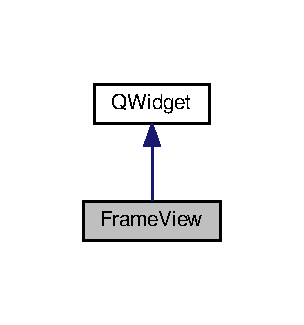
\includegraphics[width=146pt]{classGUI_1_1FrameView__inherit__graph}
\end{center}
\end{figure}
\subsection*{Public Member Functions}
\begin{DoxyCompactItemize}
\item 
\hyperlink{classGUI_1_1FrameView_a75ab7862211fa66433f92fc148ba9e7d}{Frame\+View} (\hyperlink{classGUI_1_1QWidget}{Q\+Widget} $\ast$parent=0)
\item 
\hyperlink{classGUI_1_1FrameView_a3d5c8743a83d04c10c6686dbb2698088}{void} \hyperlink{classGUI_1_1FrameView_ab38693f5302565670675156a8f33d77c}{set\+Frame} (Q\+Image \&frame)
\item 
\hyperlink{classGUI_1_1FrameView_a3d5c8743a83d04c10c6686dbb2698088}{void} \hyperlink{classGUI_1_1FrameView_ac8bb3912a3ce86b15842e79d0b421204}{clear} ()
\end{DoxyCompactItemize}
\subsection*{Protected Member Functions}
\begin{DoxyCompactItemize}
\item 
\hyperlink{classGUI_1_1FrameView_a3d5c8743a83d04c10c6686dbb2698088}{void} \hyperlink{classGUI_1_1FrameView_a6fbc07cec19868c41d513b9ef8343e9a}{resize\+Event} (Q\+Resize\+Event $\ast$event)
\item 
\hyperlink{classGUI_1_1FrameView_a3d5c8743a83d04c10c6686dbb2698088}{void} \hyperlink{classGUI_1_1FrameView_a67e5a053c3728683d415a35d1eafa5c2}{repaint\+Event} (Q\+Paint\+Event $\ast$event)
\end{DoxyCompactItemize}
\subsection*{Private Member Functions}
\begin{DoxyCompactItemize}
\item 
\hyperlink{classGUI_1_1FrameView_a3d5c8743a83d04c10c6686dbb2698088}{void} () update\+Offset()
\end{DoxyCompactItemize}
\subsection*{Private Attributes}
\begin{DoxyCompactItemize}
\item 
int \hyperlink{classGUI_1_1FrameView_a38b670313be423c4fbcaa4b6ff0e5e83}{x\+Offset}
\item 
int \hyperlink{classGUI_1_1FrameView_a016718268d32fcb95b1190cc1071e270}{y\+Offset}
\item 
Q\+Image \hyperlink{classGUI_1_1FrameView_ac300e76e226708a306ca770e1a2eac0e}{current\+Frame}
\item 
Q\+Image $\ast$ \hyperlink{classGUI_1_1FrameView_a1984b51c6b8b7444c971cbc7c6b6eead}{original\+Frame}
\end{DoxyCompactItemize}


\subsection{Detailed Description}
This class is the view used by the video player. It automatically scales the frames passed to it. 

\subsection{Constructor \& Destructor Documentation}
\hypertarget{classGUI_1_1FrameView_a75ab7862211fa66433f92fc148ba9e7d}{}\index{G\+U\+I\+::\+Frame\+View@{G\+U\+I\+::\+Frame\+View}!Frame\+View@{Frame\+View}}
\index{Frame\+View@{Frame\+View}!G\+U\+I\+::\+Frame\+View@{G\+U\+I\+::\+Frame\+View}}
\subsubsection[{Frame\+View}]{\setlength{\rightskip}{0pt plus 5cm}{\bf Frame\+View} (
\begin{DoxyParamCaption}
\item[{{\bf Q\+Widget} $\ast$}]{parent = {\ttfamily 0}}
\end{DoxyParamCaption}
)}\label{classGUI_1_1FrameView_a75ab7862211fa66433f92fc148ba9e7d}


Constructor. 



\subsection{Member Function Documentation}
\hypertarget{classGUI_1_1FrameView_ac8bb3912a3ce86b15842e79d0b421204}{}\index{G\+U\+I\+::\+Frame\+View@{G\+U\+I\+::\+Frame\+View}!clear@{clear}}
\index{clear@{clear}!G\+U\+I\+::\+Frame\+View@{G\+U\+I\+::\+Frame\+View}}
\subsubsection[{clear}]{\setlength{\rightskip}{0pt plus 5cm}{\bf void} clear (
\begin{DoxyParamCaption}
{}
\end{DoxyParamCaption}
)}\label{classGUI_1_1FrameView_ac8bb3912a3ce86b15842e79d0b421204}


Clears the current frame so nothing is shown. 

\hypertarget{classGUI_1_1FrameView_a67e5a053c3728683d415a35d1eafa5c2}{}\index{G\+U\+I\+::\+Frame\+View@{G\+U\+I\+::\+Frame\+View}!repaint\+Event@{repaint\+Event}}
\index{repaint\+Event@{repaint\+Event}!G\+U\+I\+::\+Frame\+View@{G\+U\+I\+::\+Frame\+View}}
\subsubsection[{repaint\+Event}]{\setlength{\rightskip}{0pt plus 5cm}{\bf void} repaint\+Event (
\begin{DoxyParamCaption}
\item[{Q\+Paint\+Event $\ast$}]{event}
\end{DoxyParamCaption}
)\hspace{0.3cm}{\ttfamily [protected]}}\label{classGUI_1_1FrameView_a67e5a053c3728683d415a35d1eafa5c2}


This method is called when the widget has to be repainted. 

\hypertarget{classGUI_1_1FrameView_a6fbc07cec19868c41d513b9ef8343e9a}{}\index{G\+U\+I\+::\+Frame\+View@{G\+U\+I\+::\+Frame\+View}!resize\+Event@{resize\+Event}}
\index{resize\+Event@{resize\+Event}!G\+U\+I\+::\+Frame\+View@{G\+U\+I\+::\+Frame\+View}}
\subsubsection[{resize\+Event}]{\setlength{\rightskip}{0pt plus 5cm}{\bf void} resize\+Event (
\begin{DoxyParamCaption}
\item[{Q\+Resize\+Event $\ast$}]{event}
\end{DoxyParamCaption}
)\hspace{0.3cm}{\ttfamily [protected]}}\label{classGUI_1_1FrameView_a6fbc07cec19868c41d513b9ef8343e9a}


This method is called when the widget got resized. 

\hypertarget{classGUI_1_1FrameView_ab38693f5302565670675156a8f33d77c}{}\index{G\+U\+I\+::\+Frame\+View@{G\+U\+I\+::\+Frame\+View}!set\+Frame@{set\+Frame}}
\index{set\+Frame@{set\+Frame}!G\+U\+I\+::\+Frame\+View@{G\+U\+I\+::\+Frame\+View}}
\subsubsection[{set\+Frame}]{\setlength{\rightskip}{0pt plus 5cm}{\bf void} set\+Frame (
\begin{DoxyParamCaption}
\item[{Q\+Image \&}]{frame}
\end{DoxyParamCaption}
)}\label{classGUI_1_1FrameView_ab38693f5302565670675156a8f33d77c}


Sets the frame to show. 


\begin{DoxyParams}{Parameters}
{\em frame} & The frame to show.\\
\hline
\end{DoxyParams}
\hypertarget{classGUI_1_1FrameView_a3d5c8743a83d04c10c6686dbb2698088}{}\index{G\+U\+I\+::\+Frame\+View@{G\+U\+I\+::\+Frame\+View}!void@{void}}
\index{void@{void}!G\+U\+I\+::\+Frame\+View@{G\+U\+I\+::\+Frame\+View}}
\subsubsection[{void}]{\setlength{\rightskip}{0pt plus 5cm}void (
\begin{DoxyParamCaption}
{}
\end{DoxyParamCaption}
)\hspace{0.3cm}{\ttfamily [private]}}\label{classGUI_1_1FrameView_a3d5c8743a83d04c10c6686dbb2698088}


Updates the offset at which the image is drawn. 



\subsection{Field Documentation}
\hypertarget{classGUI_1_1FrameView_ac300e76e226708a306ca770e1a2eac0e}{}\index{G\+U\+I\+::\+Frame\+View@{G\+U\+I\+::\+Frame\+View}!current\+Frame@{current\+Frame}}
\index{current\+Frame@{current\+Frame}!G\+U\+I\+::\+Frame\+View@{G\+U\+I\+::\+Frame\+View}}
\subsubsection[{current\+Frame}]{\setlength{\rightskip}{0pt plus 5cm}Q\+Image current\+Frame\hspace{0.3cm}{\ttfamily [private]}}\label{classGUI_1_1FrameView_ac300e76e226708a306ca770e1a2eac0e}
\hypertarget{classGUI_1_1FrameView_a1984b51c6b8b7444c971cbc7c6b6eead}{}\index{G\+U\+I\+::\+Frame\+View@{G\+U\+I\+::\+Frame\+View}!original\+Frame@{original\+Frame}}
\index{original\+Frame@{original\+Frame}!G\+U\+I\+::\+Frame\+View@{G\+U\+I\+::\+Frame\+View}}
\subsubsection[{original\+Frame}]{\setlength{\rightskip}{0pt plus 5cm}Q\+Image$\ast$ original\+Frame\hspace{0.3cm}{\ttfamily [private]}}\label{classGUI_1_1FrameView_a1984b51c6b8b7444c971cbc7c6b6eead}
\hypertarget{classGUI_1_1FrameView_a38b670313be423c4fbcaa4b6ff0e5e83}{}\index{G\+U\+I\+::\+Frame\+View@{G\+U\+I\+::\+Frame\+View}!x\+Offset@{x\+Offset}}
\index{x\+Offset@{x\+Offset}!G\+U\+I\+::\+Frame\+View@{G\+U\+I\+::\+Frame\+View}}
\subsubsection[{x\+Offset}]{\setlength{\rightskip}{0pt plus 5cm}int x\+Offset\hspace{0.3cm}{\ttfamily [private]}}\label{classGUI_1_1FrameView_a38b670313be423c4fbcaa4b6ff0e5e83}
\hypertarget{classGUI_1_1FrameView_a016718268d32fcb95b1190cc1071e270}{}\index{G\+U\+I\+::\+Frame\+View@{G\+U\+I\+::\+Frame\+View}!y\+Offset@{y\+Offset}}
\index{y\+Offset@{y\+Offset}!G\+U\+I\+::\+Frame\+View@{G\+U\+I\+::\+Frame\+View}}
\subsubsection[{y\+Offset}]{\setlength{\rightskip}{0pt plus 5cm}int y\+Offset\hspace{0.3cm}{\ttfamily [private]}}\label{classGUI_1_1FrameView_a016718268d32fcb95b1190cc1071e270}

\newpage\hypertarget{classGUI_1_1GlobalControlPanel}{}\section{Global\+Control\+Panel Class Reference}
\label{classGUI_1_1GlobalControlPanel}\index{Global\+Control\+Panel@{Global\+Control\+Panel}}
\subsection*{Public Member Functions}
\begin{DoxyCompactItemize}
\item 
\hypertarget{classGUI_1_1GlobalControlPanel_a6d58098c6cf63c241ed03bc797256bb1}{}void {\bfseries play} ()\label{classGUI_1_1GlobalControlPanel_a6d58098c6cf63c241ed03bc797256bb1}

\item 
\hypertarget{classGUI_1_1GlobalControlPanel_a7167f5c196fc5e167bfabde1a730e81d}{}void {\bfseries pause} ()\label{classGUI_1_1GlobalControlPanel_a7167f5c196fc5e167bfabde1a730e81d}

\item 
\hypertarget{classGUI_1_1GlobalControlPanel_a8c528baf37154d347366083f0f816846}{}void {\bfseries stop} ()\label{classGUI_1_1GlobalControlPanel_a8c528baf37154d347366083f0f816846}

\item 
\hypertarget{classGUI_1_1GlobalControlPanel_a365329da56f8b07f8c95027ba967bbc3}{}void {\bfseries next\+Frame} ()\label{classGUI_1_1GlobalControlPanel_a365329da56f8b07f8c95027ba967bbc3}

\item 
\hypertarget{classGUI_1_1GlobalControlPanel_a3c96ed37c70ebc0b32c527a04e1536d1}{}void {\bfseries previous\+Frame} ()\label{classGUI_1_1GlobalControlPanel_a3c96ed37c70ebc0b32c527a04e1536d1}

\item 
\hypertarget{classGUI_1_1GlobalControlPanel_a1aa68f77243229daea38d59bc5145d35}{}void {\bfseries set\+Position} (int position)\label{classGUI_1_1GlobalControlPanel_a1aa68f77243229daea38d59bc5145d35}

\item 
\hypertarget{classGUI_1_1GlobalControlPanel_ae13c7f95f1ceda0fec18d18c3d7619f6}{}void {\bfseries update\+Ui} ()\label{classGUI_1_1GlobalControlPanel_ae13c7f95f1ceda0fec18d18c3d7619f6}

\end{DoxyCompactItemize}
\subsection*{Data Fields}
\begin{DoxyCompactItemize}
\item 
\hypertarget{classGUI_1_1GlobalControlPanel_a360a35388d458c292758e61a66d77674}{}\hyperlink{classGUI_1_1AnalysisTab}{G\+U\+I\+::\+Analysis\+Tab} $\ast$ {\bfseries global\+Control\+Panel}\label{classGUI_1_1GlobalControlPanel_a360a35388d458c292758e61a66d77674}

\end{DoxyCompactItemize}
\subsection*{Additional Inherited Members}

\newpage\hypertarget{classModel_1_1Graph}{}\section{Graph Class Reference}
\label{classModel_1_1Graph}\index{Graph@{Graph}}
\subsection*{Public Member Functions}
\begin{DoxyCompactItemize}
\item 
\hyperlink{classModel_1_1Graph_afc5ef9d72cc2c509814200791eaef62c}{Graph} ()
\item 
void \hyperlink{classModel_1_1Graph_ad4f64ac7b49c53bcfe6e62f538381a50}{add\+Value} (int x, double y)
\item 
void \hyperlink{classModel_1_1Graph_a940d481971e87001c6e4c17585b41a8e}{cut} (int x)
\item 
double \hyperlink{classModel_1_1Graph_aacd99feb76afec4bc9bdf645d4585880}{get\+Value} (int x)
\item 
int \hyperlink{classModel_1_1Graph_aab0d4bbd0884d04dbe281cc2b9d21206}{get\+Length} ()
\item 
void \hyperlink{classModel_1_1Graph_a88400b56c971065fc52ce8c02ecaffcd}{remove\+Value} (int x)
\end{DoxyCompactItemize}
\subsection*{Data Fields}
\begin{DoxyCompactItemize}
\item 
\hyperlink{classModel_1_1EncodedVideo}{Model\+::\+Encoded\+Video} $\ast$ \hyperlink{classModel_1_1Graph_a340d02df4a8d3c909b9242c450c2c4fa}{bitrate}
\item 
\hyperlink{classModel_1_1EncodedVideo}{Model\+::\+Encoded\+Video} $\ast$ \hyperlink{classModel_1_1Graph_a6476f7924ca1e0e066bbb0da6f5ea5de}{psnr}
\item 
\hyperlink{classModel_1_1EncodedVideo}{Model\+::\+Encoded\+Video} $\ast$ \hyperlink{classModel_1_1Graph_a826dee34980905d4300038e1ebc8efaf}{red\+Histo}
\item 
\hyperlink{classModel_1_1EncodedVideo}{Model\+::\+Encoded\+Video} $\ast$ \hyperlink{classModel_1_1Graph_adb7c23252690d5783f98e23046f785e8}{green\+Histo}
\item 
\hyperlink{classModel_1_1EncodedVideo}{Model\+::\+Encoded\+Video} $\ast$ \hyperlink{classModel_1_1Graph_a478d40084049d5801d2c7c70a4447133}{blue\+Hiso}
\end{DoxyCompactItemize}
\subsection*{Private Attributes}
\begin{DoxyCompactItemize}
\item 
vector$<$ double $>$ \hyperlink{classModel_1_1Graph_abfc9d4190e850ffe8624574f41dcc757}{graph}
\end{DoxyCompactItemize}


\subsection{Detailed Description}
This class is a graph. 

\subsection{Constructor \& Destructor Documentation}
\hypertarget{classModel_1_1Graph_afc5ef9d72cc2c509814200791eaef62c}{}\index{Model\+::\+Graph@{Model\+::\+Graph}!Graph@{Graph}}
\index{Graph@{Graph}!Model\+::\+Graph@{Model\+::\+Graph}}
\subsubsection[{Graph}]{\setlength{\rightskip}{0pt plus 5cm}{\bf Graph} (
\begin{DoxyParamCaption}
{}
\end{DoxyParamCaption}
)}\label{classModel_1_1Graph_afc5ef9d72cc2c509814200791eaef62c}


Constructor. 



\subsection{Member Function Documentation}
\hypertarget{classModel_1_1Graph_ad4f64ac7b49c53bcfe6e62f538381a50}{}\index{Model\+::\+Graph@{Model\+::\+Graph}!add\+Value@{add\+Value}}
\index{add\+Value@{add\+Value}!Model\+::\+Graph@{Model\+::\+Graph}}
\subsubsection[{add\+Value}]{\setlength{\rightskip}{0pt plus 5cm}void add\+Value (
\begin{DoxyParamCaption}
\item[{int}]{x, }
\item[{double}]{y}
\end{DoxyParamCaption}
)}\label{classModel_1_1Graph_ad4f64ac7b49c53bcfe6e62f538381a50}


Adds a value pair. 


\begin{DoxyParams}{Parameters}
{\em x} & Value on the x-\/axes.\\
\hline
{\em y} & Value on the y-\/axes.\\
\hline
\end{DoxyParams}
\hypertarget{classModel_1_1Graph_a940d481971e87001c6e4c17585b41a8e}{}\index{Model\+::\+Graph@{Model\+::\+Graph}!cut@{cut}}
\index{cut@{cut}!Model\+::\+Graph@{Model\+::\+Graph}}
\subsubsection[{cut}]{\setlength{\rightskip}{0pt plus 5cm}void cut (
\begin{DoxyParamCaption}
\item[{int}]{x}
\end{DoxyParamCaption}
)}\label{classModel_1_1Graph_a940d481971e87001c6e4c17585b41a8e}


Cuts the number of vectors down up to a certain value x. 


\begin{DoxyParams}{Parameters}
{\em x} & The last x-\/value in the cut down vectors.\\
\hline
\end{DoxyParams}
\hypertarget{classModel_1_1Graph_aab0d4bbd0884d04dbe281cc2b9d21206}{}\index{Model\+::\+Graph@{Model\+::\+Graph}!get\+Length@{get\+Length}}
\index{get\+Length@{get\+Length}!Model\+::\+Graph@{Model\+::\+Graph}}
\subsubsection[{get\+Length}]{\setlength{\rightskip}{0pt plus 5cm}int get\+Length (
\begin{DoxyParamCaption}
{}
\end{DoxyParamCaption}
)}\label{classModel_1_1Graph_aab0d4bbd0884d04dbe281cc2b9d21206}


Returns the biggest x value. 

\begin{DoxyReturn}{Returns}
The biggest x value.
\end{DoxyReturn}
\hypertarget{classModel_1_1Graph_aacd99feb76afec4bc9bdf645d4585880}{}\index{Model\+::\+Graph@{Model\+::\+Graph}!get\+Value@{get\+Value}}
\index{get\+Value@{get\+Value}!Model\+::\+Graph@{Model\+::\+Graph}}
\subsubsection[{get\+Value}]{\setlength{\rightskip}{0pt plus 5cm}double get\+Value (
\begin{DoxyParamCaption}
\item[{int}]{x}
\end{DoxyParamCaption}
)}\label{classModel_1_1Graph_aacd99feb76afec4bc9bdf645d4585880}


Returns the y-\/value to a specific x-\/value. 


\begin{DoxyParams}{Parameters}
{\em x} & The x value.\\
\hline
\end{DoxyParams}
\hypertarget{classModel_1_1Graph_a88400b56c971065fc52ce8c02ecaffcd}{}\index{Model\+::\+Graph@{Model\+::\+Graph}!remove\+Value@{remove\+Value}}
\index{remove\+Value@{remove\+Value}!Model\+::\+Graph@{Model\+::\+Graph}}
\subsubsection[{remove\+Value}]{\setlength{\rightskip}{0pt plus 5cm}void remove\+Value (
\begin{DoxyParamCaption}
\item[{int}]{x}
\end{DoxyParamCaption}
)}\label{classModel_1_1Graph_a88400b56c971065fc52ce8c02ecaffcd}


Removes the corresponding y value. 


\begin{DoxyParams}{Parameters}
{\em x} & The x value whose y value shall be removed.\\
\hline
\end{DoxyParams}


\subsection{Field Documentation}
\hypertarget{classModel_1_1Graph_a340d02df4a8d3c909b9242c450c2c4fa}{}\index{Model\+::\+Graph@{Model\+::\+Graph}!bitrate@{bitrate}}
\index{bitrate@{bitrate}!Model\+::\+Graph@{Model\+::\+Graph}}
\subsubsection[{bitrate}]{\setlength{\rightskip}{0pt plus 5cm}{\bf Model\+::\+Encoded\+Video}$\ast$ bitrate}\label{classModel_1_1Graph_a340d02df4a8d3c909b9242c450c2c4fa}
\hypertarget{classModel_1_1Graph_a478d40084049d5801d2c7c70a4447133}{}\index{Model\+::\+Graph@{Model\+::\+Graph}!blue\+Hiso@{blue\+Hiso}}
\index{blue\+Hiso@{blue\+Hiso}!Model\+::\+Graph@{Model\+::\+Graph}}
\subsubsection[{blue\+Hiso}]{\setlength{\rightskip}{0pt plus 5cm}{\bf Model\+::\+Encoded\+Video}$\ast$ blue\+Hiso}\label{classModel_1_1Graph_a478d40084049d5801d2c7c70a4447133}
\hypertarget{classModel_1_1Graph_abfc9d4190e850ffe8624574f41dcc757}{}\index{Model\+::\+Graph@{Model\+::\+Graph}!graph@{graph}}
\index{graph@{graph}!Model\+::\+Graph@{Model\+::\+Graph}}
\subsubsection[{graph}]{\setlength{\rightskip}{0pt plus 5cm}vector$<$double$>$ graph\hspace{0.3cm}{\ttfamily [private]}}\label{classModel_1_1Graph_abfc9d4190e850ffe8624574f41dcc757}
\hypertarget{classModel_1_1Graph_adb7c23252690d5783f98e23046f785e8}{}\index{Model\+::\+Graph@{Model\+::\+Graph}!green\+Histo@{green\+Histo}}
\index{green\+Histo@{green\+Histo}!Model\+::\+Graph@{Model\+::\+Graph}}
\subsubsection[{green\+Histo}]{\setlength{\rightskip}{0pt plus 5cm}{\bf Model\+::\+Encoded\+Video}$\ast$ green\+Histo}\label{classModel_1_1Graph_adb7c23252690d5783f98e23046f785e8}
\hypertarget{classModel_1_1Graph_a6476f7924ca1e0e066bbb0da6f5ea5de}{}\index{Model\+::\+Graph@{Model\+::\+Graph}!psnr@{psnr}}
\index{psnr@{psnr}!Model\+::\+Graph@{Model\+::\+Graph}}
\subsubsection[{psnr}]{\setlength{\rightskip}{0pt plus 5cm}{\bf Model\+::\+Encoded\+Video}$\ast$ psnr}\label{classModel_1_1Graph_a6476f7924ca1e0e066bbb0da6f5ea5de}
\hypertarget{classModel_1_1Graph_a826dee34980905d4300038e1ebc8efaf}{}\index{Model\+::\+Graph@{Model\+::\+Graph}!red\+Histo@{red\+Histo}}
\index{red\+Histo@{red\+Histo}!Model\+::\+Graph@{Model\+::\+Graph}}
\subsubsection[{red\+Histo}]{\setlength{\rightskip}{0pt plus 5cm}{\bf Model\+::\+Encoded\+Video}$\ast$ red\+Histo}\label{classModel_1_1Graph_a826dee34980905d4300038e1ebc8efaf}

\newpage\hypertarget{classGUI_1_1GraphWidget}{}\section{Graph\+Widget Class Reference}
\label{classGUI_1_1GraphWidget}\index{Graph\+Widget@{Graph\+Widget}}
\subsection*{Public Member Functions}
\begin{DoxyCompactItemize}
\item 
\hyperlink{classGUI_1_1GraphWidget_a6d80d51caf0aee4c148baee49978f8c3}{Graph\+Widget} ()
\item 
void \hyperlink{classGUI_1_1GraphWidget_a25c17e8ca0168048e36c347f423ed017}{draw\+Graph} (\hyperlink{classModel_1_1Graph}{Model\+::\+Graph} graph, bool filled)
\item 
void \hyperlink{classGUI_1_1GraphWidget_ac7a4a8dd961c4b9c732ef22bfb4143ce}{set\+Line\+Color} (Q\+Rgb color)
\item 
void \hyperlink{classGUI_1_1GraphWidget_a7d8af579d2c285a372ec5bc60cbac4c1}{set\+Fill\+Color} (Q\+Rgb color)
\item 
\hypertarget{classGUI_1_1GraphWidget_a7b9e0f55d4f00ec543cc714478104c80}{}void {\bfseries set\+Control\+Panel} (\hyperlink{classGUI_1_1GlobalControlPanel}{G\+U\+I\+::\+Global\+Control\+Panel} $\ast$panel)\label{classGUI_1_1GraphWidget_a7b9e0f55d4f00ec543cc714478104c80}

\end{DoxyCompactItemize}
\subsection*{Data Fields}
\begin{DoxyCompactItemize}
\item 
\hypertarget{classGUI_1_1GraphWidget_a8eb06e20b4d45dae183529cdbcfccd37}{}\hyperlink{classGUI_1_1AnalysisBox}{G\+U\+I\+::\+Analysis\+Box} $\ast$ {\bfseries psnr\+Graph}\label{classGUI_1_1GraphWidget_a8eb06e20b4d45dae183529cdbcfccd37}

\item 
\hypertarget{classGUI_1_1GraphWidget_a0820983260f94179618b2d20660fccb8}{}\hyperlink{classGUI_1_1AnalysisBox}{G\+U\+I\+::\+Analysis\+Box} $\ast$ {\bfseries bitrate\+Graph}\label{classGUI_1_1GraphWidget_a0820983260f94179618b2d20660fccb8}

\item 
\hypertarget{classGUI_1_1GraphWidget_abbcef0fcdc2fe6a2fcf4f1c7dc894616}{}\hyperlink{classGUI_1_1AnalysisBox}{G\+U\+I\+::\+Analysis\+Box} $\ast$ {\bfseries red\+Histogramm}\label{classGUI_1_1GraphWidget_abbcef0fcdc2fe6a2fcf4f1c7dc894616}

\item 
\hypertarget{classGUI_1_1GraphWidget_ae1216a2a17f8e93ec56dadca439499e2}{}\hyperlink{classGUI_1_1AnalysisBox}{G\+U\+I\+::\+Analysis\+Box} $\ast$ {\bfseries blue\+Histogramm}\label{classGUI_1_1GraphWidget_ae1216a2a17f8e93ec56dadca439499e2}

\item 
\hypertarget{classGUI_1_1GraphWidget_a262e4b4b63ed00cb7e29d0e80096cc48}{}\hyperlink{classGUI_1_1AnalysisBox}{G\+U\+I\+::\+Analysis\+Box} $\ast$ {\bfseries green\+Histogramm}\label{classGUI_1_1GraphWidget_a262e4b4b63ed00cb7e29d0e80096cc48}

\item 
\hypertarget{classGUI_1_1GraphWidget_ab3ea51551e457dd2373457329db2651e}{}\hyperlink{classModel_1_1Graph}{Model\+::\+Graph} $\ast$ {\bfseries graph}\label{classGUI_1_1GraphWidget_ab3ea51551e457dd2373457329db2651e}

\end{DoxyCompactItemize}


\subsection{Detailed Description}
This class is a widget to draw graphs. 

\subsection{Constructor \& Destructor Documentation}
\hypertarget{classGUI_1_1GraphWidget_a6d80d51caf0aee4c148baee49978f8c3}{}\index{G\+U\+I\+::\+Graph\+Widget@{G\+U\+I\+::\+Graph\+Widget}!Graph\+Widget@{Graph\+Widget}}
\index{Graph\+Widget@{Graph\+Widget}!G\+U\+I\+::\+Graph\+Widget@{G\+U\+I\+::\+Graph\+Widget}}
\subsubsection[{Graph\+Widget}]{\setlength{\rightskip}{0pt plus 5cm}{\bf Graph\+Widget} (
\begin{DoxyParamCaption}
{}
\end{DoxyParamCaption}
)}\label{classGUI_1_1GraphWidget_a6d80d51caf0aee4c148baee49978f8c3}


Constructor. 



\subsection{Member Function Documentation}
\hypertarget{classGUI_1_1GraphWidget_a25c17e8ca0168048e36c347f423ed017}{}\index{G\+U\+I\+::\+Graph\+Widget@{G\+U\+I\+::\+Graph\+Widget}!draw\+Graph@{draw\+Graph}}
\index{draw\+Graph@{draw\+Graph}!G\+U\+I\+::\+Graph\+Widget@{G\+U\+I\+::\+Graph\+Widget}}
\subsubsection[{draw\+Graph}]{\setlength{\rightskip}{0pt plus 5cm}void draw\+Graph (
\begin{DoxyParamCaption}
\item[{{\bf Model\+::\+Graph}}]{graph, }
\item[{bool}]{filled}
\end{DoxyParamCaption}
)}\label{classGUI_1_1GraphWidget_a25c17e8ca0168048e36c347f423ed017}


Draws a graph to the widget. 

\hypertarget{classGUI_1_1GraphWidget_a7d8af579d2c285a372ec5bc60cbac4c1}{}\index{G\+U\+I\+::\+Graph\+Widget@{G\+U\+I\+::\+Graph\+Widget}!set\+Fill\+Color@{set\+Fill\+Color}}
\index{set\+Fill\+Color@{set\+Fill\+Color}!G\+U\+I\+::\+Graph\+Widget@{G\+U\+I\+::\+Graph\+Widget}}
\subsubsection[{set\+Fill\+Color}]{\setlength{\rightskip}{0pt plus 5cm}void set\+Fill\+Color (
\begin{DoxyParamCaption}
\item[{Q\+Rgb}]{color}
\end{DoxyParamCaption}
)}\label{classGUI_1_1GraphWidget_a7d8af579d2c285a372ec5bc60cbac4c1}


Determines the color of the area beneath the graph line. 


\begin{DoxyParams}{Parameters}
{\em color} & The color in which the area beneath the graph line is filled.\\
\hline
\end{DoxyParams}
\hypertarget{classGUI_1_1GraphWidget_ac7a4a8dd961c4b9c732ef22bfb4143ce}{}\index{G\+U\+I\+::\+Graph\+Widget@{G\+U\+I\+::\+Graph\+Widget}!set\+Line\+Color@{set\+Line\+Color}}
\index{set\+Line\+Color@{set\+Line\+Color}!G\+U\+I\+::\+Graph\+Widget@{G\+U\+I\+::\+Graph\+Widget}}
\subsubsection[{set\+Line\+Color}]{\setlength{\rightskip}{0pt plus 5cm}void set\+Line\+Color (
\begin{DoxyParamCaption}
\item[{Q\+Rgb}]{color}
\end{DoxyParamCaption}
)}\label{classGUI_1_1GraphWidget_ac7a4a8dd961c4b9c732ef22bfb4143ce}


Determines the color of the graph line. 


\begin{DoxyParams}{Parameters}
{\em color} & The color in which the line is shown.\\
\hline
\end{DoxyParams}

\newpage\hypertarget{classModel_1_1GridFilter}{}\section{Grid\+Filter Class Reference}
\label{classModel_1_1GridFilter}\index{Grid\+Filter@{Grid\+Filter}}


Inheritance diagram for Grid\+Filter\+:
\nopagebreak
\begin{figure}[H]
\begin{center}
\leavevmode
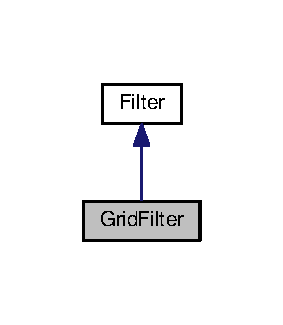
\includegraphics[width=136pt]{classModel_1_1GridFilter__inherit__graph}
\end{center}
\end{figure}
\subsection*{Public Member Functions}
\begin{DoxyCompactItemize}
\item 
\hyperlink{classModel_1_1GridFilter_ab1ae2f8274ae2f189885458ea8107430}{Grid\+Filter} ()
\item 
string \hyperlink{classModel_1_1GridFilter_a62b7b60e24f92234393b840b35808e06}{get\+Filter\+Description} ()
\item 
int \hyperlink{classModel_1_1GridFilter_abcc18b0863e36589ecfc558674efac58}{get\+Horizontal\+Lines} ()
\item 
void \hyperlink{classModel_1_1GridFilter_a849b1116004a7d70012a0b2b435a654d}{set\+Horizontal\+Lines} (int \hyperlink{classModel_1_1GridFilter_a7036f87b4b74d4ef89ef62d91f7a1db1}{horizontal\+Lines})
\item 
int \hyperlink{classModel_1_1GridFilter_ac85296b9435ef3afd4439122f5251e3e}{get\+Vertical\+Lines} ()
\item 
void \hyperlink{classModel_1_1GridFilter_a19a37598a2c1297a657d072776eb0cda}{set\+Vertical\+Lines} (int \hyperlink{classModel_1_1GridFilter_a654be30b1c42567ae3e92cbe3bf55a5c}{vertical\+Lines})
\item 
Q\+Rgb \hyperlink{classModel_1_1GridFilter_ae697defefbdf5f895406269b15758d91}{get\+Color} ()
\item 
void \hyperlink{classModel_1_1GridFilter_ad858846447f303e473dc8004ef607666}{set\+Color} (Q\+Rgb \hyperlink{classModel_1_1GridFilter_a6e0c08bd2043c82b2e837117d811db91}{color})
\item 
int \hyperlink{classModel_1_1GridFilter_ab6b7bfb33162f992d1bb4e8d6699abef}{get\+Thickness} ()
\item 
void \hyperlink{classModel_1_1GridFilter_ae2faef96ee1277d229d6b6988c66e6d3}{set\+Thickness} (int \hyperlink{classModel_1_1GridFilter_a4ae4bed5e7efe23b97dad176fe6524c3}{thickness})
\item 
int \hyperlink{classModel_1_1GridFilter_a0c8618c617e65d5ab8400704bbc09ed1}{get\+Opacity} ()
\item 
void \hyperlink{classModel_1_1GridFilter_a22b140225648b55b27f2330938ae4006}{set\+Opacity} (int \hyperlink{classModel_1_1GridFilter_ab86f8ec3f0949a133a694bba7f166a05}{opacity})
\item 
string \hyperlink{classModel_1_1GridFilter_a11335e13e50af74108bf926dc1340b4b}{get\+Name} ()
\end{DoxyCompactItemize}
\subsection*{Private Attributes}
\begin{DoxyCompactItemize}
\item 
int \hyperlink{classModel_1_1GridFilter_a7036f87b4b74d4ef89ef62d91f7a1db1}{horizontal\+Lines}
\item 
int \hyperlink{classModel_1_1GridFilter_a654be30b1c42567ae3e92cbe3bf55a5c}{vertical\+Lines}
\item 
Q\+Rgb \hyperlink{classModel_1_1GridFilter_a6e0c08bd2043c82b2e837117d811db91}{color}
\item 
int \hyperlink{classModel_1_1GridFilter_a4ae4bed5e7efe23b97dad176fe6524c3}{thickness}
\item 
int \hyperlink{classModel_1_1GridFilter_ab86f8ec3f0949a133a694bba7f166a05}{opacity}
\end{DoxyCompactItemize}
\subsection*{Additional Inherited Members}


\subsection{Detailed Description}
Inserts a grid into the video as an overlay. 

\subsection{Constructor \& Destructor Documentation}
\hypertarget{classModel_1_1GridFilter_ab1ae2f8274ae2f189885458ea8107430}{}\index{Model\+::\+Grid\+Filter@{Model\+::\+Grid\+Filter}!Grid\+Filter@{Grid\+Filter}}
\index{Grid\+Filter@{Grid\+Filter}!Model\+::\+Grid\+Filter@{Model\+::\+Grid\+Filter}}
\subsubsection[{Grid\+Filter}]{\setlength{\rightskip}{0pt plus 5cm}{\bf Grid\+Filter} (
\begin{DoxyParamCaption}
{}
\end{DoxyParamCaption}
)}\label{classModel_1_1GridFilter_ab1ae2f8274ae2f189885458ea8107430}


Constructor. 



\subsection{Member Function Documentation}
\hypertarget{classModel_1_1GridFilter_ae697defefbdf5f895406269b15758d91}{}\index{Model\+::\+Grid\+Filter@{Model\+::\+Grid\+Filter}!get\+Color@{get\+Color}}
\index{get\+Color@{get\+Color}!Model\+::\+Grid\+Filter@{Model\+::\+Grid\+Filter}}
\subsubsection[{get\+Color}]{\setlength{\rightskip}{0pt plus 5cm}Q\+Rgb get\+Color (
\begin{DoxyParamCaption}
{}
\end{DoxyParamCaption}
)}\label{classModel_1_1GridFilter_ae697defefbdf5f895406269b15758d91}


Returns the color of the grid. 

\begin{DoxyReturn}{Returns}
The gridcolor.
\end{DoxyReturn}
\hypertarget{classModel_1_1GridFilter_a62b7b60e24f92234393b840b35808e06}{}\index{Model\+::\+Grid\+Filter@{Model\+::\+Grid\+Filter}!get\+Filter\+Description@{get\+Filter\+Description}}
\index{get\+Filter\+Description@{get\+Filter\+Description}!Model\+::\+Grid\+Filter@{Model\+::\+Grid\+Filter}}
\subsubsection[{get\+Filter\+Description}]{\setlength{\rightskip}{0pt plus 5cm}string get\+Filter\+Description (
\begin{DoxyParamCaption}
{}
\end{DoxyParamCaption}
)\hspace{0.3cm}{\ttfamily [virtual]}}\label{classModel_1_1GridFilter_a62b7b60e24f92234393b840b35808e06}


Returns the string that the ffmpeg library needs to apply the filter to a video. 

\begin{DoxyReturn}{Returns}
The string for the ffmpeg library.
\end{DoxyReturn}


Implements \hyperlink{classModel_1_1Filter_a453fcafa809afa1ce58d9ef95d5f26c0}{Filter}.

\hypertarget{classModel_1_1GridFilter_abcc18b0863e36589ecfc558674efac58}{}\index{Model\+::\+Grid\+Filter@{Model\+::\+Grid\+Filter}!get\+Horizontal\+Lines@{get\+Horizontal\+Lines}}
\index{get\+Horizontal\+Lines@{get\+Horizontal\+Lines}!Model\+::\+Grid\+Filter@{Model\+::\+Grid\+Filter}}
\subsubsection[{get\+Horizontal\+Lines}]{\setlength{\rightskip}{0pt plus 5cm}int get\+Horizontal\+Lines (
\begin{DoxyParamCaption}
{}
\end{DoxyParamCaption}
)}\label{classModel_1_1GridFilter_abcc18b0863e36589ecfc558674efac58}


Returns the number of horizontal drawn lines. 

\begin{DoxyReturn}{Returns}
Number of horizontal lines.
\end{DoxyReturn}
\hypertarget{classModel_1_1GridFilter_a11335e13e50af74108bf926dc1340b4b}{}\index{Model\+::\+Grid\+Filter@{Model\+::\+Grid\+Filter}!get\+Name@{get\+Name}}
\index{get\+Name@{get\+Name}!Model\+::\+Grid\+Filter@{Model\+::\+Grid\+Filter}}
\subsubsection[{get\+Name}]{\setlength{\rightskip}{0pt plus 5cm}string get\+Name (
\begin{DoxyParamCaption}
{}
\end{DoxyParamCaption}
)\hspace{0.3cm}{\ttfamily [virtual]}}\label{classModel_1_1GridFilter_a11335e13e50af74108bf926dc1340b4b}


Returns the name of the filter. 

\begin{DoxyReturn}{Returns}
The filtername.
\end{DoxyReturn}


Implements \hyperlink{classModel_1_1Filter_ade93aa98c68d185a9c03784d36140225}{Filter}.

\hypertarget{classModel_1_1GridFilter_a0c8618c617e65d5ab8400704bbc09ed1}{}\index{Model\+::\+Grid\+Filter@{Model\+::\+Grid\+Filter}!get\+Opacity@{get\+Opacity}}
\index{get\+Opacity@{get\+Opacity}!Model\+::\+Grid\+Filter@{Model\+::\+Grid\+Filter}}
\subsubsection[{get\+Opacity}]{\setlength{\rightskip}{0pt plus 5cm}int get\+Opacity (
\begin{DoxyParamCaption}
{}
\end{DoxyParamCaption}
)}\label{classModel_1_1GridFilter_a0c8618c617e65d5ab8400704bbc09ed1}


Returns the opacity of the grid. 

\begin{DoxyReturn}{Returns}
The grids opacity.
\end{DoxyReturn}
\hypertarget{classModel_1_1GridFilter_ab6b7bfb33162f992d1bb4e8d6699abef}{}\index{Model\+::\+Grid\+Filter@{Model\+::\+Grid\+Filter}!get\+Thickness@{get\+Thickness}}
\index{get\+Thickness@{get\+Thickness}!Model\+::\+Grid\+Filter@{Model\+::\+Grid\+Filter}}
\subsubsection[{get\+Thickness}]{\setlength{\rightskip}{0pt plus 5cm}int get\+Thickness (
\begin{DoxyParamCaption}
{}
\end{DoxyParamCaption}
)}\label{classModel_1_1GridFilter_ab6b7bfb33162f992d1bb4e8d6699abef}


Returns the thickness of the drawn lines. 

\begin{DoxyReturn}{Returns}
The line thickness.
\end{DoxyReturn}
\hypertarget{classModel_1_1GridFilter_ac85296b9435ef3afd4439122f5251e3e}{}\index{Model\+::\+Grid\+Filter@{Model\+::\+Grid\+Filter}!get\+Vertical\+Lines@{get\+Vertical\+Lines}}
\index{get\+Vertical\+Lines@{get\+Vertical\+Lines}!Model\+::\+Grid\+Filter@{Model\+::\+Grid\+Filter}}
\subsubsection[{get\+Vertical\+Lines}]{\setlength{\rightskip}{0pt plus 5cm}int get\+Vertical\+Lines (
\begin{DoxyParamCaption}
{}
\end{DoxyParamCaption}
)}\label{classModel_1_1GridFilter_ac85296b9435ef3afd4439122f5251e3e}


Returns the number of vertical drawn lines. 

\begin{DoxyReturn}{Returns}
Number of vertical lines.
\end{DoxyReturn}
\hypertarget{classModel_1_1GridFilter_ad858846447f303e473dc8004ef607666}{}\index{Model\+::\+Grid\+Filter@{Model\+::\+Grid\+Filter}!set\+Color@{set\+Color}}
\index{set\+Color@{set\+Color}!Model\+::\+Grid\+Filter@{Model\+::\+Grid\+Filter}}
\subsubsection[{set\+Color}]{\setlength{\rightskip}{0pt plus 5cm}void set\+Color (
\begin{DoxyParamCaption}
\item[{Q\+Rgb}]{color}
\end{DoxyParamCaption}
)}\label{classModel_1_1GridFilter_ad858846447f303e473dc8004ef607666}


Sets the color of the grid. 


\begin{DoxyParams}{Parameters}
{\em color} & The gridcolor.\\
\hline
\end{DoxyParams}
\hypertarget{classModel_1_1GridFilter_a849b1116004a7d70012a0b2b435a654d}{}\index{Model\+::\+Grid\+Filter@{Model\+::\+Grid\+Filter}!set\+Horizontal\+Lines@{set\+Horizontal\+Lines}}
\index{set\+Horizontal\+Lines@{set\+Horizontal\+Lines}!Model\+::\+Grid\+Filter@{Model\+::\+Grid\+Filter}}
\subsubsection[{set\+Horizontal\+Lines}]{\setlength{\rightskip}{0pt plus 5cm}void set\+Horizontal\+Lines (
\begin{DoxyParamCaption}
\item[{int}]{horizontal\+Lines}
\end{DoxyParamCaption}
)}\label{classModel_1_1GridFilter_a849b1116004a7d70012a0b2b435a654d}


Sets the number of horizontal drawn lines. 


\begin{DoxyParams}{Parameters}
{\em horizontal\+Lines} & Number of horizontal lines.\\
\hline
\end{DoxyParams}
\hypertarget{classModel_1_1GridFilter_a22b140225648b55b27f2330938ae4006}{}\index{Model\+::\+Grid\+Filter@{Model\+::\+Grid\+Filter}!set\+Opacity@{set\+Opacity}}
\index{set\+Opacity@{set\+Opacity}!Model\+::\+Grid\+Filter@{Model\+::\+Grid\+Filter}}
\subsubsection[{set\+Opacity}]{\setlength{\rightskip}{0pt plus 5cm}void set\+Opacity (
\begin{DoxyParamCaption}
\item[{int}]{opacity}
\end{DoxyParamCaption}
)}\label{classModel_1_1GridFilter_a22b140225648b55b27f2330938ae4006}


Sets the opacity of the grid. 


\begin{DoxyParams}{Parameters}
{\em opacity} & The grids opacity.\\
\hline
\end{DoxyParams}
\hypertarget{classModel_1_1GridFilter_ae2faef96ee1277d229d6b6988c66e6d3}{}\index{Model\+::\+Grid\+Filter@{Model\+::\+Grid\+Filter}!set\+Thickness@{set\+Thickness}}
\index{set\+Thickness@{set\+Thickness}!Model\+::\+Grid\+Filter@{Model\+::\+Grid\+Filter}}
\subsubsection[{set\+Thickness}]{\setlength{\rightskip}{0pt plus 5cm}void set\+Thickness (
\begin{DoxyParamCaption}
\item[{int}]{thickness}
\end{DoxyParamCaption}
)}\label{classModel_1_1GridFilter_ae2faef96ee1277d229d6b6988c66e6d3}


Sets the thickness of the drawn lines. 


\begin{DoxyParams}{Parameters}
{\em thickness} & The thickness of the drawn lines.\\
\hline
\end{DoxyParams}
\hypertarget{classModel_1_1GridFilter_a19a37598a2c1297a657d072776eb0cda}{}\index{Model\+::\+Grid\+Filter@{Model\+::\+Grid\+Filter}!set\+Vertical\+Lines@{set\+Vertical\+Lines}}
\index{set\+Vertical\+Lines@{set\+Vertical\+Lines}!Model\+::\+Grid\+Filter@{Model\+::\+Grid\+Filter}}
\subsubsection[{set\+Vertical\+Lines}]{\setlength{\rightskip}{0pt plus 5cm}void set\+Vertical\+Lines (
\begin{DoxyParamCaption}
\item[{int}]{vertical\+Lines}
\end{DoxyParamCaption}
)}\label{classModel_1_1GridFilter_a19a37598a2c1297a657d072776eb0cda}


Sets the number of vertical drawn lines. 


\begin{DoxyParams}{Parameters}
{\em vertical\+Lines} & Number of vertical drawn lines.\\
\hline
\end{DoxyParams}


\subsection{Field Documentation}
\hypertarget{classModel_1_1GridFilter_a6e0c08bd2043c82b2e837117d811db91}{}\index{Model\+::\+Grid\+Filter@{Model\+::\+Grid\+Filter}!color@{color}}
\index{color@{color}!Model\+::\+Grid\+Filter@{Model\+::\+Grid\+Filter}}
\subsubsection[{color}]{\setlength{\rightskip}{0pt plus 5cm}Q\+Rgb color\hspace{0.3cm}{\ttfamily [private]}}\label{classModel_1_1GridFilter_a6e0c08bd2043c82b2e837117d811db91}
\hypertarget{classModel_1_1GridFilter_a7036f87b4b74d4ef89ef62d91f7a1db1}{}\index{Model\+::\+Grid\+Filter@{Model\+::\+Grid\+Filter}!horizontal\+Lines@{horizontal\+Lines}}
\index{horizontal\+Lines@{horizontal\+Lines}!Model\+::\+Grid\+Filter@{Model\+::\+Grid\+Filter}}
\subsubsection[{horizontal\+Lines}]{\setlength{\rightskip}{0pt plus 5cm}int horizontal\+Lines\hspace{0.3cm}{\ttfamily [private]}}\label{classModel_1_1GridFilter_a7036f87b4b74d4ef89ef62d91f7a1db1}
\hypertarget{classModel_1_1GridFilter_ab86f8ec3f0949a133a694bba7f166a05}{}\index{Model\+::\+Grid\+Filter@{Model\+::\+Grid\+Filter}!opacity@{opacity}}
\index{opacity@{opacity}!Model\+::\+Grid\+Filter@{Model\+::\+Grid\+Filter}}
\subsubsection[{opacity}]{\setlength{\rightskip}{0pt plus 5cm}int opacity\hspace{0.3cm}{\ttfamily [private]}}\label{classModel_1_1GridFilter_ab86f8ec3f0949a133a694bba7f166a05}
\hypertarget{classModel_1_1GridFilter_a4ae4bed5e7efe23b97dad176fe6524c3}{}\index{Model\+::\+Grid\+Filter@{Model\+::\+Grid\+Filter}!thickness@{thickness}}
\index{thickness@{thickness}!Model\+::\+Grid\+Filter@{Model\+::\+Grid\+Filter}}
\subsubsection[{thickness}]{\setlength{\rightskip}{0pt plus 5cm}int thickness\hspace{0.3cm}{\ttfamily [private]}}\label{classModel_1_1GridFilter_a4ae4bed5e7efe23b97dad176fe6524c3}
\hypertarget{classModel_1_1GridFilter_a654be30b1c42567ae3e92cbe3bf55a5c}{}\index{Model\+::\+Grid\+Filter@{Model\+::\+Grid\+Filter}!vertical\+Lines@{vertical\+Lines}}
\index{vertical\+Lines@{vertical\+Lines}!Model\+::\+Grid\+Filter@{Model\+::\+Grid\+Filter}}
\subsubsection[{vertical\+Lines}]{\setlength{\rightskip}{0pt plus 5cm}int vertical\+Lines\hspace{0.3cm}{\ttfamily [private]}}\label{classModel_1_1GridFilter_a654be30b1c42567ae3e92cbe3bf55a5c}

\newpage\hypertarget{classGUI_1_1GridFilterBox}{}\section{Grid\+Filter\+Box Class Reference}
\label{classGUI_1_1GridFilterBox}\index{Grid\+Filter\+Box@{Grid\+Filter\+Box}}
\subsection*{Public Member Functions}
\begin{DoxyCompactItemize}
\item 
\hyperlink{classGUI_1_1GridFilterBox_a34cd17872c955362a349743e0b2f90ee}{Grid\+Filter\+Box} (\hyperlink{classGUI_1_1Player_1_1QWidget}{G\+U\+I\+::\+Player\+::\+Q\+Widget} $\ast$parent)
\end{DoxyCompactItemize}
\subsection*{Additional Inherited Members}


\subsection{Detailed Description}
This class contains the gui elements for changing the options of a grid filter. 

\subsection{Constructor \& Destructor Documentation}
\hypertarget{classGUI_1_1GridFilterBox_a34cd17872c955362a349743e0b2f90ee}{}\index{G\+U\+I\+::\+Grid\+Filter\+Box@{G\+U\+I\+::\+Grid\+Filter\+Box}!Grid\+Filter\+Box@{Grid\+Filter\+Box}}
\index{Grid\+Filter\+Box@{Grid\+Filter\+Box}!G\+U\+I\+::\+Grid\+Filter\+Box@{G\+U\+I\+::\+Grid\+Filter\+Box}}
\subsubsection[{Grid\+Filter\+Box}]{\setlength{\rightskip}{0pt plus 5cm}{\bf Grid\+Filter\+Box} (
\begin{DoxyParamCaption}
\item[{{\bf G\+U\+I\+::\+Player\+::\+Q\+Widget} $\ast$}]{parent}
\end{DoxyParamCaption}
)}\label{classGUI_1_1GridFilterBox_a34cd17872c955362a349743e0b2f90ee}


Constructor. 


\newpage\hypertarget{classUndoRedo_1_1LoadAnalysisVideo}{}\section{Load\+Analysis\+Video Class Reference}
\label{classUndoRedo_1_1LoadAnalysisVideo}\index{Load\+Analysis\+Video@{Load\+Analysis\+Video}}


Inheritance diagram for Load\+Analysis\+Video\+:
\nopagebreak
\begin{figure}[H]
\begin{center}
\leavevmode
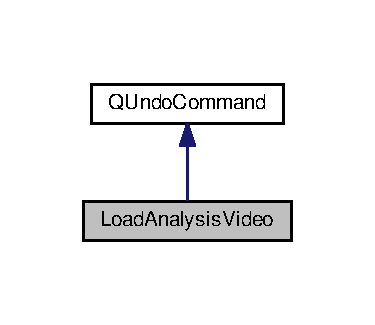
\includegraphics[width=180pt]{classUndoRedo_1_1LoadAnalysisVideo__inherit__graph}
\end{center}
\end{figure}
\subsection*{Public Member Functions}
\begin{DoxyCompactItemize}
\item 
\hyperlink{classUndoRedo_1_1LoadAnalysisVideo_ae34179e8d6121bb4cbe36e1cad9a829f}{Load\+Analysis\+Video} (\hyperlink{classGUI_1_1AnalysisTab}{G\+U\+I\+::\+Analysis\+Tab} $\ast$\hyperlink{classUndoRedo_1_1LoadAnalysisVideo_a7873b9caa261d4d8f973627c7ee4008e}{ana\+Tab}, Analyse\+Tab\+Memento ana\+Tab\+Mem, \hyperlink{classModel_1_1YuvVideo}{Model\+::\+Yuv\+Video} \hyperlink{classUndoRedo_1_1LoadAnalysisVideo_a17d20420106e047a53677d26c8db0d48}{video})
\item 
void \hyperlink{classUndoRedo_1_1LoadAnalysisVideo_a0e1e7804a53f6d62efc72c9bdbec8571}{undo} ()
\item 
void \hyperlink{classUndoRedo_1_1LoadAnalysisVideo_a93c48d6ed036e1a381be53ac67643284}{redo} ()
\end{DoxyCompactItemize}
\subsection*{Data Fields}
\begin{DoxyCompactItemize}
\item 
\hyperlink{classMemento_1_1AnalysisTabMemento}{Memento\+::\+Analysis\+Tab\+Memento} $\ast$ \hyperlink{classUndoRedo_1_1LoadAnalysisVideo_a56e13226ed93b1cf23903379eb5d89cb}{memento}
\end{DoxyCompactItemize}
\subsection*{Private Attributes}
\begin{DoxyCompactItemize}
\item 
\hyperlink{classGUI_1_1AnalysisTab}{G\+U\+I\+::\+Analysis\+Tab} $\ast$ \hyperlink{classUndoRedo_1_1LoadAnalysisVideo_a7873b9caa261d4d8f973627c7ee4008e}{ana\+Tab}
\item 
\hyperlink{classModel_1_1YuvVideo}{Model\+::\+Yuv\+Video} $\ast$ \hyperlink{classUndoRedo_1_1LoadAnalysisVideo_a17d20420106e047a53677d26c8db0d48}{video}
\end{DoxyCompactItemize}


\subsection{Detailed Description}
This class is the undo command for loading the raw video on the analysis tab. 

\subsection{Constructor \& Destructor Documentation}
\hypertarget{classUndoRedo_1_1LoadAnalysisVideo_ae34179e8d6121bb4cbe36e1cad9a829f}{}\index{Undo\+Redo\+::\+Load\+Analysis\+Video@{Undo\+Redo\+::\+Load\+Analysis\+Video}!Load\+Analysis\+Video@{Load\+Analysis\+Video}}
\index{Load\+Analysis\+Video@{Load\+Analysis\+Video}!Undo\+Redo\+::\+Load\+Analysis\+Video@{Undo\+Redo\+::\+Load\+Analysis\+Video}}
\subsubsection[{Load\+Analysis\+Video}]{\setlength{\rightskip}{0pt plus 5cm}{\bf Load\+Analysis\+Video} (
\begin{DoxyParamCaption}
\item[{{\bf G\+U\+I\+::\+Analysis\+Tab} $\ast$}]{ana\+Tab, }
\item[{Analyse\+Tab\+Memento}]{ana\+Tab\+Mem, }
\item[{{\bf Model\+::\+Yuv\+Video}}]{video}
\end{DoxyParamCaption}
)}\label{classUndoRedo_1_1LoadAnalysisVideo_ae34179e8d6121bb4cbe36e1cad9a829f}


Constructor.. 


\begin{DoxyParams}{Parameters}
{\em ana\+Tab} & The Analyse\+Tab to operate on.\\
\hline
{\em ana\+Tab\+Mem} & The memento of the analyse tab before the raw video is loaded.\\
\hline
{\em video} & The new raw video.\\
\hline
\end{DoxyParams}


\subsection{Member Function Documentation}
\hypertarget{classUndoRedo_1_1LoadAnalysisVideo_a93c48d6ed036e1a381be53ac67643284}{}\index{Undo\+Redo\+::\+Load\+Analysis\+Video@{Undo\+Redo\+::\+Load\+Analysis\+Video}!redo@{redo}}
\index{redo@{redo}!Undo\+Redo\+::\+Load\+Analysis\+Video@{Undo\+Redo\+::\+Load\+Analysis\+Video}}
\subsubsection[{redo}]{\setlength{\rightskip}{0pt plus 5cm}void redo (
\begin{DoxyParamCaption}
{}
\end{DoxyParamCaption}
)}\label{classUndoRedo_1_1LoadAnalysisVideo_a93c48d6ed036e1a381be53ac67643284}


Loads anew raw video in the analysis tab. 

\hypertarget{classUndoRedo_1_1LoadAnalysisVideo_a0e1e7804a53f6d62efc72c9bdbec8571}{}\index{Undo\+Redo\+::\+Load\+Analysis\+Video@{Undo\+Redo\+::\+Load\+Analysis\+Video}!undo@{undo}}
\index{undo@{undo}!Undo\+Redo\+::\+Load\+Analysis\+Video@{Undo\+Redo\+::\+Load\+Analysis\+Video}}
\subsubsection[{undo}]{\setlength{\rightskip}{0pt plus 5cm}void undo (
\begin{DoxyParamCaption}
{}
\end{DoxyParamCaption}
)}\label{classUndoRedo_1_1LoadAnalysisVideo_a0e1e7804a53f6d62efc72c9bdbec8571}


Restores the anlysis tab to the state before the new video was loaded. 



\subsection{Field Documentation}
\hypertarget{classUndoRedo_1_1LoadAnalysisVideo_a7873b9caa261d4d8f973627c7ee4008e}{}\index{Undo\+Redo\+::\+Load\+Analysis\+Video@{Undo\+Redo\+::\+Load\+Analysis\+Video}!ana\+Tab@{ana\+Tab}}
\index{ana\+Tab@{ana\+Tab}!Undo\+Redo\+::\+Load\+Analysis\+Video@{Undo\+Redo\+::\+Load\+Analysis\+Video}}
\subsubsection[{ana\+Tab}]{\setlength{\rightskip}{0pt plus 5cm}{\bf G\+U\+I\+::\+Analysis\+Tab}$\ast$ ana\+Tab\hspace{0.3cm}{\ttfamily [private]}}\label{classUndoRedo_1_1LoadAnalysisVideo_a7873b9caa261d4d8f973627c7ee4008e}
\hypertarget{classUndoRedo_1_1LoadAnalysisVideo_a56e13226ed93b1cf23903379eb5d89cb}{}\index{Undo\+Redo\+::\+Load\+Analysis\+Video@{Undo\+Redo\+::\+Load\+Analysis\+Video}!memento@{memento}}
\index{memento@{memento}!Undo\+Redo\+::\+Load\+Analysis\+Video@{Undo\+Redo\+::\+Load\+Analysis\+Video}}
\subsubsection[{memento}]{\setlength{\rightskip}{0pt plus 5cm}{\bf Memento\+::\+Analysis\+Tab\+Memento}$\ast$ memento}\label{classUndoRedo_1_1LoadAnalysisVideo_a56e13226ed93b1cf23903379eb5d89cb}
\hypertarget{classUndoRedo_1_1LoadAnalysisVideo_a17d20420106e047a53677d26c8db0d48}{}\index{Undo\+Redo\+::\+Load\+Analysis\+Video@{Undo\+Redo\+::\+Load\+Analysis\+Video}!video@{video}}
\index{video@{video}!Undo\+Redo\+::\+Load\+Analysis\+Video@{Undo\+Redo\+::\+Load\+Analysis\+Video}}
\subsubsection[{video}]{\setlength{\rightskip}{0pt plus 5cm}{\bf Model\+::\+Yuv\+Video}$\ast$ video\hspace{0.3cm}{\ttfamily [private]}}\label{classUndoRedo_1_1LoadAnalysisVideo_a17d20420106e047a53677d26c8db0d48}

\newpage\hypertarget{classUndoRedo_1_1LoadFilterconfig}{}\section{Load\+Filterconfig Class Reference}
\label{classUndoRedo_1_1LoadFilterconfig}\index{Load\+Filterconfig@{Load\+Filterconfig}}
\subsection*{Public Member Functions}
\begin{DoxyCompactItemize}
\item 
\hyperlink{classUndoRedo_1_1LoadFilterconfig_a7d0074b786381d2cf9d31f7ec9ef4924}{Load\+Filterconfig} (\hyperlink{classGUI_1_1FilterTab}{G\+U\+I\+::\+Filter\+Tab} $\ast$filter\+Tab, \hyperlink{classModel_1_1Filter_1_1FilterList}{Model\+::\+Filter\+::\+Filter\+List} old\+List, \hyperlink{classModel_1_1Filter_1_1FilterList}{Model\+::\+Filter\+::\+Filter\+List} list)
\item 
void \hyperlink{classUndoRedo_1_1LoadFilterconfig_a0e1e7804a53f6d62efc72c9bdbec8571}{undo} ()
\item 
void \hyperlink{classUndoRedo_1_1LoadFilterconfig_a93c48d6ed036e1a381be53ac67643284}{redo} ()
\end{DoxyCompactItemize}


\subsection{Detailed Description}
This class is the undo command for loading a filter config on the filter tab. 

\subsection{Constructor \& Destructor Documentation}
\hypertarget{classUndoRedo_1_1LoadFilterconfig_a7d0074b786381d2cf9d31f7ec9ef4924}{}\index{Undo\+Redo\+::\+Load\+Filterconfig@{Undo\+Redo\+::\+Load\+Filterconfig}!Load\+Filterconfig@{Load\+Filterconfig}}
\index{Load\+Filterconfig@{Load\+Filterconfig}!Undo\+Redo\+::\+Load\+Filterconfig@{Undo\+Redo\+::\+Load\+Filterconfig}}
\subsubsection[{Load\+Filterconfig}]{\setlength{\rightskip}{0pt plus 5cm}{\bf Load\+Filterconfig} (
\begin{DoxyParamCaption}
\item[{{\bf G\+U\+I\+::\+Filter\+Tab} $\ast$}]{filter\+Tab, }
\item[{{\bf Model\+::\+Filter\+::\+Filter\+List}}]{old\+List, }
\item[{{\bf Model\+::\+Filter\+::\+Filter\+List}}]{list}
\end{DoxyParamCaption}
)}\label{classUndoRedo_1_1LoadFilterconfig_a7d0074b786381d2cf9d31f7ec9ef4924}


Constuctor. 


\begin{DoxyParams}{Parameters}
{\em filter\+Tab} & The filtertab to operate on.\\
\hline
{\em old\+List} & The filterlist before the config is loaded.\\
\hline
{\em list} & The new filter configuration.\\
\hline
\end{DoxyParams}


\subsection{Member Function Documentation}
\hypertarget{classUndoRedo_1_1LoadFilterconfig_a93c48d6ed036e1a381be53ac67643284}{}\index{Undo\+Redo\+::\+Load\+Filterconfig@{Undo\+Redo\+::\+Load\+Filterconfig}!redo@{redo}}
\index{redo@{redo}!Undo\+Redo\+::\+Load\+Filterconfig@{Undo\+Redo\+::\+Load\+Filterconfig}}
\subsubsection[{redo}]{\setlength{\rightskip}{0pt plus 5cm}void redo (
\begin{DoxyParamCaption}
{}
\end{DoxyParamCaption}
)}\label{classUndoRedo_1_1LoadFilterconfig_a93c48d6ed036e1a381be53ac67643284}


Loads a filter configuration from a external file. 

\hypertarget{classUndoRedo_1_1LoadFilterconfig_a0e1e7804a53f6d62efc72c9bdbec8571}{}\index{Undo\+Redo\+::\+Load\+Filterconfig@{Undo\+Redo\+::\+Load\+Filterconfig}!undo@{undo}}
\index{undo@{undo}!Undo\+Redo\+::\+Load\+Filterconfig@{Undo\+Redo\+::\+Load\+Filterconfig}}
\subsubsection[{undo}]{\setlength{\rightskip}{0pt plus 5cm}void undo (
\begin{DoxyParamCaption}
{}
\end{DoxyParamCaption}
)}\label{classUndoRedo_1_1LoadFilterconfig_a0e1e7804a53f6d62efc72c9bdbec8571}


Loads the filter configuration present before external configuration was loaded. 


\newpage\hypertarget{classUndoRedo_1_1LoadFilterVideo}{}\section{Load\+Filter\+Video Class Reference}
\label{classUndoRedo_1_1LoadFilterVideo}\index{Load\+Filter\+Video@{Load\+Filter\+Video}}
\subsection*{Public Member Functions}
\begin{DoxyCompactItemize}
\item 
\hyperlink{classUndoRedo_1_1LoadFilterVideo_a0f1e769b2aae8de0c0872a5167e6efa2}{Load\+Filter\+Video} (\hyperlink{classGUI_1_1FilterTab}{G\+U\+I\+::\+Filter\+Tab} $\ast$filter\+Tab, \hyperlink{classModel_1_1YuvVideo}{Model\+::\+Yuv\+Video} video, \hyperlink{classMemento_1_1FilterTabMemento}{Memento\+::\+Filter\+Tab\+Memento} memento)
\item 
void \hyperlink{classUndoRedo_1_1LoadFilterVideo_a0e1e7804a53f6d62efc72c9bdbec8571}{undo} ()
\item 
void \hyperlink{classUndoRedo_1_1LoadFilterVideo_a93c48d6ed036e1a381be53ac67643284}{redo} ()
\end{DoxyCompactItemize}


\subsection{Detailed Description}
This class is the undo command for loading a raw video in the filtertab. 

\subsection{Constructor \& Destructor Documentation}
\hypertarget{classUndoRedo_1_1LoadFilterVideo_a0f1e769b2aae8de0c0872a5167e6efa2}{}\index{Undo\+Redo\+::\+Load\+Filter\+Video@{Undo\+Redo\+::\+Load\+Filter\+Video}!Load\+Filter\+Video@{Load\+Filter\+Video}}
\index{Load\+Filter\+Video@{Load\+Filter\+Video}!Undo\+Redo\+::\+Load\+Filter\+Video@{Undo\+Redo\+::\+Load\+Filter\+Video}}
\subsubsection[{Load\+Filter\+Video}]{\setlength{\rightskip}{0pt plus 5cm}{\bf Load\+Filter\+Video} (
\begin{DoxyParamCaption}
\item[{{\bf G\+U\+I\+::\+Filter\+Tab} $\ast$}]{filter\+Tab, }
\item[{{\bf Model\+::\+Yuv\+Video}}]{video, }
\item[{{\bf Memento\+::\+Filter\+Tab\+Memento}}]{memento}
\end{DoxyParamCaption}
)}\label{classUndoRedo_1_1LoadFilterVideo_a0f1e769b2aae8de0c0872a5167e6efa2}


Constuctor. 


\begin{DoxyParams}{Parameters}
{\em filter\+Tab} & The filtertab to operate on.\\
\hline
{\em video} & The video to use.\\
\hline
{\em memento} & The memento before the new video is loaded.\\
\hline
\end{DoxyParams}


\subsection{Member Function Documentation}
\hypertarget{classUndoRedo_1_1LoadFilterVideo_a93c48d6ed036e1a381be53ac67643284}{}\index{Undo\+Redo\+::\+Load\+Filter\+Video@{Undo\+Redo\+::\+Load\+Filter\+Video}!redo@{redo}}
\index{redo@{redo}!Undo\+Redo\+::\+Load\+Filter\+Video@{Undo\+Redo\+::\+Load\+Filter\+Video}}
\subsubsection[{redo}]{\setlength{\rightskip}{0pt plus 5cm}void redo (
\begin{DoxyParamCaption}
{}
\end{DoxyParamCaption}
)}\label{classUndoRedo_1_1LoadFilterVideo_a93c48d6ed036e1a381be53ac67643284}


Loads video to which filter can be applied. 

\hypertarget{classUndoRedo_1_1LoadFilterVideo_a0e1e7804a53f6d62efc72c9bdbec8571}{}\index{Undo\+Redo\+::\+Load\+Filter\+Video@{Undo\+Redo\+::\+Load\+Filter\+Video}!undo@{undo}}
\index{undo@{undo}!Undo\+Redo\+::\+Load\+Filter\+Video@{Undo\+Redo\+::\+Load\+Filter\+Video}}
\subsubsection[{undo}]{\setlength{\rightskip}{0pt plus 5cm}void undo (
\begin{DoxyParamCaption}
{}
\end{DoxyParamCaption}
)}\label{classUndoRedo_1_1LoadFilterVideo_a0e1e7804a53f6d62efc72c9bdbec8571}


Removes current video to which filters can be applied and loads previous video. 


\newpage\hypertarget{classUtility_1_1MacroblockCalculator}{}\section{Macroblock\+Calculator Class Reference}
\label{classUtility_1_1MacroblockCalculator}\index{Macroblock\+Calculator@{Macroblock\+Calculator}}
\subsection*{Public Member Functions}
\begin{DoxyCompactItemize}
\item 
void \hyperlink{classUtility_1_1MacroblockCalculator_a64fd3d3ae21bac78ee0465eb2bd51469}{macro\+Block\+Calculator} (\hyperlink{classModel_1_1AVVideo}{Model\+::\+A\+V\+Video} \&video)
\item 
void \hyperlink{classUtility_1_1MacroblockCalculator_ad52940f86e4a7a034a3a8f43edb584c9}{calculate\+Macroblock\+Images} (\hyperlink{classGUI_1_1Player_1_1Video}{G\+U\+I\+::\+Player\+::\+Video} \&target)
\end{DoxyCompactItemize}


\subsection{Detailed Description}
This class calculates the macroblocks of a video. 

\subsection{Member Function Documentation}
\hypertarget{classUtility_1_1MacroblockCalculator_ad52940f86e4a7a034a3a8f43edb584c9}{}\index{Utility\+::\+Macroblock\+Calculator@{Utility\+::\+Macroblock\+Calculator}!calculate\+Macroblock\+Images@{calculate\+Macroblock\+Images}}
\index{calculate\+Macroblock\+Images@{calculate\+Macroblock\+Images}!Utility\+::\+Macroblock\+Calculator@{Utility\+::\+Macroblock\+Calculator}}
\subsubsection[{calculate\+Macroblock\+Images}]{\setlength{\rightskip}{0pt plus 5cm}void calculate\+Macroblock\+Images (
\begin{DoxyParamCaption}
\item[{{\bf G\+U\+I\+::\+Player\+::\+Video} \&}]{target}
\end{DoxyParamCaption}
)}\label{classUtility_1_1MacroblockCalculator_ad52940f86e4a7a034a3a8f43edb584c9}


Calculates Q\+Image video with macroblock overlay. 


\begin{DoxyParams}{Parameters}
{\em target} & the video the frames with the calculated macroblocks are added to\\
\hline
\end{DoxyParams}
\hypertarget{classUtility_1_1MacroblockCalculator_a64fd3d3ae21bac78ee0465eb2bd51469}{}\index{Utility\+::\+Macroblock\+Calculator@{Utility\+::\+Macroblock\+Calculator}!macro\+Block\+Calculator@{macro\+Block\+Calculator}}
\index{macro\+Block\+Calculator@{macro\+Block\+Calculator}!Utility\+::\+Macroblock\+Calculator@{Utility\+::\+Macroblock\+Calculator}}
\subsubsection[{macro\+Block\+Calculator}]{\setlength{\rightskip}{0pt plus 5cm}void macro\+Block\+Calculator (
\begin{DoxyParamCaption}
\item[{{\bf Model\+::\+A\+V\+Video} \&}]{video}
\end{DoxyParamCaption}
)}\label{classUtility_1_1MacroblockCalculator_a64fd3d3ae21bac78ee0465eb2bd51469}


Constructor. 


\begin{DoxyParams}{Parameters}
{\em video} & the video to calculate the macroblocks for\\
\hline
\end{DoxyParams}

\newpage\hypertarget{classGUI_1_1MainWindow}{}\section{Main\+Window Class Reference}
\label{classGUI_1_1MainWindow}\index{Main\+Window@{Main\+Window}}


Inheritance diagram for Main\+Window\+:
\nopagebreak
\begin{figure}[H]
\begin{center}
\leavevmode
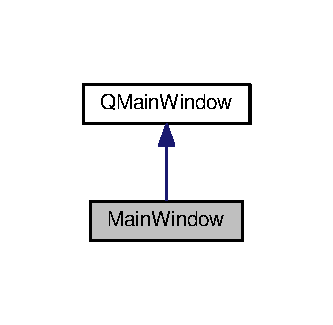
\includegraphics[width=160pt]{classGUI_1_1MainWindow__inherit__graph}
\end{center}
\end{figure}
\subsection*{Public Member Functions}
\begin{DoxyCompactItemize}
\item 
\hyperlink{classGUI_1_1MainWindow_aafaf72c52e0a059620d80026737865b4}{Main\+Window} (\hyperlink{classGUI_1_1QWidget}{G\+U\+I\+::\+Q\+Widget} $\ast$parent)
\item 
\hyperlink{classMemento_1_1MainWindowMemento}{Memento\+::\+Main\+Window\+Memento} \hyperlink{classGUI_1_1MainWindow_ae085d92d1c5bec057a813bd86bc20fa4}{get\+Memento} ()
\item 
void \hyperlink{classGUI_1_1MainWindow_a72db05f1394dbeeb2a76b74d8f65917b}{restore} (\hyperlink{classMemento_1_1MainWindowMemento}{Memento\+::\+Main\+Window\+Memento} memento)
\item 
\hyperlink{classModel_1_1Project}{Model\+::\+Project} \& \hyperlink{classGUI_1_1MainWindow_a0e9fe41bc141b89f4955329b959310eb}{get\+Project} ()
\end{DoxyCompactItemize}
\subsection*{Data Fields}
\begin{DoxyCompactItemize}
\item 
\hyperlink{classModel_1_1Project}{Model\+::\+Project} $\ast$ \hyperlink{classGUI_1_1MainWindow_a870e96d05ee2e8c616461952d01ac408}{loaded\+Project}
\end{DoxyCompactItemize}
\subsection*{Private Member Functions}
\begin{DoxyCompactItemize}
\item 
void \hyperlink{classGUI_1_1MainWindow_ae128dfd6fbafee0370f9912e4112f054}{new\+Project} ()
\item 
void \hyperlink{classGUI_1_1MainWindow_a0e1e7804a53f6d62efc72c9bdbec8571}{undo} ()
\item 
void \hyperlink{classGUI_1_1MainWindow_a65005f9a81d8c7396e2583a80a1f70bf}{save\+As} ()
\item 
void \hyperlink{classGUI_1_1MainWindow_adb575720306afca2c0e0c5930467321b}{load\+Project} ()
\item 
void \hyperlink{classGUI_1_1MainWindow_a5de2650de39370a5fe89f8d918966276}{save\+Project} ()
\item 
void \hyperlink{classGUI_1_1MainWindow_a93c48d6ed036e1a381be53ac67643284}{redo} ()
\item 
void \hyperlink{classGUI_1_1MainWindow_aa72182c9a958af0e87b65ab7bdba0035}{create\+Ui} ()
\item 
void \hyperlink{classGUI_1_1MainWindow_ac3ca31ff0047daecf8bbe393a15e940c}{connect\+Actions} ()
\item 
void \hyperlink{classGUI_1_1MainWindow_a5421da114e56e8856aa455426c24f805}{create\+Menu\+Bar} ()
\end{DoxyCompactItemize}
\subsection*{Private Attributes}
\begin{DoxyCompactItemize}
\item 
Q\+Status\+Bar $\ast$ \hyperlink{classGUI_1_1MainWindow_ab12bbb712331d72b3972876494b01d43}{statusbar}
\item 
Q\+Menu\+Bar $\ast$ \hyperlink{classGUI_1_1MainWindow_a3a7fd0d9d9fcaf5f23b620ecc1d868a2}{menubar\+\_\+project}
\item 
Q\+Menu\+Bar $\ast$ \hyperlink{classGUI_1_1MainWindow_a5beda12aa8191deaad381531b99992f8}{menubar\+\_\+edit}
\item 
Q\+Action $\ast$ \hyperlink{classGUI_1_1MainWindow_a5cf13e75b97a8a55f79a7f1a5dfeccdd}{action\+\_\+new\+Project}
\item 
Q\+Action $\ast$ \hyperlink{classGUI_1_1MainWindow_af4ed54c2c44d393a4c854ca626103f72}{action\+\_\+undo}
\item 
Q\+Action $\ast$ \hyperlink{classGUI_1_1MainWindow_a477f9c21e430c9db3664df4ac4a5bec9}{action\+\_\+save\+As}
\item 
Q\+Action $\ast$ \hyperlink{classGUI_1_1MainWindow_acbc3dfeebc15f93a7808e5a1d7a44492}{action\+\_\+load\+Project}
\item 
Q\+Action $\ast$ \hyperlink{classGUI_1_1MainWindow_a84cc9a3cf59e2fdd3196da97a5faa717}{action\+\_\+save\+Project}
\item 
Q\+Action $\ast$ \hyperlink{classGUI_1_1MainWindow_a76bce8131d4330008b0f40cf8e8b97d6}{action\+\_\+redo}
\item 
Q\+Tab\+Widget $\ast$ \hyperlink{classGUI_1_1MainWindow_aaeb8f9f47ba45615e767b2a7f7b009d9}{tab\+\_\+tabs}
\end{DoxyCompactItemize}


\subsection{Detailed Description}
This class is the main window that is shown. 

\subsection{Constructor \& Destructor Documentation}
\hypertarget{classGUI_1_1MainWindow_aafaf72c52e0a059620d80026737865b4}{}\index{G\+U\+I\+::\+Main\+Window@{G\+U\+I\+::\+Main\+Window}!Main\+Window@{Main\+Window}}
\index{Main\+Window@{Main\+Window}!G\+U\+I\+::\+Main\+Window@{G\+U\+I\+::\+Main\+Window}}
\subsubsection[{Main\+Window}]{\setlength{\rightskip}{0pt plus 5cm}{\bf Main\+Window} (
\begin{DoxyParamCaption}
\item[{{\bf G\+U\+I\+::\+Q\+Widget} $\ast$}]{parent}
\end{DoxyParamCaption}
)}\label{classGUI_1_1MainWindow_aafaf72c52e0a059620d80026737865b4}


Constructor. 



\subsection{Member Function Documentation}
\hypertarget{classGUI_1_1MainWindow_ac3ca31ff0047daecf8bbe393a15e940c}{}\index{G\+U\+I\+::\+Main\+Window@{G\+U\+I\+::\+Main\+Window}!connect\+Actions@{connect\+Actions}}
\index{connect\+Actions@{connect\+Actions}!G\+U\+I\+::\+Main\+Window@{G\+U\+I\+::\+Main\+Window}}
\subsubsection[{connect\+Actions}]{\setlength{\rightskip}{0pt plus 5cm}void connect\+Actions (
\begin{DoxyParamCaption}
{}
\end{DoxyParamCaption}
)\hspace{0.3cm}{\ttfamily [private]}}\label{classGUI_1_1MainWindow_ac3ca31ff0047daecf8bbe393a15e940c}


connect actions in the menu\+Bars to the slots in this class 

\hypertarget{classGUI_1_1MainWindow_a5421da114e56e8856aa455426c24f805}{}\index{G\+U\+I\+::\+Main\+Window@{G\+U\+I\+::\+Main\+Window}!create\+Menu\+Bar@{create\+Menu\+Bar}}
\index{create\+Menu\+Bar@{create\+Menu\+Bar}!G\+U\+I\+::\+Main\+Window@{G\+U\+I\+::\+Main\+Window}}
\subsubsection[{create\+Menu\+Bar}]{\setlength{\rightskip}{0pt plus 5cm}void create\+Menu\+Bar (
\begin{DoxyParamCaption}
{}
\end{DoxyParamCaption}
)\hspace{0.3cm}{\ttfamily [private]}}\label{classGUI_1_1MainWindow_a5421da114e56e8856aa455426c24f805}
\hypertarget{classGUI_1_1MainWindow_aa72182c9a958af0e87b65ab7bdba0035}{}\index{G\+U\+I\+::\+Main\+Window@{G\+U\+I\+::\+Main\+Window}!create\+Ui@{create\+Ui}}
\index{create\+Ui@{create\+Ui}!G\+U\+I\+::\+Main\+Window@{G\+U\+I\+::\+Main\+Window}}
\subsubsection[{create\+Ui}]{\setlength{\rightskip}{0pt plus 5cm}void create\+Ui (
\begin{DoxyParamCaption}
{}
\end{DoxyParamCaption}
)\hspace{0.3cm}{\ttfamily [private]}}\label{classGUI_1_1MainWindow_aa72182c9a958af0e87b65ab7bdba0035}


creates the U\+I 

\hypertarget{classGUI_1_1MainWindow_ae085d92d1c5bec057a813bd86bc20fa4}{}\index{G\+U\+I\+::\+Main\+Window@{G\+U\+I\+::\+Main\+Window}!get\+Memento@{get\+Memento}}
\index{get\+Memento@{get\+Memento}!G\+U\+I\+::\+Main\+Window@{G\+U\+I\+::\+Main\+Window}}
\subsubsection[{get\+Memento}]{\setlength{\rightskip}{0pt plus 5cm}{\bf Memento\+::\+Main\+Window\+Memento} get\+Memento (
\begin{DoxyParamCaption}
{}
\end{DoxyParamCaption}
)}\label{classGUI_1_1MainWindow_ae085d92d1c5bec057a813bd86bc20fa4}


Creates a memento which contains the state of the window. 

\begin{DoxyReturn}{Returns}
The created memento.
\end{DoxyReturn}
\hypertarget{classGUI_1_1MainWindow_a0e9fe41bc141b89f4955329b959310eb}{}\index{G\+U\+I\+::\+Main\+Window@{G\+U\+I\+::\+Main\+Window}!get\+Project@{get\+Project}}
\index{get\+Project@{get\+Project}!G\+U\+I\+::\+Main\+Window@{G\+U\+I\+::\+Main\+Window}}
\subsubsection[{get\+Project}]{\setlength{\rightskip}{0pt plus 5cm}{\bf Model\+::\+Project} \& get\+Project (
\begin{DoxyParamCaption}
{}
\end{DoxyParamCaption}
)}\label{classGUI_1_1MainWindow_a0e9fe41bc141b89f4955329b959310eb}


Returns the project that is currently loaded. 

\begin{DoxyReturn}{Returns}
The currently loaded project.
\end{DoxyReturn}
\hypertarget{classGUI_1_1MainWindow_adb575720306afca2c0e0c5930467321b}{}\index{G\+U\+I\+::\+Main\+Window@{G\+U\+I\+::\+Main\+Window}!load\+Project@{load\+Project}}
\index{load\+Project@{load\+Project}!G\+U\+I\+::\+Main\+Window@{G\+U\+I\+::\+Main\+Window}}
\subsubsection[{load\+Project}]{\setlength{\rightskip}{0pt plus 5cm}void load\+Project (
\begin{DoxyParamCaption}
{}
\end{DoxyParamCaption}
)\hspace{0.3cm}{\ttfamily [private]}}\label{classGUI_1_1MainWindow_adb575720306afca2c0e0c5930467321b}


Slot\+:connected with action\+\_\+load\+Project.\+triggered() opens Q\+File\+Dialog and opens project in the selected file if possible 

\hypertarget{classGUI_1_1MainWindow_ae128dfd6fbafee0370f9912e4112f054}{}\index{G\+U\+I\+::\+Main\+Window@{G\+U\+I\+::\+Main\+Window}!new\+Project@{new\+Project}}
\index{new\+Project@{new\+Project}!G\+U\+I\+::\+Main\+Window@{G\+U\+I\+::\+Main\+Window}}
\subsubsection[{new\+Project}]{\setlength{\rightskip}{0pt plus 5cm}void new\+Project (
\begin{DoxyParamCaption}
{}
\end{DoxyParamCaption}
)\hspace{0.3cm}{\ttfamily [private]}}\label{classGUI_1_1MainWindow_ae128dfd6fbafee0370f9912e4112f054}


slot creates new project, removes existing one 

\hypertarget{classGUI_1_1MainWindow_a93c48d6ed036e1a381be53ac67643284}{}\index{G\+U\+I\+::\+Main\+Window@{G\+U\+I\+::\+Main\+Window}!redo@{redo}}
\index{redo@{redo}!G\+U\+I\+::\+Main\+Window@{G\+U\+I\+::\+Main\+Window}}
\subsubsection[{redo}]{\setlength{\rightskip}{0pt plus 5cm}void redo (
\begin{DoxyParamCaption}
{}
\end{DoxyParamCaption}
)\hspace{0.3cm}{\ttfamily [private]}}\label{classGUI_1_1MainWindow_a93c48d6ed036e1a381be53ac67643284}


Slot\+:connected with action\+\_\+redo.\+triggered() redo action if undo has been used 

\hypertarget{classGUI_1_1MainWindow_a72db05f1394dbeeb2a76b74d8f65917b}{}\index{G\+U\+I\+::\+Main\+Window@{G\+U\+I\+::\+Main\+Window}!restore@{restore}}
\index{restore@{restore}!G\+U\+I\+::\+Main\+Window@{G\+U\+I\+::\+Main\+Window}}
\subsubsection[{restore}]{\setlength{\rightskip}{0pt plus 5cm}void restore (
\begin{DoxyParamCaption}
\item[{{\bf Memento\+::\+Main\+Window\+Memento}}]{memento}
\end{DoxyParamCaption}
)}\label{classGUI_1_1MainWindow_a72db05f1394dbeeb2a76b74d8f65917b}


Restores the window based on the memento. 


\begin{DoxyParams}{Parameters}
{\em memento} & The memento which contains the state of the window.\\
\hline
\end{DoxyParams}
\hypertarget{classGUI_1_1MainWindow_a65005f9a81d8c7396e2583a80a1f70bf}{}\index{G\+U\+I\+::\+Main\+Window@{G\+U\+I\+::\+Main\+Window}!save\+As@{save\+As}}
\index{save\+As@{save\+As}!G\+U\+I\+::\+Main\+Window@{G\+U\+I\+::\+Main\+Window}}
\subsubsection[{save\+As}]{\setlength{\rightskip}{0pt plus 5cm}void save\+As (
\begin{DoxyParamCaption}
{}
\end{DoxyParamCaption}
)\hspace{0.3cm}{\ttfamily [private]}}\label{classGUI_1_1MainWindow_a65005f9a81d8c7396e2583a80a1f70bf}


Slot\+:connected with action\+\_\+save\+As.\+triggered() Opens Q\+File\+Dialog and saves project in selected file 

\hypertarget{classGUI_1_1MainWindow_a5de2650de39370a5fe89f8d918966276}{}\index{G\+U\+I\+::\+Main\+Window@{G\+U\+I\+::\+Main\+Window}!save\+Project@{save\+Project}}
\index{save\+Project@{save\+Project}!G\+U\+I\+::\+Main\+Window@{G\+U\+I\+::\+Main\+Window}}
\subsubsection[{save\+Project}]{\setlength{\rightskip}{0pt plus 5cm}void save\+Project (
\begin{DoxyParamCaption}
{}
\end{DoxyParamCaption}
)\hspace{0.3cm}{\ttfamily [private]}}\label{classGUI_1_1MainWindow_a5de2650de39370a5fe89f8d918966276}


Slot\+:connected with action\+\_\+save\+Project.\+triggered() opens Q\+File\+Dialog and saves project in selected file 

\hypertarget{classGUI_1_1MainWindow_a0e1e7804a53f6d62efc72c9bdbec8571}{}\index{G\+U\+I\+::\+Main\+Window@{G\+U\+I\+::\+Main\+Window}!undo@{undo}}
\index{undo@{undo}!G\+U\+I\+::\+Main\+Window@{G\+U\+I\+::\+Main\+Window}}
\subsubsection[{undo}]{\setlength{\rightskip}{0pt plus 5cm}void undo (
\begin{DoxyParamCaption}
{}
\end{DoxyParamCaption}
)\hspace{0.3cm}{\ttfamily [private]}}\label{classGUI_1_1MainWindow_a0e1e7804a53f6d62efc72c9bdbec8571}


Slot\+:connected with action\+\_\+undo.\+triggered() undo last action if possible 



\subsection{Field Documentation}
\hypertarget{classGUI_1_1MainWindow_acbc3dfeebc15f93a7808e5a1d7a44492}{}\index{G\+U\+I\+::\+Main\+Window@{G\+U\+I\+::\+Main\+Window}!action\+\_\+load\+Project@{action\+\_\+load\+Project}}
\index{action\+\_\+load\+Project@{action\+\_\+load\+Project}!G\+U\+I\+::\+Main\+Window@{G\+U\+I\+::\+Main\+Window}}
\subsubsection[{action\+\_\+load\+Project}]{\setlength{\rightskip}{0pt plus 5cm}Q\+Action$\ast$ action\+\_\+load\+Project\hspace{0.3cm}{\ttfamily [private]}}\label{classGUI_1_1MainWindow_acbc3dfeebc15f93a7808e5a1d7a44492}
\hypertarget{classGUI_1_1MainWindow_a5cf13e75b97a8a55f79a7f1a5dfeccdd}{}\index{G\+U\+I\+::\+Main\+Window@{G\+U\+I\+::\+Main\+Window}!action\+\_\+new\+Project@{action\+\_\+new\+Project}}
\index{action\+\_\+new\+Project@{action\+\_\+new\+Project}!G\+U\+I\+::\+Main\+Window@{G\+U\+I\+::\+Main\+Window}}
\subsubsection[{action\+\_\+new\+Project}]{\setlength{\rightskip}{0pt plus 5cm}Q\+Action$\ast$ action\+\_\+new\+Project\hspace{0.3cm}{\ttfamily [private]}}\label{classGUI_1_1MainWindow_a5cf13e75b97a8a55f79a7f1a5dfeccdd}
\hypertarget{classGUI_1_1MainWindow_a76bce8131d4330008b0f40cf8e8b97d6}{}\index{G\+U\+I\+::\+Main\+Window@{G\+U\+I\+::\+Main\+Window}!action\+\_\+redo@{action\+\_\+redo}}
\index{action\+\_\+redo@{action\+\_\+redo}!G\+U\+I\+::\+Main\+Window@{G\+U\+I\+::\+Main\+Window}}
\subsubsection[{action\+\_\+redo}]{\setlength{\rightskip}{0pt plus 5cm}Q\+Action$\ast$ action\+\_\+redo\hspace{0.3cm}{\ttfamily [private]}}\label{classGUI_1_1MainWindow_a76bce8131d4330008b0f40cf8e8b97d6}
\hypertarget{classGUI_1_1MainWindow_a477f9c21e430c9db3664df4ac4a5bec9}{}\index{G\+U\+I\+::\+Main\+Window@{G\+U\+I\+::\+Main\+Window}!action\+\_\+save\+As@{action\+\_\+save\+As}}
\index{action\+\_\+save\+As@{action\+\_\+save\+As}!G\+U\+I\+::\+Main\+Window@{G\+U\+I\+::\+Main\+Window}}
\subsubsection[{action\+\_\+save\+As}]{\setlength{\rightskip}{0pt plus 5cm}Q\+Action$\ast$ action\+\_\+save\+As\hspace{0.3cm}{\ttfamily [private]}}\label{classGUI_1_1MainWindow_a477f9c21e430c9db3664df4ac4a5bec9}
\hypertarget{classGUI_1_1MainWindow_a84cc9a3cf59e2fdd3196da97a5faa717}{}\index{G\+U\+I\+::\+Main\+Window@{G\+U\+I\+::\+Main\+Window}!action\+\_\+save\+Project@{action\+\_\+save\+Project}}
\index{action\+\_\+save\+Project@{action\+\_\+save\+Project}!G\+U\+I\+::\+Main\+Window@{G\+U\+I\+::\+Main\+Window}}
\subsubsection[{action\+\_\+save\+Project}]{\setlength{\rightskip}{0pt plus 5cm}Q\+Action$\ast$ action\+\_\+save\+Project\hspace{0.3cm}{\ttfamily [private]}}\label{classGUI_1_1MainWindow_a84cc9a3cf59e2fdd3196da97a5faa717}
\hypertarget{classGUI_1_1MainWindow_af4ed54c2c44d393a4c854ca626103f72}{}\index{G\+U\+I\+::\+Main\+Window@{G\+U\+I\+::\+Main\+Window}!action\+\_\+undo@{action\+\_\+undo}}
\index{action\+\_\+undo@{action\+\_\+undo}!G\+U\+I\+::\+Main\+Window@{G\+U\+I\+::\+Main\+Window}}
\subsubsection[{action\+\_\+undo}]{\setlength{\rightskip}{0pt plus 5cm}Q\+Action$\ast$ action\+\_\+undo\hspace{0.3cm}{\ttfamily [private]}}\label{classGUI_1_1MainWindow_af4ed54c2c44d393a4c854ca626103f72}
\hypertarget{classGUI_1_1MainWindow_a870e96d05ee2e8c616461952d01ac408}{}\index{G\+U\+I\+::\+Main\+Window@{G\+U\+I\+::\+Main\+Window}!loaded\+Project@{loaded\+Project}}
\index{loaded\+Project@{loaded\+Project}!G\+U\+I\+::\+Main\+Window@{G\+U\+I\+::\+Main\+Window}}
\subsubsection[{loaded\+Project}]{\setlength{\rightskip}{0pt plus 5cm}{\bf Model\+::\+Project}$\ast$ loaded\+Project}\label{classGUI_1_1MainWindow_a870e96d05ee2e8c616461952d01ac408}
\hypertarget{classGUI_1_1MainWindow_a5beda12aa8191deaad381531b99992f8}{}\index{G\+U\+I\+::\+Main\+Window@{G\+U\+I\+::\+Main\+Window}!menubar\+\_\+edit@{menubar\+\_\+edit}}
\index{menubar\+\_\+edit@{menubar\+\_\+edit}!G\+U\+I\+::\+Main\+Window@{G\+U\+I\+::\+Main\+Window}}
\subsubsection[{menubar\+\_\+edit}]{\setlength{\rightskip}{0pt plus 5cm}Q\+Menu\+Bar$\ast$ menubar\+\_\+edit\hspace{0.3cm}{\ttfamily [private]}}\label{classGUI_1_1MainWindow_a5beda12aa8191deaad381531b99992f8}
\hypertarget{classGUI_1_1MainWindow_a3a7fd0d9d9fcaf5f23b620ecc1d868a2}{}\index{G\+U\+I\+::\+Main\+Window@{G\+U\+I\+::\+Main\+Window}!menubar\+\_\+project@{menubar\+\_\+project}}
\index{menubar\+\_\+project@{menubar\+\_\+project}!G\+U\+I\+::\+Main\+Window@{G\+U\+I\+::\+Main\+Window}}
\subsubsection[{menubar\+\_\+project}]{\setlength{\rightskip}{0pt plus 5cm}Q\+Menu\+Bar$\ast$ menubar\+\_\+project\hspace{0.3cm}{\ttfamily [private]}}\label{classGUI_1_1MainWindow_a3a7fd0d9d9fcaf5f23b620ecc1d868a2}
\hypertarget{classGUI_1_1MainWindow_ab12bbb712331d72b3972876494b01d43}{}\index{G\+U\+I\+::\+Main\+Window@{G\+U\+I\+::\+Main\+Window}!statusbar@{statusbar}}
\index{statusbar@{statusbar}!G\+U\+I\+::\+Main\+Window@{G\+U\+I\+::\+Main\+Window}}
\subsubsection[{statusbar}]{\setlength{\rightskip}{0pt plus 5cm}Q\+Status\+Bar$\ast$ statusbar\hspace{0.3cm}{\ttfamily [private]}}\label{classGUI_1_1MainWindow_ab12bbb712331d72b3972876494b01d43}
\hypertarget{classGUI_1_1MainWindow_aaeb8f9f47ba45615e767b2a7f7b009d9}{}\index{G\+U\+I\+::\+Main\+Window@{G\+U\+I\+::\+Main\+Window}!tab\+\_\+tabs@{tab\+\_\+tabs}}
\index{tab\+\_\+tabs@{tab\+\_\+tabs}!G\+U\+I\+::\+Main\+Window@{G\+U\+I\+::\+Main\+Window}}
\subsubsection[{tab\+\_\+tabs}]{\setlength{\rightskip}{0pt plus 5cm}Q\+Tab\+Widget$\ast$ tab\+\_\+tabs\hspace{0.3cm}{\ttfamily [private]}}\label{classGUI_1_1MainWindow_aaeb8f9f47ba45615e767b2a7f7b009d9}

\newpage\hypertarget{classMemento_1_1MainWindowMemento}{}\section{Main\+Window\+Memento Class Reference}
\label{classMemento_1_1MainWindowMemento}\index{Main\+Window\+Memento@{Main\+Window\+Memento}}
\subsection*{Public Member Functions}
\begin{DoxyCompactItemize}
\item 
\hyperlink{classMemento_1_1MainWindowMemento_a2ce9d23f57fc6397812a080c3111d56c}{Main\+Window\+Memento} ()
\item 
int \hyperlink{classMemento_1_1MainWindowMemento_a876003270f9665415d49783d0669511a}{get\+Selected\+Tab} ()
\item 
void \hyperlink{classMemento_1_1MainWindowMemento_a9ec6af835d6fdbf10eb8a6db5ad59578}{set\+Selected\+Tab} (int \hyperlink{classMemento_1_1MainWindowMemento_aa1aed58bddd5b90f62a2516015ab3c04}{selected\+Tab})
\item 
\hyperlink{classMemento_1_1AnalysisTabMemento}{Memento\+::\+Analysis\+Tab\+Memento} \hyperlink{classMemento_1_1MainWindowMemento_aeaae363ca3c1aaa02d9acd9fbcd669e5}{get\+Analysis\+Tab\+Memento} ()
\item 
void \hyperlink{classMemento_1_1MainWindowMemento_a2f3cbb73b8364dfb6640b0e5225600cf}{set\+Analysis\+Tab\+Memento} (\hyperlink{classMemento_1_1AnalysisTabMemento}{Memento\+::\+Analysis\+Tab\+Memento} analysis\+Tab\+Me\+Mento)
\item 
\hyperlink{classMemento_1_1FilterTabMemento}{Memento\+::\+Filter\+Tab\+Memento} \hyperlink{classMemento_1_1MainWindowMemento_aca564eecb180bc19d899b14c9ebe5486}{get\+Filter\+Tab\+Memento} ()
\item 
void \hyperlink{classMemento_1_1MainWindowMemento_aabc5961524bfb567d2f7f5bdf79e6661}{set\+Filter\+Tab\+Memento} (\hyperlink{classMemento_1_1FilterTabMemento}{Memento\+::\+Filter\+Tab\+Memento} filter\+Tab\+Memento)
\end{DoxyCompactItemize}
\subsection*{Private Attributes}
\begin{DoxyCompactItemize}
\item 
int \hyperlink{classMemento_1_1MainWindowMemento_aa1aed58bddd5b90f62a2516015ab3c04}{selected\+Tab}
\item 
\hyperlink{classMemento_1_1AnalysisTabMemento}{Memento\+::\+Analysis\+Tab\+Memento} $\ast$ \hyperlink{classMemento_1_1MainWindowMemento_a706b928eccc0de3d1175f53e3bf6e391}{analysis\+Tab}
\item 
\hyperlink{classMemento_1_1FilterTabMemento}{Memento\+::\+Filter\+Tab\+Memento} $\ast$ \hyperlink{classMemento_1_1MainWindowMemento_aa834b7b9b12f3913750cd558db4b7796}{filter\+Tab}
\end{DoxyCompactItemize}


\subsection{Detailed Description}
This class is the memento for the Main\+Window. 

\subsection{Constructor \& Destructor Documentation}
\hypertarget{classMemento_1_1MainWindowMemento_a2ce9d23f57fc6397812a080c3111d56c}{}\index{Memento\+::\+Main\+Window\+Memento@{Memento\+::\+Main\+Window\+Memento}!Main\+Window\+Memento@{Main\+Window\+Memento}}
\index{Main\+Window\+Memento@{Main\+Window\+Memento}!Memento\+::\+Main\+Window\+Memento@{Memento\+::\+Main\+Window\+Memento}}
\subsubsection[{Main\+Window\+Memento}]{\setlength{\rightskip}{0pt plus 5cm}{\bf Main\+Window\+Memento} (
\begin{DoxyParamCaption}
{}
\end{DoxyParamCaption}
)}\label{classMemento_1_1MainWindowMemento_a2ce9d23f57fc6397812a080c3111d56c}


Constructor. 



\subsection{Member Function Documentation}
\hypertarget{classMemento_1_1MainWindowMemento_aeaae363ca3c1aaa02d9acd9fbcd669e5}{}\index{Memento\+::\+Main\+Window\+Memento@{Memento\+::\+Main\+Window\+Memento}!get\+Analysis\+Tab\+Memento@{get\+Analysis\+Tab\+Memento}}
\index{get\+Analysis\+Tab\+Memento@{get\+Analysis\+Tab\+Memento}!Memento\+::\+Main\+Window\+Memento@{Memento\+::\+Main\+Window\+Memento}}
\subsubsection[{get\+Analysis\+Tab\+Memento}]{\setlength{\rightskip}{0pt plus 5cm}{\bf Memento\+::\+Analysis\+Tab\+Memento} get\+Analysis\+Tab\+Memento (
\begin{DoxyParamCaption}
{}
\end{DoxyParamCaption}
)}\label{classMemento_1_1MainWindowMemento_aeaae363ca3c1aaa02d9acd9fbcd669e5}


Returns the \hyperlink{classMemento_1_1AnalysisTabMemento}{Analysis\+Tab\+Memento}. 

\begin{DoxyReturn}{Returns}
The \hyperlink{classMemento_1_1AnalysisTabMemento}{Analysis\+Tab\+Memento}.
\end{DoxyReturn}
\hypertarget{classMemento_1_1MainWindowMemento_aca564eecb180bc19d899b14c9ebe5486}{}\index{Memento\+::\+Main\+Window\+Memento@{Memento\+::\+Main\+Window\+Memento}!get\+Filter\+Tab\+Memento@{get\+Filter\+Tab\+Memento}}
\index{get\+Filter\+Tab\+Memento@{get\+Filter\+Tab\+Memento}!Memento\+::\+Main\+Window\+Memento@{Memento\+::\+Main\+Window\+Memento}}
\subsubsection[{get\+Filter\+Tab\+Memento}]{\setlength{\rightskip}{0pt plus 5cm}{\bf Memento\+::\+Filter\+Tab\+Memento} get\+Filter\+Tab\+Memento (
\begin{DoxyParamCaption}
{}
\end{DoxyParamCaption}
)}\label{classMemento_1_1MainWindowMemento_aca564eecb180bc19d899b14c9ebe5486}


Returns the \hyperlink{classMemento_1_1FilterTabMemento}{Filter\+Tab\+Memento}. 

\begin{DoxyReturn}{Returns}
The \hyperlink{classMemento_1_1FilterTabMemento}{Filter\+Tab\+Memento}.
\end{DoxyReturn}
\hypertarget{classMemento_1_1MainWindowMemento_a876003270f9665415d49783d0669511a}{}\index{Memento\+::\+Main\+Window\+Memento@{Memento\+::\+Main\+Window\+Memento}!get\+Selected\+Tab@{get\+Selected\+Tab}}
\index{get\+Selected\+Tab@{get\+Selected\+Tab}!Memento\+::\+Main\+Window\+Memento@{Memento\+::\+Main\+Window\+Memento}}
\subsubsection[{get\+Selected\+Tab}]{\setlength{\rightskip}{0pt plus 5cm}int get\+Selected\+Tab (
\begin{DoxyParamCaption}
{}
\end{DoxyParamCaption}
)}\label{classMemento_1_1MainWindowMemento_a876003270f9665415d49783d0669511a}


Returns the currently selected tab. 

\begin{DoxyReturn}{Returns}
The currently selected tab.
\end{DoxyReturn}
\hypertarget{classMemento_1_1MainWindowMemento_a2f3cbb73b8364dfb6640b0e5225600cf}{}\index{Memento\+::\+Main\+Window\+Memento@{Memento\+::\+Main\+Window\+Memento}!set\+Analysis\+Tab\+Memento@{set\+Analysis\+Tab\+Memento}}
\index{set\+Analysis\+Tab\+Memento@{set\+Analysis\+Tab\+Memento}!Memento\+::\+Main\+Window\+Memento@{Memento\+::\+Main\+Window\+Memento}}
\subsubsection[{set\+Analysis\+Tab\+Memento}]{\setlength{\rightskip}{0pt plus 5cm}void set\+Analysis\+Tab\+Memento (
\begin{DoxyParamCaption}
\item[{{\bf Memento\+::\+Analysis\+Tab\+Memento}}]{analysis\+Tab\+Me\+Mento}
\end{DoxyParamCaption}
)}\label{classMemento_1_1MainWindowMemento_a2f3cbb73b8364dfb6640b0e5225600cf}


Sets the \hyperlink{classMemento_1_1AnalysisTabMemento}{Analysis\+Tab\+Memento}. 


\begin{DoxyParams}{Parameters}
{\em analysis\+Tab\+Me\+Mento} & The \hyperlink{classMemento_1_1AnalysisTabMemento}{Analysis\+Tab\+Memento}.\\
\hline
\end{DoxyParams}
\hypertarget{classMemento_1_1MainWindowMemento_aabc5961524bfb567d2f7f5bdf79e6661}{}\index{Memento\+::\+Main\+Window\+Memento@{Memento\+::\+Main\+Window\+Memento}!set\+Filter\+Tab\+Memento@{set\+Filter\+Tab\+Memento}}
\index{set\+Filter\+Tab\+Memento@{set\+Filter\+Tab\+Memento}!Memento\+::\+Main\+Window\+Memento@{Memento\+::\+Main\+Window\+Memento}}
\subsubsection[{set\+Filter\+Tab\+Memento}]{\setlength{\rightskip}{0pt plus 5cm}void set\+Filter\+Tab\+Memento (
\begin{DoxyParamCaption}
\item[{{\bf Memento\+::\+Filter\+Tab\+Memento}}]{filter\+Tab\+Memento}
\end{DoxyParamCaption}
)}\label{classMemento_1_1MainWindowMemento_aabc5961524bfb567d2f7f5bdf79e6661}


Sets the \hyperlink{classMemento_1_1FilterTabMemento}{Filter\+Tab\+Memento}. 


\begin{DoxyParams}{Parameters}
{\em filter\+Tab\+Memento} & The \hyperlink{classMemento_1_1FilterTabMemento}{Filter\+Tab\+Memento}.\\
\hline
\end{DoxyParams}
\hypertarget{classMemento_1_1MainWindowMemento_a9ec6af835d6fdbf10eb8a6db5ad59578}{}\index{Memento\+::\+Main\+Window\+Memento@{Memento\+::\+Main\+Window\+Memento}!set\+Selected\+Tab@{set\+Selected\+Tab}}
\index{set\+Selected\+Tab@{set\+Selected\+Tab}!Memento\+::\+Main\+Window\+Memento@{Memento\+::\+Main\+Window\+Memento}}
\subsubsection[{set\+Selected\+Tab}]{\setlength{\rightskip}{0pt plus 5cm}void set\+Selected\+Tab (
\begin{DoxyParamCaption}
\item[{int}]{selected\+Tab}
\end{DoxyParamCaption}
)}\label{classMemento_1_1MainWindowMemento_a9ec6af835d6fdbf10eb8a6db5ad59578}


Sets the currently selected tab. 


\begin{DoxyParams}{Parameters}
{\em selected\+Tab} & The currently selected tab.\\
\hline
\end{DoxyParams}


\subsection{Field Documentation}
\hypertarget{classMemento_1_1MainWindowMemento_a706b928eccc0de3d1175f53e3bf6e391}{}\index{Memento\+::\+Main\+Window\+Memento@{Memento\+::\+Main\+Window\+Memento}!analysis\+Tab@{analysis\+Tab}}
\index{analysis\+Tab@{analysis\+Tab}!Memento\+::\+Main\+Window\+Memento@{Memento\+::\+Main\+Window\+Memento}}
\subsubsection[{analysis\+Tab}]{\setlength{\rightskip}{0pt plus 5cm}{\bf Memento\+::\+Analysis\+Tab\+Memento}$\ast$ analysis\+Tab\hspace{0.3cm}{\ttfamily [private]}}\label{classMemento_1_1MainWindowMemento_a706b928eccc0de3d1175f53e3bf6e391}
\hypertarget{classMemento_1_1MainWindowMemento_aa834b7b9b12f3913750cd558db4b7796}{}\index{Memento\+::\+Main\+Window\+Memento@{Memento\+::\+Main\+Window\+Memento}!filter\+Tab@{filter\+Tab}}
\index{filter\+Tab@{filter\+Tab}!Memento\+::\+Main\+Window\+Memento@{Memento\+::\+Main\+Window\+Memento}}
\subsubsection[{filter\+Tab}]{\setlength{\rightskip}{0pt plus 5cm}{\bf Memento\+::\+Filter\+Tab\+Memento}$\ast$ filter\+Tab\hspace{0.3cm}{\ttfamily [private]}}\label{classMemento_1_1MainWindowMemento_aa834b7b9b12f3913750cd558db4b7796}
\hypertarget{classMemento_1_1MainWindowMemento_aa1aed58bddd5b90f62a2516015ab3c04}{}\index{Memento\+::\+Main\+Window\+Memento@{Memento\+::\+Main\+Window\+Memento}!selected\+Tab@{selected\+Tab}}
\index{selected\+Tab@{selected\+Tab}!Memento\+::\+Main\+Window\+Memento@{Memento\+::\+Main\+Window\+Memento}}
\subsubsection[{selected\+Tab}]{\setlength{\rightskip}{0pt plus 5cm}int selected\+Tab\hspace{0.3cm}{\ttfamily [private]}}\label{classMemento_1_1MainWindowMemento_aa1aed58bddd5b90f62a2516015ab3c04}

\newpage\hypertarget{classModel_1_1MirrorFilter}{}\section{Mirror\+Filter Class Reference}
\label{classModel_1_1MirrorFilter}\index{Mirror\+Filter@{Mirror\+Filter}}


Inheritance diagram for Mirror\+Filter\+:
\nopagebreak
\begin{figure}[H]
\begin{center}
\leavevmode
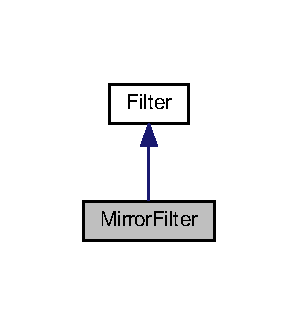
\includegraphics[width=143pt]{classModel_1_1MirrorFilter__inherit__graph}
\end{center}
\end{figure}
\subsection*{Public Member Functions}
\begin{DoxyCompactItemize}
\item 
\hyperlink{classModel_1_1MirrorFilter_a534aebee3440f56936f691affb8be0d5}{Mirror\+Filter} ()
\item 
string \hyperlink{classModel_1_1MirrorFilter_a62b7b60e24f92234393b840b35808e06}{get\+Filter\+Description} ()
\item 
string \hyperlink{classModel_1_1MirrorFilter_a11335e13e50af74108bf926dc1340b4b}{get\+Name} ()
\item 
\hyperlink{namespaceModel_a8a20195c97d8c704572b5922370c2fbc}{Model\+::\+Mirror\+Mode} \hyperlink{classModel_1_1MirrorFilter_a16d9fccd7fad368d92355882c46ee5e8}{get\+Mode} ()
\item 
void \hyperlink{classModel_1_1MirrorFilter_a1900f4cbb22c7684bd6bbce54560b90f}{set\+Mode} (\hyperlink{namespaceModel_a8a20195c97d8c704572b5922370c2fbc}{Model\+::\+Mirror\+Mode} \hyperlink{classModel_1_1MirrorFilter_ab31669960b71c1d178389716b1122a51}{mode})
\end{DoxyCompactItemize}
\subsection*{Private Attributes}
\begin{DoxyCompactItemize}
\item 
\hyperlink{namespaceModel_a8a20195c97d8c704572b5922370c2fbc}{Model\+::\+Mirror\+Mode} $\ast$ \hyperlink{classModel_1_1MirrorFilter_ab31669960b71c1d178389716b1122a51}{mode}
\end{DoxyCompactItemize}
\subsection*{Additional Inherited Members}


\subsection{Detailed Description}
Mirrors the video horizontally or vertically. 

\subsection{Constructor \& Destructor Documentation}
\hypertarget{classModel_1_1MirrorFilter_a534aebee3440f56936f691affb8be0d5}{}\index{Model\+::\+Mirror\+Filter@{Model\+::\+Mirror\+Filter}!Mirror\+Filter@{Mirror\+Filter}}
\index{Mirror\+Filter@{Mirror\+Filter}!Model\+::\+Mirror\+Filter@{Model\+::\+Mirror\+Filter}}
\subsubsection[{Mirror\+Filter}]{\setlength{\rightskip}{0pt plus 5cm}{\bf Mirror\+Filter} (
\begin{DoxyParamCaption}
{}
\end{DoxyParamCaption}
)}\label{classModel_1_1MirrorFilter_a534aebee3440f56936f691affb8be0d5}


Constructor. 



\subsection{Member Function Documentation}
\hypertarget{classModel_1_1MirrorFilter_a62b7b60e24f92234393b840b35808e06}{}\index{Model\+::\+Mirror\+Filter@{Model\+::\+Mirror\+Filter}!get\+Filter\+Description@{get\+Filter\+Description}}
\index{get\+Filter\+Description@{get\+Filter\+Description}!Model\+::\+Mirror\+Filter@{Model\+::\+Mirror\+Filter}}
\subsubsection[{get\+Filter\+Description}]{\setlength{\rightskip}{0pt plus 5cm}string get\+Filter\+Description (
\begin{DoxyParamCaption}
{}
\end{DoxyParamCaption}
)\hspace{0.3cm}{\ttfamily [virtual]}}\label{classModel_1_1MirrorFilter_a62b7b60e24f92234393b840b35808e06}


Returns the string that the ffmpeg library needs to apply the filter to a video. 

\begin{DoxyReturn}{Returns}
The string for the ffmpeg library.
\end{DoxyReturn}


Implements \hyperlink{classModel_1_1Filter_a453fcafa809afa1ce58d9ef95d5f26c0}{Filter}.

\hypertarget{classModel_1_1MirrorFilter_a16d9fccd7fad368d92355882c46ee5e8}{}\index{Model\+::\+Mirror\+Filter@{Model\+::\+Mirror\+Filter}!get\+Mode@{get\+Mode}}
\index{get\+Mode@{get\+Mode}!Model\+::\+Mirror\+Filter@{Model\+::\+Mirror\+Filter}}
\subsubsection[{get\+Mode}]{\setlength{\rightskip}{0pt plus 5cm}{\bf Model\+::\+Mirror\+Mode} get\+Mode (
\begin{DoxyParamCaption}
{}
\end{DoxyParamCaption}
)}\label{classModel_1_1MirrorFilter_a16d9fccd7fad368d92355882c46ee5e8}


Returns the Mirror\+Mode. 

\begin{DoxyReturn}{Returns}
The Mirror\+Mode.
\end{DoxyReturn}
\hypertarget{classModel_1_1MirrorFilter_a11335e13e50af74108bf926dc1340b4b}{}\index{Model\+::\+Mirror\+Filter@{Model\+::\+Mirror\+Filter}!get\+Name@{get\+Name}}
\index{get\+Name@{get\+Name}!Model\+::\+Mirror\+Filter@{Model\+::\+Mirror\+Filter}}
\subsubsection[{get\+Name}]{\setlength{\rightskip}{0pt plus 5cm}string get\+Name (
\begin{DoxyParamCaption}
{}
\end{DoxyParamCaption}
)\hspace{0.3cm}{\ttfamily [virtual]}}\label{classModel_1_1MirrorFilter_a11335e13e50af74108bf926dc1340b4b}


Returns the name of the filter. 

\begin{DoxyReturn}{Returns}
The filtername.
\end{DoxyReturn}


Implements \hyperlink{classModel_1_1Filter_ade93aa98c68d185a9c03784d36140225}{Filter}.

\hypertarget{classModel_1_1MirrorFilter_a1900f4cbb22c7684bd6bbce54560b90f}{}\index{Model\+::\+Mirror\+Filter@{Model\+::\+Mirror\+Filter}!set\+Mode@{set\+Mode}}
\index{set\+Mode@{set\+Mode}!Model\+::\+Mirror\+Filter@{Model\+::\+Mirror\+Filter}}
\subsubsection[{set\+Mode}]{\setlength{\rightskip}{0pt plus 5cm}void set\+Mode (
\begin{DoxyParamCaption}
\item[{{\bf Model\+::\+Mirror\+Mode}}]{mode}
\end{DoxyParamCaption}
)}\label{classModel_1_1MirrorFilter_a1900f4cbb22c7684bd6bbce54560b90f}


Sets the Mirror\+Mode. 


\begin{DoxyParams}{Parameters}
{\em mode} & The Mirror\+Mode.\\
\hline
\end{DoxyParams}


\subsection{Field Documentation}
\hypertarget{classModel_1_1MirrorFilter_ab31669960b71c1d178389716b1122a51}{}\index{Model\+::\+Mirror\+Filter@{Model\+::\+Mirror\+Filter}!mode@{mode}}
\index{mode@{mode}!Model\+::\+Mirror\+Filter@{Model\+::\+Mirror\+Filter}}
\subsubsection[{mode}]{\setlength{\rightskip}{0pt plus 5cm}{\bf Model\+::\+Mirror\+Mode}$\ast$ mode\hspace{0.3cm}{\ttfamily [private]}}\label{classModel_1_1MirrorFilter_ab31669960b71c1d178389716b1122a51}

\newpage\hypertarget{classGUI_1_1MirrorFilterBox}{}\section{Mirror\+Filter\+Box Class Reference}
\label{classGUI_1_1MirrorFilterBox}\index{Mirror\+Filter\+Box@{Mirror\+Filter\+Box}}
\subsection*{Public Member Functions}
\begin{DoxyCompactItemize}
\item 
\hyperlink{classGUI_1_1MirrorFilterBox_a2ca521332b6bba79b0897b1679e8af69}{Mirror\+Filter\+Box} (\hyperlink{classGUI_1_1Player_1_1QWidget}{G\+U\+I\+::\+Player\+::\+Q\+Widget} $\ast$parent)
\end{DoxyCompactItemize}
\subsection*{Additional Inherited Members}


\subsection{Detailed Description}
This class contains the gui elements for changing the options of a mirror filter. 

\subsection{Constructor \& Destructor Documentation}
\hypertarget{classGUI_1_1MirrorFilterBox_a2ca521332b6bba79b0897b1679e8af69}{}\index{G\+U\+I\+::\+Mirror\+Filter\+Box@{G\+U\+I\+::\+Mirror\+Filter\+Box}!Mirror\+Filter\+Box@{Mirror\+Filter\+Box}}
\index{Mirror\+Filter\+Box@{Mirror\+Filter\+Box}!G\+U\+I\+::\+Mirror\+Filter\+Box@{G\+U\+I\+::\+Mirror\+Filter\+Box}}
\subsubsection[{Mirror\+Filter\+Box}]{\setlength{\rightskip}{0pt plus 5cm}{\bf Mirror\+Filter\+Box} (
\begin{DoxyParamCaption}
\item[{{\bf G\+U\+I\+::\+Player\+::\+Q\+Widget} $\ast$}]{parent}
\end{DoxyParamCaption}
)}\label{classGUI_1_1MirrorFilterBox_a2ca521332b6bba79b0897b1679e8af69}


Constructor. 


\newpage\hypertarget{classUndoRedo_1_1MoveFilterDown}{}\section{Move\+Filter\+Down Class Reference}
\label{classUndoRedo_1_1MoveFilterDown}\index{Move\+Filter\+Down@{Move\+Filter\+Down}}
\subsection*{Public Member Functions}
\begin{DoxyCompactItemize}
\item 
\hyperlink{classUndoRedo_1_1MoveFilterDown_a9900bf77c93eacdc48326900187be946}{Move\+Filter\+Down} (\hyperlink{classGUI_1_1FilterTab}{G\+U\+I\+::\+Filter\+Tab} $\ast$filter\+Tab, int old, int new\+\_\+2)
\item 
void \hyperlink{classUndoRedo_1_1MoveFilterDown_a0e1e7804a53f6d62efc72c9bdbec8571}{undo} ()
\item 
void \hyperlink{classUndoRedo_1_1MoveFilterDown_a93c48d6ed036e1a381be53ac67643284}{redo} ()
\end{DoxyCompactItemize}


\subsection{Detailed Description}
This class is the undo command for moving a filter down in the filterlist. 

\subsection{Constructor \& Destructor Documentation}
\hypertarget{classUndoRedo_1_1MoveFilterDown_a9900bf77c93eacdc48326900187be946}{}\index{Undo\+Redo\+::\+Move\+Filter\+Down@{Undo\+Redo\+::\+Move\+Filter\+Down}!Move\+Filter\+Down@{Move\+Filter\+Down}}
\index{Move\+Filter\+Down@{Move\+Filter\+Down}!Undo\+Redo\+::\+Move\+Filter\+Down@{Undo\+Redo\+::\+Move\+Filter\+Down}}
\subsubsection[{Move\+Filter\+Down}]{\setlength{\rightskip}{0pt plus 5cm}{\bf Move\+Filter\+Down} (
\begin{DoxyParamCaption}
\item[{{\bf G\+U\+I\+::\+Filter\+Tab} $\ast$}]{filter\+Tab, }
\item[{int}]{old, }
\item[{int}]{new\+\_\+2}
\end{DoxyParamCaption}
)}\label{classUndoRedo_1_1MoveFilterDown_a9900bf77c93eacdc48326900187be946}


Constructor. 


\begin{DoxyParams}{Parameters}
{\em filter\+Tab} & The filtertab to operate on.\\
\hline
{\em old} & The old index of the filter.\\
\hline
{\em new} & The new index of the filter.\\
\hline
\end{DoxyParams}


\subsection{Member Function Documentation}
\hypertarget{classUndoRedo_1_1MoveFilterDown_a93c48d6ed036e1a381be53ac67643284}{}\index{Undo\+Redo\+::\+Move\+Filter\+Down@{Undo\+Redo\+::\+Move\+Filter\+Down}!redo@{redo}}
\index{redo@{redo}!Undo\+Redo\+::\+Move\+Filter\+Down@{Undo\+Redo\+::\+Move\+Filter\+Down}}
\subsubsection[{redo}]{\setlength{\rightskip}{0pt plus 5cm}void redo (
\begin{DoxyParamCaption}
{}
\end{DoxyParamCaption}
)}\label{classUndoRedo_1_1MoveFilterDown_a93c48d6ed036e1a381be53ac67643284}


Moves selected filter one position down in the filterlist. 

\hypertarget{classUndoRedo_1_1MoveFilterDown_a0e1e7804a53f6d62efc72c9bdbec8571}{}\index{Undo\+Redo\+::\+Move\+Filter\+Down@{Undo\+Redo\+::\+Move\+Filter\+Down}!undo@{undo}}
\index{undo@{undo}!Undo\+Redo\+::\+Move\+Filter\+Down@{Undo\+Redo\+::\+Move\+Filter\+Down}}
\subsubsection[{undo}]{\setlength{\rightskip}{0pt plus 5cm}void undo (
\begin{DoxyParamCaption}
{}
\end{DoxyParamCaption}
)}\label{classUndoRedo_1_1MoveFilterDown_a0e1e7804a53f6d62efc72c9bdbec8571}


Moves the filter one position back up in the filterlist. 


\newpage\hypertarget{classUndoRedo_1_1MoveFilterUp}{}\section{Move\+Filter\+Up Class Reference}
\label{classUndoRedo_1_1MoveFilterUp}\index{Move\+Filter\+Up@{Move\+Filter\+Up}}


Inheritance diagram for Move\+Filter\+Up\+:
\nopagebreak
\begin{figure}[H]
\begin{center}
\leavevmode
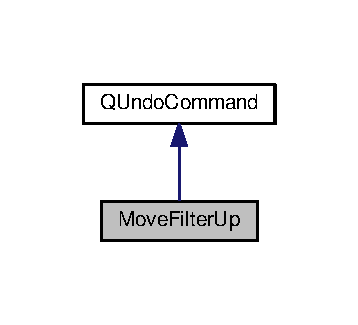
\includegraphics[width=172pt]{classUndoRedo_1_1MoveFilterUp__inherit__graph}
\end{center}
\end{figure}
\subsection*{Public Member Functions}
\begin{DoxyCompactItemize}
\item 
\hyperlink{classUndoRedo_1_1MoveFilterUp_ad11948fd1a203013d312b05633a01941}{Move\+Filter\+Up} (\hyperlink{classGUI_1_1FilterTab}{G\+U\+I\+::\+Filter\+Tab} $\ast$\hyperlink{classUndoRedo_1_1MoveFilterUp_a47ca82534a740774d79998759818d9f4}{filter\+Tab}, int old, int new\+\_\+1)
\item 
void \hyperlink{classUndoRedo_1_1MoveFilterUp_a0e1e7804a53f6d62efc72c9bdbec8571}{undo} ()
\item 
void \hyperlink{classUndoRedo_1_1MoveFilterUp_a93c48d6ed036e1a381be53ac67643284}{redo} ()
\end{DoxyCompactItemize}
\subsection*{Private Attributes}
\begin{DoxyCompactItemize}
\item 
int \hyperlink{classUndoRedo_1_1MoveFilterUp_aafdfcd92ee5fcb81a8ce268be0f53466}{old\+Index}
\item 
int \hyperlink{classUndoRedo_1_1MoveFilterUp_a12457b7d335917daf42dba277962d6b2}{new\+Index}
\item 
\hyperlink{classGUI_1_1FilterTab}{G\+U\+I\+::\+Filter\+Tab} $\ast$ \hyperlink{classUndoRedo_1_1MoveFilterUp_a47ca82534a740774d79998759818d9f4}{filter\+Tab}
\end{DoxyCompactItemize}


\subsection{Detailed Description}
This class is the undo command for moving a filter up in the filterlist. 

\subsection{Constructor \& Destructor Documentation}
\hypertarget{classUndoRedo_1_1MoveFilterUp_ad11948fd1a203013d312b05633a01941}{}\index{Undo\+Redo\+::\+Move\+Filter\+Up@{Undo\+Redo\+::\+Move\+Filter\+Up}!Move\+Filter\+Up@{Move\+Filter\+Up}}
\index{Move\+Filter\+Up@{Move\+Filter\+Up}!Undo\+Redo\+::\+Move\+Filter\+Up@{Undo\+Redo\+::\+Move\+Filter\+Up}}
\subsubsection[{Move\+Filter\+Up}]{\setlength{\rightskip}{0pt plus 5cm}{\bf Move\+Filter\+Up} (
\begin{DoxyParamCaption}
\item[{{\bf G\+U\+I\+::\+Filter\+Tab} $\ast$}]{filter\+Tab, }
\item[{int}]{old, }
\item[{int}]{new\+\_\+1}
\end{DoxyParamCaption}
)}\label{classUndoRedo_1_1MoveFilterUp_ad11948fd1a203013d312b05633a01941}


Constructor. 


\begin{DoxyParams}{Parameters}
{\em filter\+Tab} & The filtertab to operate on.\\
\hline
{\em old} & Old index of the filter.\\
\hline
{\em new} & New index of the filter.\\
\hline
\end{DoxyParams}


\subsection{Member Function Documentation}
\hypertarget{classUndoRedo_1_1MoveFilterUp_a93c48d6ed036e1a381be53ac67643284}{}\index{Undo\+Redo\+::\+Move\+Filter\+Up@{Undo\+Redo\+::\+Move\+Filter\+Up}!redo@{redo}}
\index{redo@{redo}!Undo\+Redo\+::\+Move\+Filter\+Up@{Undo\+Redo\+::\+Move\+Filter\+Up}}
\subsubsection[{redo}]{\setlength{\rightskip}{0pt plus 5cm}void redo (
\begin{DoxyParamCaption}
{}
\end{DoxyParamCaption}
)}\label{classUndoRedo_1_1MoveFilterUp_a93c48d6ed036e1a381be53ac67643284}


Moves selected filter one position up in the filterlist. 

\hypertarget{classUndoRedo_1_1MoveFilterUp_a0e1e7804a53f6d62efc72c9bdbec8571}{}\index{Undo\+Redo\+::\+Move\+Filter\+Up@{Undo\+Redo\+::\+Move\+Filter\+Up}!undo@{undo}}
\index{undo@{undo}!Undo\+Redo\+::\+Move\+Filter\+Up@{Undo\+Redo\+::\+Move\+Filter\+Up}}
\subsubsection[{undo}]{\setlength{\rightskip}{0pt plus 5cm}void undo (
\begin{DoxyParamCaption}
{}
\end{DoxyParamCaption}
)}\label{classUndoRedo_1_1MoveFilterUp_a0e1e7804a53f6d62efc72c9bdbec8571}


Moves the filter one position back down in the filterlist. 



\subsection{Field Documentation}
\hypertarget{classUndoRedo_1_1MoveFilterUp_a47ca82534a740774d79998759818d9f4}{}\index{Undo\+Redo\+::\+Move\+Filter\+Up@{Undo\+Redo\+::\+Move\+Filter\+Up}!filter\+Tab@{filter\+Tab}}
\index{filter\+Tab@{filter\+Tab}!Undo\+Redo\+::\+Move\+Filter\+Up@{Undo\+Redo\+::\+Move\+Filter\+Up}}
\subsubsection[{filter\+Tab}]{\setlength{\rightskip}{0pt plus 5cm}{\bf G\+U\+I\+::\+Filter\+Tab}$\ast$ filter\+Tab\hspace{0.3cm}{\ttfamily [private]}}\label{classUndoRedo_1_1MoveFilterUp_a47ca82534a740774d79998759818d9f4}
\hypertarget{classUndoRedo_1_1MoveFilterUp_a12457b7d335917daf42dba277962d6b2}{}\index{Undo\+Redo\+::\+Move\+Filter\+Up@{Undo\+Redo\+::\+Move\+Filter\+Up}!new\+Index@{new\+Index}}
\index{new\+Index@{new\+Index}!Undo\+Redo\+::\+Move\+Filter\+Up@{Undo\+Redo\+::\+Move\+Filter\+Up}}
\subsubsection[{new\+Index}]{\setlength{\rightskip}{0pt plus 5cm}int new\+Index\hspace{0.3cm}{\ttfamily [private]}}\label{classUndoRedo_1_1MoveFilterUp_a12457b7d335917daf42dba277962d6b2}
\hypertarget{classUndoRedo_1_1MoveFilterUp_aafdfcd92ee5fcb81a8ce268be0f53466}{}\index{Undo\+Redo\+::\+Move\+Filter\+Up@{Undo\+Redo\+::\+Move\+Filter\+Up}!old\+Index@{old\+Index}}
\index{old\+Index@{old\+Index}!Undo\+Redo\+::\+Move\+Filter\+Up@{Undo\+Redo\+::\+Move\+Filter\+Up}}
\subsubsection[{old\+Index}]{\setlength{\rightskip}{0pt plus 5cm}int old\+Index\hspace{0.3cm}{\ttfamily [private]}}\label{classUndoRedo_1_1MoveFilterUp_aafdfcd92ee5fcb81a8ce268be0f53466}

\newpage\hypertarget{classModel_1_1NegativeFilter}{}\section{Negative\+Filter Class Reference}
\label{classModel_1_1NegativeFilter}\index{Negative\+Filter@{Negative\+Filter}}


Inheritance diagram for Negative\+Filter\+:
\nopagebreak
\begin{figure}[H]
\begin{center}
\leavevmode
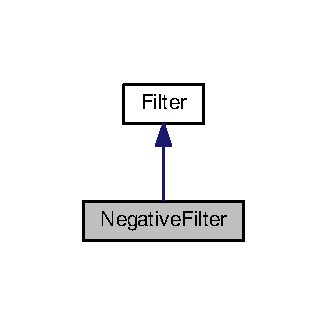
\includegraphics[width=157pt]{classModel_1_1NegativeFilter__inherit__graph}
\end{center}
\end{figure}
\subsection*{Public Member Functions}
\begin{DoxyCompactItemize}
\item 
\hyperlink{classModel_1_1NegativeFilter_ad17ab01ebb240c0211791ba615026351}{Negative\+Filter} ()
\item 
string \hyperlink{classModel_1_1NegativeFilter_a62b7b60e24f92234393b840b35808e06}{get\+Filter\+Description} ()
\item 
string \hyperlink{classModel_1_1NegativeFilter_a11335e13e50af74108bf926dc1340b4b}{get\+Name} ()
\end{DoxyCompactItemize}
\subsection*{Additional Inherited Members}


\subsection{Detailed Description}
Converts the video into it\textquotesingle{}s negative. 

\subsection{Constructor \& Destructor Documentation}
\hypertarget{classModel_1_1NegativeFilter_ad17ab01ebb240c0211791ba615026351}{}\index{Model\+::\+Negative\+Filter@{Model\+::\+Negative\+Filter}!Negative\+Filter@{Negative\+Filter}}
\index{Negative\+Filter@{Negative\+Filter}!Model\+::\+Negative\+Filter@{Model\+::\+Negative\+Filter}}
\subsubsection[{Negative\+Filter}]{\setlength{\rightskip}{0pt plus 5cm}{\bf Negative\+Filter} (
\begin{DoxyParamCaption}
{}
\end{DoxyParamCaption}
)}\label{classModel_1_1NegativeFilter_ad17ab01ebb240c0211791ba615026351}


Constructor. 



\subsection{Member Function Documentation}
\hypertarget{classModel_1_1NegativeFilter_a62b7b60e24f92234393b840b35808e06}{}\index{Model\+::\+Negative\+Filter@{Model\+::\+Negative\+Filter}!get\+Filter\+Description@{get\+Filter\+Description}}
\index{get\+Filter\+Description@{get\+Filter\+Description}!Model\+::\+Negative\+Filter@{Model\+::\+Negative\+Filter}}
\subsubsection[{get\+Filter\+Description}]{\setlength{\rightskip}{0pt plus 5cm}string get\+Filter\+Description (
\begin{DoxyParamCaption}
{}
\end{DoxyParamCaption}
)\hspace{0.3cm}{\ttfamily [virtual]}}\label{classModel_1_1NegativeFilter_a62b7b60e24f92234393b840b35808e06}


Returns the string that the ffmpeg library needs to apply the filter to a video. 

\begin{DoxyReturn}{Returns}
The string for the ffmpeg library.
\end{DoxyReturn}


Implements \hyperlink{classModel_1_1Filter_a453fcafa809afa1ce58d9ef95d5f26c0}{Filter}.

\hypertarget{classModel_1_1NegativeFilter_a11335e13e50af74108bf926dc1340b4b}{}\index{Model\+::\+Negative\+Filter@{Model\+::\+Negative\+Filter}!get\+Name@{get\+Name}}
\index{get\+Name@{get\+Name}!Model\+::\+Negative\+Filter@{Model\+::\+Negative\+Filter}}
\subsubsection[{get\+Name}]{\setlength{\rightskip}{0pt plus 5cm}string get\+Name (
\begin{DoxyParamCaption}
{}
\end{DoxyParamCaption}
)\hspace{0.3cm}{\ttfamily [virtual]}}\label{classModel_1_1NegativeFilter_a11335e13e50af74108bf926dc1340b4b}


Returns the name of the filter. 

\begin{DoxyReturn}{Returns}
The filtername.
\end{DoxyReturn}


Implements \hyperlink{classModel_1_1Filter_ade93aa98c68d185a9c03784d36140225}{Filter}.


\newpage\hypertarget{classModel_1_1NoiseFilter}{}\section{Noise\+Filter Class Reference}
\label{classModel_1_1NoiseFilter}\index{Noise\+Filter@{Noise\+Filter}}


Inheritance diagram for Noise\+Filter\+:
\nopagebreak
\begin{figure}[H]
\begin{center}
\leavevmode
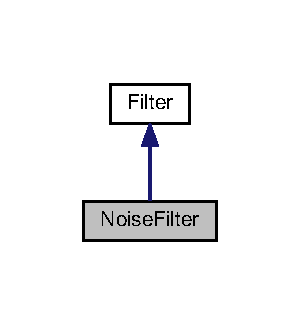
\includegraphics[width=144pt]{classModel_1_1NoiseFilter__inherit__graph}
\end{center}
\end{figure}
\subsection*{Public Member Functions}
\begin{DoxyCompactItemize}
\item 
\hyperlink{classModel_1_1NoiseFilter_ae0fddd4ce827a9428beb93c8fd39ea6a}{Noise\+Filter} ()
\item 
string \hyperlink{classModel_1_1NoiseFilter_a62b7b60e24f92234393b840b35808e06}{get\+Filter\+Description} ()
\item 
\hyperlink{namespaceModel_a0466e3095e9c21e5864d8964e9d7df59}{Model\+::\+Noise\+Mode} \hyperlink{classModel_1_1NoiseFilter_ab7a70a6b1910334e61531f5b65a4fa9a}{get\+Mode} ()
\item 
void \hyperlink{classModel_1_1NoiseFilter_acee86eb98b73f986b5e37610f6c3ab9c}{set\+Mode} (\hyperlink{namespaceModel_a0466e3095e9c21e5864d8964e9d7df59}{Model\+::\+Noise\+Mode} \hyperlink{classModel_1_1NoiseFilter_a0c65c7ea38f862aa144334b677f07a7c}{mode})
\item 
int \hyperlink{classModel_1_1NoiseFilter_a708995fb1b6acb31ee0dfb0f4881e5b5}{get\+Intensity} ()
\item 
string \hyperlink{classModel_1_1NoiseFilter_a11335e13e50af74108bf926dc1340b4b}{get\+Name} ()
\item 
void \hyperlink{classModel_1_1NoiseFilter_ac8255ffbc46bb61acaa8fd23d0d260eb}{set\+Intensity} (int \hyperlink{classModel_1_1NoiseFilter_a299ec0c42ccc5a2d79d1739428ac3210}{intensity})
\end{DoxyCompactItemize}
\subsection*{Private Attributes}
\begin{DoxyCompactItemize}
\item 
int \hyperlink{classModel_1_1NoiseFilter_a299ec0c42ccc5a2d79d1739428ac3210}{intensity}
\item 
\hyperlink{namespaceModel_a0466e3095e9c21e5864d8964e9d7df59}{Model\+::\+Noise\+Mode} $\ast$ \hyperlink{classModel_1_1NoiseFilter_a0c65c7ea38f862aa144334b677f07a7c}{mode}
\end{DoxyCompactItemize}
\subsection*{Additional Inherited Members}


\subsection{Detailed Description}
Inserts noise into the video. 

\subsection{Constructor \& Destructor Documentation}
\hypertarget{classModel_1_1NoiseFilter_ae0fddd4ce827a9428beb93c8fd39ea6a}{}\index{Model\+::\+Noise\+Filter@{Model\+::\+Noise\+Filter}!Noise\+Filter@{Noise\+Filter}}
\index{Noise\+Filter@{Noise\+Filter}!Model\+::\+Noise\+Filter@{Model\+::\+Noise\+Filter}}
\subsubsection[{Noise\+Filter}]{\setlength{\rightskip}{0pt plus 5cm}{\bf Noise\+Filter} (
\begin{DoxyParamCaption}
{}
\end{DoxyParamCaption}
)}\label{classModel_1_1NoiseFilter_ae0fddd4ce827a9428beb93c8fd39ea6a}


Constructor. 



\subsection{Member Function Documentation}
\hypertarget{classModel_1_1NoiseFilter_a62b7b60e24f92234393b840b35808e06}{}\index{Model\+::\+Noise\+Filter@{Model\+::\+Noise\+Filter}!get\+Filter\+Description@{get\+Filter\+Description}}
\index{get\+Filter\+Description@{get\+Filter\+Description}!Model\+::\+Noise\+Filter@{Model\+::\+Noise\+Filter}}
\subsubsection[{get\+Filter\+Description}]{\setlength{\rightskip}{0pt plus 5cm}string get\+Filter\+Description (
\begin{DoxyParamCaption}
{}
\end{DoxyParamCaption}
)\hspace{0.3cm}{\ttfamily [virtual]}}\label{classModel_1_1NoiseFilter_a62b7b60e24f92234393b840b35808e06}


Returns the string that the ffmpeg library needs to apply the filter to a video. 

\begin{DoxyReturn}{Returns}
The string for the ffmpeg library.
\end{DoxyReturn}


Implements \hyperlink{classModel_1_1Filter_a453fcafa809afa1ce58d9ef95d5f26c0}{Filter}.

\hypertarget{classModel_1_1NoiseFilter_a708995fb1b6acb31ee0dfb0f4881e5b5}{}\index{Model\+::\+Noise\+Filter@{Model\+::\+Noise\+Filter}!get\+Intensity@{get\+Intensity}}
\index{get\+Intensity@{get\+Intensity}!Model\+::\+Noise\+Filter@{Model\+::\+Noise\+Filter}}
\subsubsection[{get\+Intensity}]{\setlength{\rightskip}{0pt plus 5cm}int get\+Intensity (
\begin{DoxyParamCaption}
{}
\end{DoxyParamCaption}
)}\label{classModel_1_1NoiseFilter_a708995fb1b6acb31ee0dfb0f4881e5b5}


Returns the intensity of the noise. 

\begin{DoxyReturn}{Returns}
The noise intensity.
\end{DoxyReturn}
\hypertarget{classModel_1_1NoiseFilter_ab7a70a6b1910334e61531f5b65a4fa9a}{}\index{Model\+::\+Noise\+Filter@{Model\+::\+Noise\+Filter}!get\+Mode@{get\+Mode}}
\index{get\+Mode@{get\+Mode}!Model\+::\+Noise\+Filter@{Model\+::\+Noise\+Filter}}
\subsubsection[{get\+Mode}]{\setlength{\rightskip}{0pt plus 5cm}{\bf Model\+::\+Noise\+Mode} get\+Mode (
\begin{DoxyParamCaption}
{}
\end{DoxyParamCaption}
)}\label{classModel_1_1NoiseFilter_ab7a70a6b1910334e61531f5b65a4fa9a}


Returns the Noise\+Mode. 

\begin{DoxyReturn}{Returns}
The Noise\+Mode.
\end{DoxyReturn}
\hypertarget{classModel_1_1NoiseFilter_a11335e13e50af74108bf926dc1340b4b}{}\index{Model\+::\+Noise\+Filter@{Model\+::\+Noise\+Filter}!get\+Name@{get\+Name}}
\index{get\+Name@{get\+Name}!Model\+::\+Noise\+Filter@{Model\+::\+Noise\+Filter}}
\subsubsection[{get\+Name}]{\setlength{\rightskip}{0pt plus 5cm}string get\+Name (
\begin{DoxyParamCaption}
{}
\end{DoxyParamCaption}
)\hspace{0.3cm}{\ttfamily [virtual]}}\label{classModel_1_1NoiseFilter_a11335e13e50af74108bf926dc1340b4b}


Returns the name of the filter. 

\begin{DoxyReturn}{Returns}
The filtername.
\end{DoxyReturn}


Implements \hyperlink{classModel_1_1Filter_ade93aa98c68d185a9c03784d36140225}{Filter}.

\hypertarget{classModel_1_1NoiseFilter_ac8255ffbc46bb61acaa8fd23d0d260eb}{}\index{Model\+::\+Noise\+Filter@{Model\+::\+Noise\+Filter}!set\+Intensity@{set\+Intensity}}
\index{set\+Intensity@{set\+Intensity}!Model\+::\+Noise\+Filter@{Model\+::\+Noise\+Filter}}
\subsubsection[{set\+Intensity}]{\setlength{\rightskip}{0pt plus 5cm}void set\+Intensity (
\begin{DoxyParamCaption}
\item[{int}]{intensity}
\end{DoxyParamCaption}
)}\label{classModel_1_1NoiseFilter_ac8255ffbc46bb61acaa8fd23d0d260eb}


Sets the intensity of the noise. 


\begin{DoxyParams}{Parameters}
{\em intensity} & The new intensity of the noise.\\
\hline
\end{DoxyParams}
\hypertarget{classModel_1_1NoiseFilter_acee86eb98b73f986b5e37610f6c3ab9c}{}\index{Model\+::\+Noise\+Filter@{Model\+::\+Noise\+Filter}!set\+Mode@{set\+Mode}}
\index{set\+Mode@{set\+Mode}!Model\+::\+Noise\+Filter@{Model\+::\+Noise\+Filter}}
\subsubsection[{set\+Mode}]{\setlength{\rightskip}{0pt plus 5cm}void set\+Mode (
\begin{DoxyParamCaption}
\item[{{\bf Model\+::\+Noise\+Mode}}]{mode}
\end{DoxyParamCaption}
)}\label{classModel_1_1NoiseFilter_acee86eb98b73f986b5e37610f6c3ab9c}


Sets the Noise\+Mode. 


\begin{DoxyParams}{Parameters}
{\em mode} & The new Noise\+Mode.\\
\hline
\end{DoxyParams}


\subsection{Field Documentation}
\hypertarget{classModel_1_1NoiseFilter_a299ec0c42ccc5a2d79d1739428ac3210}{}\index{Model\+::\+Noise\+Filter@{Model\+::\+Noise\+Filter}!intensity@{intensity}}
\index{intensity@{intensity}!Model\+::\+Noise\+Filter@{Model\+::\+Noise\+Filter}}
\subsubsection[{intensity}]{\setlength{\rightskip}{0pt plus 5cm}int intensity\hspace{0.3cm}{\ttfamily [private]}}\label{classModel_1_1NoiseFilter_a299ec0c42ccc5a2d79d1739428ac3210}
\hypertarget{classModel_1_1NoiseFilter_a0c65c7ea38f862aa144334b677f07a7c}{}\index{Model\+::\+Noise\+Filter@{Model\+::\+Noise\+Filter}!mode@{mode}}
\index{mode@{mode}!Model\+::\+Noise\+Filter@{Model\+::\+Noise\+Filter}}
\subsubsection[{mode}]{\setlength{\rightskip}{0pt plus 5cm}{\bf Model\+::\+Noise\+Mode}$\ast$ mode\hspace{0.3cm}{\ttfamily [private]}}\label{classModel_1_1NoiseFilter_a0c65c7ea38f862aa144334b677f07a7c}

\newpage\hypertarget{classGUI_1_1NoiseFilterBox}{}\section{Noise\+Filter\+Box Class Reference}
\label{classGUI_1_1NoiseFilterBox}\index{Noise\+Filter\+Box@{Noise\+Filter\+Box}}
\subsection*{Public Member Functions}
\begin{DoxyCompactItemize}
\item 
\hypertarget{classGUI_1_1NoiseFilterBox_ad72bee39e6bcf5b241523aee68cb84c1}{}{\bfseries Noise\+Filter\+Box} (\hyperlink{classGUI_1_1QtGui_1_1QWidget____10}{G\+U\+I\+::\+Qt\+Gui\+::\+Q\+Widget\+\_\+\+\_\+10} $\ast$parent)\label{classGUI_1_1NoiseFilterBox_ad72bee39e6bcf5b241523aee68cb84c1}

\item 
\hypertarget{classGUI_1_1NoiseFilterBox_ad7c0ee00fe3faac7942d75eec2a5342b}{}virtual void {\bfseries set\+Filter} (\hyperlink{classModel_1_1Filter_1_1Filter}{Model\+::\+Filter\+::\+Filter} \&filter)\label{classGUI_1_1NoiseFilterBox_ad7c0ee00fe3faac7942d75eec2a5342b}

\item 
\hypertarget{classGUI_1_1NoiseFilterBox_acef2029a93f4ab3a538cdb643b9c2613}{}virtual \hyperlink{classModel_1_1Filter_1_1Filter}{Model\+::\+Filter\+::\+Filter} $\ast$ {\bfseries get\+Filter} ()\label{classGUI_1_1NoiseFilterBox_acef2029a93f4ab3a538cdb643b9c2613}

\end{DoxyCompactItemize}

\newpage\hypertarget{classGUI_1_1PlainFilterBox}{}\section{Plain\+Filter\+Box Class Reference}
\label{classGUI_1_1PlainFilterBox}\index{Plain\+Filter\+Box@{Plain\+Filter\+Box}}


Inheritance diagram for Plain\+Filter\+Box\+:
\nopagebreak
\begin{figure}[H]
\begin{center}
\leavevmode
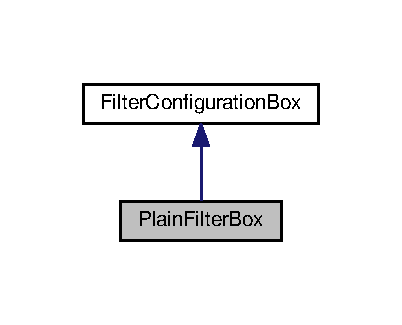
\includegraphics[width=193pt]{classGUI_1_1PlainFilterBox__inherit__graph}
\end{center}
\end{figure}
\subsection*{Public Member Functions}
\begin{DoxyCompactItemize}
\item 
\hyperlink{classGUI_1_1PlainFilterBox_aa1ea3acc7f77156212b9a17905626a9a}{Plain\+Filter\+Box} (\hyperlink{classGUI_1_1QWidget}{G\+U\+I\+::\+Q\+Widget} $\ast$parent)
\end{DoxyCompactItemize}
\subsection*{Additional Inherited Members}


\subsection{Detailed Description}
This class contains no sliders to adjust filter options. 

\subsection{Constructor \& Destructor Documentation}
\hypertarget{classGUI_1_1PlainFilterBox_aa1ea3acc7f77156212b9a17905626a9a}{}\index{G\+U\+I\+::\+Plain\+Filter\+Box@{G\+U\+I\+::\+Plain\+Filter\+Box}!Plain\+Filter\+Box@{Plain\+Filter\+Box}}
\index{Plain\+Filter\+Box@{Plain\+Filter\+Box}!G\+U\+I\+::\+Plain\+Filter\+Box@{G\+U\+I\+::\+Plain\+Filter\+Box}}
\subsubsection[{Plain\+Filter\+Box}]{\setlength{\rightskip}{0pt plus 5cm}{\bf Plain\+Filter\+Box} (
\begin{DoxyParamCaption}
\item[{{\bf G\+U\+I\+::\+Q\+Widget} $\ast$}]{parent}
\end{DoxyParamCaption}
)}\label{classGUI_1_1PlainFilterBox_aa1ea3acc7f77156212b9a17905626a9a}


Constructor. 


\newpage\hypertarget{classGUI_1_1Player}{}\section{Player Class Reference}
\label{classGUI_1_1Player}\index{Player@{Player}}


Inheritance diagram for Player\+:
\nopagebreak
\begin{figure}[H]
\begin{center}
\leavevmode
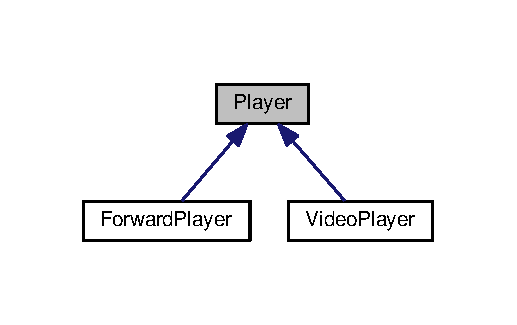
\includegraphics[width=248pt]{classGUI_1_1Player__inherit__graph}
\end{center}
\end{figure}
\subsection*{Public Member Functions}
\begin{DoxyCompactItemize}
\item 
virtual void \hyperlink{classGUI_1_1Player_aa3c4df4568ad2126665a07db4e1f59b6}{play} ()=0
\item 
virtual void \hyperlink{classGUI_1_1Player_a0edeed26c37624e7aa90f391c9a7128f}{pause} ()=0
\item 
virtual void \hyperlink{classGUI_1_1Player_a7a0e5d7c45657ca21b5b8d0d4b0a0e7b}{stop} ()=0
\item 
virtual void \hyperlink{classGUI_1_1Player_af64b0827c381fcd751fe2bbbf38682f4}{next\+Frame} ()=0
\item 
virtual void \hyperlink{classGUI_1_1Player_a4db6c8b8c8e9b567d466181337cdc001}{previous\+Frame} ()=0
\item 
virtual void \hyperlink{classGUI_1_1Player_a1c7d2ab9f6c21f2e7bf15a2ec9841a0a}{set\+Speed} (float speed)=0
\item 
virtual void \hyperlink{classGUI_1_1Player_acf5fb178b5d9a7f5f4bd198a13ae6bf7}{set\+Position} (int position)=0
\item 
virtual int \hyperlink{classGUI_1_1Player_a889dbfa5524d69dcc31d377d2d9bd230}{get\+Position} ()=0
\item 
virtual float \hyperlink{classGUI_1_1Player_a349fa93e666bd9fb256a238a3194f948}{get\+Speed} ()=0
\item 
virtual bool \hyperlink{classGUI_1_1Player_a4fbad8972dd248e6c8f5dc2c898a9bc7}{is\+Playing} ()=0
\item 
virtual bool \hyperlink{classGUI_1_1Player_ab9e7bd794ed42cea965c5250ec804225}{is\+Stopped} ()=0
\item 
virtual void \hyperlink{classGUI_1_1Player_a00af5c2c5e03cb5748a94d936fe34d9a}{reset} ()=0
\end{DoxyCompactItemize}
\subsection*{Data Fields}
\begin{DoxyCompactItemize}
\item 
\hyperlink{classGUI_1_1ControlPanel}{G\+U\+I\+::\+Control\+Panel} $\ast$ \hyperlink{classGUI_1_1Player_a068c1591fd22d057fcaf36617c45d557}{players}
\item 
\hyperlink{classGUI_1_1ControlPanel}{G\+U\+I\+::\+Control\+Panel} $\ast$ \hyperlink{classGUI_1_1Player_a3c9f4437b3e54e8bd9ad90739f051abc}{master\+Player}
\end{DoxyCompactItemize}


\subsection{Detailed Description}
This class is the base class for players. 

\subsection{Member Function Documentation}
\hypertarget{classGUI_1_1Player_a889dbfa5524d69dcc31d377d2d9bd230}{}\index{G\+U\+I\+::\+Player@{G\+U\+I\+::\+Player}!get\+Position@{get\+Position}}
\index{get\+Position@{get\+Position}!G\+U\+I\+::\+Player@{G\+U\+I\+::\+Player}}
\subsubsection[{get\+Position}]{\setlength{\rightskip}{0pt plus 5cm}int get\+Position (
\begin{DoxyParamCaption}
{}
\end{DoxyParamCaption}
)\hspace{0.3cm}{\ttfamily [pure virtual]}}\label{classGUI_1_1Player_a889dbfa5524d69dcc31d377d2d9bd230}


Returns the position in the video. 

\begin{DoxyReturn}{Returns}
The current position.
\end{DoxyReturn}


Implemented in \hyperlink{classGUI_1_1VideoPlayer_a97825791568ee242ca19d25b75030d87}{Video\+Player}, and \hyperlink{classGUI_1_1ForwardPlayer_a97825791568ee242ca19d25b75030d87}{Forward\+Player}.

\hypertarget{classGUI_1_1Player_a349fa93e666bd9fb256a238a3194f948}{}\index{G\+U\+I\+::\+Player@{G\+U\+I\+::\+Player}!get\+Speed@{get\+Speed}}
\index{get\+Speed@{get\+Speed}!G\+U\+I\+::\+Player@{G\+U\+I\+::\+Player}}
\subsubsection[{get\+Speed}]{\setlength{\rightskip}{0pt plus 5cm}float get\+Speed (
\begin{DoxyParamCaption}
{}
\end{DoxyParamCaption}
)\hspace{0.3cm}{\ttfamily [pure virtual]}}\label{classGUI_1_1Player_a349fa93e666bd9fb256a238a3194f948}


Returns the speed. 

\begin{DoxyReturn}{Returns}
The current speed.
\end{DoxyReturn}


Implemented in \hyperlink{classGUI_1_1VideoPlayer_a26ebefde7fe71954e6c1282255951b7d}{Video\+Player}, and \hyperlink{classGUI_1_1ForwardPlayer_a26ebefde7fe71954e6c1282255951b7d}{Forward\+Player}.

\hypertarget{classGUI_1_1Player_a4fbad8972dd248e6c8f5dc2c898a9bc7}{}\index{G\+U\+I\+::\+Player@{G\+U\+I\+::\+Player}!is\+Playing@{is\+Playing}}
\index{is\+Playing@{is\+Playing}!G\+U\+I\+::\+Player@{G\+U\+I\+::\+Player}}
\subsubsection[{is\+Playing}]{\setlength{\rightskip}{0pt plus 5cm}bool is\+Playing (
\begin{DoxyParamCaption}
{}
\end{DoxyParamCaption}
)\hspace{0.3cm}{\ttfamily [pure virtual]}}\label{classGUI_1_1Player_a4fbad8972dd248e6c8f5dc2c898a9bc7}


Whether the player is currently playing. 

\begin{DoxyReturn}{Returns}
True if the player is playing.
\end{DoxyReturn}


Implemented in \hyperlink{classGUI_1_1VideoPlayer_a8438e3403946accc1986a05b89ee7b03}{Video\+Player}, and \hyperlink{classGUI_1_1ForwardPlayer_a8438e3403946accc1986a05b89ee7b03}{Forward\+Player}.

\hypertarget{classGUI_1_1Player_ab9e7bd794ed42cea965c5250ec804225}{}\index{G\+U\+I\+::\+Player@{G\+U\+I\+::\+Player}!is\+Stopped@{is\+Stopped}}
\index{is\+Stopped@{is\+Stopped}!G\+U\+I\+::\+Player@{G\+U\+I\+::\+Player}}
\subsubsection[{is\+Stopped}]{\setlength{\rightskip}{0pt plus 5cm}bool is\+Stopped (
\begin{DoxyParamCaption}
{}
\end{DoxyParamCaption}
)\hspace{0.3cm}{\ttfamily [pure virtual]}}\label{classGUI_1_1Player_ab9e7bd794ed42cea965c5250ec804225}


Whether the player is stopped. 

\begin{DoxyReturn}{Returns}
True if the player is stopped.
\end{DoxyReturn}


Implemented in \hyperlink{classGUI_1_1VideoPlayer_a2fc5ff4f369aaa46c55c3ad3c63216d6}{Video\+Player}, and \hyperlink{classGUI_1_1ForwardPlayer_a2fc5ff4f369aaa46c55c3ad3c63216d6}{Forward\+Player}.

\hypertarget{classGUI_1_1Player_af64b0827c381fcd751fe2bbbf38682f4}{}\index{G\+U\+I\+::\+Player@{G\+U\+I\+::\+Player}!next\+Frame@{next\+Frame}}
\index{next\+Frame@{next\+Frame}!G\+U\+I\+::\+Player@{G\+U\+I\+::\+Player}}
\subsubsection[{next\+Frame}]{\setlength{\rightskip}{0pt plus 5cm}void next\+Frame (
\begin{DoxyParamCaption}
{}
\end{DoxyParamCaption}
)\hspace{0.3cm}{\ttfamily [pure virtual]}}\label{classGUI_1_1Player_af64b0827c381fcd751fe2bbbf38682f4}


Shows the next frame. 



Implemented in \hyperlink{classGUI_1_1VideoPlayer_a365329da56f8b07f8c95027ba967bbc3}{Video\+Player}, and \hyperlink{classGUI_1_1ForwardPlayer_a365329da56f8b07f8c95027ba967bbc3}{Forward\+Player}.

\hypertarget{classGUI_1_1Player_a0edeed26c37624e7aa90f391c9a7128f}{}\index{G\+U\+I\+::\+Player@{G\+U\+I\+::\+Player}!pause@{pause}}
\index{pause@{pause}!G\+U\+I\+::\+Player@{G\+U\+I\+::\+Player}}
\subsubsection[{pause}]{\setlength{\rightskip}{0pt plus 5cm}void pause (
\begin{DoxyParamCaption}
{}
\end{DoxyParamCaption}
)\hspace{0.3cm}{\ttfamily [pure virtual]}}\label{classGUI_1_1Player_a0edeed26c37624e7aa90f391c9a7128f}


Pauses the video. 



Implemented in \hyperlink{classGUI_1_1VideoPlayer_a7167f5c196fc5e167bfabde1a730e81d}{Video\+Player}, and \hyperlink{classGUI_1_1ForwardPlayer_a7167f5c196fc5e167bfabde1a730e81d}{Forward\+Player}.

\hypertarget{classGUI_1_1Player_aa3c4df4568ad2126665a07db4e1f59b6}{}\index{G\+U\+I\+::\+Player@{G\+U\+I\+::\+Player}!play@{play}}
\index{play@{play}!G\+U\+I\+::\+Player@{G\+U\+I\+::\+Player}}
\subsubsection[{play}]{\setlength{\rightskip}{0pt plus 5cm}void play (
\begin{DoxyParamCaption}
{}
\end{DoxyParamCaption}
)\hspace{0.3cm}{\ttfamily [pure virtual]}}\label{classGUI_1_1Player_aa3c4df4568ad2126665a07db4e1f59b6}


Plays the video. 



Implemented in \hyperlink{classGUI_1_1VideoPlayer_a6d58098c6cf63c241ed03bc797256bb1}{Video\+Player}, and \hyperlink{classGUI_1_1ForwardPlayer_a6d58098c6cf63c241ed03bc797256bb1}{Forward\+Player}.

\hypertarget{classGUI_1_1Player_a4db6c8b8c8e9b567d466181337cdc001}{}\index{G\+U\+I\+::\+Player@{G\+U\+I\+::\+Player}!previous\+Frame@{previous\+Frame}}
\index{previous\+Frame@{previous\+Frame}!G\+U\+I\+::\+Player@{G\+U\+I\+::\+Player}}
\subsubsection[{previous\+Frame}]{\setlength{\rightskip}{0pt plus 5cm}void previous\+Frame (
\begin{DoxyParamCaption}
{}
\end{DoxyParamCaption}
)\hspace{0.3cm}{\ttfamily [pure virtual]}}\label{classGUI_1_1Player_a4db6c8b8c8e9b567d466181337cdc001}


Shows the previous frame. 



Implemented in \hyperlink{classGUI_1_1VideoPlayer_a3c96ed37c70ebc0b32c527a04e1536d1}{Video\+Player}, and \hyperlink{classGUI_1_1ForwardPlayer_a3c96ed37c70ebc0b32c527a04e1536d1}{Forward\+Player}.

\hypertarget{classGUI_1_1Player_a00af5c2c5e03cb5748a94d936fe34d9a}{}\index{G\+U\+I\+::\+Player@{G\+U\+I\+::\+Player}!reset@{reset}}
\index{reset@{reset}!G\+U\+I\+::\+Player@{G\+U\+I\+::\+Player}}
\subsubsection[{reset}]{\setlength{\rightskip}{0pt plus 5cm}void reset (
\begin{DoxyParamCaption}
{}
\end{DoxyParamCaption}
)\hspace{0.3cm}{\ttfamily [pure virtual]}}\label{classGUI_1_1Player_a00af5c2c5e03cb5748a94d936fe34d9a}


Resets the player. 



Implemented in \hyperlink{classGUI_1_1VideoPlayer_ad20897c5c8bd47f5d4005989bead0e55}{Video\+Player}, and \hyperlink{classGUI_1_1ForwardPlayer_ad20897c5c8bd47f5d4005989bead0e55}{Forward\+Player}.

\hypertarget{classGUI_1_1Player_acf5fb178b5d9a7f5f4bd198a13ae6bf7}{}\index{G\+U\+I\+::\+Player@{G\+U\+I\+::\+Player}!set\+Position@{set\+Position}}
\index{set\+Position@{set\+Position}!G\+U\+I\+::\+Player@{G\+U\+I\+::\+Player}}
\subsubsection[{set\+Position}]{\setlength{\rightskip}{0pt plus 5cm}void set\+Position (
\begin{DoxyParamCaption}
\item[{int}]{position}
\end{DoxyParamCaption}
)\hspace{0.3cm}{\ttfamily [pure virtual]}}\label{classGUI_1_1Player_acf5fb178b5d9a7f5f4bd198a13ae6bf7}


Sets the position in the video. 


\begin{DoxyParams}{Parameters}
{\em position} & The new position.\\
\hline
\end{DoxyParams}


Implemented in \hyperlink{classGUI_1_1VideoPlayer_a1aa68f77243229daea38d59bc5145d35}{Video\+Player}, and \hyperlink{classGUI_1_1ForwardPlayer_a1aa68f77243229daea38d59bc5145d35}{Forward\+Player}.

\hypertarget{classGUI_1_1Player_a1c7d2ab9f6c21f2e7bf15a2ec9841a0a}{}\index{G\+U\+I\+::\+Player@{G\+U\+I\+::\+Player}!set\+Speed@{set\+Speed}}
\index{set\+Speed@{set\+Speed}!G\+U\+I\+::\+Player@{G\+U\+I\+::\+Player}}
\subsubsection[{set\+Speed}]{\setlength{\rightskip}{0pt plus 5cm}void set\+Speed (
\begin{DoxyParamCaption}
\item[{float}]{speed}
\end{DoxyParamCaption}
)\hspace{0.3cm}{\ttfamily [pure virtual]}}\label{classGUI_1_1Player_a1c7d2ab9f6c21f2e7bf15a2ec9841a0a}


Sets the speed. 


\begin{DoxyParams}{Parameters}
{\em speed} & The new speed.\\
\hline
\end{DoxyParams}


Implemented in \hyperlink{classGUI_1_1VideoPlayer_a5466c67c5ec22359c0702dc4ac8ffb19}{Video\+Player}, and \hyperlink{classGUI_1_1ForwardPlayer_a5466c67c5ec22359c0702dc4ac8ffb19}{Forward\+Player}.

\hypertarget{classGUI_1_1Player_a7a0e5d7c45657ca21b5b8d0d4b0a0e7b}{}\index{G\+U\+I\+::\+Player@{G\+U\+I\+::\+Player}!stop@{stop}}
\index{stop@{stop}!G\+U\+I\+::\+Player@{G\+U\+I\+::\+Player}}
\subsubsection[{stop}]{\setlength{\rightskip}{0pt plus 5cm}void stop (
\begin{DoxyParamCaption}
{}
\end{DoxyParamCaption}
)\hspace{0.3cm}{\ttfamily [pure virtual]}}\label{classGUI_1_1Player_a7a0e5d7c45657ca21b5b8d0d4b0a0e7b}


Stops the video. 



Implemented in \hyperlink{classGUI_1_1VideoPlayer_a8c528baf37154d347366083f0f816846}{Video\+Player}, and \hyperlink{classGUI_1_1ForwardPlayer_a8c528baf37154d347366083f0f816846}{Forward\+Player}.



\subsection{Field Documentation}
\hypertarget{classGUI_1_1Player_a3c9f4437b3e54e8bd9ad90739f051abc}{}\index{G\+U\+I\+::\+Player@{G\+U\+I\+::\+Player}!master\+Player@{master\+Player}}
\index{master\+Player@{master\+Player}!G\+U\+I\+::\+Player@{G\+U\+I\+::\+Player}}
\subsubsection[{master\+Player}]{\setlength{\rightskip}{0pt plus 5cm}{\bf G\+U\+I\+::\+Control\+Panel}$\ast$ master\+Player}\label{classGUI_1_1Player_a3c9f4437b3e54e8bd9ad90739f051abc}
\hypertarget{classGUI_1_1Player_a068c1591fd22d057fcaf36617c45d557}{}\index{G\+U\+I\+::\+Player@{G\+U\+I\+::\+Player}!players@{players}}
\index{players@{players}!G\+U\+I\+::\+Player@{G\+U\+I\+::\+Player}}
\subsubsection[{players}]{\setlength{\rightskip}{0pt plus 5cm}{\bf G\+U\+I\+::\+Control\+Panel}$\ast$ players}\label{classGUI_1_1Player_a068c1591fd22d057fcaf36617c45d557}

\newpage\hypertarget{classGUI_1_1PlayerControlPanel}{}\section{Player\+Control\+Panel Class Reference}
\label{classGUI_1_1PlayerControlPanel}\index{Player\+Control\+Panel@{Player\+Control\+Panel}}


Inheritance diagram for Player\+Control\+Panel\+:
\nopagebreak
\begin{figure}[H]
\begin{center}
\leavevmode
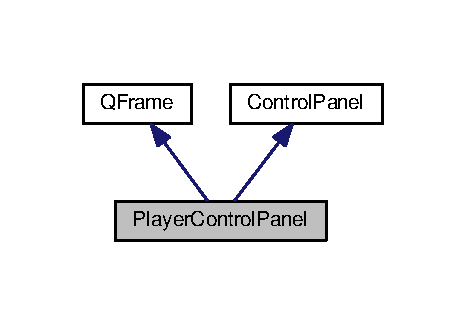
\includegraphics[width=224pt]{classGUI_1_1PlayerControlPanel__inherit__graph}
\end{center}
\end{figure}
\subsection*{Public Member Functions}
\begin{DoxyCompactItemize}
\item 
\hyperlink{classGUI_1_1PlayerControlPanel_a0432cd20dc9d144a23a8f8323fd68022}{Player\+Control\+Panel} (\hyperlink{classGUI_1_1QWidget}{Q\+Widget} $\ast$parent=0)
\item 
void \hyperlink{classGUI_1_1PlayerControlPanel_ae13c7f95f1ceda0fec18d18c3d7619f6}{update\+Ui} ()
\end{DoxyCompactItemize}
\subsection*{Private Member Functions}
\begin{DoxyCompactItemize}
\item 
void \hyperlink{classGUI_1_1PlayerControlPanel_aa72182c9a958af0e87b65ab7bdba0035}{create\+Ui} ()
\item 
void \hyperlink{classGUI_1_1PlayerControlPanel_a5176c9496a29e21eacb0f81ca1a29923}{create\+Actions} ()
\item 
void \hyperlink{classGUI_1_1PlayerControlPanel_a6d58098c6cf63c241ed03bc797256bb1}{play} ()
\item 
void \hyperlink{classGUI_1_1PlayerControlPanel_a7167f5c196fc5e167bfabde1a730e81d}{pause} ()
\item 
void \hyperlink{classGUI_1_1PlayerControlPanel_a8c528baf37154d347366083f0f816846}{stop} ()
\item 
void \hyperlink{classGUI_1_1PlayerControlPanel_a365329da56f8b07f8c95027ba967bbc3}{next\+Frame} ()
\item 
void \hyperlink{classGUI_1_1PlayerControlPanel_a3c96ed37c70ebc0b32c527a04e1536d1}{previous\+Frame} ()
\item 
void \hyperlink{classGUI_1_1PlayerControlPanel_a5589e2287b95a33fb20081ea7332e9bf}{change\+Speed} (int index)
\item 
void \hyperlink{classGUI_1_1PlayerControlPanel_a8941b919cc55ba59b57f9d10e92b5a9e}{change\+Timeline} (int value)
\end{DoxyCompactItemize}
\subsection*{Private Attributes}
\begin{DoxyCompactItemize}
\item 
Q\+Push\+Button $\ast$ \hyperlink{classGUI_1_1PlayerControlPanel_aef3bac87f4b1a474e7962687db36070b}{button\+\_\+play}
\item 
Q\+Push\+Button $\ast$ \hyperlink{classGUI_1_1PlayerControlPanel_ac0235f183b389c9d592bc70287f97e73}{button\+\_\+stop}
\item 
Q\+Push\+Button $\ast$ \hyperlink{classGUI_1_1PlayerControlPanel_a13676b392df866080d4a9a0b42f0c8a8}{button\+\_\+next\+Frame}
\item 
Q\+Push\+Button $\ast$ \hyperlink{classGUI_1_1PlayerControlPanel_a94ca89bf967e4f6fab20899a9e03347e}{button\+\_\+previous\+Frame}
\item 
\hyperlink{classGUI_1_1QComboBox}{G\+U\+I\+::\+Q\+Combo\+Box} $\ast$ \hyperlink{classGUI_1_1PlayerControlPanel_a4981ab9117345fbe6cc663dec8dc2c01}{combo\+Box\+\_\+speed}
\item 
Q\+Slider $\ast$ \hyperlink{classGUI_1_1PlayerControlPanel_a18cb8efd82db13d946e30a9579b76817}{slider\+\_\+timeline}
\end{DoxyCompactItemize}
\subsection*{Additional Inherited Members}


\subsection{Detailed Description}
This class is the control panel to play videos. 

\subsection{Constructor \& Destructor Documentation}
\hypertarget{classGUI_1_1PlayerControlPanel_a0432cd20dc9d144a23a8f8323fd68022}{}\index{G\+U\+I\+::\+Player\+Control\+Panel@{G\+U\+I\+::\+Player\+Control\+Panel}!Player\+Control\+Panel@{Player\+Control\+Panel}}
\index{Player\+Control\+Panel@{Player\+Control\+Panel}!G\+U\+I\+::\+Player\+Control\+Panel@{G\+U\+I\+::\+Player\+Control\+Panel}}
\subsubsection[{Player\+Control\+Panel}]{\setlength{\rightskip}{0pt plus 5cm}{\bf Player\+Control\+Panel} (
\begin{DoxyParamCaption}
\item[{{\bf Q\+Widget} $\ast$}]{parent = {\ttfamily 0}}
\end{DoxyParamCaption}
)}\label{classGUI_1_1PlayerControlPanel_a0432cd20dc9d144a23a8f8323fd68022}


Constructor. 



\subsection{Member Function Documentation}
\hypertarget{classGUI_1_1PlayerControlPanel_a5589e2287b95a33fb20081ea7332e9bf}{}\index{G\+U\+I\+::\+Player\+Control\+Panel@{G\+U\+I\+::\+Player\+Control\+Panel}!change\+Speed@{change\+Speed}}
\index{change\+Speed@{change\+Speed}!G\+U\+I\+::\+Player\+Control\+Panel@{G\+U\+I\+::\+Player\+Control\+Panel}}
\subsubsection[{change\+Speed}]{\setlength{\rightskip}{0pt plus 5cm}void change\+Speed (
\begin{DoxyParamCaption}
\item[{int}]{index}
\end{DoxyParamCaption}
)\hspace{0.3cm}{\ttfamily [private]}}\label{classGUI_1_1PlayerControlPanel_a5589e2287b95a33fb20081ea7332e9bf}


Slot for combo\+Box\+\_\+speed.\+current\+Index\+Changed(int) signal. 

\hypertarget{classGUI_1_1PlayerControlPanel_a8941b919cc55ba59b57f9d10e92b5a9e}{}\index{G\+U\+I\+::\+Player\+Control\+Panel@{G\+U\+I\+::\+Player\+Control\+Panel}!change\+Timeline@{change\+Timeline}}
\index{change\+Timeline@{change\+Timeline}!G\+U\+I\+::\+Player\+Control\+Panel@{G\+U\+I\+::\+Player\+Control\+Panel}}
\subsubsection[{change\+Timeline}]{\setlength{\rightskip}{0pt plus 5cm}void change\+Timeline (
\begin{DoxyParamCaption}
\item[{int}]{value}
\end{DoxyParamCaption}
)\hspace{0.3cm}{\ttfamily [private]}}\label{classGUI_1_1PlayerControlPanel_a8941b919cc55ba59b57f9d10e92b5a9e}


Slot for slider\+\_\+time\+Line.\+value\+Changed(int) signal. 

\hypertarget{classGUI_1_1PlayerControlPanel_a5176c9496a29e21eacb0f81ca1a29923}{}\index{G\+U\+I\+::\+Player\+Control\+Panel@{G\+U\+I\+::\+Player\+Control\+Panel}!create\+Actions@{create\+Actions}}
\index{create\+Actions@{create\+Actions}!G\+U\+I\+::\+Player\+Control\+Panel@{G\+U\+I\+::\+Player\+Control\+Panel}}
\subsubsection[{create\+Actions}]{\setlength{\rightskip}{0pt plus 5cm}void create\+Actions (
\begin{DoxyParamCaption}
{}
\end{DoxyParamCaption}
)\hspace{0.3cm}{\ttfamily [private]}}\label{classGUI_1_1PlayerControlPanel_a5176c9496a29e21eacb0f81ca1a29923}


Creates the actions. 

\hypertarget{classGUI_1_1PlayerControlPanel_aa72182c9a958af0e87b65ab7bdba0035}{}\index{G\+U\+I\+::\+Player\+Control\+Panel@{G\+U\+I\+::\+Player\+Control\+Panel}!create\+Ui@{create\+Ui}}
\index{create\+Ui@{create\+Ui}!G\+U\+I\+::\+Player\+Control\+Panel@{G\+U\+I\+::\+Player\+Control\+Panel}}
\subsubsection[{create\+Ui}]{\setlength{\rightskip}{0pt plus 5cm}void create\+Ui (
\begin{DoxyParamCaption}
{}
\end{DoxyParamCaption}
)\hspace{0.3cm}{\ttfamily [private]}}\label{classGUI_1_1PlayerControlPanel_aa72182c9a958af0e87b65ab7bdba0035}


Creates the ui. 

\hypertarget{classGUI_1_1PlayerControlPanel_a365329da56f8b07f8c95027ba967bbc3}{}\index{G\+U\+I\+::\+Player\+Control\+Panel@{G\+U\+I\+::\+Player\+Control\+Panel}!next\+Frame@{next\+Frame}}
\index{next\+Frame@{next\+Frame}!G\+U\+I\+::\+Player\+Control\+Panel@{G\+U\+I\+::\+Player\+Control\+Panel}}
\subsubsection[{next\+Frame}]{\setlength{\rightskip}{0pt plus 5cm}void next\+Frame (
\begin{DoxyParamCaption}
{}
\end{DoxyParamCaption}
)\hspace{0.3cm}{\ttfamily [private]}}\label{classGUI_1_1PlayerControlPanel_a365329da56f8b07f8c95027ba967bbc3}


Slot for button\+\_\+next\+Frame.\+clicked() signal. 

\hypertarget{classGUI_1_1PlayerControlPanel_a7167f5c196fc5e167bfabde1a730e81d}{}\index{G\+U\+I\+::\+Player\+Control\+Panel@{G\+U\+I\+::\+Player\+Control\+Panel}!pause@{pause}}
\index{pause@{pause}!G\+U\+I\+::\+Player\+Control\+Panel@{G\+U\+I\+::\+Player\+Control\+Panel}}
\subsubsection[{pause}]{\setlength{\rightskip}{0pt plus 5cm}void pause (
\begin{DoxyParamCaption}
{}
\end{DoxyParamCaption}
)\hspace{0.3cm}{\ttfamily [private]}}\label{classGUI_1_1PlayerControlPanel_a7167f5c196fc5e167bfabde1a730e81d}


Slot for button\+\_\+pause.\+clicked() signal. 

\hypertarget{classGUI_1_1PlayerControlPanel_a6d58098c6cf63c241ed03bc797256bb1}{}\index{G\+U\+I\+::\+Player\+Control\+Panel@{G\+U\+I\+::\+Player\+Control\+Panel}!play@{play}}
\index{play@{play}!G\+U\+I\+::\+Player\+Control\+Panel@{G\+U\+I\+::\+Player\+Control\+Panel}}
\subsubsection[{play}]{\setlength{\rightskip}{0pt plus 5cm}void play (
\begin{DoxyParamCaption}
{}
\end{DoxyParamCaption}
)\hspace{0.3cm}{\ttfamily [private]}}\label{classGUI_1_1PlayerControlPanel_a6d58098c6cf63c241ed03bc797256bb1}


Slot for the button\+\_\+play.\+clicked() signal. 

\hypertarget{classGUI_1_1PlayerControlPanel_a3c96ed37c70ebc0b32c527a04e1536d1}{}\index{G\+U\+I\+::\+Player\+Control\+Panel@{G\+U\+I\+::\+Player\+Control\+Panel}!previous\+Frame@{previous\+Frame}}
\index{previous\+Frame@{previous\+Frame}!G\+U\+I\+::\+Player\+Control\+Panel@{G\+U\+I\+::\+Player\+Control\+Panel}}
\subsubsection[{previous\+Frame}]{\setlength{\rightskip}{0pt plus 5cm}void previous\+Frame (
\begin{DoxyParamCaption}
{}
\end{DoxyParamCaption}
)\hspace{0.3cm}{\ttfamily [private]}}\label{classGUI_1_1PlayerControlPanel_a3c96ed37c70ebc0b32c527a04e1536d1}


Slot for button\+\_\+previous\+Frame.\+clicked() signal. 

\hypertarget{classGUI_1_1PlayerControlPanel_a8c528baf37154d347366083f0f816846}{}\index{G\+U\+I\+::\+Player\+Control\+Panel@{G\+U\+I\+::\+Player\+Control\+Panel}!stop@{stop}}
\index{stop@{stop}!G\+U\+I\+::\+Player\+Control\+Panel@{G\+U\+I\+::\+Player\+Control\+Panel}}
\subsubsection[{stop}]{\setlength{\rightskip}{0pt plus 5cm}void stop (
\begin{DoxyParamCaption}
{}
\end{DoxyParamCaption}
)\hspace{0.3cm}{\ttfamily [private]}}\label{classGUI_1_1PlayerControlPanel_a8c528baf37154d347366083f0f816846}


Slot for button\+\_\+stop.\+clicked() signal. 

\hypertarget{classGUI_1_1PlayerControlPanel_ae13c7f95f1ceda0fec18d18c3d7619f6}{}\index{G\+U\+I\+::\+Player\+Control\+Panel@{G\+U\+I\+::\+Player\+Control\+Panel}!update\+Ui@{update\+Ui}}
\index{update\+Ui@{update\+Ui}!G\+U\+I\+::\+Player\+Control\+Panel@{G\+U\+I\+::\+Player\+Control\+Panel}}
\subsubsection[{update\+Ui}]{\setlength{\rightskip}{0pt plus 5cm}void update\+Ui (
\begin{DoxyParamCaption}
{}
\end{DoxyParamCaption}
)\hspace{0.3cm}{\ttfamily [virtual]}}\label{classGUI_1_1PlayerControlPanel_ae13c7f95f1ceda0fec18d18c3d7619f6}


Updates the ui of the control panel. 



Implements \hyperlink{classGUI_1_1ControlPanel_aa9963358cf9cff5ea2531d73efa78f73}{Control\+Panel}.



\subsection{Field Documentation}
\hypertarget{classGUI_1_1PlayerControlPanel_a13676b392df866080d4a9a0b42f0c8a8}{}\index{G\+U\+I\+::\+Player\+Control\+Panel@{G\+U\+I\+::\+Player\+Control\+Panel}!button\+\_\+next\+Frame@{button\+\_\+next\+Frame}}
\index{button\+\_\+next\+Frame@{button\+\_\+next\+Frame}!G\+U\+I\+::\+Player\+Control\+Panel@{G\+U\+I\+::\+Player\+Control\+Panel}}
\subsubsection[{button\+\_\+next\+Frame}]{\setlength{\rightskip}{0pt plus 5cm}Q\+Push\+Button$\ast$ button\+\_\+next\+Frame\hspace{0.3cm}{\ttfamily [private]}}\label{classGUI_1_1PlayerControlPanel_a13676b392df866080d4a9a0b42f0c8a8}
\hypertarget{classGUI_1_1PlayerControlPanel_aef3bac87f4b1a474e7962687db36070b}{}\index{G\+U\+I\+::\+Player\+Control\+Panel@{G\+U\+I\+::\+Player\+Control\+Panel}!button\+\_\+play@{button\+\_\+play}}
\index{button\+\_\+play@{button\+\_\+play}!G\+U\+I\+::\+Player\+Control\+Panel@{G\+U\+I\+::\+Player\+Control\+Panel}}
\subsubsection[{button\+\_\+play}]{\setlength{\rightskip}{0pt plus 5cm}Q\+Push\+Button$\ast$ button\+\_\+play\hspace{0.3cm}{\ttfamily [private]}}\label{classGUI_1_1PlayerControlPanel_aef3bac87f4b1a474e7962687db36070b}
\hypertarget{classGUI_1_1PlayerControlPanel_a94ca89bf967e4f6fab20899a9e03347e}{}\index{G\+U\+I\+::\+Player\+Control\+Panel@{G\+U\+I\+::\+Player\+Control\+Panel}!button\+\_\+previous\+Frame@{button\+\_\+previous\+Frame}}
\index{button\+\_\+previous\+Frame@{button\+\_\+previous\+Frame}!G\+U\+I\+::\+Player\+Control\+Panel@{G\+U\+I\+::\+Player\+Control\+Panel}}
\subsubsection[{button\+\_\+previous\+Frame}]{\setlength{\rightskip}{0pt plus 5cm}Q\+Push\+Button$\ast$ button\+\_\+previous\+Frame\hspace{0.3cm}{\ttfamily [private]}}\label{classGUI_1_1PlayerControlPanel_a94ca89bf967e4f6fab20899a9e03347e}
\hypertarget{classGUI_1_1PlayerControlPanel_ac0235f183b389c9d592bc70287f97e73}{}\index{G\+U\+I\+::\+Player\+Control\+Panel@{G\+U\+I\+::\+Player\+Control\+Panel}!button\+\_\+stop@{button\+\_\+stop}}
\index{button\+\_\+stop@{button\+\_\+stop}!G\+U\+I\+::\+Player\+Control\+Panel@{G\+U\+I\+::\+Player\+Control\+Panel}}
\subsubsection[{button\+\_\+stop}]{\setlength{\rightskip}{0pt plus 5cm}Q\+Push\+Button$\ast$ button\+\_\+stop\hspace{0.3cm}{\ttfamily [private]}}\label{classGUI_1_1PlayerControlPanel_ac0235f183b389c9d592bc70287f97e73}
\hypertarget{classGUI_1_1PlayerControlPanel_a4981ab9117345fbe6cc663dec8dc2c01}{}\index{G\+U\+I\+::\+Player\+Control\+Panel@{G\+U\+I\+::\+Player\+Control\+Panel}!combo\+Box\+\_\+speed@{combo\+Box\+\_\+speed}}
\index{combo\+Box\+\_\+speed@{combo\+Box\+\_\+speed}!G\+U\+I\+::\+Player\+Control\+Panel@{G\+U\+I\+::\+Player\+Control\+Panel}}
\subsubsection[{combo\+Box\+\_\+speed}]{\setlength{\rightskip}{0pt plus 5cm}{\bf G\+U\+I\+::\+Q\+Combo\+Box}$\ast$ combo\+Box\+\_\+speed\hspace{0.3cm}{\ttfamily [private]}}\label{classGUI_1_1PlayerControlPanel_a4981ab9117345fbe6cc663dec8dc2c01}
\hypertarget{classGUI_1_1PlayerControlPanel_a18cb8efd82db13d946e30a9579b76817}{}\index{G\+U\+I\+::\+Player\+Control\+Panel@{G\+U\+I\+::\+Player\+Control\+Panel}!slider\+\_\+timeline@{slider\+\_\+timeline}}
\index{slider\+\_\+timeline@{slider\+\_\+timeline}!G\+U\+I\+::\+Player\+Control\+Panel@{G\+U\+I\+::\+Player\+Control\+Panel}}
\subsubsection[{slider\+\_\+timeline}]{\setlength{\rightskip}{0pt plus 5cm}Q\+Slider$\ast$ slider\+\_\+timeline\hspace{0.3cm}{\ttfamily [private]}}\label{classGUI_1_1PlayerControlPanel_a18cb8efd82db13d946e30a9579b76817}

\newpage\hypertarget{classModel_1_1PosterFilter}{}\section{Poster\+Filter Class Reference}
\label{classModel_1_1PosterFilter}\index{Poster\+Filter@{Poster\+Filter}}


Inheritance diagram for Poster\+Filter\+:
\nopagebreak
\begin{figure}[H]
\begin{center}
\leavevmode
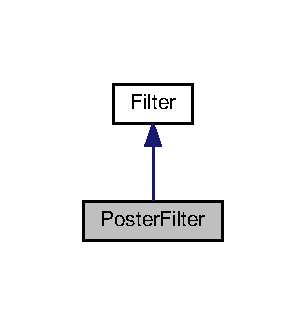
\includegraphics[width=147pt]{classModel_1_1PosterFilter__inherit__graph}
\end{center}
\end{figure}
\subsection*{Public Member Functions}
\begin{DoxyCompactItemize}
\item 
\hyperlink{classModel_1_1PosterFilter_a89cbfd099a8599b9b532d9c6a41fb997}{Poster\+Filter} ()
\item 
string \hyperlink{classModel_1_1PosterFilter_a62b7b60e24f92234393b840b35808e06}{get\+Filter\+Description} ()
\item 
int \hyperlink{classModel_1_1PosterFilter_ab9202ba7e871cc8488f73a14e4e6abef}{get\+Number\+Of\+Colors} ()
\item 
string \hyperlink{classModel_1_1PosterFilter_a11335e13e50af74108bf926dc1340b4b}{get\+Name} ()
\item 
void \hyperlink{classModel_1_1PosterFilter_a9a597e8af55b56d749dc67c3547a8d4e}{set\+Number\+Of\+Colors} (int \hyperlink{classModel_1_1PosterFilter_a84c387dad5d95eb7a12dbf283910935c}{number\+Of\+Colors})
\end{DoxyCompactItemize}
\subsection*{Private Attributes}
\begin{DoxyCompactItemize}
\item 
int \hyperlink{classModel_1_1PosterFilter_a84c387dad5d95eb7a12dbf283910935c}{number\+Of\+Colors}
\end{DoxyCompactItemize}
\subsection*{Additional Inherited Members}


\subsection{Detailed Description}
Reduces the maximum number of colors in the video. 

\subsection{Constructor \& Destructor Documentation}
\hypertarget{classModel_1_1PosterFilter_a89cbfd099a8599b9b532d9c6a41fb997}{}\index{Model\+::\+Poster\+Filter@{Model\+::\+Poster\+Filter}!Poster\+Filter@{Poster\+Filter}}
\index{Poster\+Filter@{Poster\+Filter}!Model\+::\+Poster\+Filter@{Model\+::\+Poster\+Filter}}
\subsubsection[{Poster\+Filter}]{\setlength{\rightskip}{0pt plus 5cm}{\bf Poster\+Filter} (
\begin{DoxyParamCaption}
{}
\end{DoxyParamCaption}
)}\label{classModel_1_1PosterFilter_a89cbfd099a8599b9b532d9c6a41fb997}


Constructor. 



\subsection{Member Function Documentation}
\hypertarget{classModel_1_1PosterFilter_a62b7b60e24f92234393b840b35808e06}{}\index{Model\+::\+Poster\+Filter@{Model\+::\+Poster\+Filter}!get\+Filter\+Description@{get\+Filter\+Description}}
\index{get\+Filter\+Description@{get\+Filter\+Description}!Model\+::\+Poster\+Filter@{Model\+::\+Poster\+Filter}}
\subsubsection[{get\+Filter\+Description}]{\setlength{\rightskip}{0pt plus 5cm}string get\+Filter\+Description (
\begin{DoxyParamCaption}
{}
\end{DoxyParamCaption}
)\hspace{0.3cm}{\ttfamily [virtual]}}\label{classModel_1_1PosterFilter_a62b7b60e24f92234393b840b35808e06}


Returns the string that the ffmpeg library needs to apply the filter to a video. 

\begin{DoxyReturn}{Returns}
The string for the ffmpeg library.
\end{DoxyReturn}


Implements \hyperlink{classModel_1_1Filter_a453fcafa809afa1ce58d9ef95d5f26c0}{Filter}.

\hypertarget{classModel_1_1PosterFilter_a11335e13e50af74108bf926dc1340b4b}{}\index{Model\+::\+Poster\+Filter@{Model\+::\+Poster\+Filter}!get\+Name@{get\+Name}}
\index{get\+Name@{get\+Name}!Model\+::\+Poster\+Filter@{Model\+::\+Poster\+Filter}}
\subsubsection[{get\+Name}]{\setlength{\rightskip}{0pt plus 5cm}string get\+Name (
\begin{DoxyParamCaption}
{}
\end{DoxyParamCaption}
)\hspace{0.3cm}{\ttfamily [virtual]}}\label{classModel_1_1PosterFilter_a11335e13e50af74108bf926dc1340b4b}


Returns the name of the filter. 

\begin{DoxyReturn}{Returns}
The filtername.
\end{DoxyReturn}


Implements \hyperlink{classModel_1_1Filter_ade93aa98c68d185a9c03784d36140225}{Filter}.

\hypertarget{classModel_1_1PosterFilter_ab9202ba7e871cc8488f73a14e4e6abef}{}\index{Model\+::\+Poster\+Filter@{Model\+::\+Poster\+Filter}!get\+Number\+Of\+Colors@{get\+Number\+Of\+Colors}}
\index{get\+Number\+Of\+Colors@{get\+Number\+Of\+Colors}!Model\+::\+Poster\+Filter@{Model\+::\+Poster\+Filter}}
\subsubsection[{get\+Number\+Of\+Colors}]{\setlength{\rightskip}{0pt plus 5cm}int get\+Number\+Of\+Colors (
\begin{DoxyParamCaption}
{}
\end{DoxyParamCaption}
)}\label{classModel_1_1PosterFilter_ab9202ba7e871cc8488f73a14e4e6abef}


Returns the maximum number of colors. 

\begin{DoxyReturn}{Returns}
Maximum number of colors.
\end{DoxyReturn}
\hypertarget{classModel_1_1PosterFilter_a9a597e8af55b56d749dc67c3547a8d4e}{}\index{Model\+::\+Poster\+Filter@{Model\+::\+Poster\+Filter}!set\+Number\+Of\+Colors@{set\+Number\+Of\+Colors}}
\index{set\+Number\+Of\+Colors@{set\+Number\+Of\+Colors}!Model\+::\+Poster\+Filter@{Model\+::\+Poster\+Filter}}
\subsubsection[{set\+Number\+Of\+Colors}]{\setlength{\rightskip}{0pt plus 5cm}void set\+Number\+Of\+Colors (
\begin{DoxyParamCaption}
\item[{int}]{number\+Of\+Colors}
\end{DoxyParamCaption}
)}\label{classModel_1_1PosterFilter_a9a597e8af55b56d749dc67c3547a8d4e}


Sets the maximum number of colors. 


\begin{DoxyParams}{Parameters}
{\em number\+Of\+Colors} & Maximum number of colors.\\
\hline
\end{DoxyParams}


\subsection{Field Documentation}
\hypertarget{classModel_1_1PosterFilter_a84c387dad5d95eb7a12dbf283910935c}{}\index{Model\+::\+Poster\+Filter@{Model\+::\+Poster\+Filter}!number\+Of\+Colors@{number\+Of\+Colors}}
\index{number\+Of\+Colors@{number\+Of\+Colors}!Model\+::\+Poster\+Filter@{Model\+::\+Poster\+Filter}}
\subsubsection[{number\+Of\+Colors}]{\setlength{\rightskip}{0pt plus 5cm}int number\+Of\+Colors\hspace{0.3cm}{\ttfamily [private]}}\label{classModel_1_1PosterFilter_a84c387dad5d95eb7a12dbf283910935c}

\newpage\hypertarget{classGUI_1_1PosterFilterBox}{}\section{Poster\+Filter\+Box Class Reference}
\label{classGUI_1_1PosterFilterBox}\index{Poster\+Filter\+Box@{Poster\+Filter\+Box}}
\subsection*{Public Member Functions}
\begin{DoxyCompactItemize}
\item 
\hypertarget{classGUI_1_1PosterFilterBox_adf0695b68fe68bc89275fea4168d796c}{}{\bfseries Poster\+Filter\+Box} (\hyperlink{classGUI_1_1QtGui_1_1QWidget____10}{G\+U\+I\+::\+Qt\+Gui\+::\+Q\+Widget\+\_\+\+\_\+10} $\ast$parent)\label{classGUI_1_1PosterFilterBox_adf0695b68fe68bc89275fea4168d796c}

\item 
\hypertarget{classGUI_1_1PosterFilterBox_ad7c0ee00fe3faac7942d75eec2a5342b}{}virtual void {\bfseries set\+Filter} (\hyperlink{classModel_1_1Filter_1_1Filter}{Model\+::\+Filter\+::\+Filter} \&filter)\label{classGUI_1_1PosterFilterBox_ad7c0ee00fe3faac7942d75eec2a5342b}

\item 
\hypertarget{classGUI_1_1PosterFilterBox_acef2029a93f4ab3a538cdb643b9c2613}{}virtual \hyperlink{classModel_1_1Filter_1_1Filter}{Model\+::\+Filter\+::\+Filter} $\ast$ {\bfseries get\+Filter} ()\label{classGUI_1_1PosterFilterBox_acef2029a93f4ab3a538cdb643b9c2613}

\end{DoxyCompactItemize}

\newpage\hypertarget{classGUI_1_1PreviewControlPanel}{}\section{Preview\+Control\+Panel Class Reference}
\label{classGUI_1_1PreviewControlPanel}\index{Preview\+Control\+Panel@{Preview\+Control\+Panel}}


Inheritance diagram for Preview\+Control\+Panel\+:
\nopagebreak
\begin{figure}[H]
\begin{center}
\leavevmode
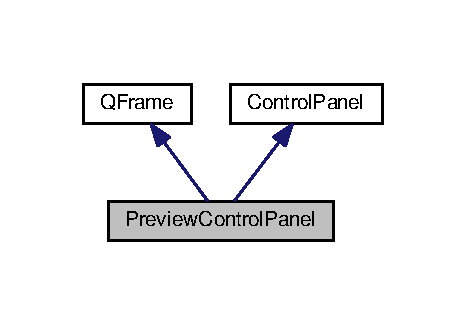
\includegraphics[width=224pt]{classGUI_1_1PreviewControlPanel__inherit__graph}
\end{center}
\end{figure}
\subsection*{Public Member Functions}
\begin{DoxyCompactItemize}
\item 
\hyperlink{classGUI_1_1PreviewControlPanel_adb0b94dcda87084c57e1f2b8fe268b73}{Preview\+Control\+Panel} (\hyperlink{classGUI_1_1QWidget}{G\+U\+I\+::\+Q\+Widget} $\ast$parent=0)
\item 
void \hyperlink{classGUI_1_1PreviewControlPanel_ae13c7f95f1ceda0fec18d18c3d7619f6}{update\+Ui} ()
\end{DoxyCompactItemize}
\subsection*{Private Member Functions}
\begin{DoxyCompactItemize}
\item 
void \hyperlink{classGUI_1_1PreviewControlPanel_aa72182c9a958af0e87b65ab7bdba0035}{create\+Ui} ()
\item 
void \hyperlink{classGUI_1_1PreviewControlPanel_a5176c9496a29e21eacb0f81ca1a29923}{create\+Actions} ()
\item 
void \hyperlink{classGUI_1_1PreviewControlPanel_a365329da56f8b07f8c95027ba967bbc3}{next\+Frame} ()
\item 
void \hyperlink{classGUI_1_1PreviewControlPanel_a3c96ed37c70ebc0b32c527a04e1536d1}{previous\+Frame} ()
\item 
void \hyperlink{classGUI_1_1PreviewControlPanel_a4b536406380edddc11ac215715dce3ea}{update\+Label} ()
\end{DoxyCompactItemize}
\subsection*{Private Attributes}
\begin{DoxyCompactItemize}
\item 
Q\+Push\+Button $\ast$ \hyperlink{classGUI_1_1PreviewControlPanel_a13676b392df866080d4a9a0b42f0c8a8}{button\+\_\+next\+Frame}
\item 
Q\+Push\+Button $\ast$ \hyperlink{classGUI_1_1PreviewControlPanel_a94ca89bf967e4f6fab20899a9e03347e}{button\+\_\+previous\+Frame}
\item 
Q\+Label $\ast$ \hyperlink{classGUI_1_1PreviewControlPanel_a9ee6b83724dafb50547cc6d3f90c2da3}{label\+\_\+position}
\end{DoxyCompactItemize}
\subsection*{Additional Inherited Members}


\subsection{Detailed Description}
This class is the control panel for the frame preview. 

\subsection{Constructor \& Destructor Documentation}
\hypertarget{classGUI_1_1PreviewControlPanel_adb0b94dcda87084c57e1f2b8fe268b73}{}\index{G\+U\+I\+::\+Preview\+Control\+Panel@{G\+U\+I\+::\+Preview\+Control\+Panel}!Preview\+Control\+Panel@{Preview\+Control\+Panel}}
\index{Preview\+Control\+Panel@{Preview\+Control\+Panel}!G\+U\+I\+::\+Preview\+Control\+Panel@{G\+U\+I\+::\+Preview\+Control\+Panel}}
\subsubsection[{Preview\+Control\+Panel}]{\setlength{\rightskip}{0pt plus 5cm}{\bf Preview\+Control\+Panel} (
\begin{DoxyParamCaption}
\item[{{\bf G\+U\+I\+::\+Q\+Widget} $\ast$}]{parent = {\ttfamily 0}}
\end{DoxyParamCaption}
)}\label{classGUI_1_1PreviewControlPanel_adb0b94dcda87084c57e1f2b8fe268b73}


Constructor. 



\subsection{Member Function Documentation}
\hypertarget{classGUI_1_1PreviewControlPanel_a5176c9496a29e21eacb0f81ca1a29923}{}\index{G\+U\+I\+::\+Preview\+Control\+Panel@{G\+U\+I\+::\+Preview\+Control\+Panel}!create\+Actions@{create\+Actions}}
\index{create\+Actions@{create\+Actions}!G\+U\+I\+::\+Preview\+Control\+Panel@{G\+U\+I\+::\+Preview\+Control\+Panel}}
\subsubsection[{create\+Actions}]{\setlength{\rightskip}{0pt plus 5cm}void create\+Actions (
\begin{DoxyParamCaption}
{}
\end{DoxyParamCaption}
)\hspace{0.3cm}{\ttfamily [private]}}\label{classGUI_1_1PreviewControlPanel_a5176c9496a29e21eacb0f81ca1a29923}


Creates the actions. 

\hypertarget{classGUI_1_1PreviewControlPanel_aa72182c9a958af0e87b65ab7bdba0035}{}\index{G\+U\+I\+::\+Preview\+Control\+Panel@{G\+U\+I\+::\+Preview\+Control\+Panel}!create\+Ui@{create\+Ui}}
\index{create\+Ui@{create\+Ui}!G\+U\+I\+::\+Preview\+Control\+Panel@{G\+U\+I\+::\+Preview\+Control\+Panel}}
\subsubsection[{create\+Ui}]{\setlength{\rightskip}{0pt plus 5cm}void create\+Ui (
\begin{DoxyParamCaption}
{}
\end{DoxyParamCaption}
)\hspace{0.3cm}{\ttfamily [private]}}\label{classGUI_1_1PreviewControlPanel_aa72182c9a958af0e87b65ab7bdba0035}


Creates the ui. 

\hypertarget{classGUI_1_1PreviewControlPanel_a365329da56f8b07f8c95027ba967bbc3}{}\index{G\+U\+I\+::\+Preview\+Control\+Panel@{G\+U\+I\+::\+Preview\+Control\+Panel}!next\+Frame@{next\+Frame}}
\index{next\+Frame@{next\+Frame}!G\+U\+I\+::\+Preview\+Control\+Panel@{G\+U\+I\+::\+Preview\+Control\+Panel}}
\subsubsection[{next\+Frame}]{\setlength{\rightskip}{0pt plus 5cm}void next\+Frame (
\begin{DoxyParamCaption}
{}
\end{DoxyParamCaption}
)\hspace{0.3cm}{\ttfamily [private]}}\label{classGUI_1_1PreviewControlPanel_a365329da56f8b07f8c95027ba967bbc3}


Slot for button\+\_\+next\+Frame.\+clicked() signal. 

\hypertarget{classGUI_1_1PreviewControlPanel_a3c96ed37c70ebc0b32c527a04e1536d1}{}\index{G\+U\+I\+::\+Preview\+Control\+Panel@{G\+U\+I\+::\+Preview\+Control\+Panel}!previous\+Frame@{previous\+Frame}}
\index{previous\+Frame@{previous\+Frame}!G\+U\+I\+::\+Preview\+Control\+Panel@{G\+U\+I\+::\+Preview\+Control\+Panel}}
\subsubsection[{previous\+Frame}]{\setlength{\rightskip}{0pt plus 5cm}void previous\+Frame (
\begin{DoxyParamCaption}
{}
\end{DoxyParamCaption}
)\hspace{0.3cm}{\ttfamily [private]}}\label{classGUI_1_1PreviewControlPanel_a3c96ed37c70ebc0b32c527a04e1536d1}


Slot for button\+\_\+previous\+Frame.\+clicked() signal. 

\hypertarget{classGUI_1_1PreviewControlPanel_a4b536406380edddc11ac215715dce3ea}{}\index{G\+U\+I\+::\+Preview\+Control\+Panel@{G\+U\+I\+::\+Preview\+Control\+Panel}!update\+Label@{update\+Label}}
\index{update\+Label@{update\+Label}!G\+U\+I\+::\+Preview\+Control\+Panel@{G\+U\+I\+::\+Preview\+Control\+Panel}}
\subsubsection[{update\+Label}]{\setlength{\rightskip}{0pt plus 5cm}void update\+Label (
\begin{DoxyParamCaption}
{}
\end{DoxyParamCaption}
)\hspace{0.3cm}{\ttfamily [private]}}\label{classGUI_1_1PreviewControlPanel_a4b536406380edddc11ac215715dce3ea}


Updates the label that shows the current position. 

\hypertarget{classGUI_1_1PreviewControlPanel_ae13c7f95f1ceda0fec18d18c3d7619f6}{}\index{G\+U\+I\+::\+Preview\+Control\+Panel@{G\+U\+I\+::\+Preview\+Control\+Panel}!update\+Ui@{update\+Ui}}
\index{update\+Ui@{update\+Ui}!G\+U\+I\+::\+Preview\+Control\+Panel@{G\+U\+I\+::\+Preview\+Control\+Panel}}
\subsubsection[{update\+Ui}]{\setlength{\rightskip}{0pt plus 5cm}void update\+Ui (
\begin{DoxyParamCaption}
{}
\end{DoxyParamCaption}
)\hspace{0.3cm}{\ttfamily [virtual]}}\label{classGUI_1_1PreviewControlPanel_ae13c7f95f1ceda0fec18d18c3d7619f6}


Updates the ui of the control panel. 



Implements \hyperlink{classGUI_1_1ControlPanel_aa9963358cf9cff5ea2531d73efa78f73}{Control\+Panel}.



\subsection{Field Documentation}
\hypertarget{classGUI_1_1PreviewControlPanel_a13676b392df866080d4a9a0b42f0c8a8}{}\index{G\+U\+I\+::\+Preview\+Control\+Panel@{G\+U\+I\+::\+Preview\+Control\+Panel}!button\+\_\+next\+Frame@{button\+\_\+next\+Frame}}
\index{button\+\_\+next\+Frame@{button\+\_\+next\+Frame}!G\+U\+I\+::\+Preview\+Control\+Panel@{G\+U\+I\+::\+Preview\+Control\+Panel}}
\subsubsection[{button\+\_\+next\+Frame}]{\setlength{\rightskip}{0pt plus 5cm}Q\+Push\+Button$\ast$ button\+\_\+next\+Frame\hspace{0.3cm}{\ttfamily [private]}}\label{classGUI_1_1PreviewControlPanel_a13676b392df866080d4a9a0b42f0c8a8}
\hypertarget{classGUI_1_1PreviewControlPanel_a94ca89bf967e4f6fab20899a9e03347e}{}\index{G\+U\+I\+::\+Preview\+Control\+Panel@{G\+U\+I\+::\+Preview\+Control\+Panel}!button\+\_\+previous\+Frame@{button\+\_\+previous\+Frame}}
\index{button\+\_\+previous\+Frame@{button\+\_\+previous\+Frame}!G\+U\+I\+::\+Preview\+Control\+Panel@{G\+U\+I\+::\+Preview\+Control\+Panel}}
\subsubsection[{button\+\_\+previous\+Frame}]{\setlength{\rightskip}{0pt plus 5cm}Q\+Push\+Button$\ast$ button\+\_\+previous\+Frame\hspace{0.3cm}{\ttfamily [private]}}\label{classGUI_1_1PreviewControlPanel_a94ca89bf967e4f6fab20899a9e03347e}
\hypertarget{classGUI_1_1PreviewControlPanel_a9ee6b83724dafb50547cc6d3f90c2da3}{}\index{G\+U\+I\+::\+Preview\+Control\+Panel@{G\+U\+I\+::\+Preview\+Control\+Panel}!label\+\_\+position@{label\+\_\+position}}
\index{label\+\_\+position@{label\+\_\+position}!G\+U\+I\+::\+Preview\+Control\+Panel@{G\+U\+I\+::\+Preview\+Control\+Panel}}
\subsubsection[{label\+\_\+position}]{\setlength{\rightskip}{0pt plus 5cm}Q\+Label$\ast$ label\+\_\+position\hspace{0.3cm}{\ttfamily [private]}}\label{classGUI_1_1PreviewControlPanel_a9ee6b83724dafb50547cc6d3f90c2da3}

\newpage\hypertarget{classModel_1_1Project}{}\section{Project Class Reference}
\label{classModel_1_1Project}\index{Project@{Project}}
\subsection*{Public Member Functions}
\begin{DoxyCompactItemize}
\item 
\hyperlink{classModel_1_1Project_ae247a6a7beaace2e9d2637521160002c}{Project} (Q\+String name)
\item 
Q\+String \hyperlink{classModel_1_1Project_ab6b223a95a460d422d940396d9a5657b}{get\+Name} ()
\item 
\hyperlink{classMemento_1_1MainWindowMemento}{Memento\+::\+Main\+Window\+Memento} \& \hyperlink{classModel_1_1Project_a439f54da110f371207bbedac6fe64bf0}{get\+Memento} ()
\item 
void \hyperlink{classModel_1_1Project_a06dcc543cbe7f60ea6a1da13d2585964}{set\+Memento} (\hyperlink{classMemento_1_1MainWindowMemento}{Memento\+::\+Main\+Window\+Memento} memento)
\item 
void \hyperlink{classModel_1_1Project_a41d3b419f9a56edd2854fb27715c94d5}{set\+Path} (Q\+String path)
\item 
Q\+String \hyperlink{classModel_1_1Project_a1a94d0c9bf9dd725556721ac914025e3}{get\+Path} ()
\end{DoxyCompactItemize}


\subsection{Detailed Description}
This class contains the different mementos. 

\subsection{Constructor \& Destructor Documentation}
\hypertarget{classModel_1_1Project_ae247a6a7beaace2e9d2637521160002c}{}\index{Model\+::\+Project@{Model\+::\+Project}!Project@{Project}}
\index{Project@{Project}!Model\+::\+Project@{Model\+::\+Project}}
\subsubsection[{Project}]{\setlength{\rightskip}{0pt plus 5cm}{\bf Project} (
\begin{DoxyParamCaption}
\item[{Q\+String}]{name}
\end{DoxyParamCaption}
)}\label{classModel_1_1Project_ae247a6a7beaace2e9d2637521160002c}


Constructor. 


\begin{DoxyParams}{Parameters}
{\em name} & Name of the project.\\
\hline
\end{DoxyParams}


\subsection{Member Function Documentation}
\hypertarget{classModel_1_1Project_a439f54da110f371207bbedac6fe64bf0}{}\index{Model\+::\+Project@{Model\+::\+Project}!get\+Memento@{get\+Memento}}
\index{get\+Memento@{get\+Memento}!Model\+::\+Project@{Model\+::\+Project}}
\subsubsection[{get\+Memento}]{\setlength{\rightskip}{0pt plus 5cm}{\bf Memento\+::\+Main\+Window\+Memento} \& get\+Memento (
\begin{DoxyParamCaption}
{}
\end{DoxyParamCaption}
)}\label{classModel_1_1Project_a439f54da110f371207bbedac6fe64bf0}


Returns the Main\+Window\+Memento. 

\begin{DoxyReturn}{Returns}
The Main\+Window\+Memento.
\end{DoxyReturn}
\hypertarget{classModel_1_1Project_ab6b223a95a460d422d940396d9a5657b}{}\index{Model\+::\+Project@{Model\+::\+Project}!get\+Name@{get\+Name}}
\index{get\+Name@{get\+Name}!Model\+::\+Project@{Model\+::\+Project}}
\subsubsection[{get\+Name}]{\setlength{\rightskip}{0pt plus 5cm}Q\+String get\+Name (
\begin{DoxyParamCaption}
{}
\end{DoxyParamCaption}
)}\label{classModel_1_1Project_ab6b223a95a460d422d940396d9a5657b}


Returns the name of the project. 

\begin{DoxyReturn}{Returns}
Name of the project.
\end{DoxyReturn}
\hypertarget{classModel_1_1Project_a1a94d0c9bf9dd725556721ac914025e3}{}\index{Model\+::\+Project@{Model\+::\+Project}!get\+Path@{get\+Path}}
\index{get\+Path@{get\+Path}!Model\+::\+Project@{Model\+::\+Project}}
\subsubsection[{get\+Path}]{\setlength{\rightskip}{0pt plus 5cm}Q\+String get\+Path (
\begin{DoxyParamCaption}
{}
\end{DoxyParamCaption}
)}\label{classModel_1_1Project_a1a94d0c9bf9dd725556721ac914025e3}


Returns the project save path. 

\begin{DoxyReturn}{Returns}
The project save path.
\end{DoxyReturn}
\hypertarget{classModel_1_1Project_a06dcc543cbe7f60ea6a1da13d2585964}{}\index{Model\+::\+Project@{Model\+::\+Project}!set\+Memento@{set\+Memento}}
\index{set\+Memento@{set\+Memento}!Model\+::\+Project@{Model\+::\+Project}}
\subsubsection[{set\+Memento}]{\setlength{\rightskip}{0pt plus 5cm}void set\+Memento (
\begin{DoxyParamCaption}
\item[{{\bf Memento\+::\+Main\+Window\+Memento}}]{memento}
\end{DoxyParamCaption}
)}\label{classModel_1_1Project_a06dcc543cbe7f60ea6a1da13d2585964}


Sets the Main\+Window\+Memento. 


\begin{DoxyParams}{Parameters}
{\em memento} & The Main\+Window\+Memento.\\
\hline
\end{DoxyParams}
\hypertarget{classModel_1_1Project_a41d3b419f9a56edd2854fb27715c94d5}{}\index{Model\+::\+Project@{Model\+::\+Project}!set\+Path@{set\+Path}}
\index{set\+Path@{set\+Path}!Model\+::\+Project@{Model\+::\+Project}}
\subsubsection[{set\+Path}]{\setlength{\rightskip}{0pt plus 5cm}void set\+Path (
\begin{DoxyParamCaption}
\item[{Q\+String}]{path}
\end{DoxyParamCaption}
)}\label{classModel_1_1Project_a41d3b419f9a56edd2854fb27715c94d5}


Sets the path at which the project is saved. 


\begin{DoxyParams}{Parameters}
{\em path} & The project save path.\\
\hline
\end{DoxyParams}

\newpage\hypertarget{classUtility_1_1ProjectReader}{}\section{Project\+Reader Class Reference}
\label{classUtility_1_1ProjectReader}\index{Project\+Reader@{Project\+Reader}}
\subsection*{Public Member Functions}
\begin{DoxyCompactItemize}
\item 
\hyperlink{classUtility_1_1ProjectReader_a94102c58bc458c982fd7a306aff6b219}{Project\+Reader} (Q\+String path)
\item 
\hyperlink{classModel_1_1Project}{Model\+::\+Project} \hyperlink{classUtility_1_1ProjectReader_a953be173fb9970cd135db295767a4dcd}{read\+Project} ()
\end{DoxyCompactItemize}


\subsection{Detailed Description}
This class can read a project from a file. 

\subsection{Constructor \& Destructor Documentation}
\hypertarget{classUtility_1_1ProjectReader_a94102c58bc458c982fd7a306aff6b219}{}\index{Utility\+::\+Project\+Reader@{Utility\+::\+Project\+Reader}!Project\+Reader@{Project\+Reader}}
\index{Project\+Reader@{Project\+Reader}!Utility\+::\+Project\+Reader@{Utility\+::\+Project\+Reader}}
\subsubsection[{Project\+Reader}]{\setlength{\rightskip}{0pt plus 5cm}{\bf Project\+Reader} (
\begin{DoxyParamCaption}
\item[{Q\+String}]{path}
\end{DoxyParamCaption}
)}\label{classUtility_1_1ProjectReader_a94102c58bc458c982fd7a306aff6b219}


Constructor. 


\begin{DoxyParams}{Parameters}
{\em path} & The absolute path to the project file.\\
\hline
\end{DoxyParams}


\subsection{Member Function Documentation}
\hypertarget{classUtility_1_1ProjectReader_a953be173fb9970cd135db295767a4dcd}{}\index{Utility\+::\+Project\+Reader@{Utility\+::\+Project\+Reader}!read\+Project@{read\+Project}}
\index{read\+Project@{read\+Project}!Utility\+::\+Project\+Reader@{Utility\+::\+Project\+Reader}}
\subsubsection[{read\+Project}]{\setlength{\rightskip}{0pt plus 5cm}{\bf Model\+::\+Project} read\+Project (
\begin{DoxyParamCaption}
{}
\end{DoxyParamCaption}
)}\label{classUtility_1_1ProjectReader_a953be173fb9970cd135db295767a4dcd}


Reads a project from a file. 

\begin{DoxyReturn}{Returns}
The loaded project.
\end{DoxyReturn}

\newpage\hypertarget{classUtility_1_1ProjectWriter}{}\section{Project\+Writer Class Reference}
\label{classUtility_1_1ProjectWriter}\index{Project\+Writer@{Project\+Writer}}
\subsection*{Public Member Functions}
\begin{DoxyCompactItemize}
\item 
\hyperlink{classUtility_1_1ProjectWriter_a28aa961d1450c80077122b50691204ad}{Project\+Writer} (\hyperlink{classModel_1_1Project}{Model\+::\+Project} p)
\item 
void \hyperlink{classUtility_1_1ProjectWriter_a5de2650de39370a5fe89f8d918966276}{save\+Project} ()
\item 
void \hyperlink{classUtility_1_1ProjectWriter_a5c087450ee93776fd121b0fd6af473e6}{save\+Results} ()
\end{DoxyCompactItemize}


\subsection{Detailed Description}
This class can write the project files and the results. 

\subsection{Constructor \& Destructor Documentation}
\hypertarget{classUtility_1_1ProjectWriter_a28aa961d1450c80077122b50691204ad}{}\index{Utility\+::\+Project\+Writer@{Utility\+::\+Project\+Writer}!Project\+Writer@{Project\+Writer}}
\index{Project\+Writer@{Project\+Writer}!Utility\+::\+Project\+Writer@{Utility\+::\+Project\+Writer}}
\subsubsection[{Project\+Writer}]{\setlength{\rightskip}{0pt plus 5cm}{\bf Project\+Writer} (
\begin{DoxyParamCaption}
\item[{{\bf Model\+::\+Project}}]{p}
\end{DoxyParamCaption}
)}\label{classUtility_1_1ProjectWriter_a28aa961d1450c80077122b50691204ad}


Constructor. 


\begin{DoxyParams}{Parameters}
{\em p} & The project to save.\\
\hline
\end{DoxyParams}


\subsection{Member Function Documentation}
\hypertarget{classUtility_1_1ProjectWriter_a5de2650de39370a5fe89f8d918966276}{}\index{Utility\+::\+Project\+Writer@{Utility\+::\+Project\+Writer}!save\+Project@{save\+Project}}
\index{save\+Project@{save\+Project}!Utility\+::\+Project\+Writer@{Utility\+::\+Project\+Writer}}
\subsubsection[{save\+Project}]{\setlength{\rightskip}{0pt plus 5cm}void save\+Project (
\begin{DoxyParamCaption}
{}
\end{DoxyParamCaption}
)}\label{classUtility_1_1ProjectWriter_a5de2650de39370a5fe89f8d918966276}


Saves the whole project. 

\hypertarget{classUtility_1_1ProjectWriter_a5c087450ee93776fd121b0fd6af473e6}{}\index{Utility\+::\+Project\+Writer@{Utility\+::\+Project\+Writer}!save\+Results@{save\+Results}}
\index{save\+Results@{save\+Results}!Utility\+::\+Project\+Writer@{Utility\+::\+Project\+Writer}}
\subsubsection[{save\+Results}]{\setlength{\rightskip}{0pt plus 5cm}void save\+Results (
\begin{DoxyParamCaption}
{}
\end{DoxyParamCaption}
)}\label{classUtility_1_1ProjectWriter_a5c087450ee93776fd121b0fd6af473e6}


Saves on the analysis results. 


\newpage\hypertarget{classUtility_1_1PsnrCalculator}{}\section{Psnr\+Calculator Class Reference}
\label{classUtility_1_1PsnrCalculator}\index{Psnr\+Calculator@{Psnr\+Calculator}}
\subsection*{Public Member Functions}
\begin{DoxyCompactItemize}
\item 
\hyperlink{classUtility_1_1PsnrCalculator_af9b7f590502107d7fa40cfb6288287f5}{Psnr\+Calculator} (\hyperlink{classModel_1_1AVVideo}{Model\+::\+A\+V\+Video} \&\hyperlink{classUtility_1_1PsnrCalculator_ac18ce56ef484f4499434c4b5c5fafc8a}{reference\+Video}, \hyperlink{classModel_1_1AVVideo}{Model\+::\+A\+V\+Video} \&compare\+Video)
\item 
\hyperlink{classModel_1_1Graph}{Model\+::\+Graph} \hyperlink{classUtility_1_1PsnrCalculator_add29b5117d03aca3e7bb3199edc95cd5}{calculate} ()
\end{DoxyCompactItemize}
\subsection*{Private Member Functions}
\begin{DoxyCompactItemize}
\item 
void \hyperlink{classUtility_1_1PsnrCalculator_a02fd73d861ef2e4aabb38c0c9ff82947}{init} ()
\end{DoxyCompactItemize}
\subsection*{Private Attributes}
\begin{DoxyCompactItemize}
\item 
\hyperlink{classModel_1_1AVVideo}{Model\+::\+A\+V\+Video} $\ast$ \hyperlink{classUtility_1_1PsnrCalculator_ac18ce56ef484f4499434c4b5c5fafc8a}{reference\+Video}
\item 
\hyperlink{classModel_1_1AVVideo}{Model\+::\+A\+V\+Video} $\ast$ \hyperlink{classUtility_1_1PsnrCalculator_a9d9339a030e5aa3b959eecf241b6ffac}{video}
\end{DoxyCompactItemize}


\subsection{Detailed Description}
This class calculates the psnr-\/graph of a video. 

\subsection{Constructor \& Destructor Documentation}
\hypertarget{classUtility_1_1PsnrCalculator_af9b7f590502107d7fa40cfb6288287f5}{}\index{Utility\+::\+Psnr\+Calculator@{Utility\+::\+Psnr\+Calculator}!Psnr\+Calculator@{Psnr\+Calculator}}
\index{Psnr\+Calculator@{Psnr\+Calculator}!Utility\+::\+Psnr\+Calculator@{Utility\+::\+Psnr\+Calculator}}
\subsubsection[{Psnr\+Calculator}]{\setlength{\rightskip}{0pt plus 5cm}{\bf Psnr\+Calculator} (
\begin{DoxyParamCaption}
\item[{{\bf Model\+::\+A\+V\+Video} \&}]{reference\+Video, }
\item[{{\bf Model\+::\+A\+V\+Video} \&}]{compare\+Video}
\end{DoxyParamCaption}
)}\label{classUtility_1_1PsnrCalculator_af9b7f590502107d7fa40cfb6288287f5}


Constructor. 


\begin{DoxyParams}{Parameters}
{\em reference\+Video} & The reference video for the psnr calculation.\\
\hline
{\em compare\+Video} & The video that is compared to the reference video.\\
\hline
\end{DoxyParams}


\subsection{Member Function Documentation}
\hypertarget{classUtility_1_1PsnrCalculator_add29b5117d03aca3e7bb3199edc95cd5}{}\index{Utility\+::\+Psnr\+Calculator@{Utility\+::\+Psnr\+Calculator}!calculate@{calculate}}
\index{calculate@{calculate}!Utility\+::\+Psnr\+Calculator@{Utility\+::\+Psnr\+Calculator}}
\subsubsection[{calculate}]{\setlength{\rightskip}{0pt plus 5cm}{\bf Model\+::\+Graph} calculate (
\begin{DoxyParamCaption}
{}
\end{DoxyParamCaption}
)}\label{classUtility_1_1PsnrCalculator_add29b5117d03aca3e7bb3199edc95cd5}


Calculates the psnr graph. 

\begin{DoxyReturn}{Returns}
The calculated psnr graph.
\end{DoxyReturn}
\hypertarget{classUtility_1_1PsnrCalculator_a02fd73d861ef2e4aabb38c0c9ff82947}{}\index{Utility\+::\+Psnr\+Calculator@{Utility\+::\+Psnr\+Calculator}!init@{init}}
\index{init@{init}!Utility\+::\+Psnr\+Calculator@{Utility\+::\+Psnr\+Calculator}}
\subsubsection[{init}]{\setlength{\rightskip}{0pt plus 5cm}void init (
\begin{DoxyParamCaption}
{}
\end{DoxyParamCaption}
)\hspace{0.3cm}{\ttfamily [private]}}\label{classUtility_1_1PsnrCalculator_a02fd73d861ef2e4aabb38c0c9ff82947}


Initializes the ffmpeg psnr filter. 



\subsection{Field Documentation}
\hypertarget{classUtility_1_1PsnrCalculator_ac18ce56ef484f4499434c4b5c5fafc8a}{}\index{Utility\+::\+Psnr\+Calculator@{Utility\+::\+Psnr\+Calculator}!reference\+Video@{reference\+Video}}
\index{reference\+Video@{reference\+Video}!Utility\+::\+Psnr\+Calculator@{Utility\+::\+Psnr\+Calculator}}
\subsubsection[{reference\+Video}]{\setlength{\rightskip}{0pt plus 5cm}{\bf Model\+::\+A\+V\+Video}$\ast$ reference\+Video\hspace{0.3cm}{\ttfamily [private]}}\label{classUtility_1_1PsnrCalculator_ac18ce56ef484f4499434c4b5c5fafc8a}
\hypertarget{classUtility_1_1PsnrCalculator_a9d9339a030e5aa3b959eecf241b6ffac}{}\index{Utility\+::\+Psnr\+Calculator@{Utility\+::\+Psnr\+Calculator}!video@{video}}
\index{video@{video}!Utility\+::\+Psnr\+Calculator@{Utility\+::\+Psnr\+Calculator}}
\subsubsection[{video}]{\setlength{\rightskip}{0pt plus 5cm}{\bf Model\+::\+A\+V\+Video}$\ast$ video\hspace{0.3cm}{\ttfamily [private]}}\label{classUtility_1_1PsnrCalculator_a9d9339a030e5aa3b959eecf241b6ffac}

\newpage\hypertarget{classGUI_1_1QCheckBox}{}\section{Q\+Check\+Box Class Reference}
\label{classGUI_1_1QCheckBox}\index{Q\+Check\+Box@{Q\+Check\+Box}}

\newpage\hypertarget{classGUI_1_1QComboBox}{}\section{Q\+Combo\+Box Class Reference}
\label{classGUI_1_1QComboBox}\index{Q\+Combo\+Box@{Q\+Combo\+Box}}

\newpage\hypertarget{classGUI_1_1QDialog}{}\section{Q\+Dialog Class Reference}
\label{classGUI_1_1QDialog}\index{Q\+Dialog@{Q\+Dialog}}


Inheritance diagram for Q\+Dialog\+:
\nopagebreak
\begin{figure}[H]
\begin{center}
\leavevmode
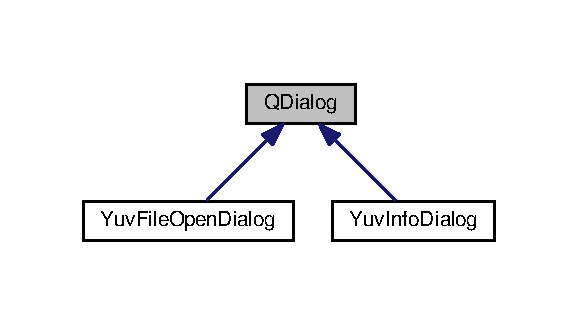
\includegraphics[width=278pt]{classGUI_1_1QDialog__inherit__graph}
\end{center}
\end{figure}

\newpage\hypertarget{classGUI_1_1QFrame}{}\section{Q\+Frame Class Reference}
\label{classGUI_1_1QFrame}\index{Q\+Frame@{Q\+Frame}}


Inheritance diagram for Q\+Frame\+:
\nopagebreak
\begin{figure}[H]
\begin{center}
\leavevmode
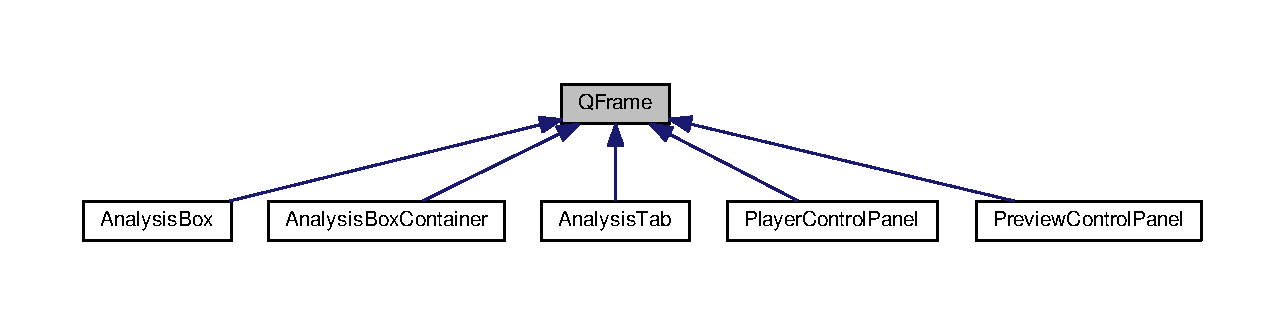
\includegraphics[width=350pt]{classGUI_1_1QFrame__inherit__graph}
\end{center}
\end{figure}

\newpage\hypertarget{classGUI_1_1QGraphicsView}{}\section{Q\+Graphics\+View Class Reference}
\label{classGUI_1_1QGraphicsView}\index{Q\+Graphics\+View@{Q\+Graphics\+View}}


Inheritance diagram for Q\+Graphics\+View\+:
\nopagebreak
\begin{figure}[H]
\begin{center}
\leavevmode
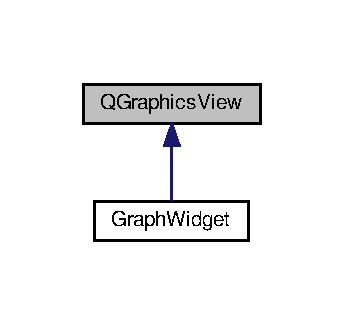
\includegraphics[width=165pt]{classGUI_1_1QGraphicsView__inherit__graph}
\end{center}
\end{figure}

\newpage\hypertarget{classGUI_1_1QMainWindow}{}\section{Q\+Main\+Window Class Reference}
\label{classGUI_1_1QMainWindow}\index{Q\+Main\+Window@{Q\+Main\+Window}}


Inheritance diagram for Q\+Main\+Window\+:
\nopagebreak
\begin{figure}[H]
\begin{center}
\leavevmode
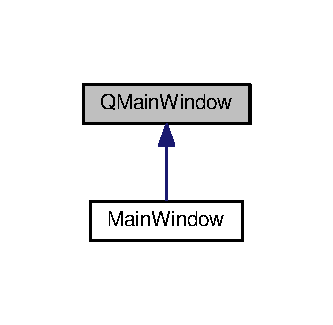
\includegraphics[width=160pt]{classGUI_1_1QMainWindow__inherit__graph}
\end{center}
\end{figure}

\newpage\hypertarget{classUndoRedo_1_1QUndoCommand}{}\section{Q\+Undo\+Command Class Reference}
\label{classUndoRedo_1_1QUndoCommand}\index{Q\+Undo\+Command@{Q\+Undo\+Command}}

\newpage\hypertarget{classGUI_1_1QWidget}{}\section{Q\+Widget Class Reference}
\label{classGUI_1_1QWidget}\index{Q\+Widget@{Q\+Widget}}


Inheritance diagram for Q\+Widget\+:
\nopagebreak
\begin{figure}[H]
\begin{center}
\leavevmode
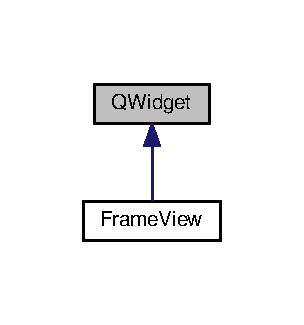
\includegraphics[width=146pt]{classGUI_1_1QWidget__inherit__graph}
\end{center}
\end{figure}

\newpage\hypertarget{classModel_1_1RectangleFilter}{}\section{Rectangle\+Filter Class Reference}
\label{classModel_1_1RectangleFilter}\index{Rectangle\+Filter@{Rectangle\+Filter}}


Inheritance diagram for Rectangle\+Filter\+:
\nopagebreak
\begin{figure}[H]
\begin{center}
\leavevmode
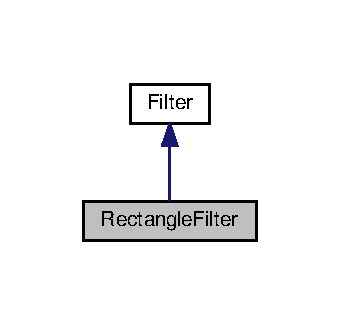
\includegraphics[width=163pt]{classModel_1_1RectangleFilter__inherit__graph}
\end{center}
\end{figure}
\subsection*{Public Member Functions}
\begin{DoxyCompactItemize}
\item 
\hyperlink{classModel_1_1RectangleFilter_a74b7006780424b64c299443d1b54fc03}{Rectangle\+Filter} ()
\item 
string \hyperlink{classModel_1_1RectangleFilter_a62b7b60e24f92234393b840b35808e06}{get\+Filter\+Description} ()
\item 
Q\+Rgb \hyperlink{classModel_1_1RectangleFilter_ae697defefbdf5f895406269b15758d91}{get\+Color} ()
\item 
void \hyperlink{classModel_1_1RectangleFilter_ad858846447f303e473dc8004ef607666}{set\+Color} (Q\+Rgb \hyperlink{classModel_1_1RectangleFilter_a6e0c08bd2043c82b2e837117d811db91}{color})
\item 
int \hyperlink{classModel_1_1RectangleFilter_a67a0997183f24da19b776d96c1052998}{get\+Width} ()
\item 
void \hyperlink{classModel_1_1RectangleFilter_a8b4c8bccc530aa0a9b0139e04913af32}{set\+Width} (int \hyperlink{classModel_1_1RectangleFilter_a2474a5474cbff19523a51eb1de01cda4}{width})
\item 
int \hyperlink{classModel_1_1RectangleFilter_a07efb2a4e9a982688c8bb3c3f21d1092}{get\+Height} ()
\item 
void \hyperlink{classModel_1_1RectangleFilter_a7013185ad2825ade83994b396c4fdfcd}{set\+Height} (int \hyperlink{classModel_1_1RectangleFilter_ad12fc34ce789bce6c8a05d8a17138534}{height})
\item 
int \hyperlink{classModel_1_1RectangleFilter_ae13f88e922e1339355456062ad9fa359}{get\+X} ()
\item 
string \hyperlink{classModel_1_1RectangleFilter_a11335e13e50af74108bf926dc1340b4b}{get\+Name} ()
\item 
void \hyperlink{classModel_1_1RectangleFilter_add2578ea6b65ad27a905a6d2048748bb}{set\+X} (int \hyperlink{classModel_1_1RectangleFilter_a6150e0515f7202e2fb518f7206ed97dc}{x})
\item 
int \hyperlink{classModel_1_1RectangleFilter_aab81944f0a14bba932c0931899951937}{get\+Y} ()
\item 
void \hyperlink{classModel_1_1RectangleFilter_adea78a9ff1234e75627dda61d972213b}{set\+Y} (int \hyperlink{classModel_1_1RectangleFilter_a0a2f84ed7838f07779ae24c5a9086d33}{y})
\item 
int \hyperlink{classModel_1_1RectangleFilter_a0c8618c617e65d5ab8400704bbc09ed1}{get\+Opacity} ()
\item 
void \hyperlink{classModel_1_1RectangleFilter_a22b140225648b55b27f2330938ae4006}{set\+Opacity} (int \hyperlink{classModel_1_1RectangleFilter_ab86f8ec3f0949a133a694bba7f166a05}{opacity})
\end{DoxyCompactItemize}
\subsection*{Private Attributes}
\begin{DoxyCompactItemize}
\item 
Q\+Rgb \hyperlink{classModel_1_1RectangleFilter_a6e0c08bd2043c82b2e837117d811db91}{color}
\item 
int \hyperlink{classModel_1_1RectangleFilter_a2474a5474cbff19523a51eb1de01cda4}{width}
\item 
int \hyperlink{classModel_1_1RectangleFilter_ad12fc34ce789bce6c8a05d8a17138534}{height}
\item 
int \hyperlink{classModel_1_1RectangleFilter_a6150e0515f7202e2fb518f7206ed97dc}{x}
\item 
int \hyperlink{classModel_1_1RectangleFilter_a0a2f84ed7838f07779ae24c5a9086d33}{y}
\item 
int \hyperlink{classModel_1_1RectangleFilter_ab86f8ec3f0949a133a694bba7f166a05}{opacity}
\end{DoxyCompactItemize}
\subsection*{Additional Inherited Members}


\subsection{Detailed Description}
Inserts a filled rectangle with a given color into the video 

\subsection{Constructor \& Destructor Documentation}
\hypertarget{classModel_1_1RectangleFilter_a74b7006780424b64c299443d1b54fc03}{}\index{Model\+::\+Rectangle\+Filter@{Model\+::\+Rectangle\+Filter}!Rectangle\+Filter@{Rectangle\+Filter}}
\index{Rectangle\+Filter@{Rectangle\+Filter}!Model\+::\+Rectangle\+Filter@{Model\+::\+Rectangle\+Filter}}
\subsubsection[{Rectangle\+Filter}]{\setlength{\rightskip}{0pt plus 5cm}{\bf Rectangle\+Filter} (
\begin{DoxyParamCaption}
{}
\end{DoxyParamCaption}
)}\label{classModel_1_1RectangleFilter_a74b7006780424b64c299443d1b54fc03}


Constructor. 



\subsection{Member Function Documentation}
\hypertarget{classModel_1_1RectangleFilter_ae697defefbdf5f895406269b15758d91}{}\index{Model\+::\+Rectangle\+Filter@{Model\+::\+Rectangle\+Filter}!get\+Color@{get\+Color}}
\index{get\+Color@{get\+Color}!Model\+::\+Rectangle\+Filter@{Model\+::\+Rectangle\+Filter}}
\subsubsection[{get\+Color}]{\setlength{\rightskip}{0pt plus 5cm}Q\+Rgb get\+Color (
\begin{DoxyParamCaption}
{}
\end{DoxyParamCaption}
)}\label{classModel_1_1RectangleFilter_ae697defefbdf5f895406269b15758d91}


Returns the color of the rectangle. 

\begin{DoxyReturn}{Returns}
The color of the rectangle.
\end{DoxyReturn}
\hypertarget{classModel_1_1RectangleFilter_a62b7b60e24f92234393b840b35808e06}{}\index{Model\+::\+Rectangle\+Filter@{Model\+::\+Rectangle\+Filter}!get\+Filter\+Description@{get\+Filter\+Description}}
\index{get\+Filter\+Description@{get\+Filter\+Description}!Model\+::\+Rectangle\+Filter@{Model\+::\+Rectangle\+Filter}}
\subsubsection[{get\+Filter\+Description}]{\setlength{\rightskip}{0pt plus 5cm}string get\+Filter\+Description (
\begin{DoxyParamCaption}
{}
\end{DoxyParamCaption}
)\hspace{0.3cm}{\ttfamily [virtual]}}\label{classModel_1_1RectangleFilter_a62b7b60e24f92234393b840b35808e06}


Returns the string that the ffmpeg library needs to apply the filter to a video. 

\begin{DoxyReturn}{Returns}
The string for the ffmpeg library.
\end{DoxyReturn}


Implements \hyperlink{classModel_1_1Filter_a453fcafa809afa1ce58d9ef95d5f26c0}{Filter}.

\hypertarget{classModel_1_1RectangleFilter_a07efb2a4e9a982688c8bb3c3f21d1092}{}\index{Model\+::\+Rectangle\+Filter@{Model\+::\+Rectangle\+Filter}!get\+Height@{get\+Height}}
\index{get\+Height@{get\+Height}!Model\+::\+Rectangle\+Filter@{Model\+::\+Rectangle\+Filter}}
\subsubsection[{get\+Height}]{\setlength{\rightskip}{0pt plus 5cm}int get\+Height (
\begin{DoxyParamCaption}
{}
\end{DoxyParamCaption}
)}\label{classModel_1_1RectangleFilter_a07efb2a4e9a982688c8bb3c3f21d1092}


Returns the height of the rectangle. 

\begin{DoxyReturn}{Returns}
The height of the rectangle.
\end{DoxyReturn}
\hypertarget{classModel_1_1RectangleFilter_a11335e13e50af74108bf926dc1340b4b}{}\index{Model\+::\+Rectangle\+Filter@{Model\+::\+Rectangle\+Filter}!get\+Name@{get\+Name}}
\index{get\+Name@{get\+Name}!Model\+::\+Rectangle\+Filter@{Model\+::\+Rectangle\+Filter}}
\subsubsection[{get\+Name}]{\setlength{\rightskip}{0pt plus 5cm}string get\+Name (
\begin{DoxyParamCaption}
{}
\end{DoxyParamCaption}
)\hspace{0.3cm}{\ttfamily [virtual]}}\label{classModel_1_1RectangleFilter_a11335e13e50af74108bf926dc1340b4b}


Returns the name of the filter. 

\begin{DoxyReturn}{Returns}
The filtername.
\end{DoxyReturn}


Implements \hyperlink{classModel_1_1Filter_ade93aa98c68d185a9c03784d36140225}{Filter}.

\hypertarget{classModel_1_1RectangleFilter_a0c8618c617e65d5ab8400704bbc09ed1}{}\index{Model\+::\+Rectangle\+Filter@{Model\+::\+Rectangle\+Filter}!get\+Opacity@{get\+Opacity}}
\index{get\+Opacity@{get\+Opacity}!Model\+::\+Rectangle\+Filter@{Model\+::\+Rectangle\+Filter}}
\subsubsection[{get\+Opacity}]{\setlength{\rightskip}{0pt plus 5cm}int get\+Opacity (
\begin{DoxyParamCaption}
{}
\end{DoxyParamCaption}
)}\label{classModel_1_1RectangleFilter_a0c8618c617e65d5ab8400704bbc09ed1}


Returns the opacity of the rectangle. 

\begin{DoxyReturn}{Returns}
The opacity of the rectangle.
\end{DoxyReturn}
\hypertarget{classModel_1_1RectangleFilter_a67a0997183f24da19b776d96c1052998}{}\index{Model\+::\+Rectangle\+Filter@{Model\+::\+Rectangle\+Filter}!get\+Width@{get\+Width}}
\index{get\+Width@{get\+Width}!Model\+::\+Rectangle\+Filter@{Model\+::\+Rectangle\+Filter}}
\subsubsection[{get\+Width}]{\setlength{\rightskip}{0pt plus 5cm}int get\+Width (
\begin{DoxyParamCaption}
{}
\end{DoxyParamCaption}
)}\label{classModel_1_1RectangleFilter_a67a0997183f24da19b776d96c1052998}


Returns the width of the rectangle. 

\begin{DoxyReturn}{Returns}
The width of the rectangle.
\end{DoxyReturn}
\hypertarget{classModel_1_1RectangleFilter_ae13f88e922e1339355456062ad9fa359}{}\index{Model\+::\+Rectangle\+Filter@{Model\+::\+Rectangle\+Filter}!get\+X@{get\+X}}
\index{get\+X@{get\+X}!Model\+::\+Rectangle\+Filter@{Model\+::\+Rectangle\+Filter}}
\subsubsection[{get\+X}]{\setlength{\rightskip}{0pt plus 5cm}int get\+X (
\begin{DoxyParamCaption}
{}
\end{DoxyParamCaption}
)}\label{classModel_1_1RectangleFilter_ae13f88e922e1339355456062ad9fa359}


Returns the start position on the x axis. 

\begin{DoxyReturn}{Returns}
The start position on the x axis.
\end{DoxyReturn}
\hypertarget{classModel_1_1RectangleFilter_aab81944f0a14bba932c0931899951937}{}\index{Model\+::\+Rectangle\+Filter@{Model\+::\+Rectangle\+Filter}!get\+Y@{get\+Y}}
\index{get\+Y@{get\+Y}!Model\+::\+Rectangle\+Filter@{Model\+::\+Rectangle\+Filter}}
\subsubsection[{get\+Y}]{\setlength{\rightskip}{0pt plus 5cm}int get\+Y (
\begin{DoxyParamCaption}
{}
\end{DoxyParamCaption}
)}\label{classModel_1_1RectangleFilter_aab81944f0a14bba932c0931899951937}


Returns the start position on the y axis. 

\begin{DoxyReturn}{Returns}
The start position on the y axis.
\end{DoxyReturn}
\hypertarget{classModel_1_1RectangleFilter_ad858846447f303e473dc8004ef607666}{}\index{Model\+::\+Rectangle\+Filter@{Model\+::\+Rectangle\+Filter}!set\+Color@{set\+Color}}
\index{set\+Color@{set\+Color}!Model\+::\+Rectangle\+Filter@{Model\+::\+Rectangle\+Filter}}
\subsubsection[{set\+Color}]{\setlength{\rightskip}{0pt plus 5cm}void set\+Color (
\begin{DoxyParamCaption}
\item[{Q\+Rgb}]{color}
\end{DoxyParamCaption}
)}\label{classModel_1_1RectangleFilter_ad858846447f303e473dc8004ef607666}


Sets the color of the rectangle. 


\begin{DoxyParams}{Parameters}
{\em color} & The new color of the rectangle.\\
\hline
\end{DoxyParams}
\hypertarget{classModel_1_1RectangleFilter_a7013185ad2825ade83994b396c4fdfcd}{}\index{Model\+::\+Rectangle\+Filter@{Model\+::\+Rectangle\+Filter}!set\+Height@{set\+Height}}
\index{set\+Height@{set\+Height}!Model\+::\+Rectangle\+Filter@{Model\+::\+Rectangle\+Filter}}
\subsubsection[{set\+Height}]{\setlength{\rightskip}{0pt plus 5cm}void set\+Height (
\begin{DoxyParamCaption}
\item[{int}]{height}
\end{DoxyParamCaption}
)}\label{classModel_1_1RectangleFilter_a7013185ad2825ade83994b396c4fdfcd}


Sets the height of the rectangle. 


\begin{DoxyParams}{Parameters}
{\em height} & The new height of the rectangle.\\
\hline
\end{DoxyParams}
\hypertarget{classModel_1_1RectangleFilter_a22b140225648b55b27f2330938ae4006}{}\index{Model\+::\+Rectangle\+Filter@{Model\+::\+Rectangle\+Filter}!set\+Opacity@{set\+Opacity}}
\index{set\+Opacity@{set\+Opacity}!Model\+::\+Rectangle\+Filter@{Model\+::\+Rectangle\+Filter}}
\subsubsection[{set\+Opacity}]{\setlength{\rightskip}{0pt plus 5cm}void set\+Opacity (
\begin{DoxyParamCaption}
\item[{int}]{opacity}
\end{DoxyParamCaption}
)}\label{classModel_1_1RectangleFilter_a22b140225648b55b27f2330938ae4006}


Sets the opacity of the rectangle. 


\begin{DoxyParams}{Parameters}
{\em opacity} & The new opacity of the rectangle.\\
\hline
\end{DoxyParams}
\hypertarget{classModel_1_1RectangleFilter_a8b4c8bccc530aa0a9b0139e04913af32}{}\index{Model\+::\+Rectangle\+Filter@{Model\+::\+Rectangle\+Filter}!set\+Width@{set\+Width}}
\index{set\+Width@{set\+Width}!Model\+::\+Rectangle\+Filter@{Model\+::\+Rectangle\+Filter}}
\subsubsection[{set\+Width}]{\setlength{\rightskip}{0pt plus 5cm}void set\+Width (
\begin{DoxyParamCaption}
\item[{int}]{width}
\end{DoxyParamCaption}
)}\label{classModel_1_1RectangleFilter_a8b4c8bccc530aa0a9b0139e04913af32}


Sets the width of the rectangle. 


\begin{DoxyParams}{Parameters}
{\em width} & The new width of the rectangle.\\
\hline
\end{DoxyParams}
\hypertarget{classModel_1_1RectangleFilter_add2578ea6b65ad27a905a6d2048748bb}{}\index{Model\+::\+Rectangle\+Filter@{Model\+::\+Rectangle\+Filter}!set\+X@{set\+X}}
\index{set\+X@{set\+X}!Model\+::\+Rectangle\+Filter@{Model\+::\+Rectangle\+Filter}}
\subsubsection[{set\+X}]{\setlength{\rightskip}{0pt plus 5cm}void set\+X (
\begin{DoxyParamCaption}
\item[{int}]{x}
\end{DoxyParamCaption}
)}\label{classModel_1_1RectangleFilter_add2578ea6b65ad27a905a6d2048748bb}


Sets the start position on the x axis. 


\begin{DoxyParams}{Parameters}
{\em x} & The new start position on the x axis.\\
\hline
\end{DoxyParams}
\hypertarget{classModel_1_1RectangleFilter_adea78a9ff1234e75627dda61d972213b}{}\index{Model\+::\+Rectangle\+Filter@{Model\+::\+Rectangle\+Filter}!set\+Y@{set\+Y}}
\index{set\+Y@{set\+Y}!Model\+::\+Rectangle\+Filter@{Model\+::\+Rectangle\+Filter}}
\subsubsection[{set\+Y}]{\setlength{\rightskip}{0pt plus 5cm}void set\+Y (
\begin{DoxyParamCaption}
\item[{int}]{y}
\end{DoxyParamCaption}
)}\label{classModel_1_1RectangleFilter_adea78a9ff1234e75627dda61d972213b}


Sets the start position on the y axis. 


\begin{DoxyParams}{Parameters}
{\em y} & The new start position on the y axis.\\
\hline
\end{DoxyParams}


\subsection{Field Documentation}
\hypertarget{classModel_1_1RectangleFilter_a6e0c08bd2043c82b2e837117d811db91}{}\index{Model\+::\+Rectangle\+Filter@{Model\+::\+Rectangle\+Filter}!color@{color}}
\index{color@{color}!Model\+::\+Rectangle\+Filter@{Model\+::\+Rectangle\+Filter}}
\subsubsection[{color}]{\setlength{\rightskip}{0pt plus 5cm}Q\+Rgb color\hspace{0.3cm}{\ttfamily [private]}}\label{classModel_1_1RectangleFilter_a6e0c08bd2043c82b2e837117d811db91}
\hypertarget{classModel_1_1RectangleFilter_ad12fc34ce789bce6c8a05d8a17138534}{}\index{Model\+::\+Rectangle\+Filter@{Model\+::\+Rectangle\+Filter}!height@{height}}
\index{height@{height}!Model\+::\+Rectangle\+Filter@{Model\+::\+Rectangle\+Filter}}
\subsubsection[{height}]{\setlength{\rightskip}{0pt plus 5cm}int height\hspace{0.3cm}{\ttfamily [private]}}\label{classModel_1_1RectangleFilter_ad12fc34ce789bce6c8a05d8a17138534}
\hypertarget{classModel_1_1RectangleFilter_ab86f8ec3f0949a133a694bba7f166a05}{}\index{Model\+::\+Rectangle\+Filter@{Model\+::\+Rectangle\+Filter}!opacity@{opacity}}
\index{opacity@{opacity}!Model\+::\+Rectangle\+Filter@{Model\+::\+Rectangle\+Filter}}
\subsubsection[{opacity}]{\setlength{\rightskip}{0pt plus 5cm}int opacity\hspace{0.3cm}{\ttfamily [private]}}\label{classModel_1_1RectangleFilter_ab86f8ec3f0949a133a694bba7f166a05}
\hypertarget{classModel_1_1RectangleFilter_a2474a5474cbff19523a51eb1de01cda4}{}\index{Model\+::\+Rectangle\+Filter@{Model\+::\+Rectangle\+Filter}!width@{width}}
\index{width@{width}!Model\+::\+Rectangle\+Filter@{Model\+::\+Rectangle\+Filter}}
\subsubsection[{width}]{\setlength{\rightskip}{0pt plus 5cm}int width\hspace{0.3cm}{\ttfamily [private]}}\label{classModel_1_1RectangleFilter_a2474a5474cbff19523a51eb1de01cda4}
\hypertarget{classModel_1_1RectangleFilter_a6150e0515f7202e2fb518f7206ed97dc}{}\index{Model\+::\+Rectangle\+Filter@{Model\+::\+Rectangle\+Filter}!x@{x}}
\index{x@{x}!Model\+::\+Rectangle\+Filter@{Model\+::\+Rectangle\+Filter}}
\subsubsection[{x}]{\setlength{\rightskip}{0pt plus 5cm}int x\hspace{0.3cm}{\ttfamily [private]}}\label{classModel_1_1RectangleFilter_a6150e0515f7202e2fb518f7206ed97dc}
\hypertarget{classModel_1_1RectangleFilter_a0a2f84ed7838f07779ae24c5a9086d33}{}\index{Model\+::\+Rectangle\+Filter@{Model\+::\+Rectangle\+Filter}!y@{y}}
\index{y@{y}!Model\+::\+Rectangle\+Filter@{Model\+::\+Rectangle\+Filter}}
\subsubsection[{y}]{\setlength{\rightskip}{0pt plus 5cm}int y\hspace{0.3cm}{\ttfamily [private]}}\label{classModel_1_1RectangleFilter_a0a2f84ed7838f07779ae24c5a9086d33}

\newpage\hypertarget{classGUI_1_1RectangleFilterBox}{}\section{Rectangle\+Filter\+Box Class Reference}
\label{classGUI_1_1RectangleFilterBox}\index{Rectangle\+Filter\+Box@{Rectangle\+Filter\+Box}}


Inheritance diagram for Rectangle\+Filter\+Box\+:
\nopagebreak
\begin{figure}[H]
\begin{center}
\leavevmode
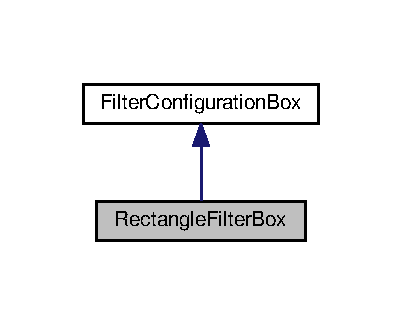
\includegraphics[width=193pt]{classGUI_1_1RectangleFilterBox__inherit__graph}
\end{center}
\end{figure}
\subsection*{Public Member Functions}
\begin{DoxyCompactItemize}
\item 
\hyperlink{classGUI_1_1RectangleFilterBox_ad1d16a75d7930e9f33f867cbed3e5815}{Rectangle\+Filter\+Box} (\hyperlink{classGUI_1_1QWidget}{G\+U\+I\+::\+Q\+Widget} $\ast$parent)
\end{DoxyCompactItemize}
\subsection*{Additional Inherited Members}


\subsection{Detailed Description}
This class contains the gui elements for changing the options of a rectangle filter. 

\subsection{Constructor \& Destructor Documentation}
\hypertarget{classGUI_1_1RectangleFilterBox_ad1d16a75d7930e9f33f867cbed3e5815}{}\index{G\+U\+I\+::\+Rectangle\+Filter\+Box@{G\+U\+I\+::\+Rectangle\+Filter\+Box}!Rectangle\+Filter\+Box@{Rectangle\+Filter\+Box}}
\index{Rectangle\+Filter\+Box@{Rectangle\+Filter\+Box}!G\+U\+I\+::\+Rectangle\+Filter\+Box@{G\+U\+I\+::\+Rectangle\+Filter\+Box}}
\subsubsection[{Rectangle\+Filter\+Box}]{\setlength{\rightskip}{0pt plus 5cm}{\bf Rectangle\+Filter\+Box} (
\begin{DoxyParamCaption}
\item[{{\bf G\+U\+I\+::\+Q\+Widget} $\ast$}]{parent}
\end{DoxyParamCaption}
)}\label{classGUI_1_1RectangleFilterBox_ad1d16a75d7930e9f33f867cbed3e5815}


Constructor. 


\newpage\hypertarget{classUndoRedo_1_1RemoveFilter}{}\section{Remove\+Filter Class Reference}
\label{classUndoRedo_1_1RemoveFilter}\index{Remove\+Filter@{Remove\+Filter}}
\subsection*{Public Member Functions}
\begin{DoxyCompactItemize}
\item 
\hyperlink{classUndoRedo_1_1RemoveFilter_aa60137fea84a032cdc25fe1278b3617e}{Remove\+Filter} (\hyperlink{classGUI_1_1FilterTab}{G\+U\+I\+::\+Filter\+Tab} $\ast$filter\+Tab, \hyperlink{classModel_1_1Filter_1_1Filter}{Model\+::\+Filter\+::\+Filter} filter, int index)
\item 
void \hyperlink{classUndoRedo_1_1RemoveFilter_a0e1e7804a53f6d62efc72c9bdbec8571}{undo} ()
\item 
void \hyperlink{classUndoRedo_1_1RemoveFilter_a93c48d6ed036e1a381be53ac67643284}{redo} ()
\end{DoxyCompactItemize}


\subsection{Detailed Description}
This class is the undo command for removing a filter in the filterlist on the filtertab. 

\subsection{Constructor \& Destructor Documentation}
\hypertarget{classUndoRedo_1_1RemoveFilter_aa60137fea84a032cdc25fe1278b3617e}{}\index{Undo\+Redo\+::\+Remove\+Filter@{Undo\+Redo\+::\+Remove\+Filter}!Remove\+Filter@{Remove\+Filter}}
\index{Remove\+Filter@{Remove\+Filter}!Undo\+Redo\+::\+Remove\+Filter@{Undo\+Redo\+::\+Remove\+Filter}}
\subsubsection[{Remove\+Filter}]{\setlength{\rightskip}{0pt plus 5cm}{\bf Remove\+Filter} (
\begin{DoxyParamCaption}
\item[{{\bf G\+U\+I\+::\+Filter\+Tab} $\ast$}]{filter\+Tab, }
\item[{{\bf Model\+::\+Filter\+::\+Filter}}]{filter, }
\item[{int}]{index}
\end{DoxyParamCaption}
)}\label{classUndoRedo_1_1RemoveFilter_aa60137fea84a032cdc25fe1278b3617e}


Constructor. 


\begin{DoxyParams}{Parameters}
{\em filter\+Tab} & The filtertab to operate on.\\
\hline
{\em filter} & The filter to remove.\\
\hline
{\em index} & The current index of the filter to remove.\\
\hline
\end{DoxyParams}


\subsection{Member Function Documentation}
\hypertarget{classUndoRedo_1_1RemoveFilter_a93c48d6ed036e1a381be53ac67643284}{}\index{Undo\+Redo\+::\+Remove\+Filter@{Undo\+Redo\+::\+Remove\+Filter}!redo@{redo}}
\index{redo@{redo}!Undo\+Redo\+::\+Remove\+Filter@{Undo\+Redo\+::\+Remove\+Filter}}
\subsubsection[{redo}]{\setlength{\rightskip}{0pt plus 5cm}void redo (
\begin{DoxyParamCaption}
{}
\end{DoxyParamCaption}
)}\label{classUndoRedo_1_1RemoveFilter_a93c48d6ed036e1a381be53ac67643284}


Removes a filter from the filterlist. 

\hypertarget{classUndoRedo_1_1RemoveFilter_a0e1e7804a53f6d62efc72c9bdbec8571}{}\index{Undo\+Redo\+::\+Remove\+Filter@{Undo\+Redo\+::\+Remove\+Filter}!undo@{undo}}
\index{undo@{undo}!Undo\+Redo\+::\+Remove\+Filter@{Undo\+Redo\+::\+Remove\+Filter}}
\subsubsection[{undo}]{\setlength{\rightskip}{0pt plus 5cm}void undo (
\begin{DoxyParamCaption}
{}
\end{DoxyParamCaption}
)}\label{classUndoRedo_1_1RemoveFilter_a0e1e7804a53f6d62efc72c9bdbec8571}


Adds the removed filter back into the filterlist. 


\newpage\hypertarget{classUndoRedo_1_1RemoveVideo}{}\section{Remove\+Video Class Reference}
\label{classUndoRedo_1_1RemoveVideo}\index{Remove\+Video@{Remove\+Video}}


Inheritance diagram for Remove\+Video\+:
\nopagebreak
\begin{figure}[H]
\begin{center}
\leavevmode
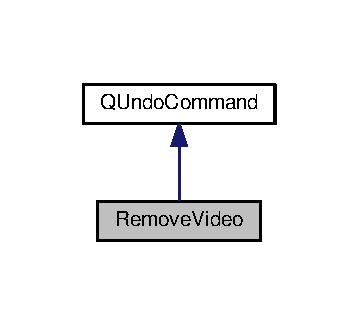
\includegraphics[width=172pt]{classUndoRedo_1_1RemoveVideo__inherit__graph}
\end{center}
\end{figure}
\subsection*{Public Member Functions}
\begin{DoxyCompactItemize}
\item 
\hyperlink{classUndoRedo_1_1RemoveVideo_acb8f85461d6666ff4af154b6018c4cf3}{Remove\+Video} (\hyperlink{classGUI_1_1AnalysisBoxContainer}{G\+U\+I\+::\+Analysis\+Box\+Container} $\ast$container, encoded\+Video \hyperlink{classUndoRedo_1_1RemoveVideo_a226620d1252c162814ca98d3e522255c}{video})
\item 
void \hyperlink{classUndoRedo_1_1RemoveVideo_a0e1e7804a53f6d62efc72c9bdbec8571}{undo} ()
\item 
void \hyperlink{classUndoRedo_1_1RemoveVideo_a93c48d6ed036e1a381be53ac67643284}{redo} ()
\end{DoxyCompactItemize}
\subsection*{Private Attributes}
\begin{DoxyCompactItemize}
\item 
\hyperlink{classGUI_1_1AnalysisBox}{G\+U\+I\+::\+Analysis\+Box} $\ast$ \hyperlink{classUndoRedo_1_1RemoveVideo_a574e9e2f540b9068b64a7f26cb40b20a}{ana\+Box}
\item 
\hyperlink{classGUI_1_1AnalysisBoxContainer}{G\+U\+I\+::\+Analysis\+Box\+Container} $\ast$ \hyperlink{classUndoRedo_1_1RemoveVideo_a69c99d1253a1b743455a030de5a733cb}{ana\+Box\+Container}
\item 
\hyperlink{classModel_1_1EncodedVideo}{Model\+::\+Encoded\+Video} $\ast$ \hyperlink{classUndoRedo_1_1RemoveVideo_a226620d1252c162814ca98d3e522255c}{video}
\end{DoxyCompactItemize}


\subsection{Detailed Description}
This class is the undo command for removing a encoded video in the analysis tab. 

\subsection{Constructor \& Destructor Documentation}
\hypertarget{classUndoRedo_1_1RemoveVideo_acb8f85461d6666ff4af154b6018c4cf3}{}\index{Undo\+Redo\+::\+Remove\+Video@{Undo\+Redo\+::\+Remove\+Video}!Remove\+Video@{Remove\+Video}}
\index{Remove\+Video@{Remove\+Video}!Undo\+Redo\+::\+Remove\+Video@{Undo\+Redo\+::\+Remove\+Video}}
\subsubsection[{Remove\+Video}]{\setlength{\rightskip}{0pt plus 5cm}{\bf Remove\+Video} (
\begin{DoxyParamCaption}
\item[{{\bf G\+U\+I\+::\+Analysis\+Box\+Container} $\ast$}]{container, }
\item[{encoded\+Video}]{video}
\end{DoxyParamCaption}
)}\label{classUndoRedo_1_1RemoveVideo_acb8f85461d6666ff4af154b6018c4cf3}


Constructor. 


\begin{DoxyParams}{Parameters}
{\em container} & The Analysis\+Box\+Container to operate on.\\
\hline
{\em video} & The video to remove.\\
\hline
\end{DoxyParams}


\subsection{Member Function Documentation}
\hypertarget{classUndoRedo_1_1RemoveVideo_a93c48d6ed036e1a381be53ac67643284}{}\index{Undo\+Redo\+::\+Remove\+Video@{Undo\+Redo\+::\+Remove\+Video}!redo@{redo}}
\index{redo@{redo}!Undo\+Redo\+::\+Remove\+Video@{Undo\+Redo\+::\+Remove\+Video}}
\subsubsection[{redo}]{\setlength{\rightskip}{0pt plus 5cm}void redo (
\begin{DoxyParamCaption}
{}
\end{DoxyParamCaption}
)}\label{classUndoRedo_1_1RemoveVideo_a93c48d6ed036e1a381be53ac67643284}


Removes a video from the analysis tab. 

\hypertarget{classUndoRedo_1_1RemoveVideo_a0e1e7804a53f6d62efc72c9bdbec8571}{}\index{Undo\+Redo\+::\+Remove\+Video@{Undo\+Redo\+::\+Remove\+Video}!undo@{undo}}
\index{undo@{undo}!Undo\+Redo\+::\+Remove\+Video@{Undo\+Redo\+::\+Remove\+Video}}
\subsubsection[{undo}]{\setlength{\rightskip}{0pt plus 5cm}void undo (
\begin{DoxyParamCaption}
{}
\end{DoxyParamCaption}
)}\label{classUndoRedo_1_1RemoveVideo_a0e1e7804a53f6d62efc72c9bdbec8571}


Re adds the removed video to the analysis tab. 



\subsection{Field Documentation}
\hypertarget{classUndoRedo_1_1RemoveVideo_a574e9e2f540b9068b64a7f26cb40b20a}{}\index{Undo\+Redo\+::\+Remove\+Video@{Undo\+Redo\+::\+Remove\+Video}!ana\+Box@{ana\+Box}}
\index{ana\+Box@{ana\+Box}!Undo\+Redo\+::\+Remove\+Video@{Undo\+Redo\+::\+Remove\+Video}}
\subsubsection[{ana\+Box}]{\setlength{\rightskip}{0pt plus 5cm}{\bf G\+U\+I\+::\+Analysis\+Box}$\ast$ ana\+Box\hspace{0.3cm}{\ttfamily [private]}}\label{classUndoRedo_1_1RemoveVideo_a574e9e2f540b9068b64a7f26cb40b20a}
\hypertarget{classUndoRedo_1_1RemoveVideo_a69c99d1253a1b743455a030de5a733cb}{}\index{Undo\+Redo\+::\+Remove\+Video@{Undo\+Redo\+::\+Remove\+Video}!ana\+Box\+Container@{ana\+Box\+Container}}
\index{ana\+Box\+Container@{ana\+Box\+Container}!Undo\+Redo\+::\+Remove\+Video@{Undo\+Redo\+::\+Remove\+Video}}
\subsubsection[{ana\+Box\+Container}]{\setlength{\rightskip}{0pt plus 5cm}{\bf G\+U\+I\+::\+Analysis\+Box\+Container}$\ast$ ana\+Box\+Container\hspace{0.3cm}{\ttfamily [private]}}\label{classUndoRedo_1_1RemoveVideo_a69c99d1253a1b743455a030de5a733cb}
\hypertarget{classUndoRedo_1_1RemoveVideo_a226620d1252c162814ca98d3e522255c}{}\index{Undo\+Redo\+::\+Remove\+Video@{Undo\+Redo\+::\+Remove\+Video}!video@{video}}
\index{video@{video}!Undo\+Redo\+::\+Remove\+Video@{Undo\+Redo\+::\+Remove\+Video}}
\subsubsection[{video}]{\setlength{\rightskip}{0pt plus 5cm}{\bf Model\+::\+Encoded\+Video}$\ast$ video\hspace{0.3cm}{\ttfamily [private]}}\label{classUndoRedo_1_1RemoveVideo_a226620d1252c162814ca98d3e522255c}

\newpage\hypertarget{classUtility_1_1RGBDifferenceCalculator}{}\section{R\+G\+B\+Difference\+Calculator Class Reference}
\label{classUtility_1_1RGBDifferenceCalculator}\index{R\+G\+B\+Difference\+Calculator@{R\+G\+B\+Difference\+Calculator}}
\subsection*{Public Member Functions}
\begin{DoxyCompactItemize}
\item 
\hyperlink{classUtility_1_1RGBDifferenceCalculator_a769aad3f6a88d97f35f9eebfe763ee62}{R\+G\+B\+Difference\+Calculator} (\hyperlink{classGUI_1_1Player_1_1Video}{G\+U\+I\+::\+Player\+::\+Video} \&reference\+Video, \hyperlink{classGUI_1_1Player_1_1Video}{G\+U\+I\+::\+Player\+::\+Video} \&video)
\item 
void \hyperlink{classUtility_1_1RGBDifferenceCalculator_aaef52f95d194e2562f5909346428ba04}{calculate\+Video} (\hyperlink{classGUI_1_1Player_1_1Video}{G\+U\+I\+::\+Player\+::\+Video} \&target)
\end{DoxyCompactItemize}


\subsection{Detailed Description}
This class calculates the R\+G\+B-\/difference video of a video. 

\subsection{Constructor \& Destructor Documentation}
\hypertarget{classUtility_1_1RGBDifferenceCalculator_a769aad3f6a88d97f35f9eebfe763ee62}{}\index{Utility\+::\+R\+G\+B\+Difference\+Calculator@{Utility\+::\+R\+G\+B\+Difference\+Calculator}!R\+G\+B\+Difference\+Calculator@{R\+G\+B\+Difference\+Calculator}}
\index{R\+G\+B\+Difference\+Calculator@{R\+G\+B\+Difference\+Calculator}!Utility\+::\+R\+G\+B\+Difference\+Calculator@{Utility\+::\+R\+G\+B\+Difference\+Calculator}}
\subsubsection[{R\+G\+B\+Difference\+Calculator}]{\setlength{\rightskip}{0pt plus 5cm}{\bf R\+G\+B\+Difference\+Calculator} (
\begin{DoxyParamCaption}
\item[{{\bf G\+U\+I\+::\+Player\+::\+Video} \&}]{reference\+Video, }
\item[{{\bf G\+U\+I\+::\+Player\+::\+Video} \&}]{video}
\end{DoxyParamCaption}
)}\label{classUtility_1_1RGBDifferenceCalculator_a769aad3f6a88d97f35f9eebfe763ee62}


Constructor. 


\begin{DoxyParams}{Parameters}
{\em reference\+Video} & The reference video.\\
\hline
{\em video} & The video that is compared to the reference video.\\
\hline
\end{DoxyParams}


\subsection{Member Function Documentation}
\hypertarget{classUtility_1_1RGBDifferenceCalculator_aaef52f95d194e2562f5909346428ba04}{}\index{Utility\+::\+R\+G\+B\+Difference\+Calculator@{Utility\+::\+R\+G\+B\+Difference\+Calculator}!calculate\+Video@{calculate\+Video}}
\index{calculate\+Video@{calculate\+Video}!Utility\+::\+R\+G\+B\+Difference\+Calculator@{Utility\+::\+R\+G\+B\+Difference\+Calculator}}
\subsubsection[{calculate\+Video}]{\setlength{\rightskip}{0pt plus 5cm}void calculate\+Video (
\begin{DoxyParamCaption}
\item[{{\bf G\+U\+I\+::\+Player\+::\+Video} \&}]{target}
\end{DoxyParamCaption}
)}\label{classUtility_1_1RGBDifferenceCalculator_aaef52f95d194e2562f5909346428ba04}


Calculates the R\+G\+B difference between two videos. 


\begin{DoxyParams}{Parameters}
{\em target} & the video the calculated frames are added to\\
\hline
\end{DoxyParams}

\newpage\hypertarget{classModel_1_1RGBFilter}{}\section{R\+G\+B\+Filter Class Reference}
\label{classModel_1_1RGBFilter}\index{R\+G\+B\+Filter@{R\+G\+B\+Filter}}


Inheritance diagram for R\+G\+B\+Filter\+:
\nopagebreak
\begin{figure}[H]
\begin{center}
\leavevmode
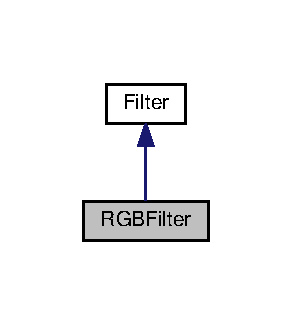
\includegraphics[width=140pt]{classModel_1_1RGBFilter__inherit__graph}
\end{center}
\end{figure}
\subsection*{Public Member Functions}
\begin{DoxyCompactItemize}
\item 
\hyperlink{classModel_1_1RGBFilter_a9065d7c86503c630a3422f5db4af723f}{R\+G\+B\+Filter} ()
\item 
string \hyperlink{classModel_1_1RGBFilter_a62b7b60e24f92234393b840b35808e06}{get\+Filter\+Description} ()
\item 
\hyperlink{namespaceModel_a54742b2fc8f6a246926cbb87b7fae1a4}{Model\+::\+Basic\+Color} \hyperlink{classModel_1_1RGBFilter_a82ac188d01a7ce771cdb254e9eb70ba6}{get\+Color} ()
\item 
void \hyperlink{classModel_1_1RGBFilter_a707221b518c3ae5bf8ce16cc9b0d0054}{set\+Color} (\hyperlink{namespaceModel_a54742b2fc8f6a246926cbb87b7fae1a4}{Model\+::\+Basic\+Color} \hyperlink{classModel_1_1RGBFilter_af9c4a828f1030ef2b7d7ab814dd37cb9}{color})
\item 
string \hyperlink{classModel_1_1RGBFilter_a11335e13e50af74108bf926dc1340b4b}{get\+Name} ()
\end{DoxyCompactItemize}
\subsection*{Private Attributes}
\begin{DoxyCompactItemize}
\item 
\hyperlink{namespaceModel_a54742b2fc8f6a246926cbb87b7fae1a4}{Model\+::\+Basic\+Color} $\ast$ \hyperlink{classModel_1_1RGBFilter_af9c4a828f1030ef2b7d7ab814dd37cb9}{color}
\end{DoxyCompactItemize}
\subsection*{Additional Inherited Members}


\subsection{Detailed Description}
Filters the video by a given channel (red, green or blue). 

\subsection{Constructor \& Destructor Documentation}
\hypertarget{classModel_1_1RGBFilter_a9065d7c86503c630a3422f5db4af723f}{}\index{Model\+::\+R\+G\+B\+Filter@{Model\+::\+R\+G\+B\+Filter}!R\+G\+B\+Filter@{R\+G\+B\+Filter}}
\index{R\+G\+B\+Filter@{R\+G\+B\+Filter}!Model\+::\+R\+G\+B\+Filter@{Model\+::\+R\+G\+B\+Filter}}
\subsubsection[{R\+G\+B\+Filter}]{\setlength{\rightskip}{0pt plus 5cm}{\bf R\+G\+B\+Filter} (
\begin{DoxyParamCaption}
{}
\end{DoxyParamCaption}
)}\label{classModel_1_1RGBFilter_a9065d7c86503c630a3422f5db4af723f}


Constructor. 



\subsection{Member Function Documentation}
\hypertarget{classModel_1_1RGBFilter_a82ac188d01a7ce771cdb254e9eb70ba6}{}\index{Model\+::\+R\+G\+B\+Filter@{Model\+::\+R\+G\+B\+Filter}!get\+Color@{get\+Color}}
\index{get\+Color@{get\+Color}!Model\+::\+R\+G\+B\+Filter@{Model\+::\+R\+G\+B\+Filter}}
\subsubsection[{get\+Color}]{\setlength{\rightskip}{0pt plus 5cm}{\bf Model\+::\+Basic\+Color} get\+Color (
\begin{DoxyParamCaption}
{}
\end{DoxyParamCaption}
)}\label{classModel_1_1RGBFilter_a82ac188d01a7ce771cdb254e9eb70ba6}


Returns the color that is not filtered out. 

\begin{DoxyReturn}{Returns}
The preserved color.
\end{DoxyReturn}
\hypertarget{classModel_1_1RGBFilter_a62b7b60e24f92234393b840b35808e06}{}\index{Model\+::\+R\+G\+B\+Filter@{Model\+::\+R\+G\+B\+Filter}!get\+Filter\+Description@{get\+Filter\+Description}}
\index{get\+Filter\+Description@{get\+Filter\+Description}!Model\+::\+R\+G\+B\+Filter@{Model\+::\+R\+G\+B\+Filter}}
\subsubsection[{get\+Filter\+Description}]{\setlength{\rightskip}{0pt plus 5cm}string get\+Filter\+Description (
\begin{DoxyParamCaption}
{}
\end{DoxyParamCaption}
)\hspace{0.3cm}{\ttfamily [virtual]}}\label{classModel_1_1RGBFilter_a62b7b60e24f92234393b840b35808e06}


Returns the string that the ffmpeg library needs to apply the filter to a video. 

\begin{DoxyReturn}{Returns}
The string for the ffmpeg library.
\end{DoxyReturn}


Implements \hyperlink{classModel_1_1Filter_a453fcafa809afa1ce58d9ef95d5f26c0}{Filter}.

\hypertarget{classModel_1_1RGBFilter_a11335e13e50af74108bf926dc1340b4b}{}\index{Model\+::\+R\+G\+B\+Filter@{Model\+::\+R\+G\+B\+Filter}!get\+Name@{get\+Name}}
\index{get\+Name@{get\+Name}!Model\+::\+R\+G\+B\+Filter@{Model\+::\+R\+G\+B\+Filter}}
\subsubsection[{get\+Name}]{\setlength{\rightskip}{0pt plus 5cm}string get\+Name (
\begin{DoxyParamCaption}
{}
\end{DoxyParamCaption}
)\hspace{0.3cm}{\ttfamily [virtual]}}\label{classModel_1_1RGBFilter_a11335e13e50af74108bf926dc1340b4b}


Returns the name of the filter. 

\begin{DoxyReturn}{Returns}
The filtername.
\end{DoxyReturn}


Implements \hyperlink{classModel_1_1Filter_ade93aa98c68d185a9c03784d36140225}{Filter}.

\hypertarget{classModel_1_1RGBFilter_a707221b518c3ae5bf8ce16cc9b0d0054}{}\index{Model\+::\+R\+G\+B\+Filter@{Model\+::\+R\+G\+B\+Filter}!set\+Color@{set\+Color}}
\index{set\+Color@{set\+Color}!Model\+::\+R\+G\+B\+Filter@{Model\+::\+R\+G\+B\+Filter}}
\subsubsection[{set\+Color}]{\setlength{\rightskip}{0pt plus 5cm}void set\+Color (
\begin{DoxyParamCaption}
\item[{{\bf Model\+::\+Basic\+Color}}]{color}
\end{DoxyParamCaption}
)}\label{classModel_1_1RGBFilter_a707221b518c3ae5bf8ce16cc9b0d0054}


Sets the preserved color. 


\begin{DoxyParams}{Parameters}
{\em color} & The preserved color.\\
\hline
\end{DoxyParams}


\subsection{Field Documentation}
\hypertarget{classModel_1_1RGBFilter_af9c4a828f1030ef2b7d7ab814dd37cb9}{}\index{Model\+::\+R\+G\+B\+Filter@{Model\+::\+R\+G\+B\+Filter}!color@{color}}
\index{color@{color}!Model\+::\+R\+G\+B\+Filter@{Model\+::\+R\+G\+B\+Filter}}
\subsubsection[{color}]{\setlength{\rightskip}{0pt plus 5cm}{\bf Model\+::\+Basic\+Color}$\ast$ color\hspace{0.3cm}{\ttfamily [private]}}\label{classModel_1_1RGBFilter_af9c4a828f1030ef2b7d7ab814dd37cb9}

\newpage\hypertarget{classGUI_1_1RGBFilterBox}{}\section{R\+G\+B\+Filter\+Box Class Reference}
\label{classGUI_1_1RGBFilterBox}\index{R\+G\+B\+Filter\+Box@{R\+G\+B\+Filter\+Box}}
\subsection*{Public Member Functions}
\begin{DoxyCompactItemize}
\item 
\hyperlink{classGUI_1_1RGBFilterBox_a2bd622e6f8727ea01b985e13e407d6ac}{R\+G\+B\+Filter\+Box} (\hyperlink{classGUI_1_1Player_1_1QWidget}{G\+U\+I\+::\+Player\+::\+Q\+Widget} $\ast$parent)
\end{DoxyCompactItemize}
\subsection*{Additional Inherited Members}


\subsection{Detailed Description}
This class contains the gui elements for changing the options of a rgb filter. 

\subsection{Constructor \& Destructor Documentation}
\hypertarget{classGUI_1_1RGBFilterBox_a2bd622e6f8727ea01b985e13e407d6ac}{}\index{G\+U\+I\+::\+R\+G\+B\+Filter\+Box@{G\+U\+I\+::\+R\+G\+B\+Filter\+Box}!R\+G\+B\+Filter\+Box@{R\+G\+B\+Filter\+Box}}
\index{R\+G\+B\+Filter\+Box@{R\+G\+B\+Filter\+Box}!G\+U\+I\+::\+R\+G\+B\+Filter\+Box@{G\+U\+I\+::\+R\+G\+B\+Filter\+Box}}
\subsubsection[{R\+G\+B\+Filter\+Box}]{\setlength{\rightskip}{0pt plus 5cm}{\bf R\+G\+B\+Filter\+Box} (
\begin{DoxyParamCaption}
\item[{{\bf G\+U\+I\+::\+Player\+::\+Q\+Widget} $\ast$}]{parent}
\end{DoxyParamCaption}
)}\label{classGUI_1_1RGBFilterBox_a2bd622e6f8727ea01b985e13e407d6ac}


Constructor. 


\newpage\hypertarget{classUtility_1_1RGBHistogrammCalculator}{}\section{R\+G\+B\+Histogramm\+Calculator Class Reference}
\label{classUtility_1_1RGBHistogrammCalculator}\index{R\+G\+B\+Histogramm\+Calculator@{R\+G\+B\+Histogramm\+Calculator}}
\subsection*{Public Member Functions}
\begin{DoxyCompactItemize}
\item 
void \hyperlink{classUtility_1_1RGBHistogrammCalculator_a0c01f44967ccf0d367f88a1bfd72c701}{R\+G\+B\+Historgramm\+Calculator} (\hyperlink{classGUI_1_1Player_1_1Video}{G\+U\+I\+::\+Player\+::\+Video} \&video)
\item 
void \hyperlink{classUtility_1_1RGBHistogrammCalculator_afe1d8348c24e6589bc7c0b3f689316a7}{calculate} ()
\item 
\hyperlink{classModel_1_1Graph}{Model\+::\+Graph} \hyperlink{classUtility_1_1RGBHistogrammCalculator_a11345d1b2b32275950a10525c1e0e9d1}{get\+Red\+Histogramm} ()
\item 
\hyperlink{classModel_1_1Graph}{Model\+::\+Graph} \hyperlink{classUtility_1_1RGBHistogrammCalculator_a84bbb0085709b08aef6f9f2a849dcf10}{get\+Green\+Histogramm} ()
\item 
\hyperlink{classModel_1_1Graph}{Model\+::\+Graph} \hyperlink{classUtility_1_1RGBHistogrammCalculator_a6bc6a7ac3d5da8080b9c5f146c0d4e8f}{get\+Blue\+Histogramm} ()
\end{DoxyCompactItemize}


\subsection{Detailed Description}
This class calculates the R\+G\+B histogramm for a video. 

\subsection{Member Function Documentation}
\hypertarget{classUtility_1_1RGBHistogrammCalculator_afe1d8348c24e6589bc7c0b3f689316a7}{}\index{Utility\+::\+R\+G\+B\+Histogramm\+Calculator@{Utility\+::\+R\+G\+B\+Histogramm\+Calculator}!calculate@{calculate}}
\index{calculate@{calculate}!Utility\+::\+R\+G\+B\+Histogramm\+Calculator@{Utility\+::\+R\+G\+B\+Histogramm\+Calculator}}
\subsubsection[{calculate}]{\setlength{\rightskip}{0pt plus 5cm}void calculate (
\begin{DoxyParamCaption}
{}
\end{DoxyParamCaption}
)}\label{classUtility_1_1RGBHistogrammCalculator_afe1d8348c24e6589bc7c0b3f689316a7}


Calculates the red, green and blue components of a video. 

\hypertarget{classUtility_1_1RGBHistogrammCalculator_a6bc6a7ac3d5da8080b9c5f146c0d4e8f}{}\index{Utility\+::\+R\+G\+B\+Histogramm\+Calculator@{Utility\+::\+R\+G\+B\+Histogramm\+Calculator}!get\+Blue\+Histogramm@{get\+Blue\+Histogramm}}
\index{get\+Blue\+Histogramm@{get\+Blue\+Histogramm}!Utility\+::\+R\+G\+B\+Histogramm\+Calculator@{Utility\+::\+R\+G\+B\+Histogramm\+Calculator}}
\subsubsection[{get\+Blue\+Histogramm}]{\setlength{\rightskip}{0pt plus 5cm}{\bf Model\+::\+Graph} get\+Blue\+Histogramm (
\begin{DoxyParamCaption}
{}
\end{DoxyParamCaption}
)}\label{classUtility_1_1RGBHistogrammCalculator_a6bc6a7ac3d5da8080b9c5f146c0d4e8f}


Returns the blue components of a video. 

\hypertarget{classUtility_1_1RGBHistogrammCalculator_a84bbb0085709b08aef6f9f2a849dcf10}{}\index{Utility\+::\+R\+G\+B\+Histogramm\+Calculator@{Utility\+::\+R\+G\+B\+Histogramm\+Calculator}!get\+Green\+Histogramm@{get\+Green\+Histogramm}}
\index{get\+Green\+Histogramm@{get\+Green\+Histogramm}!Utility\+::\+R\+G\+B\+Histogramm\+Calculator@{Utility\+::\+R\+G\+B\+Histogramm\+Calculator}}
\subsubsection[{get\+Green\+Histogramm}]{\setlength{\rightskip}{0pt plus 5cm}{\bf Model\+::\+Graph} get\+Green\+Histogramm (
\begin{DoxyParamCaption}
{}
\end{DoxyParamCaption}
)}\label{classUtility_1_1RGBHistogrammCalculator_a84bbb0085709b08aef6f9f2a849dcf10}


Returns the green components of a video. 

\hypertarget{classUtility_1_1RGBHistogrammCalculator_a11345d1b2b32275950a10525c1e0e9d1}{}\index{Utility\+::\+R\+G\+B\+Histogramm\+Calculator@{Utility\+::\+R\+G\+B\+Histogramm\+Calculator}!get\+Red\+Histogramm@{get\+Red\+Histogramm}}
\index{get\+Red\+Histogramm@{get\+Red\+Histogramm}!Utility\+::\+R\+G\+B\+Histogramm\+Calculator@{Utility\+::\+R\+G\+B\+Histogramm\+Calculator}}
\subsubsection[{get\+Red\+Histogramm}]{\setlength{\rightskip}{0pt plus 5cm}{\bf Model\+::\+Graph} get\+Red\+Histogramm (
\begin{DoxyParamCaption}
{}
\end{DoxyParamCaption}
)}\label{classUtility_1_1RGBHistogrammCalculator_a11345d1b2b32275950a10525c1e0e9d1}


Returns the red components of a video. 

\hypertarget{classUtility_1_1RGBHistogrammCalculator_a0c01f44967ccf0d367f88a1bfd72c701}{}\index{Utility\+::\+R\+G\+B\+Histogramm\+Calculator@{Utility\+::\+R\+G\+B\+Histogramm\+Calculator}!R\+G\+B\+Historgramm\+Calculator@{R\+G\+B\+Historgramm\+Calculator}}
\index{R\+G\+B\+Historgramm\+Calculator@{R\+G\+B\+Historgramm\+Calculator}!Utility\+::\+R\+G\+B\+Histogramm\+Calculator@{Utility\+::\+R\+G\+B\+Histogramm\+Calculator}}
\subsubsection[{R\+G\+B\+Historgramm\+Calculator}]{\setlength{\rightskip}{0pt plus 5cm}void R\+G\+B\+Historgramm\+Calculator (
\begin{DoxyParamCaption}
\item[{{\bf G\+U\+I\+::\+Player\+::\+Video} \&}]{video}
\end{DoxyParamCaption}
)}\label{classUtility_1_1RGBHistogrammCalculator_a0c01f44967ccf0d367f88a1bfd72c701}


Constructor. 


\begin{DoxyParams}{Parameters}
{\em video} & the video that is analyzed.\\
\hline
\end{DoxyParams}

\newpage\hypertarget{classModel_1_1RotationFilter}{}\section{Rotation\+Filter Class Reference}
\label{classModel_1_1RotationFilter}\index{Rotation\+Filter@{Rotation\+Filter}}


Inheritance diagram for Rotation\+Filter\+:
\nopagebreak
\begin{figure}[H]
\begin{center}
\leavevmode
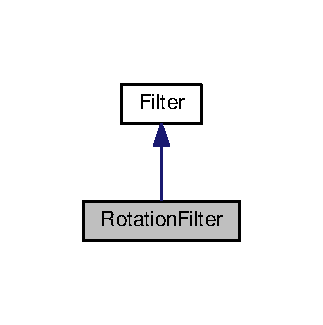
\includegraphics[width=155pt]{classModel_1_1RotationFilter__inherit__graph}
\end{center}
\end{figure}
\subsection*{Public Member Functions}
\begin{DoxyCompactItemize}
\item 
\hyperlink{classModel_1_1RotationFilter_a81e4560ff6f30e689b915149f4db871c}{Rotation\+Filter} ()
\item 
string \hyperlink{classModel_1_1RotationFilter_a62b7b60e24f92234393b840b35808e06}{get\+Filter\+Description} ()
\item 
int \hyperlink{classModel_1_1RotationFilter_ae71094a2b50726fbec9d9475b2c92e01}{get\+Angle} ()
\item 
string \hyperlink{classModel_1_1RotationFilter_a11335e13e50af74108bf926dc1340b4b}{get\+Name} ()
\item 
void \hyperlink{classModel_1_1RotationFilter_a241a28cb2a44be5be3440363436be22f}{set\+Angle} (int \hyperlink{classModel_1_1RotationFilter_a63177970cacb40efba67ce501ea89210}{angle})
\end{DoxyCompactItemize}
\subsection*{Private Attributes}
\begin{DoxyCompactItemize}
\item 
int \hyperlink{classModel_1_1RotationFilter_a63177970cacb40efba67ce501ea89210}{angle}
\end{DoxyCompactItemize}
\subsection*{Additional Inherited Members}


\subsection{Detailed Description}
Rotates the video. 

\subsection{Constructor \& Destructor Documentation}
\hypertarget{classModel_1_1RotationFilter_a81e4560ff6f30e689b915149f4db871c}{}\index{Model\+::\+Rotation\+Filter@{Model\+::\+Rotation\+Filter}!Rotation\+Filter@{Rotation\+Filter}}
\index{Rotation\+Filter@{Rotation\+Filter}!Model\+::\+Rotation\+Filter@{Model\+::\+Rotation\+Filter}}
\subsubsection[{Rotation\+Filter}]{\setlength{\rightskip}{0pt plus 5cm}{\bf Rotation\+Filter} (
\begin{DoxyParamCaption}
{}
\end{DoxyParamCaption}
)}\label{classModel_1_1RotationFilter_a81e4560ff6f30e689b915149f4db871c}


Constructor. 



\subsection{Member Function Documentation}
\hypertarget{classModel_1_1RotationFilter_ae71094a2b50726fbec9d9475b2c92e01}{}\index{Model\+::\+Rotation\+Filter@{Model\+::\+Rotation\+Filter}!get\+Angle@{get\+Angle}}
\index{get\+Angle@{get\+Angle}!Model\+::\+Rotation\+Filter@{Model\+::\+Rotation\+Filter}}
\subsubsection[{get\+Angle}]{\setlength{\rightskip}{0pt plus 5cm}int get\+Angle (
\begin{DoxyParamCaption}
{}
\end{DoxyParamCaption}
)}\label{classModel_1_1RotationFilter_ae71094a2b50726fbec9d9475b2c92e01}


Returns the angle of the rotation. 

\begin{DoxyReturn}{Returns}
The rotation angle.
\end{DoxyReturn}
\hypertarget{classModel_1_1RotationFilter_a62b7b60e24f92234393b840b35808e06}{}\index{Model\+::\+Rotation\+Filter@{Model\+::\+Rotation\+Filter}!get\+Filter\+Description@{get\+Filter\+Description}}
\index{get\+Filter\+Description@{get\+Filter\+Description}!Model\+::\+Rotation\+Filter@{Model\+::\+Rotation\+Filter}}
\subsubsection[{get\+Filter\+Description}]{\setlength{\rightskip}{0pt plus 5cm}string get\+Filter\+Description (
\begin{DoxyParamCaption}
{}
\end{DoxyParamCaption}
)\hspace{0.3cm}{\ttfamily [virtual]}}\label{classModel_1_1RotationFilter_a62b7b60e24f92234393b840b35808e06}


Returns the string that the ffmpeg library needs to apply the filter to a video. 

\begin{DoxyReturn}{Returns}
The string for the ffmpeg library.
\end{DoxyReturn}


Implements \hyperlink{classModel_1_1Filter_a453fcafa809afa1ce58d9ef95d5f26c0}{Filter}.

\hypertarget{classModel_1_1RotationFilter_a11335e13e50af74108bf926dc1340b4b}{}\index{Model\+::\+Rotation\+Filter@{Model\+::\+Rotation\+Filter}!get\+Name@{get\+Name}}
\index{get\+Name@{get\+Name}!Model\+::\+Rotation\+Filter@{Model\+::\+Rotation\+Filter}}
\subsubsection[{get\+Name}]{\setlength{\rightskip}{0pt plus 5cm}string get\+Name (
\begin{DoxyParamCaption}
{}
\end{DoxyParamCaption}
)\hspace{0.3cm}{\ttfamily [virtual]}}\label{classModel_1_1RotationFilter_a11335e13e50af74108bf926dc1340b4b}


Returns the name of the filter. 

\begin{DoxyReturn}{Returns}
The filtername.
\end{DoxyReturn}


Implements \hyperlink{classModel_1_1Filter_ade93aa98c68d185a9c03784d36140225}{Filter}.

\hypertarget{classModel_1_1RotationFilter_a241a28cb2a44be5be3440363436be22f}{}\index{Model\+::\+Rotation\+Filter@{Model\+::\+Rotation\+Filter}!set\+Angle@{set\+Angle}}
\index{set\+Angle@{set\+Angle}!Model\+::\+Rotation\+Filter@{Model\+::\+Rotation\+Filter}}
\subsubsection[{set\+Angle}]{\setlength{\rightskip}{0pt plus 5cm}void set\+Angle (
\begin{DoxyParamCaption}
\item[{int}]{angle}
\end{DoxyParamCaption}
)}\label{classModel_1_1RotationFilter_a241a28cb2a44be5be3440363436be22f}


Sets the angle of the rotation. 


\begin{DoxyParams}{Parameters}
{\em angle} & The new rotation angle.\\
\hline
\end{DoxyParams}


\subsection{Field Documentation}
\hypertarget{classModel_1_1RotationFilter_a63177970cacb40efba67ce501ea89210}{}\index{Model\+::\+Rotation\+Filter@{Model\+::\+Rotation\+Filter}!angle@{angle}}
\index{angle@{angle}!Model\+::\+Rotation\+Filter@{Model\+::\+Rotation\+Filter}}
\subsubsection[{angle}]{\setlength{\rightskip}{0pt plus 5cm}int angle\hspace{0.3cm}{\ttfamily [private]}}\label{classModel_1_1RotationFilter_a63177970cacb40efba67ce501ea89210}

\newpage\hypertarget{classGUI_1_1RotationFilterBox}{}\section{Rotation\+Filter\+Box Class Reference}
\label{classGUI_1_1RotationFilterBox}\index{Rotation\+Filter\+Box@{Rotation\+Filter\+Box}}


Inheritance diagram for Rotation\+Filter\+Box\+:
\nopagebreak
\begin{figure}[H]
\begin{center}
\leavevmode
\includegraphics[width=193pt]{classGUI_1_1RotationFilterBox__inherit__graph}
\end{center}
\end{figure}
\subsection*{Public Member Functions}
\begin{DoxyCompactItemize}
\item 
\hyperlink{classGUI_1_1RotationFilterBox_a86a39151a9e0eae3f619853f8469db4e}{Rotation\+Filter\+Box} (\hyperlink{classGUI_1_1QWidget}{G\+U\+I\+::\+Q\+Widget} $\ast$parent)
\end{DoxyCompactItemize}
\subsection*{Additional Inherited Members}


\subsection{Detailed Description}
This class contains the gui elements for changing the options of a rotation filter. 

\subsection{Constructor \& Destructor Documentation}
\hypertarget{classGUI_1_1RotationFilterBox_a86a39151a9e0eae3f619853f8469db4e}{}\index{G\+U\+I\+::\+Rotation\+Filter\+Box@{G\+U\+I\+::\+Rotation\+Filter\+Box}!Rotation\+Filter\+Box@{Rotation\+Filter\+Box}}
\index{Rotation\+Filter\+Box@{Rotation\+Filter\+Box}!G\+U\+I\+::\+Rotation\+Filter\+Box@{G\+U\+I\+::\+Rotation\+Filter\+Box}}
\subsubsection[{Rotation\+Filter\+Box}]{\setlength{\rightskip}{0pt plus 5cm}{\bf Rotation\+Filter\+Box} (
\begin{DoxyParamCaption}
\item[{{\bf G\+U\+I\+::\+Q\+Widget} $\ast$}]{parent}
\end{DoxyParamCaption}
)}\label{classGUI_1_1RotationFilterBox_a86a39151a9e0eae3f619853f8469db4e}


Constructor. 


\newpage\hypertarget{classModel_1_1SaturationFilter}{}\section{Saturation\+Filter Class Reference}
\label{classModel_1_1SaturationFilter}\index{Saturation\+Filter@{Saturation\+Filter}}


Inheritance diagram for Saturation\+Filter\+:
\nopagebreak
\begin{figure}[H]
\begin{center}
\leavevmode
\includegraphics[width=163pt]{classModel_1_1SaturationFilter__inherit__graph}
\end{center}
\end{figure}
\subsection*{Public Member Functions}
\begin{DoxyCompactItemize}
\item 
\hyperlink{classModel_1_1SaturationFilter_ae45fd836bb8ade0550727f4060bdffa9}{Saturation\+Filter} ()
\item 
string \hyperlink{classModel_1_1SaturationFilter_a62b7b60e24f92234393b840b35808e06}{get\+Filter\+Description} ()
\item 
int \hyperlink{classModel_1_1SaturationFilter_a708995fb1b6acb31ee0dfb0f4881e5b5}{get\+Intensity} ()
\item 
string \hyperlink{classModel_1_1SaturationFilter_a11335e13e50af74108bf926dc1340b4b}{get\+Name} ()
\item 
void \hyperlink{classModel_1_1SaturationFilter_ac8255ffbc46bb61acaa8fd23d0d260eb}{set\+Intensity} (int \hyperlink{classModel_1_1SaturationFilter_a299ec0c42ccc5a2d79d1739428ac3210}{intensity})
\end{DoxyCompactItemize}
\subsection*{Private Attributes}
\begin{DoxyCompactItemize}
\item 
int \hyperlink{classModel_1_1SaturationFilter_a299ec0c42ccc5a2d79d1739428ac3210}{intensity}
\end{DoxyCompactItemize}
\subsection*{Additional Inherited Members}


\subsection{Detailed Description}
Adjusts the saturation of the video. 

\subsection{Constructor \& Destructor Documentation}
\hypertarget{classModel_1_1SaturationFilter_ae45fd836bb8ade0550727f4060bdffa9}{}\index{Model\+::\+Saturation\+Filter@{Model\+::\+Saturation\+Filter}!Saturation\+Filter@{Saturation\+Filter}}
\index{Saturation\+Filter@{Saturation\+Filter}!Model\+::\+Saturation\+Filter@{Model\+::\+Saturation\+Filter}}
\subsubsection[{Saturation\+Filter}]{\setlength{\rightskip}{0pt plus 5cm}{\bf Saturation\+Filter} (
\begin{DoxyParamCaption}
{}
\end{DoxyParamCaption}
)}\label{classModel_1_1SaturationFilter_ae45fd836bb8ade0550727f4060bdffa9}


Constructor. 



\subsection{Member Function Documentation}
\hypertarget{classModel_1_1SaturationFilter_a62b7b60e24f92234393b840b35808e06}{}\index{Model\+::\+Saturation\+Filter@{Model\+::\+Saturation\+Filter}!get\+Filter\+Description@{get\+Filter\+Description}}
\index{get\+Filter\+Description@{get\+Filter\+Description}!Model\+::\+Saturation\+Filter@{Model\+::\+Saturation\+Filter}}
\subsubsection[{get\+Filter\+Description}]{\setlength{\rightskip}{0pt plus 5cm}string get\+Filter\+Description (
\begin{DoxyParamCaption}
{}
\end{DoxyParamCaption}
)\hspace{0.3cm}{\ttfamily [virtual]}}\label{classModel_1_1SaturationFilter_a62b7b60e24f92234393b840b35808e06}


Returns the string that the ffmpeg library needs to apply the filter to a video. 

\begin{DoxyReturn}{Returns}
The string for the ffmpeg library.
\end{DoxyReturn}


Implements \hyperlink{classModel_1_1Filter_a453fcafa809afa1ce58d9ef95d5f26c0}{Filter}.

\hypertarget{classModel_1_1SaturationFilter_a708995fb1b6acb31ee0dfb0f4881e5b5}{}\index{Model\+::\+Saturation\+Filter@{Model\+::\+Saturation\+Filter}!get\+Intensity@{get\+Intensity}}
\index{get\+Intensity@{get\+Intensity}!Model\+::\+Saturation\+Filter@{Model\+::\+Saturation\+Filter}}
\subsubsection[{get\+Intensity}]{\setlength{\rightskip}{0pt plus 5cm}int get\+Intensity (
\begin{DoxyParamCaption}
{}
\end{DoxyParamCaption}
)}\label{classModel_1_1SaturationFilter_a708995fb1b6acb31ee0dfb0f4881e5b5}


Returns the intensity of the saturation. 

\begin{DoxyReturn}{Returns}
The intensity.
\end{DoxyReturn}
\hypertarget{classModel_1_1SaturationFilter_a11335e13e50af74108bf926dc1340b4b}{}\index{Model\+::\+Saturation\+Filter@{Model\+::\+Saturation\+Filter}!get\+Name@{get\+Name}}
\index{get\+Name@{get\+Name}!Model\+::\+Saturation\+Filter@{Model\+::\+Saturation\+Filter}}
\subsubsection[{get\+Name}]{\setlength{\rightskip}{0pt plus 5cm}string get\+Name (
\begin{DoxyParamCaption}
{}
\end{DoxyParamCaption}
)\hspace{0.3cm}{\ttfamily [virtual]}}\label{classModel_1_1SaturationFilter_a11335e13e50af74108bf926dc1340b4b}


Returns the name of the filter. 

\begin{DoxyReturn}{Returns}
The filtername.
\end{DoxyReturn}


Implements \hyperlink{classModel_1_1Filter_ade93aa98c68d185a9c03784d36140225}{Filter}.

\hypertarget{classModel_1_1SaturationFilter_ac8255ffbc46bb61acaa8fd23d0d260eb}{}\index{Model\+::\+Saturation\+Filter@{Model\+::\+Saturation\+Filter}!set\+Intensity@{set\+Intensity}}
\index{set\+Intensity@{set\+Intensity}!Model\+::\+Saturation\+Filter@{Model\+::\+Saturation\+Filter}}
\subsubsection[{set\+Intensity}]{\setlength{\rightskip}{0pt plus 5cm}void set\+Intensity (
\begin{DoxyParamCaption}
\item[{int}]{intensity}
\end{DoxyParamCaption}
)}\label{classModel_1_1SaturationFilter_ac8255ffbc46bb61acaa8fd23d0d260eb}


Sets the intensity of the saturation. 


\begin{DoxyParams}{Parameters}
{\em intensity} & The new intensity,\\
\hline
\end{DoxyParams}


\subsection{Field Documentation}
\hypertarget{classModel_1_1SaturationFilter_a299ec0c42ccc5a2d79d1739428ac3210}{}\index{Model\+::\+Saturation\+Filter@{Model\+::\+Saturation\+Filter}!intensity@{intensity}}
\index{intensity@{intensity}!Model\+::\+Saturation\+Filter@{Model\+::\+Saturation\+Filter}}
\subsubsection[{intensity}]{\setlength{\rightskip}{0pt plus 5cm}int intensity\hspace{0.3cm}{\ttfamily [private]}}\label{classModel_1_1SaturationFilter_a299ec0c42ccc5a2d79d1739428ac3210}

\newpage\hypertarget{classGUI_1_1SaturationFilterBox}{}\section{Saturation\+Filter\+Box Class Reference}
\label{classGUI_1_1SaturationFilterBox}\index{Saturation\+Filter\+Box@{Saturation\+Filter\+Box}}


Inheritance diagram for Saturation\+Filter\+Box\+:
\nopagebreak
\begin{figure}[H]
\begin{center}
\leavevmode
\includegraphics[width=193pt]{classGUI_1_1SaturationFilterBox__inherit__graph}
\end{center}
\end{figure}
\subsection*{Public Member Functions}
\begin{DoxyCompactItemize}
\item 
\hyperlink{classGUI_1_1SaturationFilterBox_aedb403a0d62fc7b393637eceb4e7eecb}{Saturation\+Filter\+Box} (\hyperlink{classGUI_1_1QWidget}{G\+U\+I\+::\+Q\+Widget} $\ast$parent)
\end{DoxyCompactItemize}
\subsection*{Additional Inherited Members}


\subsection{Detailed Description}
This class contains the gui elements for changing the options of a saturation filter. 

\subsection{Constructor \& Destructor Documentation}
\hypertarget{classGUI_1_1SaturationFilterBox_aedb403a0d62fc7b393637eceb4e7eecb}{}\index{G\+U\+I\+::\+Saturation\+Filter\+Box@{G\+U\+I\+::\+Saturation\+Filter\+Box}!Saturation\+Filter\+Box@{Saturation\+Filter\+Box}}
\index{Saturation\+Filter\+Box@{Saturation\+Filter\+Box}!G\+U\+I\+::\+Saturation\+Filter\+Box@{G\+U\+I\+::\+Saturation\+Filter\+Box}}
\subsubsection[{Saturation\+Filter\+Box}]{\setlength{\rightskip}{0pt plus 5cm}{\bf Saturation\+Filter\+Box} (
\begin{DoxyParamCaption}
\item[{{\bf G\+U\+I\+::\+Q\+Widget} $\ast$}]{parent}
\end{DoxyParamCaption}
)}\label{classGUI_1_1SaturationFilterBox_aedb403a0d62fc7b393637eceb4e7eecb}


Constructor. 


\newpage\hypertarget{classModel_1_1ScaleFilter}{}\section{Scale\+Filter Class Reference}
\label{classModel_1_1ScaleFilter}\index{Scale\+Filter@{Scale\+Filter}}


Inheritance diagram for Scale\+Filter\+:
\nopagebreak
\begin{figure}[H]
\begin{center}
\leavevmode
\includegraphics[width=143pt]{classModel_1_1ScaleFilter__inherit__graph}
\end{center}
\end{figure}
\subsection*{Public Member Functions}
\begin{DoxyCompactItemize}
\item 
\hyperlink{classModel_1_1ScaleFilter_a97c359581f0dd70601196694efdace5a}{Scale\+Filter} ()
\item 
string \hyperlink{classModel_1_1ScaleFilter_a62b7b60e24f92234393b840b35808e06}{get\+Filter\+Description} ()
\item 
bool \hyperlink{classModel_1_1ScaleFilter_a24f2abc27a0f228db8763dbecb6ad326}{get\+Keep\+Ratio} ()
\item 
void \hyperlink{classModel_1_1ScaleFilter_a8a9a32b92c6a9dc160091d8886ba13dc}{set\+Keep\+Ratio} (bool \hyperlink{classModel_1_1ScaleFilter_a2a8bde298e312d75b2de36f51698a1b1}{keep\+Ratio})
\item 
string \hyperlink{classModel_1_1ScaleFilter_a11335e13e50af74108bf926dc1340b4b}{get\+Name} ()
\item 
int \hyperlink{classModel_1_1ScaleFilter_a67a0997183f24da19b776d96c1052998}{get\+Width} ()
\item 
void \hyperlink{classModel_1_1ScaleFilter_a8b4c8bccc530aa0a9b0139e04913af32}{set\+Width} (int \hyperlink{classModel_1_1ScaleFilter_a2474a5474cbff19523a51eb1de01cda4}{width})
\item 
int \hyperlink{classModel_1_1ScaleFilter_a07efb2a4e9a982688c8bb3c3f21d1092}{get\+Height} ()
\item 
void \hyperlink{classModel_1_1ScaleFilter_a7013185ad2825ade83994b396c4fdfcd}{set\+Height} (int \hyperlink{classModel_1_1ScaleFilter_ad12fc34ce789bce6c8a05d8a17138534}{height})
\item 
int \hyperlink{classModel_1_1ScaleFilter_ae46369a45bda66dc98d82f36c3025e79}{get\+Ratio} ()
\item 
void \hyperlink{classModel_1_1ScaleFilter_a862467c05166d50d0ea15bca3ca1414d}{set\+Ratio} (int \hyperlink{classModel_1_1ScaleFilter_a79e45999bba256f0615955bc9b13f414}{ratio})
\end{DoxyCompactItemize}
\subsection*{Private Attributes}
\begin{DoxyCompactItemize}
\item 
bool \hyperlink{classModel_1_1ScaleFilter_a2a8bde298e312d75b2de36f51698a1b1}{keep\+Ratio}
\item 
int \hyperlink{classModel_1_1ScaleFilter_a2474a5474cbff19523a51eb1de01cda4}{width}
\item 
int \hyperlink{classModel_1_1ScaleFilter_ad12fc34ce789bce6c8a05d8a17138534}{height}
\item 
int \hyperlink{classModel_1_1ScaleFilter_a79e45999bba256f0615955bc9b13f414}{ratio}
\end{DoxyCompactItemize}
\subsection*{Additional Inherited Members}


\subsection{Detailed Description}
Scales the video. 

\subsection{Constructor \& Destructor Documentation}
\hypertarget{classModel_1_1ScaleFilter_a97c359581f0dd70601196694efdace5a}{}\index{Model\+::\+Scale\+Filter@{Model\+::\+Scale\+Filter}!Scale\+Filter@{Scale\+Filter}}
\index{Scale\+Filter@{Scale\+Filter}!Model\+::\+Scale\+Filter@{Model\+::\+Scale\+Filter}}
\subsubsection[{Scale\+Filter}]{\setlength{\rightskip}{0pt plus 5cm}{\bf Scale\+Filter} (
\begin{DoxyParamCaption}
{}
\end{DoxyParamCaption}
)}\label{classModel_1_1ScaleFilter_a97c359581f0dd70601196694efdace5a}


Constructor. 



\subsection{Member Function Documentation}
\hypertarget{classModel_1_1ScaleFilter_a62b7b60e24f92234393b840b35808e06}{}\index{Model\+::\+Scale\+Filter@{Model\+::\+Scale\+Filter}!get\+Filter\+Description@{get\+Filter\+Description}}
\index{get\+Filter\+Description@{get\+Filter\+Description}!Model\+::\+Scale\+Filter@{Model\+::\+Scale\+Filter}}
\subsubsection[{get\+Filter\+Description}]{\setlength{\rightskip}{0pt plus 5cm}string get\+Filter\+Description (
\begin{DoxyParamCaption}
{}
\end{DoxyParamCaption}
)\hspace{0.3cm}{\ttfamily [virtual]}}\label{classModel_1_1ScaleFilter_a62b7b60e24f92234393b840b35808e06}


Returns the string that the ffmpeg library needs to apply the filter to a video. 

\begin{DoxyReturn}{Returns}
The string for the ffmpeg library.
\end{DoxyReturn}


Implements \hyperlink{classModel_1_1Filter_a453fcafa809afa1ce58d9ef95d5f26c0}{Filter}.

\hypertarget{classModel_1_1ScaleFilter_a07efb2a4e9a982688c8bb3c3f21d1092}{}\index{Model\+::\+Scale\+Filter@{Model\+::\+Scale\+Filter}!get\+Height@{get\+Height}}
\index{get\+Height@{get\+Height}!Model\+::\+Scale\+Filter@{Model\+::\+Scale\+Filter}}
\subsubsection[{get\+Height}]{\setlength{\rightskip}{0pt plus 5cm}int get\+Height (
\begin{DoxyParamCaption}
{}
\end{DoxyParamCaption}
)}\label{classModel_1_1ScaleFilter_a07efb2a4e9a982688c8bb3c3f21d1092}


Returns the new height. 

\begin{DoxyReturn}{Returns}
The new height.
\end{DoxyReturn}
\hypertarget{classModel_1_1ScaleFilter_a24f2abc27a0f228db8763dbecb6ad326}{}\index{Model\+::\+Scale\+Filter@{Model\+::\+Scale\+Filter}!get\+Keep\+Ratio@{get\+Keep\+Ratio}}
\index{get\+Keep\+Ratio@{get\+Keep\+Ratio}!Model\+::\+Scale\+Filter@{Model\+::\+Scale\+Filter}}
\subsubsection[{get\+Keep\+Ratio}]{\setlength{\rightskip}{0pt plus 5cm}bool get\+Keep\+Ratio (
\begin{DoxyParamCaption}
{}
\end{DoxyParamCaption}
)}\label{classModel_1_1ScaleFilter_a24f2abc27a0f228db8763dbecb6ad326}


Whether the ration is preserved. 

\begin{DoxyReturn}{Returns}
True if the ration is preserved.
\end{DoxyReturn}
\hypertarget{classModel_1_1ScaleFilter_a11335e13e50af74108bf926dc1340b4b}{}\index{Model\+::\+Scale\+Filter@{Model\+::\+Scale\+Filter}!get\+Name@{get\+Name}}
\index{get\+Name@{get\+Name}!Model\+::\+Scale\+Filter@{Model\+::\+Scale\+Filter}}
\subsubsection[{get\+Name}]{\setlength{\rightskip}{0pt plus 5cm}string get\+Name (
\begin{DoxyParamCaption}
{}
\end{DoxyParamCaption}
)\hspace{0.3cm}{\ttfamily [virtual]}}\label{classModel_1_1ScaleFilter_a11335e13e50af74108bf926dc1340b4b}


Returns the name of the filter. 

\begin{DoxyReturn}{Returns}
The filtername.
\end{DoxyReturn}


Implements \hyperlink{classModel_1_1Filter_ade93aa98c68d185a9c03784d36140225}{Filter}.

\hypertarget{classModel_1_1ScaleFilter_ae46369a45bda66dc98d82f36c3025e79}{}\index{Model\+::\+Scale\+Filter@{Model\+::\+Scale\+Filter}!get\+Ratio@{get\+Ratio}}
\index{get\+Ratio@{get\+Ratio}!Model\+::\+Scale\+Filter@{Model\+::\+Scale\+Filter}}
\subsubsection[{get\+Ratio}]{\setlength{\rightskip}{0pt plus 5cm}int get\+Ratio (
\begin{DoxyParamCaption}
{}
\end{DoxyParamCaption}
)}\label{classModel_1_1ScaleFilter_ae46369a45bda66dc98d82f36c3025e79}


Returns the ratio of the scaling. 

\begin{DoxyReturn}{Returns}
The ration.
\end{DoxyReturn}
\hypertarget{classModel_1_1ScaleFilter_a67a0997183f24da19b776d96c1052998}{}\index{Model\+::\+Scale\+Filter@{Model\+::\+Scale\+Filter}!get\+Width@{get\+Width}}
\index{get\+Width@{get\+Width}!Model\+::\+Scale\+Filter@{Model\+::\+Scale\+Filter}}
\subsubsection[{get\+Width}]{\setlength{\rightskip}{0pt plus 5cm}int get\+Width (
\begin{DoxyParamCaption}
{}
\end{DoxyParamCaption}
)}\label{classModel_1_1ScaleFilter_a67a0997183f24da19b776d96c1052998}


Returns the new width. 

\begin{DoxyReturn}{Returns}
The new width.
\end{DoxyReturn}
\hypertarget{classModel_1_1ScaleFilter_a7013185ad2825ade83994b396c4fdfcd}{}\index{Model\+::\+Scale\+Filter@{Model\+::\+Scale\+Filter}!set\+Height@{set\+Height}}
\index{set\+Height@{set\+Height}!Model\+::\+Scale\+Filter@{Model\+::\+Scale\+Filter}}
\subsubsection[{set\+Height}]{\setlength{\rightskip}{0pt plus 5cm}void set\+Height (
\begin{DoxyParamCaption}
\item[{int}]{height}
\end{DoxyParamCaption}
)}\label{classModel_1_1ScaleFilter_a7013185ad2825ade83994b396c4fdfcd}


Sets the new height. 


\begin{DoxyParams}{Parameters}
{\em height} & The new height.\\
\hline
\end{DoxyParams}
\hypertarget{classModel_1_1ScaleFilter_a8a9a32b92c6a9dc160091d8886ba13dc}{}\index{Model\+::\+Scale\+Filter@{Model\+::\+Scale\+Filter}!set\+Keep\+Ratio@{set\+Keep\+Ratio}}
\index{set\+Keep\+Ratio@{set\+Keep\+Ratio}!Model\+::\+Scale\+Filter@{Model\+::\+Scale\+Filter}}
\subsubsection[{set\+Keep\+Ratio}]{\setlength{\rightskip}{0pt plus 5cm}void set\+Keep\+Ratio (
\begin{DoxyParamCaption}
\item[{bool}]{keep\+Ratio}
\end{DoxyParamCaption}
)}\label{classModel_1_1ScaleFilter_a8a9a32b92c6a9dc160091d8886ba13dc}


Sets whether the ration is preserved. 


\begin{DoxyParams}{Parameters}
{\em keep\+Ratio} & True if the ration is preserved.\\
\hline
\end{DoxyParams}
\hypertarget{classModel_1_1ScaleFilter_a862467c05166d50d0ea15bca3ca1414d}{}\index{Model\+::\+Scale\+Filter@{Model\+::\+Scale\+Filter}!set\+Ratio@{set\+Ratio}}
\index{set\+Ratio@{set\+Ratio}!Model\+::\+Scale\+Filter@{Model\+::\+Scale\+Filter}}
\subsubsection[{set\+Ratio}]{\setlength{\rightskip}{0pt plus 5cm}void set\+Ratio (
\begin{DoxyParamCaption}
\item[{int}]{ratio}
\end{DoxyParamCaption}
)}\label{classModel_1_1ScaleFilter_a862467c05166d50d0ea15bca3ca1414d}


Sets the ration of the scaling. 


\begin{DoxyParams}{Parameters}
{\em ratio} & The ration.\\
\hline
\end{DoxyParams}
\hypertarget{classModel_1_1ScaleFilter_a8b4c8bccc530aa0a9b0139e04913af32}{}\index{Model\+::\+Scale\+Filter@{Model\+::\+Scale\+Filter}!set\+Width@{set\+Width}}
\index{set\+Width@{set\+Width}!Model\+::\+Scale\+Filter@{Model\+::\+Scale\+Filter}}
\subsubsection[{set\+Width}]{\setlength{\rightskip}{0pt plus 5cm}void set\+Width (
\begin{DoxyParamCaption}
\item[{int}]{width}
\end{DoxyParamCaption}
)}\label{classModel_1_1ScaleFilter_a8b4c8bccc530aa0a9b0139e04913af32}


Sets the new width, 


\begin{DoxyParams}{Parameters}
{\em width} & The new width.\\
\hline
\end{DoxyParams}


\subsection{Field Documentation}
\hypertarget{classModel_1_1ScaleFilter_ad12fc34ce789bce6c8a05d8a17138534}{}\index{Model\+::\+Scale\+Filter@{Model\+::\+Scale\+Filter}!height@{height}}
\index{height@{height}!Model\+::\+Scale\+Filter@{Model\+::\+Scale\+Filter}}
\subsubsection[{height}]{\setlength{\rightskip}{0pt plus 5cm}int height\hspace{0.3cm}{\ttfamily [private]}}\label{classModel_1_1ScaleFilter_ad12fc34ce789bce6c8a05d8a17138534}
\hypertarget{classModel_1_1ScaleFilter_a2a8bde298e312d75b2de36f51698a1b1}{}\index{Model\+::\+Scale\+Filter@{Model\+::\+Scale\+Filter}!keep\+Ratio@{keep\+Ratio}}
\index{keep\+Ratio@{keep\+Ratio}!Model\+::\+Scale\+Filter@{Model\+::\+Scale\+Filter}}
\subsubsection[{keep\+Ratio}]{\setlength{\rightskip}{0pt plus 5cm}bool keep\+Ratio\hspace{0.3cm}{\ttfamily [private]}}\label{classModel_1_1ScaleFilter_a2a8bde298e312d75b2de36f51698a1b1}
\hypertarget{classModel_1_1ScaleFilter_a79e45999bba256f0615955bc9b13f414}{}\index{Model\+::\+Scale\+Filter@{Model\+::\+Scale\+Filter}!ratio@{ratio}}
\index{ratio@{ratio}!Model\+::\+Scale\+Filter@{Model\+::\+Scale\+Filter}}
\subsubsection[{ratio}]{\setlength{\rightskip}{0pt plus 5cm}int ratio\hspace{0.3cm}{\ttfamily [private]}}\label{classModel_1_1ScaleFilter_a79e45999bba256f0615955bc9b13f414}
\hypertarget{classModel_1_1ScaleFilter_a2474a5474cbff19523a51eb1de01cda4}{}\index{Model\+::\+Scale\+Filter@{Model\+::\+Scale\+Filter}!width@{width}}
\index{width@{width}!Model\+::\+Scale\+Filter@{Model\+::\+Scale\+Filter}}
\subsubsection[{width}]{\setlength{\rightskip}{0pt plus 5cm}int width\hspace{0.3cm}{\ttfamily [private]}}\label{classModel_1_1ScaleFilter_a2474a5474cbff19523a51eb1de01cda4}

\newpage\hypertarget{classGUI_1_1ScaleFilterBox}{}\section{Scale\+Filter\+Box Class Reference}
\label{classGUI_1_1ScaleFilterBox}\index{Scale\+Filter\+Box@{Scale\+Filter\+Box}}
\subsection*{Public Member Functions}
\begin{DoxyCompactItemize}
\item 
\hyperlink{classGUI_1_1ScaleFilterBox_aab3a397ec46e4e786b1f4d50b8e66975}{Scale\+Filter\+Box} (\hyperlink{classGUI_1_1Player_1_1QWidget}{G\+U\+I\+::\+Player\+::\+Q\+Widget} $\ast$parent)
\end{DoxyCompactItemize}
\subsection*{Additional Inherited Members}


\subsection{Detailed Description}
This class contains the gui elements for changing the options of a scale filter. 

\subsection{Constructor \& Destructor Documentation}
\hypertarget{classGUI_1_1ScaleFilterBox_aab3a397ec46e4e786b1f4d50b8e66975}{}\index{G\+U\+I\+::\+Scale\+Filter\+Box@{G\+U\+I\+::\+Scale\+Filter\+Box}!Scale\+Filter\+Box@{Scale\+Filter\+Box}}
\index{Scale\+Filter\+Box@{Scale\+Filter\+Box}!G\+U\+I\+::\+Scale\+Filter\+Box@{G\+U\+I\+::\+Scale\+Filter\+Box}}
\subsubsection[{Scale\+Filter\+Box}]{\setlength{\rightskip}{0pt plus 5cm}{\bf Scale\+Filter\+Box} (
\begin{DoxyParamCaption}
\item[{{\bf G\+U\+I\+::\+Player\+::\+Q\+Widget} $\ast$}]{parent}
\end{DoxyParamCaption}
)}\label{classGUI_1_1ScaleFilterBox_aab3a397ec46e4e786b1f4d50b8e66975}


Constructor. 


\newpage\hypertarget{classModel_1_1SepiaFilter}{}\section{Sepia\+Filter Class Reference}
\label{classModel_1_1SepiaFilter}\index{Sepia\+Filter@{Sepia\+Filter}}


Inheritance diagram for Sepia\+Filter\+:
\nopagebreak
\begin{figure}[H]
\begin{center}
\leavevmode
\includegraphics[width=143pt]{classModel_1_1SepiaFilter__inherit__graph}
\end{center}
\end{figure}
\subsection*{Public Member Functions}
\begin{DoxyCompactItemize}
\item 
\hyperlink{classModel_1_1SepiaFilter_aeddc76abd8cb8437f8a2bc4888236998}{Sepia\+Filter} ()
\item 
string \hyperlink{classModel_1_1SepiaFilter_a11335e13e50af74108bf926dc1340b4b}{get\+Name} ()
\item 
string \hyperlink{classModel_1_1SepiaFilter_a62b7b60e24f92234393b840b35808e06}{get\+Filter\+Description} ()
\end{DoxyCompactItemize}
\subsection*{Additional Inherited Members}


\subsection{Detailed Description}
Converts the video into sepia. 

\subsection{Constructor \& Destructor Documentation}
\hypertarget{classModel_1_1SepiaFilter_aeddc76abd8cb8437f8a2bc4888236998}{}\index{Model\+::\+Sepia\+Filter@{Model\+::\+Sepia\+Filter}!Sepia\+Filter@{Sepia\+Filter}}
\index{Sepia\+Filter@{Sepia\+Filter}!Model\+::\+Sepia\+Filter@{Model\+::\+Sepia\+Filter}}
\subsubsection[{Sepia\+Filter}]{\setlength{\rightskip}{0pt plus 5cm}{\bf Sepia\+Filter} (
\begin{DoxyParamCaption}
{}
\end{DoxyParamCaption}
)}\label{classModel_1_1SepiaFilter_aeddc76abd8cb8437f8a2bc4888236998}


\subsection{Member Function Documentation}
\hypertarget{classModel_1_1SepiaFilter_a62b7b60e24f92234393b840b35808e06}{}\index{Model\+::\+Sepia\+Filter@{Model\+::\+Sepia\+Filter}!get\+Filter\+Description@{get\+Filter\+Description}}
\index{get\+Filter\+Description@{get\+Filter\+Description}!Model\+::\+Sepia\+Filter@{Model\+::\+Sepia\+Filter}}
\subsubsection[{get\+Filter\+Description}]{\setlength{\rightskip}{0pt plus 5cm}string get\+Filter\+Description (
\begin{DoxyParamCaption}
{}
\end{DoxyParamCaption}
)\hspace{0.3cm}{\ttfamily [virtual]}}\label{classModel_1_1SepiaFilter_a62b7b60e24f92234393b840b35808e06}


Returns the string that the ffmpeg library needs to apply the filter to a video. 

\begin{DoxyReturn}{Returns}
The string for the ffmpeg library.
\end{DoxyReturn}


Implements \hyperlink{classModel_1_1Filter_a453fcafa809afa1ce58d9ef95d5f26c0}{Filter}.

\hypertarget{classModel_1_1SepiaFilter_a11335e13e50af74108bf926dc1340b4b}{}\index{Model\+::\+Sepia\+Filter@{Model\+::\+Sepia\+Filter}!get\+Name@{get\+Name}}
\index{get\+Name@{get\+Name}!Model\+::\+Sepia\+Filter@{Model\+::\+Sepia\+Filter}}
\subsubsection[{get\+Name}]{\setlength{\rightskip}{0pt plus 5cm}string get\+Name (
\begin{DoxyParamCaption}
{}
\end{DoxyParamCaption}
)\hspace{0.3cm}{\ttfamily [virtual]}}\label{classModel_1_1SepiaFilter_a11335e13e50af74108bf926dc1340b4b}


Returns the name of the filter. 

\begin{DoxyReturn}{Returns}
The filtername.
\end{DoxyReturn}


Implements \hyperlink{classModel_1_1Filter_ade93aa98c68d185a9c03784d36140225}{Filter}.


\newpage\hypertarget{classModel_1_1SharpnessFilter}{}\section{Sharpness\+Filter Class Reference}
\label{classModel_1_1SharpnessFilter}\index{Sharpness\+Filter@{Sharpness\+Filter}}


Inheritance diagram for Sharpness\+Filter\+:
\nopagebreak
\begin{figure}[H]
\begin{center}
\leavevmode
\includegraphics[width=165pt]{classModel_1_1SharpnessFilter__inherit__graph}
\end{center}
\end{figure}
\subsection*{Public Member Functions}
\begin{DoxyCompactItemize}
\item 
\hyperlink{classModel_1_1SharpnessFilter_a44befeabad12df3a52964999c9f2a140}{Sharpness\+Filter} ()
\item 
string \hyperlink{classModel_1_1SharpnessFilter_a62b7b60e24f92234393b840b35808e06}{get\+Filter\+Description} ()
\item 
int \hyperlink{classModel_1_1SharpnessFilter_a708995fb1b6acb31ee0dfb0f4881e5b5}{get\+Intensity} ()
\item 
string \hyperlink{classModel_1_1SharpnessFilter_a11335e13e50af74108bf926dc1340b4b}{get\+Name} ()
\item 
void \hyperlink{classModel_1_1SharpnessFilter_ac8255ffbc46bb61acaa8fd23d0d260eb}{set\+Intensity} (int \hyperlink{classModel_1_1SharpnessFilter_a299ec0c42ccc5a2d79d1739428ac3210}{intensity})
\end{DoxyCompactItemize}
\subsection*{Private Attributes}
\begin{DoxyCompactItemize}
\item 
int \hyperlink{classModel_1_1SharpnessFilter_a299ec0c42ccc5a2d79d1739428ac3210}{intensity}
\end{DoxyCompactItemize}
\subsection*{Additional Inherited Members}


\subsection{Detailed Description}
Sharpens the video. 

\subsection{Constructor \& Destructor Documentation}
\hypertarget{classModel_1_1SharpnessFilter_a44befeabad12df3a52964999c9f2a140}{}\index{Model\+::\+Sharpness\+Filter@{Model\+::\+Sharpness\+Filter}!Sharpness\+Filter@{Sharpness\+Filter}}
\index{Sharpness\+Filter@{Sharpness\+Filter}!Model\+::\+Sharpness\+Filter@{Model\+::\+Sharpness\+Filter}}
\subsubsection[{Sharpness\+Filter}]{\setlength{\rightskip}{0pt plus 5cm}{\bf Sharpness\+Filter} (
\begin{DoxyParamCaption}
{}
\end{DoxyParamCaption}
)}\label{classModel_1_1SharpnessFilter_a44befeabad12df3a52964999c9f2a140}


Constructor. 



\subsection{Member Function Documentation}
\hypertarget{classModel_1_1SharpnessFilter_a62b7b60e24f92234393b840b35808e06}{}\index{Model\+::\+Sharpness\+Filter@{Model\+::\+Sharpness\+Filter}!get\+Filter\+Description@{get\+Filter\+Description}}
\index{get\+Filter\+Description@{get\+Filter\+Description}!Model\+::\+Sharpness\+Filter@{Model\+::\+Sharpness\+Filter}}
\subsubsection[{get\+Filter\+Description}]{\setlength{\rightskip}{0pt plus 5cm}string get\+Filter\+Description (
\begin{DoxyParamCaption}
{}
\end{DoxyParamCaption}
)\hspace{0.3cm}{\ttfamily [virtual]}}\label{classModel_1_1SharpnessFilter_a62b7b60e24f92234393b840b35808e06}


Returns the string that the ffmpeg library needs to apply the filter to a video. 

\begin{DoxyReturn}{Returns}
The string for the ffmpeg library.
\end{DoxyReturn}


Implements \hyperlink{classModel_1_1Filter_a453fcafa809afa1ce58d9ef95d5f26c0}{Filter}.

\hypertarget{classModel_1_1SharpnessFilter_a708995fb1b6acb31ee0dfb0f4881e5b5}{}\index{Model\+::\+Sharpness\+Filter@{Model\+::\+Sharpness\+Filter}!get\+Intensity@{get\+Intensity}}
\index{get\+Intensity@{get\+Intensity}!Model\+::\+Sharpness\+Filter@{Model\+::\+Sharpness\+Filter}}
\subsubsection[{get\+Intensity}]{\setlength{\rightskip}{0pt plus 5cm}int get\+Intensity (
\begin{DoxyParamCaption}
{}
\end{DoxyParamCaption}
)}\label{classModel_1_1SharpnessFilter_a708995fb1b6acb31ee0dfb0f4881e5b5}


Returns the intensity of the sharpness. 

\begin{DoxyReturn}{Returns}
The intensity.
\end{DoxyReturn}
\hypertarget{classModel_1_1SharpnessFilter_a11335e13e50af74108bf926dc1340b4b}{}\index{Model\+::\+Sharpness\+Filter@{Model\+::\+Sharpness\+Filter}!get\+Name@{get\+Name}}
\index{get\+Name@{get\+Name}!Model\+::\+Sharpness\+Filter@{Model\+::\+Sharpness\+Filter}}
\subsubsection[{get\+Name}]{\setlength{\rightskip}{0pt plus 5cm}string get\+Name (
\begin{DoxyParamCaption}
{}
\end{DoxyParamCaption}
)\hspace{0.3cm}{\ttfamily [virtual]}}\label{classModel_1_1SharpnessFilter_a11335e13e50af74108bf926dc1340b4b}


Returns the name of the filter. 

\begin{DoxyReturn}{Returns}
The filtername.
\end{DoxyReturn}


Implements \hyperlink{classModel_1_1Filter_ade93aa98c68d185a9c03784d36140225}{Filter}.

\hypertarget{classModel_1_1SharpnessFilter_ac8255ffbc46bb61acaa8fd23d0d260eb}{}\index{Model\+::\+Sharpness\+Filter@{Model\+::\+Sharpness\+Filter}!set\+Intensity@{set\+Intensity}}
\index{set\+Intensity@{set\+Intensity}!Model\+::\+Sharpness\+Filter@{Model\+::\+Sharpness\+Filter}}
\subsubsection[{set\+Intensity}]{\setlength{\rightskip}{0pt plus 5cm}void set\+Intensity (
\begin{DoxyParamCaption}
\item[{int}]{intensity}
\end{DoxyParamCaption}
)}\label{classModel_1_1SharpnessFilter_ac8255ffbc46bb61acaa8fd23d0d260eb}


Sets the intensity of the sharpness. 


\begin{DoxyParams}{Parameters}
{\em intensity} & The new intensity.\\
\hline
\end{DoxyParams}


\subsection{Field Documentation}
\hypertarget{classModel_1_1SharpnessFilter_a299ec0c42ccc5a2d79d1739428ac3210}{}\index{Model\+::\+Sharpness\+Filter@{Model\+::\+Sharpness\+Filter}!intensity@{intensity}}
\index{intensity@{intensity}!Model\+::\+Sharpness\+Filter@{Model\+::\+Sharpness\+Filter}}
\subsubsection[{intensity}]{\setlength{\rightskip}{0pt plus 5cm}int intensity\hspace{0.3cm}{\ttfamily [private]}}\label{classModel_1_1SharpnessFilter_a299ec0c42ccc5a2d79d1739428ac3210}

\newpage\hypertarget{classGUI_1_1SharpnessFilterBox}{}\section{Sharpness\+Filter\+Box Class Reference}
\label{classGUI_1_1SharpnessFilterBox}\index{Sharpness\+Filter\+Box@{Sharpness\+Filter\+Box}}
\subsection*{Public Member Functions}
\begin{DoxyCompactItemize}
\item 
\hypertarget{classGUI_1_1SharpnessFilterBox_a3c0fbc686b0245d71884f554c3dcf73c}{}{\bfseries Sharpness\+Filter\+Box} (\hyperlink{classGUI_1_1QtGui_1_1QWidget____10}{G\+U\+I\+::\+Qt\+Gui\+::\+Q\+Widget\+\_\+\+\_\+10} $\ast$parent)\label{classGUI_1_1SharpnessFilterBox_a3c0fbc686b0245d71884f554c3dcf73c}

\item 
\hypertarget{classGUI_1_1SharpnessFilterBox_ad7c0ee00fe3faac7942d75eec2a5342b}{}virtual void {\bfseries set\+Filter} (\hyperlink{classModel_1_1Filter_1_1Filter}{Model\+::\+Filter\+::\+Filter} \&filter)\label{classGUI_1_1SharpnessFilterBox_ad7c0ee00fe3faac7942d75eec2a5342b}

\item 
\hypertarget{classGUI_1_1SharpnessFilterBox_acef2029a93f4ab3a538cdb643b9c2613}{}virtual \hyperlink{classModel_1_1Filter_1_1Filter}{Model\+::\+Filter\+::\+Filter} $\ast$ {\bfseries get\+Filter} ()\label{classGUI_1_1SharpnessFilterBox_acef2029a93f4ab3a538cdb643b9c2613}

\end{DoxyCompactItemize}

\newpage\hypertarget{classGUI_1_1Timer}{}\section{Timer Class Reference}
\label{classGUI_1_1Timer}\index{Timer@{Timer}}
\subsection*{Public Member Functions}
\begin{DoxyCompactItemize}
\item 
\hyperlink{classGUI_1_1Timer_ab333b697b20790f9c540b1c34f1a5eab}{Timer} (int \hyperlink{classGUI_1_1Timer_a45b67662d620a977a2cfe519f7ab6273}{fps})
\item 
void \hyperlink{classGUI_1_1Timer_a9913d8cd6d012c0ecfbc2de831d9d7cd}{set\+Fps} (int \hyperlink{classGUI_1_1Timer_a45b67662d620a977a2cfe519f7ab6273}{fps})
\item 
void \hyperlink{classGUI_1_1Timer_a5466c67c5ec22359c0702dc4ac8ffb19}{set\+Speed} (float \hyperlink{classGUI_1_1Timer_a7f7e4724cf57d59513b39c5ecc81adc8}{speed})
\item 
float \hyperlink{classGUI_1_1Timer_a26ebefde7fe71954e6c1282255951b7d}{get\+Speed} ()
\item 
int \hyperlink{classGUI_1_1Timer_a519ad5c0664b9de28c1a6d9dc77f959d}{get\+Fps} ()
\item 
void \hyperlink{classGUI_1_1Timer_a7167f5c196fc5e167bfabde1a730e81d}{pause} ()
\item 
void \hyperlink{classGUI_1_1Timer_a60de64d75454385b23995437f1d72669}{start} ()
\item 
void \hyperlink{classGUI_1_1Timer_a889aa04afcf41d73482b80e34c8d7439}{add\+Player} (\hyperlink{classGUI_1_1VideoPlayer}{G\+U\+I\+::\+Video\+Player} \&player)
\item 
bool \hyperlink{classGUI_1_1Timer_a8438e3403946accc1986a05b89ee7b03}{is\+Playing} ()
\item 
void \hyperlink{classGUI_1_1Timer_a6b66531935ec5f20b3565dd20a2994d8}{remove\+Player} (\hyperlink{classGUI_1_1VideoPlayer}{G\+U\+I\+::\+Video\+Player} \&player)
\end{DoxyCompactItemize}
\subsection*{Private Member Functions}
\begin{DoxyCompactItemize}
\item 
void \hyperlink{classGUI_1_1Timer_ac5c54df7ed3b930268c8d7752c101725}{update} ()
\end{DoxyCompactItemize}
\subsection*{Private Attributes}
\begin{DoxyCompactItemize}
\item 
Q\+Timer \hyperlink{classGUI_1_1Timer_a0b2c8a8b8828160b1a0554c141e1318f}{timer}
\item 
float \hyperlink{classGUI_1_1Timer_a7f7e4724cf57d59513b39c5ecc81adc8}{speed}
\item 
int \hyperlink{classGUI_1_1Timer_a45b67662d620a977a2cfe519f7ab6273}{fps}
\end{DoxyCompactItemize}


\subsection{Detailed Description}
This class is the timer for the video player. It handles the switching of the frames according to fps and speed. 

\subsection{Constructor \& Destructor Documentation}
\hypertarget{classGUI_1_1Timer_ab333b697b20790f9c540b1c34f1a5eab}{}\index{G\+U\+I\+::\+Timer@{G\+U\+I\+::\+Timer}!Timer@{Timer}}
\index{Timer@{Timer}!G\+U\+I\+::\+Timer@{G\+U\+I\+::\+Timer}}
\subsubsection[{Timer}]{\setlength{\rightskip}{0pt plus 5cm}{\bf Timer} (
\begin{DoxyParamCaption}
\item[{int}]{fps}
\end{DoxyParamCaption}
)}\label{classGUI_1_1Timer_ab333b697b20790f9c540b1c34f1a5eab}


Constructor. 


\begin{DoxyParams}{Parameters}
{\em fps} & The fps to play at.\\
\hline
\end{DoxyParams}


\subsection{Member Function Documentation}
\hypertarget{classGUI_1_1Timer_a889aa04afcf41d73482b80e34c8d7439}{}\index{G\+U\+I\+::\+Timer@{G\+U\+I\+::\+Timer}!add\+Player@{add\+Player}}
\index{add\+Player@{add\+Player}!G\+U\+I\+::\+Timer@{G\+U\+I\+::\+Timer}}
\subsubsection[{add\+Player}]{\setlength{\rightskip}{0pt plus 5cm}void add\+Player (
\begin{DoxyParamCaption}
\item[{{\bf G\+U\+I\+::\+Video\+Player} \&}]{player}
\end{DoxyParamCaption}
)}\label{classGUI_1_1Timer_a889aa04afcf41d73482b80e34c8d7439}


Adds a player. 


\begin{DoxyParams}{Parameters}
{\em player} & The player to add.\\
\hline
\end{DoxyParams}
\hypertarget{classGUI_1_1Timer_a519ad5c0664b9de28c1a6d9dc77f959d}{}\index{G\+U\+I\+::\+Timer@{G\+U\+I\+::\+Timer}!get\+Fps@{get\+Fps}}
\index{get\+Fps@{get\+Fps}!G\+U\+I\+::\+Timer@{G\+U\+I\+::\+Timer}}
\subsubsection[{get\+Fps}]{\setlength{\rightskip}{0pt plus 5cm}int get\+Fps (
\begin{DoxyParamCaption}
{}
\end{DoxyParamCaption}
)}\label{classGUI_1_1Timer_a519ad5c0664b9de28c1a6d9dc77f959d}


Returns the current fps the timer plays at. 

\begin{DoxyReturn}{Returns}
The current fps.
\end{DoxyReturn}
\hypertarget{classGUI_1_1Timer_a26ebefde7fe71954e6c1282255951b7d}{}\index{G\+U\+I\+::\+Timer@{G\+U\+I\+::\+Timer}!get\+Speed@{get\+Speed}}
\index{get\+Speed@{get\+Speed}!G\+U\+I\+::\+Timer@{G\+U\+I\+::\+Timer}}
\subsubsection[{get\+Speed}]{\setlength{\rightskip}{0pt plus 5cm}float get\+Speed (
\begin{DoxyParamCaption}
{}
\end{DoxyParamCaption}
)}\label{classGUI_1_1Timer_a26ebefde7fe71954e6c1282255951b7d}


Returns the current speed the timer plays at. 

\begin{DoxyReturn}{Returns}
The current speed.
\end{DoxyReturn}
\hypertarget{classGUI_1_1Timer_a8438e3403946accc1986a05b89ee7b03}{}\index{G\+U\+I\+::\+Timer@{G\+U\+I\+::\+Timer}!is\+Playing@{is\+Playing}}
\index{is\+Playing@{is\+Playing}!G\+U\+I\+::\+Timer@{G\+U\+I\+::\+Timer}}
\subsubsection[{is\+Playing}]{\setlength{\rightskip}{0pt plus 5cm}bool is\+Playing (
\begin{DoxyParamCaption}
{}
\end{DoxyParamCaption}
)}\label{classGUI_1_1Timer_a8438e3403946accc1986a05b89ee7b03}


Whether the timer currently switches frames. 

\begin{DoxyReturn}{Returns}
true if the timer currently switches frames.
\end{DoxyReturn}
\hypertarget{classGUI_1_1Timer_a7167f5c196fc5e167bfabde1a730e81d}{}\index{G\+U\+I\+::\+Timer@{G\+U\+I\+::\+Timer}!pause@{pause}}
\index{pause@{pause}!G\+U\+I\+::\+Timer@{G\+U\+I\+::\+Timer}}
\subsubsection[{pause}]{\setlength{\rightskip}{0pt plus 5cm}void pause (
\begin{DoxyParamCaption}
{}
\end{DoxyParamCaption}
)}\label{classGUI_1_1Timer_a7167f5c196fc5e167bfabde1a730e81d}


Stops the timer from switching frames. 

\hypertarget{classGUI_1_1Timer_a6b66531935ec5f20b3565dd20a2994d8}{}\index{G\+U\+I\+::\+Timer@{G\+U\+I\+::\+Timer}!remove\+Player@{remove\+Player}}
\index{remove\+Player@{remove\+Player}!G\+U\+I\+::\+Timer@{G\+U\+I\+::\+Timer}}
\subsubsection[{remove\+Player}]{\setlength{\rightskip}{0pt plus 5cm}void remove\+Player (
\begin{DoxyParamCaption}
\item[{{\bf G\+U\+I\+::\+Video\+Player} \&}]{player}
\end{DoxyParamCaption}
)}\label{classGUI_1_1Timer_a6b66531935ec5f20b3565dd20a2994d8}


Removes a player from the list. 


\begin{DoxyParams}{Parameters}
{\em player} & The player to remove.\\
\hline
\end{DoxyParams}
\hypertarget{classGUI_1_1Timer_a9913d8cd6d012c0ecfbc2de831d9d7cd}{}\index{G\+U\+I\+::\+Timer@{G\+U\+I\+::\+Timer}!set\+Fps@{set\+Fps}}
\index{set\+Fps@{set\+Fps}!G\+U\+I\+::\+Timer@{G\+U\+I\+::\+Timer}}
\subsubsection[{set\+Fps}]{\setlength{\rightskip}{0pt plus 5cm}void set\+Fps (
\begin{DoxyParamCaption}
\item[{int}]{fps}
\end{DoxyParamCaption}
)}\label{classGUI_1_1Timer_a9913d8cd6d012c0ecfbc2de831d9d7cd}


Sets the fps for the timer. 


\begin{DoxyParams}{Parameters}
{\em fps} & The new fps.\\
\hline
\end{DoxyParams}
\hypertarget{classGUI_1_1Timer_a5466c67c5ec22359c0702dc4ac8ffb19}{}\index{G\+U\+I\+::\+Timer@{G\+U\+I\+::\+Timer}!set\+Speed@{set\+Speed}}
\index{set\+Speed@{set\+Speed}!G\+U\+I\+::\+Timer@{G\+U\+I\+::\+Timer}}
\subsubsection[{set\+Speed}]{\setlength{\rightskip}{0pt plus 5cm}void set\+Speed (
\begin{DoxyParamCaption}
\item[{float}]{speed}
\end{DoxyParamCaption}
)}\label{classGUI_1_1Timer_a5466c67c5ec22359c0702dc4ac8ffb19}


Sets the speed to play at. The default value is 1.\+0. 


\begin{DoxyParams}{Parameters}
{\em speed} & The new speed.\\
\hline
\end{DoxyParams}
\hypertarget{classGUI_1_1Timer_a60de64d75454385b23995437f1d72669}{}\index{G\+U\+I\+::\+Timer@{G\+U\+I\+::\+Timer}!start@{start}}
\index{start@{start}!G\+U\+I\+::\+Timer@{G\+U\+I\+::\+Timer}}
\subsubsection[{start}]{\setlength{\rightskip}{0pt plus 5cm}void start (
\begin{DoxyParamCaption}
{}
\end{DoxyParamCaption}
)}\label{classGUI_1_1Timer_a60de64d75454385b23995437f1d72669}


Tells the timer to start switching frames. 

\hypertarget{classGUI_1_1Timer_ac5c54df7ed3b930268c8d7752c101725}{}\index{G\+U\+I\+::\+Timer@{G\+U\+I\+::\+Timer}!update@{update}}
\index{update@{update}!G\+U\+I\+::\+Timer@{G\+U\+I\+::\+Timer}}
\subsubsection[{update}]{\setlength{\rightskip}{0pt plus 5cm}void update (
\begin{DoxyParamCaption}
{}
\end{DoxyParamCaption}
)\hspace{0.3cm}{\ttfamily [private]}}\label{classGUI_1_1Timer_ac5c54df7ed3b930268c8d7752c101725}


This method switched the frames in all players. 



\subsection{Field Documentation}
\hypertarget{classGUI_1_1Timer_a45b67662d620a977a2cfe519f7ab6273}{}\index{G\+U\+I\+::\+Timer@{G\+U\+I\+::\+Timer}!fps@{fps}}
\index{fps@{fps}!G\+U\+I\+::\+Timer@{G\+U\+I\+::\+Timer}}
\subsubsection[{fps}]{\setlength{\rightskip}{0pt plus 5cm}int fps\hspace{0.3cm}{\ttfamily [private]}}\label{classGUI_1_1Timer_a45b67662d620a977a2cfe519f7ab6273}
\hypertarget{classGUI_1_1Timer_a7f7e4724cf57d59513b39c5ecc81adc8}{}\index{G\+U\+I\+::\+Timer@{G\+U\+I\+::\+Timer}!speed@{speed}}
\index{speed@{speed}!G\+U\+I\+::\+Timer@{G\+U\+I\+::\+Timer}}
\subsubsection[{speed}]{\setlength{\rightskip}{0pt plus 5cm}float speed\hspace{0.3cm}{\ttfamily [private]}}\label{classGUI_1_1Timer_a7f7e4724cf57d59513b39c5ecc81adc8}
\hypertarget{classGUI_1_1Timer_a0b2c8a8b8828160b1a0554c141e1318f}{}\index{G\+U\+I\+::\+Timer@{G\+U\+I\+::\+Timer}!timer@{timer}}
\index{timer@{timer}!G\+U\+I\+::\+Timer@{G\+U\+I\+::\+Timer}}
\subsubsection[{timer}]{\setlength{\rightskip}{0pt plus 5cm}Q\+Timer timer\hspace{0.3cm}{\ttfamily [private]}}\label{classGUI_1_1Timer_a0b2c8a8b8828160b1a0554c141e1318f}

\newpage\hypertarget{classUndoRedo_1_1UndoStack}{}\section{Undo\+Stack Class Reference}
\label{classUndoRedo_1_1UndoStack}\index{Undo\+Stack@{Undo\+Stack}}
\subsection*{Static Public Member Functions}
\begin{DoxyCompactItemize}
\item 
static Q\+Undo\+Stack \& \hyperlink{classUndoRedo_1_1UndoStack_a89724e3c86a4dc5d51198d844d464d47}{get\+Undo\+Stack} ()
\end{DoxyCompactItemize}


\subsection{Detailed Description}
This class holds the stack that all undo commands are stacked on as a singleton. 

\subsection{Member Function Documentation}
\hypertarget{classUndoRedo_1_1UndoStack_a89724e3c86a4dc5d51198d844d464d47}{}\index{Undo\+Redo\+::\+Undo\+Stack@{Undo\+Redo\+::\+Undo\+Stack}!get\+Undo\+Stack@{get\+Undo\+Stack}}
\index{get\+Undo\+Stack@{get\+Undo\+Stack}!Undo\+Redo\+::\+Undo\+Stack@{Undo\+Redo\+::\+Undo\+Stack}}
\subsubsection[{get\+Undo\+Stack}]{\setlength{\rightskip}{0pt plus 5cm}static Q\+Undo\+Stack\& get\+Undo\+Stack (
\begin{DoxyParamCaption}
{}
\end{DoxyParamCaption}
)\hspace{0.3cm}{\ttfamily [inline]}, {\ttfamily [static]}}\label{classUndoRedo_1_1UndoStack_a89724e3c86a4dc5d51198d844d464d47}


Returns the undo stack to operate on. 

\begin{DoxyReturn}{Returns}
The undo stack.
\end{DoxyReturn}

\newpage\hypertarget{classGUI_1_1Video}{}\section{Video Class Reference}
\label{classGUI_1_1Video}\index{Video@{Video}}
\subsection*{Public Member Functions}
\begin{DoxyCompactItemize}
\item 
\hyperlink{classGUI_1_1Video_ab82b351b35612f4226f75726d958831b}{Video} (int \hyperlink{classGUI_1_1Video_a45b67662d620a977a2cfe519f7ab6273}{fps}, int \hyperlink{classGUI_1_1Video_a2474a5474cbff19523a51eb1de01cda4}{width}, int \hyperlink{classGUI_1_1Video_ad12fc34ce789bce6c8a05d8a17138534}{height})
\item 
int \hyperlink{classGUI_1_1Video_a67a0997183f24da19b776d96c1052998}{get\+Width} ()
\item 
int \hyperlink{classGUI_1_1Video_a07efb2a4e9a982688c8bb3c3f21d1092}{get\+Height} ()
\item 
int \hyperlink{classGUI_1_1Video_a519ad5c0664b9de28c1a6d9dc77f959d}{get\+Fps} ()
\item 
Q\+Image $\ast$ \hyperlink{classGUI_1_1Video_aa350d9b9ba7bad72aeda171dcc537c10}{get\+Frame} (int index)
\item 
void \hyperlink{classGUI_1_1Video_a34274f56faa98faa9697ef24e6fe99ef}{insert\+Frame} (int index=-\/1, unique\+\_\+ptr$<$ Q\+Image $>$ frame)
\item 
void \hyperlink{classGUI_1_1Video_a2467a8d0c175fdcbacea59e9955d88a9}{remove\+Frame} (int index)
\item 
void \hyperlink{classGUI_1_1Video_aa6207c0d55d5353cd1df573ae326f602}{insert\+Frames} (int index=-\/1, vector$<$ unique\+\_\+ptr$<$ Q\+Image $>$ $>$ \&\hyperlink{classGUI_1_1Video_a58a70434ce1e478b27964d9305957e2c}{frames})
\item 
int \hyperlink{classGUI_1_1Video_a038091d64aa83552571228512789d5ee}{get\+Number\+Of\+Frames} ()
\end{DoxyCompactItemize}
\subsection*{Data Fields}
\begin{DoxyCompactItemize}
\item 
\hyperlink{classModel_1_1EncodedVideo}{Model\+::\+Encoded\+Video} $\ast$ \hyperlink{classGUI_1_1Video_ab3171c486c08dcb68f05c418ec4c17ab}{display\+Video}
\item 
\hyperlink{classModel_1_1EncodedVideo}{Model\+::\+Encoded\+Video} $\ast$ \hyperlink{classGUI_1_1Video_ac579683bc7b2499eed6704c87a211234}{macroblock\+Video}
\item 
\hyperlink{classModel_1_1EncodedVideo}{Model\+::\+Encoded\+Video} $\ast$ \hyperlink{classGUI_1_1Video_aa0602ff7e1e4796c78aa15520224b447}{rgb\+Diff\+Video}
\end{DoxyCompactItemize}
\subsection*{Private Attributes}
\begin{DoxyCompactItemize}
\item 
std\+::vector$<$ std\+::unique\+\_\+ptr$<$ Q\+Image $>$ $>$ \hyperlink{classGUI_1_1Video_a58a70434ce1e478b27964d9305957e2c}{frames}
\item 
int \hyperlink{classGUI_1_1Video_a45b67662d620a977a2cfe519f7ab6273}{fps}
\item 
int \hyperlink{classGUI_1_1Video_a2474a5474cbff19523a51eb1de01cda4}{width}
\item 
int \hyperlink{classGUI_1_1Video_ad12fc34ce789bce6c8a05d8a17138534}{height}
\end{DoxyCompactItemize}


\subsection{Detailed Description}
This class represents a video. It provides a basic interface to comfortly handle a vector of frames. 

\subsection{Constructor \& Destructor Documentation}
\hypertarget{classGUI_1_1Video_ab82b351b35612f4226f75726d958831b}{}\index{G\+U\+I\+::\+Video@{G\+U\+I\+::\+Video}!Video@{Video}}
\index{Video@{Video}!G\+U\+I\+::\+Video@{G\+U\+I\+::\+Video}}
\subsubsection[{Video}]{\setlength{\rightskip}{0pt plus 5cm}{\bf Video} (
\begin{DoxyParamCaption}
\item[{int}]{fps, }
\item[{int}]{width, }
\item[{int}]{height}
\end{DoxyParamCaption}
)}\label{classGUI_1_1Video_ab82b351b35612f4226f75726d958831b}


Constructor. 


\begin{DoxyParams}{Parameters}
{\em fps} & The fps the video should be played at.\\
\hline
{\em width} & The width of the video.\\
\hline
{\em height} & The height of the video.\\
\hline
\end{DoxyParams}


\subsection{Member Function Documentation}
\hypertarget{classGUI_1_1Video_a519ad5c0664b9de28c1a6d9dc77f959d}{}\index{G\+U\+I\+::\+Video@{G\+U\+I\+::\+Video}!get\+Fps@{get\+Fps}}
\index{get\+Fps@{get\+Fps}!G\+U\+I\+::\+Video@{G\+U\+I\+::\+Video}}
\subsubsection[{get\+Fps}]{\setlength{\rightskip}{0pt plus 5cm}int get\+Fps (
\begin{DoxyParamCaption}
{}
\end{DoxyParamCaption}
)}\label{classGUI_1_1Video_a519ad5c0664b9de28c1a6d9dc77f959d}


Returns the fps of the video. 

\begin{DoxyReturn}{Returns}
Fps of the video.
\end{DoxyReturn}
\hypertarget{classGUI_1_1Video_aa350d9b9ba7bad72aeda171dcc537c10}{}\index{G\+U\+I\+::\+Video@{G\+U\+I\+::\+Video}!get\+Frame@{get\+Frame}}
\index{get\+Frame@{get\+Frame}!G\+U\+I\+::\+Video@{G\+U\+I\+::\+Video}}
\subsubsection[{get\+Frame}]{\setlength{\rightskip}{0pt plus 5cm}Q\+Image $\ast$ get\+Frame (
\begin{DoxyParamCaption}
\item[{int}]{index}
\end{DoxyParamCaption}
)}\label{classGUI_1_1Video_aa350d9b9ba7bad72aeda171dcc537c10}


Returns the frame at the given index. If the index is invalid nullptr is returned. 


\begin{DoxyParams}{Parameters}
{\em index} & The index of the frame to return.\\
\hline
\end{DoxyParams}
\hypertarget{classGUI_1_1Video_a07efb2a4e9a982688c8bb3c3f21d1092}{}\index{G\+U\+I\+::\+Video@{G\+U\+I\+::\+Video}!get\+Height@{get\+Height}}
\index{get\+Height@{get\+Height}!G\+U\+I\+::\+Video@{G\+U\+I\+::\+Video}}
\subsubsection[{get\+Height}]{\setlength{\rightskip}{0pt plus 5cm}int get\+Height (
\begin{DoxyParamCaption}
{}
\end{DoxyParamCaption}
)}\label{classGUI_1_1Video_a07efb2a4e9a982688c8bb3c3f21d1092}


Returns the height of the video. 

\begin{DoxyReturn}{Returns}
The height of the video.
\end{DoxyReturn}
\hypertarget{classGUI_1_1Video_a038091d64aa83552571228512789d5ee}{}\index{G\+U\+I\+::\+Video@{G\+U\+I\+::\+Video}!get\+Number\+Of\+Frames@{get\+Number\+Of\+Frames}}
\index{get\+Number\+Of\+Frames@{get\+Number\+Of\+Frames}!G\+U\+I\+::\+Video@{G\+U\+I\+::\+Video}}
\subsubsection[{get\+Number\+Of\+Frames}]{\setlength{\rightskip}{0pt plus 5cm}int get\+Number\+Of\+Frames (
\begin{DoxyParamCaption}
{}
\end{DoxyParamCaption}
)}\label{classGUI_1_1Video_a038091d64aa83552571228512789d5ee}


Returns the number of frames in the video. 

\begin{DoxyReturn}{Returns}
The number of frames in the video.
\end{DoxyReturn}
\hypertarget{classGUI_1_1Video_a67a0997183f24da19b776d96c1052998}{}\index{G\+U\+I\+::\+Video@{G\+U\+I\+::\+Video}!get\+Width@{get\+Width}}
\index{get\+Width@{get\+Width}!G\+U\+I\+::\+Video@{G\+U\+I\+::\+Video}}
\subsubsection[{get\+Width}]{\setlength{\rightskip}{0pt plus 5cm}int get\+Width (
\begin{DoxyParamCaption}
{}
\end{DoxyParamCaption}
)}\label{classGUI_1_1Video_a67a0997183f24da19b776d96c1052998}


Returns the width of the video. 

\begin{DoxyReturn}{Returns}
The width of the video.
\end{DoxyReturn}
\hypertarget{classGUI_1_1Video_a34274f56faa98faa9697ef24e6fe99ef}{}\index{G\+U\+I\+::\+Video@{G\+U\+I\+::\+Video}!insert\+Frame@{insert\+Frame}}
\index{insert\+Frame@{insert\+Frame}!G\+U\+I\+::\+Video@{G\+U\+I\+::\+Video}}
\subsubsection[{insert\+Frame}]{\setlength{\rightskip}{0pt plus 5cm}void insert\+Frame (
\begin{DoxyParamCaption}
\item[{int}]{index = {\ttfamily -\/1}, }
\item[{unique\+\_\+ptr$<$ Q\+Image $>$}]{frame}
\end{DoxyParamCaption}
)}\label{classGUI_1_1Video_a34274f56faa98faa9697ef24e6fe99ef}


Inserts a frame at the given index. If index $<$ 0 then the frame gets pushed to the back. If the index is greater than \hyperlink{classGUI_1_1Video_a038091d64aa83552571228512789d5ee}{get\+Number\+Of\+Frames()} the frames gets pushed to the back. 


\begin{DoxyParams}{Parameters}
{\em index} & The index to insert the frame at.\\
\hline
{\em frame} & The frame to insert.\\
\hline
\end{DoxyParams}
\hypertarget{classGUI_1_1Video_aa6207c0d55d5353cd1df573ae326f602}{}\index{G\+U\+I\+::\+Video@{G\+U\+I\+::\+Video}!insert\+Frames@{insert\+Frames}}
\index{insert\+Frames@{insert\+Frames}!G\+U\+I\+::\+Video@{G\+U\+I\+::\+Video}}
\subsubsection[{insert\+Frames}]{\setlength{\rightskip}{0pt plus 5cm}void insert\+Frames (
\begin{DoxyParamCaption}
\item[{int}]{index = {\ttfamily -\/1}, }
\item[{vector$<$ unique\+\_\+ptr$<$ Q\+Image $>$ $>$ \&}]{frames}
\end{DoxyParamCaption}
)}\label{classGUI_1_1Video_aa6207c0d55d5353cd1df573ae326f602}


Inserts a vector of frames at the given index. If the index$<$0 or index is greater than \hyperlink{classGUI_1_1Video_a038091d64aa83552571228512789d5ee}{get\+Number\+Of\+Frames()} then the frames are pushed to the back. 


\begin{DoxyParams}{Parameters}
{\em index} & The index to insert the frames at.\\
\hline
{\em frames} & The frames to insert.\\
\hline
\end{DoxyParams}
\hypertarget{classGUI_1_1Video_a2467a8d0c175fdcbacea59e9955d88a9}{}\index{G\+U\+I\+::\+Video@{G\+U\+I\+::\+Video}!remove\+Frame@{remove\+Frame}}
\index{remove\+Frame@{remove\+Frame}!G\+U\+I\+::\+Video@{G\+U\+I\+::\+Video}}
\subsubsection[{remove\+Frame}]{\setlength{\rightskip}{0pt plus 5cm}void remove\+Frame (
\begin{DoxyParamCaption}
\item[{int}]{index}
\end{DoxyParamCaption}
)}\label{classGUI_1_1Video_a2467a8d0c175fdcbacea59e9955d88a9}


Removes the frame at the given index. If the index is invalid nothing happens. 


\begin{DoxyParams}{Parameters}
{\em index} & The index of the frame to remove.\\
\hline
\end{DoxyParams}


\subsection{Field Documentation}
\hypertarget{classGUI_1_1Video_ab3171c486c08dcb68f05c418ec4c17ab}{}\index{G\+U\+I\+::\+Video@{G\+U\+I\+::\+Video}!display\+Video@{display\+Video}}
\index{display\+Video@{display\+Video}!G\+U\+I\+::\+Video@{G\+U\+I\+::\+Video}}
\subsubsection[{display\+Video}]{\setlength{\rightskip}{0pt plus 5cm}{\bf Model\+::\+Encoded\+Video}$\ast$ display\+Video}\label{classGUI_1_1Video_ab3171c486c08dcb68f05c418ec4c17ab}
\hypertarget{classGUI_1_1Video_a45b67662d620a977a2cfe519f7ab6273}{}\index{G\+U\+I\+::\+Video@{G\+U\+I\+::\+Video}!fps@{fps}}
\index{fps@{fps}!G\+U\+I\+::\+Video@{G\+U\+I\+::\+Video}}
\subsubsection[{fps}]{\setlength{\rightskip}{0pt plus 5cm}int fps\hspace{0.3cm}{\ttfamily [private]}}\label{classGUI_1_1Video_a45b67662d620a977a2cfe519f7ab6273}
\hypertarget{classGUI_1_1Video_a58a70434ce1e478b27964d9305957e2c}{}\index{G\+U\+I\+::\+Video@{G\+U\+I\+::\+Video}!frames@{frames}}
\index{frames@{frames}!G\+U\+I\+::\+Video@{G\+U\+I\+::\+Video}}
\subsubsection[{frames}]{\setlength{\rightskip}{0pt plus 5cm}std\+::vector$<$std\+::unique\+\_\+ptr$<$Q\+Image$>$ $>$ frames\hspace{0.3cm}{\ttfamily [private]}}\label{classGUI_1_1Video_a58a70434ce1e478b27964d9305957e2c}
\hypertarget{classGUI_1_1Video_ad12fc34ce789bce6c8a05d8a17138534}{}\index{G\+U\+I\+::\+Video@{G\+U\+I\+::\+Video}!height@{height}}
\index{height@{height}!G\+U\+I\+::\+Video@{G\+U\+I\+::\+Video}}
\subsubsection[{height}]{\setlength{\rightskip}{0pt plus 5cm}int height\hspace{0.3cm}{\ttfamily [private]}}\label{classGUI_1_1Video_ad12fc34ce789bce6c8a05d8a17138534}
\hypertarget{classGUI_1_1Video_ac579683bc7b2499eed6704c87a211234}{}\index{G\+U\+I\+::\+Video@{G\+U\+I\+::\+Video}!macroblock\+Video@{macroblock\+Video}}
\index{macroblock\+Video@{macroblock\+Video}!G\+U\+I\+::\+Video@{G\+U\+I\+::\+Video}}
\subsubsection[{macroblock\+Video}]{\setlength{\rightskip}{0pt plus 5cm}{\bf Model\+::\+Encoded\+Video}$\ast$ macroblock\+Video}\label{classGUI_1_1Video_ac579683bc7b2499eed6704c87a211234}
\hypertarget{classGUI_1_1Video_aa0602ff7e1e4796c78aa15520224b447}{}\index{G\+U\+I\+::\+Video@{G\+U\+I\+::\+Video}!rgb\+Diff\+Video@{rgb\+Diff\+Video}}
\index{rgb\+Diff\+Video@{rgb\+Diff\+Video}!G\+U\+I\+::\+Video@{G\+U\+I\+::\+Video}}
\subsubsection[{rgb\+Diff\+Video}]{\setlength{\rightskip}{0pt plus 5cm}{\bf Model\+::\+Encoded\+Video}$\ast$ rgb\+Diff\+Video}\label{classGUI_1_1Video_aa0602ff7e1e4796c78aa15520224b447}
\hypertarget{classGUI_1_1Video_a2474a5474cbff19523a51eb1de01cda4}{}\index{G\+U\+I\+::\+Video@{G\+U\+I\+::\+Video}!width@{width}}
\index{width@{width}!G\+U\+I\+::\+Video@{G\+U\+I\+::\+Video}}
\subsubsection[{width}]{\setlength{\rightskip}{0pt plus 5cm}int width\hspace{0.3cm}{\ttfamily [private]}}\label{classGUI_1_1Video_a2474a5474cbff19523a51eb1de01cda4}

\newpage\hypertarget{classUtility_1_1VideoConverter}{}\section{Video\+Converter Class Reference}
\label{classUtility_1_1VideoConverter}\index{Video\+Converter@{Video\+Converter}}
\subsection*{Static Public Member Functions}
\begin{DoxyCompactItemize}
\item 
static std\+::unique\+\_\+ptr$<$ Q\+Image $>$ \hyperlink{classUtility_1_1VideoConverter_a78d44935ccf132db2ad8ae0ba954f535}{convert\+A\+V\+Frame\+To\+Q\+Image} (A\+V\+Frame \&frame, int width, int height)
\item 
static std\+::unique\+\_\+ptr$<$ \hyperlink{classGUI_1_1Video}{G\+U\+I\+::\+Video} $>$ \hyperlink{classUtility_1_1VideoConverter_a332a951771991b5dcc44ec7c126054ad}{convert\+A\+V\+Video\+To\+Video} (\hyperlink{classModel_1_1AVVideo}{Model\+::\+A\+V\+Video} \&video)
\item 
static unique\+\_\+ptr$<$ A\+V\+Frame $>$ \hyperlink{classUtility_1_1VideoConverter_a7d731d86e559fddb8bd389128a7d03c2}{convert\+Q\+Image\+To\+A\+V\+Frame} (Q\+Image \&imgae)
\item 
static unique\+\_\+ptr$<$ \hyperlink{classModel_1_1AVVideo}{Model\+::\+A\+V\+Video} $>$ \hyperlink{classUtility_1_1VideoConverter_a535fc34f9be10f0b6a09cbbc63e6c3a0}{convert\+Video\+To\+A\+V\+Video} (\hyperlink{classGUI_1_1Video}{G\+U\+I\+::\+Video} \&video)
\end{DoxyCompactItemize}


\subsection{Detailed Description}
Converts A\+V\+Frames to Q\+Images and vice versa. 

\subsection{Member Function Documentation}
\hypertarget{classUtility_1_1VideoConverter_a78d44935ccf132db2ad8ae0ba954f535}{}\index{Utility\+::\+Video\+Converter@{Utility\+::\+Video\+Converter}!convert\+A\+V\+Frame\+To\+Q\+Image@{convert\+A\+V\+Frame\+To\+Q\+Image}}
\index{convert\+A\+V\+Frame\+To\+Q\+Image@{convert\+A\+V\+Frame\+To\+Q\+Image}!Utility\+::\+Video\+Converter@{Utility\+::\+Video\+Converter}}
\subsubsection[{convert\+A\+V\+Frame\+To\+Q\+Image}]{\setlength{\rightskip}{0pt plus 5cm}static std\+::unique\+\_\+ptr$<$Q\+Image$>$ convert\+A\+V\+Frame\+To\+Q\+Image (
\begin{DoxyParamCaption}
\item[{A\+V\+Frame \&}]{frame, }
\item[{int}]{width, }
\item[{int}]{height}
\end{DoxyParamCaption}
)\hspace{0.3cm}{\ttfamily [inline]}, {\ttfamily [static]}}\label{classUtility_1_1VideoConverter_a78d44935ccf132db2ad8ae0ba954f535}


Converts the given A\+V\+Frame to a Q\+Image. 


\begin{DoxyParams}{Parameters}
{\em frame} & The avframe to convert.\\
\hline
{\em width} & The width of the frame.\\
\hline
{\em height} & The height of the frame.\\
\hline
\end{DoxyParams}
\begin{DoxyReturn}{Returns}
The converted A\+V\+Frame.
\end{DoxyReturn}
\hypertarget{classUtility_1_1VideoConverter_a332a951771991b5dcc44ec7c126054ad}{}\index{Utility\+::\+Video\+Converter@{Utility\+::\+Video\+Converter}!convert\+A\+V\+Video\+To\+Video@{convert\+A\+V\+Video\+To\+Video}}
\index{convert\+A\+V\+Video\+To\+Video@{convert\+A\+V\+Video\+To\+Video}!Utility\+::\+Video\+Converter@{Utility\+::\+Video\+Converter}}
\subsubsection[{convert\+A\+V\+Video\+To\+Video}]{\setlength{\rightskip}{0pt plus 5cm}static std\+::unique\+\_\+ptr$<${\bf G\+U\+I\+::\+Video}$>$ convert\+A\+V\+Video\+To\+Video (
\begin{DoxyParamCaption}
\item[{{\bf Model\+::\+A\+V\+Video} \&}]{video}
\end{DoxyParamCaption}
)\hspace{0.3cm}{\ttfamily [inline]}, {\ttfamily [static]}}\label{classUtility_1_1VideoConverter_a332a951771991b5dcc44ec7c126054ad}


Converts a A\+V\+Video to a Video 


\begin{DoxyParams}{Parameters}
{\em video} & The video to convert.\\
\hline
\end{DoxyParams}
\begin{DoxyReturn}{Returns}
The converted A\+V\+Video.
\end{DoxyReturn}
\hypertarget{classUtility_1_1VideoConverter_a7d731d86e559fddb8bd389128a7d03c2}{}\index{Utility\+::\+Video\+Converter@{Utility\+::\+Video\+Converter}!convert\+Q\+Image\+To\+A\+V\+Frame@{convert\+Q\+Image\+To\+A\+V\+Frame}}
\index{convert\+Q\+Image\+To\+A\+V\+Frame@{convert\+Q\+Image\+To\+A\+V\+Frame}!Utility\+::\+Video\+Converter@{Utility\+::\+Video\+Converter}}
\subsubsection[{convert\+Q\+Image\+To\+A\+V\+Frame}]{\setlength{\rightskip}{0pt plus 5cm}static unique\+\_\+ptr$<$A\+V\+Frame$>$ convert\+Q\+Image\+To\+A\+V\+Frame (
\begin{DoxyParamCaption}
\item[{Q\+Image \&}]{imgae}
\end{DoxyParamCaption}
)\hspace{0.3cm}{\ttfamily [inline]}, {\ttfamily [static]}}\label{classUtility_1_1VideoConverter_a7d731d86e559fddb8bd389128a7d03c2}


Converts a qimage to a avframe. 


\begin{DoxyParams}{Parameters}
{\em imgae} & The qimage to convert.\\
\hline
\end{DoxyParams}
\begin{DoxyReturn}{Returns}
The converted qimage.
\end{DoxyReturn}
\hypertarget{classUtility_1_1VideoConverter_a535fc34f9be10f0b6a09cbbc63e6c3a0}{}\index{Utility\+::\+Video\+Converter@{Utility\+::\+Video\+Converter}!convert\+Video\+To\+A\+V\+Video@{convert\+Video\+To\+A\+V\+Video}}
\index{convert\+Video\+To\+A\+V\+Video@{convert\+Video\+To\+A\+V\+Video}!Utility\+::\+Video\+Converter@{Utility\+::\+Video\+Converter}}
\subsubsection[{convert\+Video\+To\+A\+V\+Video}]{\setlength{\rightskip}{0pt plus 5cm}static unique\+\_\+ptr$<${\bf Model\+::\+A\+V\+Video}$>$ convert\+Video\+To\+A\+V\+Video (
\begin{DoxyParamCaption}
\item[{{\bf G\+U\+I\+::\+Video} \&}]{video}
\end{DoxyParamCaption}
)\hspace{0.3cm}{\ttfamily [inline]}, {\ttfamily [static]}}\label{classUtility_1_1VideoConverter_a535fc34f9be10f0b6a09cbbc63e6c3a0}


Converts a Video to a A\+V\+Video. 


\begin{DoxyParams}{Parameters}
{\em video} & The video to convert.\\
\hline
\end{DoxyParams}
\begin{DoxyReturn}{Returns}
The converted video.
\end{DoxyReturn}

\newpage\hypertarget{classUtility_1_1VideoLoader}{}\section{Video\+Loader Class Reference}
\label{classUtility_1_1VideoLoader}\index{Video\+Loader@{Video\+Loader}}
\subsection*{Public Member Functions}
\begin{DoxyCompactItemize}
\item 
\hyperlink{classUtility_1_1VideoLoader_aed5c0c744e572ca9972c0a180792b54c}{Video\+Loader} (Q\+String \hyperlink{classUtility_1_1VideoLoader_a34b772573db9a14b1acb61b24709ae73}{path})
\item 
std\+::uinque\+\_\+ptr$<$ \hyperlink{classModel_1_1AVVideo}{Model\+::\+A\+V\+Video} $>$ \hyperlink{classUtility_1_1VideoLoader_a206969e926e2c0fee5d1cdd4a9433d42}{load\+Video} ()
\end{DoxyCompactItemize}
\subsection*{Private Attributes}
\begin{DoxyCompactItemize}
\item 
Q\+String \hyperlink{classUtility_1_1VideoLoader_a34b772573db9a14b1acb61b24709ae73}{path}
\end{DoxyCompactItemize}


\subsection{Detailed Description}
This class can load a encoded video. 

\subsection{Constructor \& Destructor Documentation}
\hypertarget{classUtility_1_1VideoLoader_aed5c0c744e572ca9972c0a180792b54c}{}\index{Utility\+::\+Video\+Loader@{Utility\+::\+Video\+Loader}!Video\+Loader@{Video\+Loader}}
\index{Video\+Loader@{Video\+Loader}!Utility\+::\+Video\+Loader@{Utility\+::\+Video\+Loader}}
\subsubsection[{Video\+Loader}]{\setlength{\rightskip}{0pt plus 5cm}{\bf Video\+Loader} (
\begin{DoxyParamCaption}
\item[{Q\+String}]{path}
\end{DoxyParamCaption}
)}\label{classUtility_1_1VideoLoader_aed5c0c744e572ca9972c0a180792b54c}


Constructor. 


\begin{DoxyParams}{Parameters}
{\em path} & Absolute path to the video to load.\\
\hline
\end{DoxyParams}


\subsection{Member Function Documentation}
\hypertarget{classUtility_1_1VideoLoader_a206969e926e2c0fee5d1cdd4a9433d42}{}\index{Utility\+::\+Video\+Loader@{Utility\+::\+Video\+Loader}!load\+Video@{load\+Video}}
\index{load\+Video@{load\+Video}!Utility\+::\+Video\+Loader@{Utility\+::\+Video\+Loader}}
\subsubsection[{load\+Video}]{\setlength{\rightskip}{0pt plus 5cm}std\+::uinque\+\_\+ptr$<$ {\bf Model\+::\+A\+V\+Video} $>$ load\+Video (
\begin{DoxyParamCaption}
{}
\end{DoxyParamCaption}
)}\label{classUtility_1_1VideoLoader_a206969e926e2c0fee5d1cdd4a9433d42}


Loads the video and generates the A\+V\+Video. 

\begin{DoxyReturn}{Returns}
The loaded video.
\end{DoxyReturn}


\subsection{Field Documentation}
\hypertarget{classUtility_1_1VideoLoader_a34b772573db9a14b1acb61b24709ae73}{}\index{Utility\+::\+Video\+Loader@{Utility\+::\+Video\+Loader}!path@{path}}
\index{path@{path}!Utility\+::\+Video\+Loader@{Utility\+::\+Video\+Loader}}
\subsubsection[{path}]{\setlength{\rightskip}{0pt plus 5cm}Q\+String path\hspace{0.3cm}{\ttfamily [private]}}\label{classUtility_1_1VideoLoader_a34b772573db9a14b1acb61b24709ae73}

\newpage\hypertarget{classGUI_1_1VideoPlayer}{}\section{Video\+Player Class Reference}
\label{classGUI_1_1VideoPlayer}\index{Video\+Player@{Video\+Player}}


Inheritance diagram for Video\+Player\+:
\nopagebreak
\begin{figure}[H]
\begin{center}
\leavevmode
\includegraphics[width=149pt]{classGUI_1_1VideoPlayer__inherit__graph}
\end{center}
\end{figure}
\subsection*{Public Member Functions}
\begin{DoxyCompactItemize}
\item 
\hyperlink{classGUI_1_1VideoPlayer_af6d7bb082887f6a9738741778c58daf8}{Video\+Player} ()
\item 
void \hyperlink{classGUI_1_1VideoPlayer_a3a9a97f5648a0ddb20c3fcbf061e1986}{add\+View} (\hyperlink{classGUI_1_1FrameView}{G\+U\+I\+::\+Frame\+View} \&view)
\item 
void \hyperlink{classGUI_1_1VideoPlayer_acda9b8aac2ec150de169d44dff398597}{remove\+View} (\hyperlink{classGUI_1_1FrameView}{G\+U\+I\+::\+Frame\+View} \&view)
\item 
void \hyperlink{classGUI_1_1VideoPlayer_a0f9684c4ff31ee8fd5c381a433f56a6d}{set\+Video} (\hyperlink{classGUI_1_1Video}{G\+U\+I\+::\+Video} \&\hyperlink{classGUI_1_1VideoPlayer_a1c4d4daa00ecea5e8390244e057da0df}{video})
\item 
\hyperlink{classGUI_1_1Video}{G\+U\+I\+::\+Video} $\ast$ \hyperlink{classGUI_1_1VideoPlayer_ac9e30918a32b2e3ba7c86eb3f727c0d7}{get\+Video} ()
\item 
void \hyperlink{classGUI_1_1VideoPlayer_ad18697af7e7a6a82b354eb509fb57582}{set\+Timer} (shared\+\_\+ptr$<$ \hyperlink{classGUI_1_1Timer}{G\+U\+I\+::\+Timer} $>$ \hyperlink{classGUI_1_1VideoPlayer_a1653286e46cb3cc5ac65fd1d09d2a113}{timer})
\item 
void \hyperlink{classGUI_1_1VideoPlayer_ac99343fd51cdad1ee430905a00791ade}{clear\+Timer} ()
\item 
int \hyperlink{classGUI_1_1VideoPlayer_a519ad5c0664b9de28c1a6d9dc77f959d}{get\+Fps} ()
\item 
void \hyperlink{classGUI_1_1VideoPlayer_a84dd2c6952a37bd1e2d1582092606740}{set\+Master\+Control\+Panel} (\hyperlink{classGUI_1_1ControlPanel}{G\+U\+I\+::\+Control\+Panel} \&control\+Panel)
\item 
void \hyperlink{classGUI_1_1VideoPlayer_a6d58098c6cf63c241ed03bc797256bb1}{play} ()
\item 
void \hyperlink{classGUI_1_1VideoPlayer_a7167f5c196fc5e167bfabde1a730e81d}{pause} ()
\item 
void \hyperlink{classGUI_1_1VideoPlayer_a8c528baf37154d347366083f0f816846}{stop} ()
\item 
void \hyperlink{classGUI_1_1VideoPlayer_a365329da56f8b07f8c95027ba967bbc3}{next\+Frame} ()
\item 
void \hyperlink{classGUI_1_1VideoPlayer_a3c96ed37c70ebc0b32c527a04e1536d1}{previous\+Frame} ()
\item 
void \hyperlink{classGUI_1_1VideoPlayer_a5466c67c5ec22359c0702dc4ac8ffb19}{set\+Speed} (float speed)
\item 
void \hyperlink{classGUI_1_1VideoPlayer_a1aa68f77243229daea38d59bc5145d35}{set\+Position} (int \hyperlink{classGUI_1_1VideoPlayer_a401e942526aac47cef94f478182486e7}{position})
\item 
int \hyperlink{classGUI_1_1VideoPlayer_a97825791568ee242ca19d25b75030d87}{get\+Position} ()
\item 
float \hyperlink{classGUI_1_1VideoPlayer_a26ebefde7fe71954e6c1282255951b7d}{get\+Speed} ()
\item 
bool \hyperlink{classGUI_1_1VideoPlayer_a8438e3403946accc1986a05b89ee7b03}{is\+Playing} ()
\item 
bool \hyperlink{classGUI_1_1VideoPlayer_a2fc5ff4f369aaa46c55c3ad3c63216d6}{is\+Stopped} ()
\item 
void \hyperlink{classGUI_1_1VideoPlayer_ad20897c5c8bd47f5d4005989bead0e55}{reset} ()
\end{DoxyCompactItemize}
\subsection*{Data Fields}
\begin{DoxyCompactItemize}
\item 
std\+::vector$<$ \hyperlink{classGUI_1_1FrameView}{G\+U\+I\+::\+Frame\+View} $\ast$ $>$ \hyperlink{classGUI_1_1VideoPlayer_a386ea7404315a2845c3a410e22015a10}{views}
\end{DoxyCompactItemize}
\subsection*{Private Attributes}
\begin{DoxyCompactItemize}
\item 
int \hyperlink{classGUI_1_1VideoPlayer_a401e942526aac47cef94f478182486e7}{position}
\item 
\hyperlink{classGUI_1_1ControlPanel}{G\+U\+I\+::\+Control\+Panel} $\ast$ \hyperlink{classGUI_1_1VideoPlayer_a068c1591fd22d057fcaf36617c45d557}{players}
\item 
\hyperlink{classGUI_1_1Video}{G\+U\+I\+::\+Video} $\ast$ \hyperlink{classGUI_1_1VideoPlayer_a1c4d4daa00ecea5e8390244e057da0df}{video}
\item 
\hyperlink{classGUI_1_1Timer}{G\+U\+I\+::\+Timer} $\ast$ \hyperlink{classGUI_1_1VideoPlayer_a1653286e46cb3cc5ac65fd1d09d2a113}{timer}
\item 
\hyperlink{classGUI_1_1ControlPanel}{G\+U\+I\+::\+Control\+Panel} $\ast$ \hyperlink{classGUI_1_1VideoPlayer_aa54b9905c0af300064ca288140f1a7ba}{master\+Panel}
\end{DoxyCompactItemize}


\subsection{Detailed Description}
This class is a video player. It provides a basic interface for handling playback of videos. 

\subsection{Constructor \& Destructor Documentation}
\hypertarget{classGUI_1_1VideoPlayer_af6d7bb082887f6a9738741778c58daf8}{}\index{G\+U\+I\+::\+Video\+Player@{G\+U\+I\+::\+Video\+Player}!Video\+Player@{Video\+Player}}
\index{Video\+Player@{Video\+Player}!G\+U\+I\+::\+Video\+Player@{G\+U\+I\+::\+Video\+Player}}
\subsubsection[{Video\+Player}]{\setlength{\rightskip}{0pt plus 5cm}{\bf Video\+Player} (
\begin{DoxyParamCaption}
{}
\end{DoxyParamCaption}
)}\label{classGUI_1_1VideoPlayer_af6d7bb082887f6a9738741778c58daf8}


Constructor. 



\subsection{Member Function Documentation}
\hypertarget{classGUI_1_1VideoPlayer_a3a9a97f5648a0ddb20c3fcbf061e1986}{}\index{G\+U\+I\+::\+Video\+Player@{G\+U\+I\+::\+Video\+Player}!add\+View@{add\+View}}
\index{add\+View@{add\+View}!G\+U\+I\+::\+Video\+Player@{G\+U\+I\+::\+Video\+Player}}
\subsubsection[{add\+View}]{\setlength{\rightskip}{0pt plus 5cm}void add\+View (
\begin{DoxyParamCaption}
\item[{{\bf G\+U\+I\+::\+Frame\+View} \&}]{view}
\end{DoxyParamCaption}
)}\label{classGUI_1_1VideoPlayer_a3a9a97f5648a0ddb20c3fcbf061e1986}


Adds a view. Multiple views can be added. 


\begin{DoxyParams}{Parameters}
{\em view} & The view to add.\\
\hline
\end{DoxyParams}
\hypertarget{classGUI_1_1VideoPlayer_ac99343fd51cdad1ee430905a00791ade}{}\index{G\+U\+I\+::\+Video\+Player@{G\+U\+I\+::\+Video\+Player}!clear\+Timer@{clear\+Timer}}
\index{clear\+Timer@{clear\+Timer}!G\+U\+I\+::\+Video\+Player@{G\+U\+I\+::\+Video\+Player}}
\subsubsection[{clear\+Timer}]{\setlength{\rightskip}{0pt plus 5cm}void clear\+Timer (
\begin{DoxyParamCaption}
{}
\end{DoxyParamCaption}
)}\label{classGUI_1_1VideoPlayer_ac99343fd51cdad1ee430905a00791ade}


Clears the timer. 

\hypertarget{classGUI_1_1VideoPlayer_a519ad5c0664b9de28c1a6d9dc77f959d}{}\index{G\+U\+I\+::\+Video\+Player@{G\+U\+I\+::\+Video\+Player}!get\+Fps@{get\+Fps}}
\index{get\+Fps@{get\+Fps}!G\+U\+I\+::\+Video\+Player@{G\+U\+I\+::\+Video\+Player}}
\subsubsection[{get\+Fps}]{\setlength{\rightskip}{0pt plus 5cm}int get\+Fps (
\begin{DoxyParamCaption}
{}
\end{DoxyParamCaption}
)}\label{classGUI_1_1VideoPlayer_a519ad5c0664b9de28c1a6d9dc77f959d}


Returns the fps the player is currently playing at. 

\begin{DoxyReturn}{Returns}
The current fps of the player.
\end{DoxyReturn}
\hypertarget{classGUI_1_1VideoPlayer_a97825791568ee242ca19d25b75030d87}{}\index{G\+U\+I\+::\+Video\+Player@{G\+U\+I\+::\+Video\+Player}!get\+Position@{get\+Position}}
\index{get\+Position@{get\+Position}!G\+U\+I\+::\+Video\+Player@{G\+U\+I\+::\+Video\+Player}}
\subsubsection[{get\+Position}]{\setlength{\rightskip}{0pt plus 5cm}int get\+Position (
\begin{DoxyParamCaption}
{}
\end{DoxyParamCaption}
)\hspace{0.3cm}{\ttfamily [virtual]}}\label{classGUI_1_1VideoPlayer_a97825791568ee242ca19d25b75030d87}


Returns the position in the video. 

\begin{DoxyReturn}{Returns}
The current position.
\end{DoxyReturn}


Implements \hyperlink{classGUI_1_1Player_a889dbfa5524d69dcc31d377d2d9bd230}{Player}.

\hypertarget{classGUI_1_1VideoPlayer_a26ebefde7fe71954e6c1282255951b7d}{}\index{G\+U\+I\+::\+Video\+Player@{G\+U\+I\+::\+Video\+Player}!get\+Speed@{get\+Speed}}
\index{get\+Speed@{get\+Speed}!G\+U\+I\+::\+Video\+Player@{G\+U\+I\+::\+Video\+Player}}
\subsubsection[{get\+Speed}]{\setlength{\rightskip}{0pt plus 5cm}float get\+Speed (
\begin{DoxyParamCaption}
{}
\end{DoxyParamCaption}
)\hspace{0.3cm}{\ttfamily [virtual]}}\label{classGUI_1_1VideoPlayer_a26ebefde7fe71954e6c1282255951b7d}


Returns the speed. 

\begin{DoxyReturn}{Returns}
The current speed.
\end{DoxyReturn}


Implements \hyperlink{classGUI_1_1Player_a349fa93e666bd9fb256a238a3194f948}{Player}.

\hypertarget{classGUI_1_1VideoPlayer_ac9e30918a32b2e3ba7c86eb3f727c0d7}{}\index{G\+U\+I\+::\+Video\+Player@{G\+U\+I\+::\+Video\+Player}!get\+Video@{get\+Video}}
\index{get\+Video@{get\+Video}!G\+U\+I\+::\+Video\+Player@{G\+U\+I\+::\+Video\+Player}}
\subsubsection[{get\+Video}]{\setlength{\rightskip}{0pt plus 5cm}{\bf G\+U\+I\+::\+Video} $\ast$ get\+Video (
\begin{DoxyParamCaption}
{}
\end{DoxyParamCaption}
)}\label{classGUI_1_1VideoPlayer_ac9e30918a32b2e3ba7c86eb3f727c0d7}


Returns a pointer to the currently played video. If no video is set nullptr is returned. 

\begin{DoxyReturn}{Returns}
Pointer to the current video.
\end{DoxyReturn}
\hypertarget{classGUI_1_1VideoPlayer_a8438e3403946accc1986a05b89ee7b03}{}\index{G\+U\+I\+::\+Video\+Player@{G\+U\+I\+::\+Video\+Player}!is\+Playing@{is\+Playing}}
\index{is\+Playing@{is\+Playing}!G\+U\+I\+::\+Video\+Player@{G\+U\+I\+::\+Video\+Player}}
\subsubsection[{is\+Playing}]{\setlength{\rightskip}{0pt plus 5cm}bool is\+Playing (
\begin{DoxyParamCaption}
{}
\end{DoxyParamCaption}
)\hspace{0.3cm}{\ttfamily [virtual]}}\label{classGUI_1_1VideoPlayer_a8438e3403946accc1986a05b89ee7b03}


Whether the player is currently playing. 

\begin{DoxyReturn}{Returns}
True if the player is playing.
\end{DoxyReturn}


Implements \hyperlink{classGUI_1_1Player_a4fbad8972dd248e6c8f5dc2c898a9bc7}{Player}.

\hypertarget{classGUI_1_1VideoPlayer_a2fc5ff4f369aaa46c55c3ad3c63216d6}{}\index{G\+U\+I\+::\+Video\+Player@{G\+U\+I\+::\+Video\+Player}!is\+Stopped@{is\+Stopped}}
\index{is\+Stopped@{is\+Stopped}!G\+U\+I\+::\+Video\+Player@{G\+U\+I\+::\+Video\+Player}}
\subsubsection[{is\+Stopped}]{\setlength{\rightskip}{0pt plus 5cm}bool is\+Stopped (
\begin{DoxyParamCaption}
{}
\end{DoxyParamCaption}
)\hspace{0.3cm}{\ttfamily [virtual]}}\label{classGUI_1_1VideoPlayer_a2fc5ff4f369aaa46c55c3ad3c63216d6}


Whether the player is stopped. 

\begin{DoxyReturn}{Returns}
True if the player is stopped.
\end{DoxyReturn}


Implements \hyperlink{classGUI_1_1Player_ab9e7bd794ed42cea965c5250ec804225}{Player}.

\hypertarget{classGUI_1_1VideoPlayer_a365329da56f8b07f8c95027ba967bbc3}{}\index{G\+U\+I\+::\+Video\+Player@{G\+U\+I\+::\+Video\+Player}!next\+Frame@{next\+Frame}}
\index{next\+Frame@{next\+Frame}!G\+U\+I\+::\+Video\+Player@{G\+U\+I\+::\+Video\+Player}}
\subsubsection[{next\+Frame}]{\setlength{\rightskip}{0pt plus 5cm}void next\+Frame (
\begin{DoxyParamCaption}
{}
\end{DoxyParamCaption}
)\hspace{0.3cm}{\ttfamily [virtual]}}\label{classGUI_1_1VideoPlayer_a365329da56f8b07f8c95027ba967bbc3}


Shows the next frame. 



Implements \hyperlink{classGUI_1_1Player_af64b0827c381fcd751fe2bbbf38682f4}{Player}.

\hypertarget{classGUI_1_1VideoPlayer_a7167f5c196fc5e167bfabde1a730e81d}{}\index{G\+U\+I\+::\+Video\+Player@{G\+U\+I\+::\+Video\+Player}!pause@{pause}}
\index{pause@{pause}!G\+U\+I\+::\+Video\+Player@{G\+U\+I\+::\+Video\+Player}}
\subsubsection[{pause}]{\setlength{\rightskip}{0pt plus 5cm}void pause (
\begin{DoxyParamCaption}
{}
\end{DoxyParamCaption}
)\hspace{0.3cm}{\ttfamily [virtual]}}\label{classGUI_1_1VideoPlayer_a7167f5c196fc5e167bfabde1a730e81d}


Pauses the video. 



Implements \hyperlink{classGUI_1_1Player_a0edeed26c37624e7aa90f391c9a7128f}{Player}.

\hypertarget{classGUI_1_1VideoPlayer_a6d58098c6cf63c241ed03bc797256bb1}{}\index{G\+U\+I\+::\+Video\+Player@{G\+U\+I\+::\+Video\+Player}!play@{play}}
\index{play@{play}!G\+U\+I\+::\+Video\+Player@{G\+U\+I\+::\+Video\+Player}}
\subsubsection[{play}]{\setlength{\rightskip}{0pt plus 5cm}void play (
\begin{DoxyParamCaption}
{}
\end{DoxyParamCaption}
)\hspace{0.3cm}{\ttfamily [virtual]}}\label{classGUI_1_1VideoPlayer_a6d58098c6cf63c241ed03bc797256bb1}


Plays the video. 



Implements \hyperlink{classGUI_1_1Player_aa3c4df4568ad2126665a07db4e1f59b6}{Player}.

\hypertarget{classGUI_1_1VideoPlayer_a3c96ed37c70ebc0b32c527a04e1536d1}{}\index{G\+U\+I\+::\+Video\+Player@{G\+U\+I\+::\+Video\+Player}!previous\+Frame@{previous\+Frame}}
\index{previous\+Frame@{previous\+Frame}!G\+U\+I\+::\+Video\+Player@{G\+U\+I\+::\+Video\+Player}}
\subsubsection[{previous\+Frame}]{\setlength{\rightskip}{0pt plus 5cm}void previous\+Frame (
\begin{DoxyParamCaption}
{}
\end{DoxyParamCaption}
)\hspace{0.3cm}{\ttfamily [virtual]}}\label{classGUI_1_1VideoPlayer_a3c96ed37c70ebc0b32c527a04e1536d1}


Shows the previous frame. 



Implements \hyperlink{classGUI_1_1Player_a4db6c8b8c8e9b567d466181337cdc001}{Player}.

\hypertarget{classGUI_1_1VideoPlayer_acda9b8aac2ec150de169d44dff398597}{}\index{G\+U\+I\+::\+Video\+Player@{G\+U\+I\+::\+Video\+Player}!remove\+View@{remove\+View}}
\index{remove\+View@{remove\+View}!G\+U\+I\+::\+Video\+Player@{G\+U\+I\+::\+Video\+Player}}
\subsubsection[{remove\+View}]{\setlength{\rightskip}{0pt plus 5cm}void remove\+View (
\begin{DoxyParamCaption}
\item[{{\bf G\+U\+I\+::\+Frame\+View} \&}]{view}
\end{DoxyParamCaption}
)}\label{classGUI_1_1VideoPlayer_acda9b8aac2ec150de169d44dff398597}


Removes a view. 


\begin{DoxyParams}{Parameters}
{\em view} & The view to remove.\\
\hline
\end{DoxyParams}
\hypertarget{classGUI_1_1VideoPlayer_ad20897c5c8bd47f5d4005989bead0e55}{}\index{G\+U\+I\+::\+Video\+Player@{G\+U\+I\+::\+Video\+Player}!reset@{reset}}
\index{reset@{reset}!G\+U\+I\+::\+Video\+Player@{G\+U\+I\+::\+Video\+Player}}
\subsubsection[{reset}]{\setlength{\rightskip}{0pt plus 5cm}void reset (
\begin{DoxyParamCaption}
{}
\end{DoxyParamCaption}
)\hspace{0.3cm}{\ttfamily [virtual]}}\label{classGUI_1_1VideoPlayer_ad20897c5c8bd47f5d4005989bead0e55}


Resets the player. 



Implements \hyperlink{classGUI_1_1Player_a00af5c2c5e03cb5748a94d936fe34d9a}{Player}.

\hypertarget{classGUI_1_1VideoPlayer_a84dd2c6952a37bd1e2d1582092606740}{}\index{G\+U\+I\+::\+Video\+Player@{G\+U\+I\+::\+Video\+Player}!set\+Master\+Control\+Panel@{set\+Master\+Control\+Panel}}
\index{set\+Master\+Control\+Panel@{set\+Master\+Control\+Panel}!G\+U\+I\+::\+Video\+Player@{G\+U\+I\+::\+Video\+Player}}
\subsubsection[{set\+Master\+Control\+Panel}]{\setlength{\rightskip}{0pt plus 5cm}void set\+Master\+Control\+Panel (
\begin{DoxyParamCaption}
\item[{{\bf G\+U\+I\+::\+Control\+Panel} \&}]{control\+Panel}
\end{DoxyParamCaption}
)}\label{classGUI_1_1VideoPlayer_a84dd2c6952a37bd1e2d1582092606740}


Sets the Master\+Control\+Panel. This panel is the reference for video position and speed. 

\hypertarget{classGUI_1_1VideoPlayer_a1aa68f77243229daea38d59bc5145d35}{}\index{G\+U\+I\+::\+Video\+Player@{G\+U\+I\+::\+Video\+Player}!set\+Position@{set\+Position}}
\index{set\+Position@{set\+Position}!G\+U\+I\+::\+Video\+Player@{G\+U\+I\+::\+Video\+Player}}
\subsubsection[{set\+Position}]{\setlength{\rightskip}{0pt plus 5cm}void set\+Position (
\begin{DoxyParamCaption}
\item[{int}]{position}
\end{DoxyParamCaption}
)\hspace{0.3cm}{\ttfamily [virtual]}}\label{classGUI_1_1VideoPlayer_a1aa68f77243229daea38d59bc5145d35}


Sets the position in the video. 


\begin{DoxyParams}{Parameters}
{\em position} & The new position.\\
\hline
\end{DoxyParams}


Implements \hyperlink{classGUI_1_1Player_acf5fb178b5d9a7f5f4bd198a13ae6bf7}{Player}.

\hypertarget{classGUI_1_1VideoPlayer_a5466c67c5ec22359c0702dc4ac8ffb19}{}\index{G\+U\+I\+::\+Video\+Player@{G\+U\+I\+::\+Video\+Player}!set\+Speed@{set\+Speed}}
\index{set\+Speed@{set\+Speed}!G\+U\+I\+::\+Video\+Player@{G\+U\+I\+::\+Video\+Player}}
\subsubsection[{set\+Speed}]{\setlength{\rightskip}{0pt plus 5cm}void set\+Speed (
\begin{DoxyParamCaption}
\item[{float}]{speed}
\end{DoxyParamCaption}
)\hspace{0.3cm}{\ttfamily [virtual]}}\label{classGUI_1_1VideoPlayer_a5466c67c5ec22359c0702dc4ac8ffb19}


Sets the speed. 


\begin{DoxyParams}{Parameters}
{\em speed} & The new speed.\\
\hline
\end{DoxyParams}


Implements \hyperlink{classGUI_1_1Player_a1c7d2ab9f6c21f2e7bf15a2ec9841a0a}{Player}.

\hypertarget{classGUI_1_1VideoPlayer_ad18697af7e7a6a82b354eb509fb57582}{}\index{G\+U\+I\+::\+Video\+Player@{G\+U\+I\+::\+Video\+Player}!set\+Timer@{set\+Timer}}
\index{set\+Timer@{set\+Timer}!G\+U\+I\+::\+Video\+Player@{G\+U\+I\+::\+Video\+Player}}
\subsubsection[{set\+Timer}]{\setlength{\rightskip}{0pt plus 5cm}void set\+Timer (
\begin{DoxyParamCaption}
\item[{shared\+\_\+ptr$<$ {\bf G\+U\+I\+::\+Timer} $>$}]{timer}
\end{DoxyParamCaption}
)}\label{classGUI_1_1VideoPlayer_ad18697af7e7a6a82b354eb509fb57582}


Sets the timer for the player. This method has to be called in order to be able to play the video. 


\begin{DoxyParams}{Parameters}
{\em timer} & The timer for the player.\\
\hline
\end{DoxyParams}
\hypertarget{classGUI_1_1VideoPlayer_a0f9684c4ff31ee8fd5c381a433f56a6d}{}\index{G\+U\+I\+::\+Video\+Player@{G\+U\+I\+::\+Video\+Player}!set\+Video@{set\+Video}}
\index{set\+Video@{set\+Video}!G\+U\+I\+::\+Video\+Player@{G\+U\+I\+::\+Video\+Player}}
\subsubsection[{set\+Video}]{\setlength{\rightskip}{0pt plus 5cm}void set\+Video (
\begin{DoxyParamCaption}
\item[{{\bf G\+U\+I\+::\+Video} \&}]{video}
\end{DoxyParamCaption}
)}\label{classGUI_1_1VideoPlayer_a0f9684c4ff31ee8fd5c381a433f56a6d}


Sets the video. If a video was previously set the old video gets deleted, 


\begin{DoxyParams}{Parameters}
{\em video} & The video to play.\\
\hline
\end{DoxyParams}
\hypertarget{classGUI_1_1VideoPlayer_a8c528baf37154d347366083f0f816846}{}\index{G\+U\+I\+::\+Video\+Player@{G\+U\+I\+::\+Video\+Player}!stop@{stop}}
\index{stop@{stop}!G\+U\+I\+::\+Video\+Player@{G\+U\+I\+::\+Video\+Player}}
\subsubsection[{stop}]{\setlength{\rightskip}{0pt plus 5cm}void stop (
\begin{DoxyParamCaption}
{}
\end{DoxyParamCaption}
)\hspace{0.3cm}{\ttfamily [virtual]}}\label{classGUI_1_1VideoPlayer_a8c528baf37154d347366083f0f816846}


Stops the video. 



Implements \hyperlink{classGUI_1_1Player_a7a0e5d7c45657ca21b5b8d0d4b0a0e7b}{Player}.



\subsection{Field Documentation}
\hypertarget{classGUI_1_1VideoPlayer_aa54b9905c0af300064ca288140f1a7ba}{}\index{G\+U\+I\+::\+Video\+Player@{G\+U\+I\+::\+Video\+Player}!master\+Panel@{master\+Panel}}
\index{master\+Panel@{master\+Panel}!G\+U\+I\+::\+Video\+Player@{G\+U\+I\+::\+Video\+Player}}
\subsubsection[{master\+Panel}]{\setlength{\rightskip}{0pt plus 5cm}{\bf G\+U\+I\+::\+Control\+Panel}$\ast$ master\+Panel\hspace{0.3cm}{\ttfamily [private]}}\label{classGUI_1_1VideoPlayer_aa54b9905c0af300064ca288140f1a7ba}
\hypertarget{classGUI_1_1VideoPlayer_a068c1591fd22d057fcaf36617c45d557}{}\index{G\+U\+I\+::\+Video\+Player@{G\+U\+I\+::\+Video\+Player}!players@{players}}
\index{players@{players}!G\+U\+I\+::\+Video\+Player@{G\+U\+I\+::\+Video\+Player}}
\subsubsection[{players}]{\setlength{\rightskip}{0pt plus 5cm}{\bf G\+U\+I\+::\+Control\+Panel}$\ast$ players\hspace{0.3cm}{\ttfamily [private]}}\label{classGUI_1_1VideoPlayer_a068c1591fd22d057fcaf36617c45d557}
\hypertarget{classGUI_1_1VideoPlayer_a401e942526aac47cef94f478182486e7}{}\index{G\+U\+I\+::\+Video\+Player@{G\+U\+I\+::\+Video\+Player}!position@{position}}
\index{position@{position}!G\+U\+I\+::\+Video\+Player@{G\+U\+I\+::\+Video\+Player}}
\subsubsection[{position}]{\setlength{\rightskip}{0pt plus 5cm}int position\hspace{0.3cm}{\ttfamily [private]}}\label{classGUI_1_1VideoPlayer_a401e942526aac47cef94f478182486e7}
\hypertarget{classGUI_1_1VideoPlayer_a1653286e46cb3cc5ac65fd1d09d2a113}{}\index{G\+U\+I\+::\+Video\+Player@{G\+U\+I\+::\+Video\+Player}!timer@{timer}}
\index{timer@{timer}!G\+U\+I\+::\+Video\+Player@{G\+U\+I\+::\+Video\+Player}}
\subsubsection[{timer}]{\setlength{\rightskip}{0pt plus 5cm}{\bf G\+U\+I\+::\+Timer}$\ast$ timer\hspace{0.3cm}{\ttfamily [private]}}\label{classGUI_1_1VideoPlayer_a1653286e46cb3cc5ac65fd1d09d2a113}
\hypertarget{classGUI_1_1VideoPlayer_a1c4d4daa00ecea5e8390244e057da0df}{}\index{G\+U\+I\+::\+Video\+Player@{G\+U\+I\+::\+Video\+Player}!video@{video}}
\index{video@{video}!G\+U\+I\+::\+Video\+Player@{G\+U\+I\+::\+Video\+Player}}
\subsubsection[{video}]{\setlength{\rightskip}{0pt plus 5cm}{\bf G\+U\+I\+::\+Video}$\ast$ video\hspace{0.3cm}{\ttfamily [private]}}\label{classGUI_1_1VideoPlayer_a1c4d4daa00ecea5e8390244e057da0df}
\hypertarget{classGUI_1_1VideoPlayer_a386ea7404315a2845c3a410e22015a10}{}\index{G\+U\+I\+::\+Video\+Player@{G\+U\+I\+::\+Video\+Player}!views@{views}}
\index{views@{views}!G\+U\+I\+::\+Video\+Player@{G\+U\+I\+::\+Video\+Player}}
\subsubsection[{views}]{\setlength{\rightskip}{0pt plus 5cm}std\+::vector$<${\bf G\+U\+I\+::\+Frame\+View}$\ast$$>$ views}\label{classGUI_1_1VideoPlayer_a386ea7404315a2845c3a410e22015a10}

\newpage\hypertarget{classModel_1_1VintageFilter}{}\section{Vintage\+Filter Class Reference}
\label{classModel_1_1VintageFilter}\index{Vintage\+Filter@{Vintage\+Filter}}


Inheritance diagram for Vintage\+Filter\+:
\nopagebreak
\begin{figure}[H]
\begin{center}
\leavevmode
\includegraphics[width=151pt]{classModel_1_1VintageFilter__inherit__graph}
\end{center}
\end{figure}
\subsection*{Public Member Functions}
\begin{DoxyCompactItemize}
\item 
\hyperlink{classModel_1_1VintageFilter_a8920bd37e9e25f3e16f69afd0e816e1b}{Vintage\+Filter} ()
\item 
string \hyperlink{classModel_1_1VintageFilter_a11335e13e50af74108bf926dc1340b4b}{get\+Name} ()
\item 
string \hyperlink{classModel_1_1VintageFilter_a62b7b60e24f92234393b840b35808e06}{get\+Filter\+Description} ()
\end{DoxyCompactItemize}
\subsection*{Additional Inherited Members}


\subsection{Detailed Description}
Adjusts the colors of the video to make it look vintage. 

\subsection{Constructor \& Destructor Documentation}
\hypertarget{classModel_1_1VintageFilter_a8920bd37e9e25f3e16f69afd0e816e1b}{}\index{Model\+::\+Vintage\+Filter@{Model\+::\+Vintage\+Filter}!Vintage\+Filter@{Vintage\+Filter}}
\index{Vintage\+Filter@{Vintage\+Filter}!Model\+::\+Vintage\+Filter@{Model\+::\+Vintage\+Filter}}
\subsubsection[{Vintage\+Filter}]{\setlength{\rightskip}{0pt plus 5cm}{\bf Vintage\+Filter} (
\begin{DoxyParamCaption}
{}
\end{DoxyParamCaption}
)}\label{classModel_1_1VintageFilter_a8920bd37e9e25f3e16f69afd0e816e1b}


\subsection{Member Function Documentation}
\hypertarget{classModel_1_1VintageFilter_a62b7b60e24f92234393b840b35808e06}{}\index{Model\+::\+Vintage\+Filter@{Model\+::\+Vintage\+Filter}!get\+Filter\+Description@{get\+Filter\+Description}}
\index{get\+Filter\+Description@{get\+Filter\+Description}!Model\+::\+Vintage\+Filter@{Model\+::\+Vintage\+Filter}}
\subsubsection[{get\+Filter\+Description}]{\setlength{\rightskip}{0pt plus 5cm}string get\+Filter\+Description (
\begin{DoxyParamCaption}
{}
\end{DoxyParamCaption}
)\hspace{0.3cm}{\ttfamily [virtual]}}\label{classModel_1_1VintageFilter_a62b7b60e24f92234393b840b35808e06}


Returns the string that the ffmpeg library needs to apply the filter to a video. 

\begin{DoxyReturn}{Returns}
The string for the ffmpeg library.
\end{DoxyReturn}


Implements \hyperlink{classModel_1_1Filter_a453fcafa809afa1ce58d9ef95d5f26c0}{Filter}.

\hypertarget{classModel_1_1VintageFilter_a11335e13e50af74108bf926dc1340b4b}{}\index{Model\+::\+Vintage\+Filter@{Model\+::\+Vintage\+Filter}!get\+Name@{get\+Name}}
\index{get\+Name@{get\+Name}!Model\+::\+Vintage\+Filter@{Model\+::\+Vintage\+Filter}}
\subsubsection[{get\+Name}]{\setlength{\rightskip}{0pt plus 5cm}string get\+Name (
\begin{DoxyParamCaption}
{}
\end{DoxyParamCaption}
)\hspace{0.3cm}{\ttfamily [virtual]}}\label{classModel_1_1VintageFilter_a11335e13e50af74108bf926dc1340b4b}


Returns the name of the filter. 

\begin{DoxyReturn}{Returns}
The filtername.
\end{DoxyReturn}


Implements \hyperlink{classModel_1_1Filter_ade93aa98c68d185a9c03784d36140225}{Filter}.


\newpage\hypertarget{classUndoRedo_1_1WriteComment}{}\section{Write\+Comment Class Reference}
\label{classUndoRedo_1_1WriteComment}\index{Write\+Comment@{Write\+Comment}}
\subsection*{Public Member Functions}
\begin{DoxyCompactItemize}
\item 
\hyperlink{classUndoRedo_1_1WriteComment_a3fec11e7fda6d5e0c9aa98e3649cd7db}{Write\+Comment} ()
\item 
void \hyperlink{classUndoRedo_1_1WriteComment_abe8fa8053d5abe7b675f4a5ae126bbf4}{merge\+With} (\hyperlink{classUndoRedo_1_1QUndoCommand}{Undo\+Redo\+::\+Q\+Undo\+Command} command)
\item 
void \hyperlink{classUndoRedo_1_1WriteComment_a0e1e7804a53f6d62efc72c9bdbec8571}{undo} ()
\item 
void \hyperlink{classUndoRedo_1_1WriteComment_a93c48d6ed036e1a381be53ac67643284}{redo} ()
\item 
void \hyperlink{classUndoRedo_1_1WriteComment_a02f60059e38d60cf5e123fa79471ab1c}{id} ()
\end{DoxyCompactItemize}


\subsection{Constructor \& Destructor Documentation}
\hypertarget{classUndoRedo_1_1WriteComment_a3fec11e7fda6d5e0c9aa98e3649cd7db}{}\index{Undo\+Redo\+::\+Write\+Comment@{Undo\+Redo\+::\+Write\+Comment}!Write\+Comment@{Write\+Comment}}
\index{Write\+Comment@{Write\+Comment}!Undo\+Redo\+::\+Write\+Comment@{Undo\+Redo\+::\+Write\+Comment}}
\subsubsection[{Write\+Comment}]{\setlength{\rightskip}{0pt plus 5cm}{\bf Write\+Comment} (
\begin{DoxyParamCaption}
{}
\end{DoxyParamCaption}
)}\label{classUndoRedo_1_1WriteComment_a3fec11e7fda6d5e0c9aa98e3649cd7db}


Constuctor 



\subsection{Member Function Documentation}
\hypertarget{classUndoRedo_1_1WriteComment_a02f60059e38d60cf5e123fa79471ab1c}{}\index{Undo\+Redo\+::\+Write\+Comment@{Undo\+Redo\+::\+Write\+Comment}!id@{id}}
\index{id@{id}!Undo\+Redo\+::\+Write\+Comment@{Undo\+Redo\+::\+Write\+Comment}}
\subsubsection[{id}]{\setlength{\rightskip}{0pt plus 5cm}void id (
\begin{DoxyParamCaption}
{}
\end{DoxyParamCaption}
)}\label{classUndoRedo_1_1WriteComment_a02f60059e38d60cf5e123fa79471ab1c}


returns id of this command 

\hypertarget{classUndoRedo_1_1WriteComment_abe8fa8053d5abe7b675f4a5ae126bbf4}{}\index{Undo\+Redo\+::\+Write\+Comment@{Undo\+Redo\+::\+Write\+Comment}!merge\+With@{merge\+With}}
\index{merge\+With@{merge\+With}!Undo\+Redo\+::\+Write\+Comment@{Undo\+Redo\+::\+Write\+Comment}}
\subsubsection[{merge\+With}]{\setlength{\rightskip}{0pt plus 5cm}void merge\+With (
\begin{DoxyParamCaption}
\item[{{\bf Undo\+Redo\+::\+Q\+Undo\+Command}}]{command}
\end{DoxyParamCaption}
)}\label{classUndoRedo_1_1WriteComment_abe8fa8053d5abe7b675f4a5ae126bbf4}


attempts to merge this command with command if they have the same id, and the id is not -\/1 

\hypertarget{classUndoRedo_1_1WriteComment_a93c48d6ed036e1a381be53ac67643284}{}\index{Undo\+Redo\+::\+Write\+Comment@{Undo\+Redo\+::\+Write\+Comment}!redo@{redo}}
\index{redo@{redo}!Undo\+Redo\+::\+Write\+Comment@{Undo\+Redo\+::\+Write\+Comment}}
\subsubsection[{redo}]{\setlength{\rightskip}{0pt plus 5cm}void redo (
\begin{DoxyParamCaption}
{}
\end{DoxyParamCaption}
)}\label{classUndoRedo_1_1WriteComment_a93c48d6ed036e1a381be53ac67643284}


applies changes to the textbox 

\hypertarget{classUndoRedo_1_1WriteComment_a0e1e7804a53f6d62efc72c9bdbec8571}{}\index{Undo\+Redo\+::\+Write\+Comment@{Undo\+Redo\+::\+Write\+Comment}!undo@{undo}}
\index{undo@{undo}!Undo\+Redo\+::\+Write\+Comment@{Undo\+Redo\+::\+Write\+Comment}}
\subsubsection[{undo}]{\setlength{\rightskip}{0pt plus 5cm}void undo (
\begin{DoxyParamCaption}
{}
\end{DoxyParamCaption}
)}\label{classUndoRedo_1_1WriteComment_a0e1e7804a53f6d62efc72c9bdbec8571}


reverts changes to the textbox 


\newpage\hypertarget{classUtility_1_1Yuv411FileReader}{}\section{Yuv411\+File\+Reader Class Reference}
\label{classUtility_1_1Yuv411FileReader}\index{Yuv411\+File\+Reader@{Yuv411\+File\+Reader}}
\subsection*{Public Member Functions}
\begin{DoxyCompactItemize}
\item 
\hyperlink{classUtility_1_1Yuv411FileReader_af4e7eb4bd4929f14e6334ae7ac9dad6f}{Yuv411\+File\+Reader} (Q\+String filename, int \hyperlink{classUtility_1_1YuvFileReader_a2474a5474cbff19523a51eb1de01cda4}{width}, int \hyperlink{classUtility_1_1YuvFileReader_ad12fc34ce789bce6c8a05d8a17138534}{height}, \hyperlink{namespaceUtility_a56a83bf6847f4801f4205eb4be237ccf}{Utility\+::\+Compression} compression)
\item 
unique\+\_\+ptr$<$ \hyperlink{classGUI_1_1Player_1_1Video}{G\+U\+I\+::\+Player\+::\+Video} $>$ \hyperlink{classUtility_1_1Yuv411FileReader_a9dd03728ebb2e883f5cac8cb357fcd0e}{read} ()
\end{DoxyCompactItemize}
\subsection*{Static Public Member Functions}
\begin{DoxyCompactItemize}
\item 
static std\+::vector$<$ Q\+Rgb $>$ \hyperlink{classUtility_1_1Yuv411FileReader_af6d2712d6e14bd1bb6cd0b7658ad71fb}{yuv411\+To\+Rgb888} (Yuv11\+Vector vector)
\end{DoxyCompactItemize}
\subsection*{Additional Inherited Members}


\subsection{Detailed Description}
This class is able to read Yuv 411 files. 

\subsection{Constructor \& Destructor Documentation}
\hypertarget{classUtility_1_1Yuv411FileReader_af4e7eb4bd4929f14e6334ae7ac9dad6f}{}\index{Utility\+::\+Yuv411\+File\+Reader@{Utility\+::\+Yuv411\+File\+Reader}!Yuv411\+File\+Reader@{Yuv411\+File\+Reader}}
\index{Yuv411\+File\+Reader@{Yuv411\+File\+Reader}!Utility\+::\+Yuv411\+File\+Reader@{Utility\+::\+Yuv411\+File\+Reader}}
\subsubsection[{Yuv411\+File\+Reader}]{\setlength{\rightskip}{0pt plus 5cm}{\bf Yuv411\+File\+Reader} (
\begin{DoxyParamCaption}
\item[{Q\+String}]{filename, }
\item[{int}]{width, }
\item[{int}]{height, }
\item[{{\bf Utility\+::\+Compression}}]{compression}
\end{DoxyParamCaption}
)}\label{classUtility_1_1Yuv411FileReader_af4e7eb4bd4929f14e6334ae7ac9dad6f}


Constructor. 


\begin{DoxyParams}{Parameters}
{\em filename} & Absolute path to the file to load.\\
\hline
{\em width} & Width of the video.\\
\hline
{\em height} & Height of the video.\\
\hline
{\em compression} & The compression of the file.\\
\hline
\end{DoxyParams}


\subsection{Member Function Documentation}
\hypertarget{classUtility_1_1Yuv411FileReader_a9dd03728ebb2e883f5cac8cb357fcd0e}{}\index{Utility\+::\+Yuv411\+File\+Reader@{Utility\+::\+Yuv411\+File\+Reader}!read@{read}}
\index{read@{read}!Utility\+::\+Yuv411\+File\+Reader@{Utility\+::\+Yuv411\+File\+Reader}}
\subsubsection[{read}]{\setlength{\rightskip}{0pt plus 5cm}unique\+\_\+ptr$<$ {\bf G\+U\+I\+::\+Player\+::\+Video} $>$ read (
\begin{DoxyParamCaption}
{}
\end{DoxyParamCaption}
)\hspace{0.3cm}{\ttfamily [virtual]}}\label{classUtility_1_1Yuv411FileReader_a9dd03728ebb2e883f5cac8cb357fcd0e}


Reads the file in. 

\begin{DoxyReturn}{Returns}
The complete video.
\end{DoxyReturn}


Implements \hyperlink{classUtility_1_1YuvFileReader_abc1ed29027875586a65ee627201343d4}{Yuv\+File\+Reader}.

\hypertarget{classUtility_1_1Yuv411FileReader_af6d2712d6e14bd1bb6cd0b7658ad71fb}{}\index{Utility\+::\+Yuv411\+File\+Reader@{Utility\+::\+Yuv411\+File\+Reader}!yuv411\+To\+Rgb888@{yuv411\+To\+Rgb888}}
\index{yuv411\+To\+Rgb888@{yuv411\+To\+Rgb888}!Utility\+::\+Yuv411\+File\+Reader@{Utility\+::\+Yuv411\+File\+Reader}}
\subsubsection[{yuv411\+To\+Rgb888}]{\setlength{\rightskip}{0pt plus 5cm}static std\+::vector$<$Q\+Rgb$>$ yuv411\+To\+Rgb888 (
\begin{DoxyParamCaption}
\item[{Yuv11\+Vector}]{vector}
\end{DoxyParamCaption}
)\hspace{0.3cm}{\ttfamily [inline]}, {\ttfamily [static]}}\label{classUtility_1_1Yuv411FileReader_af6d2712d6e14bd1bb6cd0b7658ad71fb}


Converts a \hyperlink{classUtility_1_1Yuv411Vector}{Yuv411\+Vector} to the corresponding Rgb88 pixels. 


\begin{DoxyParams}{Parameters}
{\em vector} & The vector to convert.\\
\hline
\end{DoxyParams}
\begin{DoxyReturn}{Returns}
The computed rgb888 pixels.
\end{DoxyReturn}

\newpage\hypertarget{classUtility_1_1Yuv411FileSaver}{}\section{Yuv411\+File\+Saver Class Reference}
\label{classUtility_1_1Yuv411FileSaver}\index{Yuv411\+File\+Saver@{Yuv411\+File\+Saver}}
\subsection*{Public Member Functions}
\begin{DoxyCompactItemize}
\item 
\hyperlink{classUtility_1_1Yuv411FileSaver_a1ef1cdb086ab0a90dbbbf402ff0b2e7d}{Yuv411\+File\+Saver} (Q\+String filename, \hyperlink{classGUI_1_1Player_1_1Video}{G\+U\+I\+::\+Player\+::\+Video} \&\hyperlink{classUtility_1_1YuvFileSaver_ac39cb6d0a56308ca6323374fc0d74c96}{video}, \hyperlink{namespaceUtility_a56a83bf6847f4801f4205eb4be237ccf}{Utility\+::\+Compression} compression)
\item 
void \hyperlink{classUtility_1_1Yuv411FileSaver_aae2c382151ef7c9aa913361172b30db6}{save} ()
\end{DoxyCompactItemize}
\subsection*{Static Public Member Functions}
\begin{DoxyCompactItemize}
\item 
static \hyperlink{classUtility_1_1Yuv411Vector}{Utility\+::\+Yuv411\+Vector} \hyperlink{classUtility_1_1Yuv411FileSaver_aa92efa9b4eb22a7e2afff2e806397524}{rgb888\+To\+Yuv411} (Q\+Rgb pixel1, Q\+Rgb pixel2, Q\+Rgb pixel3, Q\+Rgb pixe4)
\end{DoxyCompactItemize}
\subsection*{Additional Inherited Members}


\subsection{Detailed Description}
This class can save videos in the yuv 411 format. 

\subsection{Constructor \& Destructor Documentation}
\hypertarget{classUtility_1_1Yuv411FileSaver_a1ef1cdb086ab0a90dbbbf402ff0b2e7d}{}\index{Utility\+::\+Yuv411\+File\+Saver@{Utility\+::\+Yuv411\+File\+Saver}!Yuv411\+File\+Saver@{Yuv411\+File\+Saver}}
\index{Yuv411\+File\+Saver@{Yuv411\+File\+Saver}!Utility\+::\+Yuv411\+File\+Saver@{Utility\+::\+Yuv411\+File\+Saver}}
\subsubsection[{Yuv411\+File\+Saver}]{\setlength{\rightskip}{0pt plus 5cm}{\bf Yuv411\+File\+Saver} (
\begin{DoxyParamCaption}
\item[{Q\+String}]{filename, }
\item[{{\bf G\+U\+I\+::\+Player\+::\+Video} \&}]{video, }
\item[{{\bf Utility\+::\+Compression}}]{compression}
\end{DoxyParamCaption}
)}\label{classUtility_1_1Yuv411FileSaver_a1ef1cdb086ab0a90dbbbf402ff0b2e7d}


Constructor. 


\begin{DoxyParams}{Parameters}
{\em filename} & Absolute path to the file to save to.\\
\hline
{\em video} & The video to save.\\
\hline
{\em compression} & The compression mode.\\
\hline
\end{DoxyParams}


\subsection{Member Function Documentation}
\hypertarget{classUtility_1_1Yuv411FileSaver_aa92efa9b4eb22a7e2afff2e806397524}{}\index{Utility\+::\+Yuv411\+File\+Saver@{Utility\+::\+Yuv411\+File\+Saver}!rgb888\+To\+Yuv411@{rgb888\+To\+Yuv411}}
\index{rgb888\+To\+Yuv411@{rgb888\+To\+Yuv411}!Utility\+::\+Yuv411\+File\+Saver@{Utility\+::\+Yuv411\+File\+Saver}}
\subsubsection[{rgb888\+To\+Yuv411}]{\setlength{\rightskip}{0pt plus 5cm}static {\bf Utility\+::\+Yuv411\+Vector} rgb888\+To\+Yuv411 (
\begin{DoxyParamCaption}
\item[{Q\+Rgb}]{pixel1, }
\item[{Q\+Rgb}]{pixel2, }
\item[{Q\+Rgb}]{pixel3, }
\item[{Q\+Rgb}]{pixe4}
\end{DoxyParamCaption}
)\hspace{0.3cm}{\ttfamily [inline]}, {\ttfamily [static]}}\label{classUtility_1_1Yuv411FileSaver_aa92efa9b4eb22a7e2afff2e806397524}


Converts Rgb888 pixels to a \hyperlink{classUtility_1_1Yuv411Vector}{Yuv411\+Vector}. 


\begin{DoxyParams}{Parameters}
{\em pixel1} & Pixel 1 to convert.\\
\hline
{\em pixel2} & Pixel 2 to convert.\\
\hline
{\em pixel3} & Pixel 3 to convert.\\
\hline
{\em pixe4} & Pixel 4 to convert.\\
\hline
\end{DoxyParams}
\begin{DoxyReturn}{Returns}
The \hyperlink{classUtility_1_1Yuv411Vector}{Yuv411\+Vector}
\end{DoxyReturn}
\hypertarget{classUtility_1_1Yuv411FileSaver_aae2c382151ef7c9aa913361172b30db6}{}\index{Utility\+::\+Yuv411\+File\+Saver@{Utility\+::\+Yuv411\+File\+Saver}!save@{save}}
\index{save@{save}!Utility\+::\+Yuv411\+File\+Saver@{Utility\+::\+Yuv411\+File\+Saver}}
\subsubsection[{save}]{\setlength{\rightskip}{0pt plus 5cm}void save (
\begin{DoxyParamCaption}
{}
\end{DoxyParamCaption}
)\hspace{0.3cm}{\ttfamily [virtual]}}\label{classUtility_1_1Yuv411FileSaver_aae2c382151ef7c9aa913361172b30db6}


Saves the video to the file. 



Implements \hyperlink{classUtility_1_1YuvFileSaver_a710cb29afe2cd3d97a312f61140af200}{Yuv\+File\+Saver}.


\newpage\hypertarget{classUtility_1_1Yuv411Vector}{}\section{Yuv411\+Vector Class Reference}
\label{classUtility_1_1Yuv411Vector}\index{Yuv411\+Vector@{Yuv411\+Vector}}
\subsection*{Data Fields}
\begin{DoxyCompactItemize}
\item 
uint8\+\_\+t \hyperlink{classUtility_1_1Yuv411Vector_a02ae6f520370d7aaa739c73180f091b2}{u}
\item 
uint8\+\_\+t \hyperlink{classUtility_1_1Yuv411Vector_af2a4bde7e1b01cf2f420295ee22cf94f}{y1}
\item 
uint8\+\_\+t \hyperlink{classUtility_1_1Yuv411Vector_ab46d53655890336d982ec8600a4c5f65}{y2}
\item 
uint8\+\_\+t \hyperlink{classUtility_1_1Yuv411Vector_a467db8c58dd86cf7c97848f9fc85a4c8}{v}
\item 
uint8\+\_\+t \hyperlink{classUtility_1_1Yuv411Vector_a7f30cd571b8069087b6f2477bdfbc24a}{y3}
\item 
uint8\+\_\+t \hyperlink{classUtility_1_1Yuv411Vector_a028d192d7e544c837a59835942f67b33}{y4}
\end{DoxyCompactItemize}


\subsection{Detailed Description}
A \hyperlink{classUtility_1_1Yuv411Vector}{Yuv411\+Vector}. 

\subsection{Field Documentation}
\hypertarget{classUtility_1_1Yuv411Vector_a02ae6f520370d7aaa739c73180f091b2}{}\index{Utility\+::\+Yuv411\+Vector@{Utility\+::\+Yuv411\+Vector}!u@{u}}
\index{u@{u}!Utility\+::\+Yuv411\+Vector@{Utility\+::\+Yuv411\+Vector}}
\subsubsection[{u}]{\setlength{\rightskip}{0pt plus 5cm}uint8\+\_\+t u}\label{classUtility_1_1Yuv411Vector_a02ae6f520370d7aaa739c73180f091b2}
\hypertarget{classUtility_1_1Yuv411Vector_a467db8c58dd86cf7c97848f9fc85a4c8}{}\index{Utility\+::\+Yuv411\+Vector@{Utility\+::\+Yuv411\+Vector}!v@{v}}
\index{v@{v}!Utility\+::\+Yuv411\+Vector@{Utility\+::\+Yuv411\+Vector}}
\subsubsection[{v}]{\setlength{\rightskip}{0pt plus 5cm}uint8\+\_\+t v}\label{classUtility_1_1Yuv411Vector_a467db8c58dd86cf7c97848f9fc85a4c8}
\hypertarget{classUtility_1_1Yuv411Vector_af2a4bde7e1b01cf2f420295ee22cf94f}{}\index{Utility\+::\+Yuv411\+Vector@{Utility\+::\+Yuv411\+Vector}!y1@{y1}}
\index{y1@{y1}!Utility\+::\+Yuv411\+Vector@{Utility\+::\+Yuv411\+Vector}}
\subsubsection[{y1}]{\setlength{\rightskip}{0pt plus 5cm}uint8\+\_\+t y1}\label{classUtility_1_1Yuv411Vector_af2a4bde7e1b01cf2f420295ee22cf94f}
\hypertarget{classUtility_1_1Yuv411Vector_ab46d53655890336d982ec8600a4c5f65}{}\index{Utility\+::\+Yuv411\+Vector@{Utility\+::\+Yuv411\+Vector}!y2@{y2}}
\index{y2@{y2}!Utility\+::\+Yuv411\+Vector@{Utility\+::\+Yuv411\+Vector}}
\subsubsection[{y2}]{\setlength{\rightskip}{0pt plus 5cm}uint8\+\_\+t y2}\label{classUtility_1_1Yuv411Vector_ab46d53655890336d982ec8600a4c5f65}
\hypertarget{classUtility_1_1Yuv411Vector_a7f30cd571b8069087b6f2477bdfbc24a}{}\index{Utility\+::\+Yuv411\+Vector@{Utility\+::\+Yuv411\+Vector}!y3@{y3}}
\index{y3@{y3}!Utility\+::\+Yuv411\+Vector@{Utility\+::\+Yuv411\+Vector}}
\subsubsection[{y3}]{\setlength{\rightskip}{0pt plus 5cm}uint8\+\_\+t y3}\label{classUtility_1_1Yuv411Vector_a7f30cd571b8069087b6f2477bdfbc24a}
\hypertarget{classUtility_1_1Yuv411Vector_a028d192d7e544c837a59835942f67b33}{}\index{Utility\+::\+Yuv411\+Vector@{Utility\+::\+Yuv411\+Vector}!y4@{y4}}
\index{y4@{y4}!Utility\+::\+Yuv411\+Vector@{Utility\+::\+Yuv411\+Vector}}
\subsubsection[{y4}]{\setlength{\rightskip}{0pt plus 5cm}uint8\+\_\+t y4}\label{classUtility_1_1Yuv411Vector_a028d192d7e544c837a59835942f67b33}

\newpage\hypertarget{classUtility_1_1Yuv420FIleReader}{}\section{Yuv420\+F\+Ile\+Reader Class Reference}
\label{classUtility_1_1Yuv420FIleReader}\index{Yuv420\+F\+Ile\+Reader@{Yuv420\+F\+Ile\+Reader}}


Inheritance diagram for Yuv420\+F\+Ile\+Reader\+:
\nopagebreak
\begin{figure}[H]
\begin{center}
\leavevmode
\includegraphics[width=178pt]{classUtility_1_1Yuv420FIleReader__inherit__graph}
\end{center}
\end{figure}
\subsection*{Public Member Functions}
\begin{DoxyCompactItemize}
\item 
void \hyperlink{classUtility_1_1Yuv420FIleReader_a16100d125e29dc91641cd6044bc57be4}{yuv420\+File\+Reader} (Q\+String filename, int \hyperlink{classUtility_1_1YuvFileReader_a2474a5474cbff19523a51eb1de01cda4}{width}, int \hyperlink{classUtility_1_1YuvFileReader_ad12fc34ce789bce6c8a05d8a17138534}{height})
\item 
unique\+\_\+ptr$<$ \hyperlink{classGUI_1_1Video}{G\+U\+I\+::\+Video} $>$ \hyperlink{classUtility_1_1Yuv420FIleReader_ac6e45d1a396bdb81c8c8174bf5cc41c6}{read} ()
\end{DoxyCompactItemize}
\subsection*{Private Member Functions}
\begin{DoxyCompactItemize}
\item 
std\+::unique\+\_\+ptr$<$ Q\+Image $>$ \hyperlink{classUtility_1_1Yuv420FIleReader_a9199e88b4e515fc6d1661cea467466c5}{parse\+Next\+Frame} ()
\item 
\hyperlink{classUtility_1_1Yuv444Vector}{Utility\+::\+Yuv444\+Vector} \hyperlink{classUtility_1_1Yuv420FIleReader_a51664e2c9d28f58d019be8d15392cd1d}{read\+Next\+Vector} ()
\end{DoxyCompactItemize}
\subsection*{Private Attributes}
\begin{DoxyCompactItemize}
\item 
int \hyperlink{classUtility_1_1Yuv420FIleReader_a401e942526aac47cef94f478182486e7}{position}
\end{DoxyCompactItemize}
\subsection*{Additional Inherited Members}


\subsection{Detailed Description}
This class can read Yuv 420 files. 

\subsection{Member Function Documentation}
\hypertarget{classUtility_1_1Yuv420FIleReader_a9199e88b4e515fc6d1661cea467466c5}{}\index{Utility\+::\+Yuv420\+F\+Ile\+Reader@{Utility\+::\+Yuv420\+F\+Ile\+Reader}!parse\+Next\+Frame@{parse\+Next\+Frame}}
\index{parse\+Next\+Frame@{parse\+Next\+Frame}!Utility\+::\+Yuv420\+F\+Ile\+Reader@{Utility\+::\+Yuv420\+F\+Ile\+Reader}}
\subsubsection[{parse\+Next\+Frame}]{\setlength{\rightskip}{0pt plus 5cm}std\+::unique\+\_\+ptr$<$ Q\+Image $>$ parse\+Next\+Frame (
\begin{DoxyParamCaption}
{}
\end{DoxyParamCaption}
)\hspace{0.3cm}{\ttfamily [private]}}\label{classUtility_1_1Yuv420FIleReader_a9199e88b4e515fc6d1661cea467466c5}


Parses the next frame. 

\begin{DoxyReturn}{Returns}
The parsed frame.
\end{DoxyReturn}
\hypertarget{classUtility_1_1Yuv420FIleReader_ac6e45d1a396bdb81c8c8174bf5cc41c6}{}\index{Utility\+::\+Yuv420\+F\+Ile\+Reader@{Utility\+::\+Yuv420\+F\+Ile\+Reader}!read@{read}}
\index{read@{read}!Utility\+::\+Yuv420\+F\+Ile\+Reader@{Utility\+::\+Yuv420\+F\+Ile\+Reader}}
\subsubsection[{read}]{\setlength{\rightskip}{0pt plus 5cm}unique\+\_\+ptr$<$ {\bf G\+U\+I\+::\+Video} $>$ read (
\begin{DoxyParamCaption}
{}
\end{DoxyParamCaption}
)\hspace{0.3cm}{\ttfamily [virtual]}}\label{classUtility_1_1Yuv420FIleReader_ac6e45d1a396bdb81c8c8174bf5cc41c6}


Reads the file in. 

\begin{DoxyReturn}{Returns}
The complete video.
\end{DoxyReturn}


Implements \hyperlink{classUtility_1_1YuvFileReader_a9f6febb7a2fd1e1313f41c516d989bd1}{Yuv\+File\+Reader}.

\hypertarget{classUtility_1_1Yuv420FIleReader_a51664e2c9d28f58d019be8d15392cd1d}{}\index{Utility\+::\+Yuv420\+F\+Ile\+Reader@{Utility\+::\+Yuv420\+F\+Ile\+Reader}!read\+Next\+Vector@{read\+Next\+Vector}}
\index{read\+Next\+Vector@{read\+Next\+Vector}!Utility\+::\+Yuv420\+F\+Ile\+Reader@{Utility\+::\+Yuv420\+F\+Ile\+Reader}}
\subsubsection[{read\+Next\+Vector}]{\setlength{\rightskip}{0pt plus 5cm}{\bf Utility\+::\+Yuv444\+Vector} read\+Next\+Vector (
\begin{DoxyParamCaption}
{}
\end{DoxyParamCaption}
)\hspace{0.3cm}{\ttfamily [private]}}\label{classUtility_1_1Yuv420FIleReader_a51664e2c9d28f58d019be8d15392cd1d}


Reads the next Yuv 444 vector. 

\begin{DoxyReturn}{Returns}
The new vector.
\end{DoxyReturn}
\hypertarget{classUtility_1_1Yuv420FIleReader_a16100d125e29dc91641cd6044bc57be4}{}\index{Utility\+::\+Yuv420\+F\+Ile\+Reader@{Utility\+::\+Yuv420\+F\+Ile\+Reader}!yuv420\+File\+Reader@{yuv420\+File\+Reader}}
\index{yuv420\+File\+Reader@{yuv420\+File\+Reader}!Utility\+::\+Yuv420\+F\+Ile\+Reader@{Utility\+::\+Yuv420\+F\+Ile\+Reader}}
\subsubsection[{yuv420\+File\+Reader}]{\setlength{\rightskip}{0pt plus 5cm}void yuv420\+File\+Reader (
\begin{DoxyParamCaption}
\item[{Q\+String}]{filename, }
\item[{int}]{width, }
\item[{int}]{height}
\end{DoxyParamCaption}
)}\label{classUtility_1_1Yuv420FIleReader_a16100d125e29dc91641cd6044bc57be4}


Constructor. 


\begin{DoxyParams}{Parameters}
{\em filename} & Absolute path to the file to load.\\
\hline
{\em width} & Width of the video.\\
\hline
{\em height} & Height of the video.\\
\hline
\end{DoxyParams}


\subsection{Field Documentation}
\hypertarget{classUtility_1_1Yuv420FIleReader_a401e942526aac47cef94f478182486e7}{}\index{Utility\+::\+Yuv420\+F\+Ile\+Reader@{Utility\+::\+Yuv420\+F\+Ile\+Reader}!position@{position}}
\index{position@{position}!Utility\+::\+Yuv420\+F\+Ile\+Reader@{Utility\+::\+Yuv420\+F\+Ile\+Reader}}
\subsubsection[{position}]{\setlength{\rightskip}{0pt plus 5cm}int position\hspace{0.3cm}{\ttfamily [private]}}\label{classUtility_1_1Yuv420FIleReader_a401e942526aac47cef94f478182486e7}

\newpage\hypertarget{classUtility_1_1Yuv420FileSaver}{}\section{Yuv420\+File\+Saver Class Reference}
\label{classUtility_1_1Yuv420FileSaver}\index{Yuv420\+File\+Saver@{Yuv420\+File\+Saver}}


Inheritance diagram for Yuv420\+File\+Saver\+:
\nopagebreak
\begin{figure}[H]
\begin{center}
\leavevmode
\includegraphics[width=171pt]{classUtility_1_1Yuv420FileSaver__inherit__graph}
\end{center}
\end{figure}
\subsection*{Public Member Functions}
\begin{DoxyCompactItemize}
\item 
\hyperlink{classUtility_1_1Yuv420FileSaver_a9fff5cb52eed9373204bae7a75fb6ca3}{Yuv420\+File\+Saver} (Q\+String filename, \hyperlink{classGUI_1_1Video}{G\+U\+I\+::\+Video} \&\hyperlink{classUtility_1_1YuvFileSaver_a1c4d4daa00ecea5e8390244e057da0df}{video})
\item 
void \hyperlink{classUtility_1_1Yuv420FileSaver_aae2c382151ef7c9aa913361172b30db6}{save} ()
\end{DoxyCompactItemize}
\subsection*{Private Member Functions}
\begin{DoxyCompactItemize}
\item 
void \hyperlink{classUtility_1_1Yuv420FileSaver_a8d8bf7ee5feac8d9ae676cda017c5d22}{save\+Frame} (int index)
\end{DoxyCompactItemize}
\subsection*{Additional Inherited Members}


\subsection{Detailed Description}
This class can save videos in the yuv 420 format. 

\subsection{Constructor \& Destructor Documentation}
\hypertarget{classUtility_1_1Yuv420FileSaver_a9fff5cb52eed9373204bae7a75fb6ca3}{}\index{Utility\+::\+Yuv420\+File\+Saver@{Utility\+::\+Yuv420\+File\+Saver}!Yuv420\+File\+Saver@{Yuv420\+File\+Saver}}
\index{Yuv420\+File\+Saver@{Yuv420\+File\+Saver}!Utility\+::\+Yuv420\+File\+Saver@{Utility\+::\+Yuv420\+File\+Saver}}
\subsubsection[{Yuv420\+File\+Saver}]{\setlength{\rightskip}{0pt plus 5cm}{\bf Yuv420\+File\+Saver} (
\begin{DoxyParamCaption}
\item[{Q\+String}]{filename, }
\item[{{\bf G\+U\+I\+::\+Video} \&}]{video}
\end{DoxyParamCaption}
)}\label{classUtility_1_1Yuv420FileSaver_a9fff5cb52eed9373204bae7a75fb6ca3}


Constructor. 


\begin{DoxyParams}{Parameters}
{\em filename} & Absolute path to the file to save to.\\
\hline
{\em video} & The video to save.\\
\hline
\end{DoxyParams}


\subsection{Member Function Documentation}
\hypertarget{classUtility_1_1Yuv420FileSaver_aae2c382151ef7c9aa913361172b30db6}{}\index{Utility\+::\+Yuv420\+File\+Saver@{Utility\+::\+Yuv420\+File\+Saver}!save@{save}}
\index{save@{save}!Utility\+::\+Yuv420\+File\+Saver@{Utility\+::\+Yuv420\+File\+Saver}}
\subsubsection[{save}]{\setlength{\rightskip}{0pt plus 5cm}void save (
\begin{DoxyParamCaption}
{}
\end{DoxyParamCaption}
)\hspace{0.3cm}{\ttfamily [virtual]}}\label{classUtility_1_1Yuv420FileSaver_aae2c382151ef7c9aa913361172b30db6}


Saves the video to the file. 



Implements \hyperlink{classUtility_1_1YuvFileSaver_a710cb29afe2cd3d97a312f61140af200}{Yuv\+File\+Saver}.

\hypertarget{classUtility_1_1Yuv420FileSaver_a8d8bf7ee5feac8d9ae676cda017c5d22}{}\index{Utility\+::\+Yuv420\+File\+Saver@{Utility\+::\+Yuv420\+File\+Saver}!save\+Frame@{save\+Frame}}
\index{save\+Frame@{save\+Frame}!Utility\+::\+Yuv420\+File\+Saver@{Utility\+::\+Yuv420\+File\+Saver}}
\subsubsection[{save\+Frame}]{\setlength{\rightskip}{0pt plus 5cm}void save\+Frame (
\begin{DoxyParamCaption}
\item[{int}]{index}
\end{DoxyParamCaption}
)\hspace{0.3cm}{\ttfamily [private]}}\label{classUtility_1_1Yuv420FileSaver_a8d8bf7ee5feac8d9ae676cda017c5d22}


saves the ith frame. If the index is invalid nothing happens. 


\begin{DoxyParams}{Parameters}
{\em index} & index of the frame to safe\\
\hline
\end{DoxyParams}

\newpage\hypertarget{classUtility_1_1Yuv422FileReader}{}\section{Yuv422\+File\+Reader Class Reference}
\label{classUtility_1_1Yuv422FileReader}\index{Yuv422\+File\+Reader@{Yuv422\+File\+Reader}}
\subsection*{Public Member Functions}
\begin{DoxyCompactItemize}
\item 
\hyperlink{classUtility_1_1Yuv422FileReader_a061cfaea6974d3d0ff811c44bf036edd}{Yuv422\+File\+Reader} (Q\+String filename, int \hyperlink{classUtility_1_1YuvFileReader_a2474a5474cbff19523a51eb1de01cda4}{width}, int \hyperlink{classUtility_1_1YuvFileReader_ad12fc34ce789bce6c8a05d8a17138534}{height}, \hyperlink{namespaceUtility_a56a83bf6847f4801f4205eb4be237ccf}{Utility\+::\+Compression} compression)
\item 
unique\+\_\+ptr$<$ \hyperlink{classGUI_1_1Player_1_1Video}{G\+U\+I\+::\+Player\+::\+Video} $>$ \hyperlink{classUtility_1_1Yuv422FileReader_a9dd03728ebb2e883f5cac8cb357fcd0e}{read} ()
\end{DoxyCompactItemize}
\subsection*{Static Public Member Functions}
\begin{DoxyCompactItemize}
\item 
static vector$<$ Q\+Rgb $>$ \hyperlink{classUtility_1_1Yuv422FileReader_a6f6b820735249f6dfd2d3ee75cccc886}{yuv422\+To\+Rgb888} (\hyperlink{classUtility_1_1Yuv422Vector}{Utility\+::\+Yuv422\+Vector} vector)
\end{DoxyCompactItemize}
\subsection*{Additional Inherited Members}


\subsection{Detailed Description}
This class can read yuv 422 files. 

\subsection{Constructor \& Destructor Documentation}
\hypertarget{classUtility_1_1Yuv422FileReader_a061cfaea6974d3d0ff811c44bf036edd}{}\index{Utility\+::\+Yuv422\+File\+Reader@{Utility\+::\+Yuv422\+File\+Reader}!Yuv422\+File\+Reader@{Yuv422\+File\+Reader}}
\index{Yuv422\+File\+Reader@{Yuv422\+File\+Reader}!Utility\+::\+Yuv422\+File\+Reader@{Utility\+::\+Yuv422\+File\+Reader}}
\subsubsection[{Yuv422\+File\+Reader}]{\setlength{\rightskip}{0pt plus 5cm}{\bf Yuv422\+File\+Reader} (
\begin{DoxyParamCaption}
\item[{Q\+String}]{filename, }
\item[{int}]{width, }
\item[{int}]{height, }
\item[{{\bf Utility\+::\+Compression}}]{compression}
\end{DoxyParamCaption}
)}\label{classUtility_1_1Yuv422FileReader_a061cfaea6974d3d0ff811c44bf036edd}


Constructor. 


\begin{DoxyParams}{Parameters}
{\em filename} & Absolute path to the file to load.\\
\hline
{\em width} & Width of the video.\\
\hline
{\em height} & Height of the video.\\
\hline
{\em compression} & Compression of the file.\\
\hline
\end{DoxyParams}


\subsection{Member Function Documentation}
\hypertarget{classUtility_1_1Yuv422FileReader_a9dd03728ebb2e883f5cac8cb357fcd0e}{}\index{Utility\+::\+Yuv422\+File\+Reader@{Utility\+::\+Yuv422\+File\+Reader}!read@{read}}
\index{read@{read}!Utility\+::\+Yuv422\+File\+Reader@{Utility\+::\+Yuv422\+File\+Reader}}
\subsubsection[{read}]{\setlength{\rightskip}{0pt plus 5cm}unique\+\_\+ptr$<$ {\bf G\+U\+I\+::\+Player\+::\+Video} $>$ read (
\begin{DoxyParamCaption}
{}
\end{DoxyParamCaption}
)\hspace{0.3cm}{\ttfamily [virtual]}}\label{classUtility_1_1Yuv422FileReader_a9dd03728ebb2e883f5cac8cb357fcd0e}


Reads the file in. 

\begin{DoxyReturn}{Returns}
The complete video.
\end{DoxyReturn}


Implements \hyperlink{classUtility_1_1YuvFileReader_abc1ed29027875586a65ee627201343d4}{Yuv\+File\+Reader}.

\hypertarget{classUtility_1_1Yuv422FileReader_a6f6b820735249f6dfd2d3ee75cccc886}{}\index{Utility\+::\+Yuv422\+File\+Reader@{Utility\+::\+Yuv422\+File\+Reader}!yuv422\+To\+Rgb888@{yuv422\+To\+Rgb888}}
\index{yuv422\+To\+Rgb888@{yuv422\+To\+Rgb888}!Utility\+::\+Yuv422\+File\+Reader@{Utility\+::\+Yuv422\+File\+Reader}}
\subsubsection[{yuv422\+To\+Rgb888}]{\setlength{\rightskip}{0pt plus 5cm}static vector$<$Q\+Rgb$>$ yuv422\+To\+Rgb888 (
\begin{DoxyParamCaption}
\item[{{\bf Utility\+::\+Yuv422\+Vector}}]{vector}
\end{DoxyParamCaption}
)\hspace{0.3cm}{\ttfamily [inline]}, {\ttfamily [static]}}\label{classUtility_1_1Yuv422FileReader_a6f6b820735249f6dfd2d3ee75cccc886}


Converts a \hyperlink{classUtility_1_1Yuv422Vector}{Yuv422\+Vector} the Rgb888 pixels 


\begin{DoxyParams}{Parameters}
{\em vector} & The vector to convert.\\
\hline
\end{DoxyParams}
\begin{DoxyReturn}{Returns}
The computed rgb888 pixels.
\end{DoxyReturn}

\newpage\hypertarget{classUtility_1_1Yuv422FileSaver}{}\section{Yuv422\+File\+Saver Class Reference}
\label{classUtility_1_1Yuv422FileSaver}\index{Yuv422\+File\+Saver@{Yuv422\+File\+Saver}}
\subsection*{Public Member Functions}
\begin{DoxyCompactItemize}
\item 
\hyperlink{classUtility_1_1Yuv422FileSaver_a156cc4a6fb746f1a8561811e5845ae4d}{Yuv422\+File\+Saver} (Q\+String filename, \hyperlink{classGUI_1_1Player_1_1Video}{G\+U\+I\+::\+Player\+::\+Video} \&\hyperlink{classUtility_1_1YuvFileSaver_ac39cb6d0a56308ca6323374fc0d74c96}{video}, \hyperlink{namespaceUtility_a56a83bf6847f4801f4205eb4be237ccf}{Utility\+::\+Compression} compression)
\item 
void \hyperlink{classUtility_1_1Yuv422FileSaver_aae2c382151ef7c9aa913361172b30db6}{save} ()
\end{DoxyCompactItemize}
\subsection*{Static Public Member Functions}
\begin{DoxyCompactItemize}
\item 
static \hyperlink{classUtility_1_1Yuv422Vector}{Utility\+::\+Yuv422\+Vector} \hyperlink{classUtility_1_1Yuv422FileSaver_a31a272c0c4297ae453507aff214e5e1e}{rgb888\+To\+Yuv422} (Q\+Rgb pixel1, Q\+Rgb pixel2)
\end{DoxyCompactItemize}
\subsection*{Additional Inherited Members}


\subsection{Detailed Description}
This class can save a video in the yuv 422 format. 

\subsection{Constructor \& Destructor Documentation}
\hypertarget{classUtility_1_1Yuv422FileSaver_a156cc4a6fb746f1a8561811e5845ae4d}{}\index{Utility\+::\+Yuv422\+File\+Saver@{Utility\+::\+Yuv422\+File\+Saver}!Yuv422\+File\+Saver@{Yuv422\+File\+Saver}}
\index{Yuv422\+File\+Saver@{Yuv422\+File\+Saver}!Utility\+::\+Yuv422\+File\+Saver@{Utility\+::\+Yuv422\+File\+Saver}}
\subsubsection[{Yuv422\+File\+Saver}]{\setlength{\rightskip}{0pt plus 5cm}{\bf Yuv422\+File\+Saver} (
\begin{DoxyParamCaption}
\item[{Q\+String}]{filename, }
\item[{{\bf G\+U\+I\+::\+Player\+::\+Video} \&}]{video, }
\item[{{\bf Utility\+::\+Compression}}]{compression}
\end{DoxyParamCaption}
)}\label{classUtility_1_1Yuv422FileSaver_a156cc4a6fb746f1a8561811e5845ae4d}


Constructor. 


\begin{DoxyParams}{Parameters}
{\em filename} & Absolute path to the file to save to.\\
\hline
{\em video} & The video to save.\\
\hline
{\em compression} & The compression mode.\\
\hline
\end{DoxyParams}


\subsection{Member Function Documentation}
\hypertarget{classUtility_1_1Yuv422FileSaver_a31a272c0c4297ae453507aff214e5e1e}{}\index{Utility\+::\+Yuv422\+File\+Saver@{Utility\+::\+Yuv422\+File\+Saver}!rgb888\+To\+Yuv422@{rgb888\+To\+Yuv422}}
\index{rgb888\+To\+Yuv422@{rgb888\+To\+Yuv422}!Utility\+::\+Yuv422\+File\+Saver@{Utility\+::\+Yuv422\+File\+Saver}}
\subsubsection[{rgb888\+To\+Yuv422}]{\setlength{\rightskip}{0pt plus 5cm}static {\bf Utility\+::\+Yuv422\+Vector} rgb888\+To\+Yuv422 (
\begin{DoxyParamCaption}
\item[{Q\+Rgb}]{pixel1, }
\item[{Q\+Rgb}]{pixel2}
\end{DoxyParamCaption}
)\hspace{0.3cm}{\ttfamily [inline]}, {\ttfamily [static]}}\label{classUtility_1_1Yuv422FileSaver_a31a272c0c4297ae453507aff214e5e1e}


Converts Rgb888 pixel to a \hyperlink{classUtility_1_1Yuv422Vector}{Yuv422\+Vector}. 


\begin{DoxyParams}{Parameters}
{\em pixel1} & Pixel 1 to convert.\\
\hline
{\em pixel2} & Pixel 2 to convert.\\
\hline
\end{DoxyParams}
\begin{DoxyReturn}{Returns}
The \hyperlink{classUtility_1_1Yuv422Vector}{Yuv422\+Vector}.
\end{DoxyReturn}
\hypertarget{classUtility_1_1Yuv422FileSaver_aae2c382151ef7c9aa913361172b30db6}{}\index{Utility\+::\+Yuv422\+File\+Saver@{Utility\+::\+Yuv422\+File\+Saver}!save@{save}}
\index{save@{save}!Utility\+::\+Yuv422\+File\+Saver@{Utility\+::\+Yuv422\+File\+Saver}}
\subsubsection[{save}]{\setlength{\rightskip}{0pt plus 5cm}void save (
\begin{DoxyParamCaption}
{}
\end{DoxyParamCaption}
)\hspace{0.3cm}{\ttfamily [virtual]}}\label{classUtility_1_1Yuv422FileSaver_aae2c382151ef7c9aa913361172b30db6}


Saves the video to the file. 



Implements \hyperlink{classUtility_1_1YuvFileSaver_a710cb29afe2cd3d97a312f61140af200}{Yuv\+File\+Saver}.


\newpage\hypertarget{classUtility_1_1Yuv422Vector}{}\section{Yuv422\+Vector Class Reference}
\label{classUtility_1_1Yuv422Vector}\index{Yuv422\+Vector@{Yuv422\+Vector}}


\subsection{Detailed Description}
A \hyperlink{classUtility_1_1Yuv422Vector}{Yuv422\+Vector}. 
\newpage\hypertarget{classUtility_1_1Yuv444FileReader}{}\section{Yuv444\+File\+Reader Class Reference}
\label{classUtility_1_1Yuv444FileReader}\index{Yuv444\+File\+Reader@{Yuv444\+File\+Reader}}


Inheritance diagram for Yuv444\+File\+Reader\+:
\nopagebreak
\begin{figure}[H]
\begin{center}
\leavevmode
\includegraphics[width=177pt]{classUtility_1_1Yuv444FileReader__inherit__graph}
\end{center}
\end{figure}
\subsection*{Public Member Functions}
\begin{DoxyCompactItemize}
\item 
\hyperlink{classUtility_1_1Yuv444FileReader_ac46c1b5839e838d4a3ac247434d32876}{Yuv444\+File\+Reader} (Q\+String filename, int \hyperlink{classUtility_1_1YuvFileReader_a2474a5474cbff19523a51eb1de01cda4}{width}, int \hyperlink{classUtility_1_1YuvFileReader_ad12fc34ce789bce6c8a05d8a17138534}{height}, \hyperlink{namespaceUtility_a56a83bf6847f4801f4205eb4be237ccf}{Utility\+::\+Compression} \hyperlink{classUtility_1_1Yuv444FileReader_aa484ffcb0c9f4d4dea91c6fae73f1fda}{compression})
\item 
unique\+\_\+ptr$<$ \hyperlink{classGUI_1_1Video}{G\+U\+I\+::\+Video} $>$ \hyperlink{classUtility_1_1Yuv444FileReader_ac6e45d1a396bdb81c8c8174bf5cc41c6}{read} ()
\end{DoxyCompactItemize}
\subsection*{Static Public Member Functions}
\begin{DoxyCompactItemize}
\item 
static Q\+Rgb \hyperlink{classUtility_1_1Yuv444FileReader_a29eb09c0726c18a7a91c90ac5e92a1cb}{yuv444\+To\+Rgb888} (\hyperlink{classUtility_1_1Yuv444Vector}{Utility\+::\+Yuv444\+Vector} vector)
\end{DoxyCompactItemize}
\subsection*{Private Member Functions}
\begin{DoxyCompactItemize}
\item 
unique\+\_\+ptr$<$ Q\+Image $>$ \hyperlink{classUtility_1_1Yuv444FileReader_a22ed1cd234a6f19e4108129f99faa4ad}{parse\+Next\+Frame} ()
\item 
\hyperlink{classUtility_1_1Yuv444Vector}{Utility\+::\+Yuv444\+Vector} \hyperlink{classUtility_1_1Yuv444FileReader_aa596ec1e33c8556aad979ce9319ad148}{read\+Next\+Vector\+Packed} ()
\item 
\hyperlink{classUtility_1_1Yuv444Vector}{Utility\+::\+Yuv444\+Vector} \hyperlink{classUtility_1_1Yuv444FileReader_ad88e2b9a82da3c3a2ab91ee1cc60902e}{read\+Next\+Vector\+Planar} ()
\end{DoxyCompactItemize}
\subsection*{Private Attributes}
\begin{DoxyCompactItemize}
\item 
int \hyperlink{classUtility_1_1Yuv444FileReader_a401e942526aac47cef94f478182486e7}{position}
\item 
\hyperlink{namespaceUtility_a56a83bf6847f4801f4205eb4be237ccf}{Utility\+::\+Compression} \hyperlink{classUtility_1_1Yuv444FileReader_aa484ffcb0c9f4d4dea91c6fae73f1fda}{compression}
\end{DoxyCompactItemize}
\subsection*{Additional Inherited Members}


\subsection{Detailed Description}
This class can read Yuv 444 files. 

\subsection{Constructor \& Destructor Documentation}
\hypertarget{classUtility_1_1Yuv444FileReader_ac46c1b5839e838d4a3ac247434d32876}{}\index{Utility\+::\+Yuv444\+File\+Reader@{Utility\+::\+Yuv444\+File\+Reader}!Yuv444\+File\+Reader@{Yuv444\+File\+Reader}}
\index{Yuv444\+File\+Reader@{Yuv444\+File\+Reader}!Utility\+::\+Yuv444\+File\+Reader@{Utility\+::\+Yuv444\+File\+Reader}}
\subsubsection[{Yuv444\+File\+Reader}]{\setlength{\rightskip}{0pt plus 5cm}{\bf Yuv444\+File\+Reader} (
\begin{DoxyParamCaption}
\item[{Q\+String}]{filename, }
\item[{int}]{width, }
\item[{int}]{height, }
\item[{{\bf Utility\+::\+Compression}}]{compression}
\end{DoxyParamCaption}
)}\label{classUtility_1_1Yuv444FileReader_ac46c1b5839e838d4a3ac247434d32876}


Constructor. 


\begin{DoxyParams}{Parameters}
{\em filename} & Absolute path to the file to load.\\
\hline
{\em width} & Width of the video.\\
\hline
{\em height} & Height of the video.\\
\hline
{\em compression} & Compression of the file.\\
\hline
\end{DoxyParams}


\subsection{Member Function Documentation}
\hypertarget{classUtility_1_1Yuv444FileReader_a22ed1cd234a6f19e4108129f99faa4ad}{}\index{Utility\+::\+Yuv444\+File\+Reader@{Utility\+::\+Yuv444\+File\+Reader}!parse\+Next\+Frame@{parse\+Next\+Frame}}
\index{parse\+Next\+Frame@{parse\+Next\+Frame}!Utility\+::\+Yuv444\+File\+Reader@{Utility\+::\+Yuv444\+File\+Reader}}
\subsubsection[{parse\+Next\+Frame}]{\setlength{\rightskip}{0pt plus 5cm}unique\+\_\+ptr$<$ Q\+Image $>$ parse\+Next\+Frame (
\begin{DoxyParamCaption}
{}
\end{DoxyParamCaption}
)\hspace{0.3cm}{\ttfamily [private]}}\label{classUtility_1_1Yuv444FileReader_a22ed1cd234a6f19e4108129f99faa4ad}


Parses the next frame. 

\begin{DoxyReturn}{Returns}
The parsed frame.
\end{DoxyReturn}
\hypertarget{classUtility_1_1Yuv444FileReader_ac6e45d1a396bdb81c8c8174bf5cc41c6}{}\index{Utility\+::\+Yuv444\+File\+Reader@{Utility\+::\+Yuv444\+File\+Reader}!read@{read}}
\index{read@{read}!Utility\+::\+Yuv444\+File\+Reader@{Utility\+::\+Yuv444\+File\+Reader}}
\subsubsection[{read}]{\setlength{\rightskip}{0pt plus 5cm}unique\+\_\+ptr$<$ {\bf G\+U\+I\+::\+Video} $>$ read (
\begin{DoxyParamCaption}
{}
\end{DoxyParamCaption}
)\hspace{0.3cm}{\ttfamily [virtual]}}\label{classUtility_1_1Yuv444FileReader_ac6e45d1a396bdb81c8c8174bf5cc41c6}


Reads the file in. 

\begin{DoxyReturn}{Returns}
The complete video.
\end{DoxyReturn}


Implements \hyperlink{classUtility_1_1YuvFileReader_a9f6febb7a2fd1e1313f41c516d989bd1}{Yuv\+File\+Reader}.

\hypertarget{classUtility_1_1Yuv444FileReader_aa596ec1e33c8556aad979ce9319ad148}{}\index{Utility\+::\+Yuv444\+File\+Reader@{Utility\+::\+Yuv444\+File\+Reader}!read\+Next\+Vector\+Packed@{read\+Next\+Vector\+Packed}}
\index{read\+Next\+Vector\+Packed@{read\+Next\+Vector\+Packed}!Utility\+::\+Yuv444\+File\+Reader@{Utility\+::\+Yuv444\+File\+Reader}}
\subsubsection[{read\+Next\+Vector\+Packed}]{\setlength{\rightskip}{0pt plus 5cm}{\bf Utility\+::\+Yuv444\+Vector} read\+Next\+Vector\+Packed (
\begin{DoxyParamCaption}
{}
\end{DoxyParamCaption}
)\hspace{0.3cm}{\ttfamily [private]}}\label{classUtility_1_1Yuv444FileReader_aa596ec1e33c8556aad979ce9319ad148}


Reads the next vector from a packed file. 

\begin{DoxyReturn}{Returns}
The new vector.
\end{DoxyReturn}
\hypertarget{classUtility_1_1Yuv444FileReader_ad88e2b9a82da3c3a2ab91ee1cc60902e}{}\index{Utility\+::\+Yuv444\+File\+Reader@{Utility\+::\+Yuv444\+File\+Reader}!read\+Next\+Vector\+Planar@{read\+Next\+Vector\+Planar}}
\index{read\+Next\+Vector\+Planar@{read\+Next\+Vector\+Planar}!Utility\+::\+Yuv444\+File\+Reader@{Utility\+::\+Yuv444\+File\+Reader}}
\subsubsection[{read\+Next\+Vector\+Planar}]{\setlength{\rightskip}{0pt plus 5cm}{\bf Utility\+::\+Yuv444\+Vector} read\+Next\+Vector\+Planar (
\begin{DoxyParamCaption}
{}
\end{DoxyParamCaption}
)\hspace{0.3cm}{\ttfamily [private]}}\label{classUtility_1_1Yuv444FileReader_ad88e2b9a82da3c3a2ab91ee1cc60902e}


Reads the next vector from a planar file. 

\begin{DoxyReturn}{Returns}
The new vector.
\end{DoxyReturn}
\hypertarget{classUtility_1_1Yuv444FileReader_a29eb09c0726c18a7a91c90ac5e92a1cb}{}\index{Utility\+::\+Yuv444\+File\+Reader@{Utility\+::\+Yuv444\+File\+Reader}!yuv444\+To\+Rgb888@{yuv444\+To\+Rgb888}}
\index{yuv444\+To\+Rgb888@{yuv444\+To\+Rgb888}!Utility\+::\+Yuv444\+File\+Reader@{Utility\+::\+Yuv444\+File\+Reader}}
\subsubsection[{yuv444\+To\+Rgb888}]{\setlength{\rightskip}{0pt plus 5cm}static Q\+Rgb yuv444\+To\+Rgb888 (
\begin{DoxyParamCaption}
\item[{{\bf Utility\+::\+Yuv444\+Vector}}]{vector}
\end{DoxyParamCaption}
)\hspace{0.3cm}{\ttfamily [inline]}, {\ttfamily [static]}}\label{classUtility_1_1Yuv444FileReader_a29eb09c0726c18a7a91c90ac5e92a1cb}


Converts a \hyperlink{classUtility_1_1Yuv444Vector}{Yuv444\+Vector} to a Rgb888 pixel. 


\begin{DoxyParams}{Parameters}
{\em vector} & The vector to convert.\\
\hline
\end{DoxyParams}
\begin{DoxyReturn}{Returns}
The computed pixel.
\end{DoxyReturn}


\subsection{Field Documentation}
\hypertarget{classUtility_1_1Yuv444FileReader_aa484ffcb0c9f4d4dea91c6fae73f1fda}{}\index{Utility\+::\+Yuv444\+File\+Reader@{Utility\+::\+Yuv444\+File\+Reader}!compression@{compression}}
\index{compression@{compression}!Utility\+::\+Yuv444\+File\+Reader@{Utility\+::\+Yuv444\+File\+Reader}}
\subsubsection[{compression}]{\setlength{\rightskip}{0pt plus 5cm}{\bf Utility\+::\+Compression} compression\hspace{0.3cm}{\ttfamily [private]}}\label{classUtility_1_1Yuv444FileReader_aa484ffcb0c9f4d4dea91c6fae73f1fda}
\hypertarget{classUtility_1_1Yuv444FileReader_a401e942526aac47cef94f478182486e7}{}\index{Utility\+::\+Yuv444\+File\+Reader@{Utility\+::\+Yuv444\+File\+Reader}!position@{position}}
\index{position@{position}!Utility\+::\+Yuv444\+File\+Reader@{Utility\+::\+Yuv444\+File\+Reader}}
\subsubsection[{position}]{\setlength{\rightskip}{0pt plus 5cm}int position\hspace{0.3cm}{\ttfamily [private]}}\label{classUtility_1_1Yuv444FileReader_a401e942526aac47cef94f478182486e7}

\newpage\hypertarget{classUtility_1_1Yuv444FileSaver}{}\section{Yuv444\+File\+Saver Class Reference}
\label{classUtility_1_1Yuv444FileSaver}\index{Yuv444\+File\+Saver@{Yuv444\+File\+Saver}}
\subsection*{Public Member Functions}
\begin{DoxyCompactItemize}
\item 
\hyperlink{classUtility_1_1Yuv444FileSaver_ac5a7100eea65b8418588dc8636b098e4}{Yuv444\+File\+Saver} (Q\+String filename, \hyperlink{classGUI_1_1Player_1_1Video}{G\+U\+I\+::\+Player\+::\+Video} \&\hyperlink{classUtility_1_1YuvFileSaver_ac39cb6d0a56308ca6323374fc0d74c96}{video}, \hyperlink{namespaceUtility_a56a83bf6847f4801f4205eb4be237ccf}{Utility\+::\+Compression} compression)
\item 
void \hyperlink{classUtility_1_1Yuv444FileSaver_aae2c382151ef7c9aa913361172b30db6}{save} ()
\end{DoxyCompactItemize}
\subsection*{Static Public Member Functions}
\begin{DoxyCompactItemize}
\item 
static \hyperlink{classUtility_1_1Yuv444Vector}{Utility\+::\+Yuv444\+Vector} \hyperlink{classUtility_1_1Yuv444FileSaver_a9016ab21bfb4c4741ed30631f7808ed4}{rgb888\+To\+Yuv444} (Q\+Rgb pixel1)
\end{DoxyCompactItemize}
\subsection*{Additional Inherited Members}


\subsection{Detailed Description}
This class can save videos in the yuv 422 format. 

\subsection{Constructor \& Destructor Documentation}
\hypertarget{classUtility_1_1Yuv444FileSaver_ac5a7100eea65b8418588dc8636b098e4}{}\index{Utility\+::\+Yuv444\+File\+Saver@{Utility\+::\+Yuv444\+File\+Saver}!Yuv444\+File\+Saver@{Yuv444\+File\+Saver}}
\index{Yuv444\+File\+Saver@{Yuv444\+File\+Saver}!Utility\+::\+Yuv444\+File\+Saver@{Utility\+::\+Yuv444\+File\+Saver}}
\subsubsection[{Yuv444\+File\+Saver}]{\setlength{\rightskip}{0pt plus 5cm}{\bf Yuv444\+File\+Saver} (
\begin{DoxyParamCaption}
\item[{Q\+String}]{filename, }
\item[{{\bf G\+U\+I\+::\+Player\+::\+Video} \&}]{video, }
\item[{{\bf Utility\+::\+Compression}}]{compression}
\end{DoxyParamCaption}
)}\label{classUtility_1_1Yuv444FileSaver_ac5a7100eea65b8418588dc8636b098e4}


Constructor. 


\begin{DoxyParams}{Parameters}
{\em filename} & Absolute path to the file to save to.\\
\hline
{\em video} & The video to save.\\
\hline
{\em compression} & The compression mode.\\
\hline
\end{DoxyParams}


\subsection{Member Function Documentation}
\hypertarget{classUtility_1_1Yuv444FileSaver_a9016ab21bfb4c4741ed30631f7808ed4}{}\index{Utility\+::\+Yuv444\+File\+Saver@{Utility\+::\+Yuv444\+File\+Saver}!rgb888\+To\+Yuv444@{rgb888\+To\+Yuv444}}
\index{rgb888\+To\+Yuv444@{rgb888\+To\+Yuv444}!Utility\+::\+Yuv444\+File\+Saver@{Utility\+::\+Yuv444\+File\+Saver}}
\subsubsection[{rgb888\+To\+Yuv444}]{\setlength{\rightskip}{0pt plus 5cm}static {\bf Utility\+::\+Yuv444\+Vector} rgb888\+To\+Yuv444 (
\begin{DoxyParamCaption}
\item[{Q\+Rgb}]{pixel1}
\end{DoxyParamCaption}
)\hspace{0.3cm}{\ttfamily [inline]}, {\ttfamily [static]}}\label{classUtility_1_1Yuv444FileSaver_a9016ab21bfb4c4741ed30631f7808ed4}


Converts a Rgb888 pixel to a \hyperlink{classUtility_1_1Yuv444Vector}{Yuv444\+Vector}. 


\begin{DoxyParams}{Parameters}
{\em pixel1} & The pixel to convert.\\
\hline
\end{DoxyParams}
\begin{DoxyReturn}{Returns}
The \hyperlink{classUtility_1_1Yuv444Vector}{Yuv444\+Vector}.
\end{DoxyReturn}
\hypertarget{classUtility_1_1Yuv444FileSaver_aae2c382151ef7c9aa913361172b30db6}{}\index{Utility\+::\+Yuv444\+File\+Saver@{Utility\+::\+Yuv444\+File\+Saver}!save@{save}}
\index{save@{save}!Utility\+::\+Yuv444\+File\+Saver@{Utility\+::\+Yuv444\+File\+Saver}}
\subsubsection[{save}]{\setlength{\rightskip}{0pt plus 5cm}void save (
\begin{DoxyParamCaption}
{}
\end{DoxyParamCaption}
)\hspace{0.3cm}{\ttfamily [virtual]}}\label{classUtility_1_1Yuv444FileSaver_aae2c382151ef7c9aa913361172b30db6}


Saves the video to the file. 



Implements \hyperlink{classUtility_1_1YuvFileSaver_a710cb29afe2cd3d97a312f61140af200}{Yuv\+File\+Saver}.


\newpage\hypertarget{classUtility_1_1Yuv444Vector}{}\section{Yuv444\+Vector Class Reference}
\label{classUtility_1_1Yuv444Vector}\index{Yuv444\+Vector@{Yuv444\+Vector}}
\subsection*{Private Attributes}
\begin{DoxyCompactItemize}
\item 
uint8\+\_\+t \hyperlink{classUtility_1_1Yuv444Vector_a17f97f62d93bc8cfb4a2b5d273a2aa72}{y}
\item 
uint8\+\_\+t \hyperlink{classUtility_1_1Yuv444Vector_a02ae6f520370d7aaa739c73180f091b2}{u}
\item 
uint8\+\_\+t \hyperlink{classUtility_1_1Yuv444Vector_a467db8c58dd86cf7c97848f9fc85a4c8}{v}
\end{DoxyCompactItemize}


\subsection{Detailed Description}
A \hyperlink{classUtility_1_1Yuv444Vector}{Yuv444\+Vector}. 

\subsection{Field Documentation}
\hypertarget{classUtility_1_1Yuv444Vector_a02ae6f520370d7aaa739c73180f091b2}{}\index{Utility\+::\+Yuv444\+Vector@{Utility\+::\+Yuv444\+Vector}!u@{u}}
\index{u@{u}!Utility\+::\+Yuv444\+Vector@{Utility\+::\+Yuv444\+Vector}}
\subsubsection[{u}]{\setlength{\rightskip}{0pt plus 5cm}uint8\+\_\+t u\hspace{0.3cm}{\ttfamily [private]}}\label{classUtility_1_1Yuv444Vector_a02ae6f520370d7aaa739c73180f091b2}
\hypertarget{classUtility_1_1Yuv444Vector_a467db8c58dd86cf7c97848f9fc85a4c8}{}\index{Utility\+::\+Yuv444\+Vector@{Utility\+::\+Yuv444\+Vector}!v@{v}}
\index{v@{v}!Utility\+::\+Yuv444\+Vector@{Utility\+::\+Yuv444\+Vector}}
\subsubsection[{v}]{\setlength{\rightskip}{0pt plus 5cm}uint8\+\_\+t v\hspace{0.3cm}{\ttfamily [private]}}\label{classUtility_1_1Yuv444Vector_a467db8c58dd86cf7c97848f9fc85a4c8}
\hypertarget{classUtility_1_1Yuv444Vector_a17f97f62d93bc8cfb4a2b5d273a2aa72}{}\index{Utility\+::\+Yuv444\+Vector@{Utility\+::\+Yuv444\+Vector}!y@{y}}
\index{y@{y}!Utility\+::\+Yuv444\+Vector@{Utility\+::\+Yuv444\+Vector}}
\subsubsection[{y}]{\setlength{\rightskip}{0pt plus 5cm}uint8\+\_\+t y\hspace{0.3cm}{\ttfamily [private]}}\label{classUtility_1_1Yuv444Vector_a17f97f62d93bc8cfb4a2b5d273a2aa72}

\newpage\hypertarget{classGUI_1_1YuvFileOpenDialog}{}\section{Yuv\+File\+Open\+Dialog Class Reference}
\label{classGUI_1_1YuvFileOpenDialog}\index{Yuv\+File\+Open\+Dialog@{Yuv\+File\+Open\+Dialog}}


Inheritance diagram for Yuv\+File\+Open\+Dialog\+:
\nopagebreak
\begin{figure}[H]
\begin{center}
\leavevmode
\includegraphics[width=181pt]{classGUI_1_1YuvFileOpenDialog__inherit__graph}
\end{center}
\end{figure}
\subsection*{Public Member Functions}
\begin{DoxyCompactItemize}
\item 
\hyperlink{classGUI_1_1YuvFileOpenDialog_a57116172c45546098db5137962d75267}{Yuv\+File\+Open\+Dialog} (\hyperlink{classGUI_1_1QWidget}{G\+U\+I\+::\+Q\+Widget} $\ast$parent=0)
\item 
Q\+String \hyperlink{classGUI_1_1YuvFileOpenDialog_a4cab0482a28655db427c3347d9c6f123}{get\+Filename} ()
\item 
void \hyperlink{classGUI_1_1YuvFileOpenDialog_a4b148f40a95444d5669406b918ad2f52}{show} ()
\item 
bool \hyperlink{classGUI_1_1YuvFileOpenDialog_a5fe30d3272be7974b9b2f48da27a097f}{was\+Successfull} ()
\end{DoxyCompactItemize}
\subsection*{Private Member Functions}
\begin{DoxyCompactItemize}
\item 
void \hyperlink{classGUI_1_1YuvFileOpenDialog_aa72182c9a958af0e87b65ab7bdba0035}{create\+Ui} ()
\end{DoxyCompactItemize}
\subsection*{Static Private Member Functions}
\begin{DoxyCompactItemize}
\item 
static void \hyperlink{classGUI_1_1YuvFileOpenDialog_a318e31abdf8ef4a5b2c903d41f3daab3}{load\+Recently\+Used} ()
\end{DoxyCompactItemize}
\subsection*{Private Attributes}
\begin{DoxyCompactItemize}
\item 
Q\+Push\+Button $\ast$ \hyperlink{classGUI_1_1YuvFileOpenDialog_ab370378f59e456f6179be2167af82034}{button\+\_\+cancel}
\item 
Q\+Push\+Button $\ast$ \hyperlink{classGUI_1_1YuvFileOpenDialog_ac404fa1107dd730776bc91574e8f3a3f}{button\+\_\+ok}
\item 
Q\+List\+View $\ast$ \hyperlink{classGUI_1_1YuvFileOpenDialog_a577fe75a463f5650057b556fe0c2b195}{list\+View\+\_\+redcently\+Used}
\item 
Q\+Label $\ast$ \hyperlink{classGUI_1_1YuvFileOpenDialog_a0aeb5de7d951b040847c1637ac451b5c}{label\+\_\+selected\+File}
\item 
Q\+Button $\ast$ \hyperlink{classGUI_1_1YuvFileOpenDialog_a3b143ce4befc9a6dc06d3762cab7116c}{button\+\_\+choose\+File}
\item 
Q\+Label $\ast$ \hyperlink{classGUI_1_1YuvFileOpenDialog_aae4728a310c045183260227691f3f988}{label\+\_\+recently\+Used}
\end{DoxyCompactItemize}
\subsection*{Static Private Attributes}
\begin{DoxyCompactItemize}
\item 
static Q\+List\+View\+Model $\ast$ \hyperlink{classGUI_1_1YuvFileOpenDialog_ac7a4c287a48420b5a4d3c9e948deddee}{model\+\_\+recently\+Used}
\end{DoxyCompactItemize}


\subsection{Detailed Description}
This class is the dialog that gets shown when the user wants to select a yuv file to load. 

\subsection{Constructor \& Destructor Documentation}
\hypertarget{classGUI_1_1YuvFileOpenDialog_a57116172c45546098db5137962d75267}{}\index{G\+U\+I\+::\+Yuv\+File\+Open\+Dialog@{G\+U\+I\+::\+Yuv\+File\+Open\+Dialog}!Yuv\+File\+Open\+Dialog@{Yuv\+File\+Open\+Dialog}}
\index{Yuv\+File\+Open\+Dialog@{Yuv\+File\+Open\+Dialog}!G\+U\+I\+::\+Yuv\+File\+Open\+Dialog@{G\+U\+I\+::\+Yuv\+File\+Open\+Dialog}}
\subsubsection[{Yuv\+File\+Open\+Dialog}]{\setlength{\rightskip}{0pt plus 5cm}{\bf Yuv\+File\+Open\+Dialog} (
\begin{DoxyParamCaption}
\item[{{\bf G\+U\+I\+::\+Q\+Widget} $\ast$}]{parent = {\ttfamily 0}}
\end{DoxyParamCaption}
)}\label{classGUI_1_1YuvFileOpenDialog_a57116172c45546098db5137962d75267}


Constructor. 



\subsection{Member Function Documentation}
\hypertarget{classGUI_1_1YuvFileOpenDialog_aa72182c9a958af0e87b65ab7bdba0035}{}\index{G\+U\+I\+::\+Yuv\+File\+Open\+Dialog@{G\+U\+I\+::\+Yuv\+File\+Open\+Dialog}!create\+Ui@{create\+Ui}}
\index{create\+Ui@{create\+Ui}!G\+U\+I\+::\+Yuv\+File\+Open\+Dialog@{G\+U\+I\+::\+Yuv\+File\+Open\+Dialog}}
\subsubsection[{create\+Ui}]{\setlength{\rightskip}{0pt plus 5cm}void create\+Ui (
\begin{DoxyParamCaption}
{}
\end{DoxyParamCaption}
)\hspace{0.3cm}{\ttfamily [private]}}\label{classGUI_1_1YuvFileOpenDialog_aa72182c9a958af0e87b65ab7bdba0035}


Creates the ui. 

\hypertarget{classGUI_1_1YuvFileOpenDialog_a4cab0482a28655db427c3347d9c6f123}{}\index{G\+U\+I\+::\+Yuv\+File\+Open\+Dialog@{G\+U\+I\+::\+Yuv\+File\+Open\+Dialog}!get\+Filename@{get\+Filename}}
\index{get\+Filename@{get\+Filename}!G\+U\+I\+::\+Yuv\+File\+Open\+Dialog@{G\+U\+I\+::\+Yuv\+File\+Open\+Dialog}}
\subsubsection[{get\+Filename}]{\setlength{\rightskip}{0pt plus 5cm}Q\+String get\+Filename (
\begin{DoxyParamCaption}
{}
\end{DoxyParamCaption}
)}\label{classGUI_1_1YuvFileOpenDialog_a4cab0482a28655db427c3347d9c6f123}


Returns the absolute path to the file the user wants to open. 

\begin{DoxyReturn}{Returns}
Absolute path to the user chosen file.
\end{DoxyReturn}
\hypertarget{classGUI_1_1YuvFileOpenDialog_a318e31abdf8ef4a5b2c903d41f3daab3}{}\index{G\+U\+I\+::\+Yuv\+File\+Open\+Dialog@{G\+U\+I\+::\+Yuv\+File\+Open\+Dialog}!load\+Recently\+Used@{load\+Recently\+Used}}
\index{load\+Recently\+Used@{load\+Recently\+Used}!G\+U\+I\+::\+Yuv\+File\+Open\+Dialog@{G\+U\+I\+::\+Yuv\+File\+Open\+Dialog}}
\subsubsection[{load\+Recently\+Used}]{\setlength{\rightskip}{0pt plus 5cm}static void load\+Recently\+Used (
\begin{DoxyParamCaption}
{}
\end{DoxyParamCaption}
)\hspace{0.3cm}{\ttfamily [inline]}, {\ttfamily [static]}, {\ttfamily [private]}}\label{classGUI_1_1YuvFileOpenDialog_a318e31abdf8ef4a5b2c903d41f3daab3}


Loads the recently opened yuv files. 

\hypertarget{classGUI_1_1YuvFileOpenDialog_a4b148f40a95444d5669406b918ad2f52}{}\index{G\+U\+I\+::\+Yuv\+File\+Open\+Dialog@{G\+U\+I\+::\+Yuv\+File\+Open\+Dialog}!show@{show}}
\index{show@{show}!G\+U\+I\+::\+Yuv\+File\+Open\+Dialog@{G\+U\+I\+::\+Yuv\+File\+Open\+Dialog}}
\subsubsection[{show}]{\setlength{\rightskip}{0pt plus 5cm}void show (
\begin{DoxyParamCaption}
{}
\end{DoxyParamCaption}
)}\label{classGUI_1_1YuvFileOpenDialog_a4b148f40a95444d5669406b918ad2f52}


Shows the dialog. 

\hypertarget{classGUI_1_1YuvFileOpenDialog_a5fe30d3272be7974b9b2f48da27a097f}{}\index{G\+U\+I\+::\+Yuv\+File\+Open\+Dialog@{G\+U\+I\+::\+Yuv\+File\+Open\+Dialog}!was\+Successfull@{was\+Successfull}}
\index{was\+Successfull@{was\+Successfull}!G\+U\+I\+::\+Yuv\+File\+Open\+Dialog@{G\+U\+I\+::\+Yuv\+File\+Open\+Dialog}}
\subsubsection[{was\+Successfull}]{\setlength{\rightskip}{0pt plus 5cm}bool was\+Successfull (
\begin{DoxyParamCaption}
{}
\end{DoxyParamCaption}
)}\label{classGUI_1_1YuvFileOpenDialog_a5fe30d3272be7974b9b2f48da27a097f}


Whether the user clicked ok or cancel. 

\begin{DoxyReturn}{Returns}
True if the user clicked ok. false otherwise.
\end{DoxyReturn}


\subsection{Field Documentation}
\hypertarget{classGUI_1_1YuvFileOpenDialog_ab370378f59e456f6179be2167af82034}{}\index{G\+U\+I\+::\+Yuv\+File\+Open\+Dialog@{G\+U\+I\+::\+Yuv\+File\+Open\+Dialog}!button\+\_\+cancel@{button\+\_\+cancel}}
\index{button\+\_\+cancel@{button\+\_\+cancel}!G\+U\+I\+::\+Yuv\+File\+Open\+Dialog@{G\+U\+I\+::\+Yuv\+File\+Open\+Dialog}}
\subsubsection[{button\+\_\+cancel}]{\setlength{\rightskip}{0pt plus 5cm}Q\+Push\+Button$\ast$ button\+\_\+cancel\hspace{0.3cm}{\ttfamily [private]}}\label{classGUI_1_1YuvFileOpenDialog_ab370378f59e456f6179be2167af82034}
\hypertarget{classGUI_1_1YuvFileOpenDialog_a3b143ce4befc9a6dc06d3762cab7116c}{}\index{G\+U\+I\+::\+Yuv\+File\+Open\+Dialog@{G\+U\+I\+::\+Yuv\+File\+Open\+Dialog}!button\+\_\+choose\+File@{button\+\_\+choose\+File}}
\index{button\+\_\+choose\+File@{button\+\_\+choose\+File}!G\+U\+I\+::\+Yuv\+File\+Open\+Dialog@{G\+U\+I\+::\+Yuv\+File\+Open\+Dialog}}
\subsubsection[{button\+\_\+choose\+File}]{\setlength{\rightskip}{0pt plus 5cm}Q\+Button$\ast$ button\+\_\+choose\+File\hspace{0.3cm}{\ttfamily [private]}}\label{classGUI_1_1YuvFileOpenDialog_a3b143ce4befc9a6dc06d3762cab7116c}
\hypertarget{classGUI_1_1YuvFileOpenDialog_ac404fa1107dd730776bc91574e8f3a3f}{}\index{G\+U\+I\+::\+Yuv\+File\+Open\+Dialog@{G\+U\+I\+::\+Yuv\+File\+Open\+Dialog}!button\+\_\+ok@{button\+\_\+ok}}
\index{button\+\_\+ok@{button\+\_\+ok}!G\+U\+I\+::\+Yuv\+File\+Open\+Dialog@{G\+U\+I\+::\+Yuv\+File\+Open\+Dialog}}
\subsubsection[{button\+\_\+ok}]{\setlength{\rightskip}{0pt plus 5cm}Q\+Push\+Button$\ast$ button\+\_\+ok\hspace{0.3cm}{\ttfamily [private]}}\label{classGUI_1_1YuvFileOpenDialog_ac404fa1107dd730776bc91574e8f3a3f}
\hypertarget{classGUI_1_1YuvFileOpenDialog_aae4728a310c045183260227691f3f988}{}\index{G\+U\+I\+::\+Yuv\+File\+Open\+Dialog@{G\+U\+I\+::\+Yuv\+File\+Open\+Dialog}!label\+\_\+recently\+Used@{label\+\_\+recently\+Used}}
\index{label\+\_\+recently\+Used@{label\+\_\+recently\+Used}!G\+U\+I\+::\+Yuv\+File\+Open\+Dialog@{G\+U\+I\+::\+Yuv\+File\+Open\+Dialog}}
\subsubsection[{label\+\_\+recently\+Used}]{\setlength{\rightskip}{0pt plus 5cm}Q\+Label$\ast$ label\+\_\+recently\+Used\hspace{0.3cm}{\ttfamily [private]}}\label{classGUI_1_1YuvFileOpenDialog_aae4728a310c045183260227691f3f988}
\hypertarget{classGUI_1_1YuvFileOpenDialog_a0aeb5de7d951b040847c1637ac451b5c}{}\index{G\+U\+I\+::\+Yuv\+File\+Open\+Dialog@{G\+U\+I\+::\+Yuv\+File\+Open\+Dialog}!label\+\_\+selected\+File@{label\+\_\+selected\+File}}
\index{label\+\_\+selected\+File@{label\+\_\+selected\+File}!G\+U\+I\+::\+Yuv\+File\+Open\+Dialog@{G\+U\+I\+::\+Yuv\+File\+Open\+Dialog}}
\subsubsection[{label\+\_\+selected\+File}]{\setlength{\rightskip}{0pt plus 5cm}Q\+Label$\ast$ label\+\_\+selected\+File\hspace{0.3cm}{\ttfamily [private]}}\label{classGUI_1_1YuvFileOpenDialog_a0aeb5de7d951b040847c1637ac451b5c}
\hypertarget{classGUI_1_1YuvFileOpenDialog_a577fe75a463f5650057b556fe0c2b195}{}\index{G\+U\+I\+::\+Yuv\+File\+Open\+Dialog@{G\+U\+I\+::\+Yuv\+File\+Open\+Dialog}!list\+View\+\_\+redcently\+Used@{list\+View\+\_\+redcently\+Used}}
\index{list\+View\+\_\+redcently\+Used@{list\+View\+\_\+redcently\+Used}!G\+U\+I\+::\+Yuv\+File\+Open\+Dialog@{G\+U\+I\+::\+Yuv\+File\+Open\+Dialog}}
\subsubsection[{list\+View\+\_\+redcently\+Used}]{\setlength{\rightskip}{0pt plus 5cm}Q\+List\+View$\ast$ list\+View\+\_\+redcently\+Used\hspace{0.3cm}{\ttfamily [private]}}\label{classGUI_1_1YuvFileOpenDialog_a577fe75a463f5650057b556fe0c2b195}
\hypertarget{classGUI_1_1YuvFileOpenDialog_ac7a4c287a48420b5a4d3c9e948deddee}{}\index{G\+U\+I\+::\+Yuv\+File\+Open\+Dialog@{G\+U\+I\+::\+Yuv\+File\+Open\+Dialog}!model\+\_\+recently\+Used@{model\+\_\+recently\+Used}}
\index{model\+\_\+recently\+Used@{model\+\_\+recently\+Used}!G\+U\+I\+::\+Yuv\+File\+Open\+Dialog@{G\+U\+I\+::\+Yuv\+File\+Open\+Dialog}}
\subsubsection[{model\+\_\+recently\+Used}]{\setlength{\rightskip}{0pt plus 5cm}Q\+List\+View\+Model$\ast$ model\+\_\+recently\+Used\hspace{0.3cm}{\ttfamily [static]}, {\ttfamily [private]}}\label{classGUI_1_1YuvFileOpenDialog_ac7a4c287a48420b5a4d3c9e948deddee}

\newpage\hypertarget{classUtility_1_1YuvFileReader}{}\section{Yuv\+File\+Reader Class Reference}
\label{classUtility_1_1YuvFileReader}\index{Yuv\+File\+Reader@{Yuv\+File\+Reader}}
\subsection*{Public Member Functions}
\begin{DoxyCompactItemize}
\item 
\hyperlink{classUtility_1_1YuvFileReader_a4d1117a96eef85d154a837df5779e21a}{Yuv\+File\+Reader} (Q\+String filename, int \hyperlink{classUtility_1_1YuvFileReader_a2474a5474cbff19523a51eb1de01cda4}{width}, int \hyperlink{classUtility_1_1YuvFileReader_ad12fc34ce789bce6c8a05d8a17138534}{height})
\item 
virtual unique\+\_\+ptr$<$ \hyperlink{classGUI_1_1Player_1_1Video}{G\+U\+I\+::\+Player\+::\+Video} $>$ \hyperlink{classUtility_1_1YuvFileReader_abc1ed29027875586a65ee627201343d4}{read} ()=0
\end{DoxyCompactItemize}
\subsection*{Static Public Member Functions}
\begin{DoxyCompactItemize}
\item 
static int \hyperlink{classUtility_1_1YuvFileReader_ae73346d00388350396fd2185ca80dfb8}{clamp} (int value)
\end{DoxyCompactItemize}
\subsection*{Protected Attributes}
\begin{DoxyCompactItemize}
\item 
unique\+\_\+ptr$<$ Q\+Byte\+Array $>$ \hyperlink{classUtility_1_1YuvFileReader_aa6f0d985e2603aa538ffa615b26c0b4d}{binary\+Data}
\item 
int \hyperlink{classUtility_1_1YuvFileReader_a2474a5474cbff19523a51eb1de01cda4}{width}
\item 
int \hyperlink{classUtility_1_1YuvFileReader_ad12fc34ce789bce6c8a05d8a17138534}{height}
\item 
unique\+\_\+ptr$<$ \hyperlink{classGUI_1_1Player_1_1Video}{G\+U\+I\+::\+Player\+::\+Video} $>$ \hyperlink{classUtility_1_1YuvFileReader_a116c92e009352d894f8d0f608109ebe9}{video}
\end{DoxyCompactItemize}


\subsection{Detailed Description}
This is the base class for all different yuv file readers. 

\subsection{Constructor \& Destructor Documentation}
\hypertarget{classUtility_1_1YuvFileReader_a4d1117a96eef85d154a837df5779e21a}{}\index{Utility\+::\+Yuv\+File\+Reader@{Utility\+::\+Yuv\+File\+Reader}!Yuv\+File\+Reader@{Yuv\+File\+Reader}}
\index{Yuv\+File\+Reader@{Yuv\+File\+Reader}!Utility\+::\+Yuv\+File\+Reader@{Utility\+::\+Yuv\+File\+Reader}}
\subsubsection[{Yuv\+File\+Reader}]{\setlength{\rightskip}{0pt plus 5cm}{\bf Yuv\+File\+Reader} (
\begin{DoxyParamCaption}
\item[{Q\+String}]{filename, }
\item[{int}]{width, }
\item[{int}]{height}
\end{DoxyParamCaption}
)}\label{classUtility_1_1YuvFileReader_a4d1117a96eef85d154a837df5779e21a}


Constructor. 


\begin{DoxyParams}{Parameters}
{\em filename} & The absolute path to the file to load.\\
\hline
{\em width} & The width of the video.\\
\hline
{\em height} & The height of the video.\\
\hline
\end{DoxyParams}


\subsection{Member Function Documentation}
\hypertarget{classUtility_1_1YuvFileReader_ae73346d00388350396fd2185ca80dfb8}{}\index{Utility\+::\+Yuv\+File\+Reader@{Utility\+::\+Yuv\+File\+Reader}!clamp@{clamp}}
\index{clamp@{clamp}!Utility\+::\+Yuv\+File\+Reader@{Utility\+::\+Yuv\+File\+Reader}}
\subsubsection[{clamp}]{\setlength{\rightskip}{0pt plus 5cm}static int clamp (
\begin{DoxyParamCaption}
\item[{int}]{value}
\end{DoxyParamCaption}
)\hspace{0.3cm}{\ttfamily [inline]}, {\ttfamily [static]}}\label{classUtility_1_1YuvFileReader_ae73346d00388350396fd2185ca80dfb8}


Clamps the given value to the range \mbox{[}0,255\mbox{]}. 


\begin{DoxyParams}{Parameters}
{\em value} & The value to clamp.\\
\hline
\end{DoxyParams}
\begin{DoxyReturn}{Returns}
The clamped value.
\end{DoxyReturn}
\hypertarget{classUtility_1_1YuvFileReader_abc1ed29027875586a65ee627201343d4}{}\index{Utility\+::\+Yuv\+File\+Reader@{Utility\+::\+Yuv\+File\+Reader}!read@{read}}
\index{read@{read}!Utility\+::\+Yuv\+File\+Reader@{Utility\+::\+Yuv\+File\+Reader}}
\subsubsection[{read}]{\setlength{\rightskip}{0pt plus 5cm}virtual unique\+\_\+ptr$<${\bf G\+U\+I\+::\+Player\+::\+Video}$>$ read (
\begin{DoxyParamCaption}
{}
\end{DoxyParamCaption}
)\hspace{0.3cm}{\ttfamily [pure virtual]}}\label{classUtility_1_1YuvFileReader_abc1ed29027875586a65ee627201343d4}


Reads the file in. 

\begin{DoxyReturn}{Returns}
The complete video.
\end{DoxyReturn}


Implemented in \hyperlink{classUtility_1_1Yuv411FileReader_a9dd03728ebb2e883f5cac8cb357fcd0e}{Yuv411\+File\+Reader}, \hyperlink{classUtility_1_1Yuv422FileReader_a9dd03728ebb2e883f5cac8cb357fcd0e}{Yuv422\+File\+Reader}, \hyperlink{classUtility_1_1Yuv444FileReader_a9dd03728ebb2e883f5cac8cb357fcd0e}{Yuv444\+File\+Reader}, and \hyperlink{classUtility_1_1Yuv420FIleReader_a9dd03728ebb2e883f5cac8cb357fcd0e}{Yuv420\+F\+Ile\+Reader}.



\subsection{Field Documentation}
\hypertarget{classUtility_1_1YuvFileReader_aa6f0d985e2603aa538ffa615b26c0b4d}{}\index{Utility\+::\+Yuv\+File\+Reader@{Utility\+::\+Yuv\+File\+Reader}!binary\+Data@{binary\+Data}}
\index{binary\+Data@{binary\+Data}!Utility\+::\+Yuv\+File\+Reader@{Utility\+::\+Yuv\+File\+Reader}}
\subsubsection[{binary\+Data}]{\setlength{\rightskip}{0pt plus 5cm}unique\+\_\+ptr$<$Q\+Byte\+Array$>$ binary\+Data\hspace{0.3cm}{\ttfamily [protected]}}\label{classUtility_1_1YuvFileReader_aa6f0d985e2603aa538ffa615b26c0b4d}
\hypertarget{classUtility_1_1YuvFileReader_ad12fc34ce789bce6c8a05d8a17138534}{}\index{Utility\+::\+Yuv\+File\+Reader@{Utility\+::\+Yuv\+File\+Reader}!height@{height}}
\index{height@{height}!Utility\+::\+Yuv\+File\+Reader@{Utility\+::\+Yuv\+File\+Reader}}
\subsubsection[{height}]{\setlength{\rightskip}{0pt plus 5cm}int height\hspace{0.3cm}{\ttfamily [protected]}}\label{classUtility_1_1YuvFileReader_ad12fc34ce789bce6c8a05d8a17138534}
\hypertarget{classUtility_1_1YuvFileReader_a116c92e009352d894f8d0f608109ebe9}{}\index{Utility\+::\+Yuv\+File\+Reader@{Utility\+::\+Yuv\+File\+Reader}!video@{video}}
\index{video@{video}!Utility\+::\+Yuv\+File\+Reader@{Utility\+::\+Yuv\+File\+Reader}}
\subsubsection[{video}]{\setlength{\rightskip}{0pt plus 5cm}unique\+\_\+ptr$<${\bf G\+U\+I\+::\+Player\+::\+Video}$>$ video\hspace{0.3cm}{\ttfamily [protected]}}\label{classUtility_1_1YuvFileReader_a116c92e009352d894f8d0f608109ebe9}
\hypertarget{classUtility_1_1YuvFileReader_a2474a5474cbff19523a51eb1de01cda4}{}\index{Utility\+::\+Yuv\+File\+Reader@{Utility\+::\+Yuv\+File\+Reader}!width@{width}}
\index{width@{width}!Utility\+::\+Yuv\+File\+Reader@{Utility\+::\+Yuv\+File\+Reader}}
\subsubsection[{width}]{\setlength{\rightskip}{0pt plus 5cm}int width\hspace{0.3cm}{\ttfamily [protected]}}\label{classUtility_1_1YuvFileReader_a2474a5474cbff19523a51eb1de01cda4}

\newpage\hypertarget{classUtility_1_1YuvFileSaver}{}\section{Yuv\+File\+Saver Class Reference}
\label{classUtility_1_1YuvFileSaver}\index{Yuv\+File\+Saver@{Yuv\+File\+Saver}}
\subsection*{Public Member Functions}
\begin{DoxyCompactItemize}
\item 
\hyperlink{classUtility_1_1YuvFileSaver_ac26737451152f17475d0409ccd7698a1}{Yuv\+File\+Saver} (Q\+String filename, \hyperlink{classGUI_1_1Player_1_1Video}{G\+U\+I\+::\+Player\+::\+Video} \&\hyperlink{classUtility_1_1YuvFileSaver_ac39cb6d0a56308ca6323374fc0d74c96}{video})
\item 
virtual void \hyperlink{classUtility_1_1YuvFileSaver_a710cb29afe2cd3d97a312f61140af200}{save} ()=0
\end{DoxyCompactItemize}
\subsection*{Protected Attributes}
\begin{DoxyCompactItemize}
\item 
int \hyperlink{classUtility_1_1YuvFileSaver_a2474a5474cbff19523a51eb1de01cda4}{width}
\item 
int \hyperlink{classUtility_1_1YuvFileSaver_ad12fc34ce789bce6c8a05d8a17138534}{height}
\item 
\hyperlink{classGUI_1_1Player_1_1Video}{G\+U\+I\+::\+Player\+::\+Video} $\ast$ \hyperlink{classUtility_1_1YuvFileSaver_ac39cb6d0a56308ca6323374fc0d74c96}{video}
\item 
Q\+File \hyperlink{classUtility_1_1YuvFileSaver_a74a949f8555712ca2e528cf69d0d7f68}{file}
\item 
Q\+Data\+Stream \hyperlink{classUtility_1_1YuvFileSaver_a76868f3c583ad31447f724a6dcce0a8a}{data\+Stream}
\end{DoxyCompactItemize}


\subsection{Detailed Description}
This is the base class for yuv savers. 

\subsection{Constructor \& Destructor Documentation}
\hypertarget{classUtility_1_1YuvFileSaver_ac26737451152f17475d0409ccd7698a1}{}\index{Utility\+::\+Yuv\+File\+Saver@{Utility\+::\+Yuv\+File\+Saver}!Yuv\+File\+Saver@{Yuv\+File\+Saver}}
\index{Yuv\+File\+Saver@{Yuv\+File\+Saver}!Utility\+::\+Yuv\+File\+Saver@{Utility\+::\+Yuv\+File\+Saver}}
\subsubsection[{Yuv\+File\+Saver}]{\setlength{\rightskip}{0pt plus 5cm}{\bf Yuv\+File\+Saver} (
\begin{DoxyParamCaption}
\item[{Q\+String}]{filename, }
\item[{{\bf G\+U\+I\+::\+Player\+::\+Video} \&}]{video}
\end{DoxyParamCaption}
)}\label{classUtility_1_1YuvFileSaver_ac26737451152f17475d0409ccd7698a1}


Constructor. 


\begin{DoxyParams}{Parameters}
{\em filename} & Absolute path to the file to save to.\\
\hline
{\em video} & The video to save.\\
\hline
\end{DoxyParams}


\subsection{Member Function Documentation}
\hypertarget{classUtility_1_1YuvFileSaver_a710cb29afe2cd3d97a312f61140af200}{}\index{Utility\+::\+Yuv\+File\+Saver@{Utility\+::\+Yuv\+File\+Saver}!save@{save}}
\index{save@{save}!Utility\+::\+Yuv\+File\+Saver@{Utility\+::\+Yuv\+File\+Saver}}
\subsubsection[{save}]{\setlength{\rightskip}{0pt plus 5cm}virtual void save (
\begin{DoxyParamCaption}
{}
\end{DoxyParamCaption}
)\hspace{0.3cm}{\ttfamily [pure virtual]}}\label{classUtility_1_1YuvFileSaver_a710cb29afe2cd3d97a312f61140af200}


Saves the video to the file. 



Implemented in \hyperlink{classUtility_1_1Yuv411FileSaver_aae2c382151ef7c9aa913361172b30db6}{Yuv411\+File\+Saver}, \hyperlink{classUtility_1_1Yuv422FileSaver_aae2c382151ef7c9aa913361172b30db6}{Yuv422\+File\+Saver}, \hyperlink{classUtility_1_1Yuv444FileSaver_aae2c382151ef7c9aa913361172b30db6}{Yuv444\+File\+Saver}, and \hyperlink{classUtility_1_1Yuv420FileSaver_aae2c382151ef7c9aa913361172b30db6}{Yuv420\+File\+Saver}.



\subsection{Field Documentation}
\hypertarget{classUtility_1_1YuvFileSaver_a76868f3c583ad31447f724a6dcce0a8a}{}\index{Utility\+::\+Yuv\+File\+Saver@{Utility\+::\+Yuv\+File\+Saver}!data\+Stream@{data\+Stream}}
\index{data\+Stream@{data\+Stream}!Utility\+::\+Yuv\+File\+Saver@{Utility\+::\+Yuv\+File\+Saver}}
\subsubsection[{data\+Stream}]{\setlength{\rightskip}{0pt plus 5cm}Q\+Data\+Stream data\+Stream\hspace{0.3cm}{\ttfamily [protected]}}\label{classUtility_1_1YuvFileSaver_a76868f3c583ad31447f724a6dcce0a8a}
\hypertarget{classUtility_1_1YuvFileSaver_a74a949f8555712ca2e528cf69d0d7f68}{}\index{Utility\+::\+Yuv\+File\+Saver@{Utility\+::\+Yuv\+File\+Saver}!file@{file}}
\index{file@{file}!Utility\+::\+Yuv\+File\+Saver@{Utility\+::\+Yuv\+File\+Saver}}
\subsubsection[{file}]{\setlength{\rightskip}{0pt plus 5cm}Q\+File file\hspace{0.3cm}{\ttfamily [protected]}}\label{classUtility_1_1YuvFileSaver_a74a949f8555712ca2e528cf69d0d7f68}
\hypertarget{classUtility_1_1YuvFileSaver_ad12fc34ce789bce6c8a05d8a17138534}{}\index{Utility\+::\+Yuv\+File\+Saver@{Utility\+::\+Yuv\+File\+Saver}!height@{height}}
\index{height@{height}!Utility\+::\+Yuv\+File\+Saver@{Utility\+::\+Yuv\+File\+Saver}}
\subsubsection[{height}]{\setlength{\rightskip}{0pt plus 5cm}int height\hspace{0.3cm}{\ttfamily [protected]}}\label{classUtility_1_1YuvFileSaver_ad12fc34ce789bce6c8a05d8a17138534}
\hypertarget{classUtility_1_1YuvFileSaver_ac39cb6d0a56308ca6323374fc0d74c96}{}\index{Utility\+::\+Yuv\+File\+Saver@{Utility\+::\+Yuv\+File\+Saver}!video@{video}}
\index{video@{video}!Utility\+::\+Yuv\+File\+Saver@{Utility\+::\+Yuv\+File\+Saver}}
\subsubsection[{video}]{\setlength{\rightskip}{0pt plus 5cm}{\bf G\+U\+I\+::\+Player\+::\+Video}$\ast$ video\hspace{0.3cm}{\ttfamily [protected]}}\label{classUtility_1_1YuvFileSaver_ac39cb6d0a56308ca6323374fc0d74c96}
\hypertarget{classUtility_1_1YuvFileSaver_a2474a5474cbff19523a51eb1de01cda4}{}\index{Utility\+::\+Yuv\+File\+Saver@{Utility\+::\+Yuv\+File\+Saver}!width@{width}}
\index{width@{width}!Utility\+::\+Yuv\+File\+Saver@{Utility\+::\+Yuv\+File\+Saver}}
\subsubsection[{width}]{\setlength{\rightskip}{0pt plus 5cm}int width\hspace{0.3cm}{\ttfamily [protected]}}\label{classUtility_1_1YuvFileSaver_a2474a5474cbff19523a51eb1de01cda4}

\newpage\hypertarget{classGUI_1_1YuvInfoDialog}{}\section{Yuv\+Info\+Dialog Class Reference}
\label{classGUI_1_1YuvInfoDialog}\index{Yuv\+Info\+Dialog@{Yuv\+Info\+Dialog}}


Inheritance diagram for Yuv\+Info\+Dialog\+:
\nopagebreak
\begin{figure}[H]
\begin{center}
\leavevmode
\includegraphics[width=158pt]{classGUI_1_1YuvInfoDialog__inherit__graph}
\end{center}
\end{figure}
\subsection*{Public Member Functions}
\begin{DoxyCompactItemize}
\item 
\hyperlink{classGUI_1_1YuvInfoDialog_a0c5446ed8ab005637f6b79bf5ccfc920}{Yuv\+Info\+Dialog} (\hyperlink{classGUI_1_1QWidget}{G\+U\+I\+::\+Q\+Widget} $\ast$parent)
\item 
int \hyperlink{classGUI_1_1YuvInfoDialog_a519ad5c0664b9de28c1a6d9dc77f959d}{get\+Fps} ()
\item 
int \hyperlink{classGUI_1_1YuvInfoDialog_a67a0997183f24da19b776d96c1052998}{get\+Width} ()
\item 
int \hyperlink{classGUI_1_1YuvInfoDialog_a07efb2a4e9a982688c8bb3c3f21d1092}{get\+Height} ()
\item 
\hyperlink{namespaceUtility_a56a83bf6847f4801f4205eb4be237ccf}{Utility\+::\+Compression} \hyperlink{classGUI_1_1YuvInfoDialog_a000ce702632feab3b3c87d4416f0b3d3}{get\+Compression} ()
\item 
\hyperlink{namespaceGUI_a52432774abcaf0c8c417ae77739fccfc}{G\+U\+I\+::\+Pixel\+Sheme} \hyperlink{classGUI_1_1YuvInfoDialog_a30c56f1f9dca274af19da20bc5471ce7}{get\+Pixel\+Sheme} ()
\item 
bool \hyperlink{classGUI_1_1YuvInfoDialog_a6677ab283cdae9435a6be93d9c3481b2}{was\+Successful} ()
\item 
void \hyperlink{classGUI_1_1YuvInfoDialog_a4b148f40a95444d5669406b918ad2f52}{show} ()
\end{DoxyCompactItemize}
\subsection*{Private Member Functions}
\begin{DoxyCompactItemize}
\item 
void \hyperlink{classGUI_1_1YuvInfoDialog_aa72182c9a958af0e87b65ab7bdba0035}{create\+Ui} ()
\end{DoxyCompactItemize}
\subsection*{Private Attributes}
\begin{DoxyCompactItemize}
\item 
Q\+Line\+Edit $\ast$ \hyperlink{classGUI_1_1YuvInfoDialog_abb7c7fbfdec5ce5cd058e808433d14c3}{line\+Edit\+\_\+width}
\item 
Q\+Line\+Edit $\ast$ \hyperlink{classGUI_1_1YuvInfoDialog_a973158d8be96622d3779272949acacd4}{line\+Edit\+\_\+height}
\item 
Q\+Line\+Edit $\ast$ \hyperlink{classGUI_1_1YuvInfoDialog_a956ff0be70f461ca7b10c0ba7a2ff247}{line\+Edit\+\_\+fps}
\item 
\hyperlink{classGUI_1_1QComboBox}{G\+U\+I\+::\+Q\+Combo\+Box} $\ast$ \hyperlink{classGUI_1_1YuvInfoDialog_a34dd7f437a3e09f3a4657b9cd7345076}{combo\+Box\+\_\+pixel\+Sheme}
\item 
\hyperlink{classGUI_1_1QComboBox}{G\+U\+I\+::\+Q\+Combo\+Box} $\ast$ \hyperlink{classGUI_1_1YuvInfoDialog_a6b925e5ef707952e563c927e5456b6b8}{combo\+Box\+\_\+compression}
\item 
\hyperlink{classGUI_1_1QWidget}{G\+U\+I\+::\+Q\+Widget} $\ast$ \hyperlink{classGUI_1_1YuvInfoDialog_a65d8cf2709a0f533c53d00fe8162c367}{label\+\_\+resolution}
\item 
\hyperlink{classGUI_1_1QWidget}{G\+U\+I\+::\+Q\+Widget} $\ast$ \hyperlink{classGUI_1_1YuvInfoDialog_ac83fcca7edcc057f99a9afeafb5dfef9}{label\+\_\+fps}
\item 
\hyperlink{classGUI_1_1QWidget}{G\+U\+I\+::\+Q\+Widget} $\ast$ \hyperlink{classGUI_1_1YuvInfoDialog_a14c7a7fc5942bc40510fce4c4a930722}{label\+\_\+compression}
\item 
\hyperlink{classGUI_1_1QWidget}{G\+U\+I\+::\+Q\+Widget} $\ast$ \hyperlink{classGUI_1_1YuvInfoDialog_a0a29a71f9272e0ce6a9e4aceb8513257}{label\+\_\+pixel\+Sheme}
\item 
Q\+Push\+Button $\ast$ \hyperlink{classGUI_1_1YuvInfoDialog_ac404fa1107dd730776bc91574e8f3a3f}{button\+\_\+ok}
\item 
Q\+Push\+Button $\ast$ \hyperlink{classGUI_1_1YuvInfoDialog_ab370378f59e456f6179be2167af82034}{button\+\_\+cancel}
\item 
\hyperlink{classGUI_1_1QWidget}{G\+U\+I\+::\+Q\+Widget} $\ast$ \hyperlink{classGUI_1_1YuvInfoDialog_ac095ed51ebccbae706b100b0d7f2e296}{label\+\_\+x}
\end{DoxyCompactItemize}


\subsection{Detailed Description}
This class is the dialog that gets shown to ask the user for additional information about the yuv file he wants to load. 

\subsection{Constructor \& Destructor Documentation}
\hypertarget{classGUI_1_1YuvInfoDialog_a0c5446ed8ab005637f6b79bf5ccfc920}{}\index{G\+U\+I\+::\+Yuv\+Info\+Dialog@{G\+U\+I\+::\+Yuv\+Info\+Dialog}!Yuv\+Info\+Dialog@{Yuv\+Info\+Dialog}}
\index{Yuv\+Info\+Dialog@{Yuv\+Info\+Dialog}!G\+U\+I\+::\+Yuv\+Info\+Dialog@{G\+U\+I\+::\+Yuv\+Info\+Dialog}}
\subsubsection[{Yuv\+Info\+Dialog}]{\setlength{\rightskip}{0pt plus 5cm}{\bf Yuv\+Info\+Dialog} (
\begin{DoxyParamCaption}
\item[{{\bf G\+U\+I\+::\+Q\+Widget} $\ast$}]{parent}
\end{DoxyParamCaption}
)}\label{classGUI_1_1YuvInfoDialog_a0c5446ed8ab005637f6b79bf5ccfc920}


Constructor. 



\subsection{Member Function Documentation}
\hypertarget{classGUI_1_1YuvInfoDialog_aa72182c9a958af0e87b65ab7bdba0035}{}\index{G\+U\+I\+::\+Yuv\+Info\+Dialog@{G\+U\+I\+::\+Yuv\+Info\+Dialog}!create\+Ui@{create\+Ui}}
\index{create\+Ui@{create\+Ui}!G\+U\+I\+::\+Yuv\+Info\+Dialog@{G\+U\+I\+::\+Yuv\+Info\+Dialog}}
\subsubsection[{create\+Ui}]{\setlength{\rightskip}{0pt plus 5cm}void create\+Ui (
\begin{DoxyParamCaption}
{}
\end{DoxyParamCaption}
)\hspace{0.3cm}{\ttfamily [private]}}\label{classGUI_1_1YuvInfoDialog_aa72182c9a958af0e87b65ab7bdba0035}


Creates the gui. 

\hypertarget{classGUI_1_1YuvInfoDialog_a000ce702632feab3b3c87d4416f0b3d3}{}\index{G\+U\+I\+::\+Yuv\+Info\+Dialog@{G\+U\+I\+::\+Yuv\+Info\+Dialog}!get\+Compression@{get\+Compression}}
\index{get\+Compression@{get\+Compression}!G\+U\+I\+::\+Yuv\+Info\+Dialog@{G\+U\+I\+::\+Yuv\+Info\+Dialog}}
\subsubsection[{get\+Compression}]{\setlength{\rightskip}{0pt plus 5cm}{\bf Utility\+::\+Compression} get\+Compression (
\begin{DoxyParamCaption}
{}
\end{DoxyParamCaption}
)}\label{classGUI_1_1YuvInfoDialog_a000ce702632feab3b3c87d4416f0b3d3}


Returns the compression the user entered. 

\begin{DoxyReturn}{Returns}
The compression.
\end{DoxyReturn}
\hypertarget{classGUI_1_1YuvInfoDialog_a519ad5c0664b9de28c1a6d9dc77f959d}{}\index{G\+U\+I\+::\+Yuv\+Info\+Dialog@{G\+U\+I\+::\+Yuv\+Info\+Dialog}!get\+Fps@{get\+Fps}}
\index{get\+Fps@{get\+Fps}!G\+U\+I\+::\+Yuv\+Info\+Dialog@{G\+U\+I\+::\+Yuv\+Info\+Dialog}}
\subsubsection[{get\+Fps}]{\setlength{\rightskip}{0pt plus 5cm}int get\+Fps (
\begin{DoxyParamCaption}
{}
\end{DoxyParamCaption}
)}\label{classGUI_1_1YuvInfoDialog_a519ad5c0664b9de28c1a6d9dc77f959d}


Returns the fps the user entered. 

\begin{DoxyReturn}{Returns}
The fps.
\end{DoxyReturn}
\hypertarget{classGUI_1_1YuvInfoDialog_a07efb2a4e9a982688c8bb3c3f21d1092}{}\index{G\+U\+I\+::\+Yuv\+Info\+Dialog@{G\+U\+I\+::\+Yuv\+Info\+Dialog}!get\+Height@{get\+Height}}
\index{get\+Height@{get\+Height}!G\+U\+I\+::\+Yuv\+Info\+Dialog@{G\+U\+I\+::\+Yuv\+Info\+Dialog}}
\subsubsection[{get\+Height}]{\setlength{\rightskip}{0pt plus 5cm}int get\+Height (
\begin{DoxyParamCaption}
{}
\end{DoxyParamCaption}
)}\label{classGUI_1_1YuvInfoDialog_a07efb2a4e9a982688c8bb3c3f21d1092}


Returns the height the user entered. 

\begin{DoxyReturn}{Returns}
The height.
\end{DoxyReturn}
\hypertarget{classGUI_1_1YuvInfoDialog_a30c56f1f9dca274af19da20bc5471ce7}{}\index{G\+U\+I\+::\+Yuv\+Info\+Dialog@{G\+U\+I\+::\+Yuv\+Info\+Dialog}!get\+Pixel\+Sheme@{get\+Pixel\+Sheme}}
\index{get\+Pixel\+Sheme@{get\+Pixel\+Sheme}!G\+U\+I\+::\+Yuv\+Info\+Dialog@{G\+U\+I\+::\+Yuv\+Info\+Dialog}}
\subsubsection[{get\+Pixel\+Sheme}]{\setlength{\rightskip}{0pt plus 5cm}{\bf G\+U\+I\+::\+Pixel\+Sheme} get\+Pixel\+Sheme (
\begin{DoxyParamCaption}
{}
\end{DoxyParamCaption}
)}\label{classGUI_1_1YuvInfoDialog_a30c56f1f9dca274af19da20bc5471ce7}


Returns the pixelsheme the user entered. 

\begin{DoxyReturn}{Returns}
The pixelsheme.
\end{DoxyReturn}
\hypertarget{classGUI_1_1YuvInfoDialog_a67a0997183f24da19b776d96c1052998}{}\index{G\+U\+I\+::\+Yuv\+Info\+Dialog@{G\+U\+I\+::\+Yuv\+Info\+Dialog}!get\+Width@{get\+Width}}
\index{get\+Width@{get\+Width}!G\+U\+I\+::\+Yuv\+Info\+Dialog@{G\+U\+I\+::\+Yuv\+Info\+Dialog}}
\subsubsection[{get\+Width}]{\setlength{\rightskip}{0pt plus 5cm}int get\+Width (
\begin{DoxyParamCaption}
{}
\end{DoxyParamCaption}
)}\label{classGUI_1_1YuvInfoDialog_a67a0997183f24da19b776d96c1052998}


Returns the width the user entered. 

\begin{DoxyReturn}{Returns}
The width.
\end{DoxyReturn}
\hypertarget{classGUI_1_1YuvInfoDialog_a4b148f40a95444d5669406b918ad2f52}{}\index{G\+U\+I\+::\+Yuv\+Info\+Dialog@{G\+U\+I\+::\+Yuv\+Info\+Dialog}!show@{show}}
\index{show@{show}!G\+U\+I\+::\+Yuv\+Info\+Dialog@{G\+U\+I\+::\+Yuv\+Info\+Dialog}}
\subsubsection[{show}]{\setlength{\rightskip}{0pt plus 5cm}void show (
\begin{DoxyParamCaption}
{}
\end{DoxyParamCaption}
)}\label{classGUI_1_1YuvInfoDialog_a4b148f40a95444d5669406b918ad2f52}


Shows the dialog. 

\hypertarget{classGUI_1_1YuvInfoDialog_a6677ab283cdae9435a6be93d9c3481b2}{}\index{G\+U\+I\+::\+Yuv\+Info\+Dialog@{G\+U\+I\+::\+Yuv\+Info\+Dialog}!was\+Successful@{was\+Successful}}
\index{was\+Successful@{was\+Successful}!G\+U\+I\+::\+Yuv\+Info\+Dialog@{G\+U\+I\+::\+Yuv\+Info\+Dialog}}
\subsubsection[{was\+Successful}]{\setlength{\rightskip}{0pt plus 5cm}bool was\+Successful (
\begin{DoxyParamCaption}
{}
\end{DoxyParamCaption}
)}\label{classGUI_1_1YuvInfoDialog_a6677ab283cdae9435a6be93d9c3481b2}


Whether the user clicked ok or cancel. 

\begin{DoxyReturn}{Returns}
True if the user clicked ok. false otherwise.
\end{DoxyReturn}


\subsection{Field Documentation}
\hypertarget{classGUI_1_1YuvInfoDialog_ab370378f59e456f6179be2167af82034}{}\index{G\+U\+I\+::\+Yuv\+Info\+Dialog@{G\+U\+I\+::\+Yuv\+Info\+Dialog}!button\+\_\+cancel@{button\+\_\+cancel}}
\index{button\+\_\+cancel@{button\+\_\+cancel}!G\+U\+I\+::\+Yuv\+Info\+Dialog@{G\+U\+I\+::\+Yuv\+Info\+Dialog}}
\subsubsection[{button\+\_\+cancel}]{\setlength{\rightskip}{0pt plus 5cm}Q\+Push\+Button$\ast$ button\+\_\+cancel\hspace{0.3cm}{\ttfamily [private]}}\label{classGUI_1_1YuvInfoDialog_ab370378f59e456f6179be2167af82034}
\hypertarget{classGUI_1_1YuvInfoDialog_ac404fa1107dd730776bc91574e8f3a3f}{}\index{G\+U\+I\+::\+Yuv\+Info\+Dialog@{G\+U\+I\+::\+Yuv\+Info\+Dialog}!button\+\_\+ok@{button\+\_\+ok}}
\index{button\+\_\+ok@{button\+\_\+ok}!G\+U\+I\+::\+Yuv\+Info\+Dialog@{G\+U\+I\+::\+Yuv\+Info\+Dialog}}
\subsubsection[{button\+\_\+ok}]{\setlength{\rightskip}{0pt plus 5cm}Q\+Push\+Button$\ast$ button\+\_\+ok\hspace{0.3cm}{\ttfamily [private]}}\label{classGUI_1_1YuvInfoDialog_ac404fa1107dd730776bc91574e8f3a3f}
\hypertarget{classGUI_1_1YuvInfoDialog_a6b925e5ef707952e563c927e5456b6b8}{}\index{G\+U\+I\+::\+Yuv\+Info\+Dialog@{G\+U\+I\+::\+Yuv\+Info\+Dialog}!combo\+Box\+\_\+compression@{combo\+Box\+\_\+compression}}
\index{combo\+Box\+\_\+compression@{combo\+Box\+\_\+compression}!G\+U\+I\+::\+Yuv\+Info\+Dialog@{G\+U\+I\+::\+Yuv\+Info\+Dialog}}
\subsubsection[{combo\+Box\+\_\+compression}]{\setlength{\rightskip}{0pt plus 5cm}{\bf G\+U\+I\+::\+Q\+Combo\+Box}$\ast$ combo\+Box\+\_\+compression\hspace{0.3cm}{\ttfamily [private]}}\label{classGUI_1_1YuvInfoDialog_a6b925e5ef707952e563c927e5456b6b8}
\hypertarget{classGUI_1_1YuvInfoDialog_a34dd7f437a3e09f3a4657b9cd7345076}{}\index{G\+U\+I\+::\+Yuv\+Info\+Dialog@{G\+U\+I\+::\+Yuv\+Info\+Dialog}!combo\+Box\+\_\+pixel\+Sheme@{combo\+Box\+\_\+pixel\+Sheme}}
\index{combo\+Box\+\_\+pixel\+Sheme@{combo\+Box\+\_\+pixel\+Sheme}!G\+U\+I\+::\+Yuv\+Info\+Dialog@{G\+U\+I\+::\+Yuv\+Info\+Dialog}}
\subsubsection[{combo\+Box\+\_\+pixel\+Sheme}]{\setlength{\rightskip}{0pt plus 5cm}{\bf G\+U\+I\+::\+Q\+Combo\+Box}$\ast$ combo\+Box\+\_\+pixel\+Sheme\hspace{0.3cm}{\ttfamily [private]}}\label{classGUI_1_1YuvInfoDialog_a34dd7f437a3e09f3a4657b9cd7345076}
\hypertarget{classGUI_1_1YuvInfoDialog_a14c7a7fc5942bc40510fce4c4a930722}{}\index{G\+U\+I\+::\+Yuv\+Info\+Dialog@{G\+U\+I\+::\+Yuv\+Info\+Dialog}!label\+\_\+compression@{label\+\_\+compression}}
\index{label\+\_\+compression@{label\+\_\+compression}!G\+U\+I\+::\+Yuv\+Info\+Dialog@{G\+U\+I\+::\+Yuv\+Info\+Dialog}}
\subsubsection[{label\+\_\+compression}]{\setlength{\rightskip}{0pt plus 5cm}{\bf G\+U\+I\+::\+Q\+Widget}$\ast$ label\+\_\+compression\hspace{0.3cm}{\ttfamily [private]}}\label{classGUI_1_1YuvInfoDialog_a14c7a7fc5942bc40510fce4c4a930722}
\hypertarget{classGUI_1_1YuvInfoDialog_ac83fcca7edcc057f99a9afeafb5dfef9}{}\index{G\+U\+I\+::\+Yuv\+Info\+Dialog@{G\+U\+I\+::\+Yuv\+Info\+Dialog}!label\+\_\+fps@{label\+\_\+fps}}
\index{label\+\_\+fps@{label\+\_\+fps}!G\+U\+I\+::\+Yuv\+Info\+Dialog@{G\+U\+I\+::\+Yuv\+Info\+Dialog}}
\subsubsection[{label\+\_\+fps}]{\setlength{\rightskip}{0pt plus 5cm}{\bf G\+U\+I\+::\+Q\+Widget}$\ast$ label\+\_\+fps\hspace{0.3cm}{\ttfamily [private]}}\label{classGUI_1_1YuvInfoDialog_ac83fcca7edcc057f99a9afeafb5dfef9}
\hypertarget{classGUI_1_1YuvInfoDialog_a0a29a71f9272e0ce6a9e4aceb8513257}{}\index{G\+U\+I\+::\+Yuv\+Info\+Dialog@{G\+U\+I\+::\+Yuv\+Info\+Dialog}!label\+\_\+pixel\+Sheme@{label\+\_\+pixel\+Sheme}}
\index{label\+\_\+pixel\+Sheme@{label\+\_\+pixel\+Sheme}!G\+U\+I\+::\+Yuv\+Info\+Dialog@{G\+U\+I\+::\+Yuv\+Info\+Dialog}}
\subsubsection[{label\+\_\+pixel\+Sheme}]{\setlength{\rightskip}{0pt plus 5cm}{\bf G\+U\+I\+::\+Q\+Widget}$\ast$ label\+\_\+pixel\+Sheme\hspace{0.3cm}{\ttfamily [private]}}\label{classGUI_1_1YuvInfoDialog_a0a29a71f9272e0ce6a9e4aceb8513257}
\hypertarget{classGUI_1_1YuvInfoDialog_a65d8cf2709a0f533c53d00fe8162c367}{}\index{G\+U\+I\+::\+Yuv\+Info\+Dialog@{G\+U\+I\+::\+Yuv\+Info\+Dialog}!label\+\_\+resolution@{label\+\_\+resolution}}
\index{label\+\_\+resolution@{label\+\_\+resolution}!G\+U\+I\+::\+Yuv\+Info\+Dialog@{G\+U\+I\+::\+Yuv\+Info\+Dialog}}
\subsubsection[{label\+\_\+resolution}]{\setlength{\rightskip}{0pt plus 5cm}{\bf G\+U\+I\+::\+Q\+Widget}$\ast$ label\+\_\+resolution\hspace{0.3cm}{\ttfamily [private]}}\label{classGUI_1_1YuvInfoDialog_a65d8cf2709a0f533c53d00fe8162c367}
\hypertarget{classGUI_1_1YuvInfoDialog_ac095ed51ebccbae706b100b0d7f2e296}{}\index{G\+U\+I\+::\+Yuv\+Info\+Dialog@{G\+U\+I\+::\+Yuv\+Info\+Dialog}!label\+\_\+x@{label\+\_\+x}}
\index{label\+\_\+x@{label\+\_\+x}!G\+U\+I\+::\+Yuv\+Info\+Dialog@{G\+U\+I\+::\+Yuv\+Info\+Dialog}}
\subsubsection[{label\+\_\+x}]{\setlength{\rightskip}{0pt plus 5cm}{\bf G\+U\+I\+::\+Q\+Widget}$\ast$ label\+\_\+x\hspace{0.3cm}{\ttfamily [private]}}\label{classGUI_1_1YuvInfoDialog_ac095ed51ebccbae706b100b0d7f2e296}
\hypertarget{classGUI_1_1YuvInfoDialog_a956ff0be70f461ca7b10c0ba7a2ff247}{}\index{G\+U\+I\+::\+Yuv\+Info\+Dialog@{G\+U\+I\+::\+Yuv\+Info\+Dialog}!line\+Edit\+\_\+fps@{line\+Edit\+\_\+fps}}
\index{line\+Edit\+\_\+fps@{line\+Edit\+\_\+fps}!G\+U\+I\+::\+Yuv\+Info\+Dialog@{G\+U\+I\+::\+Yuv\+Info\+Dialog}}
\subsubsection[{line\+Edit\+\_\+fps}]{\setlength{\rightskip}{0pt plus 5cm}Q\+Line\+Edit$\ast$ line\+Edit\+\_\+fps\hspace{0.3cm}{\ttfamily [private]}}\label{classGUI_1_1YuvInfoDialog_a956ff0be70f461ca7b10c0ba7a2ff247}
\hypertarget{classGUI_1_1YuvInfoDialog_a973158d8be96622d3779272949acacd4}{}\index{G\+U\+I\+::\+Yuv\+Info\+Dialog@{G\+U\+I\+::\+Yuv\+Info\+Dialog}!line\+Edit\+\_\+height@{line\+Edit\+\_\+height}}
\index{line\+Edit\+\_\+height@{line\+Edit\+\_\+height}!G\+U\+I\+::\+Yuv\+Info\+Dialog@{G\+U\+I\+::\+Yuv\+Info\+Dialog}}
\subsubsection[{line\+Edit\+\_\+height}]{\setlength{\rightskip}{0pt plus 5cm}Q\+Line\+Edit$\ast$ line\+Edit\+\_\+height\hspace{0.3cm}{\ttfamily [private]}}\label{classGUI_1_1YuvInfoDialog_a973158d8be96622d3779272949acacd4}
\hypertarget{classGUI_1_1YuvInfoDialog_abb7c7fbfdec5ce5cd058e808433d14c3}{}\index{G\+U\+I\+::\+Yuv\+Info\+Dialog@{G\+U\+I\+::\+Yuv\+Info\+Dialog}!line\+Edit\+\_\+width@{line\+Edit\+\_\+width}}
\index{line\+Edit\+\_\+width@{line\+Edit\+\_\+width}!G\+U\+I\+::\+Yuv\+Info\+Dialog@{G\+U\+I\+::\+Yuv\+Info\+Dialog}}
\subsubsection[{line\+Edit\+\_\+width}]{\setlength{\rightskip}{0pt plus 5cm}Q\+Line\+Edit$\ast$ line\+Edit\+\_\+width\hspace{0.3cm}{\ttfamily [private]}}\label{classGUI_1_1YuvInfoDialog_abb7c7fbfdec5ce5cd058e808433d14c3}

\newpage\hypertarget{classModel_1_1YuvVideo}{}\section{Yuv\+Video Class Reference}
\label{classModel_1_1YuvVideo}\index{Yuv\+Video@{Yuv\+Video}}
\subsection*{Public Member Functions}
\begin{DoxyCompactItemize}
\item 
\hyperlink{classModel_1_1YuvVideo_a988de98cc63509404457a7f63e3d14f4}{Yuv\+Video} (Q\+String \hyperlink{classModel_1_1YuvVideo_a34b772573db9a14b1acb61b24709ae73}{path}, \hyperlink{namespaceGUI_a52432774abcaf0c8c417ae77739fccfc}{G\+U\+I\+::\+Pixel\+Sheme} type, int \hyperlink{classModel_1_1YuvVideo_a2474a5474cbff19523a51eb1de01cda4}{width}, int \hyperlink{classModel_1_1YuvVideo_ad12fc34ce789bce6c8a05d8a17138534}{height}, int \hyperlink{classModel_1_1YuvVideo_a45b67662d620a977a2cfe519f7ab6273}{fps})
\item 
Q\+String \hyperlink{classModel_1_1YuvVideo_a1a94d0c9bf9dd725556721ac914025e3}{get\+Path} ()
\item 
\hyperlink{namespaceUtility_a56a83bf6847f4801f4205eb4be237ccf}{Utility\+::\+Compression} \hyperlink{classModel_1_1YuvVideo_a000ce702632feab3b3c87d4416f0b3d3}{get\+Compression} ()
\item 
\hyperlink{namespaceUtility_a390030b1bf5fed79ccf00774d4e1b5b1}{Utility\+::\+Yuv\+Type} \hyperlink{classModel_1_1YuvVideo_a2c9b431993b7616d4bd5a656b0053ac1}{get\+Yuv\+Type} ()
\item 
\hyperlink{classModel_1_1AVVideo}{Model\+::\+A\+V\+Video} \& \hyperlink{classModel_1_1YuvVideo_a58bd43e5cbaa711bf19b0c71efbc9834}{get\+Av\+Video} ()
\item 
\hyperlink{classGUI_1_1Video}{G\+U\+I\+::\+Video} \& \hyperlink{classModel_1_1YuvVideo_a98d400f18a58a86564ce1fb048bd5fad}{get\+Video} ()
\end{DoxyCompactItemize}
\subsection*{Data Fields}
\begin{DoxyCompactItemize}
\item 
\hyperlink{classUndoRedo_1_1LoadFilterVideo}{Undo\+Redo\+::\+Load\+Filter\+Video} $\ast$ \hyperlink{classModel_1_1YuvVideo_a589afbbb98d9ac668ed4261722ddb780}{video}
\item 
\hyperlink{namespaceUtility_a56a83bf6847f4801f4205eb4be237ccf}{Utility\+::\+Compression} $\ast$ \hyperlink{classModel_1_1YuvVideo_a5d1e07bb289f0da24eb98307615fa3f5}{compression}
\item 
\hyperlink{classGUI_1_1Video}{G\+U\+I\+::\+Video} $\ast$ \hyperlink{classModel_1_1YuvVideo_af8206df3707fca9fd439fd3ed73b6156}{display\+Video}
\item 
\hyperlink{classModel_1_1AVVideo}{Model\+::\+A\+V\+Video} $\ast$ \hyperlink{classModel_1_1YuvVideo_a270efc836b2d2c70aec72106128ff89f}{av\+Video}
\end{DoxyCompactItemize}
\subsection*{Private Member Functions}
\begin{DoxyCompactItemize}
\item 
void \hyperlink{classModel_1_1YuvVideo_a220f0cb424996d91cbe098b02c484bb0}{load\+Video} ()
\end{DoxyCompactItemize}
\subsection*{Private Attributes}
\begin{DoxyCompactItemize}
\item 
Q\+String \hyperlink{classModel_1_1YuvVideo_a34b772573db9a14b1acb61b24709ae73}{path}
\item 
int \hyperlink{classModel_1_1YuvVideo_ad12fc34ce789bce6c8a05d8a17138534}{height}
\item 
int \hyperlink{classModel_1_1YuvVideo_a2474a5474cbff19523a51eb1de01cda4}{width}
\item 
int \hyperlink{classModel_1_1YuvVideo_a45b67662d620a977a2cfe519f7ab6273}{fps}
\item 
\hyperlink{namespaceGUI_a52432774abcaf0c8c417ae77739fccfc}{G\+U\+I\+::\+Pixel\+Sheme} $\ast$ \hyperlink{classModel_1_1YuvVideo_a80a79ea4f9b667d096f1ed42955c2bb6}{yuv\+Type}
\end{DoxyCompactItemize}


\subsection{Detailed Description}
This class holds a yuv video with all its properties. 

\subsection{Constructor \& Destructor Documentation}
\hypertarget{classModel_1_1YuvVideo_a988de98cc63509404457a7f63e3d14f4}{}\index{Model\+::\+Yuv\+Video@{Model\+::\+Yuv\+Video}!Yuv\+Video@{Yuv\+Video}}
\index{Yuv\+Video@{Yuv\+Video}!Model\+::\+Yuv\+Video@{Model\+::\+Yuv\+Video}}
\subsubsection[{Yuv\+Video}]{\setlength{\rightskip}{0pt plus 5cm}{\bf Yuv\+Video} (
\begin{DoxyParamCaption}
\item[{Q\+String}]{path, }
\item[{{\bf G\+U\+I\+::\+Pixel\+Sheme}}]{type, }
\item[{int}]{width, }
\item[{int}]{height, }
\item[{int}]{fps}
\end{DoxyParamCaption}
)}\label{classModel_1_1YuvVideo_a988de98cc63509404457a7f63e3d14f4}


Constructor. 


\begin{DoxyParams}{Parameters}
{\em path} & Path to the yuv file.\\
\hline
{\em type} & Pixelsheme of the yuv video.\\
\hline
{\em width} & Width of the video.\\
\hline
{\em height} & Height of the video.\\
\hline
{\em fps} & Fps of the video.\\
\hline
\end{DoxyParams}


\subsection{Member Function Documentation}
\hypertarget{classModel_1_1YuvVideo_a58bd43e5cbaa711bf19b0c71efbc9834}{}\index{Model\+::\+Yuv\+Video@{Model\+::\+Yuv\+Video}!get\+Av\+Video@{get\+Av\+Video}}
\index{get\+Av\+Video@{get\+Av\+Video}!Model\+::\+Yuv\+Video@{Model\+::\+Yuv\+Video}}
\subsubsection[{get\+Av\+Video}]{\setlength{\rightskip}{0pt plus 5cm}{\bf Model\+::\+A\+V\+Video} \& get\+Av\+Video (
\begin{DoxyParamCaption}
{}
\end{DoxyParamCaption}
)}\label{classModel_1_1YuvVideo_a58bd43e5cbaa711bf19b0c71efbc9834}


Returns the \hyperlink{classModel_1_1AVVideo}{A\+V\+Video}. 

\begin{DoxyReturn}{Returns}
The \hyperlink{classModel_1_1AVVideo}{A\+V\+Video}.
\end{DoxyReturn}
\hypertarget{classModel_1_1YuvVideo_a000ce702632feab3b3c87d4416f0b3d3}{}\index{Model\+::\+Yuv\+Video@{Model\+::\+Yuv\+Video}!get\+Compression@{get\+Compression}}
\index{get\+Compression@{get\+Compression}!Model\+::\+Yuv\+Video@{Model\+::\+Yuv\+Video}}
\subsubsection[{get\+Compression}]{\setlength{\rightskip}{0pt plus 5cm}{\bf Utility\+::\+Compression} get\+Compression (
\begin{DoxyParamCaption}
{}
\end{DoxyParamCaption}
)}\label{classModel_1_1YuvVideo_a000ce702632feab3b3c87d4416f0b3d3}


Returns the compression of the video. 

\begin{DoxyReturn}{Returns}
The compression of the video.
\end{DoxyReturn}
\hypertarget{classModel_1_1YuvVideo_a1a94d0c9bf9dd725556721ac914025e3}{}\index{Model\+::\+Yuv\+Video@{Model\+::\+Yuv\+Video}!get\+Path@{get\+Path}}
\index{get\+Path@{get\+Path}!Model\+::\+Yuv\+Video@{Model\+::\+Yuv\+Video}}
\subsubsection[{get\+Path}]{\setlength{\rightskip}{0pt plus 5cm}Q\+String get\+Path (
\begin{DoxyParamCaption}
{}
\end{DoxyParamCaption}
)}\label{classModel_1_1YuvVideo_a1a94d0c9bf9dd725556721ac914025e3}


Returns the path to the video. 

\begin{DoxyReturn}{Returns}
Path to the video.
\end{DoxyReturn}
\hypertarget{classModel_1_1YuvVideo_a98d400f18a58a86564ce1fb048bd5fad}{}\index{Model\+::\+Yuv\+Video@{Model\+::\+Yuv\+Video}!get\+Video@{get\+Video}}
\index{get\+Video@{get\+Video}!Model\+::\+Yuv\+Video@{Model\+::\+Yuv\+Video}}
\subsubsection[{get\+Video}]{\setlength{\rightskip}{0pt plus 5cm}{\bf G\+U\+I\+::\+Video} \& get\+Video (
\begin{DoxyParamCaption}
{}
\end{DoxyParamCaption}
)}\label{classModel_1_1YuvVideo_a98d400f18a58a86564ce1fb048bd5fad}


Returns the Video. 

\begin{DoxyReturn}{Returns}
The Video.
\end{DoxyReturn}
\hypertarget{classModel_1_1YuvVideo_a2c9b431993b7616d4bd5a656b0053ac1}{}\index{Model\+::\+Yuv\+Video@{Model\+::\+Yuv\+Video}!get\+Yuv\+Type@{get\+Yuv\+Type}}
\index{get\+Yuv\+Type@{get\+Yuv\+Type}!Model\+::\+Yuv\+Video@{Model\+::\+Yuv\+Video}}
\subsubsection[{get\+Yuv\+Type}]{\setlength{\rightskip}{0pt plus 5cm}{\bf Utility\+::\+Yuv\+Type} get\+Yuv\+Type (
\begin{DoxyParamCaption}
{}
\end{DoxyParamCaption}
)}\label{classModel_1_1YuvVideo_a2c9b431993b7616d4bd5a656b0053ac1}


Returns the pixel sheme of the video. 

\begin{DoxyReturn}{Returns}
The pixel scheme.
\end{DoxyReturn}
\hypertarget{classModel_1_1YuvVideo_a220f0cb424996d91cbe098b02c484bb0}{}\index{Model\+::\+Yuv\+Video@{Model\+::\+Yuv\+Video}!load\+Video@{load\+Video}}
\index{load\+Video@{load\+Video}!Model\+::\+Yuv\+Video@{Model\+::\+Yuv\+Video}}
\subsubsection[{load\+Video}]{\setlength{\rightskip}{0pt plus 5cm}void load\+Video (
\begin{DoxyParamCaption}
{}
\end{DoxyParamCaption}
)\hspace{0.3cm}{\ttfamily [private]}}\label{classModel_1_1YuvVideo_a220f0cb424996d91cbe098b02c484bb0}


Loads the video from the file. 



\subsection{Field Documentation}
\hypertarget{classModel_1_1YuvVideo_a270efc836b2d2c70aec72106128ff89f}{}\index{Model\+::\+Yuv\+Video@{Model\+::\+Yuv\+Video}!av\+Video@{av\+Video}}
\index{av\+Video@{av\+Video}!Model\+::\+Yuv\+Video@{Model\+::\+Yuv\+Video}}
\subsubsection[{av\+Video}]{\setlength{\rightskip}{0pt plus 5cm}{\bf Model\+::\+A\+V\+Video}$\ast$ av\+Video}\label{classModel_1_1YuvVideo_a270efc836b2d2c70aec72106128ff89f}
\hypertarget{classModel_1_1YuvVideo_a5d1e07bb289f0da24eb98307615fa3f5}{}\index{Model\+::\+Yuv\+Video@{Model\+::\+Yuv\+Video}!compression@{compression}}
\index{compression@{compression}!Model\+::\+Yuv\+Video@{Model\+::\+Yuv\+Video}}
\subsubsection[{compression}]{\setlength{\rightskip}{0pt plus 5cm}{\bf Utility\+::\+Compression}$\ast$ compression}\label{classModel_1_1YuvVideo_a5d1e07bb289f0da24eb98307615fa3f5}
\hypertarget{classModel_1_1YuvVideo_af8206df3707fca9fd439fd3ed73b6156}{}\index{Model\+::\+Yuv\+Video@{Model\+::\+Yuv\+Video}!display\+Video@{display\+Video}}
\index{display\+Video@{display\+Video}!Model\+::\+Yuv\+Video@{Model\+::\+Yuv\+Video}}
\subsubsection[{display\+Video}]{\setlength{\rightskip}{0pt plus 5cm}{\bf G\+U\+I\+::\+Video}$\ast$ display\+Video}\label{classModel_1_1YuvVideo_af8206df3707fca9fd439fd3ed73b6156}
\hypertarget{classModel_1_1YuvVideo_a45b67662d620a977a2cfe519f7ab6273}{}\index{Model\+::\+Yuv\+Video@{Model\+::\+Yuv\+Video}!fps@{fps}}
\index{fps@{fps}!Model\+::\+Yuv\+Video@{Model\+::\+Yuv\+Video}}
\subsubsection[{fps}]{\setlength{\rightskip}{0pt plus 5cm}int fps\hspace{0.3cm}{\ttfamily [private]}}\label{classModel_1_1YuvVideo_a45b67662d620a977a2cfe519f7ab6273}
\hypertarget{classModel_1_1YuvVideo_ad12fc34ce789bce6c8a05d8a17138534}{}\index{Model\+::\+Yuv\+Video@{Model\+::\+Yuv\+Video}!height@{height}}
\index{height@{height}!Model\+::\+Yuv\+Video@{Model\+::\+Yuv\+Video}}
\subsubsection[{height}]{\setlength{\rightskip}{0pt plus 5cm}int height\hspace{0.3cm}{\ttfamily [private]}}\label{classModel_1_1YuvVideo_ad12fc34ce789bce6c8a05d8a17138534}
\hypertarget{classModel_1_1YuvVideo_a34b772573db9a14b1acb61b24709ae73}{}\index{Model\+::\+Yuv\+Video@{Model\+::\+Yuv\+Video}!path@{path}}
\index{path@{path}!Model\+::\+Yuv\+Video@{Model\+::\+Yuv\+Video}}
\subsubsection[{path}]{\setlength{\rightskip}{0pt plus 5cm}Q\+String path\hspace{0.3cm}{\ttfamily [private]}}\label{classModel_1_1YuvVideo_a34b772573db9a14b1acb61b24709ae73}
\hypertarget{classModel_1_1YuvVideo_a589afbbb98d9ac668ed4261722ddb780}{}\index{Model\+::\+Yuv\+Video@{Model\+::\+Yuv\+Video}!video@{video}}
\index{video@{video}!Model\+::\+Yuv\+Video@{Model\+::\+Yuv\+Video}}
\subsubsection[{video}]{\setlength{\rightskip}{0pt plus 5cm}{\bf Undo\+Redo\+::\+Load\+Filter\+Video}$\ast$ video}\label{classModel_1_1YuvVideo_a589afbbb98d9ac668ed4261722ddb780}
\hypertarget{classModel_1_1YuvVideo_a2474a5474cbff19523a51eb1de01cda4}{}\index{Model\+::\+Yuv\+Video@{Model\+::\+Yuv\+Video}!width@{width}}
\index{width@{width}!Model\+::\+Yuv\+Video@{Model\+::\+Yuv\+Video}}
\subsubsection[{width}]{\setlength{\rightskip}{0pt plus 5cm}int width\hspace{0.3cm}{\ttfamily [private]}}\label{classModel_1_1YuvVideo_a2474a5474cbff19523a51eb1de01cda4}
\hypertarget{classModel_1_1YuvVideo_a80a79ea4f9b667d096f1ed42955c2bb6}{}\index{Model\+::\+Yuv\+Video@{Model\+::\+Yuv\+Video}!yuv\+Type@{yuv\+Type}}
\index{yuv\+Type@{yuv\+Type}!Model\+::\+Yuv\+Video@{Model\+::\+Yuv\+Video}}
\subsubsection[{yuv\+Type}]{\setlength{\rightskip}{0pt plus 5cm}{\bf G\+U\+I\+::\+Pixel\+Sheme}$\ast$ yuv\+Type\hspace{0.3cm}{\ttfamily [private]}}\label{classModel_1_1YuvVideo_a80a79ea4f9b667d096f1ed42955c2bb6}

\newpage\hypertarget{classModel_1_1ZoomFilter}{}\section{Zoom\+Filter Class Reference}
\label{classModel_1_1ZoomFilter}\index{Zoom\+Filter@{Zoom\+Filter}}


Inheritance diagram for Zoom\+Filter\+:
\nopagebreak
\begin{figure}[H]
\begin{center}
\leavevmode
\includegraphics[width=143pt]{classModel_1_1ZoomFilter__inherit__graph}
\end{center}
\end{figure}
\subsection*{Public Member Functions}
\begin{DoxyCompactItemize}
\item 
\hyperlink{classModel_1_1ZoomFilter_a78af443c238312e85b6da4a85d2ceed3}{Zoom\+Filter} ()
\item 
string \hyperlink{classModel_1_1ZoomFilter_a11335e13e50af74108bf926dc1340b4b}{get\+Name} ()
\item 
string \hyperlink{classModel_1_1ZoomFilter_a62b7b60e24f92234393b840b35808e06}{get\+Filter\+Description} ()
\item 
int \hyperlink{classModel_1_1ZoomFilter_a708995fb1b6acb31ee0dfb0f4881e5b5}{get\+Intensity} ()
\item 
void \hyperlink{classModel_1_1ZoomFilter_ac8255ffbc46bb61acaa8fd23d0d260eb}{set\+Intensity} (int \hyperlink{classModel_1_1ZoomFilter_a299ec0c42ccc5a2d79d1739428ac3210}{intensity})
\end{DoxyCompactItemize}
\subsection*{Private Attributes}
\begin{DoxyCompactItemize}
\item 
int \hyperlink{classModel_1_1ZoomFilter_a299ec0c42ccc5a2d79d1739428ac3210}{intensity}
\end{DoxyCompactItemize}
\subsection*{Additional Inherited Members}


\subsection{Detailed Description}
Zooms into the center of the video. 

\subsection{Constructor \& Destructor Documentation}
\hypertarget{classModel_1_1ZoomFilter_a78af443c238312e85b6da4a85d2ceed3}{}\index{Model\+::\+Zoom\+Filter@{Model\+::\+Zoom\+Filter}!Zoom\+Filter@{Zoom\+Filter}}
\index{Zoom\+Filter@{Zoom\+Filter}!Model\+::\+Zoom\+Filter@{Model\+::\+Zoom\+Filter}}
\subsubsection[{Zoom\+Filter}]{\setlength{\rightskip}{0pt plus 5cm}{\bf Zoom\+Filter} (
\begin{DoxyParamCaption}
{}
\end{DoxyParamCaption}
)}\label{classModel_1_1ZoomFilter_a78af443c238312e85b6da4a85d2ceed3}


Constructor. 



\subsection{Member Function Documentation}
\hypertarget{classModel_1_1ZoomFilter_a62b7b60e24f92234393b840b35808e06}{}\index{Model\+::\+Zoom\+Filter@{Model\+::\+Zoom\+Filter}!get\+Filter\+Description@{get\+Filter\+Description}}
\index{get\+Filter\+Description@{get\+Filter\+Description}!Model\+::\+Zoom\+Filter@{Model\+::\+Zoom\+Filter}}
\subsubsection[{get\+Filter\+Description}]{\setlength{\rightskip}{0pt plus 5cm}string get\+Filter\+Description (
\begin{DoxyParamCaption}
{}
\end{DoxyParamCaption}
)\hspace{0.3cm}{\ttfamily [virtual]}}\label{classModel_1_1ZoomFilter_a62b7b60e24f92234393b840b35808e06}


Returns the string that the ffmpeg library needs to apply the filter to a video. 

\begin{DoxyReturn}{Returns}
The string for the ffmpeg library.
\end{DoxyReturn}


Implements \hyperlink{classModel_1_1Filter_a453fcafa809afa1ce58d9ef95d5f26c0}{Filter}.

\hypertarget{classModel_1_1ZoomFilter_a708995fb1b6acb31ee0dfb0f4881e5b5}{}\index{Model\+::\+Zoom\+Filter@{Model\+::\+Zoom\+Filter}!get\+Intensity@{get\+Intensity}}
\index{get\+Intensity@{get\+Intensity}!Model\+::\+Zoom\+Filter@{Model\+::\+Zoom\+Filter}}
\subsubsection[{get\+Intensity}]{\setlength{\rightskip}{0pt plus 5cm}int get\+Intensity (
\begin{DoxyParamCaption}
{}
\end{DoxyParamCaption}
)}\label{classModel_1_1ZoomFilter_a708995fb1b6acb31ee0dfb0f4881e5b5}


Returns the intensity of the zoom. 

\begin{DoxyReturn}{Returns}
The zoom intensity.
\end{DoxyReturn}
\hypertarget{classModel_1_1ZoomFilter_a11335e13e50af74108bf926dc1340b4b}{}\index{Model\+::\+Zoom\+Filter@{Model\+::\+Zoom\+Filter}!get\+Name@{get\+Name}}
\index{get\+Name@{get\+Name}!Model\+::\+Zoom\+Filter@{Model\+::\+Zoom\+Filter}}
\subsubsection[{get\+Name}]{\setlength{\rightskip}{0pt plus 5cm}string get\+Name (
\begin{DoxyParamCaption}
{}
\end{DoxyParamCaption}
)\hspace{0.3cm}{\ttfamily [virtual]}}\label{classModel_1_1ZoomFilter_a11335e13e50af74108bf926dc1340b4b}


Returns the name of the filter. 

\begin{DoxyReturn}{Returns}
The filtername.
\end{DoxyReturn}


Implements \hyperlink{classModel_1_1Filter_ade93aa98c68d185a9c03784d36140225}{Filter}.

\hypertarget{classModel_1_1ZoomFilter_ac8255ffbc46bb61acaa8fd23d0d260eb}{}\index{Model\+::\+Zoom\+Filter@{Model\+::\+Zoom\+Filter}!set\+Intensity@{set\+Intensity}}
\index{set\+Intensity@{set\+Intensity}!Model\+::\+Zoom\+Filter@{Model\+::\+Zoom\+Filter}}
\subsubsection[{set\+Intensity}]{\setlength{\rightskip}{0pt plus 5cm}void set\+Intensity (
\begin{DoxyParamCaption}
\item[{int}]{intensity}
\end{DoxyParamCaption}
)}\label{classModel_1_1ZoomFilter_ac8255ffbc46bb61acaa8fd23d0d260eb}


Sets the intensity of the zoom. 


\begin{DoxyParams}{Parameters}
{\em intensity} & The new intensity.\\
\hline
\end{DoxyParams}


\subsection{Field Documentation}
\hypertarget{classModel_1_1ZoomFilter_a299ec0c42ccc5a2d79d1739428ac3210}{}\index{Model\+::\+Zoom\+Filter@{Model\+::\+Zoom\+Filter}!intensity@{intensity}}
\index{intensity@{intensity}!Model\+::\+Zoom\+Filter@{Model\+::\+Zoom\+Filter}}
\subsubsection[{intensity}]{\setlength{\rightskip}{0pt plus 5cm}int intensity\hspace{0.3cm}{\ttfamily [private]}}\label{classModel_1_1ZoomFilter_a299ec0c42ccc5a2d79d1739428ac3210}

\newpage\hypertarget{classGUI_1_1ZoomFilterBox}{}\section{Zoom\+Filter\+Box Class Reference}
\label{classGUI_1_1ZoomFilterBox}\index{Zoom\+Filter\+Box@{Zoom\+Filter\+Box}}
\subsection*{Public Member Functions}
\begin{DoxyCompactItemize}
\item 
\hypertarget{classGUI_1_1ZoomFilterBox_a350574c3789575d523cfaa6e974ed7cb}{}{\bfseries Zoom\+Filter\+Box} (\hyperlink{classGUI_1_1QtGui_1_1QWidget____10}{G\+U\+I\+::\+Qt\+Gui\+::\+Q\+Widget\+\_\+\+\_\+10} $\ast$parent)\label{classGUI_1_1ZoomFilterBox_a350574c3789575d523cfaa6e974ed7cb}

\item 
\hypertarget{classGUI_1_1ZoomFilterBox_ad7c0ee00fe3faac7942d75eec2a5342b}{}virtual void {\bfseries set\+Filter} (\hyperlink{classModel_1_1Filter_1_1Filter}{Model\+::\+Filter\+::\+Filter} \&filter)\label{classGUI_1_1ZoomFilterBox_ad7c0ee00fe3faac7942d75eec2a5342b}

\item 
\hypertarget{classGUI_1_1ZoomFilterBox_acef2029a93f4ab3a538cdb643b9c2613}{}virtual \hyperlink{classModel_1_1Filter_1_1Filter}{Model\+::\+Filter\+::\+Filter} $\ast$ {\bfseries get\+Filter} ()\label{classGUI_1_1ZoomFilterBox_acef2029a93f4ab3a538cdb643b9c2613}

\end{DoxyCompactItemize}

%--- End generated contents ---



% Index
\backmatter
\newpage
\phantomsection
\clearemptydoublepage
\addcontentsline{toc}{chapter}{Index}
\printindex
\newpage
\chapter{Appendix}
{\centering\includegraphics[width=1\textwidth]{Projektplan_new.PNG}}\\
\end{document}

